\documentclass[twoside,a4paper,12pt]{report}

\usepackage{a4wide}
\usepackage{epsfig}
\usepackage{amsmath}
\usepackage{amssymb}
%\usepackage{mathptmx}
\usepackage{latexsym}
\usepackage{epic}
\usepackage{eepic}
%\usepackage{axodraw}
\usepackage[small,it]{caption}
%\usepackage[flushmargin]{footmisc}
%\usepackage[marginal,symbol,perpage]{footmisc}
\usepackage[marginal]{footmisc}
\usepackage{pifont}

\setlength{\parskip}{12pt}  % 12 pt = space between paragraphs
\setlength{\parindent}{0pt} % 0 pt  = indentation
\setlength{\captionmargin}{1.5cm}
%\abovecaptionskip
%\belowcaptionskip

\begin{document}

\begin{titlepage}
\begin{center}
  \phantom{A}
  \vspace{0.2cm}
  {\bf \Huge Monte-Carlo Simulations \\[1mm]
  of\\[5mm] Atoms} \\
  \vspace{1.5cm}
  {\bf \large Cand.\ Scient.\ Thesis in Theoretical Many-Body Physics} \\
  \vspace{0.5cm}
  {\bf \large by \\[5mm] Simen S. Reine} \\
  \vspace{2cm}
%  \includegraphics[width=5cm]{figs/ugle.eps} \\
  \vspace{2cm}
  {\bf Department of Physics \\ University of Oslo \\ Norway}\\
  \vspace{1.5cm}
  {\bf December 2003} \\
\end{center}
\end{titlepage}

\clearpage
\thispagestyle{empty}
\cleardoublepage
\pagestyle{headings}
\pagenumbering{roman}      % i,ii,iii,iv...


\chapter*{Preface}

Oppgave \newline
Kapitler




\clearpage
\setlength{\parskip}{0pt}  % 0 pt = space between paragraphs
\tableofcontents
\thispagestyle{plain}

\clearpage


\pagenumbering{arabic}     % 1,2,3,4,...
\chapter{Introduction}
\label{introduction}

\section{Historical Background}

In order to make useful progress the equations must be solved numerically. 
About 2400 years ago, the Greek philosopher Anaxagoras invented the
idea that matter could be devided into infinitly small parts;
\emph{spermata}. 
This concept was expanded a few years later by
Democritus, who believed matter was composed of tiny particles of
finite size or mass. He called the invisible particles of matter
\emph{atoms}; which in greek means 'undevidable'. 
No experimental techniques needed to test the atomic
hypotheses existed at the time, and there was no advance in the
understanding of atoms for more than 2000 years! 

\subsection*{Discovery of the Atom}

In 1807, John Dalton postulated that atoms of each element had a
unique mass. Dalton's atomic theory contained a simple prediction for
the case where two elements combine to form two different compounds;
\emph{The Law of Multiple Proportions}. (For example, 16 g of oxygen, O,
combines with 12 g of carbon, C, to form carbonmonoxide, CO, and
32 g of O combines with 12 g of C to form carbondioxide, CO$_2$).
%
\newline
%
A great leap in the understanding of the structure of matter was made
in 1811 by Amedeo Avogadro. Avogadro correctly hypothesized that the
particles of a gas were small compared to the distance between the
particles. He determined that these particles were often made up of
more than one atom; \emph{molecules}. This important result is the
basis for the \emph{Ideal Gas Law}, and the discovery provided a
systematic method for measurement of the atomic mass numbers.

\subsection*{The Periodic Table}

In 1869, Dmitri Mendeleev made the first classification of the
elements. The elements were ordered with increasing atomic mass
number, and placed in several columns according to their chemical
properties. Mendeleev discovered some gaps, that made him to correctly
predict the existance of undiscovered elements!

\subsection*{Discovery of the Electron}

A type of radiation, called \emph{cathode rays}, was observed to be
emitted from metallic surfaces when voltage was applied. At the end of
the 19$^{th}$ century there was much speculation about the fundamental
properties of the cathode rays. One school of thought held the belief
that cathode rays were particles, while the other school believed it
was a wave-phenomenon. In 1897, Joseph John Thomson preformed a
definitive set of experiments that proved that cathode rays had
a particle behavior. Thomson developed the necessary technique to
observe the deflection of chatode rays in an electric field. This led
to the interpretation of chatode rays as charged particles;
\emph{electrons}.

\subsection*{Measurement of the Electric Charge}

In 1909, Robert Millikan made the first accurate measurement of the
electron charge. \emph{The Millikan Oil-Droplet Experiment} was
performed by spraying tiny droplets of oil between two conducting
plates. By switching the electric field between the two plates on and
off, Millikan was able to accuratly estimate the electron charge. The
result of numerous measurements by Millikan, was that the charge was
allways an integer multiple of $1.6 \cdot 10^{-19}C$.
Figure \ref{oil_droplet} illustrates the forces acting on the
oil-droplet.

\begin{figure}[hbtp]
\begin{center}
  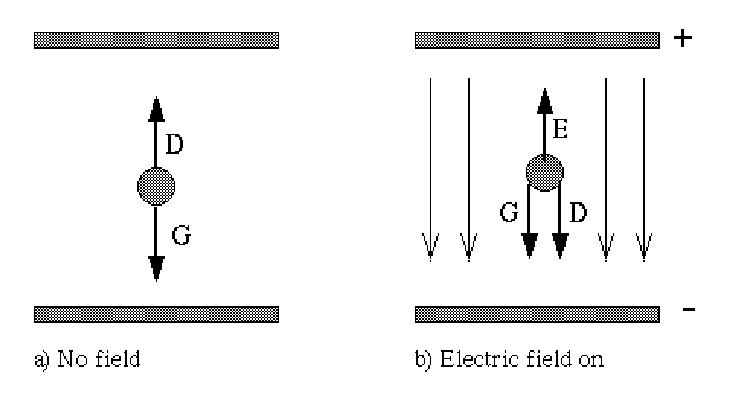
\epsfig{file=Introduction/oil_droplet.eps, height=5cm}
  \caption{
    Forces on an oil-droplet in: \newline
    \hspace*{1.5cm}
           a) Free fall          \newline
    \hspace*{1.5cm}
	   b) Electric field     \newline
    (G=Gravitation, D=Drag, E=Electric force)
  }
  \label{oil_droplet}
\end{center}
\end{figure}

His results were systematically low by about 4\% due to inaccurate
knowledge of the coefficient of viscosity. \newline
The electron charge is -e,
where $e = 1.602 \cdot 10^{-19}C$. All free particles are observed to
have values of electric charge equal to an integer times the
fundamental charge e:

\begin{equation*}
  q=n e
\end{equation*}

where the integer $n=\dots,-1,0,1,\dots$ is the electric charge
\emph{quantum number}.

\subsection*{The Nucleus}

In 1912, Ernest Rutherford and his associates discovered that the
positive charge of the atom is concentrated in a \emph{nucleus}. The
charge of the $\alpha$ particle, discovered by Becquerel, was
determined to be $2e$, and the mass of the $\alpha$ particle was
determined to be about four times the mass of the hydrogen
atom. \newline
A new particle with zero electric charge was discovered by bombarding
beryllium atoms with $\alpha$ particles. James Chadwick showed that
the new particle, the \emph{neutron}, had mass nearly equal to that of
the \emph{proton}.

\subsection*{The Bohr Model of the Atom}

In 1913, Niels Bohr made the first qunatitatively successful model of
the atom. Inspired by the work of Rutherford, Bohr made a planetary
model of the atom; with electrons moving in circular orbits about the
nucleus. This model may seem quite simple in retrospect, but for the
time it was a great advancement of science. In addition to the
classical circular orbits, the second part of Bohr's atomic model
contains a bold hypothesis of new physics. The new physics recognizes
that \emph{angular momentum} is \emph{quantized}; it can take only
certain values:

\begin{equation*}
  L = mvr = n \hbar
\end{equation*}

where $n$ is a positive integer. Solving the energy equations result
in orbits of radius:

\begin{equation*}
  r_n = \frac{n^2\hbar^2}{mke^2}
\end{equation*}

where the \emph{Bohr radius}

\begin{equation*}
  a_0 \equiv r_1 = \frac{\hbar^2}{mke^2} \approx 0.053 nm
\end{equation*}

is in the correct order of magnitude for the size of the atom!

{\bf Planc }





%               The Two First Excited states of Helium
\subsection{The Two First Excited states of Helium}

We will not make any calculations regarding exited states in this
thesis, but it is a really important issue in quantum mechanics. The
ground state energy does not tell much about the 
chemical properties of the atom on its own. Therefore good
approximations of the exited states are needed. Also, when discussing
different numerical approaches for solving the many body-problem,
including linear combinations of exited states may greatly improve
some original approximation to the ground state. Furthermore,
understanding how we include exited states is important for fully
understanding the application of the Slater determinant.
\newline
%
\newline
The state of helium with the $1s$ and the $2s$ orbitals occupied
with one electron each. 








The construction of the
periodic table in the second half of the $19^{\mathrm{th}}$ century
was based on the chemical properties of the different atoms. These
properties were not understood until the development of quantum
mechanics. The electrons are filled from the energetically lowest
orbitals. In the $s$ orbitals only two electrons of different
spins are allowed. Disregarding electron repulsion this would imply
that twice the energy is needed in removing an electron from ground
state helium than from the ground state hydrogen. This due to the 
double electric charge of the helium nucleus. The ionization energy of
hydrogen is $13.60 eV$ and the ionization energy of helium is $24.58
eV$ (ref. \cite{atkins2003}). The electron repulsion thus reduce the
ionization energy by almost $10\%$.
\newline
%
\newline
The early development of quantum theory may be summarized through the
four postulates of quantum mechanics.


%*************** The Postulates of Quantum Mechanics **************
%*
%*
\section{The Postulates of Quantum Mechanics}

A common formulation of quantum mechanics is by means of linear
algebra. In this formulation every state is represented as a (usually
infinite dimensional) complex vector, and an operator is represented
as a complex, linear and hermitian matrix. 
The postulates of quantum mechanics fall naturally into two sets: the
first three, which tell us how the system is depicted at a given time,
and the fourth, which specifies how this picture changes with time. 
\newline

%*                     The First Postulate                              *
%\subsection{The First Postulate}

{\bf \large Postulate 1}
\emph{
The state of a quantum mechanical particle is described by a vector
$\Psi$ in a Hilbert space ${\cal H}$. All the possible states of the
particle are ${\cal H}$ except the zero vector.
\newline
}

The first postulate states that a particle is described as a vector in
the Hilbert space. So a particle with finite degrees of
freedom $\mathbf{x}$ and $\mathbf{p}$ in classical
mechanics, now has infinite degrees of freedom. 
\newline

%*                     The Second Postulate                              *
%\subsection{The Second Postulate}

{\bf \large Postulate 2}
\emph{
Every observable are represented by an Hermitian linear operator in
${\cal H}$. For every classical dynamical variable
$\omega(\mathbf{x},\mathbf{p})$ there is a corresponding quantum
mechanical operator $\Omega$  obtained by operator substitution of the
fundamental position and momentum operators $\mathbf{X}$ and
$\mathbf{P}$, respectively: 
}
%
\begin{equation*}
  \Omega(\mathbf{X},\mathbf{P}) = \omega(\mathbf{x} \to
  \mathbf{X},\mathbf{p} \to \mathbf{P})
\end{equation*}
%
\emph{
The components of $\mathbf{X}$ and $\mathbf{P}$ are operators defined
through the fundamental commutation relation
}

\begin{equation*}
  \left[ X_i, P_j \right] = i \hbar \delta_{ij}
\end{equation*}

The second postulate tell us how to to move from the classical to the
quantum mechanical picture. The observables (or measurable quantities)
are defined through an operator. This operator may be obtained by
simple substitution of the position and the momentum of the
corresponding classical observable.
\newline

%*                     The Third Postulate                              *
%\subsection{The Third Postulate}

{\bf \large Postulate 3}
\emph{
The only possible values obtainable in an (ideal) measurement of an
observable $\Omega$ are its eigenvalues $\omega_n$. Each have a
probability
}
%
\begin{equation*}
  P(\omega_n) = \frac{\int \Psi^* \Phi_n }{\int \Psi^* \Psi }
\end{equation*}
%
\emph{
with $\Phi_n$ the eigenfunction corresponding to the eigenvalue
$\omega_n$. Immediately after a measurement the state collapses into
$\Phi_n$.
}
\newline

The third postulate tells what may be extracted from the quantum
mechanical picture by means of measurements. Note that the eigenvalues
may either have a continuous spectrum or be \emph{quantized}.
\newline


%*                     The Fourth Postulate                              *
%\subsection{The Fourth Postulate}

{\bf \large Postulate 4}
\emph{
The time development of the quantum state $\Psi$ is given by the time
dependent Schr\"odinger equation,
}

\begin{equation*}
  \hat{H} \Psi(\mathbf{x},t) = i\hbar \frac{\delta}{\delta
  t}\Psi(\mathbf{x},t) 
\end{equation*}

The fourth and final postulate defines the Schr\"odinger
equation. This equation describes how the quantum mechanical state
evolve in time.
\newline





\clearpage

\chapter{The Basis of Quantum Mechanics}

%**************** From Classical of Quantum Mechanics *************
%
\section{Introduction to Quantum Mechanics}

In this section we will give a brief introduction to some of the basic
properties of quantum mechanics. For a more thourough introduction to
quantum mechanics there are several references, among other
\cite{rohlf1994}, \cite{shankar1994} and \cite{hemmer1980}.

%*                    Wave-Particle Duality                    *
\subsection{Wave-Particle Duality}

Let us start out with a simple experiment. We send light through a
tiny\footnote{With 'tiny' we mean the approximate size of
the light's wave-length.} slit, and observe the
intensity-pattern on a screen behind the slit. The pattern is
illustrated in figure \ref{singleSlit}.

\begin{figure}[hbtp]
\begin{center}
  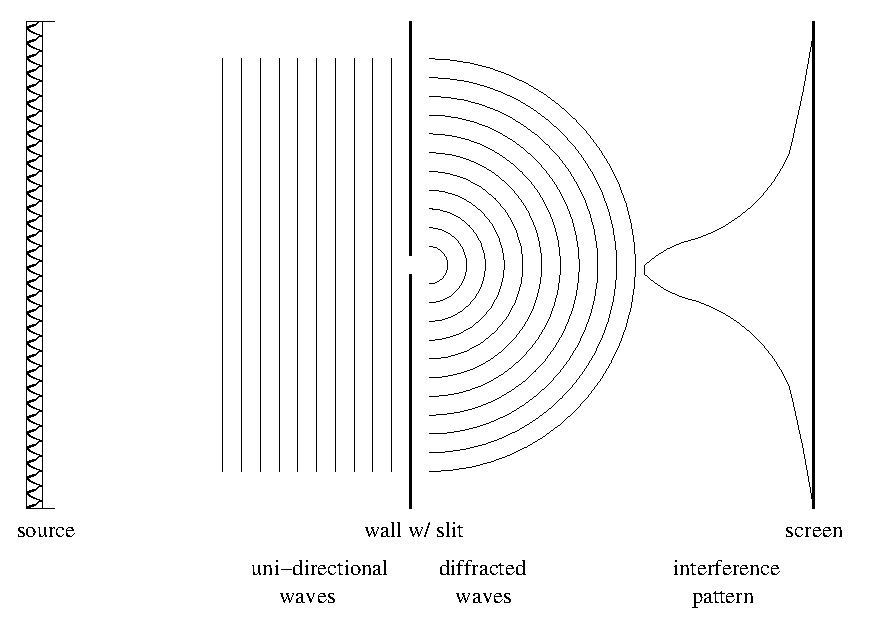
\epsfig{file=Basic_QM/singleSlit.eps, height=6cm}
  \caption{
    Single-slit diffraction
  }
  \label{singleSlit}
\end{center}
\end{figure}

We now expand the above experiment to include two slits, and get an
interference pattern as that given by figure \ref{doubleSlit}. 

\begin{figure}[hbtp]
\begin{center}
  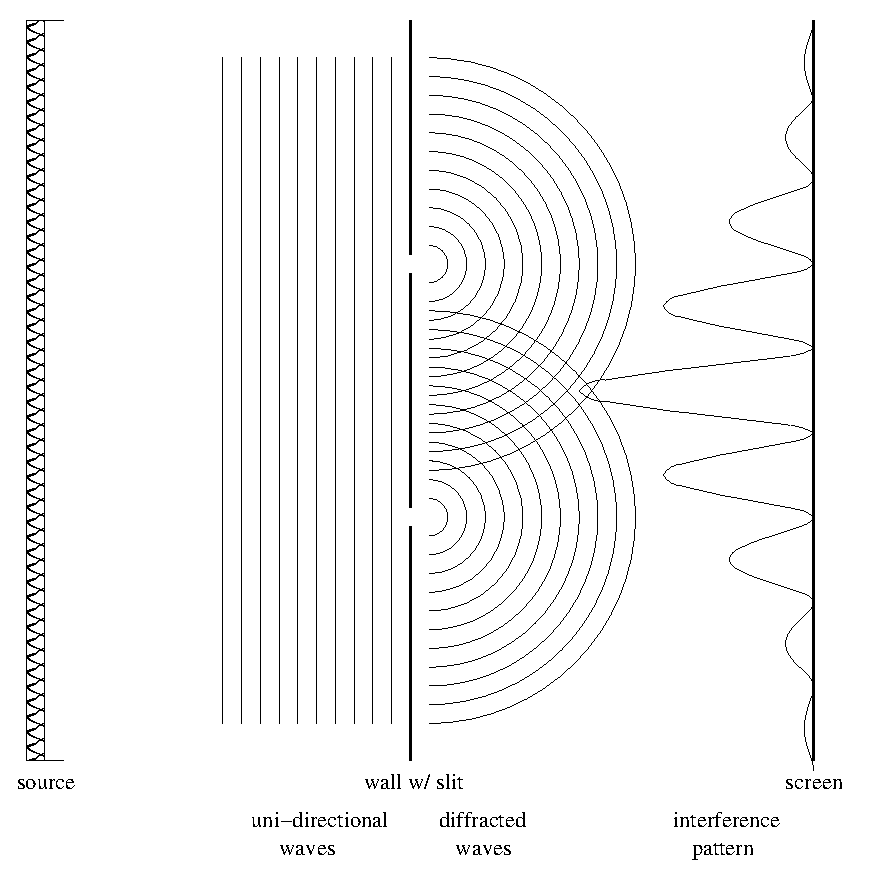
\epsfig{file=Basic_QM/doubleSlit.eps, height=9cm}
  \caption{
    Double-slit diffraction
  }
  \label{doubleSlit}
\end{center}
\end{figure}

If we sent classical particles through a double slit we would expect a
superposition of two single-slit intensity patterns. But this is not
what we actually observe for light.

In addition to the observed diffraction of light,
light may also be reflected and refracted. The reflection of light creates
the mirror image of a mountain on a still lake, and the light of
the sun refracted by a prism creates the rainbow hues. All the above
indicates that light has a wave-behavior. 
\newline
%
\newline

Lets us continue with yet another experiment. We direct light at a
conductive surface as illustrated in figure
\ref{photoElectricEffect}. 

\begin{figure}[hbtp]
\begin{center}
  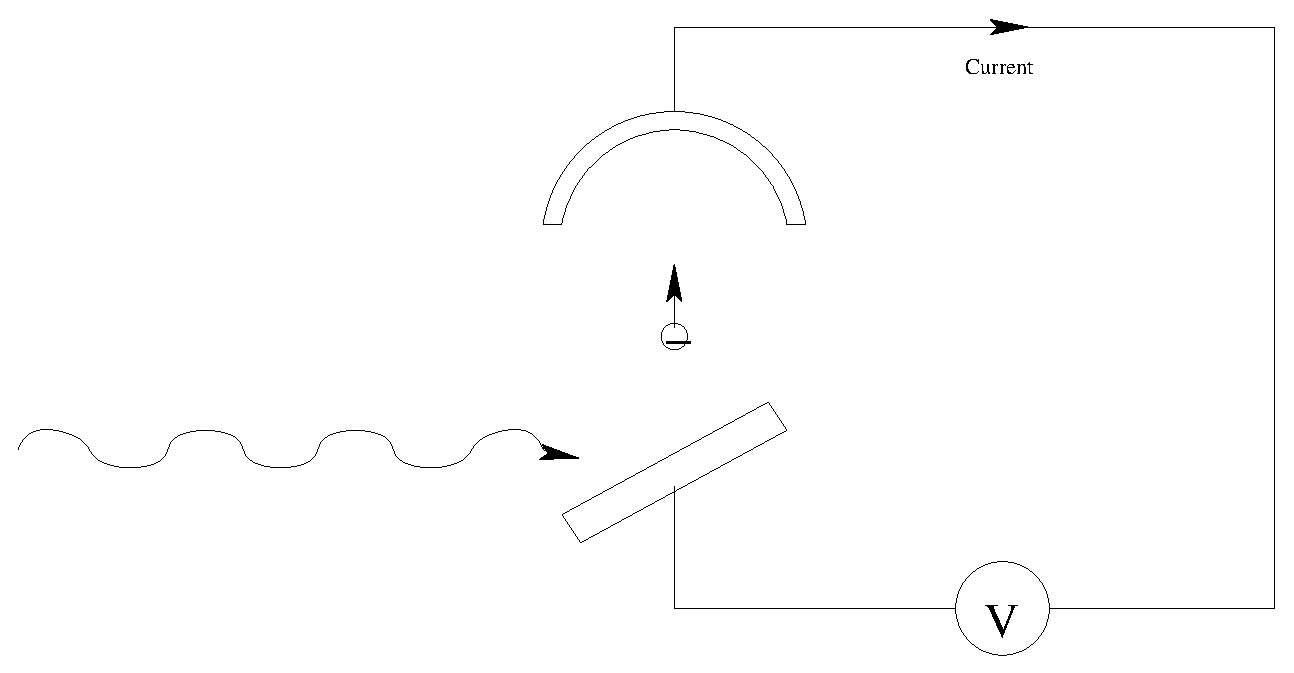
\epsfig{file=Basic_QM/photoElectricEffect.eps, height=6cm}
  \caption{
    Photo-electric effect
  }
  \label{photoElectricEffect}
\end{center}
\end{figure}


The light induces both a voltage and a current in the electric
circuit. What now if we increase the intensity of light? If light
were waves we would expect the voltage to increase, but only the
current is increased. This would indicate that light transfers only a
limited (even quantized!) amount of kinetic energy to the
electrons. But how can this be if light are waves? Who knows, but it's
in the nature of light. Furthermore, there is a lower limit of the
frequency needed to induce the photo-electric effect, dependent on the
photo-cathodic surface the light is directed at. Finally, if light
were waves, we would expect some time delay between when the light
source is turned on and the photo-electric effect is induced, but no
such delay is observed.

We have shown that light has both wave and particle
behavior, and this \emph{wave-particle duality} has no explanation in
classical physics. This duality is present in all objects, but is
measurable only for (sufficiently) small 'particles'.
\newline
%
\newline
%*                          DeBroglie Waves                       *
%\subsection{DeBroglie Waves}

In 1905 Einstein proposed that light has particle properties, 
and that each \emph{quanta} of light ({\bf photon}) has energy
  proportional to its frequency, $\nu$, 

\begin{equation*}
  E = h \nu
\end{equation*}

Here Planck's constant $h=6.626 \cdot 10^{-34} J \cdot s$, is a
fundamental constant of nature. Also in 1905, Einstein demonstrated, in
his special theory of relativity, that the photon has momentum like a
particle  

\begin{equation*}
  p = \frac{h} {\lambda}
\end{equation*}

This idea was generalized by Louis De Broglie, when he in 1924 proposed
that all matter have wave-like properties, and that they thus have a
wavelength ({\bf De Broglie wavelength}), 

\begin{equation*}
  \lambda = \frac{h} {p}
\end{equation*}



%*             Heisenberg's Uncertainty Principle             *
\subsection{Heisenberg's Uncertainty Principle}

In 1925 Heisenberg formulated his {\bf Uncertainty
  Principle}. Heisenberg's uncertainty principle states that one cannot
  measure a particle's position and momentum simultaneously with
  infinite precision.

\begin{equation*}
  \Delta x \Delta p \ge \frac{\hbar}{2}
\end{equation*}

Here $\Delta x$ and $\Delta p$ are the uncertainties in the position
and the momentum, respectively, and the \emph{reduced Plank's constant}
$\hbar = h/2\pi$. Also,

\begin{equation*}
  \Delta E \Delta t \ge \frac{\hbar}{2}
\end{equation*}

where $\Delta E$ and $\Delta t$ are the uncertainties energy and time,
respectively.

A consequence of the uncertainty principle is that
measuring the state of a microscopic system changes the system. 
\newline
%
\newline

Consider the double-slit experiment, depicted in figure
\ref{doubleSlit}, and reduce the intensity to allow only one
particle's to pass the slit at a time. What now? The interference
pattern in the figure now represents the particle's probability
distribution function. But how is this possible? In the classical way
of thinking the particle either passes the upper or the lower
slit. Following this line of thinking would lead to the superposition
of two single-slit experiments. This is not the case! So what then is
the solution? Either the photon is emitted from it's source at one
time, and then moves through both slits at the same time before
hitting the screen, or one simply cannot talk about a path at all.
Who knows?

So what then is the physicists approach?



%*                           The Quantum State                          *
\subsection{The Quantum State}

A proper description of a state allows all the known properties of
a system to be found. For a macroscopic system, the state of a
particle at a given time can be specified by a point in 
{\bf phase space}, i.e. the space spanned by the spatial coordinates
and the momentum coordinates. The energy, spin etc. of a particle, may 
all be found from the state of the particle.

In 1926 Erwin Schr\"odinger developed the idea of the \emph{complex}
{\bf wave function}, $\Psi = \Psi (\mathbf{x},t)$,
which is the state of microscopic systems. Unlike a trajectory the
wave-function has no independent reality. It only bears meaning in
conjunction with its complex conjugate $\Psi^*$ and an {\bf
  operator}. For example $\Psi^* \Psi = |\Psi|^2$ 
may be interpreted as a {\bf probability density} (here the operator
is the identity). For a given time
$t$ this has physical meaning when associated with a region in
space. Furthermore, this interpretation implies that the norm

\begin{equation*}
  \int\limits_{\Omega} |\Psi|^2 d\Omega = 1
\end{equation*}

where $\Omega$ is space. Thus, the wave-function must be
normalizable. 



%*                  Operators and Observables                          *
\subsection{Operators and Observables}

Every {\bf observable} (or measurable quantity) has an operator. The
information available in a wave-function is extracted by using the
operator to calculate an {\bf expectation value}. The expectation
value of an operator, $\left< \hat{{\cal O}} \right>$, is defined as

\begin{equation*}
  \left< \hat{{\cal O}} \right> 
  = \frac {\int \Psi^* \hat{{\cal O}} \Psi}  {\Psi^* \Psi}
\end{equation*}

For each classical variable
$\omega(\mathbf{x},\mathbf{p})$ there corresponds an operator $\Omega$
obtained by operator substitution of the two fundamental operators,

\begin{equation}
  \Omega(\mathbf{\hat{X}},\mathbf{\hat{P}}) = \omega(\mathbf{x} \to
  \mathbf{\hat{X}},\mathbf{p} \to \mathbf{\hat{P}})
  \label{operatorSubstitution}
\end{equation}

The fundamental operators of position and momentum are given by

\begin{equation*}
  \mathbf{\hat{X}} = \mathbf{x}
\end{equation*}

and

\begin{equation*}
  \mathbf{\hat{P}} = -i\hbar \nabla
\end{equation*}

respectively. 



%*            Commutators and Commuting Observables                   *
\subsection{Commutators and Commuting Observables}

An important feature in quantum mechanics is the 
{\bf commutator}. Given two operators $\hat{A}$ and $\hat{B}$ the
commutator is defined by

\begin{equation*}
  \left[ \hat{A}, \hat{B} \right] = \hat{A} \hat{B} - \hat{B} \hat{A}
\end{equation*}

A pair of operators are said to {\bf commute} if their commutator
equals zero. The values of the observables $A$ and $B$ can be known
both precisely and simultaneously, if and only if $\hat{A}$ and
$\hat{B}$ commute. The two fundamental position and momentum operators
does not commute:

\begin{equation*}
  \begin{split} 
  \left[ \hat{X_i}, \hat{P_i} \right] \Psi(\mathbf{x}, t) 
  &= \left[ x_i, -i \hbar \frac{\delta}{\delta x_i} \right] \Psi(\mathbf{x},t)
  = -i \hbar \left( x_i \frac{\delta}{\delta x_i} -
  \frac{\delta}{\delta x_i} x_i \right) \Psi(\mathbf{x},t) \\
  &= -i \hbar \left( x_i \frac{\delta}{\delta x_i} - \left[ x_i
  \frac{\delta}{\delta x_i} + 1 \right] \right) \Psi(\mathbf{x},t) 
  = i \hbar \Psi(\mathbf{x},t)
  \end{split}
\end{equation*}

i.e. $\left[ \hat{X_i}, \hat{P_i} \right] = i \hbar$. These two
observables may therefor not be known simultaneously, which is in
accordance with Heisenberg's uncertainty principle.


%*               Eigenfunctions and Eigenvalues                       *
\subsection{Eigenfunctions and Eigenvalues}

In the late nineteenth century, Anders \AA ngstom made wavelength
measurements of four visible lines emitted by hydrogen. This indicates
that the energy, and thereof the states, of the hydrogen atom are
quantized.  Quantum mechanical states can be described with 
{\bf eigenfunctions} of an operator. If a wave is in an
eigenstate, the observable has a corresponding 
{\bf eigenvalue}. The light waves of the hydrogen spectrum are
actually the photons emitted when the hydrogen atom goes from one
state to another. For an observable ${\cal O}$ with quantum operator
$\hat{{\cal O}}$ this yield the eigenvalue-problem,

\begin{equation*}
  \hat{{\cal O}} \Psi_n = {\cal O}_n \Psi_n
\end{equation*}

where $\Psi_n$ is an eigenstate and ${\cal O}_n$ is an eigenvalue.


%*                      The Hamiltonian                               *
\subsection{The Hamiltonian}

Classically, the total energy of a system is written in a systems 
{\bf Hamiltonian}, $H$. Usually, the Hamiltonian is defined as

\begin{equation*}
  H = T + V
\end{equation*}

where $T$ is the kinetic energy, and $V$ is the potential energy. The
kinetic energy operator of a one-particle system is

\begin{equation*}
  T = \frac{1}{2}m\mathbf{v}^2 = \frac{\mathbf{p}^2}{2m}
\end{equation*}

where $\mathbf{v}$ is the velocity and $\mathbf{p}$ is the
momentum. Performing operator substitution of the two fundamental
operators yield the quantum mechanical operator for the energy

\begin{equation*}
  \hat{H}(\mathbf{\hat{P}}, \mathbf{\hat{X}}, t) =
  \frac{\mathbf{\hat{P}}^2}{2m} + V(\mathbf{\hat{X}}, t)
\end{equation*}

Recalling that the fundamental operators of position and momentum are
given by 

\begin{equation*}
  \mathbf{\hat{X}} = \mathbf{x}
\end{equation*}

and

\begin{equation*}
  \mathbf{\hat{P}} = -i\hbar \nabla
\end{equation*}

the Hamiltonian of a one-particle quantum mechanical system reads

\begin{equation*}
  \hat{H}(\mathbf{x}, t) = -\frac{\hbar^2}{2m} \nabla^2 +
  V(\mathbf{x}, t)
\end{equation*}


%*                 The Schr\"odinger Equation                         *
\subsection{The Schr\"odinger Equation}

The Hamiltonian is the operator of the energy. And the
eigenvalue-problem posed by the Hamiltonian

\begin{equation*}
  \hat{H}(\mathbf{x}, t) \Psi_n(\mathbf{x}, t)  
  = E_n \Psi_n(\mathbf{x}, t) 
\end{equation*}

is called the stationary (or time-independent) Schr\"odinger
equation. The time-dependent Schr\"odinger equation

\begin{equation*}
  \hat{H}(\mathbf{x}, t) \Psi_n(\mathbf{x}, t)  
  = i\hbar \frac{\delta}{\delta t} \Psi_n(\mathbf{x}, t) 
\end{equation*}

will not be studied in this thesis. However, as a fundamental equation
of quantum mechanics it sort of found its way into this thesis anyhow.

%*                     The Hilbert Space                              *
\subsection{The Hilbert Space}

A common formulation of quantum mechanics is by means of linear
algebra. In this formulation every state is represented as a (usually
infinite dimensional) complex vector, and an operator is represented
as a complex, linear and hermitian matrix. 
The {\bf Hilbert space} is the (usually infinite dimensional) complex
linear state space. The Hilbert space is dual in that every vector
$\Psi$ is associated with the dual vector $\Psi^*$.



%*************** The Postulates of Quantum Mechanics **************
%*
%*
\subsection{The Postulates of Quantum Mechanics}

We are now ready to formulate the postulates of quantum mechanics. The
postulates fall naturally into two sets: the first three, which tell
us how the system is depicted at a given time, and the last, which
specifies how this picture changes with time. 
\newline

%*                     The First Postulate                              *
%\subsection{The First Postulate}

{\bf \large Postulate 1}
\emph{
The state of a quantum mechanical particle is described by a vector
$\Psi$ in a Hilbert space ${\cal H}$. All the possible states of the
particle are ${\cal H}$ except the zero vector.
\newline
}

The first postulate states that a particle is described as a vector in
the Hilbert space. So a classical particle with finite\footnote{Six
  degrees of freedom for the three-dimensional case.} degrees of
freedom, $\mathbf{x}$ and $\mathbf{p}$, in classical
mechanics, now has infinite degrees of freedom. 
\newline

%*                     The Second Postulate                              *
%\subsection{The Second Postulate}

The second postulate defines the quantum operator for the observables
(or measurable quantities). !!! Some more intro here !!!
\newline

{\bf \large Postulate 2}
\emph{
Every observable are represented by an Hermitian linear operator in
${\cal H}$. For every classical dynamical variable
$\omega(\mathbf{x},\mathbf{p})$ there corresponds an operator $\Omega$ 
obtained by operator substitution of the fundamental position and
momentum operators $\mathbf{X}$ and $\mathbf{P}$, respectively:
}
%
\begin{equation*}
  \Omega(\mathbf{X},\mathbf{P}) = \omega(\mathbf{x} \to
  \mathbf{X},\mathbf{p} \to \mathbf{P})
\end{equation*}
%
\emph{
The components of $\mathbf{X}$ and $\mathbf{P}$ are operators defined
through the fundamental commutation relation
}

\begin{equation*}
  \left[ X_i, P_j \right] = i \hbar \delta_{ij}
\end{equation*}

%*                     The Third Postulate                              *
%\subsection{The Third Postulate}

{\bf \large Postulate 3}
\emph{
The only possible values obtainable in an (ideal) measurement of an
observable $\Omega$ are its eigenvalues $\omega_n$. Each have a
probability
}
%
\begin{equation*}
  P(\omega_n) = \frac{\int \Psi^* \Phi_n }{\int \Psi^* \Psi }
\end{equation*}
%
\emph{
with $\Phi_n$ the eigenfunction corresponding to the eigenvalue
$\omega_n$. Immediately after a measurement the state collapses into
$\Phi_n$.
}
\newline

Note that the eigenvalues may have a continuous spectrum.
\newline


%*                     The Fourth Postulate                              *
%\subsection{The Fourth Postulate}

The fourth and final postulate defines the Schr\"odinger equation.
\newline

{\bf \large Postulate 4}
\emph{
The time development of the quantum state $\Psi$ is given by the time
dependent Schr\"odinger equation,
}

\begin{equation*}
  \hat{H} \Psi(\mathbf{x},t) = i\hbar \frac{\delta}{\delta
  t}\Psi(\mathbf{x},t) 
\end{equation*}

%*                Bosons and Fermions                                *
\subsection{Bosons and Fermions}

spin half or integer


%*                       The Pauli Principle                         *
\subsection{The Pauli Principle}




\clearpage

\chapter{Atomic Physics}
\label{AtomicPhysics}


In this chapter the basic principles and difficulties of atomic
physics are outlined through investigation of the hydrogen and helium
atoms. Applications of quantum mechanics to the atomic problem result in
a partial integro-differential equation. This equation cannot be
solved analytically except for the special case of the hydrogen
atom. The solutions of the hydrogen atom provide useful insights
regarding the nature of the atoms, but difficulties arise when we add
one or more electrons. This is mainly because the strength of the
electron-electron interactions is comparable to the nucleus-electron
interaction.

\section{Basics}

\subsection{The Atomic Problem}
\label{TheAtomicProblem}

The Hamiltonian for an $N$-electron atomic system consists of two terms

\begin{equation}
  \hat{H}(\mathbf{x}) 
  = \hat{T}(\mathbf{x}) 
  + \hat{V}(\mathbf{x}); 
\label{hamiltonOperatorFull}
\end{equation}

the kinetic and the potential energy operator. Here $\mathbf{x} =
\left\{ \mathbf{x}_1, \mathbf{x}_2, \dots \mathbf{x}_N \right\}$  is
the spatial and spin degrees of freedom associated with the different
particles. The classical kinetic energy  

\begin{equation*}
  T= \frac{\mathbf{P^2}}{2m} + \sum_{j=1}^N \frac{\mathbf{p}_j^2}{2m}
\end{equation*}

is transformed to the quantum mechanical kinetic energy operator by 
operator substitution of the momentum ($p_k \to -i\hbar
\partial/\partial x_k$)

\begin{equation}
  \hat{T}(\mathbf{x}) = -\frac{\hbar^2}{2M}\nabla^2_0
  -\sum_{i=1}^{N}\frac{\hbar^2}{2m}\nabla^2_i.
\label{kineticEnergyOperatorFull}
\end{equation}

Here the first term is the kinetic energy operator of the nucleus,
the second term is the kinetic energy operator of the electrons,
$M$ is the mass of the nucleus and $m$ is the electron mass. The
potential energy operator is given by

\begin{equation}
  \hat{V}(\mathbf{x}) = 
  - \sum_{i=1}^{N} \frac{Ze^2}{(4\pi \epsilon_0)r_i}
  + \sum_{i=1,i<j}^{N} \frac{e^2}{(4\pi \epsilon_0)r_{ij}},
\label{potentialEnergyOperatorFull}
\end{equation}

where the $r_i$'s are the electron-nucleus distances and the
$r_{ij}$'s are the inter-electronic distances. 
\newline
%
\newline
We seek to find controlled and well understood approximations in order
to reduce the complexity of the above equations. The
\emph{Born-Oppenheimer approximation} is a commonly used
approximation, in which the motion of the nucleus is disregarded.


%*                The Born-Oppenheimer Approximation                *
\subsection{The Born-Oppenheimer Approximation}

In a system of interacting electrons and a nucleus there will usually
be little momentum transfer between the two types of particles due to
their differing masses. The forces between the particles are 
of similar magnitude due to their similar charge. If one assumes
that the momenta of the particles are also similar, the nucleus
must have a much smaller velocity than the electrons due to its far
greater mass. On the time-scale of nuclear motion, one can therefore
consider the electrons to relax to a ground-state given by the
Hamiltonian of eqs.~(\ref{hamiltonOperatorFull}),
(\ref{kineticEnergyOperatorFull}) and
(\ref{potentialEnergyOperatorFull}) with the nucleus at a fixed
location. This separation of the electronic and nuclear degrees of
freedom is known as the Born-Oppenheimer approximation. 
\newline
%
\newline
In the center of mass system the
kinetic energy operator reads (ref. \cite{bransden1983})

\begin{equation}
  \hat{T}(\mathbf{x}) = -\frac{\hbar^2}{2(M+Nm)}\nabla^2_{CM}
  -\frac{\hbar^2}{2\mu}\sum_{i=1}^{N}\nabla^2_i
  -\frac{\hbar^2}{M}\sum_{i>j}^{N}\nabla_i\cdot\nabla_j,
  \label{centerOfMassKineticEnergyOperator}
\end{equation}

while the potential energy operator remains unchanged. Note that the
Laplace operators $\nabla^2_i$ now are in the center of mass reference
system.
\newline
%
\newline
The first term of eq.~(\ref{centerOfMassKineticEnergyOperator})
represents the kinetic energy operator of the center of mass. The
second term represents the sum of the kinetic energy operators of the
$N$ electrons, each of them having their mass $m$ replaced by the
reduced mass $\mu = mM/(m+M)$ because of the motion of the
nucleus. The nuclear motion is also responsible for the third term,
or the \emph{mass polarization} term.
\newline
%
\newline
The nucleus consists of protons
and neutrons. The proton-electron mass ratio is about
$1 / 1836$ and the neutron-electron mass ratio is about
$1 / 1839$, so regarding the nucleus as stationary is a natural
approximation. Taking the limit $M\to \infty$ in
eq.~(\ref{centerOfMassKineticEnergyOperator}), the kinetic energy 
operator reduces to

\begin{equation}
  \hat{T} = -\sum_{i=1}^{N}\frac{\hbar^2}{2m}\nabla^2_i
\end{equation}

The Born-Oppenheimer approximation thus disregards both the kinetic
energy of the center of mass as well as the mass polarization term.
The effects of the Born-Oppenheimer approximation are quite small and
they are also well accounted for.
However, this simplified electronic Hamiltonian remains very difficult
to solve, and analytical solutions do not exist for general systems
with more than one electron. The Born-Oppenheimer approximation will
be used for the rest of this thesis.  
\newline
%
\newline
The first term of eq.~(\ref{potentialEnergyOperatorFull}) is the
nucleus-electron potential and the second term is the
electron-electron potential. The inter-electronic potentials are the
main problem in atomic physics. Because of these terms, the
Hamiltonian cannot be separated into one-particle parts, and the
problem must be solved as a whole. A common approximation is to regard
the effects of the electron-electron interactions either as averaged
over the domain or by means of introducing a density functional, such as
by Hartree-Fock (HF) or Density Functional Theory (DFT). These
approaches are actually very efficient, and about $99\%$ or more of
the electronic energies are obtained for most HF calculations.
Other observables are usually obtained to an accuracy of about
$90-95\%$ (ref. \cite{helgaker2002}).  The main effort of the
advanced numerical procedures is to reduce the errors these
approximations induce. These issues will be discussed in detail in
chapter \ref{NumericalApproaches}. But first we simplify the atomic
problem further by using atomic units. 

%*                          Atomic Units                           *
\subsection{Atomic Units}

Numerical methods require proper scaling of the system in
question. In atomic systems we scale to atomic units by setting
$m=e=\hbar=4\pi\epsilon_0=1$, see table \ref{atomicUnits}. 

\begin{table}[hbtp]
\begin{center} {\large \bf Atomic Units} \\ 
$\phantom{a}$ \\
\begin{tabular}{llc}
\hline\\ 
{\bf Quantity}                 & {\bf SI}               & {\bf Atomic unit}\\
Electron mass, $m$               & $9.109\cdot 10^{-31}$ kg & 1 \\
Charge, $e$                      & $1.602\cdot 10^{-19}$ C  & 1 \\
Planck's reduced constant, $\hbar$& $1.055\cdot 10^{-34}$ Js& 1 \\       
Permittivity, $4\pi\epsilon_0$   & $1.113\cdot 10^{-10}$ C$^2$ J$^{-1}$ m$^{-1}$&1\\
Energy, $\frac{e^2}{4\pi\epsilon_0 a_0}$ & $27.211$ eV       & 1 \\
Length, $a_0=\frac{4\pi\epsilon_0 \hbar^2}{me^2}$&$0.529\cdot10^{-10}$ m&1\\ [10pt]      
\hline
\end{tabular} 
\end{center}
\caption{Scaling from SI to atomic units}
\label{atomicUnits}
\end{table}

In this way the atomic problem is simplified to

\begin{equation}
  \left[-\sum_{i=1}^N \frac{1}{2} \nabla^2_i 
    - \sum_{i=1}^N \frac{Z}{r_i} + \sum_{i<j}^N \frac{1}{r_{ij}} 
    \right] \Psi(\mathbf{x}) = E \Psi(\mathbf{x}).
  \label{SchrodingerBornOppenheimerAtomicUnits}
\end{equation}

This is the equation we want to solve in atomic physics. The
introduction of atomic units serves two purposes. In addition to
making the equation easier to work with because of the neglected
units, the atomic units also have an important numerical feature. When
solving numerical problems the different quantities involved must have
proper scaling; they must be in the same order of magnitude. Failing
to do so may result in loss of numerical precision.


%*******************************************************************
%*                      The Hydrogen Atom                          *
%*******************************************************************
\section{The Hydrogen Atom}
\label{TheHydrogenAtom}

The solutions of the hydrogen atom form the basis of our
understanding of the many-electron atom. The Hamiltonian of the
hydrogen atom reads 

\begin{equation}
  \hat{H} = -\frac{1}{2} \nabla^2  + V(r),
  \label{HydrogenHamiltonian}
\end{equation}

where $V(r) = - Z/r$. The nucleus charge $Z$ equals unity for the
hydrogen atom, but since the solutions to hydrogen-like atoms are
important, we keep it throughout our calculations. In polar coordinates
the Laplacian is given by (ref. \cite{rottmann2003})

\begin{equation}
  \nabla^2 = \frac{1}{r^2}\left[
    \frac{\partial}{\partial r} \left( r^2 \frac{\partial}{\partial r}\right)+
    \frac{1}{sin^2 \theta} \frac{\partial^2}{\partial \phi}+
    \frac{1}{sin \theta}\frac{\partial}{\partial \theta} \left( sin \theta
    \frac{\partial}{\partial \theta} \right)
    \right].
\label{laplacianRottmann}
\end{equation}

Introduction of this term, combined with the fact that the potential is
spherically symmetric, allows us to separate the radial part and the
angular part of the equation; $\Psi(r,\theta, \phi) =
R(r) \cdot Y(\theta,\phi)$. The solutions of the angular equation are
known as the spherical harmonics $Y_{lm_l}(\theta, \phi)$. The first
few spherical harmonics are listed in table \ref{sphericalHaromical}.
\newline

\begin{table}[hbtp]
\begin{center} {\large \bf Spherical Harmonics} \\ 
$\phantom{a}$ \\
\begin{tabular}{ccccc}
\hline\\ 
$m_l\backslash l$ & \phantom{AA}0\phantom{AA}
& \phantom{AA}1\phantom{AA} & \phantom{AA}2\phantom{AA} &
\phantom{AA}3\phantom{AA} \\ 
\hline\\ 
+3 &                      &
&
&$-\frac{1}{8}(\frac{35}{\pi})^{1/2}sin^3\theta e^{+ 3i\phi}$
\\ [7pt] 

+2 &                      &
&$\frac{1}{4}(\frac{15}{2\pi})^{1/2}sin^2\theta e^{+ 2i\phi}$
&$\frac{1}{4}(\frac{105}{2\pi})^{1/2}cos\theta sin^2\theta e^{+ 2i\phi}$     \\ [7pt]

+1 &  
&$-\frac{1}{2}(\frac{3}{2\pi})^{1/2}sin\theta
e^{+i\phi}$&$-\frac{1}{2}(\frac{15}{2\pi})^{1/2}cos\theta sin\theta
e^{+ i\phi}$&$-\frac{1}{8}(\frac{21}{2\pi})^{1/2}(5cos^2\theta
-1)sin\theta e^{+ i\phi}$\\ [7pt] 

 0 &$\frac{1}{2\pi^{1/2}}$&$\frac{1}{2}(\frac{3}{\pi})^{1/2}cos\theta$
 &$\frac{1}{4}(\frac{5}{\pi})^{1/2}(3cos^2\theta-1)$
 &$\frac{1}{4}(\frac{7}{\pi})^{1/2}(2-5sin^2\theta)cos\theta$
 \\ [7pt] 

-1 &  
 &$+\frac{1}{2}(\frac{3}{2\pi})^{1/2}sin\theta
 e^{-i\phi}$&$+\frac{1}{2}(\frac{15}{2\pi})^{1/2}cos\theta sin\theta
 e^{- i\phi}$&$+\frac{1}{8}(\frac{21}{2\pi})^{1/2}(5cos^2\theta
 -1)sin\theta e^{- i\phi}$\\ [7pt] 

-2 &                      &
 &$\frac{1}{4}(\frac{15}{2\pi})^{1/2}sin^2\theta e^{- 2i\phi}$
 &$\frac{1}{4}(\frac{105}{2\pi})^{1/2}cos\theta sin^2\theta e^{- 2i\phi}$     \\ [7pt]

-3 &                      &
&
&$+\frac{1}{8}(\frac{35}{\pi})^{1/2}sin^3\theta e^{- 3i\phi}$
\\ [7pt] 
\hline
\end{tabular} 
\end{center}
\caption{Spherical harmonics $Y_{lm_l}$ for the lowest $l$ and $m_l$
  values (taken from ref. \cite{atkins2003}).} 
\label{sphericalHaromical}
\end{table}

The spherical harmonics introduce two quantum numbers 
$l = 0,1,2,\dots$ and $m_l = -l, -(l-1), \dots, (l-1), l$. 
These quantum numbers are called the 
\emph{orbital angular momentum} and the \emph{magnetic quantum
number}, respectively. It is worth noticing that the spherical
harmonics are independent of the shape of a spherical symmetric
potential $V(r)$. The radial and the angular part are interconnected
through the separation constants introduced when separating the
equations. For the radial wave-function 

\begin{equation}
  \left[ -\frac{1}{2} \frac{1}{r^2}\frac{\partial}{\partial r} 
    \left( r^2 \frac{\partial}{\partial r}\right)  
    + V(r) + \frac{l(l+1)}{r^2} \right]
  R(r) = E R(r).
\label{hydrogenRadialEquation}
\end{equation}

we therefore have a term including the angular momentum $l$.
The first few non-normalized radial solutions of equation
(\ref{hydrogenRadialEquation}) are listed in table
\ref{hydrogenRadialFunctions}.
\newline


\begin{table}[hbtp]
\begin{center} {\large \bf Hydrogen-Like Atomic Radial Functions} \\ 
$\phantom{a}$ \\
\begin{tabular}{cccc}
\hline\\ 
$l\backslash n$ & \phantom{AA}1\phantom{AA}
& \phantom{AA}2\phantom{AA} & \phantom{AA}3\phantom{AA}  \\ 
\hline\\ 
0 & $e^{-Zr}$ & $(2-r)e^{-Zr/2}$ & $(27-18r+2r^2)e^{-Zr/3}$ \\[7pt]
1 & & $re^{-Zr/2}$ & $r(6-r)e^{-Zr/3}$\\[7pt]
2 & & & $r^2e^{-Zr/3}$ \\[7pt]
\hline
\end{tabular} 
\end{center}
\caption{The first few radial functions of the hydrogen-like atoms
  (taken from ref. \cite{rohlf1994}).} 
\label{hydrogenRadialFunctions}
\end{table}

The states

\begin{equation}
  \Psi_{nlm_l}(r,\theta, \phi) =R_{nl}(r) \cdot Y_{lm_l}(\theta,\phi),
\label{totalHydrogenWavefunction}
\end{equation}

now have three quantum numbers $n$, $l$, $m_l$, where the
\emph{principal quantum number} can take any positive integer
$n=1,2,\dots$. By the introduction of 
quantum numbers the electron may only occupy distinct states or
\emph{eigenstates}, and the corresponding \emph{eigenenergy} is thus
quantized. The eigenenergies

\begin{equation*}
  E_{n} = -\frac{1}{2n^2},
\end{equation*}

are independent of the orbital angular momentum and the magnetic
quantum number. The eigenstates are therefore \emph{degenerate};
several distinct states share the same energy $E_n$. For a given $n$
we have a degeneracy both with respect to varying values of $l$ and of
$m_l$. Furthermore, we have yet another degeneracy associated with the
two possible values of the electronic spin $m_s$ ($=\pm 1/2$).
\newline
%
\newline
The degeneracy due to the magnetic and spin quantum numbers becomes
clear when applying a magnetic field. The magnetic field removes the
degeneracy by splitting the energy levels. 
The degeneracy of different orbital angular momenta of the hydrogen
atom is removed in multi-electronic systems. 
Higher angular momentum lead to higher energy. 
This result 
is manifested by the way the atoms are classified in the periodic
table. States with different orbital angular momenta are for
historical reasons assigned the letters $s$, $p$, $d$, $f$, etc. where
$s$ corresponds to $l=0$, $p$ to $l=1$ and so forth. For example
$2p$ is assigned to a state with $n=2$ and $l=1$. The orbitals are
energetically arranged in the order $1s$, $2s$, $2p$, $3s$, $3p$,
$4s$, $3d$, $4p$, $5s$, $4d$, $5p$, $6s$, $4f$, $5d$, $6p$, etc.,
which explains the general trends of the periodic table.
\newline
%
\newline
A problem with the spherical harmonics of table
\ref{sphericalHaromical} is that they are complex. The introduction of
\emph{solid harmonics}, see ref. \cite{helgaker2002}, allows the use
of real orbital wave-functions for a wide range of applications. The
complex solid harmonics ${\cal Y}_{lm_l}(\mathbf{r})$ are related to
the spherical harmonics  $Y_{lm_L}(\mathbf{r})$ through

\begin{equation*}
  {\cal Y}_{lm_l}(\mathbf{r}) = r^l Y_{lm_l}(\mathbf{r}).
\end{equation*}

By factoring out the leading $r$-dependency of the radial-function
(see for example \cite{shankar1994} \newline \newline)

\begin{equation*}
  {\cal R}_{nl}(\mathbf{r}) = r^{-l} R_{nl}(\mathbf{r}),
\end{equation*}

we obtain a relationship similar to that of
eq.~(\ref{totalHydrogenWavefunction}), namely

\begin{equation*}
  \Psi_{nlm_l}(r,\theta, \phi) %=R_{nl}(r) \cdot Y_{lm_l}(\theta,\phi)
  = {\cal R}_{nl}(\mathbf{r})\cdot{\cal Y}_{lm_l}(\mathbf{r}).
%\label{totalSolidHydrogenWavefunction}
\end{equation*}

For the theoretical development of the \emph{real solid harmonics} see
ref. \cite{helgaker2002}. Here Helgaker \emph{et al} first 
express the complex solid harmonics, $C_{lm_l}$, by (complex) Cartesian
coordinates, and arrive at the real solid harmonics, $S_{lm_l}$, through
the unitary transformation

\begin{equation*}
  \left( \begin{split} &\phantom{i} S_{lm_l} \\ 
    &S_{l,-m_l} \end{split} \right) 
  = \frac{1}{\sqrt{2}} \left(        \begin{split}
    (-1)^m_l \phantom{a} & \phantom{aa} 1 \\ 
    -(-1)^m_l i & \phantom{aa} i       \end{split} \right)  
  \left( \begin{split} &\phantom{i} C_{lm_l} \\ 
    &C_{l,-m_l} \end{split} \right).
\end{equation*}

This transformation will not alter any physical quantities that are
degenerate in the subspace consisting of opposite magnetic quantum
numbers (the angular momentum $l$ is equal for both these cases). This
means for example that the above transformation does not alter the
energies, unless an external magnetic field is applied to the
system. Henceforth, we will use the solid harmonics, and note that
changing the spherical potential beyond the Coulomb potential will not
alter the solid harmonics. The lowest-order real solid harmonics are
listed in table \ref{solidHarmonics}.

\begin{table}[hbtp]
\begin{center} {\large \bf Real Solid Harmonics} \\ 
$\phantom{a}$ \\
\begin{tabular}{ccccc}
\hline\\ 
$m_l\backslash l$ & \phantom{AA}0\phantom{AA}
& \phantom{AA}1\phantom{AA} & \phantom{AA}2\phantom{AA} &
\phantom{AA}3\phantom{AA} \\ 
\hline\\ 
+3& & &
&$\frac{1}{2}\sqrt{\frac{5}{2}}(x^2-3y^2)x$ \\ [7pt] 
+2& & &$\frac{1}{2}\sqrt{3}(x^2-y^2)$&$\frac{1}{2}\sqrt{15}(x^2-y^2)z$
\\ [7pt] 
+1& &x&$\sqrt{3}xz$
&$\frac{1}{2}\sqrt{\frac{3}{2}}(5z^2-r^2)x$ \\ [7pt] 
0&1&y&$\frac{1}{2}(3z^2-r^2)$       &$\frac{1}{2}(5z^2-3r^2)x$ \\
 [7pt] 
-1& &z&$\sqrt{3}yz$
&$\frac{1}{2}\sqrt{\frac{3}{2}}(5z^2-r^2)y$ \\ [7pt] 
-2& & &$\sqrt{3}xy$                  &$\sqrt{15}xyz$ \\ [7pt] 
-3& & &
&$\frac{1}{2}\sqrt{\frac{5}{2}}(3x^2-y^2)y$ \\ [7pt] 
\hline
\end{tabular} 
\end{center}
\caption{The first-order real solid harmonics ${\cal Y}_{lm_l}$ (taken from
  ref. \cite{atkins2003}).} 
\label{solidHarmonics}
\end{table}






%*****************************************************************
%*                      The Helium Atom                          *
%*****************************************************************
\section{The Helium Atom}
\label{TheHeliumAtom}

The helium atom cannot be solved analytically. The numerical
solutions, however, are in excellent agreement with
experiments, see for example ref. \cite{coldwell1997}. We will not
go into the details of such accurate approaches, but rather illustrate
how to generate an approximate wave-function through application of 
perturbative and variational methods.
\newline
%
\newline
The Hamiltonian of the helium atom is

\begin{equation}
  \hat{H} = -\frac{1}{2} \nabla_1^2 - \frac{1}{2} \nabla_2^2  -
  \frac{2}{r_1} - \frac{2}{r_2} + \frac{1}{r_{12}}.
  \label{HeliumHamiltonian}
\end{equation}


%*                   The Perturbative Approach                   *
\subsection{The Perturbative Approach}
In the perturbative approach controlled approximations are made so
that the initial problem is transformed to an \emph{unperturbed} problem
where the solutions are easy to obtain. The controlled approximations
are treated as \emph{perturbations} of the unperturbed problem and
added into the system by including higher and higher corrections of
the perturbation. A requirement of the perturbative approach is that
the perturbations are small compared to the unperturbed values.
Straightforward perturbation of the helium atom is acquired if we
first disregard the electron-electron repulsion, and then add it as a
perturbative correction. 
\newline
%
\newline
Without the inter-electronic 
repulsion we get a separable Hamiltonian

\begin{equation*}
  \hat{H} = -\frac{1}{2} \nabla_1^2 - \frac{1}{2} \nabla_2^2  -
  \frac{2}{r_1} - \frac{2}{r_2} = \hat{h}_1 + \hat{h}_2,
\end{equation*}

and we may solve the two one-particle equations independently. The
unperturbed wave-function becomes the product of two hydrogen atom
solutions (given by equation (\ref{totalHydrogenWavefunction}))


\begin{equation*}
  \Psi_{n_1 l_1 m_{l,1} n_2 l_2 m_{l,2}}^{(0)}
  (r_1, \theta_1, \phi_1, r_2, \theta_2, \phi_2)=
  \Psi_{n_1 l_1 m_{l,1}}(r_1, \theta_1, \phi_1)
  \Psi_{n_2 l_2 m_{l,2}}(r_2, \theta_2, \phi_2)
\end{equation*}

with the nucleus charge $Z=1$ replaced by $Z=2$. This gives the
energy

\begin{equation}
  E_{n_1n_2}^{(0)} = -2\left(\frac{1}{n_1^2}+\frac{1}{n_2^2}\right),
\label{unperturbedHeliumEnergy}
\end{equation}

where the superscript ${(0)}$ indicates the unperturbed energy. For
the ground state we define the product   

\begin{equation*}
  \Psi_{1,0,0}(r_1, \theta_1, \phi_1) 
  \Psi_{1,0,0}(r_2, \theta_2, \phi_2) 
  \equiv \Psi_{1s}(1) \Psi_{1s}(2),
\end{equation*}

The first order correction to the energy is then

\begin{equation}
  J \equiv E_{n_1n_2}^{(1)} - E_{n_1n_2}^{(0)} 
%  = \int \Psi_{1s}(1)^* \Psi_{1s}(2)^* \frac{1}{r_{12}}
%  \Psi_{1s}(1) \Psi_{1s}(2) d\tau_1 d\tau_2 
  = \int |\Psi_{1s}(1)|^2 \frac{1}{r_{12}}
  |\Psi_{1s}(2)|^2 d\tau_1 d\tau_2 ,
\label{CoulombIntegral}
\end{equation}

which is called the \emph{Coulomb integral} and often denoted by
$J$. The Coulomb integral is commonly encountered in the approximative 
methods of many-body quantum mechanics, and has an easy
interpretation. The term $|\Psi_{1s}(1)|^2 d\tau_1$ is the probability
of finding electron $1$ in the volume element $d\tau_1$, and when
multiplied with the charge $-1$ (in atomic units) it represents the
\emph{charge density} of that region. Similarly $-|\Psi_{1s}(2)|^2
d\tau_2$ is the charge density of electron $2$ in the volume element
$d\tau_2$. The Coulomb integral of eq.~(\ref{CoulombIntegral}) may
therefore be interpreted as the averaged contribution of the Coulomb
repulsion between the two electrons. The value of the Coulomb integral
is $J = 1.25$ according to ref. \cite{atkins2003}. This gives a first
order approximation to the ground state energy

\begin{equation*}
  E_0^{(1)} = - 2 - 2 + 1.25 = - 2.75.
\end{equation*}

This result is not in perfect agreement with the experimental value
$E_0=-2.9037$. However, it is a clear indication that we are on the
right track. One of the reasons for the disagreement is that the
perturbation is not at all small, so first-order perturbation theory
cannot be expected to lead to a reliable result.


%*                   The Variational Approach                   *
\subsection{The Variational Approach}

A different way of solving the helium atom is the use of a
\emph{variational} approach. Here we start out by guessing a
parametrized form of a \emph{trial wave-function}
$\Psi_{\mathbf{\alpha}}$, where  
$\mathbf{\alpha} = (\alpha_1, \alpha_2,\dots,\alpha_M)$  
denotes the set of variation parameters. Then we optimize these
parameters in accordance with the 
\emph{variational principle}; the energy expectation value of a
variational wave-function provides an upper bound to the true ground
state energy

\begin{equation*} 
  \frac{\int \Psi_{\mathbf{\alpha}}^* \hat{H}
  \Psi_{\mathbf{\alpha}} d\tau}{\int \vert
  \Psi_{\mathbf{\alpha}}\vert^2 d\tau} \ge E_0.
\end{equation*}

The variational principle of quantum mechanics may be derived by
expanding a normalized trial wave-function, $\Psi_{\mathbf{\alpha}}$,
in terms of the exact orthonormal eigenstates $\left\{ \psi_i
\right\}$ of the Hamiltonian

\begin{equation*} 
  \psi_{\mathbf{\alpha}}=\sum_{i=0}^{\infty} c_{i} \psi_i,
\end{equation*}

where the expansion coefficients $c_{i}$ are normalized

\begin{equation*} 
  \sum_{i=0}^{\infty} \vert c_{i}\vert^2=1. 
\end{equation*}

The expectation of the many-body Hamiltonian $\hat{H}$ is
then evaluated as

\begin{equation*} 
  \langle E_{\mathbf{\alpha}} \rangle =  
 \sum_{i=0}^{\infty} \vert c_{i}\vert^{2} \epsilon_{i},
\end{equation*}

where $\epsilon_{i}$ and $\psi_i $ fulfills the stationary
Schr\"odinger equation

\begin{equation*} 
  \hat{H} \psi_i = \epsilon_{i} \psi_i.
\end{equation*}

The expectation value of the trial energy
must therefore be greater than or equal to the true ground state
energy

\begin{equation*} 
  \langle E_{\mathbf{\alpha}} \rangle \ge \langle E_0 \rangle = \epsilon_0,
\end{equation*}

as $\epsilon_{i} \ge \epsilon_{0}$. The variational energy
computed using $\psi_{\mathbf{\alpha}}$ thus provides an upper bound
for the true ground state energy. Therefore, our strategy is to 
search for the variational parameters that give us the lowest
variational energy. 
\newline
%
\newline
The difficulties in the variational method are to find a good
variational wave-function, to evaluate the energy expectation value and
to find the energy minimum in parameter space. There are several ways
to generate the trial wave-function, and we will return to some of
these in chapter \ref{NumericalApproaches}. One simple approach is to
start with a product of two variational hydrogen $1s$ solutions 

\begin{equation*} 
  \psi_{\alpha} 
  = e^{\alpha r_1}e^{\alpha r_2} = e^{\alpha (r_1+r_2)}.
\end{equation*}

We then need to minimize the expectation value

\begin{equation*} 
  \langle E_{\alpha} \rangle = 
  \frac{\int e^{\alpha (r_1+r_2)} \hat{H} e^{\alpha (r_1+r_2)}
  d\tau_1d\tau_2}
       {\int e^{2\alpha (r_1+r_2)} d\tau_1d\tau_2},
\end{equation*}

with respect to the parameter $\alpha$.\footnote{Notice that by
  setting $\alpha=2$ we reproduce the perturbative result.}
This minimization is not trivial. The integration domain is the
six-dimensional configuration space. We start by a transformation to
polar coordinates. For the ground state there are no angular
dependencies $\partial\psi_{\alpha}/\partial\phi
=\partial\psi_{\alpha}/\partial\theta = 0$, so these terms may be
removed altogether from the Hamiltonian. The angular terms of the
numerator are therefore cancelled by the equal angular terms of the
determinator. We are left with the two-dimensional integral  

\begin{equation} 
  \langle E_{\alpha} \rangle = 
  \frac{\int\limits_0^{\infty}\int\limits_0^{\infty} e^{\alpha
      (r_1+r_2)} \hat{H}_r  e^{\alpha (r_1+r_2)} r_1^2 r_2^2 dr_1 dr_2}
       {\int\limits_0^{\infty}\int\limits_0^{\infty} e^{2\alpha
	   (r_1+r_2)} r_1^2 r_2^2 dr_1 dr_2},
\label{variationalHeliumApproach}
\end{equation}

where the radial Hamiltonian $\hat{H}_r$ is obtained from
eqs.~(\ref{laplacianRottmann}) and (\ref{HeliumHamiltonian})

\begin{equation*}
  \hat{H}_r = -\frac{1}{2r_1^2} \frac{\partial}{\partial r_1} \left( r_1^2
  \frac{\partial}{\partial r_1}\right) - \frac{1}{2r_2^2}
  \frac{\partial}{\partial r_2} \left( r_2^2 \frac{\partial}{\partial
  r_2}\right) - \frac{2}{r_1} - \frac{2}{r_2} + \frac{1}{r_{12}}.
\end{equation*}



Eq.~(\ref{variationalHeliumApproach}) can be reduced to the following,
see \ref{}, \newline \newline !!! Referanse her !!! \newline \newline

\begin{equation}
  \langle E_{\alpha} \rangle = \alpha^2 - \frac{27}{8}\alpha,
\end{equation}

which has a minima for $\alpha = 27/16 = 1.6875$, namely 
$\langle E_{1.6875} \rangle = -2.84766$. 
\newline
%
\newline
Compared to the perturbative approach we have gained some, but not
all of the correlation. However, adding another term to the trial
wave-function

\begin{equation*} 
  \psi_{\alpha,\beta} 
  = e^{-\alpha (r_1+r_2)} exp \left\{ \frac{r_{12}} {2(1+\beta
  r_{12})} \right\}
\end{equation*}

and optimizing (see table \ref{energyMinimaCheck}) we arrive at
$E_{\alpha,\beta} = -2.8901 \pm 0.0003$. As 
can be seen by comparing these results with the experimental value
$-2.9037$, the addition of the simple electron-electron exponent is able
to regain approximately $78\%$ of the correlation compared to the
first hydrogenic trial wave-function. 
\newline
%
\newline
Variational calculations depend crucially on the form of the trial
wave-function used. By selecting trial wave-functions on physically
motivated grounds, accurate wave-functions may be obtained. Commonly,
wave-functions obtained from a Hartree-Fock or similar calculations are
used. Then additional parameters are added, building in additional
physics such as known limits and derivatives of the many-body
wave-function. The additional variational freedom is then exploited to
further optimize the wave-function.

%**************************************************************
%*                 Beyond the Helium Atom                     *
%**************************************************************
\section{Beyond the Helium Atom}

Before starting the description of the most common methods used to
solve the many-body problem we need to adress some elementary theory
regarding this problem. First, we must
establish some rules regarding the construction of physically reliable
wave-functions for systems with more than one electron. 
\newline
%
\newline
The \emph{Pauli principle} was recognized by Wolfgang Pauli
(ref. \cite{atkins2003}):
\newline

{\bf \large The Pauli Principle}
\emph{
The total wave-function
must be antisymmetric under the interchange 
of any pair of identical fermions and symmetric under the
interchange of any pair of identical bosons.
\newline
}

A result of the Pauli principle is the so-called \emph{Pauli exclusion
  principle}:
\newline

{\bf \large The Pauli Exclusion Principle}
\emph{
  No two electrons can occupy the same state.
\newline
}

Overall wave-functions that satisfy the Pauli principle are often
written as \emph{Slater Determinants}.

\subsection{The Slater Determinant}

Again we turn our attention to the helium atom. It was assumed that
the two electrons were both in the $1s$ state. This fulfills the Pauli
exclusion principle as the two electrons in the ground state have
different intrinsic spin. However, the wave-functions we used in both
the perturbative and variational approach were not antisymmetric with
respect to interchange of the different electrons. This is not totally 
true as we only included the spatial part of the wave-function.
For the helium ground state the spatial part of the wave-function is
symmetric and the spin part is anti-symmetric. The product is
therefore anti-symmetric as well. The Slater-determinant consists of
single-particle \emph{spin-orbital}s; joint spin-space states of the
electrons

\begin{equation*} 
  \Psi_{1s}^{\uparrow}(1) = \Psi_{1s}(1)\uparrow(1),
\end{equation*}
 
and similarly

\begin{equation*} 
  \Psi_{1s}^{\downarrow}(2) = \Psi_{1s}(2)\downarrow(2).
\end{equation*}

Here the two spin functions are given by 

\begin{equation*}
  \uparrow(I) = \left\{ 
  \begin{array}{cl}
    1 & \text{ if $m_s(I)=\frac{1}{2}$} \\ [4pt]
    0 & \text{ if $m_s(I)=-\frac{1}{2}$}
  \end{array}
  \right.,
\end{equation*}

and

\begin{equation}
  \downarrow(I) = \left\{ 
  \begin{array}{cl}
    0 & \text{ if $m_s(I)=\frac{1}{2}$} \\ [4pt]
    1 & \text{,if $m_s(I)=-\frac{1}{2}$}
  \end{array}
  \right.,
\label{heliumSlaterDeterminant}
\end{equation}

with $I=1,2$.

The ground state can then be expressed by the following determinant

\begin{equation*} 
  \Psi(1,2) = \frac{1}{\sqrt(2)} \left|
  \begin{array}{cc}
    \Psi_{1s}(1)\uparrow(1) & \Psi_{1s}(2)\uparrow(2) \\ [4pt]
    \Psi_{1s}(1)\downarrow(1)  & \Psi_{1s}(2)\downarrow(2)
  \end{array}
  \right|.
\end{equation*}

This is an example of a \emph{Slater determinant}. This determinant is
antisymmetric since particle interchange is identical to an
interchange of the two columns. For the ground state the spatial
wave-function is symmetric. Therefore we simply get 

\begin{equation*} 
  \Psi(1,2) = \Psi_{1s}(1) \Psi_{1s}(2) \left[ 
    \uparrow(1)\downarrow(2) - \uparrow(2) \downarrow(1) \right].
\end{equation*}

The spin part of the wave-function is here anti-symmetric. This has no
effect when calculating physical observables because the sign of the
wave-function is squared in all expectation values.
\newline
%
\newline
The general form of a Slater determinant composed of $n$
orthonormal orbitals $\left\{ \phi_i \right\}$ is

\begin{equation}
  \Psi = \frac{1}{\sqrt{N!}}\left| 
  \begin{array}{cccc}
    \phi_1(1) & \phi_1(2) & \dots  &\phi_1(N) \\ [4pt]
    \phi_2(1) & \phi_2(2) & \dots  &\phi_2(N) \\ [4pt] 
    \vdots    & \vdots    & \ddots &\vdots    \\ [4pt]
    \phi_N(1) & \phi_N(2) & \dots  &\phi_N(N)
  \end{array}
  \right|.
\label{SlaterDeterminantDefinition}
\end{equation}

The introduction of the Slater determinant is very important for
treatment of many-body systems, and in this thesis it is the 
principal building block of each variational wave-function used.
As long as we express the wave-function in terms of either one Slater
determinant or a linear combination of several Slater determinants,
the Pauli principle is satisfied. When constructing
many-electron wave-functions this picture provides an easy way to
include many of the physical features. One problem with the Slater
matrix is that it is computationally demanding. Limiting the number of
calculations will be one of the most important issues concerning the
implementation of the Slater determinant. This will be discussed in
detail in chapter \ref{Implementation}.


\clearpage

\chapter{Numerical Approaches to the Atomic Problem}
\label{NumericalApproaches}

The recent development in computer technology has made a revolution in
our ability to model the nature around us. The making of better
numerical procedures is currently a hot topic within the scientific
world, and will remain a great challenge also in the years to come.
\newline
%
\newline
In this chapter we will outline approaches for solving the atomic
problem introduced in the previous chapter. We want to find the
eigenstates and eigenenergies satisfying the Born-Oppenheimer
approximated Schr\"odinger equation 

\begin{equation}
  \left[-\sum_{i=1}^N \frac{1}{2} \nabla^2_i 
    - \sum_{i=1}^N \frac{Z}{r_i} + \sum_{i<j}^N \frac{1}{r_{ij}} 
    \right] \Psi(\mathbf{x}) = E \Psi(\mathbf{x})
  \label{SchrodingerBornOppenheimerAtomicUnits2}
\end{equation}

for $N\ge2$. With more than one electron present in
eq.~(\ref{SchrodingerBornOppenheimerAtomicUnits2}) we cannot find an
analytical solution and must resort to numerical efforts. In this
chapter we will examine the theory of several numerical methods,
commonly applied to the atomic problem.


%******* Hartree-Fock and Density Functional Theory *******
%*
%*
\section{Hartree-Fock and Density Functional Theory}

%******************* Hartree-Fock Theory ******************
\subsection{Hartree-Fock Theory}
\label{HartreeFockTheory}


\emph{Hartree-Fock} theory \cite{helgaker2002,atkins2003,bransden1983}
is one of the simplest approximate theories  
for solving the many-body Hamiltonian. It is based on a simple
approximation to the true many-body wave-function; that the
wave-function is given by a single Slater determinant of $N$ 
orthonormal orbitals.

\begin{equation}
  \Psi = \frac{1}{\sqrt{N!}}\left| 
  \begin{array}{cccc}
    \psi_1(\mathbf{x_1})&\psi_1(\mathbf{x_2})&\dots&\psi_1(\mathbf{x_N}) \\ [4pt]
    \psi_2(\mathbf{x_1})&\psi_2(\mathbf{x_2})&\dots&\psi_2(\mathbf{x_N}) \\[4pt] 
    \vdots              & \vdots            &\ddots&\vdots\\[4pt]
    \psi_N(\mathbf{x_1})&\psi_N(\mathbf{x_2})&\dots&\psi_N(\mathbf{x_N})
  \end{array}
  \right|.
\label{HartreeFockDet}
\end{equation}

Here the variables $\mathbf{x_i}$ include the coordinates of 
spin and space. The wave-function is antisymmetric with respect to an
interchange of any two electrons, as required by the Pauli principle

\begin{equation*}
  \Psi(\mathbf{x_1}, \mathbf{x_2}, \dots, \mathbf{x_i}, \dots,
  \mathbf{x_j}, \dots \mathbf{x_N}) = -
  \Psi(\mathbf{x_1}, \mathbf{x_2}, \dots, \mathbf{x_j}, \dots,
  \mathbf{x_i}, \dots \mathbf{x_N}).
\end{equation*}

We rewrite the Hamiltonian

\begin{equation*}
  \hat{H} = -\sum_{i=1}^N \frac{1}{2} \nabla^2_i 
  - \sum_{i=1}^N \frac{Z}{r_i} + \sum_{i<j}^N \frac{1}{r_{ij}}
\end{equation*}

as

\begin{equation}
    \hat{H} = \hat{H_1} + \hat{H_2} 
    = \sum_{i=1}^N\hat{h_i} + \sum_{i<j=1}^N\frac{1}{r_{ij}},
\label{H1H2}
\end{equation}

where

\begin{equation}
  \hat{h_i} = - \frac{1}{2} \nabla^2_i - \frac{Z}{r_i}.
\label{hi}
\end{equation}

The first term of eq.~(\ref{H1H2}), $H_1$, is the sum of the $N$
identical \emph{one-body} Hamiltonians $\hat{h_i}$. Each individual
Hamiltonian $\hat{h_i}$ contains the kinetic energy operator of an
electron and its potential energy due to the attraction of the
nucleus. The second term, $H_2$, is the sum of the $N(N-1)/2$
\emph{two-body} interactions between each pair of electrons.
Let us denote the ground state energy by $E_0$. According to the
variational principle we have

\begin{equation*}
  E_0 \le E[\Phi] = \int \Phi^*\hat{H}\Phi d\mathbf{\tau}
\end{equation*}

where $\Phi$ is a trial function which we assume to be normalized

\begin{equation*}
  \int \Phi^*\Phi d\mathbf{\tau} = 1.
\end{equation*}

In the Hartree-Fock method the trial function is the Slater
determinant of eq.~(\ref{HartreeFockDet}) which may be recast as

\begin{equation}
  \Psi = \frac{1}{\sqrt{N!}}\sum_{P} (-)^PP\psi_1(\mathbf{x_1})
    \psi_2(\mathbf{x_2})\dots\psi_N(\mathbf{x_N})=\sqrt{N!}{\cal A}\Phi_H,
\label{HartreeFockPermutation}
\end{equation}

with the \emph{anti-symmetry} operator given by a summation
of the different permutations

\begin{equation}
  {\cal A} = \frac{1}{N!}\sum_{P} (-)^PP,
\label{antiSymmetryOperator}
\end{equation}

and where the Hartree-function is given by

\begin{equation*}
  \Phi_H =
  \psi_1(\mathbf{x_1})\psi_2(\mathbf{x_2})\dots\psi_N(\mathbf{x_N}).
\end{equation*}

Both $\hat{H_1}$ and $\hat{H_2}$ are invariant under electron
permutations, and hence commute with ${\cal A}$

\begin{equation}
  [H_1,{\cal A}] = [H_2,{\cal A}] = 0.
  \label{cummutionAntiSym}
\end{equation}

Furthermore, ${\cal A}$ satisfies

\begin{equation}
  {\cal A}^2 = {\cal A},
  \label{AntiSymSquared}
\end{equation}

since every (either positive or negative) permutation of the Slater
determinant reproduces it. The expectation value of $\hat{H_1}$ 

\begin{equation*}
  \int \Phi^*\hat{H_1}\Phi d\mathbf{\tau} 
  = N! \int \Phi_H^*{\cal A}\hat{H_1}{\cal A}\Phi_H d\mathbf{\tau}
\end{equation*}

is readily reduced to

\begin{equation*}
  \int \Phi^*\hat{H_1}\Phi d\mathbf{\tau} 
  = N! \int \Phi_H^*\hat{H_1}{\cal A}\Phi_H d\mathbf{\tau},
\end{equation*}

where we have used eqs.~(\ref{cummutionAntiSym}) and
(\ref{AntiSymSquared}). The next step is to replace the anti-symmetry
operator by its definition eq.~(\ref{HartreeFockPermutation}) and to
replace $\hat{H_1}$ with the sum of one-body operators

\begin{equation*}
  \int \Phi^*\hat{H_1}\Phi  d\mathbf{\tau}
  = \sum_{i=1}^N \sum_{P} (-)^P\int 
  \Phi_H^*\hat{h_i}P\Phi_H d\mathbf{\tau}.
\end{equation*}

The integral vanishes if two or more electrons are permuted in only one
of the Hartree-functions $\Phi_H$ because the individual orbitals are
orthogonal. We obtain then

\begin{equation*}
  \int \Phi^*\hat{H_1}\Phi  d\mathbf{\tau}
  = \sum_{i=1}^N \int \Phi_H^*\hat{h_i}\Phi_H  d\mathbf{\tau}.
\end{equation*}

Orthogonality allows us to further simplify the integral, and we
arrive at the following expression for the expectation values of the
sum of one-body Hamiltonians 

\begin{equation}
  \int \Phi^*\hat{H_1}\Phi  d\mathbf{\tau}
  = \sum_{\mu=1}^N \int \psi_{\mu}^*(\mathbf{x_i})\hat{h_i}\psi_{\mu}
  d\mathbf{x_i}(\mathbf{x_i}).
  \label{H1Expectation}
\end{equation}

The expectation value of the two-body Hamiltonian may be obtained in a
similar manner. We have

\begin{equation*}
  \int \Phi^*\hat{H_2}\Phi d\mathbf{\tau} 
  = N! \int \Phi_H^*{\cal A}\hat{H_2}{\cal A}\Phi_H d\mathbf{\tau},
\end{equation*}

which reduces to

\begin{equation*}
 \int \Phi^*\hat{H_2}\Phi d\mathbf{\tau} 
  = \sum_{i\le j=1}^N \sum_{P} (-)^P\int 
  \Phi_H^*\frac{1}{r_{ij}}P\Phi_H d\mathbf{\tau},
\end{equation*}

by following the same arguments as for the one-body
Hamiltonian. Because of the inter-electronic distances permutations of
two electrons no longer vanish, and we get

\begin{equation*}
  \int \Phi^*\hat{H_2}\Phi d\mathbf{\tau} 
  = \sum_{i < j=1}^N \int  
  \Phi_H^*\frac{1}{r_{ij}}(1-P_{ij})\Phi_H d\mathbf{\tau}.
\end{equation*}

where $P_{ij}$ is the permutation operator that interchanges
electrons $i$ and $j$. Again we use the assumption that the orbitals
are orthogonal, 
and obtain

\begin{equation}
\begin{split}
  \int \Phi^*\hat{H_2}\Phi d\mathbf{\tau} 
  = \frac{1}{2}\sum_{\mu=1}^N\sum_{\nu=1}^N
    &\left[ \int \psi_{\mu}^*(\mathbf{x_i})\psi_{\nu}^*(\mathbf{x_j})\frac{1} 
    {r_{ij}}\psi_{\mu}(\mathbf{x_i})\psi_{\nu}(\mathbf{x_j})
    d\mathbf{x_i}\mathbf{x_j} \right.\\
  &\left.
  - \int \psi_{\mu}^*(\mathbf{x_i})\psi_{\nu}^*(\mathbf{x_j})
  \frac{1}{r_{ij}}\psi_{\nu}(\mathbf{x_i})\psi_{\mu}(\mathbf{x_j})
  d\mathbf{x_i}\mathbf{x_j}
  \right]. \label{H2Expectation}
\end{split}
\end{equation}

Here the fraction $1/2$ is introduced because we now run over
all pairs twice. Combining eq.~(\ref{H1Expectation}) and
(\ref{H2Expectation}) we have the functional

\begin{equation}
  E[\Phi] 
  = \sum_{\mu=1}^N \int \psi_{\mu}^*\hat{h_i}\psi_{\mu} d\mathbf{x_i} + 
  \frac{1}{2}\sum_{{\mu}=1}^N\sum_{{\nu}=1}^N \left[ \int
  \psi_{\mu}^*\psi_{\nu}^*\frac{1} 
  {r_{ij}}\psi_{\mu}\psi_{\nu} d(\mathbf{x_ix_j})- \int
  \psi_{\mu}^*\psi_{\nu}^*\frac{1}{r_{ij}}\psi_{\nu}\psi_{\mu}
  d(\mathbf{x_ix_j}) \right]. 
\label{FunctionalEPhi}
\end{equation}

Having obtained the functional $E[\Phi]$, we now proceed to the second
step of the calculation. The functional is stationary with respect to
variations of the spin orbitals, subject to the $N^2$ conditions
imposed by the orthogonality requirements,

\begin{equation*}
  \int \psi_{\mu}(\mathbf{x})\psi_{\nu}(\mathbf{x}) d\mathbf{x} = 
  \delta_{\mu,\nu}
\end{equation*}

To satisfy these
conditions, we introduce $N^2$ Lagrange multipliers which we denote by 
$\epsilon_{\mu\nu}$. The variational equation then reads

\begin{equation}
  \delta E - \sum_{{\mu}=1}^N\sum_{{\nu}=1}^N \epsilon_{\mu\nu} \delta
  \int \psi_{\mu}^* \psi_{\nu} = 0.
\label{variationalHFfull}
\end{equation}

For the orthogonal $\psi_{\mu}$ this reduces to

\begin{equation}
  \delta E - \sum_{{\mu}=1}^N \epsilon_{\mu} \delta
  \int \psi_{\mu}^* \psi_{\mu} = 0.
\label{variationalHF}
\end{equation}

Variation with respect to the spin-orbitals $\psi_{\mu}$ yields 

\begin{equation*}
\begin{split}
  \sum_{\mu=1}^N \int \delta\psi_{\mu}^*\hat{h_i}\psi_{\mu}
  d\mathbf{x_i}  
  + \frac{1}{2}\sum_{{\mu}=1}^N\sum_{{\nu}=1}^N \left[ \int
  \delta\psi_{\mu}^*\psi_{\nu}^*\frac{1} 
  {r_{ij}}\psi_{\mu}\psi_{\nu} d(\mathbf{x_ix_j})- \int
  \delta\psi_{\mu}^*\psi_{\nu}^*\frac{1}{r_{ij}}\psi_{\nu}\psi_{\mu}
  d(\mathbf{x_ix_j}) \right] & \\
  + \sum_{\mu=1}^N \int \psi_{\mu}^*\hat{h_i}\delta\psi_{\mu}
  d\mathbf{x_i} 
  + \frac{1}{2}\sum_{{\mu}=1}^N\sum_{{\nu}=1}^N \left[ \int
  \psi_{\mu}^*\psi_{\nu}^*\frac{1} 
  {r_{ij}}\delta\psi_{\mu}\psi_{\nu} d(\mathbf{x_ix_j})- \int
  \psi_{\mu}^*\psi_{\nu}^*\frac{1}{r_{ij}}\psi_{\nu}\delta\psi_{\mu}
  d(\mathbf{x_ix_j}) \right] & \\
  -  \sum_{{\mu}=1}^N E_{\mu} \int \delta\psi_{\mu}^*
  \psi_{\mu}d\mathbf{x_i} 
  -  \sum_{{\mu}=1}^N E_{\mu} \int \psi_{\mu}^*
  \delta\psi_{\mu}d\mathbf{x_i} & = 0.
\end{split}
\end{equation*}

Although the variations $\delta\psi$ and $\delta\psi^*$ are not
independent, they may in fact be treated as such, so that the 
terms dependent on either $\delta\psi$ and $\delta\psi^*$ individually 
may be set equal to zero. To see this, simply 
replace the arbitrary variation $\delta\psi$ by $i\delta\psi$, so that
$\delta\psi^*$ is replaced by $-i\delta\psi^*$, and combine the two
equations. We thus arrive at the Hartree-Fock equations

\begin{equation}
  \begin{split}
    \left[ -\frac{1}{2}\nabla_i^2-\frac{Z}{r_i} + \sum_{{\nu}=1}^N
      \int \psi_{\nu}^*(\mathbf{x_j})\frac{1}{r_{ij}}
      \psi_{\nu}(\mathbf{x_j})d\mathbf{x_j} \right]
    \psi_{\mu}(\mathbf{x_i})  & \\
    - \left[ \sum_{{\nu}=1}^N \int
      \psi_{\nu}^*(\mathbf{x_j}) 
      \frac{1}{r_{ij}}\psi_{\mu}(\mathbf{x_j}) d\mathbf{x_j}
      \right] \psi_{\nu}(\mathbf{x_i})  & 
  = \epsilon_{\mu} \psi_{\mu}(\mathbf{x_i}).
  \end{split}
\label{HartreeFock}
\end{equation}

Notice that the integration $\int d\mathbf{x_j}$ implies an
integration over the spatial coordinates $\mathbf{r_j}$ and a summation
over the spin-coordinate of electron $j$.
\newline
%
\newline
The two first terms are the one-body kinetic energy and the
electron-nucleus potential. The third or
\emph{direct} term is the averaged electronic repulsion of the other
electrons. This term is identical to the Coulomb integral introduced in
the simple perturbative approach to the helium atom. As written, the
term includes the 'self-interaction' of 
electrons when $i=j$. The self-interaction is cancelled in the fourth
term, or the \emph{exchange} term. The exchange term results from our
inclusion of the Pauli principle and the assumed determinantal form of
the wave-function. The effect of exchange is for electrons of
like-spin to avoid each other.  A theoretically convenient form of the
Hartree-Fock equation is to regard the direct and exchange operator
defined through 

\begin{equation*}
  V_{\mu}^{d}(\mathbf{x_i}) = \int \psi_{\mu}^*(\mathbf{x_j}) 
  \frac{1}{r_{ij}}\psi_{\mu}(\mathbf{x_j}) d\mathbf{x_j}
\end{equation*}

and

\begin{equation*}
  V_{\mu}^{ex}(\mathbf{x_i}) g(\mathbf{x_i}) 
  = \left(\int \psi_{\mu}^*(\mathbf{x_j}) 
  \frac{1}{r_{ij}}g(\mathbf{x_j}) d\mathbf{x_j}
  \right)\psi_{\mu}(\mathbf{x_i}),
\end{equation*}

respectively. The function $g(\mathbf{x_i})$ is an arbitrary function,
and by the substitution $g(\mathbf{x_i}) = \psi_{\nu}(\mathbf{x_i})$
we get

\begin{equation*}
  V_{\mu}^{ex}(\mathbf{x_i}) \psi_{\nu}(\mathbf{x_i}) 
  = \left(\int \psi_{\mu}^*(\mathbf{x_j}) 
  \frac{1}{r_{ij}}\psi_{\nu}(\mathbf{x_j})
  d\mathbf{x_j}\right)\psi_{\mu}(\mathbf{x_i}).
\label{modifiedHF}
\end{equation*}

We may then rewrite the Hartree-Fock equations as

\begin{equation}
  H_i^{HF} \psi_{\nu}(\mathbf{x_j}) = \epsilon_{\nu}\psi_{\nu}(\mathbf{x_i}),
\label{modifiedHF}
\end{equation}

with

\begin{equation}
  H_i^{HF}= h_i + \sum_{\mu=1}^NV_{\mu}^{d}(\mathbf{x_i}) -
  \sum_{\mu=1}^NV_{\mu}^{ex}(\mathbf{x_i}),
\label{HFoperator}
\end{equation}

and where $h_i$ is defined by equation (\ref{hi}). 


%*************** Solving the Hartree-Fock Equations ***************
\subsection{Solving the Hartree-Fock Equations}
\label{SolvingHartree-Fock}

Both the direct and exchange terms of equation (\ref{HartreeFock})
depend on the orbitals we want to find. We need the solutions
to generate the two terms. This problem is usually solved by
iteration. Start by 
some initial guess for the orbitals.  Then the direct and exchange
terms are computed using these fixed guesses, and the orbitals are
solved for one at a
time. These solutions are used to recalculate the direct and the
exchange 
terms, and the HF equations are solved to find a new set of
spin-orbitals. This cycle is 
carried out until the solutions form a \emph{self-consistent field}
(SCF). Convergence problems are sometimes encountered but they are
usually not a problem in most calculations.
\newline
%
\newline
\emph{The Fock operator} of eq.~(\ref{HartreeFock}) depends on
the $N$ occupied spin-orbitals. Once these orbitals have been
determined, the Fock operator can be treated as a well-defined
hermitian operator. As for any hermitian operator there is an infinite
number of eigenfunctions of the Fock operator. In other words, there
is an infinite number of spin-orbitals $\psi_{\mu}$, each having an
eigenvalue $E_{\mu}$. In practice a finite number $k\ge N$ of spin
orbitals are used.
\newline
%
\newline
The $N$ lowest energy spin-orbitals are called the 
\emph{occupied orbitals}, and the remaining $k-N$ orbitals are called
the \emph{virtual orbitals}. The Slater determinant composed of the
occupied orbitals is the Hartree-Fock ground-state wave-function of the
system, and we shall denote it $\Phi_0$.
\newline
%
\newline
For closed shell atoms it is natural to consider the spin-orbitals as
paired. For example, two $1s$ orbitals with different spin have the same
spatial wave-function, but orthogonal spin functions. For open-shell
atoms two procedures are commonly used; the 
\emph{restricted Hartree-Fock} (RHF) and 
\emph{unrestricted Hartree-Fock} (UHF). 
In RHF all the electrons except those occupying open-shell orbitals
are forced to occupy doubly occupied spatial orbitals, while in UHF all
orbitals are treated independently. The UHF, of course, yields a lower
variational energy than the RHF formalism. One disadvantage of the
UHF over the RHF, is that whereas the RHF wave function is an
eigenfunction of $S^2$, the UHF function is not; that is, the
total spin angular momentum is not a well-defined quantity for a UHL
wave-function. Here we limit our attention to closed shell RHF's,
and show how the coupled HF equations may be turned into a matrix
problem by expressing the spin-orbitals using known sets of basis
functions.
\newline
%
\newline
We expand the orbitals $\psi_{\mu}$ by $M$ basis-functions
$\theta_{j}$,

\begin{equation}
  \psi_{\mu}(\mathbf{x}) = \sum_{j=1}^M
  c_{j,\mu}\theta_{j}(\mathbf{x}).
\label{basisFunctionExpansion}
\end{equation}

where $c_{j,\mu}$ are the unknown coefficients. From a set of $M$
basis function, we can obtain $M$ independent orbital wave-functions,
and the problem of calculating the wave-functions has now been
transformed to one of computing the coefficients $c_{j,\mu}$.
We insert the expanded wave-function of
eq.~(\ref{basisFunctionExpansion}) into the HF equation,
eq.~(\ref{modifiedHF}), and get

\begin{equation*}
  H_i^{HF} \sum_{j=1}^M c_{j,\mu}\theta_{j}(\mathbf{x}) 
  = \epsilon_{\mu}\sum_{j=1}^M c_{j,\mu}\theta_{j}(\mathbf{x}).
\end{equation*}

Multiplication of both sides with $\theta_{i}(\mathbf{x})$ and
integration over $d\mathbf{x}$ yields

\begin{equation*}
  \sum_{j=1}^M c_{j,\mu} \int \theta_{i}(\mathbf{x}) H_j^{HF}
  \theta_{j}(\mathbf{x}) d\mathbf{x} 
  = \epsilon_{\mu} \sum_{j=1}^M c_{j,\mu} 
  \int \theta_{i}(\mathbf{x}) \theta_{j} (\mathbf{x}) d\mathbf{x}. 
\end{equation*}

The set of Hartree-Fock equations have now been turned into a matrix
equation. This is seen by defining the \emph{overlap matrix},
$\mathbf{S}$, with elements

\begin{equation*}
  S_{ij} = \int \theta_{i}(\mathbf{x})
  \theta_{j}(\mathbf{x}) d\mathbf{x},
\end{equation*}

and the \emph{Fock matrix}, $\mathbf{F}$, with elements

\begin{equation*}
  F_{ij} = \int \theta_{i}(\mathbf{x}) H_j^{HF}
  \theta_{j}(\mathbf{x}) d\mathbf{x}.
\end{equation*}

Further, defining the matrix $\mathbf{c}$ corresponding to the $c_{i,\mu}$ and
the diagonal matrix $\mathbf{E}$ of the orbital energies
$\epsilon_{\mu}$ we get the matrix equation

\begin{equation*}
  \mathbf{F}\mathbf{c} = \mathbf{S}\mathbf{c}\mathbf{E},
\end{equation*}

know as the \emph{Roothaan equations} (ref. \cite{atkins2003}). The
elements of the Fock matrix 
depend on the orbital wave-functions, and as before we must
apply a self-consistent field approach.
\newline
%
\newline
In principle, a complete set of basis functions must be used to
represent spin-orbitals exactly, but this is not computationally
feasible. A given finite set of basis functions is, due to the
incompleteness of the basis set, associated with 
a \emph{basis-set truncation error}. The limiting HF energy, with
truncation error equal to zero, will be referred to as the
\emph{Hartree-Fock limit}.
\newline
%
\newline
The computational time depends on the number of
basis-functions and of the difficulty in computing the integrals of
both the Fock matrix and the overlap matrix. Therefore we wish to keep
the number of basis functions as low as possible and choose the
basis-functions cleverly. By cleverly we mean that the
truncation error should be kept as low as possible, and that the
computation of the matrix elements of both the overlap and the Fock
matrices should not be too time consuming.
\newline
%
\newline
One choice of basis functions are \emph{Slater type orbitals} (STO)
(ref. \cite{atkins2003}),

\begin{equation}
  \Psi_{nlm_l}(r,\theta,\phi) = {\cal N}r^{n_{_{eff}}-1}
  e^{\frac{Z_{_{eff}}\rho}{n_{_{eff}}}}Y_{lm_l}(\theta,\phi).
\label{STO}
\end{equation}

Here ${\cal N}$ is a normalization constant that for the purpose of
basis set expansion may be put into the unknown $c_{i\mu}$'s,
$Y_{lm_l}$ is a spherical harmonic (see table \ref{sphericalHaromical})
and $\rho=r/a_0$. \footnote{In atomic units $a_0=1$ so that $\rho=r$.}

The normalization constant of the spherical harmonics may of course
also be put into the expansion coefficients $c_{i\mu}$. The effective
principal quantum number $n_{_{eff}}$ is related to the true principal
quantum number $N$ by the following mapping (ref. \cite{atkins2003})

\begin{equation*}
  n\to n_{_{eff}}:1\to1\phantom{aa} 2\to2\phantom{aa} 3\to3\phantom{aa}
  4\to3.7\phantom{aa} 5\to4.0\phantom{aa} 6\to4.2.
\end{equation*}

The effective atomic number $Z_{_{eff}}$ for the ground state orbitals
of some neutral ground-state atoms are listed in table \ref{Zeff}. The
values in table \ref{Zeff} have been constructed by fitting STOs to
numerically computed wave-functions \cite{clementi1963}.
\newline

\begin{table}[hbtp]
\begin{center} {\large \bf Effective Atomic Number} \\ 
$\phantom{a}$ \\
\begin{tabular}{lllllllll}
\hline\\
  & H     &       &       &       &       &       &       & He    \\
1s& 1     &       &       &       &       &       &       & 1.6875\\
  & Li    & Be    & B     & C     & N     & O     & F     & Ne    \\
1s& 2.6906& 3.6848& 4.6795& 5.6727& 6.6651& 7.6579& 8.6501& 9.6421\\
2s& 1.2792& 1.9120& 2.5762& 3.2166& 3.8474& 4.4916& 5.1276& 5.7584\\
2p&       &       & 2.4214& 3.1358& 3.8340& 4.4532& 5.1000& 5.7584\\
  & Na    & Mg    & Al    & Si    & P     & S     & Cl    & Ar    \\
1s&10.6259&11.6089&12.5910&13.5754&14.5578&15.5409&16.5239&17.5075\\
2s& 6.5714& 7.3920& 8.2136& 9.0200& 9.8250&10.6288&11.4304&12.2304\\
2p& 6.8018& 7.8258& 8.9634& 9.9450&10.9612&11.9770&12.9932&14.0082\\
3s& 2.5074& 3.3075& 4.1172& 4.9032& 5.6418& 6.3669& 7.0683& 7.7568\\
3p&       &       & 4.0656& 4.2852& 4.8864& 5.4819& 6.1161& 6.7641\\ [10pt]
\hline
\end{tabular} 
\end{center}
\caption{Values of $Z_{_{eff}}$ for neutral ground-state atoms
  \cite{clementi1963}.}
\label{Zeff}
\end{table}

We will in this thesis limit our attention to STO basis functions, as
these basis-functions are well suited for atoms.  

It should be mentioned however, that depending on the system studied
improvements can be made with regard to the basis-set truncation error
by choosing different sets of basis-functions; for example 
\emph{Gaussian-type orbitals} (GTO), \emph{double-zeta basis set}
(DZ), \emph{triple-zeta basis set} (TZ) or several other basis sets.


%**************** Density Functional Theory ***************
\subsection{Density Functional Theory}

In the different HF methods one works with large basis sets. This
poses a problem for large systems. An alternative to the HF methods is
\emph{density functional theory} (DFT) \cite{atkins2003}. DFT takes into 
account electron correlations but is less demanding computationally
than for example CI and MP2.
\newline
%
\newline
The electronic energy $E$ is said to be a \emph{functional} of the
electronic density, $E[\rho]$, in the sense that for a given function
$\rho(r)$, there is a single corresponding energy. The  
\emph{Hohenberg-Kohn theorem} \cite{hohenberg1964} confirms that such
a functional exists, but does not tell us the form of the
functional. As shown by Kohn and Sham, the exact ground-state energy
$E$ of an $N$-electron system can be written as

\begin{equation*}
  E[\rho] = -\frac{1}{2} \sum_{i=1}^N\int
  \Psi_i^*(\mathbf{r_1})\nabla_1^2 \Psi_i(\mathbf{r_1}) d\mathbf{r_1}
  - \int \frac{Z}{r_1} \rho(\mathbf{r_1}) d\mathbf{r_1} +
  \frac{1}{2} \int\frac{\rho(\mathbf{r_1})\rho(\mathbf{r_2})}{r_{12}}
  d\mathbf{r_1}d\mathbf{r_2} + E_{XC}[\rho]
\end{equation*}

with $\Psi_i$ the \emph{Kohn-Sham} (KS) \emph{orbitals}. The
ground-state charge density is given by

\begin{equation*}
  \rho(\mathbf{r}) = \sum_{i=1}^N|\Psi_i(\mathbf{r})|^2, 
  %\label{}
\end{equation*}

where the sum is over the occupied Kohn-Sham orbitals. The last term,
$E_{EX}[\rho]$, is the \emph{exchange-correlation energy} which in
theory takes into account all non-classical electron-electron
interaction. However, we do not know how to obtain this term exactly,
and are forced to approximate it. The KS orbitals are found by solving
the \emph{Kohn-Sham equations}, which can be found by applying a
variational principle to the electronic energy $E[\rho]$. This approach
is similar to the one used for obtaining the HF equation in section
\ref{HartreeFockTheory}. The KS equations reads

\begin{equation*}
  \left\{ -\frac{1}{2}\nabla_1^2 - \frac{Z}{r_1} + \int 
  \frac{\rho(\mathbf{r_2})}{r_{12}} d\mathbf{r_2} +
  V_{XC}(\mathbf{r_1}) \right\} \Psi_i(\mathbf{r_1}) =
  \epsilon_i \Psi_i(\mathbf{r_1})
  %\label{}
\end{equation*}

where $\epsilon_i$ are the KS orbital energies, and where the 
\emph{exchange-correlation potential} is given by

\begin{equation*}
  V_{XC}[\rho] = \frac{\delta E_{XC}[\rho]}{\delta \rho}.
  %\label{}
\end{equation*}

The KS equations are solved in a self-consistent fashion. A variety of
basis set functions  can be used, and the experience gained in HF
calculations are often useful. The computational time needed for a DFT
calculation formally scales as the third power of the number of basis
functions. 
\newline
%
\newline
The main source of error in DFT usually arises from the approximate
nature of $E_{XC}$. In the \emph{local density approximation} (LDA) it
is approximated as

\begin{equation*}
  E_{XC} = \int \rho(\mathbf{r})\epsilon_{XC}[\rho(\mathbf{r})]
  d\mathbf{r},
  %\label{}
\end{equation*}

where $\epsilon_{XC}[\rho(\mathbf{r})]$ is the exchange-correlation
energy per electron in a homogeneous electron gas of constant density.
The LDA approach is clearly an approximation as the charge is not
continuously distributed. To account for the inhomogeneity of the
electron density, a nonlocal correction involving the gradient of
$\rho$ is often added to the exchange-correlation energy.



%******************** Many-Body Methods *******************
%*
%*
\section{Many-Body Methods}

Hartree-Fock theory, by assuming a single-determinant form of the
wave-function, neglects correlation between electrons. The electrons
are subject to an \emph{average} non-local potential arising from the
other electrons. This can lead to a poor description of the
electronic structure; it does not take into account the
\emph{instantaneous} electrostatic interaction between the
electrons. A great deal of work in the field of electronic
structure calculation aims at including such correlation.
\newline
%
\newline
The HF method yields a finite set of spin-orbitals when a finite basis
set expansion is used. In general, a set of $M$ basis functions
results in $2M$ different spin-orbitals. The $N$ occupied orbitals are
used to form the HF ground state, while there remain $2M-N$ virtual
orbitals. By using the single determinantal wave-function $\Phi_0$ as
a reference, it is possible to classify all other determinants
according to how many electrons have been promoted from occupied
orbitals to virtual orbitals. A \emph{singly excited determinant}
corresponds to one for which a single electron is excited, a
\emph{doubly excited determinant} corresponds to one for which two
electrons are excited, etc. Each of the determinants, or a linear
combination of a small number of them constructed so as to have the
correct symmetry, is called a \emph{configuration state function}
(CSF). These excited CSFs can be taken to approximate excited-state
wave-functions, or they can be used in a linear combination with
$\Phi_0$ to improve the ground (or any excited) state. 


%***************** Configuration Interaction ****************
\subsection{Configuration Interaction}

In \emph{configuration interaction} (CI) \cite{atkins2003} calculations,
the ground- or excited-state wave-function is represented as a linear
combination of Slater determinants. The method is flexible and give
highly accurate wave-functions for small systems, and can be used to
describe complex electronic-structure problems. The principal
shortcoming of the CI method is that it does not provide a compact
description of electron correlation and has a large growth in the
number of configurations needed for large systems
(ref. \cite{helgaker2002}). From a complete set of spin-orbitals we
can write the exact electronic wave-function $\Psi$ for any state of
the system in the form 

\begin{equation}
  \Psi = C_0\Phi_0 + \sum_{a,i} C_a^i\Phi_a^i + \sum_{ab,ij}
  C_{ab}^{ij}\Phi_{ab}^{ij} + \sum_{abc,ijk}
  C_{abc}^{ij}k\Phi_{abc}^{ijk} + \dots 
\label{fullCI}
\end{equation}

where the C's are expansion coefficients, and the $\Phi_a^i$'s are the
singly excited determinants, the $\Phi_{ab}^{ij}$'s are the doubly
excited determinants and so on; the electrons have been promoted from
$\phi_a$ to $\phi_i$, from $\phi_{a}$ and $\phi_b$ to $\phi_i$ and
$\phi_j$, and so on. A calculation is classified as a
\emph{full CI} if all CFS's of the appropriate symmetry are used for a
given basis set. As the number of Slater determinants to be determined
in a full CI is

\begin{equation*}
  \left( \begin{array}{c} 2M\\N \end{array} \right)
\end{equation*}

equation (\ref{fullCI}) must for most practical purposes be truncated.
This approach is referred to as the \emph{limited CI}; the state is
given as the linear combination

\begin{equation}
  \Psi_s = \sum_{I=1}^L C_{I,s}\Phi_I.
\label{truncatedCI}
\end{equation}
 
where the sum is over a finite number ($L$) of CSF's. 
The expansion coefficients are determined variationally by minimizing
the energy expectation value, or the so-called \emph{Rayleigh ratio},
ref. \cite{atkins2003},

\begin{equation*}
  \langle E \rangle = \frac{\int \Psi^* \hat{H} \Psi} {\int \Psi^*
  \Psi}. 
\end{equation*}

As in the HF approach we arrive at a matrix equation

\begin{equation*}
  \mathbf{H}\mathbf{C} = \mathbf{E}\mathbf{S}\mathbf{C}
\end{equation*}

with

\begin{equation*}
  H_{IJ} = \int \Psi_I^* \hat{H} \Psi_J
\end{equation*}

and the overlap matrix defined through

\begin{equation*}
  S_{IJ} = \int \Psi_I^* \Psi_J.
\end{equation*}

In CI a wave-function is a linear combination of
Slater determinants. The orbitals in each determinant are again 
a linear combination of basis functions. This makes the evaluation of
the matrix-elements of $\mathbf{H}$ and $\mathbf{S}$ very
important in CI calculations.
\newline
%
\newline 
One deficiency that plagues limited CI calculations is the lack of 
\emph{size-consistency}. A method is size-consistent if the energy of
a many-electron system is proportional to the number of electrons $N$
in the limit $N \to \infty$. In particular, the energy of a system
$AB$ computed when the systems are far apart should equal the sum of
energies of the two systems $A$ and $B$ when computed separately.
\newline
%
\newline
In \emph{multireference configuration iteration} (MRCI), a set of
reference configurations is created, from which excited determinants are
formed for use in a CI calculation. For example, a MCSCF (section
\ref{MulticonfigurationMethods}) calculation
could be performed and a set of reference configurations composed of
those determinants having a coefficient greater than a given
threshold value. For each of the reference determinants, electrons are
moved from occupied to unoccupied orbitals to create more orbitals for
inclusion in the CI expansion of eq.~(\ref{truncatedCI}).




%********************** Coupled-Cluster *******************
\subsection{Coupled-Cluster}


The coupled-cluster (CC) method \cite{fulde1995} is one of the the
most important practical advances over the CI method. Although
non-variational, it resolves the problem of size extensivity, and is
very accurate. Of the different
many-body methods, Coupled-Cluster (CC) represents the most effective
method for atomic systems. In practice, the CC method is restricted to
systems that are dominated by a single electronic configuration, and
the CC wave-function is best regarded as providing an accurate
correction to the HF description, see ref. \cite{helgaker2002}.
\newline
%
\newline
The CC method assumes an exponential ansatz for the
wave-function

\begin{equation*}
  \Psi_{CC} = exp(\hat{T}\Psi_{HF})
\end{equation*}

where the coupled-cluster wave-function is given by an excitation
operator acting on a reference wave-function, usually the Hartree-Fock
determinant $\Psi_{HF} = D_0$. The operator $\hat{T}$ generates
k-fold excitations from a reference state

\begin{equation*}
  \hat{T} = \sum_k \hat{T}_k
\end{equation*}

so that, for example,

\begin{equation*}
  \hat{T}_2 \Psi_{HF} = \sum_{ij,ab} t_{ij}^{ab}D_{ij}^{ab}
\end{equation*}

with $D_{ij}^{ab}$ the excitation of the
occupied states $ij$ to the virtual states $ab$. The expansion
coefficients $t_{ij}^{ab}$ are determined self-consistently. A
'coupled-cluster doubles' wave-function is written as

\begin{equation*}
\begin{split}
  \Psi_{CCD} &= exp(\hat{T}_2)\Psi_{HF} = (1 + \hat{T}_2 +
  \frac{1}{2!}\hat{T}_2^2 + \dots)\Psi_{HF}\\
  &= D_0 + \sum_{ij,ab} t_{ij}^{ab}D_{ij}^{ab} 
  + \frac{1}{2} \sum_{ij,ab}\sum_{kl,cd} t_{ij}^{ab}t_{kl}^{cd}
  D_{ij}^{ab} D_{kl}^{cd} + \dots .
\end{split}
\end{equation*}

The CC expansion is usually terminated after all double excitations or
all quadruple excitations have been included. It can be shown
\cite{fulde1995} that this expansion is size consistent. By including
many terms in the expansion, CC methods are computationally very
expensive relative to HF calculations. Formally, CC singles and doubles
scale as the sixth power of the number of basis states included in
the expansion, and calculations including up to quadruple excitations
scale as the tenth power of the number of states. The key limitation
of the CC methods is the rapid increase in computational cost with
system size; scalings are to the sixth power of the number of
particles (or higher).



%****** M�ller-Plesset Many-Body Perturbation Theory  ******
\subsection{M\o ller-Plesset Many-Body Perturbation Theory}

Perturbation theory (PT) provides an alternative approach to finding
the correlation energy. Perturbative methods are size-consistent, but
the energies are not in general upper bounds to the exact energy.
\newline
%
\newline
Perturbation theory applied to a system of many interacting particles
is generally called \emph{many-body perturbation theory}
(MBPT). In the method called 
\emph{M\o ller-Plesset Many-Body Perturbation Theory} (MPPT) the
zero-order Hamiltonian $H^{(0)}$ is taken as the sum of one-electron Fock
operators defined through equation (\ref{HFoperator}). 
\newline
%
\newline
The perturbation
$H^{(1)}$ is given by

\begin{equation*}
  H^{(1)} = \hat{H} - H^{(0)} = \hat{H} - \sum_{i=1}^N H_i^{HF}.
\end{equation*}

The HF energy $E_{HF}$ associated with the (normalized) ground-state
HF wave-function $\Phi_0$ is the expectation value

\begin{equation*}
  \langle\Phi_0|\hat{H}|\Phi_0\rangle 
  = \langle\Phi_0|H^{(0)} + H^{(1)}|\Phi_0\rangle.
\end{equation*}

If we define the zero-order energy

\begin{equation*}
  E^{(0)} = \langle\Phi_0|H^{(0)}|\Phi_0\rangle,
\end{equation*}

and the first-order correction

\begin{equation*}
  E^{(0)} = \langle\Phi_0|H^{(1)}|\Phi_0\rangle,
\end{equation*}

The HF energy becomes the sum of these

\begin{equation*}
  E^{HF} = E^{(0)} + E^{(1)}.
\end{equation*}

Therefore the first correction to the HF ground state energy is given
by the second order perturbation 

\begin{equation}
  E^{(2)} = \sum_{J\ne0} 
  \frac{\langle\Phi_0|H^{(1)}|\Phi_J\rangle
    \langle\Phi_J|H^{(1)}|\Phi_0\rangle}{E^{(0)}-E_J}.
\label{secondOrderPertubation}
\end{equation}

This equation is readily shown by considering the following set of
expansions:

\begin{equation*}
  \hat{H} = H^{(0)} + \lambda H^{(1)} + \lambda^2 H^{(2)} + \dots,
\end{equation*}

for the Hamiltonian, 

\begin{equation*}
  \Psi = \Psi_0^{(0)} + \lambda \Psi_0^{(1)} + \lambda^2 \Psi_0^{(2)} + \dots,
\end{equation*}

for the state, and finally

\begin{equation*}
  E = E_0^{(0)} + \lambda E_0^{(1)} + \lambda^2 E_0^{(2)} + \dots,
\end{equation*}

for the energy. Here $\lambda$ is introduced to keep track of
the order of the perturbation, and set equal to unity after the order
of the terms is worked out. We start by inserting the above
expansions into Schr\"odinger's equation

\begin{equation*}
  \hat{H}\Psi=E\Psi,
\end{equation*}

and rearrange the terms by the order of $\lambda$. The expressions of
the different orders of perturbation is then obtained by setting 
the coefficients of each power of $\lambda$ equal to zero, and by
integrating from the left with $\int \Phi_J$. This can be
done because, as of yet, $\lambda$ is arbitrary. In our particular
case $\hat{H} = H^{(0)} + \lambda H^{(1)}$ so the only remaining term
in the second order perturbation is the one given by equation
(\ref{secondOrderPertubation}).
\newline
%
\newline
Note that the following matrix elements are all zero

\begin{equation*}
  \langle\Phi_J|H_{HF}|\Phi_0\rangle = \int
  \Phi_J H_{HF} \Phi_0 d\mathbf{\tau} = 0.
\end{equation*}

This is because the $\Phi_J$'s are eigenfunctions of $H_{HF}$ and
hence orthogonal. Therefore, the following must be true 

\begin{equation*}
  \langle\Phi_J|H|\Phi_0\rangle = \langle\Phi_J|H^{(1)}|\Phi_0\rangle.
\end{equation*}

By \emph{Brillouin's theorem} \cite{atkins2003}, Hamiltonian matrix
elements between 
$\Psi_0$ and all singly excited states vanish, so as a first
approximation we keep the doubly excited states. An analysis of these
matrix elements yields the following expression

\begin{equation*}
  E^{(2)} = \frac{1}{4}\sum_{ab}^{occ}\sum_{pq}^{vir} 
  \frac{\langle ab||pq\rangle
    \langle pq||ab\rangle}
  {\epsilon_a+\epsilon_b-\epsilon_p-\epsilon_q},
  %\label{}
\end{equation*}

where

\begin{equation*}
  \langle ab||pq\rangle = 
  \int \phi_a^*(1)\phi_b^*(2)H^{(1)}\phi_p(1)\phi_a(2)
  d\mathbf{x_1} d\mathbf{x_2}
  - \int \phi_a^*(1)\phi_b^*(2)H^{(1)}\phi_p(2)\phi_a(1)
  d\mathbf{x_1} d\mathbf{x_2}
  %\label{}
\end{equation*}

with $\phi_a$, $\phi_b$ occupied spin-orbitals and $\phi_p$,
$\phi_q$ virtual spin-orbitals. The inclusion of the second-order
energy correlation is labeled MP2. Third and fourth order
corrections are referred to as MP3 and MP4. As one moves to higher
orders of perturbation, the algebra involved becomes more and more
complicated and it is common to use diagrammatic representation. These
diagrams can be used to prove that MPPT is
size-consistent in all orders.




%***** Multiconfiguration and Multireference Methods  *****
\subsection{Multiconfiguration Methods}
\label{MulticonfigurationMethods}

Electronic wave-functions are often dominated by more than one
electronic configuration, and the presence of several important
configurations poses a challenge for electronic structure theory. For
such systems CC and MP are not so well suited \cite{helgaker2002}; the
orbitals generated 
self-consistently in the field of a single electronic configuration may
have little relevance to a multiconfigurational system. 
In the \emph{multiconfiguration self-consistent field method} (MCSCF)
both the coefficients $C_{I,s}$ of equation (\ref{truncatedCI}) and the
coefficients $c_{j,\mu}$ of equation (\ref{basisFunctionExpansion})
are optimized. This simultaneous optimization of both the
orbitals and the CSF's expansion coefficients makes MCSCF
computationally demanding. However, accurate results can be obtained
with the inclusion of even a relatively small number of CSF's. The
development of effective MCSCF methods is still actively being pursued
and is particularly important for excited states.
\newline
%
\newline
One such scheme is the 
\emph{complete active-space self-consistent field method} (CASSCF). In
this approach the spin-orbitals are divided into three classes;
\emph{inactive}, \emph{virtual} and \emph{active} orbitals. The
inactive orbitals are the doubly occupied orbitals, the virtual
orbitals are the sets of very high energy spin-orbitals which are
unoccupied, and the active orbitals are the energetically intermediate
orbitals. The CSF's included in the CASSCF calculation are
configurations (of the appropriate symmetry and spin) that arise from
all possible ways of distributing the active electrons over the active
orbitals.





%********************* Monte Carlo Theory *******************
%
%
\section{Monte Carlo Theory}

In this thesis the Variational Monte Carlo (VMC) method is studied for
atomic systems.
A \emph{Monte Carlo} (MC) method is a method based on random
numbers. It is therefore stochastic and has associated statistical
properties. Monte Carlo methods are widely used, and are particularly
interesting for solving high-dimensional integrals, which is the case
for VMC. In this section we will outline the basics of MC methods, and
develop the theoretical description of the VMC routine. Also, we will
look at the basic principles of the Diffusion Monte Carlo (DMC) method.
Other methods like Path Integral Monte Carlo, Auxiliary Field
Monte Carlo and Reptation Monte Carlo have become popular over the last
decade, but are omitted in this presentation.
\newline
%
\newline
The VMC method is more effective when combined with DMC. This
combination has proved accurate for several quantum 
mechanical systems. The ultimate accuracy of the DMC is only limited
by the trial function. A common procedure is to use the VMC
algorithm to find an optimized trial wave-function, and use this
optimized form as  the input function for the DMC calculation.
\newline
%
\newline
Even though DMC calculations are not performed in this thesis, one
should keep in mind that VMC is used primarily as a starting point
for DMC calculations. Trial wave-functions are optimized through VMC
and are used as the input to a DMC calculation. The DMC method in
itself gives little insight in terms of understanding the physics
involved in the system, whereas our physical understanding is
incorporated into the variational trial wave-function. Therefore,
understanding how the VMC algorithm works and how to construct
trial-wave-functions is important before implementing the DMC
method. Furthermore, when developing the VMC code most of the key
building blocks of the DMC method are also created.
The purpose of this thesis is to develop the VMC algorithm. Our focus
is mainly to make the code fast and flexible. In addition, some of the
basic insights regarding the making of trial wave-functions will be
established. 


%******************** Monte Carlo Integration **********************
\subsection{Monte Carlo Integration}

To motivate for Monte Carlo integration we first take a look at
the conventional methods. Conventional integration methods involve
choosing some evaluation points and combine the value of the integrand
with weights for each and every point,

\begin{equation}
  \int_{\Omega} f(\mathbf{x}) d\Omega 
  = \sum_{i=1}^m \omega_i f(\mathbf{x}_i).
\label{traditionalIntegration}
\end{equation}

The value of the weights $\omega_i$ are associated with how the
evaluation points have been chosen. In one dimension the simplest form
of eq.~(\ref{traditionalIntegration}) is to choose the evaluation
points to be equally spaced. The weights then become the length of
the interval divided by the number of integration points, $m$. For
simplicity we assume that the integration interval has been
transformed to the unit length. This gives

\begin{equation*}
  \int_0^1 f(x) dx 
  = \frac{1}{m} \left(\sum_{i=1}^m f(x_i) 
  + {\cal O} (\frac{1}{m}) \right).
\end{equation*}

Similarly, a two dimensional integration on the unit square may be
approximated as

\begin{equation*}
  \int_0^1 \int_0^1 f(x,y) dx dy 
  = \frac{1}{m^2} \left( \sum_{i=1}^m \sum_{j=1}^m f(x_i, y_j) 
  + {\cal O} (\frac{1}{m}) \right),
\end{equation*}

where we have taken the number of integration points to be equal in
each of the two dimensions. For two dimensions we therefore need $N^2$
integration points instead of the $m$ points we needed in one
dimension to obtain the same order of accuracy. By the same argument,
integration over a $d$ dimensional unit cube needs $m^d$ integration
points to obtain an accuracy of order $1/m$. For a $d$ dimensional
quantum $N$-body systems we 
have $dN$ spatial degrees of freedom. The integral becomes an integral
over $dN$ dimensions, and we need $m^{dN}$ points to acquire an
accuracy of order $1/m$. Sophistication of the traditional methods is
obtained by choosing the points cleverly. By choosing more points
where the function varies more than where the function is smooth, the
number of integration points may be reduced while at the same time
preserving the accuracy. However, the number of calculations needed is
still of the order of $dN$. 
\newline
%
\newline
As can be seen from this argument the conventional integration
procedure is practically impossible to carry out as $N$ grows large.
This problem is avoided in the HF approach by solving the one-particle
mean-field HF equations. The problem is here reduced to $N$
$2d$-dimensional ones, where the factor two is due to the direct and
the exchange terms of the HF approximation.
Also, by choosing the basis functions cleverly the
evaluation of these integrals can be made an easy
task. Integral-evaluations in most other numerical many-body methods 
are similarly reduced to integrals over $d$ or $2d$ dimensions.
%, where $a$ is a small integer; usually $1$ or $2$.
\newline
%
\newline
The introduction of Monte Carlo integration makes high-dimensional
integration possible. Here the integrand is evaluated at random
points $\mathbf{x}_i$ taken from an arbitrary probability distribution 
$\rho(\mathbf{x})$ (ref. \cite{kent1999}),

\begin{equation}
  \int_{\Omega} f(\mathbf{x}) d\Omega 
  = \int_{\Omega} \frac{f(\mathbf{x})}{\rho(\mathbf{x})}
  \rho(\mathbf{x})d\Omega 
  \equiv \int_{\Omega} g(\mathbf{x}) \rho(\mathbf{x})d\Omega.
  = \sum_{i=1}^m g(\mathbf{x}_i) + {\cal O}(\frac{1}{\sqrt{m}}).
\label{MonteCarloIntegration}
\end{equation}

In the limit of $m\to \infty$ this approximation is exact, but in a
numerical approach we are forced to truncate the summation at some
finite value $m$.
\newline
%
\newline
By choosing $\rho(\mathbf{x})=1$ we simply sample the integrand
uniformly at freely chosen random points. If the function varies
considerably over the 
integration domain, the variation of the individual samples will be
considerable. The trick is therefore to choose the function
$\rho(\mathbf{x})$ to duplicate the behavior of the function
$f(\mathbf{x})$ we want to integrate. If we choose
$\rho(\mathbf{x})={\cal N}f(\mathbf{x})$ the fraction $g(\mathbf{x}) = 
f(\mathbf{x})/\rho(\mathbf{x})={\cal N}$ is simply a constant. This
means that we obtain the true value of the integral (here the
normalization constant ${\cal N}$) by taking only one sample of the
function $g(\mathbf{x})$. Of course this mean that we must know the
value ${\cal N}$ of the integral in advance, and this makes little
sense as this is the value we want to find. From a theoretical point
of view, however, this example illustrates how we can optimize the
Monte Carlo integration scheme by choosing the shape of the probability
distribution to be as close to the integrand $f(\mathbf{x})$ as
possible. This optimization routine is referred to as \emph{importance
  sampling}.
\newline
%
\newline
The true beauty of the Monte Carlo integration scheme is that it is
inherently independent of the number of dimensions. The 
evaluation time of the integrand depends solely on its functional
form. Also, the 
variance of the integral estimate depends solely on how much the
integrand varies. For a practical application to the quantum
mechanical $N$-body fermionic system, the evaluation of the
Slater determinant in the integrand yields approximately $N^3$
calculations. Furthermore, an additional factor $N^s$ is included
because, with increasing $N$, the trial wave-function (section
\ref{TheTrialWaveFunction}) becomes less
accurate and the auto-correlation effects (section
\ref{StatisticalAnalysis}) become increasingly significant. For
atomic systems the VMC routine is thus of the order $N^{3+s}$. We will
provide an example of this in section \ref{AtomicResults}.
\newline
%
\newline
In the case of atoms, the wave-function varies greatly
near the nucleus and is smoother further away. For eigenstates the
energy does not vary at all, since

\begin{equation*}
  \hat{H} \Psi_k = E_k \Psi_k.
\end{equation*}

Therefore, for the eigenstate the energy expectation value

\begin{equation*}
  \langle E \rangle  
  = \frac{\int \Psi^*(\mathbf{X}) \hat{H} \Psi(\mathbf{X}) d\mathbf{\tau}}
  {\int \Psi^*(\mathbf{X}) \Psi(\mathbf{X}) d\mathbf{\tau}},
\end{equation*}

depends only on $|\Psi(\mathbf{X})|^2$. This implies that
sampling random points from the $|\Psi(\mathbf{X})|^2$ 
distribution, is equivalent to sampling from the integrand
$\Psi^*(\mathbf{X}) \hat{H} \Psi(\mathbf{X})$. In Variational Monte
Carlo we sample from the square of a trial wave-function
$\Psi_{trial}(\mathbf{X})$, not the eigenstate. The
relation $\hat{H} \Psi = E \Psi$ no longer holds, but as the
trial wave-function limits the true eigenstate the variation of the
integrand vanishes.  The number of samples needed to obtain a given
accuracy depends therefore directly on the quality of the trial 
wave-function. 
\newline
%
\newline
Before we are ready to formulate the VMC routine we
need a routine to sample probability-distributions. 



%***************** The Metroplolis Algorithm ****************
\subsection{The Metropolis Algorithm}

The \emph{Metropolis algorithm} \cite{metropolis1953} generates a
stochastic or random sequence of phase space points that 
sample a given probability distribution. In Quantum Monte Carlo (QMC)
methods, each point in phase space is a vector $\mathbf{X} = \left\{
\mathbf{x_1}, \mathbf{x_2}, \dots, \mathbf{x_N} \right\}$ in the
Hilbert space. Here $\mathbf{x_i}$ represents the spatial and the spin
coordinates of electron i. Each point in the phase space, coupled with
a quantum mechanical operator, can be associated with physical
quantities, such as the kinetic and potential energy. The 
sequence of individual \emph{samples} of these quantities can be
combined to arrive at average values which describe the quantum
mechanical state of the system. This is the fundamental idea behind
the Metropolis algorithm, and the algorithm is used to generate the
sample points. We will refer to the randomized walk through the phase
space as a \emph{random walk}. From an initial position in phase or
configuration space, a \emph{proposed move} is generated and the move
either \emph{accepted} or \emph{rejected} according to the Metropolis
algorithm. A random walk thus generates a sequence

\begin{equation*}
  \left\{ \mathbf{X}_0, \mathbf{X}_1, \dots, \mathbf{X}_i, \dots, \right\}
\end{equation*}

of points in the phase space. An important requirement is for the
random walk to be \emph{ergodic}, which means that all points in the
phase or configuration space can be reached from any initial point. By
taking a sufficient number of trial steps all of phase space is then
explored and the Metropolis algorithm ensures that the points are
distributed according to the required probability distribution.
\newline
%
\newline
Let us for the time being suppose that we know the probability
distribution $\rho(\mathbf{X})$ we are to draw the points
from. Metropolis \emph{et al} \cite{metropolis1953} showed that the
sampling is most easily accomplished if the points  $\mathbf{X}$ form
a \emph{Markov chain}. A random walk is Markovian if each point in the
chain depends only on the position of the preceding point. A Markov
process may be completely specified by choosing values 
of the transition probabilities $P(\mathbf{X}_n, \mathbf{X}_m)$ of
moving from $\mathbf{X}_n$ to $\mathbf{X}_m$. The Metropolis
algorithm works by choosing the transition probabilities in such a way
that the sequence of points generated by the random walk sample the
required probability distribution. 
To understand the Metropolis algorithm it is  necessary to work out
the statistical properties of the points on the Markov chain. This may
be done by considering a large ensemble of random walkers all evolving
simultaneously. The walkers all move step by step in accordance with
the transition probabilities. At a given time the number of
walkers at a point $\mathbf{X}_n$ is $N(\mathbf{X}_n, t)$. As
the Markov chains evolve in time the number of walkers develops
according to the Master equation, 

\begin{equation*}
  \frac{d}{dt}N(\mathbf{X}_n, t) = 
  -\sum_{\mathbf{X}_m} P(\mathbf{X}_n,\mathbf{X}_m)N(\mathbf{X}_n,t)
  +\sum_{\mathbf{X}_m} P(\mathbf{X}_m,\mathbf{X}_n)N(\mathbf{X}_m,t).
\end{equation*}

As $t\to\infty$ the derivative $dN(\mathbf{X}_n, t)/dt \to
0$ so that

\begin{equation*}
  \sum_{\mathbf{X}_m} P(\mathbf{X}_n,\mathbf{X}_m)N(\mathbf{X}_n)
  =\sum_{\mathbf{X}_m} P(\mathbf{X}_m,\mathbf{X}_n)N(\mathbf{X}_m),
\end{equation*}

where $N(\mathbf{X}_n, t) \to N(\mathbf{X}_n)$.
Metropolis realized that the distribution of walkers will settle down
to the required distribution $\rho(\mathbf{X})$ as long as the
transition probabilities obey the equation of \emph{detailed balance}

\begin{equation*}
  P(\mathbf{X}_n,\mathbf{X}_m)\rho(\mathbf{X}_n)
  = P(\mathbf{X}_m,\mathbf{X}_n)\rho(\mathbf{X}_m).
\end{equation*}

Imposing the condition of detailed balance is a sufficient but not a
necessary requirement for a random process to sample the phase space
with the probability density $\rho(\mathbf{X})$. 
Other transition probabilities can be created, and are particularly
interesting for reducing auto-correlation effects (see section
\ref{StatisticalAnalysis}). Such approaches have unfortunately not
been studied in this thesis. Imposing the condition of detailed
balance on the transition probabilities gives  

\begin{equation*}
  \sum_{\mathbf{X}_m} P(\mathbf{X}_n,\mathbf{X}_m)\left(
  N(\mathbf{X}_n) - \frac{\rho(\mathbf{X}_n)}{\rho(\mathbf{X}_m)}
  N(\mathbf{X}_m) \right)=0,
\end{equation*}

so that

\begin{equation*}
  \frac{\rho(\mathbf{X}_n)}{\rho(\mathbf{X}_m)} = 
  \frac{ N(\mathbf{X}_n)}{ N(\mathbf{X}_m)}.
\end{equation*}

This shows us that the number of walkers in the state $\mathbf{X}_n$
becomes proportional to the steady state distribution
$\rho(\mathbf{X}_n)$, which we wish to sample.
\newline
%
\newline
We still have some freedom in choosing the transition probabilities,
which are not uniquely defined by the detailed balance condition. In
the Metropolis approach, the walk is generated by starting from a
point $\mathbf{X}_n$ and making a \emph{trial move} to a new point
$\mathbf{X}_m$ somewhere nearby in phase space. The way we choose our
trial move is not crucial, except that it is important to satisfy the 
detailed balance condition. One such approach is to choose

\begin{equation*}
  P_{trial}(\mathbf{X}_n,\mathbf{X}_m) =
  P_{trial}(\mathbf{X}_m,\mathbf{X}_n),
\end{equation*}

and then  \emph{accepted} or \emph{rejected} according to the rule

\begin{equation*}
  P_{accept}(\mathbf{X}_n,\mathbf{X}_m) =
  min\left( 1, \frac{\rho(\mathbf{X}_m)}{\rho(\mathbf{X}_n)} \right).
\end{equation*}

Note that since this method involves the ratios of
probabilities there is no need to worry about normalization of the
distribution $\rho(\mathbf{X}_n)$. Combining the trial and acceptance
probabilities we get

\begin{equation*}
 \frac{P(\mathbf{X}_n,\mathbf{X}_m)}{P(\mathbf{X}_m,\mathbf{X}_n)} = 
 \frac
 {P_{trial}(\mathbf{X}_n,\mathbf{X}_m)P_{accept}(\mathbf{X}_n,\mathbf{X}_m)}
 {P_{trial}(\mathbf{X}_m,\mathbf{X}_n)P_{accept}(\mathbf{X}_m,\mathbf{X}_n)} 
 = \frac{\rho(\mathbf{X}_m)}{\rho(\mathbf{X}_n)}
\end{equation*}

and hence the detailed balance condition is satisfied.

%******************** Variational Monte Carlo **********************
\subsection{Variational Monte Carlo}

The Variational Monte Carlo (VMC) routine uses the Metropolis
algorithm combined with Monte Carlo integration and the variational
principle in finding the eigenstates of the system. Finding the
ground state energy of a many-body system of $N$ particles
in $d$ dimensions requires the minimization of the $dN$ dimensional
integral 

\begin{equation}
  \langle E \rangle = E[\Psi] 
  = \frac{\int \Psi^*(\mathbf{X}) \hat{H} \Psi(\mathbf{X}) d\mathbf{\tau}}
  {\int \Psi^*(\mathbf{X}) \Psi(\mathbf{X}) d\mathbf{\tau}}.
\label{EnergyExpectation}
\end{equation}

In general the energy will, according to the variational principle,
be a minimum for the exact ground state wave-function $\Psi_0$. The
functional $E[\Psi]$ thus provides an upper bound to the ground state
energy.
\newline
%
\newline
We rewrite eq.~(\ref{EnergyExpectation}) as

\begin{equation}
  \langle E \rangle 
  = \int E_L(\mathbf{X})
  \frac{|\Psi(\mathbf{X})|^2} {\int |\Psi(\mathbf{X})|^2 d\mathbf{\tau}} 
  d\mathbf{\tau},
\label{LocalEnergyExpectation}
\end{equation}

where the \emph{local energy} has been defined as

\begin{equation}
  E_L = \frac{1}{\Psi(\mathbf{X})} \hat{H} \Psi(\mathbf{X}).
\label{LocalEnergy}
\end{equation}

The square of the wave-function divided by its norm may be interpreted
as the probability distribution of the system of particles. So we
arrive at

\begin{equation}
  \langle E \rangle 
  = \int E_L(\mathbf{X}) \rho(\mathbf{X}) d\mathbf{\tau},
\label{LocalEnergyExpectationProbability}
\end{equation}

with

\begin{equation*}
  \rho(\mathbf{X}) = \frac{ |\Psi(\mathbf{X})|^2 }
      {\int |\Psi(\mathbf{X})|^2 d\mathbf{\tau}}.
\end{equation*}

This integral is carried out by Monte Carlo integration.
We move a walker randomly through the phase space according
to the Metropolis algorithm, and sample the local energy with each
move. This gives us a statistical evaluation of the integral.
\newline
%
\newline
The VMC algorithm consists of two distinct phases. In the first
\emph{thermalization} phase the walker is propagated by the
Metropolis algorithm, in order to equilibrate it according to the
probability distribution $\rho(\mathbf{X})$.\footnote{Remember that
  the Metropolis algorithm reproduces the probability distribution
  in the limit $t\to\infty$.} In the second phase, the walker
continues to be moved, but energies and other observables are also
\emph{sampled} for computation of averages and other statistical
quantities.
\newline

\begin{table}[hbtp]
\begin{center}\large{\bf{VMC algorithm}}\end{center}
\begin{tabular}{l}
\hline\\ 
\bf{\emph{Scheme for the VMC algorithm}}\\
\emph{Generate initial randomized electron configuration.} \\
loop (\emph{thermalization steps}) \\ \phantom{A}
 loop (\emph{all electrons}) \\ \phantom{AA}
  \emph{Propose move from $\mathbf{X}$ to $\mathbf{X'}$.} \\ \phantom{AA}
  \emph{Compute ratio $R = \vert \Psi(\mathbf{X'})/\Psi(\mathbf{X})
    \vert^2$.} \\ \phantom{AA}
  \emph{Accept or reject move according to the Metropolis probability
    min(1,R).} \\
\emph{Initialize samplers.} \\
loop (\emph{VMC steps}) \\ \phantom{A}
 loop (\emph{all electrons}) \\ \phantom{AA}
  \emph{Propose move from $\mathbf{X}$ to $\mathbf{X'}$.} \\ \phantom{AA}
  \emph{Compute ratio $R = \vert \Psi(\mathbf{X'})/\Psi(\mathbf{X})
    \vert^2$.} \\ \phantom{AA}
  \emph{Accept or reject move according to the Metropolis probability
    min(1,R).} \\ \phantom{AA}
  \emph{Sample the contributions to the local energy and other
    observables.} \\
\emph{Calculate and return statistical properties.} \\ [10pt]
\hline
\end{tabular}
\label{VMCalgorithm}
\end{table}

In this algorithm, the electrons are moved individually and not as a
whole configuration. This improves the efficiency of the algorithm for
larger systems, as full configuration-moves require increasingly small
steps to maintain the acceptance ratio.


%******************** Statistical Analysis **********************
\subsection{Statistical Analysis}
\label{StatisticalAnalysis}

The statistical analysis of the results produced through the VMC
routine needs special attention. First of all, a statistically
produced average or \emph{mean} has little or no value by itself, and
should always be given with its associated variance or 
\emph{standard deviation}. Second, in the practical application of the
VMC routine the individual samples are correlated\footnote{Do not
  confuse the statistical correlation with the correlation effects we
  optimize through the introduction of a Jastrow factor.}.
\newline
%
\newline
Given a sequence of normally distributed data points 
$\left\{ A_1, A_2, \dots, A_M \right\}$ the mean is given by

\begin{equation*}
  \bar{A} = \frac{1}{M} \sum_{i=1}^{M} A_i,
\end{equation*}

and the \emph{standard deviation} is given by

\begin{equation*}
  \sigma^2 = \frac{1}{M-1} \sum_{i=1}^{M} \sum_{j=1}^{M} 
    \left(A_i-\bar{A}\right) \left(A_j-\bar{A}\right).
\end{equation*}

The standard deviation can be split into two terms

\begin{equation}
  \sigma^2 = \frac{1}{M-1} \sum_{i=1}^{M}
    \left(A_i-\bar{A}\right)^2
  + \frac{ 2 }{M-1} \sum_{i=1}^{M-1}\sum_{j>i}^{M}
    \left(A_i-\bar{A}\right)\left(A_j-\bar{A}\right). 
\label{covariantStandardDeviation}
\end{equation}

The first term of eq.~(\ref{covariantStandardDeviation}) is the
un-correlated estimate of the variance, the second term is the
covariance. For un-correlated data this last term is zero, but for the
Markov chains produced by the Metropolis algorithm this is
not the case. Therefore correlation effects must be
included in our statistical analysis of the sample points. The
straightforward approach of using 
eq.~(\ref{covariantStandardDeviation}) directly is extremely
time-consuming when a large number of samples are included. The double
sum makes such calculations virtually impossible for practical
applications. One way to approach this problem is to split the double
sum of the covariance into $M-1$ single sums,

\begin{equation*}
  \begin{split}
  \sum_{i=1}^{M-1}\sum_{j>i}^{M}
  \left(A_i-\bar{A}\right)\left(A_j-\bar{A}\right) = 
  & \sum_{i=1}^{M-1}
  \left(A_i-\bar{A}\right)\left(A_{i+1}-\bar{A}\right) \\
  & + \sum_{i=1}^{M-2}
  \left(A_i-\bar{A}\right)\left(A_{i+2}-\bar{A}\right) \\
  & \dots \\
  & + \sum_{i=1}^{1}
  \left(A_i-\bar{A}\right)\left(A_{i+M-1}-\bar{A}\right).
  \end{split}
\end{equation*}

If we define

\begin{equation*}
  \tau_m \equiv \sum_{i=1}^{M-m}
  \left(A_i-\bar{A}\right)\left(A_{i+m}-\bar{A}\right)
\end{equation*}

we simply get

\begin{equation}
  \sum_{i=1}^{M-1}\sum_{j>i}^{M}
  \left(A_i-\bar{A}\right)\left(A_j-\bar{A}\right) =
  \sum_{m=1}^{M-1} \tau_m
\label{sumCorrelationLenghts}
\end{equation}

which is computed by considering samples that are
separated (in the chain of samples) by a distance $m$.
\newline
%
\newline
The value of $\tau_m$ reflects how much the samples separated by a
distance $m$ (in the chain of samples) are correlated. Given large
enough distances the correlation effects should eventually die out,
and $\tau_m$ should therefore be equal to zero for all $m \ge k$.
The value $k$ is called the \emph{correlation length}. We should by
this argument be able to truncate the sum in
eq.~(\ref{sumCorrelationLenghts}) at the value $k$. In theory this
seems promising, but in practice this approach is not well
suited. Because of the  statistical nature of the sample points, the
value of $\tau_m$ will not die out completely, but fluctuate around
zero. Truncation at different values of $m$ therefore yields different
estimates of the variance, and these estimates do not
relax to any given value even as $m >> k$. The fluctuations in
$\tau_m$ are too moderate for automated procedures to give reliable
estimates, and the estimation of $\tau_m$ therefore needs special care
for each individual data sets.
\newline
%
\newline
A simple procedure commonly used in the literature is the procedure known
as \emph{reblocking} or \emph{block analysis} (see for example
ref. \cite{kent1999}). This procedure is based on a reblocking of the
data into a series of blocks of varying sizes, and the standard
deviation can be obtained by computing the variance of the block
averages. For each block an estimate of the (un-correlated) standard
deviation of the mean is given by

\begin{equation*}
  \sigma_b^2 = \frac{1}{M_b-1} \sum_{j=1}^{M_b} (A_{b,j} -
  \bar{A})^2,
\end{equation*}

where $M_b$ is the number of blocks of size $b$, and $A_{b,j}$ is the
average of the samples in block $j$ (Note that the average remains
unchanged $\bar{A}_b = \bar{A}$). The idea behind the reblocking
scheme is that as the block size increases, the estimate of the standard
deviation will eventually relax to the true correlated standard
deviation. This can be seen by some simple manipulation of
eq.~(\ref{covariantStandardDeviation}). Start by defining the
un-correlated part as

\begin{equation*}
  \sigma_u^2 \equiv \frac{1}{M-1} \sum_{i=1}^{M}
    \left(A_i-\bar{A}\right)^2,
\end{equation*}

and define for short the covariance as

\begin{equation*}
  cov \equiv \frac{ 1 }{M-1} \sum_{i=1}^{M-1}\sum_{j>i}^{M}
    \left(A_i-\bar{A}\right)\left(A_j-\bar{A}\right).
\end{equation*}

Rewriting of eq.~(\ref{covariantStandardDeviation}) by the above
equations yield

\begin{equation}
  \sigma^2 = \sigma_u^2 \left( 1 + \frac{2}{\sigma_u^2}
  cov \right) \equiv \kappa \sigma_u^2,
\label{correlatedUnCorrelatedVariance}
\end{equation}

where $\kappa$ is the \emph{auto-correlation time}.
When the size of the blocks are longer than the correlation length
($b>>\tau_k$) the individual block samples $A_{b,j}$ become
un-correlated. When the blocks are un-correlated the auto-correlation
time is equal to unity, $\kappa = 1$. This procedure works much better
than the first procedure, as the fluctuations in $\tau_m$ are 'smeared
out' due to the block averages. However, fluctuations are experienced
in this approach also.
\newline
\begin{figure}[hbtp]
  % GNUPLOT: plain TeX with Postscript
\begingroup
  \catcode`\@=11\relax
  \def\GNUPLOTspecial{%
    \def\do##1{\catcode`##1=12\relax}\dospecials
    \catcode`\{=1\catcode`\}=2\catcode\%=14\relax\special}%
%
\expandafter\ifx\csname GNUPLOTpicture\endcsname\relax
  \csname newdimen\endcsname\GNUPLOTunit
  \gdef\GNUPLOTpicture(#1,#2){\vbox to#2\GNUPLOTunit\bgroup
    \def\put(##1,##2)##3{\unskip\raise##2\GNUPLOTunit
      \hbox to0pt{\kern##1\GNUPLOTunit ##3\hss}\ignorespaces}%
    \def\ljust##1{\vbox to0pt{\vss\hbox to0pt{##1\hss}\vss}}%
    \def\cjust##1{\vbox to0pt{\vss\hbox to0pt{\hss ##1\hss}\vss}}%
    \def\rjust##1{\vbox to0pt{\vss\hbox to0pt{\hss ##1}\vss}}%
    \def\stack##1{\let\\=\cr\tabskip=0pt\halign{\hfil ####\hfil\cr ##1\crcr}}%
    \def\lstack##1{\hbox to0pt{\vbox to0pt{\vss\stack{##1}}\hss}}%
    \def\cstack##1{\hbox to0pt{\hss\vbox to0pt{\vss\stack{##1}}\hss}}%
    \def\rstack##1{\hbox to0pt{\vbox to0pt{\stack{##1}\vss}\hss}}%
    \vss\hbox to#1\GNUPLOTunit\bgroup\ignorespaces}%
  \gdef\endGNUPLOTpicture{\hss\egroup\egroup}%
\fi
\GNUPLOTunit=0.1bp
{\GNUPLOTspecial{!
%!PS-Adobe-2.0
%%Title: Monte_Carlo/autoCorrelationTimeScaleIllustration.tex
%%Creator: gnuplot 3.7 patchlevel 3
%%CreationDate: Fri Mar 12 08:44:32 2004
%%DocumentFonts: 
%%BoundingBox: 0 0 360 216
%%Orientation: Landscape
%%Pages: (atend)
%%EndComments
/gnudict 256 dict def
gnudict begin
/Color false def
/Solid false def
/gnulinewidth 5.000 def
/userlinewidth gnulinewidth def
/vshift -33 def
/dl {10 mul} def
/hpt_ 31.5 def
/vpt_ 31.5 def
/hpt hpt_ def
/vpt vpt_ def
/M {moveto} bind def
/L {lineto} bind def
/R {rmoveto} bind def
/V {rlineto} bind def
/vpt2 vpt 2 mul def
/hpt2 hpt 2 mul def
/Lshow { currentpoint stroke M
  0 vshift R show } def
/Rshow { currentpoint stroke M
  dup stringwidth pop neg vshift R show } def
/Cshow { currentpoint stroke M
  dup stringwidth pop -2 div vshift R show } def
/UP { dup vpt_ mul /vpt exch def hpt_ mul /hpt exch def
  /hpt2 hpt 2 mul def /vpt2 vpt 2 mul def } def
/DL { Color {setrgbcolor Solid {pop []} if 0 setdash }
 {pop pop pop Solid {pop []} if 0 setdash} ifelse } def
/BL { stroke userlinewidth 2 mul setlinewidth } def
/AL { stroke userlinewidth 2 div setlinewidth } def
/UL { dup gnulinewidth mul /userlinewidth exch def
      dup 1 lt {pop 1} if 10 mul /udl exch def } def
/PL { stroke userlinewidth setlinewidth } def
/LTb { BL [] 0 0 0 DL } def
/LTa { AL [1 udl mul 2 udl mul] 0 setdash 0 0 0 setrgbcolor } def
/LT0 { PL [] 1 0 0 DL } def
/LT1 { PL [4 dl 2 dl] 0 1 0 DL } def
/LT2 { PL [2 dl 3 dl] 0 0 1 DL } def
/LT3 { PL [1 dl 1.5 dl] 1 0 1 DL } def
/LT4 { PL [5 dl 2 dl 1 dl 2 dl] 0 1 1 DL } def
/LT5 { PL [4 dl 3 dl 1 dl 3 dl] 1 1 0 DL } def
/LT6 { PL [2 dl 2 dl 2 dl 4 dl] 0 0 0 DL } def
/LT7 { PL [2 dl 2 dl 2 dl 2 dl 2 dl 4 dl] 1 0.3 0 DL } def
/LT8 { PL [2 dl 2 dl 2 dl 2 dl 2 dl 2 dl 2 dl 4 dl] 0.5 0.5 0.5 DL } def
/Pnt { stroke [] 0 setdash
   gsave 1 setlinecap M 0 0 V stroke grestore } def
/Dia { stroke [] 0 setdash 2 copy vpt add M
  hpt neg vpt neg V hpt vpt neg V
  hpt vpt V hpt neg vpt V closepath stroke
  Pnt } def
/Pls { stroke [] 0 setdash vpt sub M 0 vpt2 V
  currentpoint stroke M
  hpt neg vpt neg R hpt2 0 V stroke
  } def
/Box { stroke [] 0 setdash 2 copy exch hpt sub exch vpt add M
  0 vpt2 neg V hpt2 0 V 0 vpt2 V
  hpt2 neg 0 V closepath stroke
  Pnt } def
/Crs { stroke [] 0 setdash exch hpt sub exch vpt add M
  hpt2 vpt2 neg V currentpoint stroke M
  hpt2 neg 0 R hpt2 vpt2 V stroke } def
/TriU { stroke [] 0 setdash 2 copy vpt 1.12 mul add M
  hpt neg vpt -1.62 mul V
  hpt 2 mul 0 V
  hpt neg vpt 1.62 mul V closepath stroke
  Pnt  } def
/Star { 2 copy Pls Crs } def
/BoxF { stroke [] 0 setdash exch hpt sub exch vpt add M
  0 vpt2 neg V  hpt2 0 V  0 vpt2 V
  hpt2 neg 0 V  closepath fill } def
/TriUF { stroke [] 0 setdash vpt 1.12 mul add M
  hpt neg vpt -1.62 mul V
  hpt 2 mul 0 V
  hpt neg vpt 1.62 mul V closepath fill } def
/TriD { stroke [] 0 setdash 2 copy vpt 1.12 mul sub M
  hpt neg vpt 1.62 mul V
  hpt 2 mul 0 V
  hpt neg vpt -1.62 mul V closepath stroke
  Pnt  } def
/TriDF { stroke [] 0 setdash vpt 1.12 mul sub M
  hpt neg vpt 1.62 mul V
  hpt 2 mul 0 V
  hpt neg vpt -1.62 mul V closepath fill} def
/DiaF { stroke [] 0 setdash vpt add M
  hpt neg vpt neg V hpt vpt neg V
  hpt vpt V hpt neg vpt V closepath fill } def
/Pent { stroke [] 0 setdash 2 copy gsave
  translate 0 hpt M 4 {72 rotate 0 hpt L} repeat
  closepath stroke grestore Pnt } def
/PentF { stroke [] 0 setdash gsave
  translate 0 hpt M 4 {72 rotate 0 hpt L} repeat
  closepath fill grestore } def
/Circle { stroke [] 0 setdash 2 copy
  hpt 0 360 arc stroke Pnt } def
/CircleF { stroke [] 0 setdash hpt 0 360 arc fill } def
/C0 { BL [] 0 setdash 2 copy moveto vpt 90 450  arc } bind def
/C1 { BL [] 0 setdash 2 copy        moveto
       2 copy  vpt 0 90 arc closepath fill
               vpt 0 360 arc closepath } bind def
/C2 { BL [] 0 setdash 2 copy moveto
       2 copy  vpt 90 180 arc closepath fill
               vpt 0 360 arc closepath } bind def
/C3 { BL [] 0 setdash 2 copy moveto
       2 copy  vpt 0 180 arc closepath fill
               vpt 0 360 arc closepath } bind def
/C4 { BL [] 0 setdash 2 copy moveto
       2 copy  vpt 180 270 arc closepath fill
               vpt 0 360 arc closepath } bind def
/C5 { BL [] 0 setdash 2 copy moveto
       2 copy  vpt 0 90 arc
       2 copy moveto
       2 copy  vpt 180 270 arc closepath fill
               vpt 0 360 arc } bind def
/C6 { BL [] 0 setdash 2 copy moveto
      2 copy  vpt 90 270 arc closepath fill
              vpt 0 360 arc closepath } bind def
/C7 { BL [] 0 setdash 2 copy moveto
      2 copy  vpt 0 270 arc closepath fill
              vpt 0 360 arc closepath } bind def
/C8 { BL [] 0 setdash 2 copy moveto
      2 copy vpt 270 360 arc closepath fill
              vpt 0 360 arc closepath } bind def
/C9 { BL [] 0 setdash 2 copy moveto
      2 copy  vpt 270 450 arc closepath fill
              vpt 0 360 arc closepath } bind def
/C10 { BL [] 0 setdash 2 copy 2 copy moveto vpt 270 360 arc closepath fill
       2 copy moveto
       2 copy vpt 90 180 arc closepath fill
               vpt 0 360 arc closepath } bind def
/C11 { BL [] 0 setdash 2 copy moveto
       2 copy  vpt 0 180 arc closepath fill
       2 copy moveto
       2 copy  vpt 270 360 arc closepath fill
               vpt 0 360 arc closepath } bind def
/C12 { BL [] 0 setdash 2 copy moveto
       2 copy  vpt 180 360 arc closepath fill
               vpt 0 360 arc closepath } bind def
/C13 { BL [] 0 setdash  2 copy moveto
       2 copy  vpt 0 90 arc closepath fill
       2 copy moveto
       2 copy  vpt 180 360 arc closepath fill
               vpt 0 360 arc closepath } bind def
/C14 { BL [] 0 setdash 2 copy moveto
       2 copy  vpt 90 360 arc closepath fill
               vpt 0 360 arc } bind def
/C15 { BL [] 0 setdash 2 copy vpt 0 360 arc closepath fill
               vpt 0 360 arc closepath } bind def
/Rec   { newpath 4 2 roll moveto 1 index 0 rlineto 0 exch rlineto
       neg 0 rlineto closepath } bind def
/Square { dup Rec } bind def
/Bsquare { vpt sub exch vpt sub exch vpt2 Square } bind def
/S0 { BL [] 0 setdash 2 copy moveto 0 vpt rlineto BL Bsquare } bind def
/S1 { BL [] 0 setdash 2 copy vpt Square fill Bsquare } bind def
/S2 { BL [] 0 setdash 2 copy exch vpt sub exch vpt Square fill Bsquare } bind def
/S3 { BL [] 0 setdash 2 copy exch vpt sub exch vpt2 vpt Rec fill Bsquare } bind def
/S4 { BL [] 0 setdash 2 copy exch vpt sub exch vpt sub vpt Square fill Bsquare } bind def
/S5 { BL [] 0 setdash 2 copy 2 copy vpt Square fill
       exch vpt sub exch vpt sub vpt Square fill Bsquare } bind def
/S6 { BL [] 0 setdash 2 copy exch vpt sub exch vpt sub vpt vpt2 Rec fill Bsquare } bind def
/S7 { BL [] 0 setdash 2 copy exch vpt sub exch vpt sub vpt vpt2 Rec fill
       2 copy vpt Square fill
       Bsquare } bind def
/S8 { BL [] 0 setdash 2 copy vpt sub vpt Square fill Bsquare } bind def
/S9 { BL [] 0 setdash 2 copy vpt sub vpt vpt2 Rec fill Bsquare } bind def
/S10 { BL [] 0 setdash 2 copy vpt sub vpt Square fill 2 copy exch vpt sub exch vpt Square fill
       Bsquare } bind def
/S11 { BL [] 0 setdash 2 copy vpt sub vpt Square fill 2 copy exch vpt sub exch vpt2 vpt Rec fill
       Bsquare } bind def
/S12 { BL [] 0 setdash 2 copy exch vpt sub exch vpt sub vpt2 vpt Rec fill Bsquare } bind def
/S13 { BL [] 0 setdash 2 copy exch vpt sub exch vpt sub vpt2 vpt Rec fill
       2 copy vpt Square fill Bsquare } bind def
/S14 { BL [] 0 setdash 2 copy exch vpt sub exch vpt sub vpt2 vpt Rec fill
       2 copy exch vpt sub exch vpt Square fill Bsquare } bind def
/S15 { BL [] 0 setdash 2 copy Bsquare fill Bsquare } bind def
/D0 { gsave translate 45 rotate 0 0 S0 stroke grestore } bind def
/D1 { gsave translate 45 rotate 0 0 S1 stroke grestore } bind def
/D2 { gsave translate 45 rotate 0 0 S2 stroke grestore } bind def
/D3 { gsave translate 45 rotate 0 0 S3 stroke grestore } bind def
/D4 { gsave translate 45 rotate 0 0 S4 stroke grestore } bind def
/D5 { gsave translate 45 rotate 0 0 S5 stroke grestore } bind def
/D6 { gsave translate 45 rotate 0 0 S6 stroke grestore } bind def
/D7 { gsave translate 45 rotate 0 0 S7 stroke grestore } bind def
/D8 { gsave translate 45 rotate 0 0 S8 stroke grestore } bind def
/D9 { gsave translate 45 rotate 0 0 S9 stroke grestore } bind def
/D10 { gsave translate 45 rotate 0 0 S10 stroke grestore } bind def
/D11 { gsave translate 45 rotate 0 0 S11 stroke grestore } bind def
/D12 { gsave translate 45 rotate 0 0 S12 stroke grestore } bind def
/D13 { gsave translate 45 rotate 0 0 S13 stroke grestore } bind def
/D14 { gsave translate 45 rotate 0 0 S14 stroke grestore } bind def
/D15 { gsave translate 45 rotate 0 0 S15 stroke grestore } bind def
/DiaE { stroke [] 0 setdash vpt add M
  hpt neg vpt neg V hpt vpt neg V
  hpt vpt V hpt neg vpt V closepath stroke } def
/BoxE { stroke [] 0 setdash exch hpt sub exch vpt add M
  0 vpt2 neg V hpt2 0 V 0 vpt2 V
  hpt2 neg 0 V closepath stroke } def
/TriUE { stroke [] 0 setdash vpt 1.12 mul add M
  hpt neg vpt -1.62 mul V
  hpt 2 mul 0 V
  hpt neg vpt 1.62 mul V closepath stroke } def
/TriDE { stroke [] 0 setdash vpt 1.12 mul sub M
  hpt neg vpt 1.62 mul V
  hpt 2 mul 0 V
  hpt neg vpt -1.62 mul V closepath stroke } def
/PentE { stroke [] 0 setdash gsave
  translate 0 hpt M 4 {72 rotate 0 hpt L} repeat
  closepath stroke grestore } def
/CircE { stroke [] 0 setdash 
  hpt 0 360 arc stroke } def
/Opaque { gsave closepath 1 setgray fill grestore 0 setgray closepath } def
/DiaW { stroke [] 0 setdash vpt add M
  hpt neg vpt neg V hpt vpt neg V
  hpt vpt V hpt neg vpt V Opaque stroke } def
/BoxW { stroke [] 0 setdash exch hpt sub exch vpt add M
  0 vpt2 neg V hpt2 0 V 0 vpt2 V
  hpt2 neg 0 V Opaque stroke } def
/TriUW { stroke [] 0 setdash vpt 1.12 mul add M
  hpt neg vpt -1.62 mul V
  hpt 2 mul 0 V
  hpt neg vpt 1.62 mul V Opaque stroke } def
/TriDW { stroke [] 0 setdash vpt 1.12 mul sub M
  hpt neg vpt 1.62 mul V
  hpt 2 mul 0 V
  hpt neg vpt -1.62 mul V Opaque stroke } def
/PentW { stroke [] 0 setdash gsave
  translate 0 hpt M 4 {72 rotate 0 hpt L} repeat
  Opaque stroke grestore } def
/CircW { stroke [] 0 setdash 
  hpt 0 360 arc Opaque stroke } def
/BoxFill { gsave Rec 1 setgray fill grestore } def
/Symbol-Oblique /Symbol findfont [1 0 .167 1 0 0] makefont
dup length dict begin {1 index /FID eq {pop pop} {def} ifelse} forall
currentdict end definefont pop
end
%%EndProlog
}}%
\GNUPLOTpicture(3600,2160)
{\GNUPLOTspecial{"
%%Page: 1 1
gnudict begin
gsave
0 0 translate
0.100 0.100 scale
0 setgray
newpath
1.000 UL
LTb
350 300 M
63 0 V
3037 0 R
-63 0 V
350 476 M
63 0 V
3037 0 R
-63 0 V
350 652 M
63 0 V
3037 0 R
-63 0 V
350 828 M
63 0 V
3037 0 R
-63 0 V
350 1004 M
63 0 V
3037 0 R
-63 0 V
350 1180 M
63 0 V
3037 0 R
-63 0 V
350 1356 M
63 0 V
3037 0 R
-63 0 V
350 1532 M
63 0 V
3037 0 R
-63 0 V
350 1708 M
63 0 V
3037 0 R
-63 0 V
350 1884 M
63 0 V
3037 0 R
-63 0 V
350 2060 M
63 0 V
3037 0 R
-63 0 V
350 300 M
0 63 V
0 1697 R
0 -63 V
970 300 M
0 63 V
0 1697 R
0 -63 V
1590 300 M
0 63 V
0 1697 R
0 -63 V
2210 300 M
0 63 V
0 1697 R
0 -63 V
2830 300 M
0 63 V
0 1697 R
0 -63 V
3450 300 M
0 63 V
0 1697 R
0 -63 V
1.000 UL
LTb
350 300 M
3100 0 V
0 1760 V
-3100 0 V
350 300 L
1.000 UL
LT0
3087 1947 M
263 0 V
350 2060 M
31 -169 V
32 -153 V
31 -138 V
31 -125 V
32 -113 V
31 -102 V
31 -92 V
32 -84 V
31 -75 V
31 -68 V
31 -62 V
32 -55 V
31 -51 V
31 -45 V
32 -41 V
31 -37 V
31 -34 V
32 -30 V
31 -28 V
31 -25 V
32 -22 V
31 -20 V
31 -19 V
32 -16 V
31 -15 V
31 -14 V
31 -12 V
32 -11 V
31 -10 V
31 -9 V
32 -8 V
31 -8 V
31 -6 V
32 -6 V
31 -5 V
31 -4 V
32 -3 V
31 -1 V
31 2 V
32 7 V
31 14 V
31 21 V
31 31 V
32 41 V
31 48 V
31 51 V
32 47 V
31 36 V
31 20 V
32 -1 V
31 -22 V
31 -39 V
32 -50 V
31 -53 V
31 -51 V
32 -43 V
31 -33 V
31 -23 V
31 -12 V
32 -1 V
31 12 V
31 30 V
32 55 V
31 89 V
31 132 V
32 179 V
31 223 V
31 255 V
32 261 V
31 235 V
31 172 V
32 80 V
31 -24 V
31 -126 V
31 -205 V
32 -252 V
31 -262 V
31 -243 V
32 -204 V
31 -158 V
31 -112 V
32 -74 V
31 -45 V
31 -26 V
32 -13 V
31 -7 V
31 -3 V
32 -2 V
31 0 V
31 -1 V
31 0 V
32 0 V
31 0 V
31 0 V
32 0 V
31 0 V
31 0 V
32 0 V
31 0 V
stroke
grestore
end
showpage
}}%
\put(3037,1947){\rjust{$\Psi(x)$}}%
\put(2567,476){\ljust{B}}%
\put(629,476){\ljust{A}}%
\put(1900,50){\cjust{x}}%
\put(3450,200){\cjust{ 10}}%
\put(2830,200){\cjust{ 8}}%
\put(2210,200){\cjust{ 6}}%
\put(1590,200){\cjust{ 4}}%
\put(970,200){\cjust{ 2}}%
\put(350,200){\cjust{ 0}}%
\put(300,2060){\rjust{ 1}}%
\put(300,1884){\rjust{ 0.9}}%
\put(300,1708){\rjust{ 0.8}}%
\put(300,1532){\rjust{ 0.7}}%
\put(300,1356){\rjust{ 0.6}}%
\put(300,1180){\rjust{ 0.5}}%
\put(300,1004){\rjust{ 0.4}}%
\put(300,828){\rjust{ 0.3}}%
\put(300,652){\rjust{ 0.2}}%
\put(300,476){\rjust{ 0.1}}%
\put(300,300){\rjust{ 0}}%
\endGNUPLOTpicture
\endgroup
\endinput

  \caption{Fictive one-dimensional wave-function included for
  illustrative purposes.
  }
  \label{autoCorrelationTimeScaleIllustration2}
\end{figure}

Another problem that may occur is auto-correlation
effects on different time scales. Consider the one-dimensional
trial wave-function depicted in figure 
\ref{autoCorrelationTimeScaleIllustration2}. 
In this example the instantaneous evaluation of different physical
quantities may vary in the two regions $A$ and
$B$. Random movement between the two regions is unlikely by making
only short steps in the Metropolis algorithm, but it will
eventually happen. This results in an auto-correlation that becomes
visible only on large time scales.



%********************** Kato Cusp Conditions ***********************
\subsection{Kato Cusp Conditions}

An important physical feature in quantum mechanics are the so-called
\emph{cusp conditions}, see ref. \cite{kato1957}. When
two particles are close in proximity the 
Coulomb forces between these two particles become dominant, and
the influence of all other particles become unimportant. This fact
should be incorporated into the wave-function, so that the diverging
Coulomb potential is cancelled by a corresponding divergence in the
kinetic energy.  This constraint on the wave-function is
\emph{local} and is a constraint on the derivatives of the
wave-function.
\newline
%
\newline
To examine the cusp condition we return our attention to the
radial part of the hydrogenic wave-function (given by
eq.~\ref{hydrogenRadialEquation} with $V(r) = -Z/r$),

\begin{equation}
  \left[ -\frac{1}{2} \frac{1}{r^2}\frac{\partial}{\partial r} 
    \left( r^2 \frac{\partial}{\partial r}\right)  
    - \frac{Z}{r} + \frac{l(l+1)}{r^2} \right]
  R(r) = E R(r).
\label{hydrogenLikeRadialEquation}
\end{equation}

For $l=0$ the two $1/r$ terms must cancel, which leads to the cusp
condition

\begin{equation*}
  \left.\frac{dR(r)}{dr}\right\vert_{r=0} = -Z R(r)\vert _{r=0}.
\end{equation*}

For $l\ne 0$ the angular momentum term must be canceled by the kinetic
energy. By factoring out the leading $r$ dependency, as we did when
introducing the solid harmonics in section \ref{TheHydrogenAtom},
namely 

\begin{equation*}
  R_{nl}(r) = r^l {\cal R}_{nl}(r),
\end{equation*}

the kinetic energy term becomes

\begin{equation}
  r^l {\cal R}''(r) + \frac{2(l+1)}{r} r^l{\cal R}'(r) +
  \frac{l(l+1)}{r^2}r^l{\cal R}(r).
\label{AngularElectronNuclearCusp}
\end{equation}

We see that the $1/r^2$ term in eq.~\ref{hydrogenLikeRadialEquation}
is cancelled by the last term of eq.~\ref{AngularElectronNuclearCusp},
yielding the following equation for ${\cal R}(r)$

\begin{equation*}
  \left( \frac{2(l+1)}{r}\frac{{\cal R}'(r)}{{\cal R}(r)} +
  \frac{2Z}{r}+\frac{{\cal R}''(r)}{{\cal R}(r)} + 2E \right) r^l{\cal R}(r) = 0 
\end{equation*}

By equating the $1/r$ terms we arrive at the general electron-nucleus
cusp condition

\begin{equation} 
  \left.\frac{d{\cal R}(r)}{dr}\right\vert_{r=0} = -\frac{Z}{l+1}
  {\cal R}(r)\vert _{r=0}.
\label{katoCuspNucleus}
\end{equation}

For hydrogenic systems the Kato cusp condition uniquely determines the
overall exponential behavior of the wave-function for each value of $l$,
$R(l=0) \propto e^{-Zr}$, $R(l=1) \propto e^{-Zr/2}$, $R(l=2) \propto
e^{-Zr/3}$, etc., which is in accordance with table
\ref{hydrogenRadialFunctions} of section \ref{TheHydrogenAtom}.
\newline
%
\newline
The electron-electron cusp can be derived by a similar argument. In
this case, both electrons contribute to the kinetic energy. Expanding
the wave-functions in spherical coordinates centered on electron $i$,
leads to (ref. \cite{hammond1994})

\begin{equation*}
  \left(
  2\frac{d^2}{dr_{ij}^2} + \frac{4}{r_{ij}}\frac{d}{dr_{ij}}
  +\frac{2}{r_{ij}} - \frac{l(l+1)}{r_{ij}^2} + 2E
  \right) R_{ij}(r_{ij}) = 0,
\end{equation*}

which gives the electron-electron cusp condition

\begin{equation*} 
  \left.\frac{d{\cal R}(r_{ij})}{dr_{ij}}\right\vert_{r_{ij}=0} = \frac{1}{2(l+1)}
  {\cal R}(r_{ij})\vert _{r_{ij}=0}.
\end{equation*}

For electrons with anti-parallel spin the most likely configuration is
the energetically lowest one, in which $l=0$. This implies a
cusp condition equal to $1/2$. Two electrons cannot both occupy the
same state by the Pauli principle. For two electrons with parallel spin 
the energetically lowest configuration is therefore for $l=1$. We
arrive at the general electron-electron cusp condition

\begin{equation*} 
  \left.\frac{d{\cal R}(r_{ij})}{dr_{ij}}\right\vert_{r_{ij}=0} = \left\{ 
  \begin{split} 1/2 &\text{ for } spin(i) \ne spin(j) \\ 
                1/4 &\text{ for } spin(i) = spin(j) \end{split} \right..
\label{katoCuspElectron}
\end{equation*}

The hydrogen-like cusp conditions apply to the many-electron
system. As one single electron approaches the nucleus or another
electron, the exact wave-function behaves asymptotically to the
hydrogenic wave-function. Higher order cusp conditions are of course
also possible. As two electrons are close to the nucleus
simultaneously, an extension to the above picture 
applies. The theoretical derivation of such higher-order terms
is omitted here.



%********************* The Trial Wave-Function *********************
\subsection{The Trial Wave-Function}
\label{TheTrialWaveFunction}

The development of Slater determinants is outlined in the beginning of
this chapter. Even though both HF and DFT are able to generate
good single-electron orbitals, the approximations introduced by both of
these methods result in a poor description of the instantaneous
structure of the system. In the many-body methods these approximations
are accounted for by generating linear combinations of several Slater
determinants. In the limit of including an infinite number of Slater
determinants these methods are exact. These methods are limited by
basis set truncation errors and slow convergences.
\newline
%
\newline
Variational approaches are limited by how well the variational or
\emph{trial wave-function} approximates the behavior of the true
eigenstate, and by the method used to optimize the 
parameters of the trial function. Most variational methods rely on a
double basis set expansion in one-electron orbitals, combined into one
or more $N$-electron Slater determinants.  A unique characteristics of
Monte Carlo methods is their ability to use arbitrary wave-function
forms, thereby enabling treatment beyond the Slater determinants
constructed solely with one-electron functions.
\newline
%
\newline
In the literature, see for example refs. \cite{kent1999,hammond1994},
the common approach is to begin with a Slater  
determinant. The Slater determinant is then multiplied with a
variational \emph{Jastrow-factor}, $G_{\beta}$. This Jastrow factor is
constructed to include two-body and higher order correlation
effects. To obtain even better results, the Slater 
determinant is substituted with a linear-combination of several Slater
determinants. This latter approach is not implemented in the code
developed in this thesis, but is a natural extension of the existing
code. For now we limit our attention to single determinants,
$D_{\alpha}$. This results in a trial wave-function of the form

\begin{equation*} 
  \Psi_{\alpha,\beta}(\mathbf{X}) = D_{\alpha}(\mathbf{X})
  G_{\beta}(\mathbf{X}),
\end{equation*}

where $\alpha = \left\{ \alpha_i \right\}$ and $\beta = \left\{
\beta_i \right\}$ are the variational parameters.
\newline
%
\newline
In this thesis we have used two forms of the Slater determinant. The
first form which consisted of variational hydrogen orbitals was easy
to implement and therefore provided a practical means for testing the
code as it developed. The radial functions listed in table
\ref{hydrogenRadialFunctions} were used, with the charge $Z$
exchanged with a variational parameter $\alpha$, and combined with the
solid harmonics of table \ref{solidHarmonics}; for example
$\phi_{2p_{m=-1}}(\mathbf{r}_i) = y_i e^{-\alpha r_i}$. The
determinant used for producing results, however, was composed of
Slater Type Orbitals (STO) optimized through restricted Hartree-Fock
(RHF), see ref. \cite{clementi1974}, also combined with the solid
harmonics. The HF energies were accurately reproduced by the VMC code
of this thesis, providing an excellent test of the Slater-dependent
part of our code.
\newline
%
\newline
Several forms of the Jastrow-factor exist in the literature, and we
will mention only a selected few to give the general idea of how they
are constructed. A form given by Hylleraas (taken from
ref. \cite{hammond1994}) for the helium atom is

\begin{equation*}
  G_{\beta} = e^{-\epsilon s}
  \sum_{\mu} c_{\mu} r^l_{\mu} s^{m_{\mu}} t^{n_{\mu}},
\end{equation*}

where $r$ the inter-electronic distance, $s = r_1 + r_2$ and $t =
r_1 -r_2$ . The convergence of the Hylleraas function is quite slow,
but for small systems, like that of helium above, excellent results can
be obtained. The Pad\'{e}-Jastrow factor, however, is more suited for
larger systems. It is constructed to include both electron-electron
and electron-nucleus correlations and takes an exponential ansatz,
namely $e^{U}$, with, see ref. \cite{hammond1994},

\begin{equation*}
  U(r_i, r_{ij}) = \sum_{i=1}^N \left(
  \frac{\sum\limits_{k=1}^{m_{\alpha}} \alpha_k r_i^k} 
  {1+\sum\limits_{k=1}^{m_{\alpha}} \alpha_k' r_i^k} 
  \right)+
  \sum_{j>i=1}^N \left( 
  \frac{\sum\limits_{k=1}^{m_{\beta}}
  \Delta_{ij}\beta_k r_{ij}^k}
  {1+\sum\limits_{k=1}^{m_{\beta}} \beta_k' r_{ij}^k} 
  \right).
\end{equation*}

Here the parameter $\alpha_1$ describes the behavior as $r_i$ limits
zero, the different $\alpha_k$ and $\alpha_k'$ describe the
behavior in the intermediate distances, and the ratio
$\alpha_{m_{\alpha}}/\alpha_{m_{\alpha}}'$ the long distance
limit. The different $\beta_k$ and $\beta_k'$ similarly describe the 
electron-electron correlations. 
\newline
%
\newline
The Pad\'{e}-Jastrow factor must be constructed to include the
cusp-conditions described in the previous section. Failing to
incorporate these conditions would lead to divergences in the short
distance limits, and optimizing the parameters will therefore give a
poor result. The $\Delta_{ij}$ term is included to satisfy the
different cusp conditions for parallel or anti-parallel spin electrons,

\begin{equation*}
  \Delta_{ij} = \left\{ \begin{split} 
    1/2 &\text{ for } spin(i) \ne spin(j) \\
    1/4 &\text{ for } spin(i) = spin(j)
  \end{split} \right..
\end{equation*}

Another Jastrow-factor frequently encountered in the literature is
the Schmidt-Moskowitz function $e^{U}$, with $U$ given by
(ref. \cite{schmidt1990})

\begin{equation*}
  U_{ij} = \sum_{k} \Delta(m_k,n_k)c_k(\bar{r}_i^{m_k}\bar{r}_j^{n_k}+
  \bar{r}_j^{m_k}\bar{r}_i^{n_k})\bar{r}_{ij}^{o_k}.
\end{equation*}

Here $\bar{r} = r/(1 + \alpha r)$, $c_k$ are the expansion coefficients,
$m_k$, $n_k$ and $o_k$ are integers that may be set to
include electron-electron ($m_k=n_k=0$, $o_k \ge 1$),
electron-nucleus (either $m_k\ne 0$ or $n_k\ne 0$, or both $m_k,n_k\ne
0$ , and $o_k = 0$) and finally electron-electron-nucleus correlations
(either $m_k\ne 0$ or $n_k\ne 0$, or both $m_k,n_k\ne 0$ and $o_k \ne
0$). To maintain consistency with Boys and Handy,
ref. \cite{hammond1994}, the term, ref. \cite{schmidt1990},

\begin{equation*}
  \Delta(m_k,n_k) = \left\{ 
  \begin{split} 1 & \text{, for } m \ne n \\ 
    1/2 & \text{, for } m = n \end{split}  
  \right.,
\end{equation*} 

is included. Furthermore, to satisfy the 
electron-electron cusp condition for unlike spins, the only term with
$o = 1$ is with both $m=n=0$. Similarly, to satisfy the nuclear
cusp-condition, additional terms with $n=1$ or $m=1$ are not included.


%********************* Efficiency *******************
%
%
\subsection{Efficiency}

The efficiency, $\eta$, of a MC integration process is inversely
proportional to the time, $\tau_{s.e.}$, it takes to obtain a result
with a given standard error, $s.e.$,

\begin{equation*}
  \eta \propto \frac{1}{\tau_{s.e.}}.
\end{equation*}

The amount of time spent in obtaining a given accuracy is the
product of the time it takes to perform one MC cycle, $\tau_{MC}$,
with the number of MC steps needed, $N_{s.e.}$

\begin{equation*}
  \tau_{s.e.} = N_{s.e.} \tau_{MC}.
\end{equation*}

The standard error of an MC estimate is given by

\begin{equation*}
  s.e. = \frac{\sigma}{\sqrt{M}},
\end{equation*}

where $M$ is the number of samples. Therefore, the number of steps
$N_{s.e.}$ needed is again proportional to the square of the variance
of the integrand, namely 

\begin{equation*}
  N_{s.e.} \propto \sigma^2.
\end{equation*}

Finally, the variance is related to the un-correlated variance,
$\sigma_u^2$, obtained through the Metropolis algorithm, and the
auto-correlation time $\kappa$, through
eq.~(\ref{correlatedUnCorrelatedVariance}). We arrive at an efficiency
proportional to

\begin{equation}
  \eta \propto \frac{1}{\tau_{MC}  \kappa \sigma_u^2}
\end{equation}

Therefore, there are three ways to improve the efficiency of the VMC 
integration: (i) reduce the time it takes to perform one MC
cycle, (ii) reduce auto-correlation effects and (iii) reducing the
variance. 
\newline
%
\newline
The first way to improve the efficiency (i) was discussed in sections
\ref{OptimizingTheSlaterDeterminant} and
\ref{OptimizingTheCorrelation}. The bottle-neck of each MC cycle 
is the evaluation of the wave-function and both its gradient and its
Laplacian. The main concern here was the Slater determinant, but as the 
energy and variance optimization schemes were introduced, efficient
evaluation of the Jastrow-factor became increasingly important as
well. For larger systems like for example molecules, some of the
one-particle orbitals may have negligible overlap. Therefore given an 
instantaneous electronic configuration, the negligible parts of the
Slater determinant may be identified and removed from the calculation
of the wave-function and its derivatives. Also, if the Jastrow-factor
is given only as function of the distances between the different
particles, a requirement is that with increasing distance the
corresponding terms in the Jastrow factor should approach a
constant. These terms will not contribute to the local energy because
both the first and second derivatives of these terms are almost
zero. Such an approach could therefore, for large molecules and
similar systems, result in a method  that is linear with respect to
the evaluation of the integrand, without violating the Pauli
principle.
\newline
%
\newline
The second way to improve the efficiency (ii) is to reduce the
auto-correlation effects. If the individual samples are correlated, it
implies that overhead calculations are performed without providing
additional information about the fluctuations of the
integrand. Reducing the auto-correlations is therefore essential in
the further development of the program code.
\newline
%
\newline
The third way to improve the efficiency (iii) regards choosing good
trial-wave function. The better the wave-function represents the true
eigenstate, the lower the variance. The trial wave-function must both
include the local cusp conditions of two-body or higher interaction as
well as the global trends of the eigenfunction.
\newline
%
\newline
In addition, trial wave-function optimization is essential
when regarding the overall efficiency of the VMC method, not just the
efficiency of the integration process. In the next two sections,
approaches for optimizing trial wave-functions are studied.



%***************** Energy and Variance Optimization ****************
\subsection{Energy and Variance Optimization}
\label{EnergyAndVarianceOptimization}

We will here discuss two approaches for optimizing the trial
wave-function. When optimizing we seek the parameter configuration
of the trial wave-function $\Psi_T$ that best approximates the behavior
of the true eigenfunction $\Psi_n$. For the true ground state $\Psi_0$
a natural choice is to optimize with respect to energy
minimization. This scheme, which is in accordance with the variational
principle, is known as \emph{energy optimization}. Optimization with
respect to variance is another natural choice in that for every
eigenfunction, not just the ground state, the variance of the local
energy vanishes. This means that a \emph{variance optimization} scheme
could be applied in finding any eigenstate, because we know
in advance that the value of the variance should be zero. 
\newline
%
\newline
The energy optimization scheme is based on the variational principle
(introduced in section \ref{TheHeliumAtom}),

\begin{equation*} 
  \langle E_L \rangle = \frac{\int \Psi_{\mathbf{\alpha}}^* \hat{H}
  \Psi_{\mathbf{\alpha}} d\tau}{\int \vert
  \Psi_{\mathbf{\alpha}}\vert^2 d\tau} \ge E_0.
\end{equation*}

Here the fact that the variational energy provides an upper
bound to the ground state energy is exploited. The parameters
$\alpha = \{ \alpha_1, \alpha_2, \dots \}$, which correspond to a
global energy minimum, are chosen as 
the best fit to the true ground state wave-function. A drawback in
this seemingly brilliant scheme, is instability problems. In
section \ref{TestingTheCode} an example where the energy optimization
fails is given. 
\newline
%
\newline
In the literature there is a consensus that the variance
optimization scheme provides the most stable approach, and a
thorough investigation is given by Kent, ref. \cite{kent1999}.
%The true value of the un-correlated variance is given by 
%
%\begin{equation*}
%  \sigma_t^2 = \int \left(E_{L} - E_t \right)^2 d\tau,
%\end{equation*}
%
%where $E_t$ is the true mean of the local energy. 
The straightforward estimate of the un-correlated
  variance\footnote{The auto-correlation time $\kappa$ is a
  constant, so optimization with respect to either the variance
  $\sigma^2 = \kappa \sigma_u^2$ or the un-correlated variance
  $\sigma_u^2$ are equivalent.} is 

\begin{equation*}
  \sigma_u^2 = \frac{1}{M-1} \sum_{i=1}^{M}
    \left(E_{L,i} - \langle E_L \rangle \right)^2,
%\label{uncorrelatedVariance}
\end{equation*}

where $\langle E_L \rangle$ is the average of the individual samples
$E_{L,i}$. Many have chosen instead to optimize,

\begin{equation}
  \sigma_d^2 = \frac{1}{M-1} \sum_{i=1}^{M}
    \left(E_{L,i} - E_{ref} \right)^2,
\label{varianceEstimateReferenceEnergy}
\end{equation}

where $E_{ref}$ is taken to be as close to the expected average of the
local energy as possible.


%The above estimate, eq.~(\ref{uncorrelatedVariance}),
%depend on the value of the mean $\langle E_L \rangle$. To provide a
%good estimate of the variance the estimate of the mean must also be
%good. To avoid this problem, many workes have chosen instead to
%optimize,
%
%\begin{equation*}
%  \sigma_d^2 = \frac{1}{M-1} \sum_{i=1}^{M}
%    \left(E_{L,i} - E_{ref} \right)^2.
%\end{equation*}
%
%By taking the reference energy $E_{ref}$ to be as close to the true
%mean of the energy 
%By taking the reference energy to be $E_{ref} = E_t + \delta E$
%Substituting
%the estimate of the mean $\langle E_L \rangle$ with a reference energy
%$E_{ref}$, allows accumulation of induvidual samples of the variance
%during the VMC algorithm is performed. If $E_{ref}$ is taken to be a
%little below the expected estimate of the energy $\langle E_L \rangle$, the
%variance estimate actually optimize with respect to both the energy
%and the variance simultaneously. We have
%\begin{equation*}
%  \sigma_{ref}^2 = \frac{1}{M-1} \sum_{i=1}^{M}
%    \left(E_{L,i} - \langle E_L \rangle + \delta E \right)^2 ,
%\label{}
%\end{equation*}
%
%which equals
%
%\begin{equation*}
%  \sigma_{ref}^2 = \frac{1}{M-1} \sum_{i=1}^{M} (E_{L,i} -
%  \langle E_L \rangle)^2 - 2  \delta E (E_{L,i} - \langle E_L
%  \rangle) + \delta E^2
%\end{equation*}
%
%\begin{equation*}
%  \sigma_{ref}^2= \sigma_u^2 - 2 \delta E \langle E_L \rangle +
%    \frac{M}{M-1}\delta E^2
%\end{equation*}




%******************* Correlated Sampling ********************
\subsection{Correlated Sampling}
\label{CorrelatedSampling}

Wave-function optimization is one of the most critical, time consuming
and important stages of a VMC calculation. In VMC calculations, the
accuracy of the trial wave-function limits the statistical efficiency
of the calculation and the final accuracy of the result
obtained. Therefore, several variational parameters are put into the
trial wave-function. As more and more parameters are put into the
wave-function the accuracy needed to obtain statistically significant
improvements becomes more demanding and time-consuming. We 
wish of course to limit the number of parameters by choosing the trial 
functions as wisely as possible, but as the systems grow larger the
number of parameters needed is increasing.
\newline
%
\newline
The straightforward approach to optimize the parameters numerically,
is to use well established statistical tools to fit a surface to
a set of data-points chosen by the user. The minimum of the surface 
can then be obtained. This procedure, however, is not very
efficient. First, the data points are statistical and we therefore
need several (or a few very accurate) data points to be able to
significantly pinpoint a parameter minimum. Further, we must choose
the shape of the surface. Close to the minimum, a parabolic surface
would be a good approximation, but as we do not know where the minimum
is we must use intuition and insight to choose the shape of the
surface. We want a procedure that is fast and able to localize the
minimum without much effort. Therefore, we have incorporated an
optimizing procedure commonly used in the literature known as
\emph{correlated sampling}. Introduction of \emph{guiding functions},
$\Psi_{\mathbf{\alpha'}}$, allows the same random walk to produce several
\emph{local} estimates of the integral,


\begin{equation*}
  \langle E \rangle_{\mathbf{\alpha'}} 
  = \frac  {\int|\Psi_{\mathbf{\alpha'}}(\mathbf{X})|^2
  E_L^{\mathbf{\alpha'}} (\mathbf{X})d\mathbf{\tau}} 
  {\int|\Psi_{\mathbf{\alpha'}} (\mathbf{X})|^2d\mathbf{\tau} }.
\end{equation*}

Each of these local estimates of the energy $\langle E
\rangle_{\mathbf{\alpha'}}$ must be in the neighborhood of the
\emph{central} parameter set $\mathbf{\alpha}$ in parameter space. 
By the central parameter set we mean the set that produces the
random walk by means of the Metropolis algorithm. Multiplication of

\begin{equation*}
  1 = \frac{|\Psi_{\mathbf{\alpha}}(\mathbf{X})|^2}
  {|\Psi_{\mathbf{\alpha}}(\mathbf{X})|^2}
\end{equation*}

inside the integrals of both the numerator and the determinator yields

\begin{equation*}
  \langle E \rangle_{\mathbf{\alpha'}} 
  = \frac  {\int\omega_{\alpha,\alpha'}(\mathbf{X})
    E_L^{\mathbf{\alpha'}} (\mathbf{X})
    |\Psi_{\mathbf{\alpha}}(\mathbf{X})|^2 
    d\mathbf{\tau}
  } 
  {
    \int
    \omega_{\alpha,\alpha'}(\mathbf{X})
    |\Psi_{\mathbf{\alpha} }(\mathbf{X})|^2
    d\mathbf{\tau} }, 
\end{equation*}

with

\begin{equation*}
  \omega_{\alpha,\alpha'}(\mathbf{X}) =
  \frac{|\Psi_{\mathbf{\alpha'}}(\mathbf{X})|^2}
       {|\Psi_{\mathbf{\alpha}}(\mathbf{X})|^2}.
\end{equation*}

By dividing with the norm,

\begin{equation*}
  {\cal N}_{\alpha} 
  = \int|\Psi_{\mathbf{\alpha}}(\mathbf{X})|^2 d\mathbf{\tau},
\end{equation*}

in both the numerator and the determinator we have

\begin{equation*}
  \langle E \rangle_{\mathbf{\alpha'}} 
  = \frac  {\int\omega_{\alpha,\alpha'}(\mathbf{X})
    E_L^{\mathbf{\alpha'}} (\mathbf{X})
    \rho_{\mathbf{\alpha}}(\mathbf{X})
    d\mathbf{\tau}
  } 
  {
    \int
    \omega_{\alpha,\alpha'}(\mathbf{X})
    \rho_{\mathbf{\alpha}}(\mathbf{X})
    d\mathbf{\tau} },
\end{equation*}

with

\begin{equation}
  \rho_{\mathbf{\alpha}}(\mathbf{X}) = 
  \frac{|\Psi_{\mathbf{\alpha}}(\mathbf{X})|^2}
       {\int |\Psi_{\mathbf{\alpha}}(\mathbf{X})|^2 d\mathbf{\tau}}.
\label{probabilityDistribution}
\end{equation}

Here $\rho_{\mathbf{\alpha}}(\mathbf{X})$ is the probability
distribution of the central parameter set. The random walk of the
central parameter set may therefore be used to generate estimates of
several local variations in parameter space. We arrive at

\begin{equation*}
  \langle E \rangle_{\mathbf{\alpha'}} 
  \approx \frac  {
    \sum\limits_{i=1}^{M} \omega_{\alpha,\alpha'}(\mathbf{X}_i)
    E_L^{\mathbf{\alpha'}} (\mathbf{X}_i)
  } 
  {
    \sum\limits_{i=1}^{M} \omega_{\alpha,\alpha'}(\mathbf{X}_i)
  },
\end{equation*}


where the sample points are taken from the distribution
$\rho_{\mathbf{\alpha}}(\mathbf{X})$ given by
eq.~(\ref{probabilityDistribution}). 
\newline
%
\newline
This approach, in theory, looks very promising, but in fact it poses a
few problems. The weights $\omega_{\alpha,\alpha'}$ may vary by several
orders of magnitude, especially close to the nodes. The sample points
generated by the Metropolis algorithm depends only on the central
wave-function. If the value of the central wave-function is small
compared to the local wave-function, it implies that the value of the
weight becomes large. This manifests itself near the nodes due to
lack of more complicated many-body correlations. This could lead to a
few sample points dominating the estimate of the 
integral. These few dominant points may give really poor estimates of
for example the energy, as the trial wave-functions fail to
cancel divergent terms. Also, if the nodes of the local variation do
not coincide with the nodes of the central wave-function
we may actually allow sampling at the nodes!
\newline
%
\newline
Nevertheless, the introduction of guiding functions allows a fast
and effective routine for optimizing the wave-function. 
A thorough investigation of the numerical instabilities induced by the
introduction of guiding functions is given by Kent in
ref. \cite{kent1999}. In this thesis Kent argues the use of
variance optimization with the weights set to unity. This reduces the
instability due to the few dominating weights, without changing the
optimized parameters considerably. An example is given in section
\ref{TestingTheCode}.



%******************* Diffusion Monte Carlo ******************
\subsection{Diffusion Monte Carlo}


Diffusion Monte Carlo (DMC) is a method of solving for the ground
state of the many-body Schr\"odinger equation. In principle DMC could
solve this equation exactly, but in practice it must be approximated.  
The DMC method is based on rewriting the Schr\"odinger equation in
imaginary time by defining $\tau=it$ (ref.~\cite{kent1999}),

\begin{equation}
   \frac{\partial \Psi}{\partial \tau}= -\hat{H}\Psi.
\label{imaginaryTimeSchrodingerEquation}
\end{equation}

As there is no time-dependency\footnote{We still seek the stationary
  solution, so the imaginary equations above has nothing to do with
  the 'real' time propagation of the wave-function.} in the
Hamiltonian, a formal solution to the imaginary time Schr\"odinger
equation is

\begin{equation*} 
   \Psi(\tau+\delta\tau)=e^{-\hat{H}\delta\tau}\Psi(\tau),
\end{equation*}

where the state  $\Psi$ evolves from an imaginary time
$\tau$ to a later time $\tau+\delta\tau$. By expanding the initial
state $\Psi(\tau)$ in the true eigenstates $\Phi_i$ the final
state becomes

\begin{equation*}
  \Psi(\tau + \delta\tau) =
  \sum_i^{\infty} c_i e^{-\epsilon_i\delta\tau}\Phi_i,
\end{equation*}

with $\epsilon_i$ the eigenenergies and $c_i$ the expansion
coefficients. Over time the term with the lowest
eigenvalue will dominate. Hence, any initial state $\Psi$ that is not
orthogonal to the ground state $\Phi_0$, will evolve to the ground
state, that is 

\begin{equation}
  \lim_{\delta\tau\rightarrow\infty}\Psi(\tau + \delta\tau) =
  c_0 e^{-\epsilon_0\tau}\Phi_0. 
\label{longTimeLimit}
\end{equation}

In the DMC method the imaginary time evolution results in excited
states decaying exponentially fast, whereas in the VMC method they
remain. The ground state of eq.~(\ref{longTimeLimit}) also
decays exponentially fast, and this problem is solved by introducing a
constant offset to the energy $E_T \approx \epsilon_0$ in the
Hamiltonian.
If the Hamiltonian is separated into the kinetic energy and potential
energy terms, the imaginary time Schr\"odinger equation takes a form
similar to a diffusion equation, 

\begin{equation}
   \frac{\partial \Psi(\mathbf{X}, \tau)}{\partial \tau}=
    \left[\sum_i^{N}\frac{1}{2}\nabla^2_i\Psi(\mathbf{X}, \tau)\right]
    +(E_T - V(\mathbf{X}))\Psi(\mathbf{X}, \tau).
    \label{diffusionBrancingEquation}
\end{equation}

By considering a population of walkers $\mathbf{X}_i$ at a given time
$\tau$, where $\Psi(\mathbf{X}_i, \tau)$ is the density of walkers at
$\mathbf{X}_i$, the interpretation of
eq.~(\ref{diffusionBrancingEquation}) becomes clear. The first term on
the right hand side is simply a diffusion term that tends to drive the
walkers from dense areas to less populated areas. The second term
describes a \emph{branching} process. A branching process induces a
growth of walkers when positive and a decay of walkers when negative.
The method given by eq.~(\ref{diffusionBrancingEquation}) is in
theory exact, but it leads to a very inefficient 
algorithm. The Coulomb potential $V(\mathbf{X})$ is unbounded  
and therefore the rate term $E_T - V(\mathbf{X})$ can
diverge. This results in a very large fluctuation of walkers, and gives
large statistical errors.
\newline
%
\newline
Importance sampling is a way of efficiently reducing these large
fluctuations, and is essential for a DMC simulation to be efficient. 
A trial or guiding wave function $\Psi_T(\mathbf{X})$, which closely
approximates the ground state wave function, is introduced.
The optimized trial wave-function of VMC calculations are typically
used in this respect. A new distribution $f(\mathbf{X}, \tau)$ is
defined as 

\begin{equation}
  f(\mathbf{X}, \tau) \equiv \Psi_T(\mathbf{X})\Psi(\mathbf{X},
  \tau). 
  \label{DMCdistribution}
\end{equation}

This new distribution is a solution of the modified Schr\"odinger
equation

\begin{equation}
  \frac{\partial f(\mathbf{X}, \tau)}{\partial \tau}=
  \frac{1}{2}\nabla\left[\nabla -F(\mathbf{X})\right]f(\mathbf{X}, \tau) 
  +(E_T - E_L(\mathbf{X}))f(\mathbf{X}, \tau),
  \label{diffusionBrancingDriftEquation}
\end{equation}

where the \emph{force-term} $F$ is given by

\begin{equation*}
   F(\mathbf{X})=\frac{2\nabla \Psi_T(\mathbf{X})}{ \Psi_T(\mathbf{X})},
\end{equation*}

and where the local energy $E_L$ is defined as before

\begin{equation}
  E_L(\mathbf{X})=-\frac{1}{\Psi_T(\mathbf{X})}
  \frac{\nabla^2 \Psi_T(\mathbf{X})}{2}+V({\bf
    R}).%\Psi_T(\mathbf{X}).
\end{equation}

The first term of eq.~(\ref{diffusionBrancingDriftEquation}) is still
a diffusion term. The second term caused by the force $F$ is a
\emph{drift} term; a drift in a diffusional process drives the
population according to the drift-force. The branching term 
is now in a form suited for Monte Carlo. The branching effect 
is greatly reduced compared to the branching of
eq.~(\ref{diffusionBrancingEquation}). In the limit $\Psi_T = \Psi_0$
and $E_T=\epsilon_0$ there is 
no branching at all. The branching is simply a result of the
trial wave-function failing to duplicate the ground state, and
because of the inaccuracy of the trial energy. This last effect can be
accounted for in the DMC method, as we will come back to at the end of
this section.
\newline
%
\newline
Insertion of eq.~(\ref{DMCdistribution}) into
eq.~(\ref{diffusionBrancingDriftEquation}) reproduces
eq.~(\ref{diffusionBrancingEquation}), and therefore,
eq.~(\ref{diffusionBrancingDriftEquation}) is apparently
exact. However, there are problems associated with the introduction of
the distribution $f$. At the nodes of the trial wave-function this term
vanishes. This implies that the nodes are fixed by the form of the trial
wave-function, and will limit the accuracy of the DMC algorithm.
Furthermore, both the force of the drift term and the local energy
in the branching term are extremely sensitive to the trial wave-function
in the close proximity to these nodes. Failing to incorporate physical
effects into $\Psi_T$ thus leads to inaccuracies in the
solutions. Still, DMC provides a very good method for solving the
many-body system, and excellent results can be obtained even by using
quite simple guiding-functions, at least for small systems. The
ultimate accuracy depends solely on how well the trial 
wave-function duplicates the behavior of $\Phi_0$. 
\newline
%
\newline
The above interpretation of eq.~(\ref{diffusionBrancingDriftEquation})
poses a problem. The diffusion and drift
term move the population of walkers around, whereas the branching
either produces or removes walkers. These two effects cannot both be
performed simultaneously, and in practice we need to go to the limit
of short time and perform successive diffusion-drift and branching
processes. This approximation is established through the use of
Green's functions.
The details are left to the reader, see for example
ref. \cite{hammond1994}, but we will summarize some of the basic
implications. The diffusion and drift terms of
eq.~(\ref{diffusionBrancingDriftEquation}) reduce to the Green's
function 

\begin{equation*}
  \tilde{G}_{diff}(\mathbf{Y}, \mathbf{X}, d\tau) =
  (2\pi d\tau)^{-3n/2}e^{-(\mathbf{X}-\mathbf{Y}-d\tau
  F(\mathbf{Y})/2)^2/2d\tau},
\end{equation*}

where we move from $\mathbf{X}$ to $\mathbf{Y}$. Detailed balance must
be imposed, because

\begin{equation*}
 \tilde{G}_{diff}(\mathbf{Y}, \mathbf{X}, d\tau) \ne
 \tilde{G}_{diff}(\mathbf{X}, \mathbf{Y}, d\tau),
\end{equation*}

which is achieved by the following Metropolis acceptance

\begin{equation*}
  A(\mathbf{Y}, \mathbf{X}, d\tau) \equiv 
  min\left(1,\phantom{a}\frac{|\Psi(\mathbf{Y})|^2}{|\Psi(\mathbf{X})|^2}
  \frac{\tilde{G}_{diff}(\mathbf{X}, \mathbf{Y}, d\tau)}
       {\tilde{G}_{diff}(\mathbf{Y}, \mathbf{X}, d\tau)}\right).
\end{equation*}

The branching is realized by destruction and generation of
walkers. The branching \emph{rate} is given by
(ref. \cite{hammond1994})

\begin{equation*}
  \tilde{G}_{B}(\mathbf{Y}, \mathbf{X}, d\tau) =
  e^{-([E_L(\mathbf{X}) + E_L(\mathbf{Y})]/2 - E_T) \tau},
\end{equation*}

which ignores the path of the random walk. Nevertheless, as $\tau \to
0$ $\tilde{G}_{diff}\tilde{G}_{B}$ converges to the exact Green's
function. To get a form suited for Monte Carlo, the rate is written as
a sum of an integer $r$ and fraction $0 \le \delta r <1$, namely

\begin{equation*}
  \tilde{G}_{B}(\mathbf{Y}, \mathbf{X}, d\tau) = r + \delta r.
\end{equation*}

The population of walkers are then updated by generation of a random
number ${\cal X}$, between zero and one, for each walker. If ${\cal
  X} \le \delta r$ the current walker is copied to $r+1$ walkers, and
if ${\cal X} > \delta r$ the current walker becomes $r$ walkers.
For example if the rate of a walker is $0.36$ and ${\cal X} = 0.70$ the
walker is removed, and if the rate is $2.12$ and ${\cal X} = 0.10$ two
extra duplicates of the walker are created. 
\newline
%
\newline
The diffusion-drift and branching process is only valid in the limit
$d\tau \to 0$, whereas the stationary solution to the imaginary time
Schr\"odinger equation is obtained only in the limit $d\tau \to
\infty$. This is realized by first starting with a population of
walkers that represents the true ground state in the best possible
way, for example selected equilibrated walkers from a VMC run. Then
the imaginary time evolution $d\tau$ is taken to be a small number,
for example $d\tau = 1/1000$, and the population is evolved till it
equilibrates.
\newline
%
\newline
Finally, the trial energy $E_T$ is updated in accordance with the
population changes. If the total population is growing, reduce the
energy, and vice versa. As the DMC walkers equilibrate, the average of
this fluctuating energy provides an excellent estimate to the ground
state energy.

\clearpage

\chapter{Implementations}
\section{Implementation of the Configuration Class}
\label{config}
The code-development made in this thesis is done in collaboration with Marte Hoel J\o rgensen. Before we start getting into the algorithms, we first want to introduce the ''Configuration``-Class or just refer to it as ''Config''. This is the class which are linked both to the Hartree-Fock and The Coupled-Cluster program. It keeps track of our single particle orbital quantum numbers. We choose the harmonic oscillator functions as the basis functions. We have to following mapping of our basis. 
\begin{align*}
  \ket{0} & = \{n=0, m=0, m_s = -0.5\} \\ 
  \ket{1} & = \{n=0, m=0, m_s = 0.5\} \\
  \ket{2} & = \{n=0, m=-1, m_s = -0.5\} \\
  \ket{3} & = \{n=0, m=-1, m_s = 0.5\} \\
  \ket{4} & = \{n=0, m=+1, m_s = -0.5\} \\
  \ket{5} & = \{n=0, m=+1, m_s = 0.5\}   
\end{align*}
%
Our basis is numbered such that the lowest subshells are filled first, and there is a special sequence for which this is done. 
%
\begin{figure}[ht]
\centering
\scalebox{0.7}{\input{shellfilling}}
\caption{We fill the states such that the we start with the negative $m$ valued subshells then the positive $m$ ones, and last we label the $m=0$ subshells. The spin down state $m_s$ are always the even numbers.}
\end{figure}
% 
\begin{algorithm}[ht]
\caption{\emph{Algorithm for the mapping}}
\begin{enumerate}
\item Loop over $shellnumber$
\item Loop over $m=-(shellnumber-1);m<=0; m = m+2$
\item If $m \neq 0$ Then fill the $m<0$ first and then $m>0$ subshell
\item If $m = 0$ Fill this subshell
\end{enumerate}
\end{algorithm}
%
From Eq. (\ref{shellnumber}) we know that given shellnumber $R$ and $m$ we can find the radial quantum number $n$ by
%
\begin{equation}
n = \frac{R - 1 - |m|}{2}
\label{radialquantum number}  
\end{equation}
%
Next we want to tabulate pairs of states that have equal total $M = m_1 + m_2$ and $M_s = m_{s_1} + m_{s_2}$. This will be used later for the calculation of the  interaction elements. For example for 2 shells we have 
 
\begin{table}[H]
\centering 
\begin{tabular}{rrrr}
\toprule
$M$ & $M_s$ & $\alpha$ & State\\
\midrule
 -2 &  0 &  1  &$\ket{3,2}$ \\
 -1 & -1  & 3  &$\ket{2,0}$ \\
 -1 &  0 &  4  &$\ket{3,0}$ \\
 -1 &  0  & 4  &$\ket{2,1}$ \\
 -1 &  1 &  5  &$\ket{3,1}$ \\
  0 & -1 &  6  &$\ket{4,2}$ \\
  0 &  0 &  7  &$\ket{1,0}$ \\
  0 &  0 & 7   &$\ket{5,2}$ \\
  0 &  0 & 7   &$\ket{4,3}$\\
  0 &  1 &  8  &$\ket{5,3}$\\
  1 & -1 &  9  &$\ket{4,0}$ \\
  1 &  0 & 10  &$\ket{5,0}$\\
  1 &  0 & 10  &$\ket{4,1}$\\
  1 &  1 &  11 &$\ket{5,1}$ \\
  2 &  0 & 13  &$\ket{5,4}$ \\
\bottomrule
\end{tabular}
\caption{In this table we have paired orbitals with same $M$ and $M_s$. Where $\alpha \in \{0,...,N\}$ and $N$ is the number of pairs $\{M,M_s\}$. Notice that for $\alpha = 1$ we only have one pair, and for $\alpha = 4$, we have two pairs.}
\label{tab:configpair}
\end{table}
%
The algorithm for this is to loop over pair of single-particle states and test if they have the same $\alpha$ value, i.e. the same $\{M,M_s\}$-pair. This information is stored in the array \texttt{c\_bc} which is a class member of the config class. 

In this class there are also methods which distinguishes between a hole-hole pair \texttt{c\_hh}, particle-particle pair \texttt{c\_pp} and particle-hole pair \texttt{c\_ph} for a given $\alpha$. This becomes useful later when store the two-particle interaction elements.
 
 Note that the states always are classified such that the biggest spin-orbital quantum numbers are labeled first, but this is not uniquely defined, so that the permutations must be considered aswell. This is done in the calculations, where we make sure to permute where it needs to be permuted. 
 
 \section{Implementation of the Restriced Hartree-Fock Method}
In this chapter we shall present the alogrithms involved in the Restriced Hartree-Fock Method (RHF) for a two-dimentional parabolic quantum dot. The restricted Hartree-Fock means that we only consider the closed shell systems, ie all the orbitals in the last shell are filled. We have implemented the Hartree-Fock Scheme presented in Chapter [cite]. The Hartree-Fock orbitals are expanded in a Harmonic Oscillator basis. The minima of the Hartree Fock Energy is found iteratively and we use the identiy-matrix as our first guess. A Hartree-Fock calculation is need to accelerate the convergence of the coupld cluster energy. (ref??)
\\
\subsection{Input}
The input parameters of our system are
\begin{itemize}
  \item $nh$ is the number of holes in our systems
  \item $np$ is the number of particles in our systems
  \item $tol$ is the tolerance needed to stop the iteration
  \item $max\_iter$ is the maximum number of iteration
  \item $\bra{\alpha}h\ket{\beta}$ is the one-particle interaction element
  \item $\bra{\alpha\beta}v\ket{\gamma \delta}$ is the two-particle interaction element
\end{itemize}
%
The spin-orbital quantum numbers $\ket{\alpha}$ of our system are enumerated according to the config class. Next we need the single-particle interaction  elements $\bra{\alpha}h\ket{\beta}$, which we get from the config class. And we also need the two-particle interaction elements $\bra{\alpha\beta}v\ket{\gamma\delta}$. Note that the interaction elements $\bra{\alpha\beta}v\ket{\gamma\delta}$ are antisymmetrized.

\begin{equation}
\bra{\alpha \beta} v \ket{\gamma \delta}_{\text{AS}} = \bra{\alpha \beta}v\ket{\gamma \delta} - \bra{\alpha \beta}v\ket{\delta \gamma} 
  \label{antisymmetrized elements}
\end{equation}
%
We will from here on use the notation $\bra{\alpha \beta}v\ket{\gamma \delta}$ for the antisymmetric interaction $\bra{\alpha \beta}v\ket{\gamma \delta}_AS$, if nothing else is specified.


\subsection{Output}
The program prints the Hartree-Fock energy for each iteration. When the energy have converged it used the unitary coefficient-matrix $C_{\alpha \beta}$ to create new single-particle interaction elements $\bra{\alpha'}h\ket{\beta'}$
and two-particle interaction elements $\bra{\alpha'\beta'}v\ket{\gamma'\delta'}$

\subsection{Validation of the Code}
We validate the The Hartree-Fock code by testing the code for a given situation where we know the answer analytically, i.e. the non-interactiong system [ref]. For N = 2,6,12 and 20, the non-interacting energy is $2 \hbar \omega$, $10 \hbar \omega$, $28\hbar \omega$ and $60 \hbar \omega$, respectivly. Howerer, this is merely just an indication for code to be correct. In order to be satisfyied we need to get the same results as \cite{lohne},\cite{merlot} and \cite{lohne-article}, for the interacting system. In which we have checked and it is consistent with those results.

\subsection{Code Structure}
The Program is structured into a class, with class methods. This makes the structure of the program flexible and we can modify functions without changing the whole program. The code is tailored for a parabolic quantum dot, but can easily be changed to deal with other quantum systems. As mentioned the Hartree-Fock program is linked up to the config class which establishes the mapping:
\begin{equation}
  \ket{\alpha} \rightarrow \ket{n m m_s}
\end{equation}
And also pairs 
\begin{equation}
  \ket{\alpha \beta} \rightarrow \ket{M M_s}
\end{equation}
Where $M$ is the total angualar momentum 
\begin{equation}
M = m_\alpha + m_\beta
  \label{totalmomentum}
\end{equation}
And the $M_s$ is the total spin
\begin{equation}
M_s = m_{s_1} + m_{s_2} 
  \label{spin}
\end{equation}
The single-particle interaction $\bra{\alpha}h\ket{\beta}$ is diagonal for the harmonic oscillator basis
\begin{equation}
\bra{\alpha}h\ket{\beta} = \delta_{\alpha \beta} \epsilon_\alpha
\end{equation}
%
These interaction elements are stored in an array \texttt{sp[n]}, where \texttt{n} is the index for the spin-orbital quantum number. \texttt{sp[n]} is en array from the config class. The two-particle interaction elements have to be feed in externaly from a binary file generated by a program \texttt{tabulate.cc}, created by Simen Kvaal, see \cite{Kvaal2009}. The binary file is stored with the first four quantum numbers $\alpha,\beta,\gamma,\delta$ as \texttt{short int} (This is because we operate mostly with at most 3 digit numbers), the fifth number is stored as a double and represent our interaction value. Number of elements are therefore given by 

\begin{lstlisting}
    int number_of_elements = filestat.st_size / (sizeof (double) + 4 * sizeof (short int));
\end{lstlisting}
%
We store all the four quantum numbers in a c++ vector struct \texttt{<string,double>} called \texttt{mymap}. The quantum numbers are stored as a string type in \texttt{mymap}, while the interaction value are stored as double, this can be regared as a dictionary in Python language terms, where the quantum numbers are the \emph{key}, and the interaction is the \emph{value} from the key.  
\begin{lstlisting}
    for (int i = 0; i < number_of_elements; i++) {
        Ifile.read((char*) &q, sizeof (short int));
        Ifile.read((char*) &r, sizeof (short int));
        Ifile.read((char*) &s, sizeof (short int));
        Ifile.read((char*) &t, sizeof (short int));
        Ifile.read((char*) &value, sizeof (double));
        sprintf(key, "%d %d %d %d", q, r, s, t);
        mymap.insert(MapType::value_type(key, value));
        }
\end{lstlisting}
%
The reason we want to store the two-particle interaction in such a way is to be able to search for the elements faster. We know that the Hamiltonian does not change spin nor the angular momenta. Therefore the only contribution from the two-particle elements are when $M$ and $M_s$ are conserved. 

\begin{equation}
  \bra{M M_s}v\ket{M' M_s'} = \delta_{MM',M_s M_s'}
\end{equation}
%
\begin{lstlisting}
    for (int alpha = 0; alpha < Conf->dim_alpha; alpha++) {
        n1_map = 0;
        for (int n1 = 0; n1 < 2 * Conf->n_bc[alpha]; n1 += 2) {
            n2_map = 0;
            for (int n2 = 0; n2 < 2 * Conf->n_bc[alpha]; n2 += 2) {
            	p = Conf->c_bc[alpha][n1];
            	q = Conf->c_bc[alpha][n1 + 1];
            	r = Conf->c_bc[alpha][n2];
            	s = Conf->c_bc[alpha][n2 + 1];
                sprintf(configuration, "%d %d %d %d", p, q, r, s);
                search_value = mymap.find(configuration);
                v_matrix[alpha][n1_map][n2_map] = search_value->second;
                n2_map++;

            }
            n1_map++;
        }
    }
\end{lstlisting}
%
For each \texttt{alpha}, i.e. $\{M, M_s\}$ - pair, we loop over pairs $p,q$ and $r,s$ and store the value in three-dimentional array \texttt{v\_matrix}, where \texttt{n1\_map} and \texttt{n2\_map} indicate which of the pairs. The number of pairs in each \texttt{alpha} would vary as we see in Table \ref{tab:configpair}. So it is  necessary to know number of pairs for each \texttt{alpha} in advance. This information is stored in the array \texttt{n\_bc} which is a class member of the config class. 

The main Hartree-Fock program is initiated from the constructor of the \texttt{HF-iter} class. 
\begin{lstlisting}
  HFinter::HFinter(int nh, int np, double tol, char *filename, Config *Conf) {
    this->Conf = Conf;
    this->iter = iter;
    this->filename = filename;
    this->tol = tol;
    shellnumber = int(-1 / 2 + sqrt(1 + 4 * (m_nh + m_np)) / 2);
    sp_states = shellnumber * (shellnumber + 1);
    max_mvalue = 2 * (shellnumber - 1);
    dim_alpha = 2 * (max_mvalue) * 3 + 3;

    //Set up the two-particle interaction
     setup_coulombmatrix();
    
    //Start Hartree Fock Iteration  
    setup_hf();
    
    //Create new single-particle and two-particle interaction elements
    setup_coulombmatrix_hf();

} //end Constructor
\end{lstlisting}
%
The philosophy of the Hartree-Fock Method is to diagonalize the Hartree-Fock Hamiltonian
\begin{equation}
H_{\alpha,\beta}^{HF} = \begin{bmatrix} H_{11} & H_{12} & \hdots & H_{1n} \\ H_{21} & H_{22} & \hdots & H_{2n} \\ \vdots & \vdots & \ddots & \vdots \\ H_{n1} & H_{n2} & \hdots & H_{nn} \end{bmatrix}
  \label{HF-Hamiltonian}
\end{equation}
%
Where 
\begin{equation}
  H_{\alpha,\beta}^{HF} = \bra{\alpha}h\ket{\beta} + \sum_{a}^N \sum_{\gamma\delta}C_{a\gamma}^* C_{a\delta}^* \bra{\alpha \gamma} v \ket{\beta \delta}_{AS}
\end{equation}

%
The eigenvalue equation gives 
\begin{equation}
H^{HF} \mathbf{C}_k = \lambda_k \mathbf{C}_k
  \label{HF-eigenvalue}
\end{equation}
%
Where $\mathbf{C}_k$ are our eigenvectors corresponding to the given eigenvalue $\lambda_k$. The eigenvector contains the expansion coefficients of the $k$-th HF-orbital Eq. \ref{def:spin-orbital expantion}. Since the HF-matrix are dependent on the coefficient vectors $\mathbf{C}_k$, the equation is non-linear and can be solved iteratively. 
\begin{equation}
\mathbf{C}_k = \begin{pmatrix}C_{k1} \\ C_{k2} \\ C_{k3} \\ \vdots \\ C_{kn} \end{pmatrix}
 \label{coeff}
\end{equation}
%

There are several LAPACK routines for diagonalization. And we could do this by brute force, but the HF-matrix is very sparse. The two-body operator $v$ and the onebody operator $h$ does not change the spin nor the angular momenta of the harmonic oscillator basis, we can divide the HF-matrix into blocks of $\{m,m_s\}$. That is we can only couple spinorbitals with the same $m$ and $m_s$-values. For three shells we have the following block matrices

\begin{table}[H]
\begin{minipage}[b]{0.5\linewidth}\centering 
\begin{tabular}{ccc}
\toprule
$m$ & $m_s$ & $Block$\\
\midrule
-2	& -0.5 	 &  $\begin{bmatrix}H_{6,6}\end{bmatrix}$ \\
-2	& 0.5 	 &  $\begin{bmatrix}H_{7,7}\end{bmatrix}$ \\
-1	& -0.5 	 &  $\begin{bmatrix}H_{2,2}\end{bmatrix}$ \\
-1	& 0.5 	 &  $\begin{bmatrix}H_{3,3}\end{bmatrix}$ \\
0	& -0.5 	 &  $\begin{bmatrix}H_{0,0} & H_{0,10} \\ H_{10,0} & H_{10,10} \end{bmatrix}$ \\
0	& 0.5 	 &  $\begin{bmatrix}H_{1,1} & H_{1,11} \\ H_{11,1} & H_{11,11} \end{bmatrix}$ \\
1	& -0.5 	 &  $\begin{bmatrix}H_{4,4}\end{bmatrix}$ \\
1	& 0.5 	 &  $\begin{bmatrix}H_{5,5}\end{bmatrix}$ \\
2	& -0.5 	 &  $\begin{bmatrix}H_{8,8}\end{bmatrix}$ \\
2	& 0.5 	 &  $\begin{bmatrix}H_{9,9}\end{bmatrix}$ \\
\bottomrule
\end{tabular}
\caption{Table of the block we have to diagonlize for 3 shells, note that the quantum numbers for our HF-basis are indicated as subscript. The corresponding eigenvectors are found and placed in }
\label{tab:blockdiag}
\end{minipage}
\hspace{0.5cm}
\begin{minipage}[b]{0.5\linewidth}
  \begin{tabular}{ccc}
\toprule
$m$ & $m_s$ & $Block$\\
\midrule
-2	& -0.5 	 &  $\begin{bmatrix}C_{6,6}\end{bmatrix}$ \\
-2	& 0.5 	 &  $\begin{bmatrix}C_{7,7}\end{bmatrix}$ \\
-1	& -0.5 	 &  $\begin{bmatrix}C_{2,2}\end{bmatrix}$ \\
-1	& 0.5 	 &  $\begin{bmatrix}C_{3,3}\end{bmatrix}$ \\
0	& -0.5 	 &  $\begin{bmatrix}C_{0,0} & C_{0,10} \\ C_{10,0} & C_{10,10} \end{bmatrix}$ \\
0	& 0.5 	 &  $\begin{bmatrix}C_{1,1} & C_{1,11} \\ C_{11,1} & C_{11,11} \end{bmatrix}$ \\
1	& -0.5 	 &  $\begin{bmatrix}C_{4,4}\end{bmatrix}$ \\
1	& 0.5 	 &  $\begin{bmatrix}C_{5,5}\end{bmatrix}$ \\
2	& -0.5 	 &  $\begin{bmatrix}C_{8,8}\end{bmatrix}$ \\
2	& 0.5 	 &  $\begin{bmatrix}C_{9,9}\end{bmatrix}$ \\
\bottomrule
\end{tabular}
\caption{Table of diagonalized blocks for 3 shells, note that eigenvectors $C_{ka}$ are sorted, so that the lowest eigenvalue is in the leftmost place}
\label{tab:blockdiag2}
\end{minipage}
\end{table}
%
The coefficient matrix is set to equal the identity matrix as our first guess $\mathbf{C}_{m,n} = \delta_{m,n}$. 


\begin{algorithm}
\caption{\emph{Hartree - Fock Algorithm}}
\begin{enumerate}[1.]
\item Calculate $\bra{\alpha}h\ket{\beta}$ and $\bra{\alpha\beta}v\ket{\gamma\delta}$
\item Initialize $C_{n,m} = \delta_{n,m}$
\item Check if $E_{new} - E_{old} < tolerance$
\begin{enumerate}[1.]
\item Calculate the HF matrix.
\item Block-diagonalize the HF matrix and find the eigenvalues and eigenvectors
\item Sort the eigenvalues and eigenvectors such that the lowest is $k=0$ for $\mathbf{C}_k$
\item Calculate the HF energy
\end{enumerate}
\end{enumerate}
Output: HF energy and new interaction elements $\bra{a}h\ket{b}$ and $\bra{ab}v\ket{cd}$
\end{algorithm}
%
The new one-body interaction elements are defined in the new basis as
%
\begin{equation}
 \bra{a}h\ket{b} = \sum_{\alpha}^N\sum_{\beta}^N C_{a\alpha}^*C_{b\beta} \bra{\alpha}h\ket{\beta}
\end{equation}
%
And the two-body interaction elements
%
\begin{equation}
 \bra{ab}v\ket{cd} = \sum_{\alpha}^N\sum_{\beta}^N\sum_{\gamma}^N\sum_{\delta}^N C_{a\alpha}^*C_{b\beta}^* C_{c\gamma}C_{d\delta}  \bra{\alpha}\bra{\beta}v\ket{\gamma\delta}
\end{equation}
%
The Hartree Fock energy is defined by
%
\begin{equation}
  E_{HF} = \sum_{k=1}^{nh} \lambda_k + \frac{1}{2} \sum_{ab}^{nh}\sum_{\alpha\beta\gamma\delta}^N  C_{a\alpha}^*C_{b\beta}^* C_{c\gamma}C_{d\delta}  \bra{\alpha}\bra{\beta}v\ket{\gamma\delta}
\end{equation}
% 
Where $nh$ is the number of hole states in our system.


\section{Implementation of the Coupled Cluster Singles and Doubles}
In the following section we will give a general outline of our CCSD code. It is based on Magnus Pedersen Lohnes orginial code \cite{lohne}. We (Yang Min Wang and Marte Hoel Joergensen) have jointly optimized the code so that in some cases have run 200 times faster. The optimazation include rewriting the expressions into matrix multiplication so that we could use OpenMP to parallize it, and storing the interaction elements in a better way, so that we loop over the configurations that give contribution. It is here the config class becomes useful. In comparison with the code in \cite{lohne} used 36 hours to run 10 H.O. shells and 20 particles. While our optimized code are using 4 minutes and 20 seconds! Much of that is the overhead caused by Bliz++, and it's ineffective way of accessing elements in the memory.  

The code still only calculates the energy and the amplitudes $t_i^a$ and $t_{ij}^{ab}$ for a closed shell system. The coupled code have a option to run a Hartree-Fock calculation. If we run the Hartree-Fock calculation it will get new single-particle and two-particle elements for the CCSD input.

\subsection{Input}
The input parameters of our system are

\begin{itemize}
  \item $nh$ is the number of holes in our systems
  \item $np$ is the number of particles in our systems
  \item $tol$ is the tolerance needed to stop the iteration
  \item $max\_iter$ is the maximum number of iteration
  \item $\bra{\alpha}h\ket{\beta}$ is the one-particle interaction element
  \item $\bra{\alpha\beta}v\ket{\gamma \delta}$ is the two-particle interaction element
\end{itemize}
%
The matrix elements $\bra{\alpha}h\ket{\beta}$ and $\bra{\alpha\beta}v\ket{\gamma \delta}$ are tabulated in a binary file with the ordering

\begin{itemize}
  \item $\begin{matrix}\alpha & \beta & \bra{\alpha}h\ket{\beta} \end{matrix}$       
  \item $\begin{matrix}\alpha & \beta & \gamma & \delta & \bra{\alpha\beta}v\ket{\gamma \delta} \end{matrix}$      
\end{itemize}
%
$\alpha,\beta,\gamma,\delta$ are the single-particle quantum numbers mapped according to section \ref{config}

\subsection{Output}
The program prints the CCSD Energy for each iteraction. When the energy have converged it have the option to write the T-amplitudes $t_i^a$ and $t_{ij}^{ab}$ to a textfile.

\subsection{Validation of the Code}
One of the first checks we can do is to run the code for the non-interacting case, where analytical expressions can be obtained. The program reproduce these results. Next we need to validate the with interacting part of the program. 

The CCCSD code should be compared to a exact diagonalization of the Hamiltonian for the 2-particle. The ground state energies should be equal since we only have single and double excitation. The exact diagonalization is popularly called Full Configuration Interaction method (FCI) \cite{Kvaal2008}. We will give a breif outline. 

In general the Schr\"{o}dinger equation can be solved as a matrix eigenvalue problem, section \ref{Heisenberg}. 

\begin{equation}
  H\ket{\Psi} = E \ket{\Psi}
  \label{Hket}
\end{equation}
%
Where $\ket{\Psi}$ is a linear combination of slater determinants 
%
\begin{equation}
\ket{\Psi} = \sum_{i=1}^{d} C_i \ket{\Phi_i}
  \label{d}
\end{equation}
%
Since we our system is the parabolic dot, we will choose the Harmonic oscillator as our basis for the Slater determinant $\ket{\Phi}$
%
\begin{equation}
  \ket{\Phi} = \frac{1}{\sqrt{N!}} \sum_p (-1)^p \hh{P} \prod_{i=1}^d \ket{\alpha_i}
\end{equation}
%
The basis
\begin{equation}
  \mathcal{B} \equiv \{\ket{\alpha_i}\}_{i=1}^{d}
\end{equation}
%
The Hamiltonian in secondquantized form is given by Eq. 
%
\begin{equation}
\hat{H} = \sum_{ij} \bra{i}\hat{h}\ket{j}a_i^{\dagger} a_j+ \frac{1}{4} \sum_{ijkl} \bra{ij}\hat{v}\ket{kl} a_i^{\dagger} a_j^{\dagger} a_l a_k
 \label{def:secondquantized hamiltonian}
\end{equation}
%
In principle $d \rightarrow \infty$ in order to get the exact energy eigenvalues and eigenvectors for Eq. \ref{Hket}, but must truncate and our model space, yielding an approximation to the eigenfunctions and eigenvalues. But that's not our consern for the validation. The diagonalization and the CCSD should give us the same energy given the same model space.

Using Wick's theorem \ref{def:wicksteorem}, the matrix elements $H_{ij} = \bra{\Phi_i}\hh{H}\ket{\Phi_j}$ can be evaluated in terms of $\bra{\alpha}h\ket{\beta}$ and $\bra{\alpha\beta}v\ket{\gamma \delta}$.

The onebody part is defined by
\begin{equation}
\bra{\alpha}h\ket{\beta} = \delta_{\alpha \beta} \epsilon_\alpha
  \label{onebodyinteraction}
\end{equation}
%
Where
\begin{equation}
\epsilon_\alpha = 2n_\alpha + |m_\alpha| + 1
\end{equation}
%
The two-particle interaction elements $\bra{\alpha\beta}v\ket{\gamma \delta}$ are found analytically from \cite{rontani}. We are going to valide the CCSD code for the 2-electron case with 6 of the lowest basis functions $d=6$, i.e. 2 H.O. shells. As in section \ref{config} we have the following mapping

\begin{align*}
  \ket{0} & = \{n=0, m=0, m_s = -0.5\} \\ 
  \ket{1} & = \{n=0, m=0, m_s = 0.5\} \\
  \ket{2} & = \{n=0, m=-1, m_s = -0.5\} \\
  \ket{3} & = \{n=0, m=-1, m_s = 0.5\} \\
  \ket{4} & = \{n=0, m=+1, m_s = -0.5\} \\
  \ket{5} & = \{n=0, m=+1, m_s = 0.5\}   
\end{align*}
%
\begin{figure}[ht]
\centering
\scalebox{0.7}{\input{shellfilling2}}
\end{figure}
%
Since the Coulomb interaction does not depend on spin nor the angular momentum, the only nonzero elements are 
\begin{equation}
\bra{M, M_s} v \ket{M, M_s}
  \label{equation2}
\end{equation}
%
where
%
\begin{align}
  M & = m_\alpha + m_\beta = m_\gamma + m_\delta = 0 \\
  M_s & = m_{s_\alpha} + m_{s_\beta} = m_{s_\gamma} + m_{s_\delta} = 0
 \end{align}
%
Then we can diagonalize for the cases 

\begin{table}[H]
\centering
\begin{tabular}{cccc}
\toprule
$M$ & $M_s$ & $H$ & $E$\\
\midrule
-2  & 0    &  $\begin{bmatrix}\bra{2 3}H\ket{2 3}\end{bmatrix}$   &  $\begin{bmatrix}4.86165\end{bmatrix}$ \\
-1  & -1   &  $\begin{bmatrix}\bra{0 2}H\ket{0 2}\end{bmatrix}$   &  $\begin{bmatrix}3.62666\end{bmatrix}$ \\
-1  & 0    &  $\begin{bmatrix}\bra{0 3}H\ket{0 3} & \bra{0 3}H\ket{1 2}\\\bra{1 2}H\ket{0 3} & \bra{1 2}H\ket{1 2}\end{bmatrix}$   &  $\begin{bmatrix}3.62666 & 4.2533\end{bmatrix}$  \\
-1  & 1    &  $\begin{bmatrix}\bra{1 3}H\ket{1 3}\end{bmatrix}$   &  $\begin{bmatrix}3.6267\end{bmatrix}$ \\
 0  & -1   &  $\begin{bmatrix}\bra{2 4}H\ket{2 4}\end{bmatrix}$   &  $\begin{bmatrix}4.6267\end{bmatrix}$  \\
 0  & 0    &  $\begin{bmatrix}\bra{0 1}H\ket{0 1} & \bra{0 1}H\ket{2 5} & \bra{0 1}H\ket{3 4}\\ \bra{2 5}H\ket{0 1} & \bra{2 5}H\ket{2 5} & \bra{2 5}H\ket{3 4}\\ \bra{3 4}H\ket{0 1} & \bra{3 4}H\ket{2 5} & \bra{3 4}H\ket{3 4}\end{bmatrix}$ &  $\begin{bmatrix}3.1523 & 4.6267 & 5.1976 \end{bmatrix}$ \\
\bottomrule
\end{tabular}
\caption{Table of the block we have to diagonlize for 2 shells, where $E$ are the eigenvalues, The diagonalization for $M>0$ would be exactly the same as $M<0$ (Why?).eigenvectors are found and placed in}
\end{table}
%
In this case the lowest (groundstates) energy was
\begin{equation}
E = 3.1523
  \label{groundstates}
\end{equation}
%
Which our coupled cluster program reproduces. See (??). FCI could also be used to validate other CC schemems like CCSDT. For this we would need 6 particles, in order to test 6 particle-hole excitation. And Tiples have at max 6 particle-hole excitations. 

\subsection{Code Structure}
The code is structured such that \texttt{main.cpp} is linked to three \emph{abstract} classes:
\begin{itemize}
  \item \texttt{CCalgo}: Class containing the CCSD algorithm
  \begin{itemize}
  \item ccsd1: A subclass of \texttt{CCalgo} 
  \end{itemize}
  \item \texttt{Fmatrix}: Class for handling the F-matrix
    \begin{itemize}
  \item f1: A subclass of \texttt{Fmatrix} 
  \end{itemize}
  \item \texttt{Interaction}: Class for handling the interaction elements $\bra{\alpha \beta}v\ket{\gamma \delta}$
      \begin{itemize}
  \item int1: A subclass of \texttt{Interaction} 
  \end{itemize}
\end{itemize}
And in addition linked to 3 regular classes:
\begin{itemize}
  \item \texttt{Amplitudes}: Class for calculating the CCSD amplitudes $t_i^a$ and $t_{ij}^{ab}$. 
  \item \texttt{Config}: Class containing the one and two-particle basis map
  \item \texttt{HFiter}: Class for calculating the Hartree-Fock and new interaction elements 
  \item \texttt{DDot}: Class for calculating the interaction elements for our Double Dot
\end{itemize}
%
The reason we do this is to be able to expand the program to handle different physical problems in the future. The advantages of an abstract is that the subclasses can share the main class methods. The \texttt{CCAlgo} class runs the CCSD algorithm and it goes like this.
\begin{algorithm}
\caption{\emph{CCSD Algorithm}}
\begin{enumerate}[1.]
\item Setup the model space: $nh,np$
\item Setup the F-matrix $f_p^q$ and the two-particle interaction elements $\bra{\alpha\beta}v\ket{\gamma\delta}$
\item Setup the reference energy $E_0 = \bra{\Phi_0}\hh{H}\ket{\Phi_0}$
\item Initialize the amplitudes $t_i^a$ and $t_{ij}^{ab}$
\item Check if $E_{new} - E_{old} \leq tolerance$
\begin{enumerate}[1.]
\item Calculate the Intermediates
\item Calculate $t_i^a$-matrix elements
\item Calculate $t_{ij}^{ab}$-matrix elements
\item Calculate the energy $E_{new}$
\item Calculate Set $E_{old} = E_{new}$
\end{enumerate}
\end{enumerate}
Output: HF energy and new interaction elements $\bra{a}h\ket{b}$ and $\bra{ab}v\ket{cd}$
\end{algorithm}
%
The first thing we do in our CCSD code is setting up the interaction elements $\bra{pq}v\ket{rs}$, they are read from file and we want to structure those elements into six arrays: 

 \begin{align*}  
\texttt{ hhhh}  &= \bra{ij}v\ket{kl} \\
\texttt{ phhh} &= \bra{aj}v\ket{kl} \\
\texttt{ pphh} &= \bra{ab}v\ket{kl} \\
\texttt{ phph} &= \bra{aj}v\ket{bl} \\
\texttt{ ppph} &= \bra{ab}v\ket{cl} \\
\texttt{ pppp} &= \bra{ab}v\ket{cd}
\end{align*}
%
Where $ijkl...$ denote the hole states, and $abcd...$ denote the particle states. If we stored the matrix $\bra{pq}v\ket{rs}$ in a four dimentional array we would need $8np^4$ bytes of memory. In the case of 20 shells (420 one-particle states) we would need 232 GB! But many of the matrix-elements are zero and we do not need to store those. Since interaction-elements preserve total $M$ and $M_s$, we can use the Config class to help us find the two-particle pairs that give a nonzero element, viz.
 
\begin{equation}
  \texttt{hhhh[$\alpha$][1.pair][2.pair]} = \bra{\underbrace{\alpha \beta}_{1.pair}} v \ket{\underbrace{\gamma \delta}_{2.pair}}
  \label{takenintoaccount}
\end{equation}
%
Where $\alpha$ points to the set $\{M,M_s\}$. This makes it possible to calculate for 20 H.O. shells, and we need about 8GB of memory space for this calculation, which is acceptable. Note that our interaction elements are antisymmetrized

\begin{equation*}
  \bra{pq}v\ket{rs} = -\bra{pq}v\ket{sr}
\end{equation*}
%
This need to be taken into account, when we use those matrix elements \ref{takenintoaccount}.  
%
The next step is setup the single particle interaction elements and the F-matrix:

\subsubsection{Fmatrix: CLASS implementation}

Fmatrix is an abstract base class with one subclass f1. This class tabulates the single-particle matrix elements $\bra{\alpha}h\ket{\beta}$ and they are used for calculating the F-matrix.

The sp-elements are provided in a text file, which is read and tabulated in the f1-class function \emph{read\_sp\_energy}. See listing \ref{list:impl:fmatrixread}. 
\begin{figure}[htb!]
\begin{lstlisting}[label={list:impl:fmatrixread},caption={Illustration of the implemented Fmatrix class function read\_sp\_energy. See the text for description.}]
void f1::read_sp_energy(char* filename){
  // open and reading from file
  ifstream file(filename,ios_base::in);
  while(!file.eof()){ 
    // read <bra| = <q|
    file >> q;
    // read |ket> = |r>
    file >> r; 
    // read single-particle energy <q|h_0|r>
    file >> value;
    
    if(q<(nh+np) && r<(nh+np)){
      if(q<nh && r<nh){
	s_hh[q][r] = value;
      }
      else if(q<nh && r>=nh){
	s_hp[q][r-nh] = value;
      }
      else if(q>=nh && r<nh){
	s_ph[q-nh][r] = value;
      }
      else if(q>=nh && r>=nh){
	s_pp[q-nh][r-nh] = value;
      }
    }
  }   
  file.close(); 
}// end read_sp_energy
\end{lstlisting}
\end{figure}
The class stores the sp-elements in different two-dimensional arrays according to the placement of holes and particles in the element. This gives four different arrays
\begin{align}  
{\bf s\_{hh}}&=\langle i|\hat{h}|j\rangle\nonumber\\
{\bf s\_{hp}}&=\langle i|\hat{h}|a\rangle\nonumber\\
{\bf s\_{ph}}&=\langle a|\hat{h}|i\rangle\nonumber\\
{\bf s\_{pp}}&=\langle a|\hat{h}|b\rangle
\end{align}

where the subscript $h$ denotes hole states, and the subscript $p$ denotes particle states. Since we have a orthogonal basis of harmonic oscillator functions, we only obtain contribution on the form
\begin{align}  
{\bf s\_{hh}}&=\langle i|\hat{h}|i\rangle\nonumber\\
{\bf s\_{pp}}&=\langle a|\hat{h}|a\rangle\nonumber
\end{align}
However all possibilities are implemented making the code more general. Note that the rescaling of particles numbers encountered in the implementation of the \emph{Interaction} class, is a necessary implementation also for this class, when creating the arrays.  

The f1-class function \emph{set\_up\_fmatrix} calculates the F-matrix defined as
\begin{equation}
 f_{q}^{p}= \langle p|h|q\rangle+\sum_i^d\langle pi|v|qi\rangle
\label{eq:impl:fockmatrix}
\end{equation} 
where $pq\ldots$ denotes both particle and hole states, $i$ denotes hole states, $d$ is the number of hole states, and the interaction elements are antisymmetrized. Listing \ref{list:impl:fmatrixcalc} illustrates the implementation of \emph{set\_up\_fmatrix}.
%
\begin{lstlisting}[label={list:impl:fmatrixcalc},caption={code-snippet illustrating the implementation of the Fmatrix calculation. See the text for description.}]
void f1::set_up_fmatrix(Interaction *interaction) {
    int i, j, k, l; // hole states
    int a, b; // particle states
    
    int n1_map, n2_map;
    
    // set up f_hh = <i|h_0|j> + SUM_k <i k||j k>
    for (i = 0; i < nh; i++) {
        for (j = 0; j < nh; j++) {
            f_hh[i][j] = s_hh[i][j];
        }
    }
    for (int alpha = C->alpha_hh; alpha < C->dim_alpha_hh; alpha++) {
        n1_map = 0;
        for (int n1 = 0; n1 < 2 * C->n_hh[alpha]; n1 += 2) {
            i = C->c_hh[alpha][n1];
            j = C->c_hh[alpha][n1 + 1];
            n2_map = 0;
            for (int n2 = 0; n2 < 2 * C->n_hh[alpha]; n2 += 2) {
                k = C->c_hh[alpha][n2];
                l = C->c_hh[alpha][n2 + 1];
                if (j == l)
                    f_hh[i][k] += interaction->hhhh[alpha][n1_map][n2_map];
                if (i == l)
                    f_hh[j][k] -= interaction->hhhh[alpha][n1_map][n2_map];
                if (j == k)
                    f_hh[i][l] -= interaction->hhhh[alpha][n1_map][n2_map];
                if (i == k)
                    f_hh[j][l] += interaction->hhhh[alpha][n1_map][n2_map];
                n2_map++;
            }
            n1_map++;
        }
    }
    for (int alpha = 0; alpha < C->dim_alpha; alpha++) {
        n1_map = 0;
        for (int n1 = 0; n1 < 2 * C->n_ph[alpha]; n1 += 2) {
            a = C->c_ph[alpha][n1];
            l = C->c_ph[alpha][n1 + 1];
            n2_map = 0;
            for (int n2 = 0; n2 < 2 * C->n_hh[alpha]; n2 += 2) {
                i = C->c_hh[alpha][n2];
                j = C->c_hh[alpha][n2 + 1];
                if (l == j) {
                    f_hp[i][a] += interaction->phhh[alpha][n1_map][n2_map];
                    f_ph[a][i] += interaction->phhh[alpha][n1_map][n2_map];
                } else if (l == i) {
                    f_hp[j][a] = f_hp[j][a] - interaction->phhh[alpha][n1_map][n2_map];
                    f_ph[a][j] = f_ph[a][j] - interaction->phhh[alpha][n1_map][n2_map];
                }
                n2_map++;
            }
            n1_map++;
        }
    }
    
    // set up f_pp = <a|h_0|b> + SUM_k <a k||b k>
    for (a = 0; a < np; a++) {
        f_pp[a][a] = s_pp[a][a];
    }

    for (int alpha = C->alpha_ph; alpha < C->dim_alpha_ph; alpha++) {
        n1_map = 0;
        for (int n1 = 0; n1 < 2 * C->n_ph[alpha]; n1 += 2) {
            a = C->c_ph[alpha][n1];
            i = C->c_ph[alpha][n1 + 1];
            n2_map = 0;
            for (int n2 = 0; n2 < 2 * C->n_ph[alpha]; n2 += 2) {
                b = C->c_ph[alpha][n2];
                j = C->c_ph[alpha][n2 + 1];
                if (i == j)
                    f_pp[a][b] += interaction->phph[alpha][n1_map][n2_map];
                n2_map++;
            }
            n1_map++;
        }
    }

} // end set_up_fmatrix
\end{lstlisting}
The F-matrix is also tabulated according to the placement of holes and particles, thus we obtain four arrays
 \begin{align}  
{\bf f\_{hh}}&=f_{i}^{j}\nonumber\\
{\bf f\_{hp}}&=f_{i}^{a}\nonumber\\
{\bf f\_{ph}}&=f_{a}^{i}\nonumber\\
{\bf f\_{pp}}&=f_{a}^{b}
\label{eq:impl:fmatrices}
\end{align}
In listing \ref{list:impl:fmatrixcalc} the implementation of ${\bf f\_{hh}}$ and ${\bf f\_{pp}}$ is shown explicit. The \texttt{C->} is a pointer to the Config class, and \texttt{interaction->} points to our Interaction class. Next step is to initialize the amplitudes $t_i^a$ and $t_{ij}^{ab}$.
%
\subsubsection{ Amplitudes: CLASS implementation}
\emph{Amplitudes} is an abstract base class with the derived class amp1. This class implements the amplitude equations for both $\hat{T}_1$ and $\hat{T}_2$. It calculates the amplitudes iteratively. In this section we present the implementation of the $\hat{T}_1$ and $\hat{T}_2$ amplitude equations given respectively in eq. and . 
%
\subsubsection{\bf $\hat{T}_1$-amplitude equation}
Consider the $\hat{T}_1$-amplitude equation, note that the summation-notation is omitted. We rearrange this eq. as follows:
\begin{align}
0&=f_i^a+ \langle ja|v|bi \rangle t_{j}^{b}+\frac{1}{2}\langle aj|v|bc\rangle t_{ij}^{bc}+\left( f_{b}^{a}t_{i}^{b}+\langle aj|v|bc\rangle t_i^bt_j^c\right )\nonumber\\
&+\left(-f_{i}^{j}t_{j}^{a}-f_b^jt_j^at_i^b-\langle jk|v|ib\rangle t_{j}^{a}t_{k}^{b}-\langle jk|v|bc\rangle t_i^bt_j^at_k^c-\frac{1}{2}\langle jk|v|bc\rangle t_j^at_{ik}^{bc} \right)\nonumber\\
&+\left(-\frac{1}{2}\langle jk|v|ib\rangle t_{jk}^{ab}-\frac{1}{2}\langle jk|v|bc\rangle t_i^bt_{jk}^{ac} \right)+ \left(f_{b}^{j}t_{ij}^{ab}+\langle jk|v|bc\rangle t_j^bt_{ik}^{ac}\right)
\label{eq:impl:t1amplitude1}
\end{align}
which is equivalent to
\begin{align}
0&=f_i^a+ \langle ja|v|bi \rangle t_{j}^{b}+\frac{1}{2}\langle aj|v|bc\rangle t_{ij}^{bc}+\left( f_{b}^{a}+\langle aj|v|bc\rangle t_j^c\right )t_i^b\nonumber\\
&-\left(f_{i}^{j}+f_b^jt_i^b+\langle jk|v|ib\rangle t_{k}^{b}+\langle jk|v|bc\rangle t_i^bt_k^c+\frac{1}{2}\langle jk|v|bc\rangle t_{ik}^{bc} \right)t_{j}^{a}\nonumber\\
&+\frac{1}{2}\left(\langle jk|v|ic\rangle +\langle jk|v|bc\rangle t_i^b\right)t_{jk}^{ca} + \left(f_{c}^{k}+\langle jk|v|bc\rangle t_j^b\right)t_{ik}^{ac}
\label{eq:impl:t1amplitude2}
\end{align}
In the above equation we have relabeled some of the indices in the last line, in order to extract a common amplitude from the parenthesis. We simplify this expression further by defining the parenthesis in eq. \ref{eq:impl:t1amplitude2} as intermediates. These intermediates are manipulated such that the matrix elements fit the ordering of the six matrices implemented in the \emph{Interaction} class.
\begin{align}
[I1]_b^a&=f_{b}^{a}+\langle aj|v|bc\rangle t_j^c\nonumber\\
&=f_{b}^{a}+\langle bc|v|aj\rangle t_j^c\label{eq:impl:t1intermediates1}\\
\nonumber\\
[I2]_c^k&=f_{c}^{k}+\langle jk|v|bc\rangle t_j^b\nonumber\\
&=f_{c}^{k}+\langle bc|v|jk\rangle t_j^b\label{eq:impl:t1intermediates2}\\
\nonumber\\
[I3]_i^j&=f_{i}^{j}+f_b^jt_i^b+\langle jk|v|ib\rangle t_{k}^{b}+\langle jk|v|bc\rangle t_i^bt_k^c+\frac{1}{2}\langle jk|v|bc\rangle t_{ik}^{bc}\nonumber\\
&=f_{i}^{j}+\langle jk|v|ib\rangle t_{k}^{b}+\frac{1}{2}\langle jk|v|bc\rangle t_{ik}^{bc}+\left(f_b^j+\langle cb|v|kj\rangle t_k^c\right)t_i^b\nonumber\\
&=f_{i}^{j}-\langle bi|v|jk\rangle t_{k}^{b}+\frac{1}{2}\langle bc|v|jk\rangle t_{ik}^{bc}+[I2]_b^j\phantom{.}t_i^b
\label{eq:impl:t1intermediates3}
\end{align}
%
\begin{align}
[I4]_{ic}^{jk}&=\langle jk|v|ic\rangle +\langle jk|v|bc\rangle t_i^b\nonumber\\
&=-\langle ci|v|jk\rangle+\frac{1}{2}\langle bc|v|jk\rangle t_i^b+\frac{1}{2}\langle bc|v|jk\rangle t_i^b\nonumber\\
&=[I5]_{ic}^{jk}+\frac{1}{2}\langle bc|v|jk\rangle t_i^b\label{eq:impl:t1intermediates4}\\
\nonumber\\
[I5]_{ic}^{jk}&=-\langle ci|v|jk\rangle+\frac{1}{2}\langle bc|v|jk\rangle t_i^b\label{eq:impl:t1intermediates5}
\end{align}
We insert these definitions into eq. \ref{eq:impl:t1amplitude2}, and obtain the $\hat{T}_1$ amplitude equation:
\begin{align}
0&=f_i^a - \langle aj|v|bi \rangle t_{j}^{b}+\frac{1}{2}\langle bc|v|aj\rangle t_{ij}^{bc}+[I1]_b^a\phantom{.}t_i^b\nonumber\\
&-[I3]_i^j\phantom{.}t_{j}^{a}+\frac{1}{2}[I4]_{ic}^{jk}\phantom{.}t_{jk}^{ca}+[I2]_c^k\phantom{.}t_{ik}^{ac}
\label{eq:impl:t1amplitude3}
\end{align}
Next we wish to obtain an equation for the $\hat{T}_1$ amplitude $t_i^a$. We accomplish this by performing the trick of adding and subtracting the $t_i^a$ amplitude inside eq. \ref{eq:impl:t1amplitude3}. Each term containing a $t_x^y$ amplitude is expressed in terms of the $t_i^a$ amplitude, and added to the equation. This added term is then subtracted by including the original expression multiplied by one or more delta-function. Thus we obtain
\begin{align}
0&=f_i^a - \langle ai|v|ai \rangle t_{i}^{a}-(1-\delta_{ab}\delta_{ij})\langle aj|v|bi \rangle t_{j}^{b}+\frac{1}{2}\langle bc|v|aj\rangle t_{ij}^{bc}\nonumber\\
&+[I1]_a^a\phantom{.}t_i^a+(1-\delta_{ab})[I1]_b^a\phantom{.}t_i^b-[I3]_i^i\phantom{.}t_{i}^{a}-(1-\delta_{ij})[I3]_i^j\phantom{.}t_{j}^{a}\nonumber\\
&+\frac{1}{2}[I4]_{ic}^{jk}\phantom{.}t_{jk}^{ca}+[I2]_c^k\phantom{.}t_{ik}^{ac}
\label{eq:impl:t1amplitude4}
\end{align}
We are now able to extract an equation for the amplitude $t_i^a$, which reads
\begin{align}
t_i^a&=\frac{1}{D_i^a}\left(f_i^a+\frac{1}{2}\langle bc|v|aj\rangle t_{ij}^{bc}-(1-\delta_{ab}\delta_{ij})\langle aj|v|bi \rangle t_{j}^{b}\right.\nonumber\\
&\left. +(1-\delta_{ab})[I1]_b^a\phantom{.}t_i^b-(1-\delta_{ij})[I3]_i^j\phantom{.}t_{j}^{a}+\frac{1}{2}[I4]_{ic}^{jk}\phantom{.}t_{jk}^{ca}+[I2]_c^k\phantom{.}t_{ik}^{ac}\right)
\label{eq:impl:t1amplitude5}
\end{align} 
where $D_i^a$ is given as
\begin{equation}
D_i^a= \langle ai|v|ai \rangle-[I1]_a^a+[I3]_i^i
\label{eq:impl:t1denom}
\end{equation}
The eq. \ref{eq:impl:t1amplitude5} is implemented in the class function \emph{t1\_uncoupled\_calc}, which is illustrated in listing \ref{list:impl:calct1}. The implementation of the intermediates will be presented after the derivation of the $\hat{T}_2$ amplitude equation.
%
\begin{lstlisting}[label={list:impl:calct1},caption={Implementation of the amp1 class function t1\_uncoupled\_calc()}]
void Amplitudes::t1_uncoupled_calc(){
  // calculate t1 intermediates
  t1_uncoupled_intermediates();
  
  // f_i^a
  for(i=0; i<np; i++){
    for(j=0; j<nh; j++){
      t1[i][j] = F->f_ph[i][j];
    }
  }

  // -(1-delta_{ab}delta_{ij})<aj|v|bi>t_{j}^{b}
  t1_uncoupled_term2(t1);

  //(1-delta_{ab})[I1]_{b}^{a} t_{i}^{b}
  t1_uncoupled_term3(t1);
  
  // -(1-delta_{ij})[I3]_{i}^{j}t_{j}^{a}
  t1_uncoupled_term4(t1);

  //  0.5<bc|v|aj>t_ij^bc
  t1_uncoupled_term5(t1);

  // 0.5[I4]_{ic}^{jk}t_{jk}^{ca}
  t1_uncoupled_term6(t1);

  // [I2]_{c}^{k}t_{ik}^{ac}
  t1_uncoupled_term7(t1);

  // calculate t1 denominator
  t1_uncoupled_denom(t1);
  
} //end t1_uncoupled_calc
\end{lstlisting}
In listing \ref{list:impl:calct1} \texttt{t1} represents a two-dimensional array with dimension \texttt{t1[np][nh]}, containing all possible $t_i^a$ amplitudes. We proceed by illustrating the implementation of the term-functions in \emph{t1\_uncoupled\_calc}, which represents the terms in eq. \ref{eq:impl:t1amplitude5}. First the algebraic expression is given, followed by its implementation. Note how we in these implementations loop effectively over contributing interaction elements only. This technique saves much cpu-time compared with the brute force technique of looping over all interaction elements. Also note that the intermediates are calculated prior to the \texttt{t1} calculations. These intermediates are tabulated in matrices carrying names including \texttt{barh}. These names are not correspondent with the algebraic notation utilized above, however the connection is seen from the algebraic expressions above the implementation. Here we have \texttt{B->} which points to the Config class.
%
\begin{equation*}
t_i^aD_i^a\quad \leftarrow \quad-(1-\delta_{ab}\delta_{ij})\langle aj|v|bi \rangle t_{j}^{b}
\end{equation*}
%
\begin{lstlisting}[label={list:impl:t1term2},caption={implementation of the amp1 class function t1\_uncoupled\_term2()}]
void Amplitudes::t1_uncoupled_term2(double **t1) {
    for (alpha = 0; alpha < dim_alpha; alpha++) {
        map1 = 0;
        for (ph = 0; ph < phbcount[alpha]; ph += 2) {
            a = B->c_ph[alpha][ph];
            j = B->c_ph[alpha][ph + 1];
            map2 = 0;
            for (ph2 = 0; ph2 < phbcount[alpha]; ph2 += 2) {
                b = B->c_ph[alpha][ph2];
                i = B->c_ph[alpha][ph2 + 1];
                if (j != i || b != a) {
                    t1[a][i] = t1[a][i]-V->phph[alpha][map1][map2] * t1_old[b][j];
                }
                map2 += 1;
            }
            map1 += 1;
        }
    }
} // end t1_uncoupled_term2
\end{lstlisting}
%
\begin{equation*}
t_i^aD_i^a\quad \leftarrow \quad(1-\delta_{ab})[I1]_b^a\phantom{.}t_i^b
\end{equation*}
%
\begin{lstlisting}[label={list:impl:t1term3},caption={implementation of the amp1 class function t1\_uncoupled\_term3()}]
void Amplitudes::t1_uncoupled_term3(double **t1){
  
  for(a=0; a<np; a++){
    for(i=0; i<nh; i++){ 
      temp = 0.0;
      for(b=0; b<np; b++){
	if(b!=a){
	  temp = temp + barh_i02a[a][b]*t1_old[b][i];
	}
      }
      t1[a][i] = t1[a][i] + temp;
    }
  }

} // end t1_uncoupled_term3
\end{lstlisting}
%
\begin{equation*}
t_i^aD_i^a\quad \leftarrow \quad-(1-\delta_{ij})[I3]_i^j\phantom{.}t_{j}^{a}\nonumber
\end{equation*}
%
\begin{lstlisting}[label={list:impl:t1term4},caption={implementation of the amp1 class function t1\_uncoupled\_term4()}]
void Amplitudes::t1_uncoupled_term4(double **t1){
 
  for(a=0; a<np; a++){
    for(i=0; i<nh; i++){
      temp = 0.0;
      for(j=0; j<nh; j++){
	if(j!=i){
	  temp = temp + barh_03[j][i]*t1_old[a][j];
	}
      }
      t1[a][i] = t1[a][i] - temp;
    }
  }
  
} // end t1_uncoupled_term4
\end{lstlisting}
%
\begin{equation*}
t_i^aD_i^a\quad \leftarrow \quad\frac{1}{2}\langle bc|v|aj\rangle t_{ij}^{bc}\nonumber
\end{equation*}
%
\begin{lstlisting}[label={list:impl:t1term5},caption={implementation of the amp1 class function t1\_uncoupled\_term5()}]
void Amplitudes::t1_uncoupled_term5(double **t1){
  
  for(alpha=0; alpha<dim_alpha; alpha++){
    for(i=0; i<nh; i++){
      map1=0;
      for(p=0; p<ppbcount[alpha]; p+=2){
	b = B->c_pp[alpha][p];
	c = B->c_pp[alpha][p+1];
	map2=0;
	for(ph=0; ph<phbcount[alpha]; ph+=2){
	  a = B->c_ph[alpha][ph];
	  j = B->c_ph[alpha][ph+1];
	  t1[a][i] += 0.5*V->ppph[alpha][map1][map2]*t2_old[b][c][i][j];
	  t1[a][i] -= 0.5*V->ppph[alpha][map1][map2]*t2_old[c][b][i][j];
	  map2+=1;
	}
	map1+=1;
      }
    }
  }
} // end t1_uncoupled_term5
\end{lstlisting}


\begin{equation*}
t_i^aD_i^a\quad \leftarrow \quad\frac{1}{2}[I4]_{ic}^{jk}\phantom{.}t_{jk}^{ca}\nonumber
\end{equation*}

\begin{lstlisting}[label={list:impl:t1term6},caption={implementation of the amp1 class function t1\_uncoupled\_term6()}]
void Amplitudes::t1_uncoupled_term6(double **t1){
  
  for(a=0; a<np; a++){
    for(i=0; i<nh; i++){
      temp = 0.0;
      for(j=0; j<nh; j++){
	for(k=0; k<nh; k++){
	  for(c=0; c<np; c++){
	    temp = temp + barh_07[j][k][i][c]*t2_old[c][a][j][k];
	  }
	}
      }
      t1[a][i] = t1[a][i] + 0.5*temp;
    }
  }

} // end t1_uncoupled_term6
\end{lstlisting}


\begin{equation*}
t_i^aD_i^a\quad \leftarrow \quad [I2]_c^k\phantom{.}t_{ik}^{ac}
\end{equation*}
\begin{lstlisting}[label={list:impl:t1term7},caption={implementation of the amp1 class function t1\_uncoupled\_term7()}]
void Amplitudes::t1_uncoupled_term7(double **t1){
  
  for(a=0; a<np; a++){
    for(i=0; i<nh; i++){
      temp = 0.0;
      for(k=0; k<nh; k++){
	for(c=0; c<np; c++){
	  temp = temp + barh_01[k][c]*t2_old[a][c][i][k];
	}
      }
      t1[a][i] = t1[a][i] + temp;
    }
  }

} // end t1_uncoupled_term7
\end{lstlisting}

\begin{equation*}
t_i^a\quad \leftarrow \quad \frac{t_i^a}{D_i^a}=t_i^a/\left(\langle ai|v|ai \rangle-[I1]_a^a+[I3]_i^i\right)
\end{equation*}

\begin{lstlisting}[label={list:impl:t1denom},caption={implementation of the amp1 class function t1\_uncoupled\_denom()}]
void Amplitudes::t1_uncoupled_denom(double **t1){
  
  double **C;
  C = new double*[np];
  for(a=0; a<np; a++){
    C[a] = new double[nh];
    for(i=0; i<nh; i++){
      C[a][i] = 0.0;
    }
  }
  
  //C = [I3]-[I1]
  for(i=0; i<nh; i++){
    for(a=0; a<np; a++){
      C[a][i] = barh_03[i][i] - barh_i02a[a][a];
    }
  }
  //C += <ai|v|ai>
  for(int alpha=0; alpha<dim_alpha; alpha++){
    map1=0;
    for(ph=0; ph<phbcount[alpha]; ph+=2){
      a = B->c_ph[alpha][ph]];
      i = B->c_ph[alpha][ph+1];
      C[a][i] += V->phph[alpha][map1][map1];
      map1+=1;
    }
  }
  //t_i^a/D_i^a
  for(i=0; i<nh; i++){
    for(a=0; a<np; a++){
      t1[a][i] = t1[a][i]/C[a][i];
    }
  }
  
  //deallocating
  for(a=0; a<np; a++)
    delete[] C[a];
  delete[] C;
  
} // end t1_uncoupled_denom
\end{lstlisting}

\subsubsection{$\bf \hat{T}_2$-amplitude equation}

Consider the $\hat{T}_2$-amplitude equation. Again note that the summation-notation is omitted. We rearrange this equation as follows:
\begin{align} 
0&=\langle ij|v|ab\rangle+\frac{1}{2}\langle ab|v|cd\rangle t_{ij}^{cd}\\
&-\left( \hat{P}_{(ij)}f_j^kt_{ik}^{ab}+\hat{P}_{(ij)}f_c^kt_i^ct_{kj}^{ab}+\hat{P}_{(ij)}\langle kl|v|ci\rangle t_k^ct_{jl}^{ba}+\hat{P}_{(ij)}\langle kl|v|cd\rangle t_k^ct_i^dt_{jl}^{ba}\right.\\
&\phantom{++}\left.+\frac{1}{2}\hat{P}_{(ij)}\langle kl|v|cd\rangle t_{ki}^{cd}t_{lj}^{ab}\right)\\
&+\frac{1}{2}\left(\langle kl|v|ij\rangle t_{kl}^{ab}+\hat{P}_{(ij)}\langle kl|v|cj\rangle t_i^ct_{kl}^{ab}+\frac{1}{2}\langle kl|v|cd\rangle t_{kl}^{ab}t_{ij}^{cd}+\frac{1}{2}\hat{P}_{(ij)}\langle kl|v|cd\rangle t_i^ct_{kl}^{ab}t_j^d\right)\\
&+\left(\hat{P}_{(ab)}f_c^bt_{ij}^{ac}-\hat{P}_{(ab)}f_c^kt_k^at_{ij}^{cb}+\hat{P}_{(ab)}\langle ka|v|cd\rangle t_k^ct_{ij}^{db}-\hat{P}_{(ab)}\langle kl|v|cd\rangle t_k^ct_l^at_{ij}^{db}\right.\\
&\phantom{++}\left.-\frac{1}{2}\hat{P}_{(ab)}\langle kl|v|cd\rangle t_{kl}^{ca}t_{ij}^{db}\right)\\
&+\left(\hat{P}_{(ab)}\hat{P}_{(ij)}\langle kb|v|cj\rangle t_{ik}^{ac}+\hat{P}_{(ab)}\hat{P}_{(ij)}\langle ak|v|dc\rangle t_i^dt_{jk}^{bc}-\hat{P}_{(ab)}\hat{P}_{(ij)}\langle lk|v|ic\rangle t_l^at_{kj}^{cb}\right.\\
&\phantom{++}\left.+\hat{P}_{(ab)}\hat{P}_{(ij)}\langle kl|v|cd\rangle t_i^ct_k^at_{jl}^{bd}+\frac{1}{2}\hat{P}_{(ab)}\hat{P}_{(ij)}\langle kl|v|cd\rangle t_{ik}^{ac}t_{jl}^{bd}\right)\\
&+\left(-\hat{P}_{(ab)}\langle kb|v|ij\rangle t_k^a-\frac{1}{2}\hat{P}_{(ab)}\langle kb|v|cd\rangle t_k^at_{ij}^{cd}-\hat{P}_{(ab)}\hat{P}_{(ij)}\langle kb|v|cj\rangle t_k^at_i^c\right.\\
&\phantom{++}\left.-\frac{1}{2}\hat{P}_{(ab)}\hat{P}_{(ij)}\langle kb|v|cd\rangle t_k^at_i^ct_j^d+\frac{1}{2}\hat{P}_{(ab)}\langle kl|v|ij\rangle t_{k}^{a}t_l^b+\frac{1}{4}\hat{P}_{(ab)}\langle kl|v|cd\rangle t_k^at_{ij}^{cd}t_l^b\right.\\
&\phantom{++}\left.+\frac{1}{2}\hat{P}_{(ab)}\hat{P}_{(ij)}\langle kl|v|cj\rangle t_k^at_i^ct_l^b+\frac{1}{4}\hat{P}_{(ab)}\hat{P}_{(ij)}\langle kl|v|cd\rangle t_k^at_i^ct_l^bt_j^d\right)\\
&+\left(\hat{P}_{(ij)}\langle ab|v|cj\rangle t_i^c+\frac{1}{2}\hat{P}_{(ij)}\langle ab|v|cd\rangle t_i^ct_j^d\right)
\label{eq:impl:t2amplitude}
\end{align}
This is equivalent to:
\begin{align}
0&=\langle ij|v|ab\rangle+\frac{1}{2}\langle ab|v|cd\rangle t_{ij}^{cd}\nonumber\\
&-\hat{P}_{(ij)}\left(f_i^l + f_c^lt_i^c + \langle kl|v|ci\rangle t_k^c + \langle kl|v|cd\rangle t_k^ct_i^d+\frac{1}{2}\langle kl|v|cd\rangle t_{ki}^{cd}\right)t_{lj}^{ab}\nonumber\\
&+\frac{1}{2}\left(\langle kl|v|ij\rangle +\hat{P}_{(ij)}\langle lk|v|jc\rangle t_i^c+\frac{1}{2}\langle kl|v|cd\rangle t_{ij}^{cd}+\frac{1}{2}\hat{P}_{(ij)}\langle kl|v|cd\rangle t_i^ct_j^d\right)t_{kl}^{ab}\nonumber\\
&+\hat{P}_{(ab)}\left(f_d^a-f_d^kt_k^a+\langle ka|v|cd\rangle t_k^c-\langle lk|v|cd\rangle t_l^ct_k^a-\frac{1}{2}\langle kl|v|cd\rangle t_{kl}^{ca}\right)t_{ij}^{db}\nonumber\\
&+\hat{P}_{(ab)}\hat{P}_{(ij)}\left(\langle kb|v|cj\rangle + \langle bk|v|dc\rangle t_j^d-\langle lk|v|jc\rangle t_l^b-\langle kl|v|cd\rangle t_j^dt_l^b+\frac{1}{2}\langle kl|v|cd\rangle t_{jl}^{bd}\right)t_{ik}^{ac}\nonumber\\
&-\hat{P}_{(ab)}\left(\langle kb|v|ij\rangle +\frac{1}{2}\langle kb|v|cd\rangle t_{ij}^{cd}+\hat{P}_{(ij)}\langle kb|v|cj\rangle t_i^c+\frac{1}{2}\hat{P}_{(ij)}\langle kb|v|cd\rangle t_i^ct_j^d\right.\nonumber\\
&\phantom{++}\left.-\frac{1}{2}\langle kl|v|ij\rangle t_l^b-\frac{1}{4}\langle kl|v|cd\rangle t_{ij}^{cd}t_l^b-\frac{1}{2}\hat{P}_{(ij)}\langle kl|v|cj\rangle t_i^ct_l^b-\frac{1}{4}\hat{P}_{(ij)}\langle kl|v|cd\rangle t_i^ct_l^bt_j^d\right)t_k^a\nonumber\\
&+\hat{P}_{(ij)}\left(\langle ab|v|cj\rangle +\frac{1}{2}\langle ab|v|cd\rangle t_j^d\right)t_i^c
\label{eq:impl:t2amplitude2}
\end{align}
where we have relabeled some indices in the first, third and fourth parenthesis in order to extract common factors. We simplify this equation in a similar manner as for $\hat{T}_1$, by defining intermediates.The intermediates corresponding to $\hat{T}_2$ are given explicit below. Note that we manipulate these expressions so that they correspond to the six matrices defined in the \emph{Interaction} class.

We recognize the first parenthesis of eq. \ref{eq:impl:t2amplitude2} as the intermediate $[I3]$, already defined for the $\hat{T}_1$ amplitude eq. \ref{eq:impl:t1intermediates3}, viz...
\begin{align}
[I3]_{i}^{l} &= f_i^l + f_c^lt_i^c + \langle kl|v|ci\rangle t_k^c + \langle kl|v|cd\rangle t_k^ct_i^d+\frac{1}{2}\langle kl|v|cd\rangle t_{ki}^{cd}\nonumber\\
&=f_i^l+\langle ci|v|kl\rangle t_k^c+\frac{1}{2}\langle cd|v|kl\rangle t_{ki}^{cd}+(f_c^l+\langle dc|v|kl\rangle t_k^d)t_i^c\nonumber\\
&=f_i^l-\langle ci|v|lk\rangle t_k^c+\frac{1}{2}\langle cd|v|lk\rangle t_{ik}^{cd}+(f_c^l+\langle cd|v|lk\rangle t_k^d)t_i^c\nonumber\\
&=f_i^l-\langle ci|v|lk\rangle t_k^c+\frac{1}{2}\langle cd|v|lk\rangle t_{ik}^{cd}+[I2]_c^l\phantom{.}t_i^c
\label{eq:impl:t2intermediates3}
\end{align}
The second parenthesis reads
\begin{align}
[I6]_{ij}^{kl} &= \langle kl|v|ij\rangle +\hat{P}_{(ij)}\langle lk|v|jc\rangle t_i^c+\frac{1}{2}\langle kl|v|cd\rangle t_{ij}^{cd}+\frac{1}{2}\hat{P}_{(ij)}\langle kl|v|cd\rangle t_i^ct_j^d\nonumber\\
&=\langle kl|v|ij\rangle+\frac{1}{2}\langle cd|v|kl\rangle t_{ij}^{cd}+\hat{P}_{(ij)}\left(-\langle cj|v|lk\rangle+\frac{1}{2}\langle cd|v|kl\rangle t_j^d \right)t_i^c\nonumber\\
&=\langle lk|v|ji\rangle+\frac{1}{2}\langle dc|v|lk\rangle t_{ij}^{cd}+\hat{P}_{(ij)}\left(-\langle cj|v|lk\rangle+\frac{1}{2}\langle dc|v|lk\rangle t_j^d \right)t_i^c\nonumber\\
&=\langle lk|v|ji\rangle+\frac{1}{2}\langle dc|v|lk\rangle t_{ij}^{cd}+\hat{P}_{(ij)}[I5]_{jc}^{lk}\phantom{.}t_i^c\nonumber\\
&=\langle kl|v|ij\rangle+\frac{1}{2}\langle cd|v|kl\rangle t_{ij}^{cd}+\hat{P}_{(ij)}[I5]_{ic}^{kl}\phantom{.}t_j^c
\label{eq:impl:t2intermediates6}
\end{align}
where the intermediate $[I5]$ is defined in eq. \ref{eq:impl:t1intermediates5}. The third parenthesis reads
\begin{align}
[I7]_{d}^{a} &= f_d^a-f_d^kt_k^a+\langle ka|v|cd\rangle t_k^c-\langle lk|v|cd\rangle t_l^ct_k^a-\frac{1}{2}\langle kl|v|cd\rangle t_{kl}^{ca}\nonumber\\
&=\left(f_d^a +\langle dc|v|ak\rangle t_k^c\right)-\left(f_d^k+\langle cd|v|lk\rangle t_l^c\right)t_k^a-\frac{1}{2}\langle cd|v|kl\rangle t_{kl}^{ca}\nonumber\\
&=[I1]_d^a-[I2]_d^k\phantom{.}t_k^a-\frac{1}{2}\langle dc|v|kl\rangle t_{kl}^{ac}
\label{eq:impl:t2intermediates7}
\end{align}
where the intermediates $[I1]$ and $[I2]$ are defined in eqs. \ref{eq:impl:t1intermediates1} and \ref{eq:impl:t1intermediates2} respectively. The fourth parenthesis reads
\begin{align}
[I8]_{cj}^{kb} &=\langle kb|v|cj\rangle + \langle bk|v|dc\rangle t_j^d-\langle lk|v|jc\rangle t_l^b-\langle kl|v|cd\rangle t_j^dt_l^b+\frac{1}{2}\langle kl|v|cd\rangle t_{jl}^{bd}\nonumber\\
&=\left(-\langle bk|v|cj\rangle + \frac{1}{2}\langle dc|v|bk\rangle t_j^d\right)+\frac{1}{2}\langle dc|v|bk\rangle t_j^d\nonumber\\
&\phantom{=}-\left(-\langle cj|v|lk\rangle+\frac{1}{2}\langle cd|v|kl\rangle t_j^d+\frac{1}{2}\langle cd|v|kl\rangle t_j^d\right)t_l^b\nonumber\\
&\phantom{=}+\frac{1}{2}\langle cd|v|kl\rangle t_{jl}^{bd}\nonumber\\
&=[I9]_{cj}^{kb}+\frac{1}{2}\langle dc|v|bk\rangle t_j^d-[I4]_{jc}^{lk}\phantom{.}t_l^b+\frac{1}{2}\langle cd|v|kl\rangle t_{jl}^{bd}
\label{eq:impl:t2intermediates8}
\end{align}
where $[I4]$ corresponds to eq. \ref{eq:impl:t1intermediates4} and $[I9]$ reads
\begin{align}
[I9]_{cj}^{kb} = -\langle bk|v|cj\rangle + \frac{1}{2}\langle dc|v|bk\rangle t_j^d
\label{eq:impl:t2intermediates9}
\end{align}
The fifth parenthesis yields
\begin{align}
[I10]_{ij}^{kb}&= \langle kb|v|ij\rangle +\frac{1}{2}\langle kb|v|cd\rangle t_{ij}^{cd}+\hat{P}_{(ij)}\langle kb|v|cj\rangle t_i^c+\frac{1}{2}\hat{P}_{(ij)}\langle kb|v|cd\rangle t_i^ct_j^d\nonumber\\
&\phantom{=}-\frac{1}{2}\langle kl|v|ij\rangle t_l^b-\frac{1}{4}\langle kl|v|cd\rangle t_{ij}^{cd}t_l^b-\frac{1}{2}\hat{P}_{(ij)}\langle kl|v|cj\rangle t_i^ct_l^b-\frac{1}{4}\hat{P}_{(ij)}\langle kl|v|cd\rangle t_i^ct_l^bt_j^d\nonumber\\
&=-\langle bk|v|ij\rangle-\frac{1}{2}\langle cd|v|bk\rangle t_{ij}^{cd}+\hat{P}_{(ij)}\left(-\langle bk|v|cj\rangle+ \frac{1}{2}\langle dc|v|bk\rangle t_j^d \right)t_i^c\nonumber\\
&\phantom{=}-\frac{1}{2}\left(\langle kl|v|ij\rangle+\frac{1}{2}\langle cd|v|kl\rangle t_{ij}^{cd}+\hat{P}_{(ij)}\left(\langle cj|v|kl\rangle+ \frac{1}{2}\langle cd|v|kl\rangle t_j^d\right)t_i^c\right)t_l^b\nonumber\\
&=-\langle bk|v|ij\rangle-\frac{1}{2}\langle cd|v|bk\rangle t_{ij}^{cd}+\hat{P}_{(ij)}[I9]_{cj}^{kb}\phantom{.}t_i^c\nonumber\\
&\phantom{=}-\frac{1}{2}\left(\langle lk|v|ji\rangle+\frac{1}{2}\langle dc|v|lk\rangle t_{ij}^{cd}+\hat{P}_{(ij)}\left(-\langle cj|v|lk\rangle+ \frac{1}{2}\langle dc|v|lk\rangle t_j^d\right)t_i^c\right)t_l^b\nonumber\\
&=-\langle bk|v|ij\rangle-\frac{1}{2}\langle cd|v|bk\rangle t_{ij}^{cd}+\hat{P}_{(ij)}[I9]_{cj}^{kb}\phantom{.}t_i^c-\frac{1}{2} [I6]_{ij}^{kl}\phantom{.}t_l^b
\label{eq:impl:t2intermediates10}
\end{align}

Finally the sixth parenthesis yields
\begin{equation}
[I11]_{cj}^{ab} = \langle ab|v|cj\rangle +\frac{1}{2}\langle ab|v|cd\rangle t_j^d
\label{eq:impl:t2intermediates11}
\end{equation}
We now reinsert these definitions into eq. \ref{eq:impl:t2amplitude2}, and obtain the $\hat{T}_2$ amplitude equation
\begin{align}
0&=\langle ab|v|ij\rangle+\frac{1}{2}\langle ab|v|cd\rangle t_{ij}^{cd}-\hat{P}_{(ij)}[I3]_{i}^{l}\phantom{.}t_{lj}^{ab}+\frac{1}{2}[I6]_{ij}^{kl}\phantom{.}t_{kl}^{ab}\nonumber\\
&+\hat{P}_{(ab)}[I7]_{d}^{a}\phantom{.}t_{ij}^{db}+\hat{P}_{(ab)}\hat{P}_{(ij)}[I8]_{cj}^{kb}\phantom{.}t_{ik}^{ac}-\hat{P}_{(ab)}[I10]_{ij}^{kb}\phantom{.}t_{k}^{a}+\hat{P}_{(ij)}[I11]_{cj}^{ab}\phantom{.}t_{i}^{c}
\label{eq:impl:t2amplitude3}
\end{align}
Similar as for the $\hat{T}_1$ amplitude, we wish to obtain an equation for the $\hat{T}_2$ amplitude $t_{ij}^{ab}$. This is obtained by using the same technique as in the case of $\hat{T}_1$, thus
\begin{align}
0&=\langle ab|v|ij\rangle+\frac{1}{2}\langle ab|v|ab\rangle t_{ij}^{ab}+\frac{1}{2}(1-\delta_{ca}\delta_{db})\langle ab|v|cd\rangle t_{ij}^{cd}\nonumber\\
&-\hat{P}_{(ij)}[I3]_{i}^{i}\phantom{.}t_{ij}^{ab}-(1-\delta_{il})\hat{P}_{(ij)}[I3]_{i}^{l}\phantom{.}t_{lj}^{ab}+\frac{1}{2}[I6]_{ij}^{ij}\phantom{.}t_{ij}^{ab}\nonumber\\
&+\frac{1}{2}(1-\delta_{ki}\delta_{lj})[I6]_{ij}^{kl}\phantom{.}t_{kl}^{ab}+\hat{P}_{(ab)}[I7]_{a}^{a}\phantom{.}t_{ij}^{ab}+\hat{P}_{(ab)}(1-\delta_{da})[I7]_{d}^{a}\phantom{.}t_{ij}^{db}\nonumber\\
&+\hat{P}_{(ab)}\hat{P}_{(ij)}[I8]_{cj}^{kb}\phantom{.}t_{ik}^{ac} -\hat{P}_{(ab)}[I10]_{ij}^{kb}\phantom{.}t_{k}^{a}+\hat{P}_{(ij)}[I11]_{cj}^{ab}\phantom{.}t_{i}^{c}
\label{eq:impl:t2amplitude4}
\end{align}
We extract the $t_{ij}^{ab}$ amplitudes and obtain the $t_{ij}^{ab}$-amplitude equation
\begin{align}
t_{ij}^{ab}&=\frac{1}{D_{ij}^{ab}}\left(\langle ab|v|ij\rangle+\frac{1}{2}(1-\delta_{ca}\delta_{db})\langle ab|v|cd\rangle t_{ij}^{cd}-\hat{P}_{(ij)}(1-\delta_{il})[I3]_{i}^{l}\phantom{.}t_{lj}^{ab}\right.\nonumber\\
&\left. +\frac{1}{2}(1-\delta_{ki}\delta_{lj})[I6]_{ij}^{kl}\phantom{.}t_{kl}^{ab}+\hat{P}_{(ab)}(1-\delta_{da})[I7]_{d}^{a}\phantom{.}t_{ij}^{db}+\hat{P}_{(ab)}\hat{P}_{(ij)}[I8]_{cj}^{kb}\phantom{.}t_{ik}^{ac}\right.\nonumber\\
&\left.-\hat{P}_{(ab)}[I10]_{ij}^{kb}\phantom{.}t_{k}^{a}+\hat{P}_{(ij)}[I11]_{cj}^{ab}\phantom{.}t_{i}^{c}\right)
\label{eq:impl:t2amplitude5}
\end{align}
where
\begin{align}
D_{ij}^{ab}=\hat{P}_{(ij)}[I3]_{i}^{i}-\frac{1}{2}\langle ab|v|ab\rangle-\frac{1}{2}[I6]_{ij}^{ij}-\hat{P}_{(ab)}[I7]_{a}^{a}
\label{eq:impl:t2denom}
\end{align}
Eq. \ref{eq:impl:t2amplitude5} is implemented in the \texttt{amp1} class function \texttt{t2\_uncoupled\_calc}, which is illustrated in listing \ref{list:impl:calct2}
%
\begin{lstlisting}[label={list:impl:calct2},caption={Implementation of the amp1 class function t2\_uncoupled\_calc()}]
void Amplitudes::t2_uncoupled_calc() {
    //calculating t2 intermediates
    t2_uncoupled_intermediates();

    // <ab|v|ij>
    for (a = 0; a < np; a++)
        for (b = 0; b < np; b++)
            for (i = 0; i < nh; i++)
                for (j = 0; j < nh; j++)
                    t2[a][b][i][j] = 0.0;
    for (int alpha = 0; alpha < dim_alpha; alpha++) {
        map1 = 0;
        for (i = 0; i < ppbcount[alpha]; i += 2) {
            a = B->c_pp[alpha][i];
            b = B->c_pp[alpha][i + 1];
            map2 = 0;
            for (j = 0; j < hhbcount[alpha]; j += 2) {
                m = B->c_hh[alpha][j];
                n = B->c_hh[alpha][j + 1];
                t2[a][b][m][n] = V->pphh[alpha][map1][map2];
                t2[b][a][m][n] = -V->pphh[alpha][map1][map2];
                t2[a][b][n][m] = -V->pphh[alpha][map1][map2];
                t2[b][a][n][m] = V->pphh[alpha][map1][map2];
                map2 += 1;
            }
            map1 += 1;
        }
    }

    // 0.5(1-delta_{ca}delta_{db}) <ab|v|cd> t_{ij}^{cd}
    t2_uncoupled_term2(t2);

    // -P_(ij)(1-delta_{il})[I3]_{i}^{l}t_{lj}^{ab}
    t2_uncoupled_term3(t2);

    // 0.5(1-delta_{ki}delta_{lj})[I6]_{ij}^{kl}t_{kl}^{ab}
    t2_uncoupled_term4(t2);

    // P_(ab)(1-delta_{da})[I7]_{d}^{a}t_{ij}^{db}
    t2_uncoupled_term5(t2);

    // P_(ab)P_(ij)[I8]_{cj}^{kb}t_{ik}^{ac}
    t2_uncoupled_term6(t2);

    // -P_(ab)[I10]_{ij}^{kb}t_{k}^{a}
    t2_uncoupled_term7(t2);

    // P_(ij)[I11]_{cj}^{ab}t_{i}^{c}
    t2_uncoupled_term8(t2);

    // calculating t2 denominator
    t2_uncoupled_denom(t2);

} // end t2_uncoupled_calc
\end{lstlisting}
%
In listing \ref{list:impl:calct2} $t2$ represents the four-dimensional array with dimension (np,np,nh,nh), containing all possible $t_{ij}^{ab}$ amplitudes. Note how we are utilizing the \emph{Config} class (B) and \emph{Interaction} class (V) to get the hold of the interaction elements in question. We proceed by illustrating the implementation of each term-function in \emph{t2\_uncoupled\_calc}, corresponding to the terms of eq. \ref{eq:impl:t2amplitude5}. In order to limit the implementation scope, standard procedures, like allocating arrays, are replaced by explanatory comments. The implementations are first presented in listings [\ref{list:impl:t2term2}-\ref{list:impl:t2denom}], followed by a more detailed description of \texttt{t2\_uncoupled\_term2} and \texttt{t2\_uncoupled\_term4}.
%
\begin{equation}
t_{ij}^{ab}D_{ij}^{ab}\quad \leftarrow \quad \frac{1}{2}(1-\delta_{ca}\delta_{db})\langle ab|v|cd\rangle t_{ij}^{cd}\nonumber
\end{equation}
%
\begin{lstlisting}[label={list:impl:t2term2},caption={implementation of the amp1 class function t2\_uncoupled\_term2()}]
void Amplitudes::t2_uncoupled_term2(double ****t2){

  /* allocate matrix C[dim_alpha][ppbcount[alpha]][nh*(nh-1)] */
  
  //filling of t2_pppp matrix = 2dimensional t2-old
  t2pppp_fill();
  
  //matrix multiplication
  for(alpha=0; alpha<dim_alpha; alpha++){
#pragma omp parallel default(shared) private(v,u,w) 
    {      
      nthreads = omp_get_num_threads();
#pragma omp for schedule (static)
      for(ab=0; ab<ppbcount[alpha]; ab++){
	for(ij=0; ij<temp; ij++){
	  for(cd=0; cd<ppbcount[alpha]; cd++){
	    C[alpha][ab][ij] += 0.5*v_pppp[alpha][ab][cd]
                                *t2_pppp[alpha][cd][ij];
	  }
	}
      } 
    }
  }
  //translation from 2dim to 4dim
  translste(t2,C);
  
  /* deallocate matrix C */
} // end t2_uncoupled_term2


void Amplitudes::t2pppp_fill()
{
  for(int a=0; a<dim_alpha ; a++){
    for(int cd=0; cd<ppbcount[a]; cd+=2){
      map2=0;
      for(int ij=0; ij<2*nh*(nh-1); ij+=2){
	t2_pppp[a][cd][map2] =t2_old[B->c_pp[a][cd]][B->c_pp[a][cd+1]]
                                      [ij_map[ij]][ij_map[ij+1]];
	t2_pppp[a][cd+1][map2]=t2_old[B->c_pp[a][cd+1]][B->c_pp[a][cd]]
                                     [ij_map[ij]][ij_map[ij+1]];
	map2+=1;
      }
    }
  }
}  //end fill


void Amplitudes::translste(double ****t2, double*** C)
{
   for(int alpha=0; alpha<dim_alpha; alpha++){
     for(int ab=0; ab<ppbcount[alpha]; ab+=2){
       map1=0;
       for(int ij=0; ij<2*nh*(nh-1); ij+=2){
	 t2[B->c_pp[alpha][ab]][B->c_pp[alpha][ab+1]]
           [ij_map[ij]][ij_map[ij+1]] += C[alpha][ab][map1];
	 t2[B->c_pp[alpha][ab+1]][B->c_pp[alpha][ab]]
           [ij_map[ij]][ij_map[ij+1]] += C[alpha][ab+1][map1];
	 map1+=1;
       }
     }
   }
}  //end translate
\end{lstlisting}
%
\begin{equation*}
t_{ij}^{ab}D_{ij}^{ab}\quad \leftarrow \quad -\hat{P}_{(ij)}(1-\delta_{il})[I3]_{i}^{l}\phantom{.}t_{lj}^{ab}
\end{equation*}

\begin{lstlisting}[label={list:impl:t2term3},caption={implementation of the amp1 class function t2\_uncoupled\_term3()}]
void Amplitudes::t2_uncoupled_term3(double ****t2){

  /*allocating new matrix barh03[nh][nh], where if(i!=l) 
  is implemented in form of zero elements along the diagonal*/
  for(i=0; i<nh-1; i++){
    for(l=i+1; l<nh; l++){
      barh03[i][l] = barh_03[i][l];
      barh03[l][i] = barh_03[l][i];
    }
  }
  for(i=0; i<nh; i++)
    barh03[i][i]=0.0;
  
  for(a=0; a<np-1; a++){
    for(b=a+1; b<np; b++){
      for(i=0; i<nh-1; i++){
	for(j=i+1; j<nh; j++){
	  temp=0.0;
          for(l=0; l<nh; l++){
	    temp -= barh03[l][i]*t2_old[a][b][l][j] 
                 -barh03[l][j]*t2_old[a][b][l][i];
	  }
	  t2[a][b][i][j] += temp;
	  t2[b][a][i][j] -= temp;
	  t2[a][b][j][i] -= temp;
	  t2[b][a][j][i] += temp;
	}
      }
    }
  }
  
  //deallocating matrix barh03
} // end t2_uncoupled_term3
\end{lstlisting}

\begin{equation*}
 t_{ij}^{ab}D_{ij}^{ab}\quad \leftarrow \quad \frac{1}{2}(1-\delta_{ki}\delta_{lj})[I6]_{ij}^{kl}\phantom{.}t_{kl}^{ab}
\end{equation*}

\begin{lstlisting}[label={list:impl:t2term4},caption={implementation of the amp1 class function t2\_uncoupled\_term4()}]
void Amplitudes::t2_uncoupled_term4(double ****t2){
  
  /* allocating matrix: A[np^2][nh^2], barh[nh^2][nh^2], C[np^2][nh^2]  */
  //filling matrices A, barh:
  for(a=0; a<np; a++)
    for(b=0; b<np; b++)
      for(k=0; k<nh; k++)
	for(l=0; l<nh; l++)
	  A[a*np+b][k*nh+l] = t2_old[a][b][k][l];
  for(k=0; k<nh; k++)
    for(l=0; l<nh; l++)
      for(i=0; i<nh; i++)
	for(j=0; j<nh; j++)
	  if(i!=k || j!=l)
	    barh[k*nh+l][i*nh+j] = barh_09[k][l][i][j];	    

  //matrix multiplication
#pragma omp parallel default(shared) private(v,u,w) 
  {      
    nthreads = omp_get_num_threads();
#pragma omp for schedule (static)
    for(ab=0; ab<np*np; ab++){
      for(ij=0; ij<nh*nh; ij++){
	for(kl=0; kl<nh*nh; kl++){
	  C[ab][ij] += 0.5*A[ab][kl]*barh[kl][ij];
	}
      }
    }
  }
  //translate
  for(a=0; a<np; a++){
    for(b=0; b<np; b++){
      for(i=0; i<nh; i++){
	for(j=0; j<nh; j++){
	  t2[a][b][i][j] = t2[a][b][i][j]+C[a*np+b][i*nh+j];
	}
      }
    }
  }
  //deallocating matrix A,barh,C
} // end t2_uncoupled_term4
\end{lstlisting}
%
\begin{equation*}
t_{ij}^{ab}D_{ij}^{ab}\quad \leftarrow \quad \hat{P}_{(ab)}(1-\delta_{da})[I7]_{d}^{a}\phantom{.}t_{ij}^{db}
\end{equation*}
%
\begin{lstlisting}[label={list:impl:t2term5},caption={implementation of the amp1 class function t2\_uncoupled\_term5()}]
void Amplitudes::t2_uncoupled_term5(double ****t2){

  /*allocating new matrix barh02[np][np], which implement 
  if(a!=d) by introducing zero elements along the diagonal*/
  for(a=0; a<np-1; a++){
    for(d=a+1; d<np; d++){
      barh02[a][d] = barh_02[a][d];
      barh02[d][a] = barh_02[d][a];
    }
  }
  for(a=0; a<np; a++)
    barh02[a][a]=0.0;
  
  for(a=0; a<np-1; a++){
    for(b=a+1; b<np; b++){
      for(i=0; i<nh-1; i++){
	for(j=i+1; j<nh; j++){	
	  temp = 0.0;
	  for(d=0; d<np; d++){
	    temp += barh02[a][d]*t2_old[b][d][i][j]
                   -barh02[b][d]*t2_old[a][d][i][j];
	  }
	  t2[a][b][i][j] += temp;
	  t2[b][a][i][j] -= temp;
	  t2[a][b][j][i] -= temp;
	  t2[b][a][j][i] += temp;
	}
      }
    }
  }
  
  //deallocating barh02
} // end t2_uncoupled_term5
\end{lstlisting}

\begin{equation*}
t_{ij}^{ab}D_{ij}^{ab}\quad \leftarrow \quad\hat{P}_{(ab)}\hat{P}_{(ij)}[I8]_{cj}^{kb}\phantom{.}t_{ik}^{ac}
\end{equation*}

\begin{lstlisting}[label={list:impl:t2term6},caption={implementation of the amp1 class function t2\_uncoupled\_term6()}]
void Amplitudes::t2_uncoupled_term6(double ****t2){
  
  /*allocating matrix: A[np*nh][np*nh], I[np*nh][np*nh], C[np*nh][np*nh] */

  //filling the matrices
  for(j=0; j<nh; j++)
    for(b=0; b<np; b++)
      for(c=0; c<np; c++)
	for(k=0; k<nh; k++)
	  I[k*np+c][j*np+b]= barh_i10c[k][b][c][j];

  for(i=0; i<nh; i++)
    for(a=0; a<np; a++)
      for(c=0; c<np; c++)
	for(k=0; k<nh; k++)
	  A[i*np+a][k*np+c] = t2_old[a][c][i][k];

  //multiplication
#pragma omp parallel default(shared) private(v,u,w) 
  {      
    nthreads = omp_get_num_threads();
#pragma omp for schedule (static)
    for(u=0; u<np*nh; u++){
      for(v=0; v<np*nh; v++){
	for(w=0; w<np*nh; w++){
	  C[u][v]+=A[u][w]*I[w][v];
	}
      }
    }
  }

  //translate
  for(a=0; a<np; a++){
    for(b=0; b<np; b++){
      for(i=0; i<nh; i++){
	for(j=0; j<nh; j++){
	  t2[a][b][i][j] += C[i*np+a][j*np+b];
	  t2[a][b][i][j] -= C[i*np+b][j*np+a];
	  t2[a][b][i][j] -= C[j*np+a][i*np+b];
	  t2[a][b][i][j] += C[j*np+b][i*np+a];
	}
      }
    }
  }
  //deallocate matrix: A, I, C 
} // end t2_uncoupled_term6
\end{lstlisting}

\begin{equation*}
t_{ij}^{ab}D_{ij}^{ab}\quad \leftarrow \quad-\hat{P}_{(ab)}[I10]_{ij}^{kb}\phantom{.}t_{k}^{a} 
\end{equation*}

\begin{lstlisting}[label={list:impl:t2term7},caption={implementation of the amp1 class function t2\_uncoupled\_term7()}]
void Amplitudes::t2_uncoupled_term7(double ****t2){
  
  /* t1 used instead if t1_old for a quicker convergence */
  for(a=0; a<np-1; a++){
    for(b=a+1; b<np; b++){
      for(i=0; i<nh-1; i++){
	for(j=i+1; j<nh; j++){	
	  temp = 0.0;
	  for(k=0; k<nh; k++){
	    temp = temp + (barh_i12a[k][b][i][j]*t1[a][k] 
                 - barh_i12a[k][a][i][j]*t1[b][k]); 
	  }
	  t2[a][b][i][j] -= temp;
	  t2[b][a][i][j] += temp;
	  t2[a][b][j][i] += temp;
	  t2[b][a][j][i] -= temp;
	}
      }
    }
  }
} // end t2_uncoupled_term7
\end{lstlisting}

\begin{equation*}
t_{ij}^{ab}D_{ij}^{ab}\quad \leftarrow \quad\hat{P}_{(ij)}[I11]_{cj}^{ab}\phantom{.}t_{i}^{c} 
\end{equation*}

\begin{lstlisting}[label={list:impl:t2term8},caption={implementation of the amp1 class function t2\_uncoupled\_term8()}]
void Amplitudes::t2_uncoupled_term8(double ****t2){
  
  /* t1 used instead if t1_old for a quicker convergence*/
  for(alpha=0; alpha<dim_alpha; alpha++){
    for(p=0; p<ppbcount[alpha]; p+=2){
      a=B->c_pp[alpha][p];
      b=B->c_pp[alpha][p+1];	  
      for(j=0; j<nh; j++){
	for(i=0; i<nh; i++){
	  temp1=0.0;
	  temp2=0.0;
	  for(c=0; c<np; c++){
	    temp1 += (barh_i11a[a][b][c][j]*t1[c][i] 
                  - barh_i11a[a][b][c][i]*t1[c][j]);
	  }
	  t2[a][b][i][j] +=temp1;
	  t2[b][a][i][j] -=temp1; 
	}
      }
    }
  }
} // end t2_uncoupled_term8
\end{lstlisting}

\begin{equation*}
t_{ij}^{ab}\quad \leftarrow \quad \frac{t_{ij}^{ab}}{D_{ij}^{ab}}=t_{ij}^{ab}/\left(\hat{P}_{(ij)}[I3]_{i}^{i}-\frac{1}{2}\langle ab|v|ab\rangle-\frac{1}{2}[I6]_{ij}^{ij}-\hat{P}_{(ab)}[I7]_{a}^{a}\right) 
\end{equation*}

\begin{lstlisting}[label={list:impl:t2denom},caption={implementation of the amp1 class function t2\_uncoupled\_denom()}]
void Amplitudes::t2_uncoupled_denom(double ****t2){

  /* allocating matrix C[np][np][nh][nh] */
    
  for(a=0; a<np; a++){
    for(b=0; b<np; b++){
      h2ab = barh_02[a][a] + barh_02[b][b];
      for(j=0; j<nh; j++){
	for(i=0; i<nh; i++){
	  h3ij = barh_03[i][i] + barh_03[j][j];
	  h9ijij = 0.5*barh_09[i][j][i][j];
	  C[a][b][i][j] = h3ij - h2ab - h9ijij;
	}
      }
    }
  }

  double temp;
  for(alpha=0; alpha<dim_alpha; alpha++){
    map1=0;
    for(p=0; p<ppbcount[alpha]; p+=2){
      a= B->c_pp[alpha][p];
      b= B->c_pp[alpha][p+1];
      temp=0.5*V->pppp[alpha][map1][map1];
      for(i=0; i<nh; i++){
	for(j=0; j<nh; j++){
	  C[a][b][i][j]-= temp;
	  C[b][a][i][j]-= temp;  
	}
      }
      map1+=1;
    }
  }
  
  for(b=0; b<np-1; b++){
    for(a=b+1; a<np; a++){
      for(j=0; j<nh-1; j++){
	for(i=j+1; i<nh; i++){
	  t2[b][a][j][i] =  t2[b][a][j][i]/C[b][a][j][i];
	  t2[a][b][j][i] = -t2[b][a][j][i];
	  t2[b][a][i][j] = -t2[b][a][j][i];
	  t2[a][b][i][j] =  t2[b][a][j][i];	  
	}
      }
    }
  }
  
  //deallocate matrix C
  
} // end t2_uncoupled_denom
\end{lstlisting}

Let us review the class function \texttt{t2\_uncoupled\_term2} and \texttt{t2\_uncoupled\_term4} in detail. We start with the former. The expression calculated in this function reads
\begin{equation*}
\frac{1}{2}(1-\delta_{ca}\delta_{db})\langle ab|v|cd\rangle t_{ij}^{cd}
\label{eq:impl:t2term2expression}
\end{equation*}
Originally this calculation was implemented with brute force by M. P. Lohne, see illustration in listing \ref{list:impl:oldt2term2}. 
\begin{lstlisting}[label={list:impl:oldt2term2},caption={M.P.Lohne's brute force implementation of amp1 class function t2\_uncoupled\_term2}]
void Amplitudes::t2_uncoupled_term2(Array<double,4> ans){

  for(j=0; j<nh; j++){
    for(i=0; i<nh; i++){
      for(b=0; b<np; b++){
	for(a=0; a<np; a++){
	  temp = 0.0;
	  for(d=0; d<np; d++){
	    for(c=0; c<np; c++){
	      if(a!=c || b!=d){
		temp = temp + V->pppp(a,b,c,d)*t2_old(c,d,i,j);
	      }
	    }
	  }
	  ans(a,b,i,j) = 0.5*temp;
	}
      }
    }
  }
} // end t2_uncoupled_term2  
\end{lstlisting}

The first simplification we make, is to utilize the two-particle basis embedded in the class \emph{Config} (\texttt{B->}), and the corresponding interaction matrices in the class \emph{Interaction} (\texttt{V->}). By coupling the a-loop and the b-loop into one loop over the \texttt{c\_pp} in \emph{Config}, and repeating this for the c-loop and the d-loop, we obtain the simplification illustrated in listing \ref{list:impl:t2term2firstsimplification}
\begin{lstlisting}[label={list:impl:t2term2firstsimplification},caption={illustrates the first simplification of M.P.Lohne's implementation of amp1 class function t2\_uncoupled\_term2}]
void Amplitudes::t2_uncoupled_term2(double ****t2){

  for(alpha=0; alpha<dim_alpha; alpha++){
    for(j=0; j<nh; j++){
      for(i=0; i<nh; i++){
	map1=0;
	for(p=0; p<ppbcount[alpha]; p+=2){
	  a = B->c_pp[alpha][p];
	  b = B->c_pp[alpha][p+1];
	  map2=0;
	  for(p2=0; p2<ppbcount[alpha]; p2+=2){
	    c = B->c_pp[alpha][p2];
	    d = B->c_pp[alpha][p2+1];
	    if(a!=e || b!=f){
	      t2[a][b][i][j] = ans[a][b][i][j] 
                + 0.5*V->pppp[alpha][map1][map2]*t2_old[c][d][i][j];
	      t2[b][a][i][j] = ans[b][a][i][j] 
                + 0.5*V->pppp[alpha][map1][map2]*t2_old[d][c][i][j];
	    }
	    if(b!=e || a!=f){
	      t2[b][a][i][j] = ans[b][a][i][j] 
                - 0.5*V->pppp[alpha][map1][map2]*t2_old[c][d][i][j];
	      t2[a][b][i][j] = ans[a][b][i][j] 
                - 0.5*V->pppp[alpha][map1][map2]*t2_old[d][c][i][j];
	    }
	    map2+=1;
	  }
	  map1+=1;
	}
      }
    }
  }
} // end t2_uncoupled_term2  
\end{lstlisting}
Next we notice in listing \ref{list:impl:oldt2term2} that the interaction matrix \texttt{pppp} have two common indices with the four-dimensional matrix \texttt{t2\_old}. Thus, this multiplication is in reality a matrix multiplication. Therefore, by mapping the four-dimensional \texttt{t2\_old} into a two-dimensional matrix \texttt{t2\_pppp}, we can replace these loops by a matrix multiplication. This matrix multiplication results in a significant speed up of our code. The new matrix \texttt{t2\_pppp} is created in correspondence with the three-dimensional interaction matrix \texttt{pppp}. For each possible $\{M,M_s\}$-value, we create a two-dimensional \texttt{t2\_pppp[cd][ij]}-matrix. The common dimension \texttt{[cd]} is determined by the \texttt{c\_pp} in \emph{Config} class, while the dimension of \texttt{[ij]} reads
\begin{equation*}
ij = nh \cdot (nh-1)
\label{eq:impl:ijdimension}
\end{equation*}
This dimension equals the number of all pairs of i and j, where i and j are different. If i and j are equal it violates the Pauli exclusion principle. The mapping of i and j into one variable is obtained as illustrated in listing \ref{list:impl:ijmap}. We then create an array \texttt{ij\_map} with twice the size of the \texttt{[ij]} dimension eq. \ref{eq:impl:ijdimension}, and tabulate the pairs of \texttt{i} and \texttt{j} values constituting the new \texttt{ij} values. This mapping is performed once in the \emph{Amplitudes} constructor.
\begin{lstlisting}[label={list:impl:ijmap},caption={illustrates the map of the two quantum numbers i,j into one number ij}]
//mapping i,j -> ij  
int ij_map = new int[2*nh*(nh-1)];
temp=0;
for(int i=0; i<nh; i++){
  for(int j=0; j<nh; j++){
    if(i!=j){
      ij_map[tmp]=i;
      ij_map[tmp+1]=j;
      tmp+=2;
    }
  }
}
\end{lstlisting}
We utilize this mapping when filling \texttt{t2\_pppp}, and when we translate the new two-dimensional system back into the four-dimensional system of $t2$, see the functions \texttt{t2pppp\_fill} and \emph{translate} respectively, in listing \ref{list:impl:t2term2}. The matrix multiplication however, is not straight forward because of the if-statements in both listing \ref{list:impl:oldt2term2} and \ref{list:impl:t2term2firstsimplification}. We therefore create a new interaction matrix \texttt{v\_pppp}, where these if-statements are incorporated. We incorporate the if-statements by implementing the unwanted matrix elements as zero. The matrix multiplication between \texttt{t2\_pppp} and \texttt{v\_pppp} is then carried out, and $t2_{ij}^{ab}$ is obtained by translating back into a four-dimensional system, see listing \ref{list:impl:t2term2}.

Next we consider the class function \texttt{t2\_uncoupled\_term4}. This function performs the calculation of the following expression
\begin{equation*}
\frac{1}{2}(1-\delta_{ki}\delta_{lj})[I6]_{ij}^{kl}\phantom{.}t_{kl}^{ab}
\label{eq:impl:t2term4expression}
\end{equation*}
Originally this expression was implemented with brute force by M. P. Lohne, see illustration in listing \ref{list:impl:oldt2term4}
\begin{lstlisting}[label={list:impl:oldt2term4},caption={M.P.Lohne's brute force implementation of amp1 class function t2\_uncoupled\_term4} \cite{lohne}]
void Amplitudes::t2_uncoupled_term4(Array<double,4> ans){

  for(j=0; j<nh; j++){
    for(i=0; i<nh; i++){
      for(b=0; b<np; b++){
	for(a=0; a<np; a++){
	  temp = 0.0;
	  for(l=0; l<nh; l++){
	    for(k=0; k<nh; k++){
	      if(i!=k || j!=l){
		temp = temp + barh_09(k,l,i,j)*t2_old(a,b,k,l);
	      }
	    }
	  }
	  ans(a,b,i,j) = 0.5*temp;
	}
      }
    }
  }
  
} // end t2_uncoupled_term4
\end{lstlisting}
In this implementation there is no direct connections to an interaction element, thus simplification utilizing the two-particle basis embedded in the class \emph{Config} is not obtainable. However, we observe that the four-dimensional matrices \texttt{barh\_09} and \texttt{t2\_old} have two common indices \texttt{k} and \texttt{l}. This means that by mapping the matrices into a two-dimensional form, the performed calculation is equivalent to a matrix multiplication between \texttt{barh\_09[kl][ij]} and \texttt{t2\_old[ab][kl]}, which result in a matrix with dimension [ab][ij]. We create three new two-dimensional matrices, \texttt{barh} representing \texttt{barh\_09[kl][ij]}, \texttt{A} representing \texttt{t2\_old[ab][kl]}, and \texttt{C} for performing the multiplication. The mapping from four to two dimensions is performed brute force when filling the matrices \texttt{A} and \texttt{barh} in listing \ref{list:impl:t2term4}. The dimensions thus read

\begin{align*}
ab &= a \cdot b=np^2 \\
ij &= i \cdot j=nh^2 \\
kl &= k \cdot l=nh^2
\label{eq:impl:t2term4dimensions}
\end{align*}

Note how the if-statement is incorporated in the new matrix \texttt{barh}. From here the matrix multiplication is straight forward, and the final result for \texttt{t2} is obtained by mapping back into the four-dimensional system, in the same manner which we mapped into the two-dimensional system.

In both listing \ref{list:impl:t2term2} and \ref{list:impl:t2term4} we are utilizing Open Multi-Processing (OMP), which is an application for parallelizing programs in a shared memory environment. OMP provides tools which create and manage threads automatically, and this makes parallelizing a much easier job. Parallel computing refers to computations where many calculations are carried out simultaneously, such that large and time consuming problems can be divided between threads into smaller ones, and then solved concurrently. Pragmas are special compiler commands, providing the compiler with additional information. OMP contains a set of pragmas which instructs the compiler to parallelize the code, but only if the compiler support OMP. The most basic pragma is the "$\#$pragma omp parallel", which denotes the region one wish to parallelize. OMP is thereby a source to speed up of our code. However, it is worth noticing that OMP can not run on different remote machines, like in a cluster of machines. This means that the speed up is limited by the number of processors on the single machine performing the calculation.  

\subsubsection{Intermediates}

In the following we present the implementation of the intermediates for both amplitudes $\hat{T}_1$ and $\hat{T}_2$. We calculate the intermediates since those terms appear more than one time in the CCSD equation. Then it would save us some computational time if we just calculate them once. We are not utilizing matrix multiplication when calculating the intermediates, even though this is possible in some of the calculations. We did not prioritize this implementation because the time consume of calculating the intermediates did not imply that this would constitute a great speed up of our code.

\begin{equation*}
[I1]_{b}^{a}=f_{b}^{a}+\langle bc|v|aj\rangle t_j^c
\end{equation*}
\begin{lstlisting}[label={list:impl:intermediate1},caption={implementation of I1 in the amp1 class function ccsd\_uncoupled\_barh\_i02a\_store}]
void Amplitudes::ccsd_uncoupled_barh_i02a_store(){
 
  //initializing barh_i02a ([I1]) by including f_{b}^{a}
  for(int a=0; a<np; a++){
    for(int b=a; b<np; b++){
      barh_i02a[a][b] = F->f_pp[a][b];
      barh_i02a[b][a] = F->f_pp[b][a];
    }
  } 
  // calculating second term of[I1]
  for(alpha=0; alpha<dim_alpha; alpha++){
    map1=0;
    for(p=0; p<ppbcount[alpha]; p+=2){
      b = B->c_pp[alpha][p];
      c = B->c_pp[alpha][p+1];
      map2=0;
      for(ph=0; ph<phbcount[alpha]; ph+=2){   
	a = B->phbasis[alpha][ph];
	j = B->phbasis[alpha][ph+1];
	barh_i02a[a][b] += V->ppph[alpha][map1][map2]*t1[c][j];
	barh_i02a[a][c] -= V->ppph[alpha][map1][map2]*t1[b][j];
	map2+=1;
      }
      map1+=1;
    }
  }
}  //end [I1]
\end{lstlisting}

\begin{equation*}
[I2]_c^k =f_{c}^{k}+\langle bc|v|jk\rangle t_j^b
\end{equation*}
\begin{lstlisting}[label={list:impl:intermediate2},caption={implementation of I2 in the amp1 class function ccsd\_uncoupled\_barh\_01\_store}]
void Amplitudes::ccsd_uncoupled_barh_01_store(){

  //initializing barh_01 ([I2]) by including f_{c}^{k}
  for(int c=0; c<nh; c++){
    for(int k=0; k<np; k++){
      barh_01[c][k] = F->f_hp[c][k];
    }
  }
  //calculating second term of [I2]
  for(alpha=0; alpha<dim_alpha; alpha++){
    map1=0;
    for(p=0; p<ppbcount[alpha]; p+=2){
      c = B->c_pp[alpha][p];
      b = B->c_pp[alpha][p+1];
      map2=0;
      for(h=0; h<hhbcount[alpha]; h+=2){
	k = B->c_hh[alpha][h];
	j = B->c_hh[alpha][h+1];
	barh_01[k][c] +=  V->pphh[alpha][map1][map2]*t1[b][j];
	barh_01[k][b] -=  V->pphh[alpha][map1][map2]*t1[c][j];
	barh_01[j][c] -=  V->pphh[alpha][map1][map2]*t1[b][k];
	barh_01[j][b] +=  V->pphh[alpha][map1][map2]*t1[c][k];
	map2+=1;
      }
      map1+=1;
    }
  }

% }  //end [I2]
% \end{lstlisting}

\begin{equation*}
[I3]_i^j=f_{i}^{j}-\langle bi|v|jk\rangle t_{k}^{b}+\frac{1}{2}\langle bc|v|jk\rangle t_{ik}^{bc}+[I2]_b^j\phantom{.}t_i^b
\end{equation*}
\begin{lstlisting}[label={list:impl:intermediate3},caption={implementation of I3 in the amp1 class function ccsd\_uncoupled\_barh\_03\_store}]
void Amplitudes::ccsd_uncoupled_barh_03_store(){
 
  //initializing barh_03 ([I3]) by including f_{i}^{j}
  for(int i=0; i<nh; i++){
    for(int j=i; j<nh; j++){
      barh_03[i][j] = F->f_hh[i][j];
      barh_03[j][i] = F->f_hh[j][i];
    }
  }
  //calculating [I2]
  for(j=0; j<nh; j++){
    for(i=0; i<nh; i++){
      for(b=0; b<np; b++){ 
	barh_03[j][i] = barh_03[j][i] + barh_01[j][b]*t1[b][i];
      }
    }
  }
  //calculating second term of [I3]
  for(alpha=0; alpha<dim_alpha; alpha++){
    map1=0;
    for(ph=0; ph<phbcount[alpha]; ph+=2){
      b = B->phbasis[alpha][ph];
      i = B->phbasis[alpha][ph+1];
      map2=0;
      for(h=0; h<hhbcount[alpha]; h+=2){
	j = B->c_hh[alpha][h];
	k = B->c_hh[alpha][h+1];
	barh_03[j][i] -= V->phhh[alpha][map1][map2]*t1[b][k];
	barh_03[k][i] += V->phhh[alpha][map1][map2]*t1[b][j];
	map2+=1;
      }
      map1+=1;
    }
  }
  //calculating third term of [I3]
  for(alpha=0; alpha<dim_alpha; alpha++){
    map1=0;
    for(p=0; p<ppbcount[alpha]; p+=2){
      b = B->c_pp[alpha][p];
      c = B->c_pp[alpha][p+1];
      map2=0;
      for(h=0; h<hhbcount[alpha]; h+=2){
	j = B->c_hh[alpha][h];
	k = B->c_hh[alpha][h+1];
	for(i=0; i<nh; i++){
	  barh_03[j][i] += V->pphh[alpha][map1][map2]*t2[b][c][i][k];
	  barh_03[k][i] -= V->pphh[alpha][map1][map2]*t2[b][c][i][j];
	}
	map2+=1;
      }
      map1+=1;
    }
  }
} //end [I3]

\end{lstlisting}

\begin{equation*}
[I4]_{ic}^{jk}=[I5]_{ic}^{jk}+\frac{1}{2}\langle bc|v|jk\rangle t_i^b 
\end{equation*}
%
\begin{lstlisting}[label={list:impl:intermediate4},caption={implementation of I4 in the amp1 class function ccsd\_uncoupled\_barh\_07\_store}]
void Amplitudes::ccsd_uncoupled_barh_07_store(){

  //initializing barh_07 ([I4]) by including [I5]_{ic}^{jk}
  for(int j=0; j<nh; j++){
    for(int k=j; k<nh; k++){
      for(int i=0; i<nh; i++){
	for(int c=0; c<np; c++){
	  barh_07[j][k][i][c] = barh_i07a[j][k][i][c];
	  barh_07[k][j][i][c] = barh_i07a[k][j][i][c];
	}
      }
    }
  }
  //calculating second term of [I4]
  for(alpha=0; alpha<dim_alpha; alpha++){
    map1=0;
    for(p=0; p<ppbcount[alpha]; p+=2){
      b = B->c_pp[alpha][p];
      c = B->c_pp[alpha][p+1];
      map2=0;
      for(h=0; h<hhbcount[alpha]; h+=2){
	j = B->c_hh[alpha][h];
	k = B->c_hh[alpha][h+1];
	temp3 = 0.5 * V->pphh[alpha][map1][map2];
	for(i=0; i<nh; i++){
	  temp1 = temp3*t1[f][i];
	  temp2 = temp3*t1[e][i];
	  barh_07[j][k][i][c] += temp1;
	  barh_07[j][k][i][b] -= temp2;
	  barh_07[k][j][i][c] -= temp1;
	  barh_07[k][j][i][b] += temp2;
	}
	map2+=1;
      }
      map1+=1;
    }
  }
} //end[I4]
\end{lstlisting}
%
\begin{equation*}
[I5]_{ic}^{jk}=-\langle ci|v|jk\rangle+\frac{1}{2}\langle bc|v|jk\rangle t_i^b
\end{equation*}
\begin{lstlisting}[label={list:impl:intermediate5},caption={implementation of I5 in the amp1 class function ccsd\_uncoupled\_barh\_i07a\_store}]
void Amplitudes::ccsd_uncoupled_barh_i07a_store(){
  
  //calculating first term of [I5] (barh_i07a)
  for(alpha=0; alpha<dim_alpha; alpha++){
    map1=0;
    for(ph=0; ph<phbcount[alpha]; ph+=2){
      c = B->phbasis[alpha][ph];
      i = B->phbasis[alpha][ph+1];
      map2=0;
      for(h=0; h<hhbcount[alpha]; h+=2){
	j = B->c_hh[alpha][h];
	k = B->c_hh[alpha][h+1];
	barh_i07a[j][k][i][c] = -V->phhh[alpha][map1][map2];
	barh_i07a[k][j][i][c] = +V->phhh[alpha][map1][map2];
	map2+=1;
      }
      map1+=1;
    }
  }
  //calculating second term of [I5]
  for(alpha=0; alpha<dim_alpha; alpha++){
    map1=0;
    for(p=0; p<ppbcount[alpha]; p+=2){
      b = B->c_pp[alpha][p];
      c = B->c_pp[alpha][p+1];
      map2=0;
      for(h=0; h<hhbcount[alpha]; h+=2){
	j = B->c_hh[alpha][h];
	k = B->c_hh[alpha][h+1];
	temp3 = 0.5*V->pphh[alpha][map1][map2];
	for(i=0; i<nh; i++){
	  temp1 = temp3*t1[b][i];
	  temp2 = temp3*t1[c][i];
	  barh_i07a[j][k][i][c] += temp1;
	  barh_i07a[k][j][i][c] -= temp1;
	  barh_i07a[k][j][i][b] += temp2;
	  barh_i07a[j][k][i][b] -= temp2;
	}
	map2+=1;
      }
      map1+=1;
    }
  }
} //end [I5]
\end{lstlisting}

\begin{equation*}
 [I6]_{ij}^{kl}=\langle kl|v|ij\rangle+\frac{1}{2}\langle cd|v|kl\rangle t_{ij}^{cd}+\hat{P}_{(ij)}[I5]_{ic}^{kl}\phantom{.}t_j^c
\end{equation*}
\begin{lstlisting}[label={list:impl:intermediate6},caption={implementation of I6 in the amp1 class function ccsd\_uncoupled\_barh\_09\_store}]
void Amplitudes::ccsd_uncoupled_barh_09_store(){
 
  //calculating first term of [I6] (barh_09)
  for(alpha=0; alpha<dim_alpha; alpha++){
    map1=0;
    for(i=0; i<hhbcount[alpha]; i+=2){
      k = B->c_hh[alpha][i];
      l = B->c_hh[alpha][i+1];
      map2=0;
      for(j=0; j<hhbcount[alpha]; j+=2){
	i=B->c_hh[alpha][j];
	j=B->c_hh[alpha][j+1];
	barh_09[k][l][i][j] =  V->hhhh[alpha][map1][map2];
	barh_09[k][l][j][i] = -V->hhhh[alpha][map1][map2];
	barh_09[l][k][i][j] = -V->hhhh[alpha][map1][map2];
	barh_09[l][k][j][i] =  V->hhhh[alpha][map1][map2];
	map2+=1;
      }
      map1+=1;
    }
  }
  //calculating the [I5] term of [I6]
  for(k=0; k<nh; k++){
    for(l=0; l<nh; l++){
      for(i=0; i<nh; i++){ 
	for(j=0; j<nh; j++){	
	  temp = 0.0;
	  for(c=0; c<np; c++){
	    temp = temp + (barh_i07a[k][l][i][c]*t1[c][j] 
                 - barh_i07a[k][l][j][c]*t1[c][i]);
	  }
	  barh_09[k][l][i][j] += temp;
	}
      }
    }
  }
  //calculating second term of [I6]
  for(alpha=0; alpha<dim_alpha; alpha++){
    map1=0;
    for(p=0; p<ppbcount[alpha]; p+=2){
      c = B->c_pp[alpha][p];
      d = B->c_pp[alpha][p+1];
      map2=0;
      for(h=0; h<hhbcount[alpha]; h+=2){ 
	k = B->c_hh[alpha][h];
	l = B->c_hh[alpha][h+1];
	for(j=0; j<nh; j++){
	  for(i=0; i<nh; i++){ 
	    temp1 = V->pphh[alpha][map1][map2]*t2[c][d][i][j];
	    barh_09[k][l][i][j] += temp1;
	    barh_09[l][k][i][j] -= temp1;
	  }
	}
	map2+=1;
      }
      map1+=1;
    }
  }    
} //end [I6]
\end{lstlisting}

\begin{equation*}
[I7]_{d}^{a} =[I1]_d^a-[I2]_d^k\phantom{.}t_k^a-\frac{1}{2}\langle dc|v|kl\rangle t_{kl}^{ac}
\end{equation*}
%
\begin{lstlisting}[label={list:impl:intermediate7},caption={implementation of I7 in the amp1 class function ccsd\_uncoupled\_barh\_02\_store}]
void Amplitudes::ccsd_uncoupled_barh_02_store(){
 
  //initializing barh_02 ([I7]) by including [I1]
  for(int a=0; a<np; a++){
    for(int d=a; d<np; d++){
      barh_02[a][d] = barh_i02a[a][d];
      barh_02[d][a] = barh_i02a[d][a];
    }
  }
  //including the [I2] term
  for(a=0; a<np; a++){
    for(d=0; d<np; d++){ 
      for(k=0; k<nh; k++){
	barh_02[a][d] = barh_02[a][d] - barh_01[k][d] * t1[a][k];
      }
    }
  }
  //calculating the third term of [I7]
  for(alpha=0; alpha<dim_alpha; alpha++){
    for(a=0; a<np; a++){ 
      map1=0;
      for(p=0; p<ppbcount[alpha]; p+=2){
	d = B->c_pp[alpha][p];
	c = B->c_pp[alpha][p+1];
	map2=0;
	for(h=0; h<hhbcount[alpha]; h+=2){
	  k = B->c_hh[alpha][h];
	  l = B->c_hh[alpha][h+1];
	  temp1= V->pphh[alpha][map1][map2]*t2[a][c][k][l];
	  temp2= V->pphh[alpha][map1][map2]*t2[a][d][k][l];
	  barh_02[a][d] -=temp1;
	  barh_02[a][c] +=temp2;
	  map2+=1;
	}
	map1+=1;
      }
    }
  }
} //end[I7]
\end{lstlisting}

\begin{equation*}
[I8]_{cj}^{kb}=[I9]_{cj}^{kb}+\frac{1}{2}\langle dc|v|bk\rangle t_j^d-[I4]_{jc}^{lk}\phantom{.}t_l^b+\frac{1}{2}\langle cd|v|kl\rangle t_{jl}^{bd}  
\end{equation*}

\begin{lstlisting}[label={list:impl:intermediate8},caption={implementation of I8 in the amp1 class function ccsd\_uncoupled\_barh\_i10b\_store and ccsd\_uncoupled\_barh\_i10c\_store}]
void Amplitudes::ccsd_uncoupled_barh_i10b_store(){
  
  //initializing barh_i10b, equivalent to calculating [I9]
  for(int k=0; k<nh; k++){
    for(int b=0; b<np; b++){
      for(int c=b; c<np; c++){
	for(int j=k; j<nh; j++){
	  barh_i10b[k][b][c][j] = barh_i10a[k][b][c][j];
	  barh_i10b[j][b][c][k] = barh_i10a[j][b][c][k];
	  barh_i10b[k][c][b][j] = barh_i10a[k][c][b][j];
	  barh_i10b[j][c][b][k] = barh_i10a[j][c][b][k];
	}
      }
    }
  }
  //calculating second term of [I8]
  for(alpha=0; alpha<dim_alpha; alpha++){
    map1=0;
    for(p=0; p<ppbcount[alpha]; p+=2){
      d = B->c_pp[alpha][p];
      c = B->c_pp[alpha][p+1];
      map2=0;
      for(ph=0; ph<phbcount[alpha]; ph+=2){
	b = B->phbasis[alpha][ph];
	k = B->phbasis[alpha][ph+1];
	temp = 0.5 * V->ppph[alpha][map1][map2];
	for(j=0; j<nh; j++){
	  barh_i10b[k][b][c][j] += temp*t1[d][j];
	  barh_i10b[k][b][d][j] -= temp*t1[c][j];
	}
	map2+=1;
      }
      map1+=1;
    }
  }
  //calculating 0.5*[I4]
  for(k=0; k<nh; k++){ 
    for(b=0; b<np; b++){
      for(c=0; c<np; c++){
	for(j=0; j<nh; j++){
	  temp1=0.0;
	  for(l=0; l<nh; l++){ 
	    temp1 += 0.5 * barh_07[l][k][j][c]*t1[b][l];
	  }
	  barh_i10b[k][b][c][j]-=temp1;
	}
      }
    }
  }
} //end part of [I8]

void Amplitudes::ccsd_uncoupled_barh_i10c_store(){
 
 //initializing barh_i10c ([I8]) by including barh_i10b
  for(int k=0; k<nh; k++){
    for(int b=0; b<np; b++){
      for(int c=b; c<np; c++){
	for(int j=k; j<nh; j++){
	  barh_i10c[k][b][c][j] = barh_i10b[k][b][c][j];
	  barh_i10c[j][b][c][k] = barh_i10b[j][b][c][k];
	  barh_i10c[k][c][b][j] = barh_i10b[k][c][b][j];
	  barh_i10c[j][c][b][k] = barh_i10b[j][c][b][k];
	}
      }
    }
  }
  //calculating 0.5*[I4]
  for(k=0; k<nh; k++){ 
    for(b=0; b<np; b++){
      for(c=0; c<np; c++){
	for(j=0; j<nh; j++){
	  temp1=0.0;
	  for(l=0; l<nh; l++){ 
	    temp1 += 0.5 * barh_07[l][k][j][c]*t1[b][l];
	  }
	  barh_i10b[k][b][c][j]-=temp1;
	}
      }
    }
  }
  //calculating last term of [I8]
  for(b=0; b<np; b++){
    for(alpha=0; alpha<dim_alpha; alpha++){
      map1=0;
      for(p=0; p<ppbcount[alpha]; p+=2){
	d = B->c_pp[alpha][p];
	c = B->c_pp[alpha][p+1];
	map2=0;
	for(h=0; h<hhbcount[alpha]; h+=2){
	  l = B->c_hh[alpha][h];
	  k = B->c_hh[alpha][h+1];
	  temp1 = 0.5*V->pphh[alpha][map1][map2];
	  for(j=0; j<nh; j++){
	    barh_i10c[k][b][c][j] += temp1*t2[b][d][j][l];
	    barh_i10c[k][b][d][j] -= temp1*t2[b][c][j][l];
	    barh_i10c[l][b][c][j] -= temp1*t2[b][d][j][k];
	    barh_i10c[l][b][d][j] += temp1*t2[b][c][j][k];
	  }
	  map2+=1;
	}
	map1+=1;
      }
    }
  }
}//end [I8]
\end{lstlisting}

\begin{equation*}
[I9]_{cj}^{kb} = -\langle bk|v|cj\rangle + \frac{1}{2}\langle dc|v|bk\rangle t_j^d 
\end{equation*}
\begin{lstlisting}[label={list:impl:intermediate9},caption={implementation of I9 in the amp1 class function ccsd\_uncoupled\_barh\_i10a\_store}]
void Amplitudes::ccsd_uncoupled_barh_i10a_store(){
  
  //calculating first term of [I9] (barh_i10a)
  for(alpha=0; alpha<dim_alpha; alpha++){
    map1=0;
    for(ph=0; ph<phbcount[alpha]; ph+=2){ 
      b = B->phbasis[alpha][ph];
      k = B->phbasis[alpha][ph+1];
      map2=0;
      for(ph2=0; ph2<phbcount[alpha]; ph2+=2){
	c = B->phbasis[alpha][ph2];
	j =  B->phbasis[alpha][ph2+1];  
	barh_i10a[k][b][c][j] = -V->phph[alpha][map1][map2];
	map2+=1;
      }
      map1+=1;
    }
  }
  //calculating second term of [I9]
  for(alpha=0; alpha<dim_alpha; alpha++){
    map1=0;
    for(p=0; p<ppbcount[alpha]; p+=2){ 
      d = B->c_pp[alpha][p];
      c = B->c_pp[alpha][p+1];
      map2=0;
      for(ph=0; ph<phbcount[alpha]; ph+=2){
	b = B->phbasis[alpha][ph];
	k = B->phbasis[alpha][ph+1];
	temp = 0.5 * V->ppph[alpha][map1][map2];
	for(j=0; j<nh; j++){
	  barh_i10a[k][b][c][j] += temp*t1[d][j];
	  barh_i10a[k][b][d][j] -= temp*t1[c][j];
	}
	map2+=1;
      }
      map1+=1;
    }
  }
} //end [I9]
\end{lstlisting}

\begin{equation*}
[I10]_{ij}^{kb}=-\langle bk|v|ij\rangle-\frac{1}{2} \langle cd|v|bk\rangle t_{ij}^{cd}+\hat{P}_{(ij)}[I9]_{cj}^{kb}\phantom{.}t_i^c-\frac{1}{2} [I6]_{ij}^{kl}t_l^b 
\end{equation*}

\begin{lstlisting}[label={list:impl:intermediate10},caption={implementation of I10 in the amp1 class function ccsd\_uncoupled\_barh\_i12a\_store}]
void Amplitudes::ccsd_uncoupled_barh_i12a_store(){
  
  //calculating first term of [I10] (barh_i12a)
  for(alpha=0; alpha<dim_alpha; alpha++){
    map1=0;
    for(ph=0; ph<phbcount[alpha]; ph+=2){
      b = B->phbasis[alpha][ph];
      k = B->phbasis[alpha][ph+1];
      map2=0;
      for(h=0; h<hhbcount[alpha]; h+=2){
	i = B->c_hh[alpha][h];
	j = B->c_hh[alpha][h+1];
	barh_i12a[k][b][i][j] = -V->phhh[alpha][map1][map2];
	barh_i12a[k][b][j][i] = +V->phhh[alpha][map1][map2];
	map2+=1;
      }
      map1+=1;
    }
  }
  // calculating the [I9] term of [I10]
  for(k=0; k<nh; k++){
    for(b=0; b<np; b++){
      for(j=0; j<nh; j++){
	for(i=0; i<nh; i++){
    	  temp = 0.0;
	  for(c=0; c<np; c++){
	    temp = temp + (barh_i10a[k][b][c][j]*t1[c][i] 
                 - barh_i10a[k][b][c][i]*t1[c][j]);
	  }
	  barh_i12a[k][b][i][j] = barh_i12a[k][b][i][j] + temp;
	}
      }
    }
  }
  // calculating the [I6] term of [I10]
  for(k=0; k<nh; k++){
    for(b=0; b<np; b++){
      for(j=0; j<nh; j++){
	for(i=0; i<nh; i++){	
	  temp = 0.0;
	  for(l=0; l<nh; l++){
	    temp = temp + barh_09[k][l][i][j]*t1[b][l];
	  }
	  barh_i12a[k][b][i][j] = barh_i12a[k][b][i][j] - 0.5*temp;
	}
      }
    }
  }
  //calculating second term of [I10]
  for(alpha=0; alpha<dim_alpha; alpha++){
    map1=0;
    for(p=0; p<ppbcount[alpha]; p+=2){
      c = B->c_pp[alpha][p];
      d = B->c_pp[alpha][p+1];
      map2=0;
      for(ph=0; ph<phbcount[alpha]; ph+=2){
	b = B->phbasis[alpha][ph];
	k = B->phbasis[alpha][ph+1];
	for(i=0; i<nh; i++){
	  for(j=0; j<nh; j++){
	    barh_i12a[k][b][i][j] -= V->ppph[alpha][map1][map2]*t2[c][d][i][j];
	  }
	}
	map2+=1;
      }
      map1+=1;
    }
  }
} //end [I10]
\end{lstlisting}

\begin{equation*}
[I11]_{cj}^{ab} = \langle ab|v|cj\rangle +\frac{1}{2}\langle ab|v|cd\rangle t_j^d 
\end{equation*}
\begin{lstlisting}[label={list:impl:intermediate11},caption={implementation of I11 in the amp1 class function ccsd\_uncoupled\_barh\_i11a\_store}]
void Amplitudes::ccsd_uncoupled_barh_i11a_store(){
   
  //calculating first term of [11] (barh_i11a)
  for(alpha=0; alpha<dim_alpha; alpha++){
    map1=0;
    for(p=0; p<ppbcount[alpha]; p+=2){
      a = B->c_pp[alpha][p];
      b = B->c_pp[alpha][p+1];
      map2=0;
      for(ph=0; ph<phbcount[alpha]; ph+=2){
	c = B->phbasis[alpha][ph];
	j = B->phbasis[alpha][ph+1];
	barh_i11a[a][b][c][j] =  V->ppph[alpha][map1][map2];
	barh_i11a[b][a][c][j] = -V->ppph[alpha][map1][map2];
	map2+=1;
      }
      map1+=1;
    }
  }
  //calculating second term of [11]
  for(alpha=0; alpha<dim_alpha; alpha++){
    for(j=0; j<nh; j++){
      map1=0;
      for(p=0; p<ppbcount[alpha]; p+=2){
	a = B->c_pp[alpha][p];
	b = B->c_pp[alpha][p+1];
	map2=0;
	for(p2=0; p2<ppbcount[alpha]; p2+=2){ 
	  c = B->c_pp[alpha][p2];
	  d = B->c_pp[alpha][p2+1];
	  temp3 = 0.5*V->pppp[alpha][pmap][p2map];
	  temp1 = temp3*t1[f][i];
	  temp2 = temp3*t1[e][i]; 
	  barh_i11a[a][b][c][j] += temp1;
	  barh_i11a[b][a][c][j} -= temp1;
	  barh_i11a[a][b][d][j] -= temp2;
	  barh_i11a[b][a][d][j] += temp2;
	  map2+=1;
	}
	map1+=1;
      }
    }
  }
}//end [I11]
\end{lstlisting}

\clearpage

\chapter{Results}
\label{Results}

In this chapter we start by testing whether the program code can
reproduce known solutions, and proceed by testing the energy
and variance optimization schemes. Then the results regarding the
atomic problem are presented and estimates of the computational time
dependency with number of particles are exemplified. The next and
final step is to suggest how to increase the efficiency of the code.

%********************* Testing the code *******************
%
%
\section{Testing the code}
\label{TestingTheCode}

Regarding the development of any numerical tool, the first concern is
to test whether the code has been correctly implemented. This
is usually done by considering special cases where the solutions are
already known. 
\newline
%
\newline
The Slater-determinant part of the code is validated by reproduction
of the HF results. This is realized by setting the Jastrow-factor
equal to unity, and using the Roothaan Hartree-Fock wave-functions
optimized by Clementi and Roetti, see ref. \cite{clementi1974}. In table
\ref{HFfNone} the results for some atoms are listed, and these
are in excellent agreement with the HF energies. This indicates that
the Slater determinant part of the code works the way it is supposed
to.
\newline

\begin{table}[hbtp]
\begin{center} {\large \bf Test of VMC Slater determinant} \\ 
$\phantom{a}$ \\
\begin{tabular}{ccccc}
\hline\\ 
$\phantom{AA}${\bf Atom}$\phantom{AA}$ & $\phantom{AA}${\bf HF}$\phantom{AA}$     & $\phantom{AA}${\bf VMC}$\phantom{AA}$    \\
He         &   -2.8617    & -2.8618(1)   \\
Li         &   -7.4327    & -7.4325(11)  \\   
B          &  -24.5290    & -24.534(12)  \\   
C          &  -37.6886    & -37.599(50)  \\   
Ne         &  -128.547    & -128.551(19) \\   
Ar         &  -526.817    & -526.84(15)  \\  [10pt]
\hline
\end{tabular} 
\end{center}
\caption{VMC results for a Roothaan Hartree-Fock wave-function Slater
  determinant, compared with the exact HF results of
  ref. \cite{clementi1974}.}
\label{HFfNone}
\end{table}

The correlation part was tested for a two-particle quantum dot. This
test was performed by a fellow student, ref. \cite{popsueva2004}, and
was in agreement with the analytical solution,
ref. \cite{dineykhan1997}.
\newline
%
\newline
Having tested the two main building blocks of our program, 
we turn our attention to the two different optimization schemes.
Both the energy and the variance optimization schemes are applied
to a few simple helium atom trial wave-functions. When introducing the
variational approach to the helium atom (in section
\ref{TheHeliumAtom}) we started out by a trial wave-function which is
a product of two hydrogen-like $1s$ orbitals, namely 

\begin{equation} 
  \psi_{\alpha} = e^{-\alpha (r_1+r_2)}.
\label{psiAlpha}
\end{equation}

Listed in table \ref{hydrHelium} are the results of the energies
optimized both through energy and variance optimization. Also listed
is the energy for $\alpha = 2$ which is in excellent agreement with
the exact result $-2.75$ (see section \ref{TheHeliumAtom}).
The energy optimization performed to obtain the
optimized result of $\psi_{\alpha}$ is given step by step in figure
\ref{parameterWalkAlpha}. This figure shows how we move from the
initial guess of $\alpha = 2$ and relax to the value $\alpha =
1.5875$. The energy estimate for $\alpha = 1.5875$ is $\langle
E_{\alpha} \rangle = -2.8365 \pm 0.0004$, which is in good, though not
excellent, agreement with the analytical energy minimum $\langle
E_{\alpha} \rangle = -2.85$ for $\alpha = 1.6875$ (see section
\ref{TheHeliumAtom}). In general, the energy optimization scheme
cannot be trusted completely. We will discuss this
shortly, but first we look at an extension to the trial
wave-function $\psi_{\alpha}$.
\newline


\begin{figure}[hbtp]
  % GNUPLOT: plain TeX with Postscript
\begingroup
  \catcode`\@=11\relax
  \def\GNUPLOTspecial{%
    \def\do##1{\catcode`##1=12\relax}\dospecials
    \catcode`\{=1\catcode`\}=2\catcode\%=14\relax\special}%
%
\expandafter\ifx\csname GNUPLOTpicture\endcsname\relax
  \csname newdimen\endcsname\GNUPLOTunit
  \gdef\GNUPLOTpicture(#1,#2){\vbox to#2\GNUPLOTunit\bgroup
    \def\put(##1,##2)##3{\unskip\raise##2\GNUPLOTunit
      \hbox to0pt{\kern##1\GNUPLOTunit ##3\hss}\ignorespaces}%
    \def\ljust##1{\vbox to0pt{\vss\hbox to0pt{##1\hss}\vss}}%
    \def\cjust##1{\vbox to0pt{\vss\hbox to0pt{\hss ##1\hss}\vss}}%
    \def\rjust##1{\vbox to0pt{\vss\hbox to0pt{\hss ##1}\vss}}%
    \def\stack##1{\let\\=\cr\tabskip=0pt\halign{\hfil ####\hfil\cr ##1\crcr}}%
    \def\lstack##1{\hbox to0pt{\vbox to0pt{\vss\stack{##1}}\hss}}%
    \def\cstack##1{\hbox to0pt{\hss\vbox to0pt{\vss\stack{##1}}\hss}}%
    \def\rstack##1{\hbox to0pt{\vbox to0pt{\stack{##1}\vss}\hss}}%
    \vss\hbox to#1\GNUPLOTunit\bgroup\ignorespaces}%
  \gdef\endGNUPLOTpicture{\hss\egroup\egroup}%
\fi
\GNUPLOTunit=0.1bp
{\GNUPLOTspecial{!
%!PS-Adobe-2.0
%%Title: Results/parameterWalkAlpha.tex
%%Creator: gnuplot 3.7 patchlevel 3
%%CreationDate: Sun Mar 21 14:11:32 2004
%%DocumentFonts: 
%%BoundingBox: 0 0 360 216
%%Orientation: Landscape
%%Pages: (atend)
%%EndComments
/gnudict 256 dict def
gnudict begin
/Color false def
/Solid false def
/gnulinewidth 5.000 def
/userlinewidth gnulinewidth def
/vshift -33 def
/dl {10 mul} def
/hpt_ 31.5 def
/vpt_ 31.5 def
/hpt hpt_ def
/vpt vpt_ def
/M {moveto} bind def
/L {lineto} bind def
/R {rmoveto} bind def
/V {rlineto} bind def
/vpt2 vpt 2 mul def
/hpt2 hpt 2 mul def
/Lshow { currentpoint stroke M
  0 vshift R show } def
/Rshow { currentpoint stroke M
  dup stringwidth pop neg vshift R show } def
/Cshow { currentpoint stroke M
  dup stringwidth pop -2 div vshift R show } def
/UP { dup vpt_ mul /vpt exch def hpt_ mul /hpt exch def
  /hpt2 hpt 2 mul def /vpt2 vpt 2 mul def } def
/DL { Color {setrgbcolor Solid {pop []} if 0 setdash }
 {pop pop pop Solid {pop []} if 0 setdash} ifelse } def
/BL { stroke userlinewidth 2 mul setlinewidth } def
/AL { stroke userlinewidth 2 div setlinewidth } def
/UL { dup gnulinewidth mul /userlinewidth exch def
      dup 1 lt {pop 1} if 10 mul /udl exch def } def
/PL { stroke userlinewidth setlinewidth } def
/LTb { BL [] 0 0 0 DL } def
/LTa { AL [1 udl mul 2 udl mul] 0 setdash 0 0 0 setrgbcolor } def
/LT0 { PL [] 1 0 0 DL } def
/LT1 { PL [4 dl 2 dl] 0 1 0 DL } def
/LT2 { PL [2 dl 3 dl] 0 0 1 DL } def
/LT3 { PL [1 dl 1.5 dl] 1 0 1 DL } def
/LT4 { PL [5 dl 2 dl 1 dl 2 dl] 0 1 1 DL } def
/LT5 { PL [4 dl 3 dl 1 dl 3 dl] 1 1 0 DL } def
/LT6 { PL [2 dl 2 dl 2 dl 4 dl] 0 0 0 DL } def
/LT7 { PL [2 dl 2 dl 2 dl 2 dl 2 dl 4 dl] 1 0.3 0 DL } def
/LT8 { PL [2 dl 2 dl 2 dl 2 dl 2 dl 2 dl 2 dl 4 dl] 0.5 0.5 0.5 DL } def
/Pnt { stroke [] 0 setdash
   gsave 1 setlinecap M 0 0 V stroke grestore } def
/Dia { stroke [] 0 setdash 2 copy vpt add M
  hpt neg vpt neg V hpt vpt neg V
  hpt vpt V hpt neg vpt V closepath stroke
  Pnt } def
/Pls { stroke [] 0 setdash vpt sub M 0 vpt2 V
  currentpoint stroke M
  hpt neg vpt neg R hpt2 0 V stroke
  } def
/Box { stroke [] 0 setdash 2 copy exch hpt sub exch vpt add M
  0 vpt2 neg V hpt2 0 V 0 vpt2 V
  hpt2 neg 0 V closepath stroke
  Pnt } def
/Crs { stroke [] 0 setdash exch hpt sub exch vpt add M
  hpt2 vpt2 neg V currentpoint stroke M
  hpt2 neg 0 R hpt2 vpt2 V stroke } def
/TriU { stroke [] 0 setdash 2 copy vpt 1.12 mul add M
  hpt neg vpt -1.62 mul V
  hpt 2 mul 0 V
  hpt neg vpt 1.62 mul V closepath stroke
  Pnt  } def
/Star { 2 copy Pls Crs } def
/BoxF { stroke [] 0 setdash exch hpt sub exch vpt add M
  0 vpt2 neg V  hpt2 0 V  0 vpt2 V
  hpt2 neg 0 V  closepath fill } def
/TriUF { stroke [] 0 setdash vpt 1.12 mul add M
  hpt neg vpt -1.62 mul V
  hpt 2 mul 0 V
  hpt neg vpt 1.62 mul V closepath fill } def
/TriD { stroke [] 0 setdash 2 copy vpt 1.12 mul sub M
  hpt neg vpt 1.62 mul V
  hpt 2 mul 0 V
  hpt neg vpt -1.62 mul V closepath stroke
  Pnt  } def
/TriDF { stroke [] 0 setdash vpt 1.12 mul sub M
  hpt neg vpt 1.62 mul V
  hpt 2 mul 0 V
  hpt neg vpt -1.62 mul V closepath fill} def
/DiaF { stroke [] 0 setdash vpt add M
  hpt neg vpt neg V hpt vpt neg V
  hpt vpt V hpt neg vpt V closepath fill } def
/Pent { stroke [] 0 setdash 2 copy gsave
  translate 0 hpt M 4 {72 rotate 0 hpt L} repeat
  closepath stroke grestore Pnt } def
/PentF { stroke [] 0 setdash gsave
  translate 0 hpt M 4 {72 rotate 0 hpt L} repeat
  closepath fill grestore } def
/Circle { stroke [] 0 setdash 2 copy
  hpt 0 360 arc stroke Pnt } def
/CircleF { stroke [] 0 setdash hpt 0 360 arc fill } def
/C0 { BL [] 0 setdash 2 copy moveto vpt 90 450  arc } bind def
/C1 { BL [] 0 setdash 2 copy        moveto
       2 copy  vpt 0 90 arc closepath fill
               vpt 0 360 arc closepath } bind def
/C2 { BL [] 0 setdash 2 copy moveto
       2 copy  vpt 90 180 arc closepath fill
               vpt 0 360 arc closepath } bind def
/C3 { BL [] 0 setdash 2 copy moveto
       2 copy  vpt 0 180 arc closepath fill
               vpt 0 360 arc closepath } bind def
/C4 { BL [] 0 setdash 2 copy moveto
       2 copy  vpt 180 270 arc closepath fill
               vpt 0 360 arc closepath } bind def
/C5 { BL [] 0 setdash 2 copy moveto
       2 copy  vpt 0 90 arc
       2 copy moveto
       2 copy  vpt 180 270 arc closepath fill
               vpt 0 360 arc } bind def
/C6 { BL [] 0 setdash 2 copy moveto
      2 copy  vpt 90 270 arc closepath fill
              vpt 0 360 arc closepath } bind def
/C7 { BL [] 0 setdash 2 copy moveto
      2 copy  vpt 0 270 arc closepath fill
              vpt 0 360 arc closepath } bind def
/C8 { BL [] 0 setdash 2 copy moveto
      2 copy vpt 270 360 arc closepath fill
              vpt 0 360 arc closepath } bind def
/C9 { BL [] 0 setdash 2 copy moveto
      2 copy  vpt 270 450 arc closepath fill
              vpt 0 360 arc closepath } bind def
/C10 { BL [] 0 setdash 2 copy 2 copy moveto vpt 270 360 arc closepath fill
       2 copy moveto
       2 copy vpt 90 180 arc closepath fill
               vpt 0 360 arc closepath } bind def
/C11 { BL [] 0 setdash 2 copy moveto
       2 copy  vpt 0 180 arc closepath fill
       2 copy moveto
       2 copy  vpt 270 360 arc closepath fill
               vpt 0 360 arc closepath } bind def
/C12 { BL [] 0 setdash 2 copy moveto
       2 copy  vpt 180 360 arc closepath fill
               vpt 0 360 arc closepath } bind def
/C13 { BL [] 0 setdash  2 copy moveto
       2 copy  vpt 0 90 arc closepath fill
       2 copy moveto
       2 copy  vpt 180 360 arc closepath fill
               vpt 0 360 arc closepath } bind def
/C14 { BL [] 0 setdash 2 copy moveto
       2 copy  vpt 90 360 arc closepath fill
               vpt 0 360 arc } bind def
/C15 { BL [] 0 setdash 2 copy vpt 0 360 arc closepath fill
               vpt 0 360 arc closepath } bind def
/Rec   { newpath 4 2 roll moveto 1 index 0 rlineto 0 exch rlineto
       neg 0 rlineto closepath } bind def
/Square { dup Rec } bind def
/Bsquare { vpt sub exch vpt sub exch vpt2 Square } bind def
/S0 { BL [] 0 setdash 2 copy moveto 0 vpt rlineto BL Bsquare } bind def
/S1 { BL [] 0 setdash 2 copy vpt Square fill Bsquare } bind def
/S2 { BL [] 0 setdash 2 copy exch vpt sub exch vpt Square fill Bsquare } bind def
/S3 { BL [] 0 setdash 2 copy exch vpt sub exch vpt2 vpt Rec fill Bsquare } bind def
/S4 { BL [] 0 setdash 2 copy exch vpt sub exch vpt sub vpt Square fill Bsquare } bind def
/S5 { BL [] 0 setdash 2 copy 2 copy vpt Square fill
       exch vpt sub exch vpt sub vpt Square fill Bsquare } bind def
/S6 { BL [] 0 setdash 2 copy exch vpt sub exch vpt sub vpt vpt2 Rec fill Bsquare } bind def
/S7 { BL [] 0 setdash 2 copy exch vpt sub exch vpt sub vpt vpt2 Rec fill
       2 copy vpt Square fill
       Bsquare } bind def
/S8 { BL [] 0 setdash 2 copy vpt sub vpt Square fill Bsquare } bind def
/S9 { BL [] 0 setdash 2 copy vpt sub vpt vpt2 Rec fill Bsquare } bind def
/S10 { BL [] 0 setdash 2 copy vpt sub vpt Square fill 2 copy exch vpt sub exch vpt Square fill
       Bsquare } bind def
/S11 { BL [] 0 setdash 2 copy vpt sub vpt Square fill 2 copy exch vpt sub exch vpt2 vpt Rec fill
       Bsquare } bind def
/S12 { BL [] 0 setdash 2 copy exch vpt sub exch vpt sub vpt2 vpt Rec fill Bsquare } bind def
/S13 { BL [] 0 setdash 2 copy exch vpt sub exch vpt sub vpt2 vpt Rec fill
       2 copy vpt Square fill Bsquare } bind def
/S14 { BL [] 0 setdash 2 copy exch vpt sub exch vpt sub vpt2 vpt Rec fill
       2 copy exch vpt sub exch vpt Square fill Bsquare } bind def
/S15 { BL [] 0 setdash 2 copy Bsquare fill Bsquare } bind def
/D0 { gsave translate 45 rotate 0 0 S0 stroke grestore } bind def
/D1 { gsave translate 45 rotate 0 0 S1 stroke grestore } bind def
/D2 { gsave translate 45 rotate 0 0 S2 stroke grestore } bind def
/D3 { gsave translate 45 rotate 0 0 S3 stroke grestore } bind def
/D4 { gsave translate 45 rotate 0 0 S4 stroke grestore } bind def
/D5 { gsave translate 45 rotate 0 0 S5 stroke grestore } bind def
/D6 { gsave translate 45 rotate 0 0 S6 stroke grestore } bind def
/D7 { gsave translate 45 rotate 0 0 S7 stroke grestore } bind def
/D8 { gsave translate 45 rotate 0 0 S8 stroke grestore } bind def
/D9 { gsave translate 45 rotate 0 0 S9 stroke grestore } bind def
/D10 { gsave translate 45 rotate 0 0 S10 stroke grestore } bind def
/D11 { gsave translate 45 rotate 0 0 S11 stroke grestore } bind def
/D12 { gsave translate 45 rotate 0 0 S12 stroke grestore } bind def
/D13 { gsave translate 45 rotate 0 0 S13 stroke grestore } bind def
/D14 { gsave translate 45 rotate 0 0 S14 stroke grestore } bind def
/D15 { gsave translate 45 rotate 0 0 S15 stroke grestore } bind def
/DiaE { stroke [] 0 setdash vpt add M
  hpt neg vpt neg V hpt vpt neg V
  hpt vpt V hpt neg vpt V closepath stroke } def
/BoxE { stroke [] 0 setdash exch hpt sub exch vpt add M
  0 vpt2 neg V hpt2 0 V 0 vpt2 V
  hpt2 neg 0 V closepath stroke } def
/TriUE { stroke [] 0 setdash vpt 1.12 mul add M
  hpt neg vpt -1.62 mul V
  hpt 2 mul 0 V
  hpt neg vpt 1.62 mul V closepath stroke } def
/TriDE { stroke [] 0 setdash vpt 1.12 mul sub M
  hpt neg vpt 1.62 mul V
  hpt 2 mul 0 V
  hpt neg vpt -1.62 mul V closepath stroke } def
/PentE { stroke [] 0 setdash gsave
  translate 0 hpt M 4 {72 rotate 0 hpt L} repeat
  closepath stroke grestore } def
/CircE { stroke [] 0 setdash 
  hpt 0 360 arc stroke } def
/Opaque { gsave closepath 1 setgray fill grestore 0 setgray closepath } def
/DiaW { stroke [] 0 setdash vpt add M
  hpt neg vpt neg V hpt vpt neg V
  hpt vpt V hpt neg vpt V Opaque stroke } def
/BoxW { stroke [] 0 setdash exch hpt sub exch vpt add M
  0 vpt2 neg V hpt2 0 V 0 vpt2 V
  hpt2 neg 0 V Opaque stroke } def
/TriUW { stroke [] 0 setdash vpt 1.12 mul add M
  hpt neg vpt -1.62 mul V
  hpt 2 mul 0 V
  hpt neg vpt 1.62 mul V Opaque stroke } def
/TriDW { stroke [] 0 setdash vpt 1.12 mul sub M
  hpt neg vpt 1.62 mul V
  hpt 2 mul 0 V
  hpt neg vpt -1.62 mul V Opaque stroke } def
/PentW { stroke [] 0 setdash gsave
  translate 0 hpt M 4 {72 rotate 0 hpt L} repeat
  Opaque stroke grestore } def
/CircW { stroke [] 0 setdash 
  hpt 0 360 arc Opaque stroke } def
/BoxFill { gsave Rec 1 setgray fill grestore } def
/Symbol-Oblique /Symbol findfont [1 0 .167 1 0 0] makefont
dup length dict begin {1 index /FID eq {pop pop} {def} ifelse} forall
currentdict end definefont pop
end
%%EndProlog
}}%
\GNUPLOTpicture(3600,2160)
{\GNUPLOTspecial{"
%%Page: 1 1
gnudict begin
gsave
0 0 translate
0.100 0.100 scale
0 setgray
newpath
1.000 UL
LTb
500 300 M
63 0 V
2887 0 R
-63 0 V
500 740 M
63 0 V
2887 0 R
-63 0 V
500 1180 M
63 0 V
2887 0 R
-63 0 V
500 1620 M
63 0 V
2887 0 R
-63 0 V
500 2060 M
63 0 V
2887 0 R
-63 0 V
500 300 M
0 63 V
0 1697 R
0 -63 V
795 300 M
0 63 V
0 1697 R
0 -63 V
1090 300 M
0 63 V
0 1697 R
0 -63 V
1385 300 M
0 63 V
0 1697 R
0 -63 V
1680 300 M
0 63 V
0 1697 R
0 -63 V
1975 300 M
0 63 V
0 1697 R
0 -63 V
2270 300 M
0 63 V
0 1697 R
0 -63 V
2565 300 M
0 63 V
0 1697 R
0 -63 V
2860 300 M
0 63 V
0 1697 R
0 -63 V
3155 300 M
0 63 V
0 1697 R
0 -63 V
3450 300 M
0 63 V
0 1697 R
0 -63 V
1.000 UL
LTb
500 300 M
2950 0 V
0 1760 V
-2950 0 V
500 300 L
1.000 UL
LT0
3087 1947 M
263 0 V
1016 1796 M
-18 88 V
18 88 V
1.000 UL
LT1
3087 1847 M
263 0 V
1090 1444 M
-37 88 V
-37 88 V
-37 88 V
37 88 V
1.000 UL
LT2
3087 1747 M
263 0 V
1090 1268 M
-74 88 V
74 88 V
1.000 UL
LT3
3087 1647 M
263 0 V
1090 1092 M
148 88 V
-148 88 V
1.000 UL
LT4
3087 1547 M
263 0 V
1090 916 M
295 88 V
-295 88 V
1.000 UL
LT5
3087 1447 M
263 0 V
3450 388 M
-590 88 V
-590 88 V
-590 88 V
-590 88 V
500 828 L
590 88 V
stroke
grestore
end
showpage
}}%
\put(3037,1447){\rjust{$100$ k}}%
\put(3037,1547){\rjust{$300$ k}}%
\put(3037,1647){\rjust{$900$ k}}%
\put(3037,1747){\rjust{$2.7$ M}}%
\put(3037,1847){\rjust{$8.1$ M}}%
\put(3037,1947){\rjust{$24.3$ M}}%
\put(1975,50){\cjust{Variational parameter $\alpha$}}%
\put(100,1180){%
\special{ps: gsave currentpoint currentpoint translate
270 rotate neg exch neg exch translate}%
\cstack{VMC run number}%
\special{ps: currentpoint grestore moveto}%
}%
\put(3450,200){\cjust{ 2}}%
\put(3155,200){\cjust{ 1.95}}%
\put(2860,200){\cjust{ 1.9}}%
\put(2565,200){\cjust{ 1.85}}%
\put(2270,200){\cjust{ 1.8}}%
\put(1975,200){\cjust{ 1.75}}%
\put(1680,200){\cjust{ 1.7}}%
\put(1385,200){\cjust{ 1.65}}%
\put(1090,200){\cjust{ 1.6}}%
\put(795,200){\cjust{ 1.55}}%
\put(500,200){\cjust{ 1.5}}%
\put(450,2060){\rjust{ 20}}%
\put(450,1620){\rjust{ 15}}%
\put(450,1180){\rjust{ 10}}%
\put(450,740){\rjust{ 5}}%
\put(450,300){\rjust{ 0}}%
\endGNUPLOTpicture
\endgroup
\endinput

  \caption{ Figure illustrating the step-by-step energy optimization
  routine. The plot was made optimizing $\psi_{\alpha}$, given by
  eq.~(\ref{psiAlpha}), with respect to energy.  We start out
  by an initial guess (VMC run number 0) for the parameter $\alpha$
  and move to the lowest energy estimate of the three points
  $\alpha-\delta\alpha, \alpha, \alpha+\delta\alpha$. Here the
  walker is generated by the central wave-function $\psi_{\alpha}$,
  and the energy estimates of the two local variation
  $\psi_{\alpha}-\delta\alpha$ and $\psi_{\alpha}+\delta\alpha$ are
  generated using correlated sampling.  We continue the process 
  until the parameter movement is no longer in the same general
  direction, and then increase the number of cycles and reduce the
  variation $\delta\alpha$ to narrow down the minimum search. This
  process is continued a total of six times; the number of MC cycles
  is increased (from 100 000 to 24 300 000) and the  parameter
  variation reduced (from 0.08 to 0.0025).
  }
  \label{parameterWalkAlpha}
\end{figure}

In Quantum Monte Carlo methods, a common extension to
wave-functions consisting of one-particle
orbitals is to include a Jastrow-factor. We select a
one-parameter Pad\'{e}-Jastrow (introduced in section
\ref{TheTrialWaveFunction}) for a first approximation, and 
now have two parameters $\alpha$ and $\beta$ to optimize,

\begin{equation} 
  \psi_{\alpha,\beta} = e^{-\alpha (r_1+r_2)} 
  exp(\frac{r_{ij}}{2(1 + \beta r_{ij})}).
\label{hydrHeliumJastrow}
\end{equation}

In table \ref{hydrHelium} the results of the two different
optimization schemes to this function are listed. Even though the
wave-function is simple, these results are quite good. By
comparison, the HF result given by ref. \cite{clementi1974}, is
$-2.8617$, and the 'exact' result as given by ref. \cite{hammond1994}
is $-2.9037$.
\newline

\begin{table}[hbtp]
\begin{center} {\large \bf Helium Hydrogenic Trial-Functions} \\ 
$\phantom{a}$ \\
\begin{tabular}{ccccc}
\hline\\ 
{\bf Wave-function} & $\phantom{AA}${\bf $\alpha$}$\phantom{AA}$& $\phantom{AA}${\bf $\beta$}$\phantom{AA}$&$\phantom{AA}${\bf VMC result}  \\
$\psi_{\alpha}$       &       2.0   &              &-2.7504(4)        \\   
$\psi_{\alpha}$       &     1.5875  &              &-2.8365(4)$^{(a)}$\\   
$\psi_{\alpha}$       &     1.9625  &              &-2.7707(4)$^{(b)}$\\   
$\psi_{\alpha,\beta}$ &     1.71    &     0.6625   &-2.8800(2)$^{(a)}$\\
$\psi_{\alpha,\beta}$ &     1.9525  &     0.39     &-2.8778(2)$^{(b)}$\\ [10pt] 
\hline
\end{tabular} 
\end{center}
\caption{VMC energies for He using different two different trial
  wave-functions $\psi_{\alpha}$ and $\psi_{\alpha,\beta} $, given by
  eqs.~(\ref{psiAlpha}) and (\ref{hydrHeliumJastrow}) respectively.
  Two different optimization schemes have been used; (a) energy
  optimization, (b) variance optimization.}
\label{hydrHelium}
\end{table}

Different results are obtained for the two individual optimization
schemes. The trial wave-functions, $\psi_{\alpha}$ and
$\psi_{\alpha,\beta}$, fail to incorporate the electron-nucleus cusp
condition for $\alpha \ne 2$. This results in an energy divergence when
one of the electron-nucleus distances approaches zero. On the other hand,
the electron-electron repulsion shields some of the nucleus
attraction. Therefore, the 'tails' of the orbitals should be
stretched, indicating a lower value of $\alpha$. Lowering $\alpha$
results in larger divergences near the nucleus, but at the same time
it gives a better representation of the wave-function at a distance
from the nucleus. The energy optimization scheme therefore results in
a lower value of $\alpha$ than the variance optimization.
This illustrates some of the differences of the two optimization 
schemes, but a more thorough investigation of the methods are
needed. Two important questions arises; will we arrive at the 
same minimum if we conducted a new search, and do we move towards the
actual minimum?
\newline
%
\newline
The answer to the first question is ambiguous, and is rather put as
a reminder that consistency-tests \emph{should} be provided before any
trust can be put into the results. The optimization routine must be
stable, which means that when applied to different starting points all
must relax to some small confined subspace of the parameter space.
A problem we often encountered was that the variation of the
parameters were small compared to the accuracy of the energy
estimates. Such an approach makes the routine relax to the wrong
parameter set. At the same time, increasing the accuracy requirement
reduces the efficiency of the optimization procedure. Therefore, some
experience is needed for selecting the number of MC cycles, choosing
the parameter step lengths etc. 
\newline
%
\newline
The second question - do we move toward the 'true' minimum - is
essential. The VMC energy optimization routine 
should, given a trial wave-function, find a set of parameters 
that are in the neighbourhood of the true energy minimum. Similarly,
the variance optimization scheme should arrive at a parameter set
near the true variance minimum. Finding a \emph{wrong} parameter set 
\emph{many} times does not make the procedure more correct. 
\newline

\begin{figure}[hbtp]
  % GNUPLOT: LaTeX picture with Postscript
\begingroup%
  \makeatletter%
  \newcommand{\GNUPLOTspecial}{%
    \@sanitize\catcode`\%=14\relax\special}%
  \setlength{\unitlength}{0.1bp}%
{\GNUPLOTspecial{!
%!PS-Adobe-2.0
%%Title: Results/parameterWalkHeHydrfBeta.alpha.tex
%%Creator: gnuplot 3.7 patchlevel 3
%%CreationDate: Tue Mar 23 12:47:10 2004
%%DocumentFonts: 
%%BoundingBox: 0 0 360 216
%%Orientation: Landscape
%%Pages: (atend)
%%EndComments
/gnudict 256 dict def
gnudict begin
/Color false def
/Solid false def
/gnulinewidth 5.000 def
/userlinewidth gnulinewidth def
/vshift -33 def
/dl {10 mul} def
/hpt_ 31.5 def
/vpt_ 31.5 def
/hpt hpt_ def
/vpt vpt_ def
/M {moveto} bind def
/L {lineto} bind def
/R {rmoveto} bind def
/V {rlineto} bind def
/vpt2 vpt 2 mul def
/hpt2 hpt 2 mul def
/Lshow { currentpoint stroke M
  0 vshift R show } def
/Rshow { currentpoint stroke M
  dup stringwidth pop neg vshift R show } def
/Cshow { currentpoint stroke M
  dup stringwidth pop -2 div vshift R show } def
/UP { dup vpt_ mul /vpt exch def hpt_ mul /hpt exch def
  /hpt2 hpt 2 mul def /vpt2 vpt 2 mul def } def
/DL { Color {setrgbcolor Solid {pop []} if 0 setdash }
 {pop pop pop Solid {pop []} if 0 setdash} ifelse } def
/BL { stroke userlinewidth 2 mul setlinewidth } def
/AL { stroke userlinewidth 2 div setlinewidth } def
/UL { dup gnulinewidth mul /userlinewidth exch def
      dup 1 lt {pop 1} if 10 mul /udl exch def } def
/PL { stroke userlinewidth setlinewidth } def
/LTb { BL [] 0 0 0 DL } def
/LTa { AL [1 udl mul 2 udl mul] 0 setdash 0 0 0 setrgbcolor } def
/LT0 { PL [] 1 0 0 DL } def
/LT1 { PL [4 dl 2 dl] 0 1 0 DL } def
/LT2 { PL [2 dl 3 dl] 0 0 1 DL } def
/LT3 { PL [1 dl 1.5 dl] 1 0 1 DL } def
/LT4 { PL [5 dl 2 dl 1 dl 2 dl] 0 1 1 DL } def
/LT5 { PL [4 dl 3 dl 1 dl 3 dl] 1 1 0 DL } def
/LT6 { PL [2 dl 2 dl 2 dl 4 dl] 0 0 0 DL } def
/LT7 { PL [2 dl 2 dl 2 dl 2 dl 2 dl 4 dl] 1 0.3 0 DL } def
/LT8 { PL [2 dl 2 dl 2 dl 2 dl 2 dl 2 dl 2 dl 4 dl] 0.5 0.5 0.5 DL } def
/Pnt { stroke [] 0 setdash
   gsave 1 setlinecap M 0 0 V stroke grestore } def
/Dia { stroke [] 0 setdash 2 copy vpt add M
  hpt neg vpt neg V hpt vpt neg V
  hpt vpt V hpt neg vpt V closepath stroke
  Pnt } def
/Pls { stroke [] 0 setdash vpt sub M 0 vpt2 V
  currentpoint stroke M
  hpt neg vpt neg R hpt2 0 V stroke
  } def
/Box { stroke [] 0 setdash 2 copy exch hpt sub exch vpt add M
  0 vpt2 neg V hpt2 0 V 0 vpt2 V
  hpt2 neg 0 V closepath stroke
  Pnt } def
/Crs { stroke [] 0 setdash exch hpt sub exch vpt add M
  hpt2 vpt2 neg V currentpoint stroke M
  hpt2 neg 0 R hpt2 vpt2 V stroke } def
/TriU { stroke [] 0 setdash 2 copy vpt 1.12 mul add M
  hpt neg vpt -1.62 mul V
  hpt 2 mul 0 V
  hpt neg vpt 1.62 mul V closepath stroke
  Pnt  } def
/Star { 2 copy Pls Crs } def
/BoxF { stroke [] 0 setdash exch hpt sub exch vpt add M
  0 vpt2 neg V  hpt2 0 V  0 vpt2 V
  hpt2 neg 0 V  closepath fill } def
/TriUF { stroke [] 0 setdash vpt 1.12 mul add M
  hpt neg vpt -1.62 mul V
  hpt 2 mul 0 V
  hpt neg vpt 1.62 mul V closepath fill } def
/TriD { stroke [] 0 setdash 2 copy vpt 1.12 mul sub M
  hpt neg vpt 1.62 mul V
  hpt 2 mul 0 V
  hpt neg vpt -1.62 mul V closepath stroke
  Pnt  } def
/TriDF { stroke [] 0 setdash vpt 1.12 mul sub M
  hpt neg vpt 1.62 mul V
  hpt 2 mul 0 V
  hpt neg vpt -1.62 mul V closepath fill} def
/DiaF { stroke [] 0 setdash vpt add M
  hpt neg vpt neg V hpt vpt neg V
  hpt vpt V hpt neg vpt V closepath fill } def
/Pent { stroke [] 0 setdash 2 copy gsave
  translate 0 hpt M 4 {72 rotate 0 hpt L} repeat
  closepath stroke grestore Pnt } def
/PentF { stroke [] 0 setdash gsave
  translate 0 hpt M 4 {72 rotate 0 hpt L} repeat
  closepath fill grestore } def
/Circle { stroke [] 0 setdash 2 copy
  hpt 0 360 arc stroke Pnt } def
/CircleF { stroke [] 0 setdash hpt 0 360 arc fill } def
/C0 { BL [] 0 setdash 2 copy moveto vpt 90 450  arc } bind def
/C1 { BL [] 0 setdash 2 copy        moveto
       2 copy  vpt 0 90 arc closepath fill
               vpt 0 360 arc closepath } bind def
/C2 { BL [] 0 setdash 2 copy moveto
       2 copy  vpt 90 180 arc closepath fill
               vpt 0 360 arc closepath } bind def
/C3 { BL [] 0 setdash 2 copy moveto
       2 copy  vpt 0 180 arc closepath fill
               vpt 0 360 arc closepath } bind def
/C4 { BL [] 0 setdash 2 copy moveto
       2 copy  vpt 180 270 arc closepath fill
               vpt 0 360 arc closepath } bind def
/C5 { BL [] 0 setdash 2 copy moveto
       2 copy  vpt 0 90 arc
       2 copy moveto
       2 copy  vpt 180 270 arc closepath fill
               vpt 0 360 arc } bind def
/C6 { BL [] 0 setdash 2 copy moveto
      2 copy  vpt 90 270 arc closepath fill
              vpt 0 360 arc closepath } bind def
/C7 { BL [] 0 setdash 2 copy moveto
      2 copy  vpt 0 270 arc closepath fill
              vpt 0 360 arc closepath } bind def
/C8 { BL [] 0 setdash 2 copy moveto
      2 copy vpt 270 360 arc closepath fill
              vpt 0 360 arc closepath } bind def
/C9 { BL [] 0 setdash 2 copy moveto
      2 copy  vpt 270 450 arc closepath fill
              vpt 0 360 arc closepath } bind def
/C10 { BL [] 0 setdash 2 copy 2 copy moveto vpt 270 360 arc closepath fill
       2 copy moveto
       2 copy vpt 90 180 arc closepath fill
               vpt 0 360 arc closepath } bind def
/C11 { BL [] 0 setdash 2 copy moveto
       2 copy  vpt 0 180 arc closepath fill
       2 copy moveto
       2 copy  vpt 270 360 arc closepath fill
               vpt 0 360 arc closepath } bind def
/C12 { BL [] 0 setdash 2 copy moveto
       2 copy  vpt 180 360 arc closepath fill
               vpt 0 360 arc closepath } bind def
/C13 { BL [] 0 setdash  2 copy moveto
       2 copy  vpt 0 90 arc closepath fill
       2 copy moveto
       2 copy  vpt 180 360 arc closepath fill
               vpt 0 360 arc closepath } bind def
/C14 { BL [] 0 setdash 2 copy moveto
       2 copy  vpt 90 360 arc closepath fill
               vpt 0 360 arc } bind def
/C15 { BL [] 0 setdash 2 copy vpt 0 360 arc closepath fill
               vpt 0 360 arc closepath } bind def
/Rec   { newpath 4 2 roll moveto 1 index 0 rlineto 0 exch rlineto
       neg 0 rlineto closepath } bind def
/Square { dup Rec } bind def
/Bsquare { vpt sub exch vpt sub exch vpt2 Square } bind def
/S0 { BL [] 0 setdash 2 copy moveto 0 vpt rlineto BL Bsquare } bind def
/S1 { BL [] 0 setdash 2 copy vpt Square fill Bsquare } bind def
/S2 { BL [] 0 setdash 2 copy exch vpt sub exch vpt Square fill Bsquare } bind def
/S3 { BL [] 0 setdash 2 copy exch vpt sub exch vpt2 vpt Rec fill Bsquare } bind def
/S4 { BL [] 0 setdash 2 copy exch vpt sub exch vpt sub vpt Square fill Bsquare } bind def
/S5 { BL [] 0 setdash 2 copy 2 copy vpt Square fill
       exch vpt sub exch vpt sub vpt Square fill Bsquare } bind def
/S6 { BL [] 0 setdash 2 copy exch vpt sub exch vpt sub vpt vpt2 Rec fill Bsquare } bind def
/S7 { BL [] 0 setdash 2 copy exch vpt sub exch vpt sub vpt vpt2 Rec fill
       2 copy vpt Square fill
       Bsquare } bind def
/S8 { BL [] 0 setdash 2 copy vpt sub vpt Square fill Bsquare } bind def
/S9 { BL [] 0 setdash 2 copy vpt sub vpt vpt2 Rec fill Bsquare } bind def
/S10 { BL [] 0 setdash 2 copy vpt sub vpt Square fill 2 copy exch vpt sub exch vpt Square fill
       Bsquare } bind def
/S11 { BL [] 0 setdash 2 copy vpt sub vpt Square fill 2 copy exch vpt sub exch vpt2 vpt Rec fill
       Bsquare } bind def
/S12 { BL [] 0 setdash 2 copy exch vpt sub exch vpt sub vpt2 vpt Rec fill Bsquare } bind def
/S13 { BL [] 0 setdash 2 copy exch vpt sub exch vpt sub vpt2 vpt Rec fill
       2 copy vpt Square fill Bsquare } bind def
/S14 { BL [] 0 setdash 2 copy exch vpt sub exch vpt sub vpt2 vpt Rec fill
       2 copy exch vpt sub exch vpt Square fill Bsquare } bind def
/S15 { BL [] 0 setdash 2 copy Bsquare fill Bsquare } bind def
/D0 { gsave translate 45 rotate 0 0 S0 stroke grestore } bind def
/D1 { gsave translate 45 rotate 0 0 S1 stroke grestore } bind def
/D2 { gsave translate 45 rotate 0 0 S2 stroke grestore } bind def
/D3 { gsave translate 45 rotate 0 0 S3 stroke grestore } bind def
/D4 { gsave translate 45 rotate 0 0 S4 stroke grestore } bind def
/D5 { gsave translate 45 rotate 0 0 S5 stroke grestore } bind def
/D6 { gsave translate 45 rotate 0 0 S6 stroke grestore } bind def
/D7 { gsave translate 45 rotate 0 0 S7 stroke grestore } bind def
/D8 { gsave translate 45 rotate 0 0 S8 stroke grestore } bind def
/D9 { gsave translate 45 rotate 0 0 S9 stroke grestore } bind def
/D10 { gsave translate 45 rotate 0 0 S10 stroke grestore } bind def
/D11 { gsave translate 45 rotate 0 0 S11 stroke grestore } bind def
/D12 { gsave translate 45 rotate 0 0 S12 stroke grestore } bind def
/D13 { gsave translate 45 rotate 0 0 S13 stroke grestore } bind def
/D14 { gsave translate 45 rotate 0 0 S14 stroke grestore } bind def
/D15 { gsave translate 45 rotate 0 0 S15 stroke grestore } bind def
/DiaE { stroke [] 0 setdash vpt add M
  hpt neg vpt neg V hpt vpt neg V
  hpt vpt V hpt neg vpt V closepath stroke } def
/BoxE { stroke [] 0 setdash exch hpt sub exch vpt add M
  0 vpt2 neg V hpt2 0 V 0 vpt2 V
  hpt2 neg 0 V closepath stroke } def
/TriUE { stroke [] 0 setdash vpt 1.12 mul add M
  hpt neg vpt -1.62 mul V
  hpt 2 mul 0 V
  hpt neg vpt 1.62 mul V closepath stroke } def
/TriDE { stroke [] 0 setdash vpt 1.12 mul sub M
  hpt neg vpt 1.62 mul V
  hpt 2 mul 0 V
  hpt neg vpt -1.62 mul V closepath stroke } def
/PentE { stroke [] 0 setdash gsave
  translate 0 hpt M 4 {72 rotate 0 hpt L} repeat
  closepath stroke grestore } def
/CircE { stroke [] 0 setdash 
  hpt 0 360 arc stroke } def
/Opaque { gsave closepath 1 setgray fill grestore 0 setgray closepath } def
/DiaW { stroke [] 0 setdash vpt add M
  hpt neg vpt neg V hpt vpt neg V
  hpt vpt V hpt neg vpt V Opaque stroke } def
/BoxW { stroke [] 0 setdash exch hpt sub exch vpt add M
  0 vpt2 neg V hpt2 0 V 0 vpt2 V
  hpt2 neg 0 V Opaque stroke } def
/TriUW { stroke [] 0 setdash vpt 1.12 mul add M
  hpt neg vpt -1.62 mul V
  hpt 2 mul 0 V
  hpt neg vpt 1.62 mul V Opaque stroke } def
/TriDW { stroke [] 0 setdash vpt 1.12 mul sub M
  hpt neg vpt 1.62 mul V
  hpt 2 mul 0 V
  hpt neg vpt -1.62 mul V Opaque stroke } def
/PentW { stroke [] 0 setdash gsave
  translate 0 hpt M 4 {72 rotate 0 hpt L} repeat
  Opaque stroke grestore } def
/CircW { stroke [] 0 setdash 
  hpt 0 360 arc Opaque stroke } def
/BoxFill { gsave Rec 1 setgray fill grestore } def
/Symbol-Oblique /Symbol findfont [1 0 .167 1 0 0] makefont
dup length dict begin {1 index /FID eq {pop pop} {def} ifelse} forall
currentdict end definefont pop
end
%%EndProlog
}}%
\begin{picture}(3600,2160)(0,0)%
{\GNUPLOTspecial{"
%%Page: 1 1
gnudict begin
gsave
0 0 translate
0.100 0.100 scale
0 setgray
newpath
1.000 UL
LTb
400 300 M
63 0 V
2987 0 R
-63 0 V
400 652 M
63 0 V
2987 0 R
-63 0 V
400 1004 M
63 0 V
2987 0 R
-63 0 V
400 1356 M
63 0 V
2987 0 R
-63 0 V
400 1708 M
63 0 V
2987 0 R
-63 0 V
400 2060 M
63 0 V
2987 0 R
-63 0 V
400 300 M
0 63 V
0 1697 R
0 -63 V
781 300 M
0 63 V
0 1697 R
0 -63 V
1163 300 M
0 63 V
0 1697 R
0 -63 V
1544 300 M
0 63 V
0 1697 R
0 -63 V
1925 300 M
0 63 V
0 1697 R
0 -63 V
2306 300 M
0 63 V
0 1697 R
0 -63 V
2688 300 M
0 63 V
0 1697 R
0 -63 V
3069 300 M
0 63 V
0 1697 R
0 -63 V
3450 300 M
0 63 V
0 1697 R
0 -63 V
1.000 UL
LTb
400 300 M
3050 0 V
0 1760 V
-3050 0 V
400 300 L
1.000 UL
LT0
3087 1947 M
263 0 V
1162 1708 M
20 70 V
19 71 V
19 70 V
19 71 V
1.000 UL
LT1
3087 1847 M
263 0 V
1162 1426 M
39 71 V
38 70 V
-38 71 V
-39 70 V
1.000 UL
LT2
3087 1747 M
263 0 V
1010 1145 M
76 70 V
76 71 V
77 70 V
-77 70 V
1.000 UL
LT3
3087 1647 M
263 0 V
1010 1004 M
152 70 V
-152 71 V
1.000 UL
LT4
3087 1547 M
263 0 V
1620 582 M
-305 70 V
-305 70 V
705 793 L
305 70 V
305 71 V
-305 70 V
1.000 UL
LT5
3087 1447 M
263 0 V
2840 300 M
-610 70 V
-610 71 V
-610 70 V
610 71 V
stroke
grestore
end
showpage
}}%
\put(3037,1447){\makebox(0,0)[r]{$100$ k}}%
\put(3037,1547){\makebox(0,0)[r]{$300$ k}}%
\put(3037,1647){\makebox(0,0)[r]{$900$ k}}%
\put(3037,1747){\makebox(0,0)[r]{$2.7$ M}}%
\put(3037,1847){\makebox(0,0)[r]{$8.1$ M}}%
\put(3037,1947){\makebox(0,0)[r]{$24.3$ M}}%
\put(1925,50){\makebox(0,0){Variational parameter $\alpha$}}%
\put(100,1180){%
\special{ps: gsave currentpoint currentpoint translate
270 rotate neg exch neg exch translate}%
\makebox(0,0)[b]{\shortstack{VMC run number}}%
\special{ps: currentpoint grestore moveto}%
}%
\put(3450,200){\makebox(0,0){ 2}}%
\put(3069,200){\makebox(0,0){ 1.95}}%
\put(2688,200){\makebox(0,0){ 1.9}}%
\put(2306,200){\makebox(0,0){ 1.85}}%
\put(1925,200){\makebox(0,0){ 1.8}}%
\put(1544,200){\makebox(0,0){ 1.75}}%
\put(1163,200){\makebox(0,0){ 1.7}}%
\put(781,200){\makebox(0,0){ 1.65}}%
\put(400,200){\makebox(0,0){ 1.6}}%
\put(350,2060){\makebox(0,0)[r]{ 25}}%
\put(350,1708){\makebox(0,0)[r]{ 20}}%
\put(350,1356){\makebox(0,0)[r]{ 15}}%
\put(350,1004){\makebox(0,0)[r]{ 10}}%
\put(350,652){\makebox(0,0)[r]{ 5}}%
\put(350,300){\makebox(0,0)[r]{ 0}}%
\end{picture}%
\endgroup
\endinput

  % GNUPLOT: plain TeX with Postscript
\begingroup
  \catcode`\@=11\relax
  \def\GNUPLOTspecial{%
    \def\do##1{\catcode`##1=12\relax}\dospecials
    \catcode`\{=1\catcode`\}=2\catcode\%=14\relax\special}%
%
\expandafter\ifx\csname GNUPLOTpicture\endcsname\relax
  \csname newdimen\endcsname\GNUPLOTunit
  \gdef\GNUPLOTpicture(#1,#2){\vbox to#2\GNUPLOTunit\bgroup
    \def\put(##1,##2)##3{\unskip\raise##2\GNUPLOTunit
      \hbox to0pt{\kern##1\GNUPLOTunit ##3\hss}\ignorespaces}%
    \def\ljust##1{\vbox to0pt{\vss\hbox to0pt{##1\hss}\vss}}%
    \def\cjust##1{\vbox to0pt{\vss\hbox to0pt{\hss ##1\hss}\vss}}%
    \def\rjust##1{\vbox to0pt{\vss\hbox to0pt{\hss ##1}\vss}}%
    \def\stack##1{\let\\=\cr\tabskip=0pt\halign{\hfil ####\hfil\cr ##1\crcr}}%
    \def\lstack##1{\hbox to0pt{\vbox to0pt{\vss\stack{##1}}\hss}}%
    \def\cstack##1{\hbox to0pt{\hss\vbox to0pt{\vss\stack{##1}}\hss}}%
    \def\rstack##1{\hbox to0pt{\vbox to0pt{\stack{##1}\vss}\hss}}%
    \vss\hbox to#1\GNUPLOTunit\bgroup\ignorespaces}%
  \gdef\endGNUPLOTpicture{\hss\egroup\egroup}%
\fi
\GNUPLOTunit=0.1bp
{\GNUPLOTspecial{!
%!PS-Adobe-2.0
%%Title: Results/parameterWalkHeHydrfBeta.beta.tex
%%Creator: gnuplot 3.7 patchlevel 3
%%CreationDate: Sun Mar 21 14:10:21 2004
%%DocumentFonts: 
%%BoundingBox: 0 0 360 216
%%Orientation: Landscape
%%Pages: (atend)
%%EndComments
/gnudict 256 dict def
gnudict begin
/Color false def
/Solid false def
/gnulinewidth 5.000 def
/userlinewidth gnulinewidth def
/vshift -33 def
/dl {10 mul} def
/hpt_ 31.5 def
/vpt_ 31.5 def
/hpt hpt_ def
/vpt vpt_ def
/M {moveto} bind def
/L {lineto} bind def
/R {rmoveto} bind def
/V {rlineto} bind def
/vpt2 vpt 2 mul def
/hpt2 hpt 2 mul def
/Lshow { currentpoint stroke M
  0 vshift R show } def
/Rshow { currentpoint stroke M
  dup stringwidth pop neg vshift R show } def
/Cshow { currentpoint stroke M
  dup stringwidth pop -2 div vshift R show } def
/UP { dup vpt_ mul /vpt exch def hpt_ mul /hpt exch def
  /hpt2 hpt 2 mul def /vpt2 vpt 2 mul def } def
/DL { Color {setrgbcolor Solid {pop []} if 0 setdash }
 {pop pop pop Solid {pop []} if 0 setdash} ifelse } def
/BL { stroke userlinewidth 2 mul setlinewidth } def
/AL { stroke userlinewidth 2 div setlinewidth } def
/UL { dup gnulinewidth mul /userlinewidth exch def
      dup 1 lt {pop 1} if 10 mul /udl exch def } def
/PL { stroke userlinewidth setlinewidth } def
/LTb { BL [] 0 0 0 DL } def
/LTa { AL [1 udl mul 2 udl mul] 0 setdash 0 0 0 setrgbcolor } def
/LT0 { PL [] 1 0 0 DL } def
/LT1 { PL [4 dl 2 dl] 0 1 0 DL } def
/LT2 { PL [2 dl 3 dl] 0 0 1 DL } def
/LT3 { PL [1 dl 1.5 dl] 1 0 1 DL } def
/LT4 { PL [5 dl 2 dl 1 dl 2 dl] 0 1 1 DL } def
/LT5 { PL [4 dl 3 dl 1 dl 3 dl] 1 1 0 DL } def
/LT6 { PL [2 dl 2 dl 2 dl 4 dl] 0 0 0 DL } def
/LT7 { PL [2 dl 2 dl 2 dl 2 dl 2 dl 4 dl] 1 0.3 0 DL } def
/LT8 { PL [2 dl 2 dl 2 dl 2 dl 2 dl 2 dl 2 dl 4 dl] 0.5 0.5 0.5 DL } def
/Pnt { stroke [] 0 setdash
   gsave 1 setlinecap M 0 0 V stroke grestore } def
/Dia { stroke [] 0 setdash 2 copy vpt add M
  hpt neg vpt neg V hpt vpt neg V
  hpt vpt V hpt neg vpt V closepath stroke
  Pnt } def
/Pls { stroke [] 0 setdash vpt sub M 0 vpt2 V
  currentpoint stroke M
  hpt neg vpt neg R hpt2 0 V stroke
  } def
/Box { stroke [] 0 setdash 2 copy exch hpt sub exch vpt add M
  0 vpt2 neg V hpt2 0 V 0 vpt2 V
  hpt2 neg 0 V closepath stroke
  Pnt } def
/Crs { stroke [] 0 setdash exch hpt sub exch vpt add M
  hpt2 vpt2 neg V currentpoint stroke M
  hpt2 neg 0 R hpt2 vpt2 V stroke } def
/TriU { stroke [] 0 setdash 2 copy vpt 1.12 mul add M
  hpt neg vpt -1.62 mul V
  hpt 2 mul 0 V
  hpt neg vpt 1.62 mul V closepath stroke
  Pnt  } def
/Star { 2 copy Pls Crs } def
/BoxF { stroke [] 0 setdash exch hpt sub exch vpt add M
  0 vpt2 neg V  hpt2 0 V  0 vpt2 V
  hpt2 neg 0 V  closepath fill } def
/TriUF { stroke [] 0 setdash vpt 1.12 mul add M
  hpt neg vpt -1.62 mul V
  hpt 2 mul 0 V
  hpt neg vpt 1.62 mul V closepath fill } def
/TriD { stroke [] 0 setdash 2 copy vpt 1.12 mul sub M
  hpt neg vpt 1.62 mul V
  hpt 2 mul 0 V
  hpt neg vpt -1.62 mul V closepath stroke
  Pnt  } def
/TriDF { stroke [] 0 setdash vpt 1.12 mul sub M
  hpt neg vpt 1.62 mul V
  hpt 2 mul 0 V
  hpt neg vpt -1.62 mul V closepath fill} def
/DiaF { stroke [] 0 setdash vpt add M
  hpt neg vpt neg V hpt vpt neg V
  hpt vpt V hpt neg vpt V closepath fill } def
/Pent { stroke [] 0 setdash 2 copy gsave
  translate 0 hpt M 4 {72 rotate 0 hpt L} repeat
  closepath stroke grestore Pnt } def
/PentF { stroke [] 0 setdash gsave
  translate 0 hpt M 4 {72 rotate 0 hpt L} repeat
  closepath fill grestore } def
/Circle { stroke [] 0 setdash 2 copy
  hpt 0 360 arc stroke Pnt } def
/CircleF { stroke [] 0 setdash hpt 0 360 arc fill } def
/C0 { BL [] 0 setdash 2 copy moveto vpt 90 450  arc } bind def
/C1 { BL [] 0 setdash 2 copy        moveto
       2 copy  vpt 0 90 arc closepath fill
               vpt 0 360 arc closepath } bind def
/C2 { BL [] 0 setdash 2 copy moveto
       2 copy  vpt 90 180 arc closepath fill
               vpt 0 360 arc closepath } bind def
/C3 { BL [] 0 setdash 2 copy moveto
       2 copy  vpt 0 180 arc closepath fill
               vpt 0 360 arc closepath } bind def
/C4 { BL [] 0 setdash 2 copy moveto
       2 copy  vpt 180 270 arc closepath fill
               vpt 0 360 arc closepath } bind def
/C5 { BL [] 0 setdash 2 copy moveto
       2 copy  vpt 0 90 arc
       2 copy moveto
       2 copy  vpt 180 270 arc closepath fill
               vpt 0 360 arc } bind def
/C6 { BL [] 0 setdash 2 copy moveto
      2 copy  vpt 90 270 arc closepath fill
              vpt 0 360 arc closepath } bind def
/C7 { BL [] 0 setdash 2 copy moveto
      2 copy  vpt 0 270 arc closepath fill
              vpt 0 360 arc closepath } bind def
/C8 { BL [] 0 setdash 2 copy moveto
      2 copy vpt 270 360 arc closepath fill
              vpt 0 360 arc closepath } bind def
/C9 { BL [] 0 setdash 2 copy moveto
      2 copy  vpt 270 450 arc closepath fill
              vpt 0 360 arc closepath } bind def
/C10 { BL [] 0 setdash 2 copy 2 copy moveto vpt 270 360 arc closepath fill
       2 copy moveto
       2 copy vpt 90 180 arc closepath fill
               vpt 0 360 arc closepath } bind def
/C11 { BL [] 0 setdash 2 copy moveto
       2 copy  vpt 0 180 arc closepath fill
       2 copy moveto
       2 copy  vpt 270 360 arc closepath fill
               vpt 0 360 arc closepath } bind def
/C12 { BL [] 0 setdash 2 copy moveto
       2 copy  vpt 180 360 arc closepath fill
               vpt 0 360 arc closepath } bind def
/C13 { BL [] 0 setdash  2 copy moveto
       2 copy  vpt 0 90 arc closepath fill
       2 copy moveto
       2 copy  vpt 180 360 arc closepath fill
               vpt 0 360 arc closepath } bind def
/C14 { BL [] 0 setdash 2 copy moveto
       2 copy  vpt 90 360 arc closepath fill
               vpt 0 360 arc } bind def
/C15 { BL [] 0 setdash 2 copy vpt 0 360 arc closepath fill
               vpt 0 360 arc closepath } bind def
/Rec   { newpath 4 2 roll moveto 1 index 0 rlineto 0 exch rlineto
       neg 0 rlineto closepath } bind def
/Square { dup Rec } bind def
/Bsquare { vpt sub exch vpt sub exch vpt2 Square } bind def
/S0 { BL [] 0 setdash 2 copy moveto 0 vpt rlineto BL Bsquare } bind def
/S1 { BL [] 0 setdash 2 copy vpt Square fill Bsquare } bind def
/S2 { BL [] 0 setdash 2 copy exch vpt sub exch vpt Square fill Bsquare } bind def
/S3 { BL [] 0 setdash 2 copy exch vpt sub exch vpt2 vpt Rec fill Bsquare } bind def
/S4 { BL [] 0 setdash 2 copy exch vpt sub exch vpt sub vpt Square fill Bsquare } bind def
/S5 { BL [] 0 setdash 2 copy 2 copy vpt Square fill
       exch vpt sub exch vpt sub vpt Square fill Bsquare } bind def
/S6 { BL [] 0 setdash 2 copy exch vpt sub exch vpt sub vpt vpt2 Rec fill Bsquare } bind def
/S7 { BL [] 0 setdash 2 copy exch vpt sub exch vpt sub vpt vpt2 Rec fill
       2 copy vpt Square fill
       Bsquare } bind def
/S8 { BL [] 0 setdash 2 copy vpt sub vpt Square fill Bsquare } bind def
/S9 { BL [] 0 setdash 2 copy vpt sub vpt vpt2 Rec fill Bsquare } bind def
/S10 { BL [] 0 setdash 2 copy vpt sub vpt Square fill 2 copy exch vpt sub exch vpt Square fill
       Bsquare } bind def
/S11 { BL [] 0 setdash 2 copy vpt sub vpt Square fill 2 copy exch vpt sub exch vpt2 vpt Rec fill
       Bsquare } bind def
/S12 { BL [] 0 setdash 2 copy exch vpt sub exch vpt sub vpt2 vpt Rec fill Bsquare } bind def
/S13 { BL [] 0 setdash 2 copy exch vpt sub exch vpt sub vpt2 vpt Rec fill
       2 copy vpt Square fill Bsquare } bind def
/S14 { BL [] 0 setdash 2 copy exch vpt sub exch vpt sub vpt2 vpt Rec fill
       2 copy exch vpt sub exch vpt Square fill Bsquare } bind def
/S15 { BL [] 0 setdash 2 copy Bsquare fill Bsquare } bind def
/D0 { gsave translate 45 rotate 0 0 S0 stroke grestore } bind def
/D1 { gsave translate 45 rotate 0 0 S1 stroke grestore } bind def
/D2 { gsave translate 45 rotate 0 0 S2 stroke grestore } bind def
/D3 { gsave translate 45 rotate 0 0 S3 stroke grestore } bind def
/D4 { gsave translate 45 rotate 0 0 S4 stroke grestore } bind def
/D5 { gsave translate 45 rotate 0 0 S5 stroke grestore } bind def
/D6 { gsave translate 45 rotate 0 0 S6 stroke grestore } bind def
/D7 { gsave translate 45 rotate 0 0 S7 stroke grestore } bind def
/D8 { gsave translate 45 rotate 0 0 S8 stroke grestore } bind def
/D9 { gsave translate 45 rotate 0 0 S9 stroke grestore } bind def
/D10 { gsave translate 45 rotate 0 0 S10 stroke grestore } bind def
/D11 { gsave translate 45 rotate 0 0 S11 stroke grestore } bind def
/D12 { gsave translate 45 rotate 0 0 S12 stroke grestore } bind def
/D13 { gsave translate 45 rotate 0 0 S13 stroke grestore } bind def
/D14 { gsave translate 45 rotate 0 0 S14 stroke grestore } bind def
/D15 { gsave translate 45 rotate 0 0 S15 stroke grestore } bind def
/DiaE { stroke [] 0 setdash vpt add M
  hpt neg vpt neg V hpt vpt neg V
  hpt vpt V hpt neg vpt V closepath stroke } def
/BoxE { stroke [] 0 setdash exch hpt sub exch vpt add M
  0 vpt2 neg V hpt2 0 V 0 vpt2 V
  hpt2 neg 0 V closepath stroke } def
/TriUE { stroke [] 0 setdash vpt 1.12 mul add M
  hpt neg vpt -1.62 mul V
  hpt 2 mul 0 V
  hpt neg vpt 1.62 mul V closepath stroke } def
/TriDE { stroke [] 0 setdash vpt 1.12 mul sub M
  hpt neg vpt 1.62 mul V
  hpt 2 mul 0 V
  hpt neg vpt -1.62 mul V closepath stroke } def
/PentE { stroke [] 0 setdash gsave
  translate 0 hpt M 4 {72 rotate 0 hpt L} repeat
  closepath stroke grestore } def
/CircE { stroke [] 0 setdash 
  hpt 0 360 arc stroke } def
/Opaque { gsave closepath 1 setgray fill grestore 0 setgray closepath } def
/DiaW { stroke [] 0 setdash vpt add M
  hpt neg vpt neg V hpt vpt neg V
  hpt vpt V hpt neg vpt V Opaque stroke } def
/BoxW { stroke [] 0 setdash exch hpt sub exch vpt add M
  0 vpt2 neg V hpt2 0 V 0 vpt2 V
  hpt2 neg 0 V Opaque stroke } def
/TriUW { stroke [] 0 setdash vpt 1.12 mul add M
  hpt neg vpt -1.62 mul V
  hpt 2 mul 0 V
  hpt neg vpt 1.62 mul V Opaque stroke } def
/TriDW { stroke [] 0 setdash vpt 1.12 mul sub M
  hpt neg vpt 1.62 mul V
  hpt 2 mul 0 V
  hpt neg vpt -1.62 mul V Opaque stroke } def
/PentW { stroke [] 0 setdash gsave
  translate 0 hpt M 4 {72 rotate 0 hpt L} repeat
  Opaque stroke grestore } def
/CircW { stroke [] 0 setdash 
  hpt 0 360 arc Opaque stroke } def
/BoxFill { gsave Rec 1 setgray fill grestore } def
/Symbol-Oblique /Symbol findfont [1 0 .167 1 0 0] makefont
dup length dict begin {1 index /FID eq {pop pop} {def} ifelse} forall
currentdict end definefont pop
end
%%EndProlog
}}%
\GNUPLOTpicture(3600,2160)
{\GNUPLOTspecial{"
%%Page: 1 1
gnudict begin
gsave
0 0 translate
0.100 0.100 scale
0 setgray
newpath
1.000 UL
LTb
500 300 M
63 0 V
2887 0 R
-63 0 V
500 652 M
63 0 V
2887 0 R
-63 0 V
500 1004 M
63 0 V
2887 0 R
-63 0 V
500 1356 M
63 0 V
2887 0 R
-63 0 V
500 1708 M
63 0 V
2887 0 R
-63 0 V
500 2060 M
63 0 V
2887 0 R
-63 0 V
500 300 M
0 63 V
0 1697 R
0 -63 V
795 300 M
0 63 V
0 1697 R
0 -63 V
1090 300 M
0 63 V
0 1697 R
0 -63 V
1385 300 M
0 63 V
0 1697 R
0 -63 V
1680 300 M
0 63 V
0 1697 R
0 -63 V
1975 300 M
0 63 V
0 1697 R
0 -63 V
2270 300 M
0 63 V
0 1697 R
0 -63 V
2565 300 M
0 63 V
0 1697 R
0 -63 V
2860 300 M
0 63 V
0 1697 R
0 -63 V
3155 300 M
0 63 V
0 1697 R
0 -63 V
3450 300 M
0 63 V
0 1697 R
0 -63 V
1.000 UL
LTb
500 300 M
2950 0 V
0 1760 V
-2950 0 V
500 300 L
1.000 UL
LT0
3087 1947 M
263 0 V
2683 1708 M
0 70 V
-15 71 V
-15 70 V
-14 71 V
1.000 UL
LT1
3087 1847 M
263 0 V
2742 1426 M
-30 71 V
-29 70 V
-30 71 V
30 70 V
1.000 UL
LT2
3087 1747 M
263 0 V
2860 1145 M
59 70 V
-59 71 V
-59 70 V
-59 70 V
1.000 UL
LT3
3087 1647 M
263 0 V
2860 1004 M
118 70 V
-118 71 V
1.000 UL
LT4
3087 1547 M
263 0 V
1680 582 M
236 70 V
236 70 V
236 71 V
236 70 V
236 71 V
0 70 V
1.000 UL
LT5
3087 1447 M
263 0 V
1208 300 M
736 370 L
0 71 V
472 70 V
472 71 V
stroke
grestore
end
showpage
}}%
\put(3037,1447){\rjust{$100$ k}}%
\put(3037,1547){\rjust{$300$ k}}%
\put(3037,1647){\rjust{$900$ k}}%
\put(3037,1747){\rjust{$2.7$ M}}%
\put(3037,1847){\rjust{$8.1$ M}}%
\put(3037,1947){\rjust{$24.3$ M}}%
\put(1975,50){\cjust{Variational parameter $\beta$}}%
\put(100,1180){%
\special{ps: gsave currentpoint currentpoint translate
270 rotate neg exch neg exch translate}%
\cstack{VMC run number}%
\special{ps: currentpoint grestore moveto}%
}%
\put(3450,200){\cjust{ 0.8}}%
\put(3155,200){\cjust{ 0.75}}%
\put(2860,200){\cjust{ 0.7}}%
\put(2565,200){\cjust{ 0.65}}%
\put(2270,200){\cjust{ 0.6}}%
\put(1975,200){\cjust{ 0.55}}%
\put(1680,200){\cjust{ 0.5}}%
\put(1385,200){\cjust{ 0.45}}%
\put(1090,200){\cjust{ 0.4}}%
\put(795,200){\cjust{ 0.35}}%
\put(500,200){\cjust{ 0.3}}%
\put(450,2060){\rjust{ 25}}%
\put(450,1708){\rjust{ 20}}%
\put(450,1356){\rjust{ 15}}%
\put(450,1004){\rjust{ 10}}%
\put(450,652){\rjust{ 5}}%
\put(450,300){\rjust{ 0}}%
\endGNUPLOTpicture
\endgroup
\endinput

  %% GNUPLOT: plain TeX with Postscript
\begingroup
  \catcode`\@=11\relax
  \def\GNUPLOTspecial{%
    \def\do##1{\catcode`##1=12\relax}\dospecials
    \catcode`\{=1\catcode`\}=2\catcode\%=14\relax\special}%
%
\expandafter\ifx\csname GNUPLOTpicture\endcsname\relax
  \csname newdimen\endcsname\GNUPLOTunit
  \gdef\GNUPLOTpicture(#1,#2){\vbox to#2\GNUPLOTunit\bgroup
    \def\put(##1,##2)##3{\unskip\raise##2\GNUPLOTunit
      \hbox to0pt{\kern##1\GNUPLOTunit ##3\hss}\ignorespaces}%
    \def\ljust##1{\vbox to0pt{\vss\hbox to0pt{##1\hss}\vss}}%
    \def\cjust##1{\vbox to0pt{\vss\hbox to0pt{\hss ##1\hss}\vss}}%
    \def\rjust##1{\vbox to0pt{\vss\hbox to0pt{\hss ##1}\vss}}%
    \def\stack##1{\let\\=\cr\tabskip=0pt\halign{\hfil ####\hfil\cr ##1\crcr}}%
    \def\lstack##1{\hbox to0pt{\vbox to0pt{\vss\stack{##1}}\hss}}%
    \def\cstack##1{\hbox to0pt{\hss\vbox to0pt{\vss\stack{##1}}\hss}}%
    \def\rstack##1{\hbox to0pt{\vbox to0pt{\stack{##1}\vss}\hss}}%
    \vss\hbox to#1\GNUPLOTunit\bgroup\ignorespaces}%
  \gdef\endGNUPLOTpicture{\hss\egroup\egroup}%
\fi
\GNUPLOTunit=0.1bp
{\GNUPLOTspecial{!
%!PS-Adobe-2.0
%%Title: Results/parameterWalkHeHydrfBeta.energy.tex
%%Creator: gnuplot 3.7 patchlevel 3
%%CreationDate: Sun Mar 21 14:09:52 2004
%%DocumentFonts: 
%%BoundingBox: 0 0 360 216
%%Orientation: Landscape
%%Pages: (atend)
%%EndComments
/gnudict 256 dict def
gnudict begin
/Color false def
/Solid false def
/gnulinewidth 5.000 def
/userlinewidth gnulinewidth def
/vshift -33 def
/dl {10 mul} def
/hpt_ 31.5 def
/vpt_ 31.5 def
/hpt hpt_ def
/vpt vpt_ def
/M {moveto} bind def
/L {lineto} bind def
/R {rmoveto} bind def
/V {rlineto} bind def
/vpt2 vpt 2 mul def
/hpt2 hpt 2 mul def
/Lshow { currentpoint stroke M
  0 vshift R show } def
/Rshow { currentpoint stroke M
  dup stringwidth pop neg vshift R show } def
/Cshow { currentpoint stroke M
  dup stringwidth pop -2 div vshift R show } def
/UP { dup vpt_ mul /vpt exch def hpt_ mul /hpt exch def
  /hpt2 hpt 2 mul def /vpt2 vpt 2 mul def } def
/DL { Color {setrgbcolor Solid {pop []} if 0 setdash }
 {pop pop pop Solid {pop []} if 0 setdash} ifelse } def
/BL { stroke userlinewidth 2 mul setlinewidth } def
/AL { stroke userlinewidth 2 div setlinewidth } def
/UL { dup gnulinewidth mul /userlinewidth exch def
      dup 1 lt {pop 1} if 10 mul /udl exch def } def
/PL { stroke userlinewidth setlinewidth } def
/LTb { BL [] 0 0 0 DL } def
/LTa { AL [1 udl mul 2 udl mul] 0 setdash 0 0 0 setrgbcolor } def
/LT0 { PL [] 1 0 0 DL } def
/LT1 { PL [4 dl 2 dl] 0 1 0 DL } def
/LT2 { PL [2 dl 3 dl] 0 0 1 DL } def
/LT3 { PL [1 dl 1.5 dl] 1 0 1 DL } def
/LT4 { PL [5 dl 2 dl 1 dl 2 dl] 0 1 1 DL } def
/LT5 { PL [4 dl 3 dl 1 dl 3 dl] 1 1 0 DL } def
/LT6 { PL [2 dl 2 dl 2 dl 4 dl] 0 0 0 DL } def
/LT7 { PL [2 dl 2 dl 2 dl 2 dl 2 dl 4 dl] 1 0.3 0 DL } def
/LT8 { PL [2 dl 2 dl 2 dl 2 dl 2 dl 2 dl 2 dl 4 dl] 0.5 0.5 0.5 DL } def
/Pnt { stroke [] 0 setdash
   gsave 1 setlinecap M 0 0 V stroke grestore } def
/Dia { stroke [] 0 setdash 2 copy vpt add M
  hpt neg vpt neg V hpt vpt neg V
  hpt vpt V hpt neg vpt V closepath stroke
  Pnt } def
/Pls { stroke [] 0 setdash vpt sub M 0 vpt2 V
  currentpoint stroke M
  hpt neg vpt neg R hpt2 0 V stroke
  } def
/Box { stroke [] 0 setdash 2 copy exch hpt sub exch vpt add M
  0 vpt2 neg V hpt2 0 V 0 vpt2 V
  hpt2 neg 0 V closepath stroke
  Pnt } def
/Crs { stroke [] 0 setdash exch hpt sub exch vpt add M
  hpt2 vpt2 neg V currentpoint stroke M
  hpt2 neg 0 R hpt2 vpt2 V stroke } def
/TriU { stroke [] 0 setdash 2 copy vpt 1.12 mul add M
  hpt neg vpt -1.62 mul V
  hpt 2 mul 0 V
  hpt neg vpt 1.62 mul V closepath stroke
  Pnt  } def
/Star { 2 copy Pls Crs } def
/BoxF { stroke [] 0 setdash exch hpt sub exch vpt add M
  0 vpt2 neg V  hpt2 0 V  0 vpt2 V
  hpt2 neg 0 V  closepath fill } def
/TriUF { stroke [] 0 setdash vpt 1.12 mul add M
  hpt neg vpt -1.62 mul V
  hpt 2 mul 0 V
  hpt neg vpt 1.62 mul V closepath fill } def
/TriD { stroke [] 0 setdash 2 copy vpt 1.12 mul sub M
  hpt neg vpt 1.62 mul V
  hpt 2 mul 0 V
  hpt neg vpt -1.62 mul V closepath stroke
  Pnt  } def
/TriDF { stroke [] 0 setdash vpt 1.12 mul sub M
  hpt neg vpt 1.62 mul V
  hpt 2 mul 0 V
  hpt neg vpt -1.62 mul V closepath fill} def
/DiaF { stroke [] 0 setdash vpt add M
  hpt neg vpt neg V hpt vpt neg V
  hpt vpt V hpt neg vpt V closepath fill } def
/Pent { stroke [] 0 setdash 2 copy gsave
  translate 0 hpt M 4 {72 rotate 0 hpt L} repeat
  closepath stroke grestore Pnt } def
/PentF { stroke [] 0 setdash gsave
  translate 0 hpt M 4 {72 rotate 0 hpt L} repeat
  closepath fill grestore } def
/Circle { stroke [] 0 setdash 2 copy
  hpt 0 360 arc stroke Pnt } def
/CircleF { stroke [] 0 setdash hpt 0 360 arc fill } def
/C0 { BL [] 0 setdash 2 copy moveto vpt 90 450  arc } bind def
/C1 { BL [] 0 setdash 2 copy        moveto
       2 copy  vpt 0 90 arc closepath fill
               vpt 0 360 arc closepath } bind def
/C2 { BL [] 0 setdash 2 copy moveto
       2 copy  vpt 90 180 arc closepath fill
               vpt 0 360 arc closepath } bind def
/C3 { BL [] 0 setdash 2 copy moveto
       2 copy  vpt 0 180 arc closepath fill
               vpt 0 360 arc closepath } bind def
/C4 { BL [] 0 setdash 2 copy moveto
       2 copy  vpt 180 270 arc closepath fill
               vpt 0 360 arc closepath } bind def
/C5 { BL [] 0 setdash 2 copy moveto
       2 copy  vpt 0 90 arc
       2 copy moveto
       2 copy  vpt 180 270 arc closepath fill
               vpt 0 360 arc } bind def
/C6 { BL [] 0 setdash 2 copy moveto
      2 copy  vpt 90 270 arc closepath fill
              vpt 0 360 arc closepath } bind def
/C7 { BL [] 0 setdash 2 copy moveto
      2 copy  vpt 0 270 arc closepath fill
              vpt 0 360 arc closepath } bind def
/C8 { BL [] 0 setdash 2 copy moveto
      2 copy vpt 270 360 arc closepath fill
              vpt 0 360 arc closepath } bind def
/C9 { BL [] 0 setdash 2 copy moveto
      2 copy  vpt 270 450 arc closepath fill
              vpt 0 360 arc closepath } bind def
/C10 { BL [] 0 setdash 2 copy 2 copy moveto vpt 270 360 arc closepath fill
       2 copy moveto
       2 copy vpt 90 180 arc closepath fill
               vpt 0 360 arc closepath } bind def
/C11 { BL [] 0 setdash 2 copy moveto
       2 copy  vpt 0 180 arc closepath fill
       2 copy moveto
       2 copy  vpt 270 360 arc closepath fill
               vpt 0 360 arc closepath } bind def
/C12 { BL [] 0 setdash 2 copy moveto
       2 copy  vpt 180 360 arc closepath fill
               vpt 0 360 arc closepath } bind def
/C13 { BL [] 0 setdash  2 copy moveto
       2 copy  vpt 0 90 arc closepath fill
       2 copy moveto
       2 copy  vpt 180 360 arc closepath fill
               vpt 0 360 arc closepath } bind def
/C14 { BL [] 0 setdash 2 copy moveto
       2 copy  vpt 90 360 arc closepath fill
               vpt 0 360 arc } bind def
/C15 { BL [] 0 setdash 2 copy vpt 0 360 arc closepath fill
               vpt 0 360 arc closepath } bind def
/Rec   { newpath 4 2 roll moveto 1 index 0 rlineto 0 exch rlineto
       neg 0 rlineto closepath } bind def
/Square { dup Rec } bind def
/Bsquare { vpt sub exch vpt sub exch vpt2 Square } bind def
/S0 { BL [] 0 setdash 2 copy moveto 0 vpt rlineto BL Bsquare } bind def
/S1 { BL [] 0 setdash 2 copy vpt Square fill Bsquare } bind def
/S2 { BL [] 0 setdash 2 copy exch vpt sub exch vpt Square fill Bsquare } bind def
/S3 { BL [] 0 setdash 2 copy exch vpt sub exch vpt2 vpt Rec fill Bsquare } bind def
/S4 { BL [] 0 setdash 2 copy exch vpt sub exch vpt sub vpt Square fill Bsquare } bind def
/S5 { BL [] 0 setdash 2 copy 2 copy vpt Square fill
       exch vpt sub exch vpt sub vpt Square fill Bsquare } bind def
/S6 { BL [] 0 setdash 2 copy exch vpt sub exch vpt sub vpt vpt2 Rec fill Bsquare } bind def
/S7 { BL [] 0 setdash 2 copy exch vpt sub exch vpt sub vpt vpt2 Rec fill
       2 copy vpt Square fill
       Bsquare } bind def
/S8 { BL [] 0 setdash 2 copy vpt sub vpt Square fill Bsquare } bind def
/S9 { BL [] 0 setdash 2 copy vpt sub vpt vpt2 Rec fill Bsquare } bind def
/S10 { BL [] 0 setdash 2 copy vpt sub vpt Square fill 2 copy exch vpt sub exch vpt Square fill
       Bsquare } bind def
/S11 { BL [] 0 setdash 2 copy vpt sub vpt Square fill 2 copy exch vpt sub exch vpt2 vpt Rec fill
       Bsquare } bind def
/S12 { BL [] 0 setdash 2 copy exch vpt sub exch vpt sub vpt2 vpt Rec fill Bsquare } bind def
/S13 { BL [] 0 setdash 2 copy exch vpt sub exch vpt sub vpt2 vpt Rec fill
       2 copy vpt Square fill Bsquare } bind def
/S14 { BL [] 0 setdash 2 copy exch vpt sub exch vpt sub vpt2 vpt Rec fill
       2 copy exch vpt sub exch vpt Square fill Bsquare } bind def
/S15 { BL [] 0 setdash 2 copy Bsquare fill Bsquare } bind def
/D0 { gsave translate 45 rotate 0 0 S0 stroke grestore } bind def
/D1 { gsave translate 45 rotate 0 0 S1 stroke grestore } bind def
/D2 { gsave translate 45 rotate 0 0 S2 stroke grestore } bind def
/D3 { gsave translate 45 rotate 0 0 S3 stroke grestore } bind def
/D4 { gsave translate 45 rotate 0 0 S4 stroke grestore } bind def
/D5 { gsave translate 45 rotate 0 0 S5 stroke grestore } bind def
/D6 { gsave translate 45 rotate 0 0 S6 stroke grestore } bind def
/D7 { gsave translate 45 rotate 0 0 S7 stroke grestore } bind def
/D8 { gsave translate 45 rotate 0 0 S8 stroke grestore } bind def
/D9 { gsave translate 45 rotate 0 0 S9 stroke grestore } bind def
/D10 { gsave translate 45 rotate 0 0 S10 stroke grestore } bind def
/D11 { gsave translate 45 rotate 0 0 S11 stroke grestore } bind def
/D12 { gsave translate 45 rotate 0 0 S12 stroke grestore } bind def
/D13 { gsave translate 45 rotate 0 0 S13 stroke grestore } bind def
/D14 { gsave translate 45 rotate 0 0 S14 stroke grestore } bind def
/D15 { gsave translate 45 rotate 0 0 S15 stroke grestore } bind def
/DiaE { stroke [] 0 setdash vpt add M
  hpt neg vpt neg V hpt vpt neg V
  hpt vpt V hpt neg vpt V closepath stroke } def
/BoxE { stroke [] 0 setdash exch hpt sub exch vpt add M
  0 vpt2 neg V hpt2 0 V 0 vpt2 V
  hpt2 neg 0 V closepath stroke } def
/TriUE { stroke [] 0 setdash vpt 1.12 mul add M
  hpt neg vpt -1.62 mul V
  hpt 2 mul 0 V
  hpt neg vpt 1.62 mul V closepath stroke } def
/TriDE { stroke [] 0 setdash vpt 1.12 mul sub M
  hpt neg vpt 1.62 mul V
  hpt 2 mul 0 V
  hpt neg vpt -1.62 mul V closepath stroke } def
/PentE { stroke [] 0 setdash gsave
  translate 0 hpt M 4 {72 rotate 0 hpt L} repeat
  closepath stroke grestore } def
/CircE { stroke [] 0 setdash 
  hpt 0 360 arc stroke } def
/Opaque { gsave closepath 1 setgray fill grestore 0 setgray closepath } def
/DiaW { stroke [] 0 setdash vpt add M
  hpt neg vpt neg V hpt vpt neg V
  hpt vpt V hpt neg vpt V Opaque stroke } def
/BoxW { stroke [] 0 setdash exch hpt sub exch vpt add M
  0 vpt2 neg V hpt2 0 V 0 vpt2 V
  hpt2 neg 0 V Opaque stroke } def
/TriUW { stroke [] 0 setdash vpt 1.12 mul add M
  hpt neg vpt -1.62 mul V
  hpt 2 mul 0 V
  hpt neg vpt 1.62 mul V Opaque stroke } def
/TriDW { stroke [] 0 setdash vpt 1.12 mul sub M
  hpt neg vpt 1.62 mul V
  hpt 2 mul 0 V
  hpt neg vpt -1.62 mul V Opaque stroke } def
/PentW { stroke [] 0 setdash gsave
  translate 0 hpt M 4 {72 rotate 0 hpt L} repeat
  Opaque stroke grestore } def
/CircW { stroke [] 0 setdash 
  hpt 0 360 arc Opaque stroke } def
/BoxFill { gsave Rec 1 setgray fill grestore } def
/Symbol-Oblique /Symbol findfont [1 0 .167 1 0 0] makefont
dup length dict begin {1 index /FID eq {pop pop} {def} ifelse} forall
currentdict end definefont pop
end
%%EndProlog
}}%
\GNUPLOTpicture(3600,2160)
{\GNUPLOTspecial{"
%%Page: 1 1
gnudict begin
gsave
0 0 translate
0.100 0.100 scale
0 setgray
newpath
1.000 UL
LTb
500 365 M
63 0 V
2887 0 R
-63 0 V
500 691 M
63 0 V
2887 0 R
-63 0 V
500 1017 M
63 0 V
2887 0 R
-63 0 V
500 1343 M
63 0 V
2887 0 R
-63 0 V
500 1669 M
63 0 V
2887 0 R
-63 0 V
500 1995 M
63 0 V
2887 0 R
-63 0 V
500 300 M
0 63 V
0 1697 R
0 -63 V
992 300 M
0 63 V
0 1697 R
0 -63 V
1483 300 M
0 63 V
0 1697 R
0 -63 V
1975 300 M
0 63 V
0 1697 R
0 -63 V
2467 300 M
0 63 V
0 1697 R
0 -63 V
2958 300 M
0 63 V
0 1697 R
0 -63 V
3450 300 M
0 63 V
0 1697 R
0 -63 V
1.000 UL
LTb
500 300 M
2950 0 V
0 1760 V
-2950 0 V
500 300 L
1.000 UL
LT0
3087 1947 M
263 0 V
1917 1669 M
122 65 V
19 65 V
-76 65 V
-9 66 V
1.000 UP
1.000 UL
LT1
1917 1669 M
0 -31 R
0 62 V
0 -62 R
0 62 V
104 34 R
36 0 V
-36 -31 R
0 62 V
36 -62 R
0 62 V
-16 34 R
34 0 V
-34 -31 R
0 62 V
34 -62 R
0 62 V
-110 34 R
34 0 V
-34 -31 R
0 62 V
34 -62 R
0 62 V
-43 35 R
34 0 V
-34 -31 R
0 62 V
34 -62 R
0 62 V
1917 1669 Pls
2039 1734 Pls
2058 1799 Pls
1982 1864 Pls
1973 1930 Pls
1917 1669 M
0 -31 R
0 62 V
0 -62 R
0 62 V
104 34 R
36 0 V
-36 -31 R
0 62 V
36 -62 R
0 62 V
-16 34 R
34 0 V
-34 -31 R
0 62 V
34 -62 R
0 62 V
-110 34 R
34 0 V
-34 -31 R
0 62 V
34 -62 R
0 62 V
-43 35 R
34 0 V
-34 -31 R
0 62 V
34 -62 R
0 62 V
1917 1669 Pls
2039 1734 Pls
2058 1799 Pls
1982 1864 Pls
1973 1930 Pls
1.000 UL
LT2
3087 1847 M
263 0 V
1927 1408 M
131 65 V
-70 66 V
-116 65 V
45 65 V
1.000 UP
1.000 UL
LT3
1927 1408 M
0 -31 R
0 62 V
0 -62 R
0 62 V
101 34 R
60 0 V
-60 -31 R
0 62 V
60 -62 R
0 62 V
-130 35 R
60 0 V
-60 -31 R
0 62 V
60 -62 R
0 62 V
-177 34 R
62 0 V
-62 -31 R
0 62 V
62 -62 R
0 62 V
-17 34 R
62 0 V
-62 -31 R
0 62 V
62 -62 R
0 62 V
1927 1408 Crs
2058 1473 Crs
1988 1539 Crs
1872 1604 Crs
1917 1669 Crs
1927 1408 M
0 -31 R
0 62 V
0 -62 R
0 62 V
101 34 R
60 0 V
-60 -31 R
0 62 V
60 -62 R
0 62 V
-130 35 R
60 0 V
-60 -31 R
0 62 V
60 -62 R
0 62 V
-177 34 R
62 0 V
-62 -31 R
0 62 V
62 -62 R
0 62 V
-17 34 R
62 0 V
-62 -31 R
0 62 V
62 -62 R
0 62 V
1927 1408 Crs
2058 1473 Crs
1988 1539 Crs
1872 1604 Crs
1917 1669 Crs
1.000 UL
LT4
3087 1747 M
263 0 V
2068 1147 M
82 66 V
-109 65 V
56 65 V
-170 65 V
1.000 UP
1.000 UL
LT5
2068 1147 M
0 -31 R
0 62 V
0 -62 R
0 62 V
27 35 R
110 0 V
-110 -31 R
0 62 V
110 -62 R
0 62 V
-220 34 R
111 0 V
-111 -31 R
0 62 V
111 -62 R
0 62 V
-47 34 R
97 0 V
-97 -31 R
0 62 V
97 -62 R
0 62 V
-272 34 R
107 0 V
-107 -31 R
0 62 V
107 -62 R
0 62 V
2068 1147 Star
2150 1213 Star
2041 1278 Star
2097 1343 Star
1927 1408 Star
2068 1147 M
0 -31 R
0 62 V
0 -62 R
0 62 V
27 35 R
110 0 V
-110 -31 R
0 62 V
110 -62 R
0 62 V
-220 34 R
111 0 V
-111 -31 R
0 62 V
111 -62 R
0 62 V
-47 34 R
97 0 V
-97 -31 R
0 62 V
97 -62 R
0 62 V
-272 34 R
107 0 V
-107 -31 R
0 62 V
107 -62 R
0 62 V
2068 1147 Star
2150 1213 Star
2041 1278 Star
2097 1343 Star
1927 1408 Star
1.000 UL
LT6
3087 1647 M
263 0 V
1610 1017 M
388 65 V
70 65 V
1.000 UP
1.000 UL
LT7
1610 1017 M
0 -31 R
0 62 V
0 -62 R
0 62 V
291 34 R
194 0 V
-194 -31 R
0 62 V
194 -62 R
0 62 V
-118 34 R
183 0 V
-183 -31 R
0 62 V
183 -62 R
0 62 V
1610 1017 Box
1998 1082 Box
2068 1147 Box
1610 1017 M
0 -31 R
0 62 V
0 -62 R
0 62 V
291 34 R
194 0 V
-194 -31 R
0 62 V
194 -62 R
0 62 V
-118 34 R
183 0 V
-183 -31 R
0 62 V
183 -62 R
0 62 V
1610 1017 Box
1998 1082 Box
2068 1147 Box
1.000 UL
LT8
3087 1547 M
263 0 V
1780 626 M
-378 65 V
415 65 V
-61 65 V
1234 66 V
-542 65 V
-838 65 V
1.000 UP
1.000 UL
LT0
1780 626 M
0 -31 R
0 62 V
0 -62 R
0 62 V
-547 34 R
337 0 V
1233 660 M
0 62 V
337 -62 R
0 62 V
56 34 R
382 0 V
1626 725 M
0 62 V
382 -62 R
0 62 V
-447 34 R
390 0 V
1561 790 M
0 62 V
390 -62 R
0 62 V
894 35 R
291 0 V
2845 856 M
0 62 V
291 -62 R
0 62 V
-826 34 R
277 0 V
2310 921 M
0 62 V
277 -62 R
0 62 V
-1168 34 R
381 0 V
1419 986 M
0 62 V
381 -62 R
0 62 V
1780 626 BoxF
1402 691 BoxF
1817 756 BoxF
1756 821 BoxF
2990 887 BoxF
2448 952 BoxF
1610 1017 BoxF
1780 626 M
0 -31 R
0 62 V
0 -62 R
0 62 V
-547 34 R
337 0 V
1233 660 M
0 62 V
337 -62 R
0 62 V
56 34 R
382 0 V
1626 725 M
0 62 V
382 -62 R
0 62 V
-447 34 R
390 0 V
1561 790 M
0 62 V
390 -62 R
0 62 V
894 35 R
291 0 V
2845 856 M
0 62 V
291 -62 R
0 62 V
-826 34 R
277 0 V
2310 921 M
0 62 V
277 -62 R
0 62 V
-1168 34 R
381 0 V
1419 986 M
0 62 V
381 -62 R
0 62 V
1780 626 BoxF
1402 691 BoxF
1817 756 BoxF
1756 821 BoxF
2990 887 BoxF
2448 952 BoxF
1610 1017 BoxF
1.000 UL
LT1
3087 1447 M
263 0 V
1935 365 M
-911 65 V
79 66 V
544 65 V
133 65 V
1.000 UP
1.000 UL
LT2
1806 365 M
258 0 V
1806 334 M
0 62 V
258 -62 R
0 62 V
842 430 M
364 0 V
842 399 M
0 62 V
364 -62 R
0 62 V
880 496 M
447 0 V
880 465 M
0 62 V
447 -62 R
0 62 V
16 34 R
607 0 V
1343 530 M
0 62 V
607 -62 R
0 62 V
-373 34 R
406 0 V
1577 595 M
0 62 V
406 -62 R
0 62 V
1935 365 Circle
1024 430 Circle
1103 496 Circle
1647 561 Circle
1780 626 Circle
1806 365 M
258 0 V
1806 334 M
0 62 V
258 -62 R
0 62 V
842 430 M
364 0 V
842 399 M
0 62 V
364 -62 R
0 62 V
880 496 M
447 0 V
880 465 M
0 62 V
447 -62 R
0 62 V
16 34 R
607 0 V
1343 530 M
0 62 V
607 -62 R
0 62 V
-373 34 R
406 0 V
1577 595 M
0 62 V
406 -62 R
0 62 V
1935 365 Circle
1024 430 Circle
1103 496 Circle
1647 561 Circle
1780 626 Circle
stroke
grestore
end
showpage
}}%
\put(3037,1447){\rjust{$100$ k}}%
\put(3037,1547){\rjust{$300$ k}}%
\put(3037,1647){\rjust{$900$ k}}%
\put(3037,1747){\rjust{$2.7$ M}}%
\put(3037,1847){\rjust{$8.1$ M}}%
\put(3037,1947){\rjust{$24.3$ M}}%
\put(1975,50){\cjust{Energy $\langle E_L \rangle$}}%
\put(100,1180){%
\special{ps: gsave currentpoint currentpoint translate
270 rotate neg exch neg exch translate}%
\cstack{VMC run number}%
\special{ps: currentpoint grestore moveto}%
}%
\put(3450,200){\cjust{-2.85}}%
\put(2958,200){\cjust{-2.86}}%
\put(2467,200){\cjust{-2.87}}%
\put(1975,200){\cjust{-2.88}}%
\put(1483,200){\cjust{-2.89}}%
\put(992,200){\cjust{-2.9}}%
\put(500,200){\cjust{-2.91}}%
\put(450,1995){\rjust{ 25}}%
\put(450,1669){\rjust{ 20}}%
\put(450,1343){\rjust{ 15}}%
\put(450,1017){\rjust{ 10}}%
\put(450,691){\rjust{ 5}}%
\put(450,365){\rjust{ 0}}%
\endGNUPLOTpicture
\endgroup
\endinput

  \caption{Figure illustrating the step by step parameter walk of the
  energy optimization routine. The parameter walk was generated
  by optimizing $\psi_{\alpha,\beta}$, given by 
  eq.~(\ref{hydrHeliumJastrow}), with respect to energy. We start out
  by an initial guess (VMC run number 0) for the parameters
  $(\alpha,\beta)$ and move to 
  the lowest energy estimate on the rectangle specified by the two
  corners $(\alpha-\delta\alpha,\beta-\delta\beta)$ and
  $(\alpha+\delta\alpha,\beta+\delta\beta)$, using correlated
  sampling. We continue the process 
  until the general movement is no longer uni-directional. We then
  increase the number of cycles and reduce the variations
  $\delta\alpha$ and $\delta\beta$. This process is continued a total
  of six times; the number of MC cycles is increased (from 100 000 to
  24 300 000) and the  parameter variation reduced (from 0.08 to
  0.0025).
  }
  \label{parameterWalkHeHydrfBeta}
\end{figure}

The simulation of an energy optimization scheme is given in figure
\ref{parameterWalkHeHydrfBeta}. Here the two parameters of
$\psi_{\alpha,\beta}$, given by eq.~(\ref{hydrHeliumJastrow}) are
optimized. As can be seen from  
figure \ref{parameterWalkHeHydrfBeta} the values of the two parameters
are narrowed down, and they relax to a small confined subspace  of the
parameter space. Unfortunately, the two parameters we obtain do not
represent the energy minimum. In figure \ref{parameterPairEnergies}
accurate energy estimates are given for a few selected parameter pairs
$(\alpha,\beta)$. The pairs have been selected from the parameter pairs
generated by the energy optimization scheme.
\newline

\begin{figure}[hbtp]
  % GNUPLOT: plain TeX with Postscript
\begingroup
  \catcode`\@=11\relax
  \def\GNUPLOTspecial{%
    \def\do##1{\catcode`##1=12\relax}\dospecials
    \catcode`\{=1\catcode`\}=2\catcode\%=14\relax\special}%
%
\expandafter\ifx\csname GNUPLOTpicture\endcsname\relax
  \csname newdimen\endcsname\GNUPLOTunit
  \gdef\GNUPLOTpicture(#1,#2){\vbox to#2\GNUPLOTunit\bgroup
    \def\put(##1,##2)##3{\unskip\raise##2\GNUPLOTunit
      \hbox to0pt{\kern##1\GNUPLOTunit ##3\hss}\ignorespaces}%
    \def\ljust##1{\vbox to0pt{\vss\hbox to0pt{##1\hss}\vss}}%
    \def\cjust##1{\vbox to0pt{\vss\hbox to0pt{\hss ##1\hss}\vss}}%
    \def\rjust##1{\vbox to0pt{\vss\hbox to0pt{\hss ##1}\vss}}%
    \def\stack##1{\let\\=\cr\tabskip=0pt\halign{\hfil ####\hfil\cr ##1\crcr}}%
    \def\lstack##1{\hbox to0pt{\vbox to0pt{\vss\stack{##1}}\hss}}%
    \def\cstack##1{\hbox to0pt{\hss\vbox to0pt{\vss\stack{##1}}\hss}}%
    \def\rstack##1{\hbox to0pt{\vbox to0pt{\stack{##1}\vss}\hss}}%
    \vss\hbox to#1\GNUPLOTunit\bgroup\ignorespaces}%
  \gdef\endGNUPLOTpicture{\hss\egroup\egroup}%
\fi
\GNUPLOTunit=0.1bp
{\GNUPLOTspecial{!
%!PS-Adobe-2.0
%%Title: Results/parameterPairEnergies.tex
%%Creator: gnuplot 3.7 patchlevel 3
%%CreationDate: Sun Mar 21 14:09:13 2004
%%DocumentFonts: 
%%BoundingBox: 0 0 360 216
%%Orientation: Landscape
%%Pages: (atend)
%%EndComments
/gnudict 256 dict def
gnudict begin
/Color false def
/Solid false def
/gnulinewidth 5.000 def
/userlinewidth gnulinewidth def
/vshift -33 def
/dl {10 mul} def
/hpt_ 31.5 def
/vpt_ 31.5 def
/hpt hpt_ def
/vpt vpt_ def
/M {moveto} bind def
/L {lineto} bind def
/R {rmoveto} bind def
/V {rlineto} bind def
/vpt2 vpt 2 mul def
/hpt2 hpt 2 mul def
/Lshow { currentpoint stroke M
  0 vshift R show } def
/Rshow { currentpoint stroke M
  dup stringwidth pop neg vshift R show } def
/Cshow { currentpoint stroke M
  dup stringwidth pop -2 div vshift R show } def
/UP { dup vpt_ mul /vpt exch def hpt_ mul /hpt exch def
  /hpt2 hpt 2 mul def /vpt2 vpt 2 mul def } def
/DL { Color {setrgbcolor Solid {pop []} if 0 setdash }
 {pop pop pop Solid {pop []} if 0 setdash} ifelse } def
/BL { stroke userlinewidth 2 mul setlinewidth } def
/AL { stroke userlinewidth 2 div setlinewidth } def
/UL { dup gnulinewidth mul /userlinewidth exch def
      dup 1 lt {pop 1} if 10 mul /udl exch def } def
/PL { stroke userlinewidth setlinewidth } def
/LTb { BL [] 0 0 0 DL } def
/LTa { AL [1 udl mul 2 udl mul] 0 setdash 0 0 0 setrgbcolor } def
/LT0 { PL [] 1 0 0 DL } def
/LT1 { PL [4 dl 2 dl] 0 1 0 DL } def
/LT2 { PL [2 dl 3 dl] 0 0 1 DL } def
/LT3 { PL [1 dl 1.5 dl] 1 0 1 DL } def
/LT4 { PL [5 dl 2 dl 1 dl 2 dl] 0 1 1 DL } def
/LT5 { PL [4 dl 3 dl 1 dl 3 dl] 1 1 0 DL } def
/LT6 { PL [2 dl 2 dl 2 dl 4 dl] 0 0 0 DL } def
/LT7 { PL [2 dl 2 dl 2 dl 2 dl 2 dl 4 dl] 1 0.3 0 DL } def
/LT8 { PL [2 dl 2 dl 2 dl 2 dl 2 dl 2 dl 2 dl 4 dl] 0.5 0.5 0.5 DL } def
/Pnt { stroke [] 0 setdash
   gsave 1 setlinecap M 0 0 V stroke grestore } def
/Dia { stroke [] 0 setdash 2 copy vpt add M
  hpt neg vpt neg V hpt vpt neg V
  hpt vpt V hpt neg vpt V closepath stroke
  Pnt } def
/Pls { stroke [] 0 setdash vpt sub M 0 vpt2 V
  currentpoint stroke M
  hpt neg vpt neg R hpt2 0 V stroke
  } def
/Box { stroke [] 0 setdash 2 copy exch hpt sub exch vpt add M
  0 vpt2 neg V hpt2 0 V 0 vpt2 V
  hpt2 neg 0 V closepath stroke
  Pnt } def
/Crs { stroke [] 0 setdash exch hpt sub exch vpt add M
  hpt2 vpt2 neg V currentpoint stroke M
  hpt2 neg 0 R hpt2 vpt2 V stroke } def
/TriU { stroke [] 0 setdash 2 copy vpt 1.12 mul add M
  hpt neg vpt -1.62 mul V
  hpt 2 mul 0 V
  hpt neg vpt 1.62 mul V closepath stroke
  Pnt  } def
/Star { 2 copy Pls Crs } def
/BoxF { stroke [] 0 setdash exch hpt sub exch vpt add M
  0 vpt2 neg V  hpt2 0 V  0 vpt2 V
  hpt2 neg 0 V  closepath fill } def
/TriUF { stroke [] 0 setdash vpt 1.12 mul add M
  hpt neg vpt -1.62 mul V
  hpt 2 mul 0 V
  hpt neg vpt 1.62 mul V closepath fill } def
/TriD { stroke [] 0 setdash 2 copy vpt 1.12 mul sub M
  hpt neg vpt 1.62 mul V
  hpt 2 mul 0 V
  hpt neg vpt -1.62 mul V closepath stroke
  Pnt  } def
/TriDF { stroke [] 0 setdash vpt 1.12 mul sub M
  hpt neg vpt 1.62 mul V
  hpt 2 mul 0 V
  hpt neg vpt -1.62 mul V closepath fill} def
/DiaF { stroke [] 0 setdash vpt add M
  hpt neg vpt neg V hpt vpt neg V
  hpt vpt V hpt neg vpt V closepath fill } def
/Pent { stroke [] 0 setdash 2 copy gsave
  translate 0 hpt M 4 {72 rotate 0 hpt L} repeat
  closepath stroke grestore Pnt } def
/PentF { stroke [] 0 setdash gsave
  translate 0 hpt M 4 {72 rotate 0 hpt L} repeat
  closepath fill grestore } def
/Circle { stroke [] 0 setdash 2 copy
  hpt 0 360 arc stroke Pnt } def
/CircleF { stroke [] 0 setdash hpt 0 360 arc fill } def
/C0 { BL [] 0 setdash 2 copy moveto vpt 90 450  arc } bind def
/C1 { BL [] 0 setdash 2 copy        moveto
       2 copy  vpt 0 90 arc closepath fill
               vpt 0 360 arc closepath } bind def
/C2 { BL [] 0 setdash 2 copy moveto
       2 copy  vpt 90 180 arc closepath fill
               vpt 0 360 arc closepath } bind def
/C3 { BL [] 0 setdash 2 copy moveto
       2 copy  vpt 0 180 arc closepath fill
               vpt 0 360 arc closepath } bind def
/C4 { BL [] 0 setdash 2 copy moveto
       2 copy  vpt 180 270 arc closepath fill
               vpt 0 360 arc closepath } bind def
/C5 { BL [] 0 setdash 2 copy moveto
       2 copy  vpt 0 90 arc
       2 copy moveto
       2 copy  vpt 180 270 arc closepath fill
               vpt 0 360 arc } bind def
/C6 { BL [] 0 setdash 2 copy moveto
      2 copy  vpt 90 270 arc closepath fill
              vpt 0 360 arc closepath } bind def
/C7 { BL [] 0 setdash 2 copy moveto
      2 copy  vpt 0 270 arc closepath fill
              vpt 0 360 arc closepath } bind def
/C8 { BL [] 0 setdash 2 copy moveto
      2 copy vpt 270 360 arc closepath fill
              vpt 0 360 arc closepath } bind def
/C9 { BL [] 0 setdash 2 copy moveto
      2 copy  vpt 270 450 arc closepath fill
              vpt 0 360 arc closepath } bind def
/C10 { BL [] 0 setdash 2 copy 2 copy moveto vpt 270 360 arc closepath fill
       2 copy moveto
       2 copy vpt 90 180 arc closepath fill
               vpt 0 360 arc closepath } bind def
/C11 { BL [] 0 setdash 2 copy moveto
       2 copy  vpt 0 180 arc closepath fill
       2 copy moveto
       2 copy  vpt 270 360 arc closepath fill
               vpt 0 360 arc closepath } bind def
/C12 { BL [] 0 setdash 2 copy moveto
       2 copy  vpt 180 360 arc closepath fill
               vpt 0 360 arc closepath } bind def
/C13 { BL [] 0 setdash  2 copy moveto
       2 copy  vpt 0 90 arc closepath fill
       2 copy moveto
       2 copy  vpt 180 360 arc closepath fill
               vpt 0 360 arc closepath } bind def
/C14 { BL [] 0 setdash 2 copy moveto
       2 copy  vpt 90 360 arc closepath fill
               vpt 0 360 arc } bind def
/C15 { BL [] 0 setdash 2 copy vpt 0 360 arc closepath fill
               vpt 0 360 arc closepath } bind def
/Rec   { newpath 4 2 roll moveto 1 index 0 rlineto 0 exch rlineto
       neg 0 rlineto closepath } bind def
/Square { dup Rec } bind def
/Bsquare { vpt sub exch vpt sub exch vpt2 Square } bind def
/S0 { BL [] 0 setdash 2 copy moveto 0 vpt rlineto BL Bsquare } bind def
/S1 { BL [] 0 setdash 2 copy vpt Square fill Bsquare } bind def
/S2 { BL [] 0 setdash 2 copy exch vpt sub exch vpt Square fill Bsquare } bind def
/S3 { BL [] 0 setdash 2 copy exch vpt sub exch vpt2 vpt Rec fill Bsquare } bind def
/S4 { BL [] 0 setdash 2 copy exch vpt sub exch vpt sub vpt Square fill Bsquare } bind def
/S5 { BL [] 0 setdash 2 copy 2 copy vpt Square fill
       exch vpt sub exch vpt sub vpt Square fill Bsquare } bind def
/S6 { BL [] 0 setdash 2 copy exch vpt sub exch vpt sub vpt vpt2 Rec fill Bsquare } bind def
/S7 { BL [] 0 setdash 2 copy exch vpt sub exch vpt sub vpt vpt2 Rec fill
       2 copy vpt Square fill
       Bsquare } bind def
/S8 { BL [] 0 setdash 2 copy vpt sub vpt Square fill Bsquare } bind def
/S9 { BL [] 0 setdash 2 copy vpt sub vpt vpt2 Rec fill Bsquare } bind def
/S10 { BL [] 0 setdash 2 copy vpt sub vpt Square fill 2 copy exch vpt sub exch vpt Square fill
       Bsquare } bind def
/S11 { BL [] 0 setdash 2 copy vpt sub vpt Square fill 2 copy exch vpt sub exch vpt2 vpt Rec fill
       Bsquare } bind def
/S12 { BL [] 0 setdash 2 copy exch vpt sub exch vpt sub vpt2 vpt Rec fill Bsquare } bind def
/S13 { BL [] 0 setdash 2 copy exch vpt sub exch vpt sub vpt2 vpt Rec fill
       2 copy vpt Square fill Bsquare } bind def
/S14 { BL [] 0 setdash 2 copy exch vpt sub exch vpt sub vpt2 vpt Rec fill
       2 copy exch vpt sub exch vpt Square fill Bsquare } bind def
/S15 { BL [] 0 setdash 2 copy Bsquare fill Bsquare } bind def
/D0 { gsave translate 45 rotate 0 0 S0 stroke grestore } bind def
/D1 { gsave translate 45 rotate 0 0 S1 stroke grestore } bind def
/D2 { gsave translate 45 rotate 0 0 S2 stroke grestore } bind def
/D3 { gsave translate 45 rotate 0 0 S3 stroke grestore } bind def
/D4 { gsave translate 45 rotate 0 0 S4 stroke grestore } bind def
/D5 { gsave translate 45 rotate 0 0 S5 stroke grestore } bind def
/D6 { gsave translate 45 rotate 0 0 S6 stroke grestore } bind def
/D7 { gsave translate 45 rotate 0 0 S7 stroke grestore } bind def
/D8 { gsave translate 45 rotate 0 0 S8 stroke grestore } bind def
/D9 { gsave translate 45 rotate 0 0 S9 stroke grestore } bind def
/D10 { gsave translate 45 rotate 0 0 S10 stroke grestore } bind def
/D11 { gsave translate 45 rotate 0 0 S11 stroke grestore } bind def
/D12 { gsave translate 45 rotate 0 0 S12 stroke grestore } bind def
/D13 { gsave translate 45 rotate 0 0 S13 stroke grestore } bind def
/D14 { gsave translate 45 rotate 0 0 S14 stroke grestore } bind def
/D15 { gsave translate 45 rotate 0 0 S15 stroke grestore } bind def
/DiaE { stroke [] 0 setdash vpt add M
  hpt neg vpt neg V hpt vpt neg V
  hpt vpt V hpt neg vpt V closepath stroke } def
/BoxE { stroke [] 0 setdash exch hpt sub exch vpt add M
  0 vpt2 neg V hpt2 0 V 0 vpt2 V
  hpt2 neg 0 V closepath stroke } def
/TriUE { stroke [] 0 setdash vpt 1.12 mul add M
  hpt neg vpt -1.62 mul V
  hpt 2 mul 0 V
  hpt neg vpt 1.62 mul V closepath stroke } def
/TriDE { stroke [] 0 setdash vpt 1.12 mul sub M
  hpt neg vpt 1.62 mul V
  hpt 2 mul 0 V
  hpt neg vpt -1.62 mul V closepath stroke } def
/PentE { stroke [] 0 setdash gsave
  translate 0 hpt M 4 {72 rotate 0 hpt L} repeat
  closepath stroke grestore } def
/CircE { stroke [] 0 setdash 
  hpt 0 360 arc stroke } def
/Opaque { gsave closepath 1 setgray fill grestore 0 setgray closepath } def
/DiaW { stroke [] 0 setdash vpt add M
  hpt neg vpt neg V hpt vpt neg V
  hpt vpt V hpt neg vpt V Opaque stroke } def
/BoxW { stroke [] 0 setdash exch hpt sub exch vpt add M
  0 vpt2 neg V hpt2 0 V 0 vpt2 V
  hpt2 neg 0 V Opaque stroke } def
/TriUW { stroke [] 0 setdash vpt 1.12 mul add M
  hpt neg vpt -1.62 mul V
  hpt 2 mul 0 V
  hpt neg vpt 1.62 mul V Opaque stroke } def
/TriDW { stroke [] 0 setdash vpt 1.12 mul sub M
  hpt neg vpt 1.62 mul V
  hpt 2 mul 0 V
  hpt neg vpt -1.62 mul V Opaque stroke } def
/PentW { stroke [] 0 setdash gsave
  translate 0 hpt M 4 {72 rotate 0 hpt L} repeat
  Opaque stroke grestore } def
/CircW { stroke [] 0 setdash 
  hpt 0 360 arc Opaque stroke } def
/BoxFill { gsave Rec 1 setgray fill grestore } def
/Symbol-Oblique /Symbol findfont [1 0 .167 1 0 0] makefont
dup length dict begin {1 index /FID eq {pop pop} {def} ifelse} forall
currentdict end definefont pop
end
%%EndProlog
}}%
\GNUPLOTpicture(3600,2160)
{\GNUPLOTspecial{"
%%Page: 1 1
gnudict begin
gsave
0 0 translate
0.100 0.100 scale
0 setgray
newpath
1.000 UL
LTb
500 368 M
63 0 V
2887 0 R
-63 0 V
500 706 M
63 0 V
2887 0 R
-63 0 V
500 1045 M
63 0 V
2887 0 R
-63 0 V
500 1383 M
63 0 V
2887 0 R
-63 0 V
500 1722 M
63 0 V
2887 0 R
-63 0 V
500 2060 M
63 0 V
2887 0 R
-63 0 V
500 300 M
0 63 V
0 1697 R
0 -63 V
811 300 M
0 63 V
0 1697 R
0 -63 V
1121 300 M
0 63 V
0 1697 R
0 -63 V
1432 300 M
0 63 V
0 1697 R
0 -63 V
1742 300 M
0 63 V
0 1697 R
0 -63 V
2053 300 M
0 63 V
0 1697 R
0 -63 V
2363 300 M
0 63 V
0 1697 R
0 -63 V
2674 300 M
0 63 V
0 1697 R
0 -63 V
2984 300 M
0 63 V
0 1697 R
0 -63 V
3295 300 M
0 63 V
0 1697 R
0 -63 V
1.000 UL
LTb
500 300 M
2950 0 V
0 1760 V
-2950 0 V
500 300 L
1.000 UP
1.000 UL
LT0
3087 1947 M
263 0 V
-263 31 R
0 -62 V
263 62 R
0 -62 V
877 1992 M
119 0 V
877 1961 M
0 62 V
119 -62 R
0 62 V
936 1992 Pls
877 1992 M
119 0 V
877 1961 M
0 62 V
119 -62 R
0 62 V
936 1992 Pls
3218 1947 Pls
1.000 UP
1.000 UL
LT1
3087 1847 M
263 0 V
-263 31 R
0 -62 V
263 62 R
0 -62 V
1272 1722 M
108 0 V
-108 -31 R
0 62 V
108 -62 R
0 62 V
1326 1722 Crs
1272 1722 M
108 0 V
-108 -31 R
0 62 V
108 -62 R
0 62 V
1326 1722 Crs
3218 1847 Crs
1.000 UP
1.000 UL
LT2
3087 1747 M
263 0 V
-263 31 R
0 -62 V
263 62 R
0 -62 V
1771 1383 M
110 0 V
-110 -31 R
0 62 V
110 -62 R
0 62 V
1826 1383 Star
1771 1383 M
110 0 V
-110 -31 R
0 62 V
110 -62 R
0 62 V
1826 1383 Star
3218 1747 Star
1.000 UP
1.000 UL
LT3
3087 1647 M
263 0 V
-263 31 R
0 -62 V
263 62 R
0 -62 V
1747 1045 M
77 0 V
-77 -31 R
0 62 V
77 -62 R
0 62 V
1786 1045 Box
1747 1045 M
77 0 V
-77 -31 R
0 62 V
77 -62 R
0 62 V
1786 1045 Box
3218 1647 Box
1.000 UP
1.000 UL
LT4
3087 1547 M
263 0 V
-263 31 R
0 -62 V
263 62 R
0 -62 V
802 706 M
82 0 V
802 675 M
0 62 V
82 -62 R
0 62 V
843 706 BoxF
802 706 M
82 0 V
802 675 M
0 62 V
82 -62 R
0 62 V
843 706 BoxF
3218 1547 BoxF
1.000 UP
1.000 UL
LT5
3087 1447 M
263 0 V
-263 31 R
0 -62 V
263 62 R
0 -62 V
531 503 M
50 0 V
531 472 M
0 62 V
50 -62 R
0 62 V
556 503 Circle
531 503 M
50 0 V
531 472 M
0 62 V
50 -62 R
0 62 V
556 503 Circle
3218 1447 Circle
1.000 UP
1.000 UL
LT6
3087 1347 M
263 0 V
-263 31 R
0 -62 V
263 62 R
0 -62 V
774 368 M
95 0 V
774 337 M
0 62 V
95 -62 R
0 62 V
821 368 CircleF
774 368 M
95 0 V
774 337 M
0 62 V
95 -62 R
0 62 V
821 368 CircleF
3218 1347 CircleF
stroke
grestore
end
showpage
}}%
\put(3037,1347){\rjust{$(\alpha,\beta) = (1.92, 0.42)$}}%
\put(3037,1447){\rjust{$(\alpha,\beta) = (1.76, 0.34)$}}%
\put(3037,1547){\rjust{$(\alpha,\beta) = (1.72, 0.54)$}}%
\put(3037,1647){\rjust{$(\alpha,\beta) = (1.68, 0.70)$}}%
\put(3037,1747){\rjust{$(\alpha,\beta) = (1.71, 0.69)$}}%
\put(3037,1847){\rjust{$(\alpha,\beta) = (1.70, 0.67)$}}%
\put(3037,1947){\rjust{$(\alpha,\beta) = (1.71, 0.66)$}}%
\put(1975,50){\cjust{Energy Estimate $\langle E_L \rangle$}}%
\put(100,1180){%
\special{ps: gsave currentpoint currentpoint translate
270 rotate neg exch neg exch translate}%
\cstack{VMC run number}%
\special{ps: currentpoint grestore moveto}%
}%
\put(3295,200){\cjust{-2.866}}%
\put(2984,200){\cjust{-2.868}}%
\put(2674,200){\cjust{-2.87}}%
\put(2363,200){\cjust{-2.872}}%
\put(2053,200){\cjust{-2.874}}%
\put(1742,200){\cjust{-2.876}}%
\put(1432,200){\cjust{-2.878}}%
\put(1121,200){\cjust{-2.88}}%
\put(811,200){\cjust{-2.882}}%
\put(500,200){\cjust{-2.884}}%
\put(450,2060){\rjust{ 25}}%
\put(450,1722){\rjust{ 20}}%
\put(450,1383){\rjust{ 15}}%
\put(450,1045){\rjust{ 10}}%
\put(450,706){\rjust{ 5}}%
\put(450,368){\rjust{ 0}}%
\endGNUPLOTpicture
\endgroup
\endinput

  \caption{Accurate estimates of the energies of a few selected
  parameter pairs generated by the energy optimization algorithm for
  $\psi_{\alpha,\beta}$ given by eq.~(\ref{hydrHeliumJastrow}). The
  step by step optimization is depicted in figure
  \ref{parameterWalkHeHydrfBeta}. 
  }
  \label{parameterPairEnergies}
\end{figure}

Figure \ref{parameterPairEnergies} indicates that the energy
minimum is not the one obtained through the energy optimization
routine. The lowest energy in this series is for the parameter pair 
$(\alpha,\beta) = (1.76,0.54)$. In table \ref{energyMinimaCheck}, the
parameter space in the close vicinity of this parameter set is
investigated further.
\newline

\begin{table}[hbtp]
\begin{center} {\large \bf Localizing the Actual Energy Minimum} \\ 
$\phantom{a}$ \\
\begin{tabular}{cccccc}
\hline\\ 
$\alpha \backslash \beta$ & 0.30       & 0.34       & 0.38       & 0.40       & 0.42       \\
1.72                      &            & -2.8762(4) &            &            &            \\
1.76                      & -2.8819(2) & -2.8836(2) & -2.8855(2) &            &            \\
1.80                      &            & -2.8883(1) & -2.8890(2) &            & -2.8893(2) \\
1.82                      &            &            &            & -2.8901(3) &            \\
1.84                      &            &            & -2.8897(3) &            & -2.8896(2) \\ [10pt]    
\hline
\end{tabular} 
\end{center}
\caption{VMC electronic energies for He using different parameter
  settings in the proximity of the minimum energy of figure
  \ref{parameterPairEnergies}.} 
  \label{energyMinimaCheck}
\end{table}

Table \ref{energyMinimaCheck} pinpoints the energy minimum of
$\psi_{\alpha,\beta}$ to be in the
close to $(\alpha,\beta) = (1.82,0.40)$, which is significantly 
different from the result obtained through the energy optimization
scheme (see table \ref{hydrHelium}). These results give a clear
indication that there is something wrong with the energy optimization
procedure. This signifies the importance of using another approach. 
\newline
%
\newline
We now take a look at the variance optimization scheme with weights
set to unity (see section \ref{EnergyAndVarianceOptimization} and
section \ref{CorrelatedSampling}). In figure
\ref{parameterWalkHeHydrfBetaVariance} the variance optimization
procedure for $\psi_{\alpha,\beta}$ is depicted.
\newline

\begin{figure}[hbtp]
  % GNUPLOT: plain TeX with Postscript
\begingroup
  \catcode`\@=11\relax
  \def\GNUPLOTspecial{%
    \def\do##1{\catcode`##1=12\relax}\dospecials
    \catcode`\{=1\catcode`\}=2\catcode\%=14\relax\special}%
%
\expandafter\ifx\csname GNUPLOTpicture\endcsname\relax
  \csname newdimen\endcsname\GNUPLOTunit
  \gdef\GNUPLOTpicture(#1,#2){\vbox to#2\GNUPLOTunit\bgroup
    \def\put(##1,##2)##3{\unskip\raise##2\GNUPLOTunit
      \hbox to0pt{\kern##1\GNUPLOTunit ##3\hss}\ignorespaces}%
    \def\ljust##1{\vbox to0pt{\vss\hbox to0pt{##1\hss}\vss}}%
    \def\cjust##1{\vbox to0pt{\vss\hbox to0pt{\hss ##1\hss}\vss}}%
    \def\rjust##1{\vbox to0pt{\vss\hbox to0pt{\hss ##1}\vss}}%
    \def\stack##1{\let\\=\cr\tabskip=0pt\halign{\hfil ####\hfil\cr ##1\crcr}}%
    \def\lstack##1{\hbox to0pt{\vbox to0pt{\vss\stack{##1}}\hss}}%
    \def\cstack##1{\hbox to0pt{\hss\vbox to0pt{\vss\stack{##1}}\hss}}%
    \def\rstack##1{\hbox to0pt{\vbox to0pt{\stack{##1}\vss}\hss}}%
    \vss\hbox to#1\GNUPLOTunit\bgroup\ignorespaces}%
  \gdef\endGNUPLOTpicture{\hss\egroup\egroup}%
\fi
\GNUPLOTunit=0.1bp
{\GNUPLOTspecial{!
%!PS-Adobe-2.0
%%Title: Results/varianceParameterWalk.alpha.tex
%%Creator: gnuplot 3.7 patchlevel 3
%%CreationDate: Sun Mar 21 14:07:01 2004
%%DocumentFonts: 
%%BoundingBox: 0 0 360 216
%%Orientation: Landscape
%%Pages: (atend)
%%EndComments
/gnudict 256 dict def
gnudict begin
/Color false def
/Solid false def
/gnulinewidth 5.000 def
/userlinewidth gnulinewidth def
/vshift -33 def
/dl {10 mul} def
/hpt_ 31.5 def
/vpt_ 31.5 def
/hpt hpt_ def
/vpt vpt_ def
/M {moveto} bind def
/L {lineto} bind def
/R {rmoveto} bind def
/V {rlineto} bind def
/vpt2 vpt 2 mul def
/hpt2 hpt 2 mul def
/Lshow { currentpoint stroke M
  0 vshift R show } def
/Rshow { currentpoint stroke M
  dup stringwidth pop neg vshift R show } def
/Cshow { currentpoint stroke M
  dup stringwidth pop -2 div vshift R show } def
/UP { dup vpt_ mul /vpt exch def hpt_ mul /hpt exch def
  /hpt2 hpt 2 mul def /vpt2 vpt 2 mul def } def
/DL { Color {setrgbcolor Solid {pop []} if 0 setdash }
 {pop pop pop Solid {pop []} if 0 setdash} ifelse } def
/BL { stroke userlinewidth 2 mul setlinewidth } def
/AL { stroke userlinewidth 2 div setlinewidth } def
/UL { dup gnulinewidth mul /userlinewidth exch def
      dup 1 lt {pop 1} if 10 mul /udl exch def } def
/PL { stroke userlinewidth setlinewidth } def
/LTb { BL [] 0 0 0 DL } def
/LTa { AL [1 udl mul 2 udl mul] 0 setdash 0 0 0 setrgbcolor } def
/LT0 { PL [] 1 0 0 DL } def
/LT1 { PL [4 dl 2 dl] 0 1 0 DL } def
/LT2 { PL [2 dl 3 dl] 0 0 1 DL } def
/LT3 { PL [1 dl 1.5 dl] 1 0 1 DL } def
/LT4 { PL [5 dl 2 dl 1 dl 2 dl] 0 1 1 DL } def
/LT5 { PL [4 dl 3 dl 1 dl 3 dl] 1 1 0 DL } def
/LT6 { PL [2 dl 2 dl 2 dl 4 dl] 0 0 0 DL } def
/LT7 { PL [2 dl 2 dl 2 dl 2 dl 2 dl 4 dl] 1 0.3 0 DL } def
/LT8 { PL [2 dl 2 dl 2 dl 2 dl 2 dl 2 dl 2 dl 4 dl] 0.5 0.5 0.5 DL } def
/Pnt { stroke [] 0 setdash
   gsave 1 setlinecap M 0 0 V stroke grestore } def
/Dia { stroke [] 0 setdash 2 copy vpt add M
  hpt neg vpt neg V hpt vpt neg V
  hpt vpt V hpt neg vpt V closepath stroke
  Pnt } def
/Pls { stroke [] 0 setdash vpt sub M 0 vpt2 V
  currentpoint stroke M
  hpt neg vpt neg R hpt2 0 V stroke
  } def
/Box { stroke [] 0 setdash 2 copy exch hpt sub exch vpt add M
  0 vpt2 neg V hpt2 0 V 0 vpt2 V
  hpt2 neg 0 V closepath stroke
  Pnt } def
/Crs { stroke [] 0 setdash exch hpt sub exch vpt add M
  hpt2 vpt2 neg V currentpoint stroke M
  hpt2 neg 0 R hpt2 vpt2 V stroke } def
/TriU { stroke [] 0 setdash 2 copy vpt 1.12 mul add M
  hpt neg vpt -1.62 mul V
  hpt 2 mul 0 V
  hpt neg vpt 1.62 mul V closepath stroke
  Pnt  } def
/Star { 2 copy Pls Crs } def
/BoxF { stroke [] 0 setdash exch hpt sub exch vpt add M
  0 vpt2 neg V  hpt2 0 V  0 vpt2 V
  hpt2 neg 0 V  closepath fill } def
/TriUF { stroke [] 0 setdash vpt 1.12 mul add M
  hpt neg vpt -1.62 mul V
  hpt 2 mul 0 V
  hpt neg vpt 1.62 mul V closepath fill } def
/TriD { stroke [] 0 setdash 2 copy vpt 1.12 mul sub M
  hpt neg vpt 1.62 mul V
  hpt 2 mul 0 V
  hpt neg vpt -1.62 mul V closepath stroke
  Pnt  } def
/TriDF { stroke [] 0 setdash vpt 1.12 mul sub M
  hpt neg vpt 1.62 mul V
  hpt 2 mul 0 V
  hpt neg vpt -1.62 mul V closepath fill} def
/DiaF { stroke [] 0 setdash vpt add M
  hpt neg vpt neg V hpt vpt neg V
  hpt vpt V hpt neg vpt V closepath fill } def
/Pent { stroke [] 0 setdash 2 copy gsave
  translate 0 hpt M 4 {72 rotate 0 hpt L} repeat
  closepath stroke grestore Pnt } def
/PentF { stroke [] 0 setdash gsave
  translate 0 hpt M 4 {72 rotate 0 hpt L} repeat
  closepath fill grestore } def
/Circle { stroke [] 0 setdash 2 copy
  hpt 0 360 arc stroke Pnt } def
/CircleF { stroke [] 0 setdash hpt 0 360 arc fill } def
/C0 { BL [] 0 setdash 2 copy moveto vpt 90 450  arc } bind def
/C1 { BL [] 0 setdash 2 copy        moveto
       2 copy  vpt 0 90 arc closepath fill
               vpt 0 360 arc closepath } bind def
/C2 { BL [] 0 setdash 2 copy moveto
       2 copy  vpt 90 180 arc closepath fill
               vpt 0 360 arc closepath } bind def
/C3 { BL [] 0 setdash 2 copy moveto
       2 copy  vpt 0 180 arc closepath fill
               vpt 0 360 arc closepath } bind def
/C4 { BL [] 0 setdash 2 copy moveto
       2 copy  vpt 180 270 arc closepath fill
               vpt 0 360 arc closepath } bind def
/C5 { BL [] 0 setdash 2 copy moveto
       2 copy  vpt 0 90 arc
       2 copy moveto
       2 copy  vpt 180 270 arc closepath fill
               vpt 0 360 arc } bind def
/C6 { BL [] 0 setdash 2 copy moveto
      2 copy  vpt 90 270 arc closepath fill
              vpt 0 360 arc closepath } bind def
/C7 { BL [] 0 setdash 2 copy moveto
      2 copy  vpt 0 270 arc closepath fill
              vpt 0 360 arc closepath } bind def
/C8 { BL [] 0 setdash 2 copy moveto
      2 copy vpt 270 360 arc closepath fill
              vpt 0 360 arc closepath } bind def
/C9 { BL [] 0 setdash 2 copy moveto
      2 copy  vpt 270 450 arc closepath fill
              vpt 0 360 arc closepath } bind def
/C10 { BL [] 0 setdash 2 copy 2 copy moveto vpt 270 360 arc closepath fill
       2 copy moveto
       2 copy vpt 90 180 arc closepath fill
               vpt 0 360 arc closepath } bind def
/C11 { BL [] 0 setdash 2 copy moveto
       2 copy  vpt 0 180 arc closepath fill
       2 copy moveto
       2 copy  vpt 270 360 arc closepath fill
               vpt 0 360 arc closepath } bind def
/C12 { BL [] 0 setdash 2 copy moveto
       2 copy  vpt 180 360 arc closepath fill
               vpt 0 360 arc closepath } bind def
/C13 { BL [] 0 setdash  2 copy moveto
       2 copy  vpt 0 90 arc closepath fill
       2 copy moveto
       2 copy  vpt 180 360 arc closepath fill
               vpt 0 360 arc closepath } bind def
/C14 { BL [] 0 setdash 2 copy moveto
       2 copy  vpt 90 360 arc closepath fill
               vpt 0 360 arc } bind def
/C15 { BL [] 0 setdash 2 copy vpt 0 360 arc closepath fill
               vpt 0 360 arc closepath } bind def
/Rec   { newpath 4 2 roll moveto 1 index 0 rlineto 0 exch rlineto
       neg 0 rlineto closepath } bind def
/Square { dup Rec } bind def
/Bsquare { vpt sub exch vpt sub exch vpt2 Square } bind def
/S0 { BL [] 0 setdash 2 copy moveto 0 vpt rlineto BL Bsquare } bind def
/S1 { BL [] 0 setdash 2 copy vpt Square fill Bsquare } bind def
/S2 { BL [] 0 setdash 2 copy exch vpt sub exch vpt Square fill Bsquare } bind def
/S3 { BL [] 0 setdash 2 copy exch vpt sub exch vpt2 vpt Rec fill Bsquare } bind def
/S4 { BL [] 0 setdash 2 copy exch vpt sub exch vpt sub vpt Square fill Bsquare } bind def
/S5 { BL [] 0 setdash 2 copy 2 copy vpt Square fill
       exch vpt sub exch vpt sub vpt Square fill Bsquare } bind def
/S6 { BL [] 0 setdash 2 copy exch vpt sub exch vpt sub vpt vpt2 Rec fill Bsquare } bind def
/S7 { BL [] 0 setdash 2 copy exch vpt sub exch vpt sub vpt vpt2 Rec fill
       2 copy vpt Square fill
       Bsquare } bind def
/S8 { BL [] 0 setdash 2 copy vpt sub vpt Square fill Bsquare } bind def
/S9 { BL [] 0 setdash 2 copy vpt sub vpt vpt2 Rec fill Bsquare } bind def
/S10 { BL [] 0 setdash 2 copy vpt sub vpt Square fill 2 copy exch vpt sub exch vpt Square fill
       Bsquare } bind def
/S11 { BL [] 0 setdash 2 copy vpt sub vpt Square fill 2 copy exch vpt sub exch vpt2 vpt Rec fill
       Bsquare } bind def
/S12 { BL [] 0 setdash 2 copy exch vpt sub exch vpt sub vpt2 vpt Rec fill Bsquare } bind def
/S13 { BL [] 0 setdash 2 copy exch vpt sub exch vpt sub vpt2 vpt Rec fill
       2 copy vpt Square fill Bsquare } bind def
/S14 { BL [] 0 setdash 2 copy exch vpt sub exch vpt sub vpt2 vpt Rec fill
       2 copy exch vpt sub exch vpt Square fill Bsquare } bind def
/S15 { BL [] 0 setdash 2 copy Bsquare fill Bsquare } bind def
/D0 { gsave translate 45 rotate 0 0 S0 stroke grestore } bind def
/D1 { gsave translate 45 rotate 0 0 S1 stroke grestore } bind def
/D2 { gsave translate 45 rotate 0 0 S2 stroke grestore } bind def
/D3 { gsave translate 45 rotate 0 0 S3 stroke grestore } bind def
/D4 { gsave translate 45 rotate 0 0 S4 stroke grestore } bind def
/D5 { gsave translate 45 rotate 0 0 S5 stroke grestore } bind def
/D6 { gsave translate 45 rotate 0 0 S6 stroke grestore } bind def
/D7 { gsave translate 45 rotate 0 0 S7 stroke grestore } bind def
/D8 { gsave translate 45 rotate 0 0 S8 stroke grestore } bind def
/D9 { gsave translate 45 rotate 0 0 S9 stroke grestore } bind def
/D10 { gsave translate 45 rotate 0 0 S10 stroke grestore } bind def
/D11 { gsave translate 45 rotate 0 0 S11 stroke grestore } bind def
/D12 { gsave translate 45 rotate 0 0 S12 stroke grestore } bind def
/D13 { gsave translate 45 rotate 0 0 S13 stroke grestore } bind def
/D14 { gsave translate 45 rotate 0 0 S14 stroke grestore } bind def
/D15 { gsave translate 45 rotate 0 0 S15 stroke grestore } bind def
/DiaE { stroke [] 0 setdash vpt add M
  hpt neg vpt neg V hpt vpt neg V
  hpt vpt V hpt neg vpt V closepath stroke } def
/BoxE { stroke [] 0 setdash exch hpt sub exch vpt add M
  0 vpt2 neg V hpt2 0 V 0 vpt2 V
  hpt2 neg 0 V closepath stroke } def
/TriUE { stroke [] 0 setdash vpt 1.12 mul add M
  hpt neg vpt -1.62 mul V
  hpt 2 mul 0 V
  hpt neg vpt 1.62 mul V closepath stroke } def
/TriDE { stroke [] 0 setdash vpt 1.12 mul sub M
  hpt neg vpt 1.62 mul V
  hpt 2 mul 0 V
  hpt neg vpt -1.62 mul V closepath stroke } def
/PentE { stroke [] 0 setdash gsave
  translate 0 hpt M 4 {72 rotate 0 hpt L} repeat
  closepath stroke grestore } def
/CircE { stroke [] 0 setdash 
  hpt 0 360 arc stroke } def
/Opaque { gsave closepath 1 setgray fill grestore 0 setgray closepath } def
/DiaW { stroke [] 0 setdash vpt add M
  hpt neg vpt neg V hpt vpt neg V
  hpt vpt V hpt neg vpt V Opaque stroke } def
/BoxW { stroke [] 0 setdash exch hpt sub exch vpt add M
  0 vpt2 neg V hpt2 0 V 0 vpt2 V
  hpt2 neg 0 V Opaque stroke } def
/TriUW { stroke [] 0 setdash vpt 1.12 mul add M
  hpt neg vpt -1.62 mul V
  hpt 2 mul 0 V
  hpt neg vpt 1.62 mul V Opaque stroke } def
/TriDW { stroke [] 0 setdash vpt 1.12 mul sub M
  hpt neg vpt 1.62 mul V
  hpt 2 mul 0 V
  hpt neg vpt -1.62 mul V Opaque stroke } def
/PentW { stroke [] 0 setdash gsave
  translate 0 hpt M 4 {72 rotate 0 hpt L} repeat
  Opaque stroke grestore } def
/CircW { stroke [] 0 setdash 
  hpt 0 360 arc Opaque stroke } def
/BoxFill { gsave Rec 1 setgray fill grestore } def
/Symbol-Oblique /Symbol findfont [1 0 .167 1 0 0] makefont
dup length dict begin {1 index /FID eq {pop pop} {def} ifelse} forall
currentdict end definefont pop
end
%%EndProlog
}}%
\GNUPLOTpicture(3600,2160)
{\GNUPLOTspecial{"
%%Page: 1 1
gnudict begin
gsave
0 0 translate
0.100 0.100 scale
0 setgray
newpath
1.000 UL
LTb
500 300 M
63 0 V
2887 0 R
-63 0 V
500 652 M
63 0 V
2887 0 R
-63 0 V
500 1004 M
63 0 V
2887 0 R
-63 0 V
500 1356 M
63 0 V
2887 0 R
-63 0 V
500 1708 M
63 0 V
2887 0 R
-63 0 V
500 2060 M
63 0 V
2887 0 R
-63 0 V
500 300 M
0 63 V
0 1697 R
0 -63 V
921 300 M
0 63 V
0 1697 R
0 -63 V
1343 300 M
0 63 V
0 1697 R
0 -63 V
1764 300 M
0 63 V
0 1697 R
0 -63 V
2186 300 M
0 63 V
0 1697 R
0 -63 V
2607 300 M
0 63 V
0 1697 R
0 -63 V
3029 300 M
0 63 V
0 1697 R
0 -63 V
3450 300 M
0 63 V
0 1697 R
0 -63 V
1.000 UL
LTb
500 300 M
2950 0 V
0 1760 V
-2950 0 V
500 300 L
1.000 UL
LT0
3087 1947 M
263 0 V
2186 1532 M
0 176 V
105 176 V
1.000 UL
LT1
3087 1847 M
263 0 V
2186 1356 M
0 176 V
1.000 UL
LT2
3087 1747 M
263 0 V
1764 1004 M
422 176 V
0 176 V
1.000 UL
LT3
3087 1647 M
263 0 V
921 652 M
843 176 V
0 176 V
1.000 UL
LT4
3087 1547 M
263 0 V
921 476 M
0 176 V
1.000 UL
LT5
3087 1447 M
263 0 V
921 300 M
0 176 V
stroke
grestore
end
showpage
}}%
\put(3037,1447){\rjust{$100$ k}}%
\put(3037,1547){\rjust{$300$ k}}%
\put(3037,1647){\rjust{$900$ k}}%
\put(3037,1747){\rjust{$2.7$ M}}%
\put(3037,1847){\rjust{$8.1$ M}}%
\put(3037,1947){\rjust{$24.3$ M}}%
\put(1975,50){\cjust{Variational parameter $\alpha$}}%
\put(100,1180){%
\special{ps: gsave currentpoint currentpoint translate
270 rotate neg exch neg exch translate}%
\cstack{VMC run number}%
\special{ps: currentpoint grestore moveto}%
}%
\put(3450,200){\cjust{ 1.98}}%
\put(3029,200){\cjust{ 1.97}}%
\put(2607,200){\cjust{ 1.96}}%
\put(2186,200){\cjust{ 1.95}}%
\put(1764,200){\cjust{ 1.94}}%
\put(1343,200){\cjust{ 1.93}}%
\put(921,200){\cjust{ 1.92}}%
\put(500,200){\cjust{ 1.91}}%
\put(450,2060){\rjust{ 10}}%
\put(450,1708){\rjust{ 8}}%
\put(450,1356){\rjust{ 6}}%
\put(450,1004){\rjust{ 4}}%
\put(450,652){\rjust{ 2}}%
\put(450,300){\rjust{ 0}}%
\endGNUPLOTpicture
\endgroup
\endinput

  % GNUPLOT: LaTeX picture with Postscript
\begingroup%
  \makeatletter%
  \newcommand{\GNUPLOTspecial}{%
    \@sanitize\catcode`\%=14\relax\special}%
  \setlength{\unitlength}{0.1bp}%
{\GNUPLOTspecial{!
%!PS-Adobe-2.0
%%Title: Results/varianceParameterWalk.beta.tex
%%Creator: gnuplot 3.7 patchlevel 3
%%CreationDate: Mon Mar 22 13:33:05 2004
%%DocumentFonts: 
%%BoundingBox: 0 0 360 216
%%Orientation: Landscape
%%Pages: (atend)
%%EndComments
/gnudict 256 dict def
gnudict begin
/Color false def
/Solid false def
/gnulinewidth 5.000 def
/userlinewidth gnulinewidth def
/vshift -33 def
/dl {10 mul} def
/hpt_ 31.5 def
/vpt_ 31.5 def
/hpt hpt_ def
/vpt vpt_ def
/M {moveto} bind def
/L {lineto} bind def
/R {rmoveto} bind def
/V {rlineto} bind def
/vpt2 vpt 2 mul def
/hpt2 hpt 2 mul def
/Lshow { currentpoint stroke M
  0 vshift R show } def
/Rshow { currentpoint stroke M
  dup stringwidth pop neg vshift R show } def
/Cshow { currentpoint stroke M
  dup stringwidth pop -2 div vshift R show } def
/UP { dup vpt_ mul /vpt exch def hpt_ mul /hpt exch def
  /hpt2 hpt 2 mul def /vpt2 vpt 2 mul def } def
/DL { Color {setrgbcolor Solid {pop []} if 0 setdash }
 {pop pop pop Solid {pop []} if 0 setdash} ifelse } def
/BL { stroke userlinewidth 2 mul setlinewidth } def
/AL { stroke userlinewidth 2 div setlinewidth } def
/UL { dup gnulinewidth mul /userlinewidth exch def
      dup 1 lt {pop 1} if 10 mul /udl exch def } def
/PL { stroke userlinewidth setlinewidth } def
/LTb { BL [] 0 0 0 DL } def
/LTa { AL [1 udl mul 2 udl mul] 0 setdash 0 0 0 setrgbcolor } def
/LT0 { PL [] 1 0 0 DL } def
/LT1 { PL [4 dl 2 dl] 0 1 0 DL } def
/LT2 { PL [2 dl 3 dl] 0 0 1 DL } def
/LT3 { PL [1 dl 1.5 dl] 1 0 1 DL } def
/LT4 { PL [5 dl 2 dl 1 dl 2 dl] 0 1 1 DL } def
/LT5 { PL [4 dl 3 dl 1 dl 3 dl] 1 1 0 DL } def
/LT6 { PL [2 dl 2 dl 2 dl 4 dl] 0 0 0 DL } def
/LT7 { PL [2 dl 2 dl 2 dl 2 dl 2 dl 4 dl] 1 0.3 0 DL } def
/LT8 { PL [2 dl 2 dl 2 dl 2 dl 2 dl 2 dl 2 dl 4 dl] 0.5 0.5 0.5 DL } def
/Pnt { stroke [] 0 setdash
   gsave 1 setlinecap M 0 0 V stroke grestore } def
/Dia { stroke [] 0 setdash 2 copy vpt add M
  hpt neg vpt neg V hpt vpt neg V
  hpt vpt V hpt neg vpt V closepath stroke
  Pnt } def
/Pls { stroke [] 0 setdash vpt sub M 0 vpt2 V
  currentpoint stroke M
  hpt neg vpt neg R hpt2 0 V stroke
  } def
/Box { stroke [] 0 setdash 2 copy exch hpt sub exch vpt add M
  0 vpt2 neg V hpt2 0 V 0 vpt2 V
  hpt2 neg 0 V closepath stroke
  Pnt } def
/Crs { stroke [] 0 setdash exch hpt sub exch vpt add M
  hpt2 vpt2 neg V currentpoint stroke M
  hpt2 neg 0 R hpt2 vpt2 V stroke } def
/TriU { stroke [] 0 setdash 2 copy vpt 1.12 mul add M
  hpt neg vpt -1.62 mul V
  hpt 2 mul 0 V
  hpt neg vpt 1.62 mul V closepath stroke
  Pnt  } def
/Star { 2 copy Pls Crs } def
/BoxF { stroke [] 0 setdash exch hpt sub exch vpt add M
  0 vpt2 neg V  hpt2 0 V  0 vpt2 V
  hpt2 neg 0 V  closepath fill } def
/TriUF { stroke [] 0 setdash vpt 1.12 mul add M
  hpt neg vpt -1.62 mul V
  hpt 2 mul 0 V
  hpt neg vpt 1.62 mul V closepath fill } def
/TriD { stroke [] 0 setdash 2 copy vpt 1.12 mul sub M
  hpt neg vpt 1.62 mul V
  hpt 2 mul 0 V
  hpt neg vpt -1.62 mul V closepath stroke
  Pnt  } def
/TriDF { stroke [] 0 setdash vpt 1.12 mul sub M
  hpt neg vpt 1.62 mul V
  hpt 2 mul 0 V
  hpt neg vpt -1.62 mul V closepath fill} def
/DiaF { stroke [] 0 setdash vpt add M
  hpt neg vpt neg V hpt vpt neg V
  hpt vpt V hpt neg vpt V closepath fill } def
/Pent { stroke [] 0 setdash 2 copy gsave
  translate 0 hpt M 4 {72 rotate 0 hpt L} repeat
  closepath stroke grestore Pnt } def
/PentF { stroke [] 0 setdash gsave
  translate 0 hpt M 4 {72 rotate 0 hpt L} repeat
  closepath fill grestore } def
/Circle { stroke [] 0 setdash 2 copy
  hpt 0 360 arc stroke Pnt } def
/CircleF { stroke [] 0 setdash hpt 0 360 arc fill } def
/C0 { BL [] 0 setdash 2 copy moveto vpt 90 450  arc } bind def
/C1 { BL [] 0 setdash 2 copy        moveto
       2 copy  vpt 0 90 arc closepath fill
               vpt 0 360 arc closepath } bind def
/C2 { BL [] 0 setdash 2 copy moveto
       2 copy  vpt 90 180 arc closepath fill
               vpt 0 360 arc closepath } bind def
/C3 { BL [] 0 setdash 2 copy moveto
       2 copy  vpt 0 180 arc closepath fill
               vpt 0 360 arc closepath } bind def
/C4 { BL [] 0 setdash 2 copy moveto
       2 copy  vpt 180 270 arc closepath fill
               vpt 0 360 arc closepath } bind def
/C5 { BL [] 0 setdash 2 copy moveto
       2 copy  vpt 0 90 arc
       2 copy moveto
       2 copy  vpt 180 270 arc closepath fill
               vpt 0 360 arc } bind def
/C6 { BL [] 0 setdash 2 copy moveto
      2 copy  vpt 90 270 arc closepath fill
              vpt 0 360 arc closepath } bind def
/C7 { BL [] 0 setdash 2 copy moveto
      2 copy  vpt 0 270 arc closepath fill
              vpt 0 360 arc closepath } bind def
/C8 { BL [] 0 setdash 2 copy moveto
      2 copy vpt 270 360 arc closepath fill
              vpt 0 360 arc closepath } bind def
/C9 { BL [] 0 setdash 2 copy moveto
      2 copy  vpt 270 450 arc closepath fill
              vpt 0 360 arc closepath } bind def
/C10 { BL [] 0 setdash 2 copy 2 copy moveto vpt 270 360 arc closepath fill
       2 copy moveto
       2 copy vpt 90 180 arc closepath fill
               vpt 0 360 arc closepath } bind def
/C11 { BL [] 0 setdash 2 copy moveto
       2 copy  vpt 0 180 arc closepath fill
       2 copy moveto
       2 copy  vpt 270 360 arc closepath fill
               vpt 0 360 arc closepath } bind def
/C12 { BL [] 0 setdash 2 copy moveto
       2 copy  vpt 180 360 arc closepath fill
               vpt 0 360 arc closepath } bind def
/C13 { BL [] 0 setdash  2 copy moveto
       2 copy  vpt 0 90 arc closepath fill
       2 copy moveto
       2 copy  vpt 180 360 arc closepath fill
               vpt 0 360 arc closepath } bind def
/C14 { BL [] 0 setdash 2 copy moveto
       2 copy  vpt 90 360 arc closepath fill
               vpt 0 360 arc } bind def
/C15 { BL [] 0 setdash 2 copy vpt 0 360 arc closepath fill
               vpt 0 360 arc closepath } bind def
/Rec   { newpath 4 2 roll moveto 1 index 0 rlineto 0 exch rlineto
       neg 0 rlineto closepath } bind def
/Square { dup Rec } bind def
/Bsquare { vpt sub exch vpt sub exch vpt2 Square } bind def
/S0 { BL [] 0 setdash 2 copy moveto 0 vpt rlineto BL Bsquare } bind def
/S1 { BL [] 0 setdash 2 copy vpt Square fill Bsquare } bind def
/S2 { BL [] 0 setdash 2 copy exch vpt sub exch vpt Square fill Bsquare } bind def
/S3 { BL [] 0 setdash 2 copy exch vpt sub exch vpt2 vpt Rec fill Bsquare } bind def
/S4 { BL [] 0 setdash 2 copy exch vpt sub exch vpt sub vpt Square fill Bsquare } bind def
/S5 { BL [] 0 setdash 2 copy 2 copy vpt Square fill
       exch vpt sub exch vpt sub vpt Square fill Bsquare } bind def
/S6 { BL [] 0 setdash 2 copy exch vpt sub exch vpt sub vpt vpt2 Rec fill Bsquare } bind def
/S7 { BL [] 0 setdash 2 copy exch vpt sub exch vpt sub vpt vpt2 Rec fill
       2 copy vpt Square fill
       Bsquare } bind def
/S8 { BL [] 0 setdash 2 copy vpt sub vpt Square fill Bsquare } bind def
/S9 { BL [] 0 setdash 2 copy vpt sub vpt vpt2 Rec fill Bsquare } bind def
/S10 { BL [] 0 setdash 2 copy vpt sub vpt Square fill 2 copy exch vpt sub exch vpt Square fill
       Bsquare } bind def
/S11 { BL [] 0 setdash 2 copy vpt sub vpt Square fill 2 copy exch vpt sub exch vpt2 vpt Rec fill
       Bsquare } bind def
/S12 { BL [] 0 setdash 2 copy exch vpt sub exch vpt sub vpt2 vpt Rec fill Bsquare } bind def
/S13 { BL [] 0 setdash 2 copy exch vpt sub exch vpt sub vpt2 vpt Rec fill
       2 copy vpt Square fill Bsquare } bind def
/S14 { BL [] 0 setdash 2 copy exch vpt sub exch vpt sub vpt2 vpt Rec fill
       2 copy exch vpt sub exch vpt Square fill Bsquare } bind def
/S15 { BL [] 0 setdash 2 copy Bsquare fill Bsquare } bind def
/D0 { gsave translate 45 rotate 0 0 S0 stroke grestore } bind def
/D1 { gsave translate 45 rotate 0 0 S1 stroke grestore } bind def
/D2 { gsave translate 45 rotate 0 0 S2 stroke grestore } bind def
/D3 { gsave translate 45 rotate 0 0 S3 stroke grestore } bind def
/D4 { gsave translate 45 rotate 0 0 S4 stroke grestore } bind def
/D5 { gsave translate 45 rotate 0 0 S5 stroke grestore } bind def
/D6 { gsave translate 45 rotate 0 0 S6 stroke grestore } bind def
/D7 { gsave translate 45 rotate 0 0 S7 stroke grestore } bind def
/D8 { gsave translate 45 rotate 0 0 S8 stroke grestore } bind def
/D9 { gsave translate 45 rotate 0 0 S9 stroke grestore } bind def
/D10 { gsave translate 45 rotate 0 0 S10 stroke grestore } bind def
/D11 { gsave translate 45 rotate 0 0 S11 stroke grestore } bind def
/D12 { gsave translate 45 rotate 0 0 S12 stroke grestore } bind def
/D13 { gsave translate 45 rotate 0 0 S13 stroke grestore } bind def
/D14 { gsave translate 45 rotate 0 0 S14 stroke grestore } bind def
/D15 { gsave translate 45 rotate 0 0 S15 stroke grestore } bind def
/DiaE { stroke [] 0 setdash vpt add M
  hpt neg vpt neg V hpt vpt neg V
  hpt vpt V hpt neg vpt V closepath stroke } def
/BoxE { stroke [] 0 setdash exch hpt sub exch vpt add M
  0 vpt2 neg V hpt2 0 V 0 vpt2 V
  hpt2 neg 0 V closepath stroke } def
/TriUE { stroke [] 0 setdash vpt 1.12 mul add M
  hpt neg vpt -1.62 mul V
  hpt 2 mul 0 V
  hpt neg vpt 1.62 mul V closepath stroke } def
/TriDE { stroke [] 0 setdash vpt 1.12 mul sub M
  hpt neg vpt 1.62 mul V
  hpt 2 mul 0 V
  hpt neg vpt -1.62 mul V closepath stroke } def
/PentE { stroke [] 0 setdash gsave
  translate 0 hpt M 4 {72 rotate 0 hpt L} repeat
  closepath stroke grestore } def
/CircE { stroke [] 0 setdash 
  hpt 0 360 arc stroke } def
/Opaque { gsave closepath 1 setgray fill grestore 0 setgray closepath } def
/DiaW { stroke [] 0 setdash vpt add M
  hpt neg vpt neg V hpt vpt neg V
  hpt vpt V hpt neg vpt V Opaque stroke } def
/BoxW { stroke [] 0 setdash exch hpt sub exch vpt add M
  0 vpt2 neg V hpt2 0 V 0 vpt2 V
  hpt2 neg 0 V Opaque stroke } def
/TriUW { stroke [] 0 setdash vpt 1.12 mul add M
  hpt neg vpt -1.62 mul V
  hpt 2 mul 0 V
  hpt neg vpt 1.62 mul V Opaque stroke } def
/TriDW { stroke [] 0 setdash vpt 1.12 mul sub M
  hpt neg vpt 1.62 mul V
  hpt 2 mul 0 V
  hpt neg vpt -1.62 mul V Opaque stroke } def
/PentW { stroke [] 0 setdash gsave
  translate 0 hpt M 4 {72 rotate 0 hpt L} repeat
  Opaque stroke grestore } def
/CircW { stroke [] 0 setdash 
  hpt 0 360 arc Opaque stroke } def
/BoxFill { gsave Rec 1 setgray fill grestore } def
/Symbol-Oblique /Symbol findfont [1 0 .167 1 0 0] makefont
dup length dict begin {1 index /FID eq {pop pop} {def} ifelse} forall
currentdict end definefont pop
end
%%EndProlog
}}%
\begin{picture}(3600,2160)(0,0)%
{\GNUPLOTspecial{"
%%Page: 1 1
gnudict begin
gsave
0 0 translate
0.100 0.100 scale
0 setgray
newpath
1.000 UL
LTb
400 300 M
63 0 V
2987 0 R
-63 0 V
400 652 M
63 0 V
2987 0 R
-63 0 V
400 1004 M
63 0 V
2987 0 R
-63 0 V
400 1356 M
63 0 V
2987 0 R
-63 0 V
400 1708 M
63 0 V
2987 0 R
-63 0 V
400 2060 M
63 0 V
2987 0 R
-63 0 V
400 300 M
0 63 V
0 1697 R
0 -63 V
781 300 M
0 63 V
0 1697 R
0 -63 V
1163 300 M
0 63 V
0 1697 R
0 -63 V
1544 300 M
0 63 V
0 1697 R
0 -63 V
1925 300 M
0 63 V
0 1697 R
0 -63 V
2306 300 M
0 63 V
0 1697 R
0 -63 V
2688 300 M
0 63 V
0 1697 R
0 -63 V
3069 300 M
0 63 V
0 1697 R
0 -63 V
3450 300 M
0 63 V
0 1697 R
0 -63 V
1.000 UL
LTb
400 300 M
3050 0 V
0 1760 V
-3050 0 V
400 300 L
1.000 UL
LT0
3087 1947 M
263 0 V
781 1532 M
191 176 V
781 1884 L
1.000 UL
LT1
3087 1847 M
263 0 V
781 1356 M
0 176 V
1.000 UL
LT2
3087 1747 M
263 0 V
1544 1004 M
781 1180 L
0 176 V
1.000 UL
LT3
3087 1647 M
263 0 V
3069 652 M
1544 828 L
0 176 V
1.000 UL
LT4
3087 1547 M
263 0 V
3069 476 M
0 176 V
1.000 UL
LT5
3087 1447 M
263 0 V
3069 300 M
0 176 V
stroke
grestore
end
showpage
}}%
\put(3037,1447){\makebox(0,0)[r]{$100$ k}}%
\put(3037,1547){\makebox(0,0)[r]{$300$ k}}%
\put(3037,1647){\makebox(0,0)[r]{$900$ k}}%
\put(3037,1747){\makebox(0,0)[r]{$2.7$ M}}%
\put(3037,1847){\makebox(0,0)[r]{$8.1$ M}}%
\put(3037,1947){\makebox(0,0)[r]{$24.3$ M}}%
\put(1925,50){\makebox(0,0){Variational parameter $\beta$}}%
\put(100,1180){%
\special{ps: gsave currentpoint currentpoint translate
270 rotate neg exch neg exch translate}%
\makebox(0,0)[b]{\shortstack{VMC run number}}%
\special{ps: currentpoint grestore moveto}%
}%
\put(3450,200){\makebox(0,0){ 0.425}}%
\put(3069,200){\makebox(0,0){ 0.42}}%
\put(2688,200){\makebox(0,0){ 0.415}}%
\put(2306,200){\makebox(0,0){ 0.41}}%
\put(1925,200){\makebox(0,0){ 0.405}}%
\put(1544,200){\makebox(0,0){ 0.4}}%
\put(1163,200){\makebox(0,0){ 0.395}}%
\put(781,200){\makebox(0,0){ 0.39}}%
\put(400,200){\makebox(0,0){ 0.385}}%
\put(350,2060){\makebox(0,0)[r]{ 10}}%
\put(350,1708){\makebox(0,0)[r]{ 8}}%
\put(350,1356){\makebox(0,0)[r]{ 6}}%
\put(350,1004){\makebox(0,0)[r]{ 4}}%
\put(350,652){\makebox(0,0)[r]{ 2}}%
\put(350,300){\makebox(0,0)[r]{ 0}}%
\end{picture}%
\endgroup
\endinput

  %% GNUPLOT: plain TeX with Postscript
\begingroup
  \catcode`\@=11\relax
  \def\GNUPLOTspecial{%
    \def\do##1{\catcode`##1=12\relax}\dospecials
    \catcode`\{=1\catcode`\}=2\catcode\%=14\relax\special}%
%
\expandafter\ifx\csname GNUPLOTpicture\endcsname\relax
  \csname newdimen\endcsname\GNUPLOTunit
  \gdef\GNUPLOTpicture(#1,#2){\vbox to#2\GNUPLOTunit\bgroup
    \def\put(##1,##2)##3{\unskip\raise##2\GNUPLOTunit
      \hbox to0pt{\kern##1\GNUPLOTunit ##3\hss}\ignorespaces}%
    \def\ljust##1{\vbox to0pt{\vss\hbox to0pt{##1\hss}\vss}}%
    \def\cjust##1{\vbox to0pt{\vss\hbox to0pt{\hss ##1\hss}\vss}}%
    \def\rjust##1{\vbox to0pt{\vss\hbox to0pt{\hss ##1}\vss}}%
    \def\stack##1{\let\\=\cr\tabskip=0pt\halign{\hfil ####\hfil\cr ##1\crcr}}%
    \def\lstack##1{\hbox to0pt{\vbox to0pt{\vss\stack{##1}}\hss}}%
    \def\cstack##1{\hbox to0pt{\hss\vbox to0pt{\vss\stack{##1}}\hss}}%
    \def\rstack##1{\hbox to0pt{\vbox to0pt{\stack{##1}\vss}\hss}}%
    \vss\hbox to#1\GNUPLOTunit\bgroup\ignorespaces}%
  \gdef\endGNUPLOTpicture{\hss\egroup\egroup}%
\fi
\GNUPLOTunit=0.1bp
{\GNUPLOTspecial{!
%!PS-Adobe-2.0
%%Title: Results/varianceParameterWalk.variance.tex
%%Creator: gnuplot 3.7 patchlevel 3
%%CreationDate: Sun Mar 21 14:17:10 2004
%%DocumentFonts: 
%%BoundingBox: 0 0 360 216
%%Orientation: Landscape
%%Pages: (atend)
%%EndComments
/gnudict 256 dict def
gnudict begin
/Color false def
/Solid false def
/gnulinewidth 5.000 def
/userlinewidth gnulinewidth def
/vshift -33 def
/dl {10 mul} def
/hpt_ 31.5 def
/vpt_ 31.5 def
/hpt hpt_ def
/vpt vpt_ def
/M {moveto} bind def
/L {lineto} bind def
/R {rmoveto} bind def
/V {rlineto} bind def
/vpt2 vpt 2 mul def
/hpt2 hpt 2 mul def
/Lshow { currentpoint stroke M
  0 vshift R show } def
/Rshow { currentpoint stroke M
  dup stringwidth pop neg vshift R show } def
/Cshow { currentpoint stroke M
  dup stringwidth pop -2 div vshift R show } def
/UP { dup vpt_ mul /vpt exch def hpt_ mul /hpt exch def
  /hpt2 hpt 2 mul def /vpt2 vpt 2 mul def } def
/DL { Color {setrgbcolor Solid {pop []} if 0 setdash }
 {pop pop pop Solid {pop []} if 0 setdash} ifelse } def
/BL { stroke userlinewidth 2 mul setlinewidth } def
/AL { stroke userlinewidth 2 div setlinewidth } def
/UL { dup gnulinewidth mul /userlinewidth exch def
      dup 1 lt {pop 1} if 10 mul /udl exch def } def
/PL { stroke userlinewidth setlinewidth } def
/LTb { BL [] 0 0 0 DL } def
/LTa { AL [1 udl mul 2 udl mul] 0 setdash 0 0 0 setrgbcolor } def
/LT0 { PL [] 1 0 0 DL } def
/LT1 { PL [4 dl 2 dl] 0 1 0 DL } def
/LT2 { PL [2 dl 3 dl] 0 0 1 DL } def
/LT3 { PL [1 dl 1.5 dl] 1 0 1 DL } def
/LT4 { PL [5 dl 2 dl 1 dl 2 dl] 0 1 1 DL } def
/LT5 { PL [4 dl 3 dl 1 dl 3 dl] 1 1 0 DL } def
/LT6 { PL [2 dl 2 dl 2 dl 4 dl] 0 0 0 DL } def
/LT7 { PL [2 dl 2 dl 2 dl 2 dl 2 dl 4 dl] 1 0.3 0 DL } def
/LT8 { PL [2 dl 2 dl 2 dl 2 dl 2 dl 2 dl 2 dl 4 dl] 0.5 0.5 0.5 DL } def
/Pnt { stroke [] 0 setdash
   gsave 1 setlinecap M 0 0 V stroke grestore } def
/Dia { stroke [] 0 setdash 2 copy vpt add M
  hpt neg vpt neg V hpt vpt neg V
  hpt vpt V hpt neg vpt V closepath stroke
  Pnt } def
/Pls { stroke [] 0 setdash vpt sub M 0 vpt2 V
  currentpoint stroke M
  hpt neg vpt neg R hpt2 0 V stroke
  } def
/Box { stroke [] 0 setdash 2 copy exch hpt sub exch vpt add M
  0 vpt2 neg V hpt2 0 V 0 vpt2 V
  hpt2 neg 0 V closepath stroke
  Pnt } def
/Crs { stroke [] 0 setdash exch hpt sub exch vpt add M
  hpt2 vpt2 neg V currentpoint stroke M
  hpt2 neg 0 R hpt2 vpt2 V stroke } def
/TriU { stroke [] 0 setdash 2 copy vpt 1.12 mul add M
  hpt neg vpt -1.62 mul V
  hpt 2 mul 0 V
  hpt neg vpt 1.62 mul V closepath stroke
  Pnt  } def
/Star { 2 copy Pls Crs } def
/BoxF { stroke [] 0 setdash exch hpt sub exch vpt add M
  0 vpt2 neg V  hpt2 0 V  0 vpt2 V
  hpt2 neg 0 V  closepath fill } def
/TriUF { stroke [] 0 setdash vpt 1.12 mul add M
  hpt neg vpt -1.62 mul V
  hpt 2 mul 0 V
  hpt neg vpt 1.62 mul V closepath fill } def
/TriD { stroke [] 0 setdash 2 copy vpt 1.12 mul sub M
  hpt neg vpt 1.62 mul V
  hpt 2 mul 0 V
  hpt neg vpt -1.62 mul V closepath stroke
  Pnt  } def
/TriDF { stroke [] 0 setdash vpt 1.12 mul sub M
  hpt neg vpt 1.62 mul V
  hpt 2 mul 0 V
  hpt neg vpt -1.62 mul V closepath fill} def
/DiaF { stroke [] 0 setdash vpt add M
  hpt neg vpt neg V hpt vpt neg V
  hpt vpt V hpt neg vpt V closepath fill } def
/Pent { stroke [] 0 setdash 2 copy gsave
  translate 0 hpt M 4 {72 rotate 0 hpt L} repeat
  closepath stroke grestore Pnt } def
/PentF { stroke [] 0 setdash gsave
  translate 0 hpt M 4 {72 rotate 0 hpt L} repeat
  closepath fill grestore } def
/Circle { stroke [] 0 setdash 2 copy
  hpt 0 360 arc stroke Pnt } def
/CircleF { stroke [] 0 setdash hpt 0 360 arc fill } def
/C0 { BL [] 0 setdash 2 copy moveto vpt 90 450  arc } bind def
/C1 { BL [] 0 setdash 2 copy        moveto
       2 copy  vpt 0 90 arc closepath fill
               vpt 0 360 arc closepath } bind def
/C2 { BL [] 0 setdash 2 copy moveto
       2 copy  vpt 90 180 arc closepath fill
               vpt 0 360 arc closepath } bind def
/C3 { BL [] 0 setdash 2 copy moveto
       2 copy  vpt 0 180 arc closepath fill
               vpt 0 360 arc closepath } bind def
/C4 { BL [] 0 setdash 2 copy moveto
       2 copy  vpt 180 270 arc closepath fill
               vpt 0 360 arc closepath } bind def
/C5 { BL [] 0 setdash 2 copy moveto
       2 copy  vpt 0 90 arc
       2 copy moveto
       2 copy  vpt 180 270 arc closepath fill
               vpt 0 360 arc } bind def
/C6 { BL [] 0 setdash 2 copy moveto
      2 copy  vpt 90 270 arc closepath fill
              vpt 0 360 arc closepath } bind def
/C7 { BL [] 0 setdash 2 copy moveto
      2 copy  vpt 0 270 arc closepath fill
              vpt 0 360 arc closepath } bind def
/C8 { BL [] 0 setdash 2 copy moveto
      2 copy vpt 270 360 arc closepath fill
              vpt 0 360 arc closepath } bind def
/C9 { BL [] 0 setdash 2 copy moveto
      2 copy  vpt 270 450 arc closepath fill
              vpt 0 360 arc closepath } bind def
/C10 { BL [] 0 setdash 2 copy 2 copy moveto vpt 270 360 arc closepath fill
       2 copy moveto
       2 copy vpt 90 180 arc closepath fill
               vpt 0 360 arc closepath } bind def
/C11 { BL [] 0 setdash 2 copy moveto
       2 copy  vpt 0 180 arc closepath fill
       2 copy moveto
       2 copy  vpt 270 360 arc closepath fill
               vpt 0 360 arc closepath } bind def
/C12 { BL [] 0 setdash 2 copy moveto
       2 copy  vpt 180 360 arc closepath fill
               vpt 0 360 arc closepath } bind def
/C13 { BL [] 0 setdash  2 copy moveto
       2 copy  vpt 0 90 arc closepath fill
       2 copy moveto
       2 copy  vpt 180 360 arc closepath fill
               vpt 0 360 arc closepath } bind def
/C14 { BL [] 0 setdash 2 copy moveto
       2 copy  vpt 90 360 arc closepath fill
               vpt 0 360 arc } bind def
/C15 { BL [] 0 setdash 2 copy vpt 0 360 arc closepath fill
               vpt 0 360 arc closepath } bind def
/Rec   { newpath 4 2 roll moveto 1 index 0 rlineto 0 exch rlineto
       neg 0 rlineto closepath } bind def
/Square { dup Rec } bind def
/Bsquare { vpt sub exch vpt sub exch vpt2 Square } bind def
/S0 { BL [] 0 setdash 2 copy moveto 0 vpt rlineto BL Bsquare } bind def
/S1 { BL [] 0 setdash 2 copy vpt Square fill Bsquare } bind def
/S2 { BL [] 0 setdash 2 copy exch vpt sub exch vpt Square fill Bsquare } bind def
/S3 { BL [] 0 setdash 2 copy exch vpt sub exch vpt2 vpt Rec fill Bsquare } bind def
/S4 { BL [] 0 setdash 2 copy exch vpt sub exch vpt sub vpt Square fill Bsquare } bind def
/S5 { BL [] 0 setdash 2 copy 2 copy vpt Square fill
       exch vpt sub exch vpt sub vpt Square fill Bsquare } bind def
/S6 { BL [] 0 setdash 2 copy exch vpt sub exch vpt sub vpt vpt2 Rec fill Bsquare } bind def
/S7 { BL [] 0 setdash 2 copy exch vpt sub exch vpt sub vpt vpt2 Rec fill
       2 copy vpt Square fill
       Bsquare } bind def
/S8 { BL [] 0 setdash 2 copy vpt sub vpt Square fill Bsquare } bind def
/S9 { BL [] 0 setdash 2 copy vpt sub vpt vpt2 Rec fill Bsquare } bind def
/S10 { BL [] 0 setdash 2 copy vpt sub vpt Square fill 2 copy exch vpt sub exch vpt Square fill
       Bsquare } bind def
/S11 { BL [] 0 setdash 2 copy vpt sub vpt Square fill 2 copy exch vpt sub exch vpt2 vpt Rec fill
       Bsquare } bind def
/S12 { BL [] 0 setdash 2 copy exch vpt sub exch vpt sub vpt2 vpt Rec fill Bsquare } bind def
/S13 { BL [] 0 setdash 2 copy exch vpt sub exch vpt sub vpt2 vpt Rec fill
       2 copy vpt Square fill Bsquare } bind def
/S14 { BL [] 0 setdash 2 copy exch vpt sub exch vpt sub vpt2 vpt Rec fill
       2 copy exch vpt sub exch vpt Square fill Bsquare } bind def
/S15 { BL [] 0 setdash 2 copy Bsquare fill Bsquare } bind def
/D0 { gsave translate 45 rotate 0 0 S0 stroke grestore } bind def
/D1 { gsave translate 45 rotate 0 0 S1 stroke grestore } bind def
/D2 { gsave translate 45 rotate 0 0 S2 stroke grestore } bind def
/D3 { gsave translate 45 rotate 0 0 S3 stroke grestore } bind def
/D4 { gsave translate 45 rotate 0 0 S4 stroke grestore } bind def
/D5 { gsave translate 45 rotate 0 0 S5 stroke grestore } bind def
/D6 { gsave translate 45 rotate 0 0 S6 stroke grestore } bind def
/D7 { gsave translate 45 rotate 0 0 S7 stroke grestore } bind def
/D8 { gsave translate 45 rotate 0 0 S8 stroke grestore } bind def
/D9 { gsave translate 45 rotate 0 0 S9 stroke grestore } bind def
/D10 { gsave translate 45 rotate 0 0 S10 stroke grestore } bind def
/D11 { gsave translate 45 rotate 0 0 S11 stroke grestore } bind def
/D12 { gsave translate 45 rotate 0 0 S12 stroke grestore } bind def
/D13 { gsave translate 45 rotate 0 0 S13 stroke grestore } bind def
/D14 { gsave translate 45 rotate 0 0 S14 stroke grestore } bind def
/D15 { gsave translate 45 rotate 0 0 S15 stroke grestore } bind def
/DiaE { stroke [] 0 setdash vpt add M
  hpt neg vpt neg V hpt vpt neg V
  hpt vpt V hpt neg vpt V closepath stroke } def
/BoxE { stroke [] 0 setdash exch hpt sub exch vpt add M
  0 vpt2 neg V hpt2 0 V 0 vpt2 V
  hpt2 neg 0 V closepath stroke } def
/TriUE { stroke [] 0 setdash vpt 1.12 mul add M
  hpt neg vpt -1.62 mul V
  hpt 2 mul 0 V
  hpt neg vpt 1.62 mul V closepath stroke } def
/TriDE { stroke [] 0 setdash vpt 1.12 mul sub M
  hpt neg vpt 1.62 mul V
  hpt 2 mul 0 V
  hpt neg vpt -1.62 mul V closepath stroke } def
/PentE { stroke [] 0 setdash gsave
  translate 0 hpt M 4 {72 rotate 0 hpt L} repeat
  closepath stroke grestore } def
/CircE { stroke [] 0 setdash 
  hpt 0 360 arc stroke } def
/Opaque { gsave closepath 1 setgray fill grestore 0 setgray closepath } def
/DiaW { stroke [] 0 setdash vpt add M
  hpt neg vpt neg V hpt vpt neg V
  hpt vpt V hpt neg vpt V Opaque stroke } def
/BoxW { stroke [] 0 setdash exch hpt sub exch vpt add M
  0 vpt2 neg V hpt2 0 V 0 vpt2 V
  hpt2 neg 0 V Opaque stroke } def
/TriUW { stroke [] 0 setdash vpt 1.12 mul add M
  hpt neg vpt -1.62 mul V
  hpt 2 mul 0 V
  hpt neg vpt 1.62 mul V Opaque stroke } def
/TriDW { stroke [] 0 setdash vpt 1.12 mul sub M
  hpt neg vpt 1.62 mul V
  hpt 2 mul 0 V
  hpt neg vpt -1.62 mul V Opaque stroke } def
/PentW { stroke [] 0 setdash gsave
  translate 0 hpt M 4 {72 rotate 0 hpt L} repeat
  Opaque stroke grestore } def
/CircW { stroke [] 0 setdash 
  hpt 0 360 arc Opaque stroke } def
/BoxFill { gsave Rec 1 setgray fill grestore } def
/Symbol-Oblique /Symbol findfont [1 0 .167 1 0 0] makefont
dup length dict begin {1 index /FID eq {pop pop} {def} ifelse} forall
currentdict end definefont pop
end
%%EndProlog
}}%
\GNUPLOTpicture(3600,2160)
{\GNUPLOTspecial{"
%%Page: 1 1
gnudict begin
gsave
0 0 translate
0.100 0.100 scale
0 setgray
newpath
1.000 UL
LTb
500 300 M
63 0 V
2887 0 R
-63 0 V
500 652 M
63 0 V
2887 0 R
-63 0 V
500 1004 M
63 0 V
2887 0 R
-63 0 V
500 1356 M
63 0 V
2887 0 R
-63 0 V
500 1708 M
63 0 V
2887 0 R
-63 0 V
500 2060 M
63 0 V
2887 0 R
-63 0 V
921 300 M
0 63 V
0 1697 R
0 -63 V
1624 300 M
0 63 V
0 1697 R
0 -63 V
2326 300 M
0 63 V
0 1697 R
0 -63 V
3029 300 M
0 63 V
0 1697 R
0 -63 V
1.000 UL
LTb
500 300 M
2950 0 V
0 1760 V
-2950 0 V
500 300 L
1.000 UL
LT0
3087 1947 M
263 0 V
1335 1532 M
157 176 V
46 176 V
1.000 UL
LT1
3087 1847 M
263 0 V
1455 1356 M
-120 176 V
1.000 UL
LT2
3087 1747 M
263 0 V
1448 1004 M
-377 176 V
384 176 V
1.000 UL
LT3
3087 1647 M
263 0 V
695 652 M
2117 828 L
-669 176 V
1.000 UL
LT4
3087 1547 M
263 0 V
2988 476 M
695 652 L
1.000 UL
LT5
3087 1447 M
263 0 V
3239 300 M
2988 476 L
stroke
grestore
end
showpage
}}%
\put(3037,1447){\rjust{$100$ k}}%
\put(3037,1547){\rjust{$300$ k}}%
\put(3037,1647){\rjust{$900$ k}}%
\put(3037,1747){\rjust{$2.7$ M}}%
\put(3037,1847){\rjust{$8.1$ M}}%
\put(3037,1947){\rjust{$24.3$ M}}%
\put(1975,50){\cjust{Variance $\sigma_u$}}%
\put(100,1180){%
\special{ps: gsave currentpoint currentpoint translate
270 rotate neg exch neg exch translate}%
\cstack{VMC run number}%
\special{ps: currentpoint grestore moveto}%
}%
\put(3029,200){\cjust{ 0.275}}%
\put(2326,200){\cjust{ 0.27}}%
\put(1624,200){\cjust{ 0.265}}%
\put(921,200){\cjust{ 0.26}}%
\put(450,2060){\rjust{ 10}}%
\put(450,1708){\rjust{ 8}}%
\put(450,1356){\rjust{ 6}}%
\put(450,1004){\rjust{ 4}}%
\put(450,652){\rjust{ 2}}%
\put(450,300){\rjust{ 0}}%
\endGNUPLOTpicture
\endgroup
\endinput

  \caption{ Figure illustrating the step-by-step parameter walk of the
  variance optimization routine. The plot was made optimizing
  $\psi_{\alpha,\beta}$ given by 
  eq.~(\ref{hydrHeliumJastrow}) with respect to variance.  We start out
  by an initial guess (VMC run number 0) for the parameters
  $(\alpha,\beta)$ and move to the lowest variance estimate on the
  rectangle specified by the two corners
  $(\alpha-\delta\alpha,\beta-\delta\beta)$ and
  $(\alpha+\delta\alpha,\beta+\delta\beta)$, using correlated
  sampling. We continue the process until the general movement in
  parameter space is no longer 
  uni-directional. We then increase the number of cycles and reduce
  the variations $\delta\alpha$ and $\delta\beta$. This process is
  repeated a total of six times; the number of MC cycles is increased
  (from 100 000 to 24 300 000) and the  parameter variation reduced
  (from 0.08 to 0.0025).
  }
  \label{parameterWalkHeHydrfBetaVariance}
\end{figure}

Compared to the energy optimization scheme in figure
\ref{parameterWalkHeHydrfBeta} the variance optimization scheme
pinpoints a parameter minimum with fewer VMC runs. The values of 
table \ref{varianceMinimaCheck} have been created by varying the
parameters in the vicinity of the parameter minimum (obtained through
variance optimization). These values give an indication that the 
parameters representing the variance minimum of $\psi_{\alpha,\beta}$
are in the close proximity of the parameters obtained through
the optimization scheme. However, to
obtain significant results a greater number of estimates are
needed. Nevertheless, this result favors the variance optimization
scheme over the energy optimization scheme. For additional
investigation into the nature of the variance optimization scheme,
consult for example ref.~\cite{kent1999}.
\newline

\begin{table}[hbtp]
\begin{center} {\large \bf Localizing the Actual Variance Minimum} \\ 
$\phantom{a}$ \\
\begin{tabular}{cccccc}
\hline\\ 
$\alpha \backslash \beta$ & 0.37        & 0.39      & 0.41       \\
1.93                      &             & 0.2676(8) &            \\
1.95                      & 0.2641(4)   & 0.2638(5) & 0.2647(5)  \\
1.97                      &             & 0.2692(2) &            \\  [10pt]
\hline
\end{tabular} 
\end{center}
\caption{Averaged Local energy variances for He using four different
  parameter settings in the proximity of the variance minimum obtained
  through the variance optimization procedure depicted in figure
  \ref{parameterWalkHeHydrfBetaVariance}. The five individual points
  were averaged over 1 000 estimates of the (uncorrelated) standard
  error, where each estimate again was created using 100 000 MC
  cycles.}
  \label{varianceMinimaCheck}
\end{table}

The results of this section indicates that the variance optimization
scheme is well suited for optimization, whereas the energy
optimization scheme fails to pinpoint the energy minimum. The minimum
value of table \ref{energyMinimaCheck}, $-2.8901 \pm 0.0003$, compared
to the minimum value obtained through the energy optimization,
$-2.8800 \pm 0.0002$, clearly shows the inaccuracy of the energy
optimization. Still, the 
variance optimization landed at an energy $-2.8778 \pm 0.0002$. This
indicates that, with regard to the optimization of
$\Psi_{\alpha,\beta}$, we loose a significant amount of the obtainable
correlation energy. The actual minimum of $\Psi_{\alpha,\beta}$ is
approximately $30\%$ closer to the 'exact' value $-2.9037$, 
ref. \cite{hammond1994}, than the results obtained through both of the
optimization schemes. For obtaining the best energy both
these methods fail, however, the energy in itself is usually not the
principal result we are looking for. When VMC is used as a starting point
for a DMC calculation, a low variance in the guiding function is
favorable to a low energy. This is due to the reduction of the branching
term of the diffusion equation,
eq.~(\ref{diffusionBrancingDriftEquation}). Furthermore, to
incorporate the cusp conditions the variance optimization provides
the best result (thereby limiting the variance due to the
divergences). Therefore, for most purposes variance optimization is
preferable.


%*********************** Atomic Results *********************
%
%
\section{Atomic Results}
\label{AtomicResults}

In this section we present our results regarding the atomic
problem. All the results presented in this section are generated using
the fixed Roothaan Hartree-Fock determinants combined with variational
electron-electron Pad\'{e}-Jastrow factors. Table
\ref{litiumPadeJastrow} lists the optimized electronic energies for
the lithium atom. 
\newline

\begin{table}[hbtp]
\begin{center} {\large \bf Lithium} \\ 
$\phantom{a}$ \\
\begin{tabular}{ccccc}
\hline\\ 
{\bf \# of parameters} &     {\bf VMC}    & {\bf \% CE} \\
1                     &       -7.4599(2) &  59.9(4) \\   
3                     &       -7.4614(1) &  63.2(3) \\   
5                     &       -7.4622(2) &  65.0(4) \\   [10pt]  
\hline
\end{tabular} 
\end{center}
\caption{VMC results for a Roothaan HF Slater determinant,
  ref. \cite{clementi1974}, multiplied with a one-, three- or
  five-parameter electron-electron Pad\'{e}-Jastrow factor,
  ref. \cite{hammond1994}, for the Li ground state.
  The last column, $\%$ CE, is the difference between the HF
  energy $-7.4327$ and the VMC energy, relative to the difference
  between the HF and the exact $-7.4781$ result, see
  ref. \cite{hammond1994}.}
\label{litiumPadeJastrow}
\end{table}

Three different Pad\'{e}-Jastrow factors have been optimized. These
results indicate that the additional information gained by including
additional terms in the electron-electron part of the Pad\'{e}-Jastrow
factor is small, but still important. 
\newline
%
\newline
Table \ref{atomicResults} lists the optimized electronic energies for
several atoms, where we have optimized a one-parameter Pad\'{e}-Jastrow
factor. As indicated by this table, the effects of 
electron-electron correlations becomes less important with
system size. To obtain even better wave-functions, a
natural extension of the Jastrow factor is to include
effects such as additional electron-nucleus and
electron-electron-nucleus correlations. Adding such particle-particle 
correlations awaits further development. 
\newline
%
\newline
The optimization procedure has
not yet been parallelized and was performed on my 1.4 GHz laptop. The
resulting optimized wave-functions were then used to create the
results of table \ref{atomicResults} by parallel computations on
eighteen machines in the range 0.8-1.4 GHz. The longest run was
argon that lasted approximately 10 hours and 30 minutes. This run
generated  $1.1$ billion MC cycles. In a similar simulation for
carbon, the run lasted about 9 hours and 30 minutes, and $36.3$ billion
MC cycles where created. If we wanted to create the same number
of cycles for argon as for carbon, we would need to run the code

\begin{equation*}
  \frac{36.3\cdot10^9}{1.1\cdot10^9} \frac{10.5}{9.5} \approx 3.65
\end{equation*}

times longer for argon than for carbon. This suggests a dependency,
with the number of electrons $N$, of the order ${\cal
  O}(N^{1.2})$, where the power  $1.2$ is found by taking the ratio $ln
3.65 / ln (18/6) \approx 1.2$. 
\newline
%
\newline
Here each MC sample consists of a move of only one electron. When
compared to moving all electrons at once, the information gained, by
sampling the energies with each individual move, is reduced by an
accuracy of approximately order ${\cal O}(N)$. This is because it
takes the walker at least $N$ 
MC cycles to reach a completely new configuration. Still the
evaluation of all the required wave-function derived quantities is for
this example of order ${\cal O}(N^{2.2})$. When including more
electrons the order ${\cal O}(N^3)$ evaluation of the Slater
determinant will eventually dominate. However, this result shows that
in the range up to $18$ particles we have reduced the order of the
integrand evaluation by approximately a power $0.8$. This reduction is
considerable.
\newline
%
\newline
Our implemented code is very fast, but the efficiency may be greatly
improved. Before we look at ways to improve the efficiency, we give an
estimate of the actual order of the overall efficiency. Still, we look
at the example of argon and carbon. In this 
example, the estimated standard errors were computed to be $s.e._{Ar} =
0.005094$ and $s.e._{C} = 0.0002817$ respectively. If we wanted the
same accuracy for argon as for carbon we would need to to increase the
number of cycles by a factor\footnote{Recall that $s.e. =
  \sigma/\sqrt{M}$, with $M$ the number of sampling points.}

\begin{equation*} 
  \left|\frac{s.e._{Ar}}{s.e._{C}}\right|^2 = 356.
\end{equation*}

In comparison with carbon we would therefore need to run the program
$356\cdot 10.5/9.5 = 403$ times longer. This implies a dependency with
the number of electrons according to

\begin{equation*}
  \left|\frac{18}{6}\right|^p = 403,
\end{equation*}

which leads to $p \approx 5.5$. The program code therefore have an
order ${\cal O}(N^{5.5})$ dependency to obtain a required
accuracy. Furthermore, as indicated by table \ref{atomicResults} the
correlation gained for argon is far less than what was gained for
carbon. Therefore the computational time needed to acquire a required
accuracy of the energy is even greater than ${\cal O}(N^{5.5})$. This
clearly indicates the need to sophisticate the code
further. Nevertheless, these results also indicate that the code can
be applied to quite large systems. 
\newline


\begin{table}[hbtp]
\begin{center} {\large \bf Atomic Results} \\ 
$\phantom{a}$ \\
\begin{tabular}{ccccc}
\hline\\ 
{\bf Atom} & {\bf HF}     & {\bf VMC}   & {\bf 'Exact'} & {\bf \% CE} \\
He         &   -2.8617    &  -2.8865(1) &  -2.9037 & 59.0(2) \\   Li         &   -7.4327    &  -7.4599(2) &  -7.4781 & 59.9(4) \\   
Be         &  -14.5730    & -14.6072(4) & -14.6673 & 36.3(4) \\   
B          &  -24.5290    & -24.5679(4) & -24.6539 & 31.1(3) \\   
C          &  -37.6886    & -37.7307(3) & -37.8451 & 26.9(2) \\   
Ne         &  -128.547    & -128.595(4) & -128.937 & 12.1(10) \\   
Ar         &  -526.817    & -526.835(5) &  &  \\     [10pt]
\hline
\end{tabular} 
\end{center}
\caption{VMC results for a Roothaan HF Slater determinant,
  ref. \cite{clementi1974}, multiplied with a single parameter
  electron-electron Pad\'{e}-Jastrow factor, ref. \cite{hammond1994},
  for selected atoms. The results are compared with the Roothaan HF
  results, and the exact results, given by
  ref. \cite{hammond1994}. The results are obtained using the variance
  optimization scheme with weights equal to unity. The last column, 
  $\%$ CE, is the difference between the HF energies and the VMC
  energies relative to the difference between the HF and the exact
  results.}
\label{atomicResults}
\end{table}

Adding additional terms to the trial wave-function does not
significantly increase the time needed to obtain accurate results for
the energy, however parameter optimization becomes increasingly
important. Parallelizing the parameter optimization procedure
is both a natural and quite easy extension of the existing
code. Furthermore, including additional particle-particle correlations
requires optimization of more complex trial wave-functions. To reduce
the computational effort of such optimizations the accuracy of the VMC 
procedure needs improvement. In the next chapter we will study the
auto-correlation effects, and outline some further advances.


%********************* Auto-Correlation Effects *******************
%
%
\section{Auto-Correlation Effects}

Auto-correlation effects result in a reduced efficiency of the VMC
integration procedure. The theoretical development of these correlations
are described in section \ref{StatisticalAnalysis}, and we will here
make a more thorough investigation of these effects. As an example we
study the lithium ground state.
\newline

\begin{figure}[hbtp]
  % GNUPLOT: plain TeX with Postscript
\begingroup
  \catcode`\@=11\relax
  \def\GNUPLOTspecial{%
    \def\do##1{\catcode`##1=12\relax}\dospecials
    \catcode`\{=1\catcode`\}=2\catcode\%=14\relax\special}%
%
\expandafter\ifx\csname GNUPLOTpicture\endcsname\relax
  \csname newdimen\endcsname\GNUPLOTunit
  \gdef\GNUPLOTpicture(#1,#2){\vbox to#2\GNUPLOTunit\bgroup
    \def\put(##1,##2)##3{\unskip\raise##2\GNUPLOTunit
      \hbox to0pt{\kern##1\GNUPLOTunit ##3\hss}\ignorespaces}%
    \def\ljust##1{\vbox to0pt{\vss\hbox to0pt{##1\hss}\vss}}%
    \def\cjust##1{\vbox to0pt{\vss\hbox to0pt{\hss ##1\hss}\vss}}%
    \def\rjust##1{\vbox to0pt{\vss\hbox to0pt{\hss ##1}\vss}}%
    \def\stack##1{\let\\=\cr\tabskip=0pt\halign{\hfil ####\hfil\cr ##1\crcr}}%
    \def\lstack##1{\hbox to0pt{\vbox to0pt{\vss\stack{##1}}\hss}}%
    \def\cstack##1{\hbox to0pt{\hss\vbox to0pt{\vss\stack{##1}}\hss}}%
    \def\rstack##1{\hbox to0pt{\vbox to0pt{\stack{##1}\vss}\hss}}%
    \vss\hbox to#1\GNUPLOTunit\bgroup\ignorespaces}%
  \gdef\endGNUPLOTpicture{\hss\egroup\egroup}%
\fi
\GNUPLOTunit=0.1bp
{\GNUPLOTspecial{!
%!PS-Adobe-2.0
%%Title: Results/twoElectronPlot.tex
%%Creator: gnuplot 3.7 patchlevel 3
%%CreationDate: Sun Mar 21 14:05:56 2004
%%DocumentFonts: 
%%BoundingBox: 0 0 360 216
%%Orientation: Landscape
%%Pages: (atend)
%%EndComments
/gnudict 256 dict def
gnudict begin
/Color false def
/Solid false def
/gnulinewidth 5.000 def
/userlinewidth gnulinewidth def
/vshift -33 def
/dl {10 mul} def
/hpt_ 31.5 def
/vpt_ 31.5 def
/hpt hpt_ def
/vpt vpt_ def
/M {moveto} bind def
/L {lineto} bind def
/R {rmoveto} bind def
/V {rlineto} bind def
/vpt2 vpt 2 mul def
/hpt2 hpt 2 mul def
/Lshow { currentpoint stroke M
  0 vshift R show } def
/Rshow { currentpoint stroke M
  dup stringwidth pop neg vshift R show } def
/Cshow { currentpoint stroke M
  dup stringwidth pop -2 div vshift R show } def
/UP { dup vpt_ mul /vpt exch def hpt_ mul /hpt exch def
  /hpt2 hpt 2 mul def /vpt2 vpt 2 mul def } def
/DL { Color {setrgbcolor Solid {pop []} if 0 setdash }
 {pop pop pop Solid {pop []} if 0 setdash} ifelse } def
/BL { stroke userlinewidth 2 mul setlinewidth } def
/AL { stroke userlinewidth 2 div setlinewidth } def
/UL { dup gnulinewidth mul /userlinewidth exch def
      dup 1 lt {pop 1} if 10 mul /udl exch def } def
/PL { stroke userlinewidth setlinewidth } def
/LTb { BL [] 0 0 0 DL } def
/LTa { AL [1 udl mul 2 udl mul] 0 setdash 0 0 0 setrgbcolor } def
/LT0 { PL [] 1 0 0 DL } def
/LT1 { PL [4 dl 2 dl] 0 1 0 DL } def
/LT2 { PL [2 dl 3 dl] 0 0 1 DL } def
/LT3 { PL [1 dl 1.5 dl] 1 0 1 DL } def
/LT4 { PL [5 dl 2 dl 1 dl 2 dl] 0 1 1 DL } def
/LT5 { PL [4 dl 3 dl 1 dl 3 dl] 1 1 0 DL } def
/LT6 { PL [2 dl 2 dl 2 dl 4 dl] 0 0 0 DL } def
/LT7 { PL [2 dl 2 dl 2 dl 2 dl 2 dl 4 dl] 1 0.3 0 DL } def
/LT8 { PL [2 dl 2 dl 2 dl 2 dl 2 dl 2 dl 2 dl 4 dl] 0.5 0.5 0.5 DL } def
/Pnt { stroke [] 0 setdash
   gsave 1 setlinecap M 0 0 V stroke grestore } def
/Dia { stroke [] 0 setdash 2 copy vpt add M
  hpt neg vpt neg V hpt vpt neg V
  hpt vpt V hpt neg vpt V closepath stroke
  Pnt } def
/Pls { stroke [] 0 setdash vpt sub M 0 vpt2 V
  currentpoint stroke M
  hpt neg vpt neg R hpt2 0 V stroke
  } def
/Box { stroke [] 0 setdash 2 copy exch hpt sub exch vpt add M
  0 vpt2 neg V hpt2 0 V 0 vpt2 V
  hpt2 neg 0 V closepath stroke
  Pnt } def
/Crs { stroke [] 0 setdash exch hpt sub exch vpt add M
  hpt2 vpt2 neg V currentpoint stroke M
  hpt2 neg 0 R hpt2 vpt2 V stroke } def
/TriU { stroke [] 0 setdash 2 copy vpt 1.12 mul add M
  hpt neg vpt -1.62 mul V
  hpt 2 mul 0 V
  hpt neg vpt 1.62 mul V closepath stroke
  Pnt  } def
/Star { 2 copy Pls Crs } def
/BoxF { stroke [] 0 setdash exch hpt sub exch vpt add M
  0 vpt2 neg V  hpt2 0 V  0 vpt2 V
  hpt2 neg 0 V  closepath fill } def
/TriUF { stroke [] 0 setdash vpt 1.12 mul add M
  hpt neg vpt -1.62 mul V
  hpt 2 mul 0 V
  hpt neg vpt 1.62 mul V closepath fill } def
/TriD { stroke [] 0 setdash 2 copy vpt 1.12 mul sub M
  hpt neg vpt 1.62 mul V
  hpt 2 mul 0 V
  hpt neg vpt -1.62 mul V closepath stroke
  Pnt  } def
/TriDF { stroke [] 0 setdash vpt 1.12 mul sub M
  hpt neg vpt 1.62 mul V
  hpt 2 mul 0 V
  hpt neg vpt -1.62 mul V closepath fill} def
/DiaF { stroke [] 0 setdash vpt add M
  hpt neg vpt neg V hpt vpt neg V
  hpt vpt V hpt neg vpt V closepath fill } def
/Pent { stroke [] 0 setdash 2 copy gsave
  translate 0 hpt M 4 {72 rotate 0 hpt L} repeat
  closepath stroke grestore Pnt } def
/PentF { stroke [] 0 setdash gsave
  translate 0 hpt M 4 {72 rotate 0 hpt L} repeat
  closepath fill grestore } def
/Circle { stroke [] 0 setdash 2 copy
  hpt 0 360 arc stroke Pnt } def
/CircleF { stroke [] 0 setdash hpt 0 360 arc fill } def
/C0 { BL [] 0 setdash 2 copy moveto vpt 90 450  arc } bind def
/C1 { BL [] 0 setdash 2 copy        moveto
       2 copy  vpt 0 90 arc closepath fill
               vpt 0 360 arc closepath } bind def
/C2 { BL [] 0 setdash 2 copy moveto
       2 copy  vpt 90 180 arc closepath fill
               vpt 0 360 arc closepath } bind def
/C3 { BL [] 0 setdash 2 copy moveto
       2 copy  vpt 0 180 arc closepath fill
               vpt 0 360 arc closepath } bind def
/C4 { BL [] 0 setdash 2 copy moveto
       2 copy  vpt 180 270 arc closepath fill
               vpt 0 360 arc closepath } bind def
/C5 { BL [] 0 setdash 2 copy moveto
       2 copy  vpt 0 90 arc
       2 copy moveto
       2 copy  vpt 180 270 arc closepath fill
               vpt 0 360 arc } bind def
/C6 { BL [] 0 setdash 2 copy moveto
      2 copy  vpt 90 270 arc closepath fill
              vpt 0 360 arc closepath } bind def
/C7 { BL [] 0 setdash 2 copy moveto
      2 copy  vpt 0 270 arc closepath fill
              vpt 0 360 arc closepath } bind def
/C8 { BL [] 0 setdash 2 copy moveto
      2 copy vpt 270 360 arc closepath fill
              vpt 0 360 arc closepath } bind def
/C9 { BL [] 0 setdash 2 copy moveto
      2 copy  vpt 270 450 arc closepath fill
              vpt 0 360 arc closepath } bind def
/C10 { BL [] 0 setdash 2 copy 2 copy moveto vpt 270 360 arc closepath fill
       2 copy moveto
       2 copy vpt 90 180 arc closepath fill
               vpt 0 360 arc closepath } bind def
/C11 { BL [] 0 setdash 2 copy moveto
       2 copy  vpt 0 180 arc closepath fill
       2 copy moveto
       2 copy  vpt 270 360 arc closepath fill
               vpt 0 360 arc closepath } bind def
/C12 { BL [] 0 setdash 2 copy moveto
       2 copy  vpt 180 360 arc closepath fill
               vpt 0 360 arc closepath } bind def
/C13 { BL [] 0 setdash  2 copy moveto
       2 copy  vpt 0 90 arc closepath fill
       2 copy moveto
       2 copy  vpt 180 360 arc closepath fill
               vpt 0 360 arc closepath } bind def
/C14 { BL [] 0 setdash 2 copy moveto
       2 copy  vpt 90 360 arc closepath fill
               vpt 0 360 arc } bind def
/C15 { BL [] 0 setdash 2 copy vpt 0 360 arc closepath fill
               vpt 0 360 arc closepath } bind def
/Rec   { newpath 4 2 roll moveto 1 index 0 rlineto 0 exch rlineto
       neg 0 rlineto closepath } bind def
/Square { dup Rec } bind def
/Bsquare { vpt sub exch vpt sub exch vpt2 Square } bind def
/S0 { BL [] 0 setdash 2 copy moveto 0 vpt rlineto BL Bsquare } bind def
/S1 { BL [] 0 setdash 2 copy vpt Square fill Bsquare } bind def
/S2 { BL [] 0 setdash 2 copy exch vpt sub exch vpt Square fill Bsquare } bind def
/S3 { BL [] 0 setdash 2 copy exch vpt sub exch vpt2 vpt Rec fill Bsquare } bind def
/S4 { BL [] 0 setdash 2 copy exch vpt sub exch vpt sub vpt Square fill Bsquare } bind def
/S5 { BL [] 0 setdash 2 copy 2 copy vpt Square fill
       exch vpt sub exch vpt sub vpt Square fill Bsquare } bind def
/S6 { BL [] 0 setdash 2 copy exch vpt sub exch vpt sub vpt vpt2 Rec fill Bsquare } bind def
/S7 { BL [] 0 setdash 2 copy exch vpt sub exch vpt sub vpt vpt2 Rec fill
       2 copy vpt Square fill
       Bsquare } bind def
/S8 { BL [] 0 setdash 2 copy vpt sub vpt Square fill Bsquare } bind def
/S9 { BL [] 0 setdash 2 copy vpt sub vpt vpt2 Rec fill Bsquare } bind def
/S10 { BL [] 0 setdash 2 copy vpt sub vpt Square fill 2 copy exch vpt sub exch vpt Square fill
       Bsquare } bind def
/S11 { BL [] 0 setdash 2 copy vpt sub vpt Square fill 2 copy exch vpt sub exch vpt2 vpt Rec fill
       Bsquare } bind def
/S12 { BL [] 0 setdash 2 copy exch vpt sub exch vpt sub vpt2 vpt Rec fill Bsquare } bind def
/S13 { BL [] 0 setdash 2 copy exch vpt sub exch vpt sub vpt2 vpt Rec fill
       2 copy vpt Square fill Bsquare } bind def
/S14 { BL [] 0 setdash 2 copy exch vpt sub exch vpt sub vpt2 vpt Rec fill
       2 copy exch vpt sub exch vpt Square fill Bsquare } bind def
/S15 { BL [] 0 setdash 2 copy Bsquare fill Bsquare } bind def
/D0 { gsave translate 45 rotate 0 0 S0 stroke grestore } bind def
/D1 { gsave translate 45 rotate 0 0 S1 stroke grestore } bind def
/D2 { gsave translate 45 rotate 0 0 S2 stroke grestore } bind def
/D3 { gsave translate 45 rotate 0 0 S3 stroke grestore } bind def
/D4 { gsave translate 45 rotate 0 0 S4 stroke grestore } bind def
/D5 { gsave translate 45 rotate 0 0 S5 stroke grestore } bind def
/D6 { gsave translate 45 rotate 0 0 S6 stroke grestore } bind def
/D7 { gsave translate 45 rotate 0 0 S7 stroke grestore } bind def
/D8 { gsave translate 45 rotate 0 0 S8 stroke grestore } bind def
/D9 { gsave translate 45 rotate 0 0 S9 stroke grestore } bind def
/D10 { gsave translate 45 rotate 0 0 S10 stroke grestore } bind def
/D11 { gsave translate 45 rotate 0 0 S11 stroke grestore } bind def
/D12 { gsave translate 45 rotate 0 0 S12 stroke grestore } bind def
/D13 { gsave translate 45 rotate 0 0 S13 stroke grestore } bind def
/D14 { gsave translate 45 rotate 0 0 S14 stroke grestore } bind def
/D15 { gsave translate 45 rotate 0 0 S15 stroke grestore } bind def
/DiaE { stroke [] 0 setdash vpt add M
  hpt neg vpt neg V hpt vpt neg V
  hpt vpt V hpt neg vpt V closepath stroke } def
/BoxE { stroke [] 0 setdash exch hpt sub exch vpt add M
  0 vpt2 neg V hpt2 0 V 0 vpt2 V
  hpt2 neg 0 V closepath stroke } def
/TriUE { stroke [] 0 setdash vpt 1.12 mul add M
  hpt neg vpt -1.62 mul V
  hpt 2 mul 0 V
  hpt neg vpt 1.62 mul V closepath stroke } def
/TriDE { stroke [] 0 setdash vpt 1.12 mul sub M
  hpt neg vpt 1.62 mul V
  hpt 2 mul 0 V
  hpt neg vpt -1.62 mul V closepath stroke } def
/PentE { stroke [] 0 setdash gsave
  translate 0 hpt M 4 {72 rotate 0 hpt L} repeat
  closepath stroke grestore } def
/CircE { stroke [] 0 setdash 
  hpt 0 360 arc stroke } def
/Opaque { gsave closepath 1 setgray fill grestore 0 setgray closepath } def
/DiaW { stroke [] 0 setdash vpt add M
  hpt neg vpt neg V hpt vpt neg V
  hpt vpt V hpt neg vpt V Opaque stroke } def
/BoxW { stroke [] 0 setdash exch hpt sub exch vpt add M
  0 vpt2 neg V hpt2 0 V 0 vpt2 V
  hpt2 neg 0 V Opaque stroke } def
/TriUW { stroke [] 0 setdash vpt 1.12 mul add M
  hpt neg vpt -1.62 mul V
  hpt 2 mul 0 V
  hpt neg vpt 1.62 mul V Opaque stroke } def
/TriDW { stroke [] 0 setdash vpt 1.12 mul sub M
  hpt neg vpt 1.62 mul V
  hpt 2 mul 0 V
  hpt neg vpt -1.62 mul V Opaque stroke } def
/PentW { stroke [] 0 setdash gsave
  translate 0 hpt M 4 {72 rotate 0 hpt L} repeat
  Opaque stroke grestore } def
/CircW { stroke [] 0 setdash 
  hpt 0 360 arc Opaque stroke } def
/BoxFill { gsave Rec 1 setgray fill grestore } def
/Symbol-Oblique /Symbol findfont [1 0 .167 1 0 0] makefont
dup length dict begin {1 index /FID eq {pop pop} {def} ifelse} forall
currentdict end definefont pop
end
%%EndProlog
}}%
\GNUPLOTpicture(3600,2160)
{\GNUPLOTspecial{"
%%Page: 1 1
gnudict begin
gsave
0 0 translate
0.100 0.100 scale
0 setgray
newpath
1.000 UL
LTb
500 300 M
63 0 V
2887 0 R
-63 0 V
500 593 M
63 0 V
2887 0 R
-63 0 V
500 887 M
63 0 V
2887 0 R
-63 0 V
500 1180 M
63 0 V
2887 0 R
-63 0 V
500 1473 M
63 0 V
2887 0 R
-63 0 V
500 1767 M
63 0 V
2887 0 R
-63 0 V
500 2060 M
63 0 V
2887 0 R
-63 0 V
500 300 M
0 63 V
0 1697 R
0 -63 V
869 300 M
0 63 V
0 1697 R
0 -63 V
1238 300 M
0 63 V
0 1697 R
0 -63 V
1606 300 M
0 63 V
0 1697 R
0 -63 V
1975 300 M
0 63 V
0 1697 R
0 -63 V
2344 300 M
0 63 V
0 1697 R
0 -63 V
2713 300 M
0 63 V
0 1697 R
0 -63 V
3081 300 M
0 63 V
0 1697 R
0 -63 V
3450 300 M
0 63 V
0 1697 R
0 -63 V
1.000 UL
LTb
500 300 M
2950 0 V
0 1760 V
-2950 0 V
500 300 L
2.000 UL
LT0
3087 1947 M
263 0 V
500 349 M
1 0 V
1 0 V
1 -16 V
1 0 V
0 30 V
1 0 V
1 0 V
1 0 V
1 0 V
1 0 V
1 0 V
1 0 V
1 0 V
1 0 V
1 0 V
1 0 V
1 0 V
1 0 V
1 0 V
1 0 V
1 20 V
1 -37 V
1 0 V
1 0 V
1 0 V
1 0 V
1 0 V
1 0 V
1 14 V
1 -11 V
1 42 V
1 0 V
1 -3 V
0 -63 V
1 0 V
1 0 V
1 0 V
1 0 V
1 0 V
1 70 V
1 0 V
1 0 V
1 0 V
0 -17 V
1 0 V
1 23 V
1 -5 V
0 93 V
1 0 V
1 0 V
0 -48 V
1 0 V
1 0 V
1 -18 V
0 34 V
1 0 V
1 41 V
1 0 V
1 16 V
1 -36 V
1 0 V
0 -11 V
1 -9 V
1 -103 V
1 0 V
1 0 V
1 0 V
1 63 V
1 -17 V
1 0 V
0 -14 V
1 -33 V
1 26 V
1 -29 V
1 0 V
1 0 V
1 0 V
0 39 V
1 -39 V
1 0 V
1 0 V
1 0 V
1 0 V
1 0 V
1 0 V
1 0 V
1 0 V
1 0 V
1 0 V
1 0 V
1 0 V
1 0 V
1 0 V
1 0 V
1 0 V
1 0 V
1 0 V
1 0 V
1 0 V
1 0 V
1 -7 V
1 0 V
1 0 V
1 39 V
1 0 V
1 -4 V
1 32 V
1 14 V
1 0 V
1 0 V
1 0 V
1 0 V
1 0 V
1 -32 V
1 0 V
1 0 V
1 -57 V
1 0 V
1 0 V
1 5 V
0 35 V
1 0 V
1 0 V
1 -6 V
1 0 V
1 0 V
1 0 V
1 0 V
1 0 V
1 0 V
1 0 V
1 0 V
1 0 V
1 0 V
1 0 V
1 0 V
1 0 V
1 3 V
0 -21 V
1 0 V
1 40 V
1 -16 V
0 -20 V
1 5 V
1 0 V
1 0 V
1 0 V
1 0 V
1 -37 V
1 0 V
1 0 V
1 0 V
1 0 V
1 0 V
1 0 V
1 0 V
1 0 V
0 6 V
1 0 V
1 0 V
1 0 V
1 0 V
1 46 V
0 -9 V
1 5 V
1 0 V
1 15 V
1 0 V
1 0 V
1 56 V
0 -41 V
1 -17 V
1 0 V
1 0 V
1 0 V
1 0 V
1 32 V
1 -46 V
1 -39 V
1 0 V
1 -8 V
1 0 V
1 0 V
1 0 V
1 0 V
1 0 V
1 0 V
1 0 V
1 44 V
1 0 V
1 0 V
1 0 V
1 0 V
1 59 V
1 0 V
1 0 V
1 0 V
1 0 V
1 -42 V
0 -22 V
1 0 V
1 -17 V
1 0 V
1 0 V
1 0 V
1 0 V
0 17 V
1 0 V
1 0 V
1 0 V
1 32 V
1 -1 V
1 0 V
1 0 V
1 0 V
1 104 V
1 0 V
1 -44 V
0 -46 V
1 0 V
1 53 V
1 5 V
1 -65 V
1 0 V
1 -27 V
1 -35 V
1 0 V
1 0 V
1 31 V
1 0 V
1 32 V
1 0 V
1 0 V
0 64 V
1 14 V
1 0 V
1 0 V
1 0 V
1 -116 V
1 0 V
1 0 V
1 0 V
1 12 V
1 0 V
1 71 V
0 -125 V
1 0 V
1 0 V
1 0 V
1 0 V
1 0 V
1 0 V
1 0 V
1 0 V
1 0 V
1 0 V
1 0 V
1 0 V
1 0 V
1 0 V
1 92 V
1 57 V
1 -11 V
1 -77 V
1 31 V
1 0 V
0 -21 V
1 0 V
1 0 V
1 7 V
1 0 V
1 0 V
1 0 V
1 0 V
1 -11 V
1 0 V
1 0 V
1 0 V
0 26 V
1 0 V
1 0 V
1 -35 V
0 -2 V
1 36 V
1 0 V
1 0 V
0 -1 V
1 0 V
1 0 V
1 0 V
0 -11 V
1 0 V
1 0 V
1 0 V
1 0 V
1 0 V
0 22 V
1 0 V
1 0 V
1 0 V
1 0 V
1 -91 V
1 0 V
1 0 V
1 0 V
1 0 V
1 0 V
1 0 V
1 0 V
1 0 V
1 0 V
1 0 V
1 0 V
1 0 V
1 0 V
1 28 V
1 0 V
1 -6 V
1 0 V
1 0 V
1 34 V
1 0 V
0 -4 V
1 0 V
1 0 V
1 0 V
1 0 V
1 -69 V
1 0 V
1 0 V
1 0 V
1 0 V
1 0 V
1 0 V
1 0 V
1 27 V
1 0 V
1 49 V
1 0 V
1 0 V
1 0 V
1 18 V
1 -1 V
1 -47 V
1 0 V
1 0 V
1 0 V
1 0 V
1 -4 V
1 0 V
1 0 V
1 0 V
1 0 V
1 33 V
1 0 V
1 0 V
1 0 V
1 55 V
1 -3 V
1 52 V
1 0 V
1 0 V
1 0 V
1 -17 V
1 0 V
1 0 V
0 -21 V
1 0 V
1 -35 V
1 0 V
1 0 V
1 29 V
0 -22 V
1 7 V
1 0 V
1 0 V
0 -31 V
1 4 V
1 0 V
1 0 V
0 -49 V
1 0 V
1 15 V
1 0 V
1 0 V
1 92 V
0 -95 V
1 0 V
1 -1 V
1 0 V
1 0 V
1 0 V
1 86 V
1 46 V
1 -54 V
1 13 V
0 26 V
currentpoint stroke M
1 15 V
1 -88 V
1 0 V
1 0 V
1 0 V
0 -20 V
1 0 V
1 53 V
1 -55 V
0 -54 V
1 0 V
1 0 V
1 0 V
1 0 V
1 0 V
1 0 V
1 0 V
1 0 V
1 0 V
1 0 V
1 0 V
1 0 V
1 0 V
1 0 V
1 0 V
1 0 V
1 52 V
0 -1 V
1 0 V
1 0 V
1 0 V
1 11 V
1 33 V
1 0 V
1 0 V
1 -24 V
1 38 V
1 0 V
1 0 V
0 -18 V
1 116 V
1 0 V
1 -30 V
0 -136 V
1 0 V
1 8 V
1 0 V
1 0 V
1 -7 V
1 0 V
1 0 V
1 0 V
1 0 V
1 -20 V
1 0 V
0 62 V
1 0 V
1 25 V
1 0 V
1 0 V
1 -96 V
1 0 V
0 50 V
1 0 V
1 56 V
1 0 V
1 -3 V
1 -18 V
1 0 V
1 -10 V
1 74 V
1 -40 V
1 0 V
1 0 V
0 -107 V
1 0 V
1 0 V
1 52 V
1 -74 V
1 0 V
1 0 V
1 0 V
1 0 V
1 0 V
1 0 V
1 0 V
1 0 V
1 118 V
1 -102 V
1 0 V
1 24 V
1 0 V
0 31 V
1 0 V
1 -60 V
1 0 V
1 36 V
1 0 V
1 -10 V
0 -24 V
1 0 V
1 0 V
1 0 V
0 40 V
1 0 V
1 31 V
1 0 V
1 -61 V
1 0 V
1 0 V
1 0 V
1 0 V
1 0 V
1 0 V
1 0 V
1 2 V
1 -38 V
1 0 V
1 0 V
1 0 V
1 0 V
1 0 V
1 0 V
1 70 V
1 0 V
1 -63 V
1 0 V
1 0 V
1 0 V
1 0 V
1 0 V
1 0 V
1 0 V
1 0 V
1 63 V
1 0 V
1 55 V
0 13 V
1 0 V
1 -21 V
1 0 V
1 0 V
1 0 V
1 -48 V
1 -37 V
1 61 V
1 15 V
1 0 V
1 0 V
1 0 V
0 -3 V
1 0 V
1 0 V
0 -18 V
1 0 V
1 0 V
1 0 V
1 -45 V
1 0 V
1 0 V
1 0 V
1 0 V
1 20 V
1 0 V
1 0 V
1 0 V
1 0 V
1 0 V
0 21 V
1 -72 V
1 0 V
1 0 V
1 0 V
1 23 V
1 0 V
1 0 V
1 26 V
1 0 V
0 -11 V
1 0 V
1 0 V
1 0 V
1 0 V
1 0 V
0 5 V
1 0 V
1 53 V
1 26 V
0 -37 V
1 0 V
1 0 V
1 -47 V
1 3 V
1 0 V
1 0 V
1 0 V
1 0 V
1 0 V
0 -11 V
1 0 V
1 0 V
0 70 V
1 -75 V
1 0 V
1 0 V
0 94 V
1 0 V
1 0 V
1 -38 V
1 0 V
1 0 V
1 -26 V
1 0 V
1 0 V
1 0 V
0 -22 V
1 0 V
1 23 V
1 -6 V
1 0 V
1 0 V
1 53 V
1 0 V
1 86 V
1 0 V
1 -119 V
1 0 V
1 0 V
1 7 V
1 0 V
0 -28 V
1 0 V
1 0 V
1 -15 V
0 42 V
1 15 V
1 0 V
0 -18 V
1 0 V
1 0 V
1 0 V
1 -22 V
1 0 V
1 0 V
1 0 V
1 0 V
1 0 V
1 0 V
1 0 V
1 0 V
0 -23 V
1 0 V
1 0 V
0 37 V
1 0 V
1 0 V
1 0 V
1 0 V
1 9 V
1 0 V
1 0 V
1 26 V
1 -36 V
1 4 V
1 0 V
1 0 V
0 -8 V
1 0 V
1 0 V
0 -16 V
1 0 V
1 0 V
1 56 V
1 0 V
1 13 V
1 0 V
1 10 V
1 0 V
1 0 V
1 0 V
1 39 V
1 0 V
0 36 V
1 -32 V
1 -37 V
1 0 V
1 -134 V
1 0 V
1 0 V
1 0 V
1 0 V
1 0 V
1 0 V
1 0 V
1 0 V
1 0 V
1 61 V
1 0 V
1 -36 V
1 0 V
1 15 V
1 0 V
1 0 V
1 0 V
1 35 V
1 -36 V
1 4 V
1 0 V
1 0 V
1 0 V
1 0 V
1 -16 V
1 -14 V
1 0 V
1 0 V
1 0 V
1 0 V
1 0 V
1 0 V
0 73 V
1 0 V
1 0 V
1 -5 V
0 -63 V
1 87 V
1 0 V
1 0 V
1 0 V
1 0 V
1 -46 V
1 0 V
1 0 V
0 41 V
1 0 V
1 0 V
1 0 V
1 0 V
1 0 V
1 0 V
0 -89 V
1 0 V
1 0 V
1 0 V
1 0 V
1 0 V
1 6 V
0 44 V
1 0 V
1 0 V
1 0 V
1 0 V
1 0 V
1 0 V
1 0 V
1 8 V
1 3 V
1 -35 V
1 0 V
1 0 V
1 0 V
1 0 V
1 0 V
1 0 V
1 -12 V
1 0 V
1 49 V
0 3 V
1 0 V
1 0 V
1 0 V
1 21 V
1 -30 V
1 0 V
1 0 V
1 11 V
1 -60 V
0 -24 V
1 0 V
1 0 V
1 0 V
1 0 V
1 0 V
1 0 V
1 56 V
1 0 V
1 -9 V
1 0 V
1 15 V
0 -41 V
1 92 V
1 0 V
1 0 V
0 -62 V
1 0 V
1 22 V
1 0 V
1 -32 V
1 48 V
0 -73 V
1 0 V
currentpoint stroke M
1 0 V
1 0 V
0 64 V
1 0 V
1 -66 V
1 0 V
1 0 V
1 0 V
1 0 V
1 0 V
1 31 V
1 0 V
1 33 V
1 0 V
1 -44 V
1 0 V
1 0 V
1 0 V
1 0 V
1 0 V
1 0 V
1 0 V
1 0 V
1 0 V
1 51 V
1 0 V
0 -51 V
1 0 V
1 0 V
1 0 V
1 0 V
1 0 V
1 0 V
1 0 V
1 -23 V
1 0 V
1 0 V
1 0 V
1 0 V
1 0 V
1 0 V
1 5 V
1 0 V
1 0 V
0 65 V
1 -13 V
1 0 V
1 0 V
1 0 V
1 17 V
1 0 V
1 15 V
1 0 V
1 -43 V
1 0 V
1 0 V
0 11 V
1 0 V
1 0 V
1 0 V
1 0 V
1 0 V
0 -4 V
1 0 V
1 0 V
1 0 V
1 0 V
1 0 V
1 -71 V
1 0 V
1 0 V
1 0 V
1 0 V
1 0 V
1 0 V
1 0 V
1 0 V
1 0 V
1 0 V
1 0 V
1 0 V
1 0 V
1 0 V
0 24 V
1 0 V
1 0 V
1 0 V
1 0 V
1 0 V
1 18 V
0 148 V
1 -71 V
1 0 V
1 -11 V
0 -88 V
1 0 V
1 0 V
1 0 V
1 0 V
1 0 V
1 0 V
1 0 V
1 0 V
1 0 V
1 0 V
1 0 V
1 0 V
1 0 V
1 0 V
1 0 V
1 2 V
1 0 V
1 0 V
1 0 V
1 0 V
1 42 V
1 0 V
0 7 V
1 12 V
1 0 V
1 0 V
1 0 V
1 0 V
1 43 V
0 79 V
1 0 V
1 -22 V
1 23 V
1 33 V
1 -90 V
1 0 V
1 13 V
1 0 V
1 0 V
1 0 V
1 -49 V
0 -45 V
1 0 V
1 -5 V
1 0 V
0 -40 V
1 0 V
1 10 V
1 26 V
1 93 V
1 -4 V
0 26 V
1 42 V
1 0 V
1 0 V
1 0 V
1 0 V
1 0 V
1 0 V
1 0 V
1 -5 V
0 22 V
1 0 V
1 -71 V
1 3 V
1 0 V
1 0 V
1 0 V
1 4 V
1 0 V
0 16 V
1 81 V
1 0 V
1 -31 V
1 44 V
1 28 V
1 0 V
0 -29 V
1 0 V
1 0 V
1 -51 V
1 0 V
1 0 V
1 -61 V
1 0 V
1 0 V
1 -10 V
1 0 V
1 23 V
1 32 V
1 -29 V
1 0 V
0 -20 V
1 -11 V
1 0 V
1 8 V
1 0 V
1 0 V
0 -128 V
1 0 V
1 0 V
1 0 V
1 0 V
1 0 V
1 0 V
1 0 V
1 66 V
1 49 V
1 48 V
1 37 V
1 -82 V
1 -35 V
1 -43 V
1 0 V
1 0 V
1 0 V
1 32 V
1 0 V
1 0 V
1 0 V
1 5 V
1 56 V
0 49 V
1 -34 V
1 0 V
1 0 V
0 -39 V
1 16 V
1 0 V
1 0 V
0 -25 V
1 0 V
1 0 V
1 0 V
1 27 V
1 1 V
1 -8 V
1 0 V
1 -11 V
1 32 V
1 -19 V
1 -16 V
0 -5 V
1 0 V
1 27 V
1 0 V
0 -90 V
1 0 V
1 63 V
0 10 V
1 -15 V
1 0 V
1 0 V
0 56 V
1 0 V
1 0 V
1 11 V
1 -115 V
1 0 V
1 0 V
0 19 V
1 0 V
1 0 V
1 0 V
1 -90 V
1 0 V
0 29 V
1 2 V
1 59 V
1 0 V
1 0 V
1 1 V
1 0 V
1 40 V
1 0 V
1 -46 V
1 -14 V
1 -1 V
1 0 V
1 0 V
1 0 V
1 24 V
0 -43 V
1 -40 V
1 0 V
1 0 V
1 0 V
1 0 V
1 0 V
1 0 V
1 0 V
1 0 V
1 0 V
1 0 V
1 0 V
1 0 V
1 0 V
1 0 V
1 0 V
1 0 V
1 0 V
1 0 V
1 0 V
1 0 V
1 0 V
1 0 V
1 0 V
1 0 V
1 0 V
1 0 V
1 0 V
1 0 V
1 0 V
1 0 V
1 0 V
1 0 V
1 0 V
1 0 V
1 0 V
1 0 V
1 0 V
1 0 V
1 0 V
1 0 V
1 0 V
0 5 V
1 0 V
1 0 V
1 0 V
1 0 V
1 0 V
1 0 V
1 39 V
1 0 V
0 -14 V
1 58 V
1 0 V
1 0 V
1 41 V
1 -1 V
1 0 V
1 0 V
1 24 V
1 15 V
1 0 V
1 0 V
1 45 V
1 -80 V
1 -10 V
0 -56 V
1 0 V
1 0 V
1 57 V
0 -84 V
1 34 V
1 0 V
1 0 V
1 0 V
1 -47 V
1 0 V
1 7 V
1 -9 V
1 0 V
1 0 V
1 0 V
0 13 V
1 0 V
1 -23 V
1 38 V
1 0 V
1 48 V
1 0 V
1 0 V
1 82 V
1 -32 V
1 0 V
1 -90 V
1 0 V
1 0 V
1 5 V
1 0 V
1 -43 V
1 0 V
1 0 V
1 0 V
1 24 V
1 0 V
1 -41 V
1 0 V
1 0 V
1 2 V
1 0 V
1 0 V
1 0 V
1 0 V
1 0 V
1 0 V
1 0 V
1 0 V
1 0 V
1 0 V
1 0 V
1 0 V
1 0 V
1 0 V
currentpoint stroke M
1 0 V
1 0 V
1 0 V
1 0 V
1 0 V
1 0 V
1 0 V
1 0 V
1 0 V
1 99 V
1 0 V
1 0 V
0 -94 V
1 0 V
1 0 V
1 0 V
0 48 V
1 0 V
1 61 V
1 -32 V
1 0 V
1 -24 V
1 54 V
1 1 V
1 0 V
1 -53 V
1 -3 V
1 0 V
1 12 V
1 -29 V
1 0 V
1 0 V
1 0 V
1 0 V
1 0 V
1 0 V
0 21 V
1 0 V
1 -46 V
1 -8 V
1 -8 V
1 0 V
1 0 V
1 0 V
1 0 V
1 0 V
1 0 V
1 0 V
1 0 V
1 12 V
1 0 V
1 0 V
1 0 V
1 0 V
1 0 V
1 0 V
1 0 V
1 0 V
1 0 V
1 0 V
1 0 V
1 0 V
1 0 V
1 0 V
1 0 V
1 0 V
1 0 V
1 0 V
1 0 V
1 27 V
1 0 V
0 -3 V
1 0 V
1 0 V
1 8 V
1 0 V
1 51 V
1 22 V
1 0 V
1 -48 V
1 -53 V
1 0 V
1 0 V
1 0 V
1 0 V
1 0 V
1 0 V
1 -16 V
1 0 V
1 0 V
1 0 V
1 0 V
0 94 V
1 -75 V
1 0 V
1 0 V
1 0 V
1 29 V
0 37 V
1 0 V
1 -32 V
1 -33 V
0 -18 V
1 0 V
1 76 V
1 0 V
1 0 V
1 0 V
1 0 V
0 -35 V
1 0 V
1 35 V
0 -43 V
1 0 V
1 0 V
1 -20 V
1 0 V
1 0 V
1 0 V
1 0 V
1 0 V
1 13 V
1 0 V
1 0 V
1 0 V
1 0 V
1 0 V
1 -3 V
1 0 V
1 0 V
1 0 V
1 0 V
1 -6 V
1 0 V
1 0 V
1 59 V
1 -97 V
1 0 V
1 0 V
1 0 V
1 29 V
1 0 V
1 0 V
1 0 V
1 -11 V
1 0 V
1 0 V
1 0 V
1 0 V
1 0 V
0 9 V
1 0 V
1 0 V
1 9 V
1 65 V
1 0 V
1 0 V
1 0 V
1 -48 V
1 0 V
1 0 V
1 0 V
0 12 V
1 0 V
1 0 V
1 0 V
0 -7 V
1 13 V
1 21 V
1 -44 V
1 0 V
1 0 V
1 0 V
1 0 V
1 59 V
0 -78 V
1 4 V
1 0 V
1 0 V
0 30 V
1 0 V
1 0 V
1 47 V
0 -52 V
1 -42 V
1 0 V
1 0 V
1 0 V
1 0 V
1 0 V
1 0 V
1 0 V
1 98 V
1 0 V
1 0 V
0 -32 V
1 0 V
1 0 V
1 0 V
1 0 V
1 2 V
1 0 V
1 0 V
1 0 V
1 0 V
0 88 V
1 33 V
1 0 V
1 81 V
0 16 V
1 0 V
1 0 V
0 15 V
1 -14 V
1 0 V
1 14 V
0 4 V
1 -66 V
1 -37 V
1 1 V
1 35 V
1 0 V
1 0 V
1 0 V
1 0 V
1 0 V
0 -23 V
1 4 V
1 3 V
0 -107 V
1 34 V
1 -72 V
1 0 V
1 0 V
1 12 V
1 26 V
1 0 V
1 -24 V
1 0 V
0 -39 V
1 0 V
1 9 V
1 0 V
0 5 V
1 -20 V
1 61 V
1 18 V
1 0 V
1 0 V
0 4 V
1 -70 V
1 1 V
1 -15 V
1 0 V
1 0 V
1 0 V
0 36 V
1 0 V
1 6 V
1 12 V
1 0 V
1 0 V
1 0 V
1 -56 V
1 0 V
1 41 V
1 0 V
1 -21 V
1 -26 V
1 0 V
1 24 V
0 -42 V
1 0 V
1 0 V
1 0 V
1 0 V
1 0 V
1 0 V
1 0 V
1 0 V
1 0 V
1 0 V
1 52 V
1 30 V
1 16 V
1 0 V
0 -57 V
1 -28 V
1 0 V
1 0 V
1 0 V
1 0 V
1 -17 V
0 36 V
1 0 V
1 -13 V
1 0 V
1 0 V
1 85 V
1 0 V
1 0 V
1 3 V
1 0 V
1 0 V
1 0 V
0 7 V
1 52 V
1 0 V
1 -32 V
1 77 V
1 -5 V
1 -30 V
1 143 V
1 114 V
0 116 V
1 16 V
1 -34 V
1 100 V
1 51 V
1 60 V
1 -115 V
0 85 V
1 -7 V
1 -71 V
1 -14 V
0 -10 V
1 0 V
1 0 V
1 38 V
0 47 V
1 27 V
1 42 V
0 -71 V
1 11 V
1 0 V
1 -65 V
0 -22 V
1 -107 V
1 80 V
1 83 V
0 -26 V
1 -7 V
1 66 V
1 88 V
0 -46 V
1 -51 V
1 92 V
1 92 V
0 -6 V
1 0 V
1 -12 V
0 -13 V
1 36 V
1 25 V
1 0 V
0 22 V
1 -40 V
1 20 V
1 53 V
0 69 V
1 -11 V
1 71 V
1 121 V
1 -13 V
1 -12 V
1 -50 V
0 -64 V
1 0 V
1 -41 V
0 14 V
1 154 V
1 -36 V
1 15 V
1 -145 V
1 76 V
1 0 V
0 -127 V
1 -97 V
1 0 V
1 88 V
1 66 V
1 29 V
1 -72 V
0 -42 V
1 -93 V
1 -71 V
0 22 V
1 30 V
1 -2 V
1 0 V
0 -77 V
1 54 V
1 -39 V
1 75 V
1 29 V
1 -72 V
1 0 V
0 14 V
1 0 V
1 0 V
currentpoint stroke M
1 33 V
0 -94 V
1 22 V
1 45 V
1 -107 V
0 49 V
1 -27 V
1 61 V
0 104 V
1 89 V
1 -16 V
1 0 V
0 -140 V
1 -13 V
1 -122 V
1 -35 V
0 -6 V
1 -41 V
1 3 V
1 -25 V
1 106 V
1 0 V
1 59 V
0 44 V
1 94 V
1 25 V
0 42 V
1 124 V
1 -110 V
1 7 V
0 -37 V
1 0 V
1 -13 V
1 58 V
0 39 V
1 0 V
1 45 V
1 25 V
0 30 V
1 0 V
1 15 V
1 109 V
0 -96 V
1 -78 V
1 21 V
0 -128 V
1 0 V
1 89 V
1 92 V
0 -30 V
1 -179 V
1 40 V
1 -134 V
0 -6 V
1 -104 V
1 -45 V
1 27 V
0 -12 V
1 -100 V
1 -39 V
1 12 V
0 -62 V
1 82 V
1 -15 V
0 -16 V
1 -47 V
1 -132 V
1 48 V
0 129 V
1 -81 V
1 -7 V
1 21 V
1 0 V
1 113 V
1 0 V
0 -18 V
1 73 V
1 -52 V
1 -51 V
0 -42 V
1 -36 V
1 0 V
1 74 V
0 80 V
1 -19 V
1 -53 V
1 83 V
1 17 V
1 139 V
0 -55 V
1 -111 V
1 -53 V
1 -27 V
0 -135 V
1 78 V
1 25 V
1 -15 V
0 -45 V
1 0 V
1 111 V
1 0 V
0 -83 V
1 -27 V
1 0 V
0 -140 V
1 35 V
1 55 V
1 -35 V
0 7 V
1 0 V
1 101 V
1 2 V
0 -25 V
1 -104 V
1 11 V
1 -119 V
0 -13 V
1 49 V
1 0 V
1 118 V
0 -30 V
1 -14 V
1 63 V
0 -3 V
1 -68 V
1 0 V
1 153 V
0 -1 V
1 18 V
1 -33 V
1 49 V
0 58 V
1 -68 V
1 -51 V
1 0 V
0 22 V
1 -109 V
1 -101 V
1 34 V
0 -90 V
1 17 V
1 -23 V
0 -11 V
1 -42 V
1 25 V
1 90 V
0 13 V
1 16 V
1 -13 V
1 78 V
0 88 V
1 -18 V
1 74 V
1 -49 V
1 8 V
1 99 V
1 -63 V
0 124 V
1 -46 V
1 -120 V
1 -42 V
0 -38 V
1 -81 V
1 74 V
0 -18 V
1 -110 V
1 49 V
1 -48 V
0 19 V
1 0 V
1 -99 V
1 102 V
0 18 V
1 -108 V
1 36 V
1 86 V
0 -76 V
1 28 V
1 0 V
1 68 V
1 31 V
1 -28 V
0 -94 V
1 -120 V
1 -16 V
1 92 V
0 22 V
1 -131 V
1 0 V
1 36 V
0 -54 V
1 0 V
1 57 V
1 -15 V
0 15 V
1 100 V
1 21 V
1 7 V
0 11 V
1 -74 V
1 -13 V
0 38 V
1 115 V
1 -14 V
1 11 V
0 -4 V
1 -59 V
1 9 V
1 -2 V
0 16 V
1 81 V
1 0 V
1 58 V
0 -33 V
1 59 V
1 58 V
1 82 V
0 -74 V
1 -69 V
1 -16 V
0 28 V
1 17 V
1 -43 V
1 5 V
0 -28 V
1 106 V
1 90 V
1 -27 V
0 -71 V
1 -57 V
1 111 V
1 -144 V
1 0 V
1 -32 V
1 -42 V
0 8 V
1 19 V
1 43 V
1 -86 V
0 40 V
1 40 V
1 -81 V
0 -7 V
1 80 V
1 -48 V
1 110 V
0 -13 V
1 -9 V
1 0 V
1 -59 V
0 130 V
1 -14 V
1 0 V
1 -33 V
0 -33 V
1 29 V
1 48 V
1 -62 V
0 -61 V
1 -21 V
1 -11 V
0 -3 V
1 0 V
1 82 V
1 -21 V
1 63 V
1 46 V
1 -62 V
0 60 V
1 -13 V
1 -42 V
1 -10 V
0 16 V
1 74 V
1 83 V
1 22 V
0 -93 V
1 -4 V
1 -48 V
0 133 V
1 0 V
1 89 V
1 -37 V
0 -92 V
1 -44 V
1 2 V
1 21 V
0 -63 V
1 5 V
1 30 V
1 117 V
0 69 V
1 82 V
1 -124 V
1 -55 V
0 -17 V
1 -87 V
1 55 V
0 -87 V
1 30 V
1 0 V
1 2 V
0 -16 V
1 -19 V
1 -44 V
1 0 V
0 11 V
1 67 V
1 0 V
1 -65 V
0 -61 V
1 9 V
1 0 V
1 0 V
0 103 V
1 14 V
1 29 V
1 8 V
0 -94 V
1 -100 V
1 0 V
0 29 V
1 22 V
1 -122 V
1 -79 V
1 50 V
1 -62 V
1 73 V
0 44 V
1 83 V
1 -36 V
1 79 V
0 -11 V
1 68 V
1 101 V
1 28 V
0 1 V
1 0 V
1 -122 V
0 39 V
1 -85 V
1 -72 V
1 -28 V
0 96 V
1 99 V
1 30 V
1 81 V
0 -6 V
1 -91 V
1 54 V
1 -9 V
0 -34 V
1 -19 V
1 16 V
1 36 V
0 -1 V
1 -4 V
1 0 V
1 -37 V
1 100 V
1 110 V
0 -25 V
1 56 V
1 -59 V
1 -84 V
0 -52 V
1 6 V
1 -25 V
1 -12 V
0 -28 V
1 -8 V
1 2 V
1 0 V
1 -63 V
1 88 V
1 148 V
1 -79 V
1 23 V
0 76 V
1 -24 V
1 19 V
1 0 V
0 87 V
1 6 V
1 0 V
1 63 V
0 85 V
1 0 V
1 -129 V
1 0 V
0 38 V
1 8 V
1 0 V
1 40 V
0 -30 V
1 -97 V
1 9 V
0 65 V
1 -61 V
1 -5 V
currentpoint stroke M
1 75 V
0 -37 V
1 27 V
1 -140 V
1 124 V
0 -21 V
1 35 V
1 -24 V
1 -85 V
0 24 V
1 76 V
1 0 V
1 -39 V
0 -28 V
1 -29 V
1 24 V
0 -76 V
1 26 V
1 0 V
1 0 V
1 -22 V
1 14 V
1 15 V
0 -76 V
1 87 V
1 35 V
1 -70 V
1 -34 V
1 -83 V
1 -21 V
0 -7 V
1 -52 V
1 0 V
0 -7 V
1 -126 V
1 0 V
1 0 V
0 -2 V
1 -21 V
1 0 V
1 54 V
0 -50 V
1 -44 V
1 21 V
1 -8 V
0 -49 V
1 66 V
1 0 V
1 41 V
0 -34 V
1 0 V
1 -43 V
0 -15 V
1 -25 V
1 0 V
1 0 V
1 46 V
1 0 V
1 -85 V
0 15 V
1 11 V
1 -27 V
1 -11 V
0 16 V
1 -45 V
1 -10 V
1 14 V
0 46 V
1 48 V
1 58 V
1 -85 V
1 61 V
1 -13 V
0 36 V
1 -33 V
1 0 V
1 0 V
0 -71 V
1 -18 V
1 71 V
1 59 V
0 -120 V
1 50 V
1 -78 V
1 40 V
0 37 V
1 8 V
1 -35 V
1 -53 V
0 2 V
1 31 V
1 -5 V
0 -49 V
1 145 V
1 -78 V
1 63 V
0 -34 V
1 0 V
1 -26 V
1 0 V
0 -94 V
1 59 V
1 14 V
1 -17 V
0 52 V
1 -135 V
1 146 V
1 -91 V
0 69 V
1 -26 V
1 -6 V
0 98 V
1 -2 V
1 0 V
1 107 V
1 72 V
1 0 V
1 -44 V
0 -33 V
1 -36 V
1 -45 V
1 -41 V
0 -109 V
1 -5 V
1 -40 V
1 94 V
0 85 V
1 -112 V
1 24 V
0 121 V
1 -79 V
1 65 V
1 -60 V
0 -93 V
1 0 V
1 -6 V
1 15 V
1 65 V
1 60 V
1 0 V
1 35 V
1 -106 V
1 47 V
0 -16 V
1 88 V
1 23 V
1 31 V
1 -45 V
1 0 V
0 54 V
1 -47 V
1 41 V
1 -66 V
0 85 V
1 24 V
1 114 V
1 78 V
0 -36 V
1 -10 V
1 96 V
1 -66 V
1 -52 V
1 -106 V
1 -84 V
0 -79 V
1 -124 V
1 -39 V
0 66 V
1 -37 V
1 32 V
1 -94 V
0 91 V
1 22 V
1 0 V
1 59 V
0 70 V
1 26 V
1 15 V
1 86 V
0 -56 V
1 120 V
1 86 V
1 -113 V
0 -31 V
1 -92 V
1 -85 V
0 16 V
1 0 V
1 0 V
1 -72 V
0 -118 V
1 0 V
1 19 V
1 42 V
0 43 V
1 -65 V
1 -19 V
1 -48 V
0 -77 V
1 86 V
1 74 V
1 -69 V
0 76 V
1 -29 V
1 2 V
0 -54 V
1 51 V
1 100 V
1 122 V
1 -17 V
1 68 V
1 6 V
0 76 V
1 111 V
1 -42 V
1 93 V
1 0 V
1 -15 V
1 68 V
0 -43 V
1 51 V
1 -35 V
1 -28 V
0 -9 V
1 -56 V
1 83 V
0 92 V
1 64 V
1 -6 V
1 36 V
0 -6 V
1 -81 V
1 -97 V
1 0 V
0 113 V
1 -138 V
1 128 V
1 65 V
1 105 V
1 -77 V
1 -141 V
0 36 V
1 -21 V
1 -128 V
0 -94 V
1 -45 V
1 -127 V
1 52 V
0 40 V
1 -108 V
1 -63 V
1 -109 V
0 77 V
1 37 V
1 -11 V
1 71 V
0 -59 V
1 -49 V
1 50 V
1 0 V
0 34 V
1 36 V
1 0 V
0 23 V
1 64 V
1 -13 V
1 -67 V
0 11 V
1 47 V
1 -30 V
1 40 V
0 59 V
1 -7 V
1 -26 V
1 0 V
0 -79 V
1 -96 V
1 108 V
1 -67 V
1 10 V
1 -96 V
0 -126 V
1 109 V
1 -30 V
1 106 V
1 -45 V
1 -80 V
1 -21 V
0 -38 V
1 48 V
1 -46 V
1 92 V
0 91 V
1 -138 V
1 -62 V
1 77 V
0 56 V
1 0 V
1 -79 V
1 0 V
0 19 V
1 9 V
1 -73 V
0 -20 V
1 -20 V
1 24 V
1 82 V
0 73 V
1 113 V
1 18 V
1 -40 V
0 84 V
1 -76 V
1 137 V
1 59 V
0 48 V
1 0 V
1 99 V
1 -52 V
0 56 V
1 -126 V
1 -76 V
0 -46 V
1 155 V
1 -65 V
1 18 V
0 72 V
1 -43 V
1 -2 V
1 30 V
0 -84 V
1 -53 V
1 9 V
1 76 V
0 -18 V
1 -41 V
1 -34 V
1 -11 V
1 50 V
1 29 V
0 118 V
1 0 V
1 42 V
1 -10 V
0 -141 V
1 0 V
1 0 V
1 -15 V
0 -59 V
1 -62 V
1 0 V
1 -23 V
0 48 V
1 -22 V
1 -26 V
1 -9 V
0 59 V
1 -47 V
1 -29 V
0 -41 V
1 0 V
1 8 V
1 81 V
0 101 V
1 31 V
1 -38 V
1 0 V
1 50 V
1 7 V
1 0 V
1 -50 V
1 -27 V
1 34 V
0 -65 V
1 -142 V
1 0 V
1 32 V
1 68 V
1 69 V
0 -31 V
1 20 V
1 -24 V
1 0 V
0 117 V
1 4 V
1 0 V
1 -62 V
0 100 V
1 0 V
1 13 V
1 -81 V
0 -143 V
1 0 V
1 -73 V
1 58 V
0 -84 V
1 0 V
1 -79 V
0 -149 V
1 -9 V
currentpoint stroke M
1 9 V
1 0 V
0 -31 V
1 -16 V
1 0 V
1 52 V
0 -19 V
1 129 V
1 2 V
1 63 V
0 63 V
1 87 V
1 80 V
1 24 V
1 20 V
1 109 V
0 30 V
1 -99 V
1 -53 V
1 -19 V
0 28 V
1 4 V
1 0 V
1 78 V
0 71 V
1 -75 V
1 -60 V
1 0 V
0 8 V
1 25 V
1 -64 V
1 0 V
0 -81 V
1 33 V
1 -14 V
0 -91 V
1 18 V
1 6 V
1 -148 V
0 -46 V
1 157 V
1 -24 V
1 -55 V
0 14 V
1 -51 V
1 112 V
1 95 V
0 79 V
1 -98 V
1 -32 V
1 -26 V
0 -54 V
1 62 V
1 -48 V
1 7 V
0 6 V
1 -108 V
1 38 V
0 -4 V
1 15 V
1 -19 V
1 -22 V
0 72 V
1 65 V
1 -52 V
1 -39 V
0 -61 V
1 54 V
1 9 V
1 34 V
0 21 V
1 -38 V
1 0 V
1 -46 V
1 0 V
1 123 V
0 136 V
1 94 V
1 0 V
1 23 V
0 -61 V
1 31 V
1 107 V
1 16 V
0 -150 V
1 117 V
1 -131 V
1 17 V
1 77 V
1 -75 V
1 -86 V
0 -86 V
1 -59 V
1 18 V
0 -75 V
1 40 V
1 -52 V
1 92 V
0 36 V
1 0 V
1 0 V
1 -3 V
0 4 V
1 140 V
1 0 V
1 16 V
0 4 V
1 -58 V
1 85 V
1 -35 V
0 -80 V
1 11 V
1 -36 V
0 -44 V
1 35 V
1 23 V
1 -68 V
0 86 V
1 5 V
1 -36 V
1 15 V
0 -44 V
1 38 V
1 -83 V
1 96 V
0 -56 V
1 -31 V
1 -68 V
1 34 V
0 -62 V
1 80 V
1 -88 V
1 -75 V
0 71 V
1 -21 V
1 68 V
0 -107 V
1 -56 V
1 4 V
1 -50 V
0 65 V
1 38 V
1 60 V
1 -9 V
0 -123 V
1 -23 V
1 0 V
1 48 V
0 -34 V
1 -58 V
1 0 V
1 7 V
0 75 V
1 34 V
1 -50 V
0 -45 V
1 -39 V
1 -50 V
1 0 V
0 59 V
1 0 V
1 135 V
1 11 V
0 -15 V
1 -51 V
1 2 V
1 71 V
0 -66 V
1 36 V
1 -16 V
1 -18 V
0 -66 V
1 31 V
1 3 V
0 74 V
1 -85 V
1 61 V
1 -27 V
0 48 V
1 100 V
1 46 V
1 -15 V
0 -38 V
1 0 V
1 -62 V
1 78 V
1 34 V
1 152 V
1 -29 V
0 96 V
1 0 V
1 -75 V
0 -109 V
1 -5 V
1 115 V
1 -66 V
0 13 V
1 128 V
1 -139 V
1 50 V
0 -81 V
1 -47 V
1 0 V
1 0 V
0 -14 V
1 94 V
1 0 V
1 163 V
0 -33 V
1 0 V
1 -24 V
1 -108 V
0 -50 V
1 -18 V
1 -52 V
0 -4 V
1 100 V
1 -73 V
1 26 V
1 -26 V
1 -43 V
1 50 V
0 -1 V
1 45 V
1 -47 V
1 -103 V
0 1 V
1 12 V
1 -29 V
1 -67 V
0 -38 V
1 46 V
1 16 V
0 -37 V
1 2 V
1 111 V
1 -33 V
0 120 V
1 26 V
1 11 V
1 -12 V
0 -34 V
1 54 V
1 -135 V
1 50 V
0 -114 V
1 -71 V
1 -101 V
1 61 V
0 -5 V
1 -33 V
1 0 V
0 -25 V
1 -9 V
1 170 V
1 89 V
0 26 V
1 12 V
1 38 V
1 -34 V
0 -55 V
1 -50 V
1 0 V
1 64 V
0 92 V
1 128 V
1 45 V
1 -74 V
0 26 V
1 -46 V
1 -101 V
0 -19 V
1 -47 V
1 53 V
1 -15 V
0 96 V
1 118 V
1 -77 V
1 -38 V
0 68 V
1 0 V
1 57 V
1 -76 V
0 -65 V
1 -17 V
1 -74 V
1 -9 V
1 -6 V
1 -80 V
1 25 V
0 -34 V
1 -14 V
1 -74 V
0 99 V
1 0 V
1 -73 V
1 -134 V
0 42 V
1 98 V
1 72 V
1 106 V
0 -46 V
1 55 V
1 -10 V
1 -8 V
0 -97 V
1 -18 V
1 -21 V
1 -24 V
0 -19 V
1 89 V
1 -87 V
1 97 V
1 -59 V
1 -80 V
1 68 V
1 150 V
1 13 V
0 -108 V
1 157 V
1 37 V
1 90 V
0 -2 V
1 3 V
1 -8 V
1 -28 V
1 -30 V
1 -121 V
0 37 V
1 -35 V
1 0 V
1 -58 V
1 -128 V
1 56 V
1 -22 V
0 31 V
1 102 V
1 -102 V
1 53 V
0 -9 V
1 -57 V
1 100 V
1 -48 V
0 -60 V
1 -37 V
1 0 V
0 82 V
1 -29 V
1 70 V
1 89 V
1 10 V
1 0 V
1 115 V
0 36 V
1 94 V
1 56 V
1 106 V
0 -32 V
1 0 V
1 -97 V
1 0 V
1 -81 V
1 0 V
1 -89 V
0 104 V
1 2 V
1 -12 V
0 28 V
1 -63 V
1 -40 V
1 -7 V
0 -21 V
1 52 V
1 -35 V
1 -92 V
0 -25 V
1 45 V
1 55 V
1 0 V
0 110 V
1 139 V
1 -55 V
1 -63 V
0 41 V
1 -23 V
1 -62 V
0 -30 V
1 45 V
1 -32 V
1 11 V
0 60 V
1 54 V
1 -41 V
1 26 V
0 11 V
1 -77 V
1 -57 V
1 -58 V
1 32 V
1 15 V
currentpoint stroke M
1 -48 V
0 47 V
1 86 V
1 0 V
0 -40 V
1 151 V
1 13 V
1 -19 V
1 -5 V
1 -99 V
1 17 V
0 -71 V
1 -42 V
1 72 V
1 -30 V
0 81 V
1 -84 V
1 -69 V
1 -77 V
0 -29 V
1 94 V
1 44 V
0 -24 V
1 140 V
1 18 V
1 64 V
0 -36 V
1 -40 V
1 47 V
1 62 V
0 -43 V
1 0 V
1 -84 V
1 0 V
0 16 V
1 16 V
1 43 V
1 19 V
1 -22 V
1 0 V
1 66 V
0 -97 V
1 -66 V
1 -1 V
0 35 V
1 -4 V
1 133 V
1 -159 V
1 28 V
1 29 V
1 -45 V
0 -85 V
1 -16 V
1 24 V
1 6 V
0 -34 V
1 -33 V
1 20 V
1 -22 V
0 16 V
1 37 V
1 0 V
0 75 V
1 -102 V
1 -65 V
1 -39 V
0 58 V
1 18 V
1 91 V
1 79 V
0 43 V
1 -60 V
1 102 V
1 -54 V
0 -129 V
1 15 V
1 -3 V
1 -33 V
1 0 V
1 -62 V
0 12 V
1 0 V
1 44 V
1 8 V
0 -111 V
1 0 V
1 -34 V
1 72 V
0 -19 V
1 -73 V
1 41 V
1 56 V
0 -81 V
1 -17 V
1 0 V
1 88 V
0 -83 V
1 82 V
1 -17 V
0 -101 V
1 21 V
1 115 V
1 53 V
0 -19 V
1 -55 V
1 0 V
1 -31 V
0 -84 V
1 98 V
1 24 V
1 0 V
0 60 V
1 10 V
1 91 V
1 0 V
0 82 V
1 39 V
1 62 V
1 -12 V
0 -47 V
1 -88 V
1 -93 V
0 -48 V
1 55 V
1 -9 V
1 -110 V
0 -61 V
1 -114 V
1 -77 V
1 0 V
0 95 V
1 83 V
1 68 V
1 41 V
1 -31 V
1 6 V
1 -72 V
0 104 V
1 -4 V
1 -109 V
0 49 V
1 27 V
1 -58 V
1 -58 V
0 -62 V
1 44 V
1 -74 V
1 22 V
0 56 V
1 -77 V
1 -26 V
1 118 V
0 117 V
1 -28 V
1 79 V
1 -4 V
0 -17 V
1 -68 V
1 2 V
0 28 V
1 -15 V
1 -43 V
1 -33 V
0 -44 V
1 -60 V
1 -13 V
1 12 V
0 14 V
1 -11 V
1 72 V
1 35 V
0 55 V
1 -74 V
1 -45 V
1 126 V
0 -8 V
1 85 V
1 -79 V
0 52 V
1 18 V
1 -26 V
1 65 V
0 -15 V
1 117 V
1 13 V
1 14 V
0 42 V
1 25 V
1 125 V
1 40 V
0 145 V
1 -34 V
1 0 V
1 91 V
0 -40 V
1 -46 V
1 0 V
1 0 V
0 -13 V
1 98 V
1 0 V
0 -48 V
1 -33 V
1 -45 V
1 14 V
0 -32 V
1 0 V
1 -30 V
1 10 V
0 120 V
1 6 V
1 -14 V
1 93 V
0 -92 V
1 -17 V
1 -108 V
1 -18 V
0 -63 V
1 4 V
1 -35 V
0 -17 V
1 0 V
1 33 V
1 -124 V
0 25 V
1 45 V
1 16 V
1 -25 V
1 -72 V
1 12 V
1 52 V
0 -107 V
1 22 V
1 57 V
1 0 V
0 61 V
1 30 V
1 3 V
0 62 V
1 8 V
1 -59 V
1 -1 V
1 21 V
1 -11 V
1 -111 V
1 94 V
1 -70 V
1 -153 V
0 -112 V
1 0 V
1 -51 V
1 56 V
0 -66 V
1 -66 V
1 -74 V
0 -19 V
1 73 V
1 6 V
1 -20 V
0 -61 V
1 47 V
1 -54 V
1 24 V
0 -44 V
1 -18 V
1 -39 V
1 -56 V
0 87 V
1 0 V
1 -44 V
1 27 V
0 -2 V
1 108 V
1 18 V
1 -100 V
0 -128 V
1 103 V
1 -5 V
0 -111 V
1 37 V
1 -19 V
1 150 V
0 35 V
1 -83 V
1 0 V
1 2 V
0 -31 V
1 137 V
1 3 V
1 6 V
1 -2 V
1 -67 V
1 94 V
1 -73 V
1 -55 V
0 128 V
1 -93 V
1 51 V
1 97 V
0 19 V
1 0 V
1 -34 V
1 0 V
0 -11 V
1 -98 V
1 -7 V
1 17 V
1 0 V
1 -102 V
1 0 V
0 -8 V
1 -5 V
1 69 V
0 54 V
1 0 V
1 -45 V
1 13 V
0 36 V
1 0 V
1 -49 V
1 -22 V
0 -69 V
1 -22 V
1 99 V
1 -27 V
0 -22 V
1 0 V
1 14 V
1 -67 V
0 57 V
1 -98 V
1 2 V
1 12 V
1 59 V
1 -18 V
0 48 V
1 -76 V
1 -1 V
1 40 V
0 -20 V
1 -67 V
1 106 V
1 67 V
0 69 V
1 -68 V
1 -40 V
1 0 V
0 13 V
1 -66 V
1 48 V
1 -26 V
1 -47 V
1 119 V
0 -6 V
1 77 V
1 -94 V
1 -13 V
0 -35 V
1 128 V
1 -15 V
1 -118 V
0 77 V
1 54 V
1 59 V
1 -112 V
0 80 V
1 -9 V
1 77 V
1 -1 V
0 -37 V
1 -5 V
1 24 V
0 97 V
1 67 V
1 -48 V
1 1 V
1 148 V
1 -59 V
1 19 V
0 47 V
1 -67 V
1 50 V
1 -100 V
0 -79 V
1 -104 V
1 0 V
1 117 V
0 -19 V
1 103 V
1 7 V
1 -93 V
1 23 V
1 -117 V
0 -47 V
1 0 V
1 77 V
1 -14 V
1 -30 V
1 124 V
1 48 V
currentpoint stroke M
0 -72 V
1 -45 V
1 -27 V
1 -4 V
0 -35 V
1 -60 V
1 -115 V
0 129 V
1 61 V
1 50 V
1 0 V
0 79 V
1 80 V
1 54 V
1 113 V
0 13 V
1 -84 V
1 43 V
1 -21 V
0 -97 V
1 1 V
1 0 V
1 -32 V
1 -38 V
1 0 V
1 -125 V
0 -126 V
1 95 V
1 119 V
0 108 V
1 63 V
1 -46 V
1 61 V
0 -49 V
1 -39 V
1 -26 V
1 136 V
1 41 V
1 121 V
1 62 V
1 4 V
1 13 V
1 0 V
0 -72 V
1 -28 V
1 14 V
0 -61 V
1 50 V
1 0 V
1 135 V
0 109 V
1 0 V
1 -5 V
1 -33 V
0 43 V
1 -95 V
1 0 V
1 83 V
0 30 V
1 -34 V
1 -52 V
1 -55 V
0 94 V
1 0 V
1 -110 V
0 77 V
1 -31 V
1 34 V
1 -16 V
0 105 V
1 57 V
1 -118 V
1 -45 V
1 42 V
1 0 V
1 129 V
0 112 V
1 -72 V
1 -17 V
1 56 V
0 -10 V
1 32 V
1 0 V
0 -86 V
1 26 V
1 -7 V
1 -37 V
0 -63 V
1 -23 V
1 -51 V
1 -36 V
1 -14 V
1 -23 V
1 99 V
0 -106 V
1 -33 V
1 0 V
1 25 V
1 103 V
1 0 V
1 26 V
0 -101 V
1 -56 V
1 1 V
0 65 V
1 -50 V
1 0 V
1 -81 V
0 -84 V
1 -82 V
1 129 V
1 -78 V
1 121 V
1 -1 V
1 -107 V
0 -71 V
1 -13 V
1 -47 V
1 -1 V
0 -21 V
1 0 V
1 108 V
0 -90 V
1 0 V
1 -47 V
1 0 V
0 -3 V
1 60 V
1 0 V
1 -12 V
0 8 V
1 -120 V
1 -49 V
1 18 V
0 -49 V
1 -40 V
1 -24 V
1 -119 V
0 38 V
1 -33 V
1 -31 V
0 24 V
1 -20 V
1 107 V
1 70 V
0 12 V
1 -15 V
1 56 V
1 114 V
0 94 V
1 -107 V
1 82 V
1 27 V
1 -60 V
1 -38 V
1 -65 V
0 6 V
1 -39 V
1 127 V
1 20 V
1 0 V
1 7 V
0 49 V
1 -35 V
1 -44 V
1 50 V
0 86 V
1 97 V
1 43 V
1 -45 V
0 70 V
1 -70 V
1 -13 V
1 0 V
0 -99 V
1 68 V
1 4 V
1 -100 V
0 15 V
1 0 V
1 -95 V
1 -7 V
1 -71 V
1 94 V
0 96 V
1 -48 V
1 123 V
1 17 V
0 -11 V
1 60 V
1 -62 V
1 33 V
0 8 V
1 -84 V
1 -51 V
1 1 V
0 -7 V
1 38 V
1 -65 V
0 37 V
1 -23 V
1 39 V
1 -52 V
0 -93 V
1 -70 V
1 10 V
1 -26 V
0 -4 V
1 -114 V
1 12 V
1 -95 V
0 -4 V
1 -44 V
1 85 V
1 74 V
0 -7 V
1 0 V
1 120 V
0 100 V
1 0 V
1 0 V
1 0 V
0 -138 V
1 -40 V
1 45 V
1 -119 V
0 3 V
1 39 V
1 -25 V
1 -69 V
0 60 V
1 -116 V
1 61 V
1 111 V
1 -75 V
1 107 V
1 27 V
1 128 V
1 33 V
0 15 V
1 -78 V
1 2 V
1 71 V
0 -65 V
1 60 V
1 -41 V
1 0 V
0 -43 V
1 -38 V
1 83 V
1 58 V
0 -33 V
1 -141 V
1 0 V
1 -37 V
0 -40 V
1 66 V
1 -71 V
0 -75 V
1 -37 V
1 34 V
1 -122 V
0 -18 V
1 77 V
1 -42 V
1 0 V
0 -14 V
1 -16 V
1 -19 V
1 47 V
0 9 V
1 0 V
1 30 V
1 -21 V
0 27 V
1 -50 V
1 6 V
0 47 V
1 35 V
1 0 V
1 -86 V
0 123 V
1 -19 V
1 -136 V
1 -18 V
0 -30 V
1 16 V
1 -39 V
1 88 V
0 -97 V
1 22 V
1 11 V
1 58 V
1 -92 V
1 28 V
0 137 V
1 41 V
1 -12 V
1 -123 V
0 28 V
1 9 V
1 54 V
1 -80 V
0 23 V
1 0 V
1 -104 V
1 116 V
0 -64 V
1 0 V
1 110 V
1 -52 V
0 -50 V
1 27 V
1 97 V
0 25 V
1 75 V
1 28 V
1 3 V
1 79 V
1 -83 V
1 12 V
0 26 V
1 -77 V
1 8 V
1 -24 V
0 53 V
1 -85 V
1 -88 V
1 19 V
0 88 V
1 -14 V
1 -67 V
1 17 V
0 -4 V
1 25 V
1 0 V
0 -101 V
1 -59 V
1 18 V
1 -2 V
0 9 V
1 11 V
1 64 V
1 -79 V
0 -60 V
1 -57 V
1 24 V
1 80 V
0 -10 V
1 91 V
1 -78 V
1 12 V
0 85 V
1 -52 V
1 111 V
0 51 V
1 -48 V
1 -103 V
1 42 V
0 -53 V
1 48 V
1 -37 V
1 52 V
0 17 V
1 -27 V
1 -1 V
1 -34 V
1 14 V
1 11 V
1 -15 V
0 49 V
1 32 V
1.000 UL
LT1
3087 1847 M
263 0 V
500 800 M
1 -15 V
0 -67 V
1 50 V
1 0 V
1 0 V
0 37 V
1 120 V
1 -55 V
1 74 V
0 17 V
1 -41 V
1 0 V
1 48 V
1 96 V
1 11 V
1 -27 V
1 0 V
1 -64 V
0 -101 V
1 -41 V
1 154 V
1 -15 V
0 -108 V
1 -28 V
1 22 V
1 19 V
1 -5 V
1 -55 V
1 135 V
0 -86 V
1 60 V
1 0 V
1 59 V
0 -82 V
1 15 V
1 -10 V
1 -61 V
0 43 V
1 -70 V
1 -8 V
1 -20 V
1 0 V
1 -3 V
0 28 V
1 0 V
1 21 V
1 -92 V
0 -124 V
1 35 V
1 22 V
1 27 V
0 66 V
1 33 V
1 -34 V
1 87 V
1 22 V
1 118 V
0 74 V
1 -48 V
1 6 V
1 -35 V
0 65 V
1 0 V
1 0 V
1 0 V
1 62 V
1 5 V
1 0 V
0 70 V
1 75 V
1 0 V
1 -58 V
0 39 V
1 40 V
1 12 V
0 25 V
1 105 V
1 -64 V
1 15 V
0 -123 V
1 107 V
1 36 V
1 0 V
0 6 V
1 -63 V
1 0 V
1 0 V
0 -63 V
1 0 V
1 60 V
1 26 V
0 32 V
1 -51 V
1 -98 V
0 -27 V
1 22 V
1 -17 V
1 0 V
0 -101 V
1 0 V
1 127 V
1 2 V
0 17 V
1 -41 V
1 47 V
1 -81 V
0 33 V
1 29 V
1 -59 V
1 129 V
0 13 V
1 -103 V
1 0 V
1 -16 V
0 -66 V
1 -6 V
1 -10 V
0 11 V
1 -17 V
1 -40 V
1 0 V
0 -58 V
1 -16 V
1 -56 V
1 -7 V
0 -117 V
1 -133 V
1 -62 V
1 -16 V
0 -107 V
1 -61 V
1 27 V
1 0 V
0 73 V
1 -12 V
1 12 V
0 -41 V
1 0 V
1 -31 V
1 -32 V
1 68 V
1 61 V
1 -49 V
1 27 V
1 -50 V
1 121 V
0 -96 V
1 0 V
1 15 V
1 -5 V
0 -9 V
1 8 V
1 5 V
0 15 V
1 -21 V
1 0 V
1 64 V
1 -1 V
1 -115 V
1 94 V
0 132 V
1 12 V
1 15 V
1 -23 V
0 -35 V
1 -41 V
1 -86 V
1 -29 V
0 -5 V
1 134 V
1 8 V
0 -100 V
1 -72 V
1 92 V
1 56 V
0 105 V
1 -16 V
1 -136 V
1 67 V
0 104 V
1 -60 V
1 -23 V
1 -6 V
0 76 V
1 51 V
1 26 V
1 37 V
0 -94 V
1 -26 V
1 24 V
1 103 V
0 19 V
1 -4 V
1 0 V
1 0 V
1 39 V
1 -40 V
0 17 V
1 -30 V
1 87 V
1 -9 V
0 -39 V
1 -13 V
1 -3 V
1 -6 V
0 10 V
1 82 V
1 112 V
1 -81 V
0 22 V
1 -27 V
1 0 V
0 30 V
1 -96 V
1 -103 V
1 -20 V
0 -2 V
1 -41 V
1 0 V
1 0 V
1 0 V
1 -97 V
1 -27 V
0 -65 V
1 -48 V
1 -9 V
1 67 V
0 -32 V
1 62 V
1 -18 V
1 0 V
1 0 V
1 0 V
0 28 V
1 39 V
1 5 V
1 9 V
0 16 V
1 -94 V
1 47 V
1 68 V
1 0 V
1 -80 V
1 8 V
0 -64 V
1 -33 V
1 37 V
0 38 V
1 -62 V
1 76 V
1 -22 V
0 47 V
1 -115 V
1 0 V
1 152 V
0 -43 V
1 44 V
1 123 V
1 106 V
0 -22 V
1 24 V
1 -8 V
1 -65 V
0 -7 V
1 66 V
1 13 V
1 87 V
1 101 V
1 -26 V
0 -23 V
1 50 V
1 -34 V
1 5 V
0 32 V
1 -4 V
1 -19 V
1 0 V
0 -9 V
1 -83 V
1 0 V
1 6 V
0 -37 V
1 0 V
1 49 V
1 -124 V
0 -41 V
1 50 V
1 19 V
0 12 V
1 159 V
1 -50 V
1 94 V
0 93 V
1 75 V
1 -27 V
1 -23 V
0 56 V
1 91 V
1 -2 V
1 -120 V
0 -63 V
1 0 V
1 0 V
1 -30 V
0 -20 V
1 -27 V
1 -42 V
0 28 V
1 -66 V
1 102 V
1 8 V
0 -81 V
1 -12 V
1 -28 V
1 -29 V
0 37 V
1 33 V
1 39 V
1 50 V
1 -11 V
1 -97 V
1 -27 V
1 -14 V
1 -85 V
1 65 V
1 -57 V
1 -152 V
1 -43 V
1 -60 V
1 -14 V
0 -42 V
1 0 V
1 52 V
1 17 V
0 38 V
1 110 V
1 0 V
1 -138 V
0 33 V
1 -20 V
1 -69 V
1 15 V
1 0 V
1 12 V
0 -6 V
1 -10 V
1 103 V
1 7 V
0 20 V
1 -43 V
1 23 V
1 0 V
0 30 V
1 -87 V
1 2 V
1 -61 V
0 37 V
1 -76 V
1 33 V
1 -2 V
1 -29 V
1 -2 V
0 41 V
1 41 V
1 -2 V
1 -45 V
0 38 V
1 39 V
1 121 V
1 76 V
0 77 V
1 0 V
1 66 V
1 -22 V
1 82 V
1 -20 V
1 164 V
0 -9 V
1 11 V
1 -35 V
1 24 V
1 -59 V
1 -67 V
0 86 V
1 20 V
1 -24 V
1 -11 V
0 -3 V
1 11 V
1 38 V
1 121 V
0 -39 V
1 12 V
1 -83 V
1 91 V
0 31 V
1 -40 V
currentpoint stroke M
1 55 V
0 -42 V
1 67 V
1 84 V
1 37 V
0 -99 V
1 30 V
1 39 V
1 51 V
0 12 V
1 -26 V
1 -22 V
1 -18 V
0 2 V
1 19 V
1 0 V
1 -42 V
0 -73 V
1 -119 V
1 0 V
1 75 V
0 31 V
1 11 V
1 -66 V
0 -37 V
1 61 V
1 0 V
1 -90 V
0 25 V
1 1 V
1 -158 V
1 0 V
1 84 V
1 -48 V
1 -10 V
0 -61 V
1 30 V
1 -88 V
1 0 V
0 -72 V
1 -43 V
1 168 V
0 -162 V
1 68 V
1 -71 V
1 40 V
0 -46 V
1 -29 V
1 -70 V
1 -29 V
0 38 V
1 0 V
1 -115 V
1 3 V
0 -115 V
1 0 V
1 30 V
1 -33 V
0 -104 V
1 41 V
1 -42 V
0 -21 V
1 0 V
1 145 V
1 5 V
0 -22 V
1 0 V
1 26 V
1 -51 V
0 -68 V
1 34 V
1 28 V
1 -41 V
0 69 V
1 -78 V
1 0 V
1 89 V
0 9 V
1 0 V
1 0 V
0 -10 V
1 10 V
1 -76 V
1 41 V
0 -21 V
1 -83 V
1 0 V
1 -52 V
1 48 V
1 0 V
1 93 V
0 -54 V
1 -43 V
1 -93 V
1 63 V
1 -6 V
1 31 V
1 6 V
0 -133 V
1 120 V
1 -1 V
0 91 V
1 67 V
1 62 V
1 113 V
0 -3 V
1 27 V
1 0 V
1 50 V
0 8 V
1 53 V
1 61 V
1 -10 V
0 -45 V
1 156 V
1 0 V
1 -54 V
1 -107 V
1 55 V
1 71 V
1 -125 V
1 -17 V
0 18 V
1 -32 V
1 -12 V
1 -24 V
0 19 V
1 79 V
1 -25 V
1 77 V
0 -68 V
1 94 V
1 -126 V
1 -147 V
0 -19 V
1 0 V
1 101 V
1 60 V
1 57 V
1 71 V
0 51 V
1 48 V
1 12 V
1 -9 V
0 42 V
1 -60 V
1 101 V
1 34 V
0 -76 V
1 0 V
1 -16 V
1 -57 V
0 -84 V
1 36 V
1 24 V
0 -14 V
1 -16 V
1 58 V
1 112 V
0 -17 V
1 -56 V
1 -89 V
1 134 V
0 34 V
1 54 V
1 81 V
1 -48 V
0 -30 V
1 3 V
1 -128 V
1 0 V
0 41 V
1 0 V
1 -37 V
1 0 V
0 -87 V
1 0 V
1 -67 V
0 -14 V
1 40 V
1 -26 V
1 0 V
0 36 V
1 -46 V
1 -93 V
1 0 V
1 0 V
1 0 V
1 -10 V
0 3 V
1 -47 V
1 -26 V
1 3 V
0 56 V
1 -18 V
1 31 V
1 -20 V
1 -38 V
1 0 V
0 -10 V
1 -66 V
1 -50 V
1 20 V
0 7 V
1 0 V
1 8 V
1 -20 V
0 -8 V
1 53 V
1 -29 V
1 30 V
0 -55 V
1 -104 V
1 8 V
0 -7 V
1 101 V
1 -18 V
1 0 V
1 -58 V
1 -42 V
1 118 V
0 -1 V
1 -28 V
1 -93 V
1 39 V
0 33 V
1 0 V
1 131 V
1 0 V
0 35 V
1 0 V
1 0 V
0 -55 V
1 88 V
1 56 V
1 -37 V
0 -72 V
1 58 V
1 0 V
1 4 V
0 119 V
1 0 V
1 16 V
1 83 V
0 -59 V
1 40 V
1 48 V
1 72 V
1 40 V
1 -45 V
1 119 V
0 71 V
1 -37 V
1 -80 V
0 -87 V
1 -48 V
1 -6 V
1 0 V
0 -13 V
1 -91 V
1 -4 V
1 -69 V
0 21 V
1 -32 V
1 -49 V
1 0 V
0 -45 V
1 -43 V
1 40 V
1 26 V
0 1 V
1 9 V
1 5 V
0 39 V
1 -113 V
1 -37 V
1 0 V
0 15 V
1 -55 V
1 -62 V
1 110 V
0 10 V
1 0 V
1 -46 V
1 -77 V
0 36 V
1 0 V
1 0 V
1 0 V
0 112 V
1 -139 V
1 50 V
0 -28 V
1 15 V
1 0 V
1 6 V
0 -67 V
1 -1 V
1 -29 V
1 25 V
0 38 V
1 -4 V
1 0 V
1 100 V
0 95 V
1 -66 V
1 -124 V
1 16 V
0 -52 V
1 -10 V
1 -42 V
0 67 V
1 31 V
1 16 V
1 0 V
0 -43 V
1 0 V
1 -54 V
1 -75 V
0 12 V
1 -55 V
1 -12 V
1 -42 V
0 -48 V
1 59 V
1 0 V
1 72 V
0 159 V
1 -142 V
1 -25 V
1 65 V
0 5 V
1 -94 V
1 40 V
1 67 V
1 -20 V
1 -13 V
0 26 V
1 62 V
1 10 V
1 0 V
0 38 V
1 -103 V
1 -28 V
1 -70 V
0 49 V
1 80 V
1 44 V
1 23 V
0 -61 V
1 84 V
1 39 V
0 113 V
1 -10 V
1 -75 V
1 -88 V
1 -80 V
1 0 V
1 -92 V
0 -71 V
1 41 V
1 108 V
1 91 V
0 -73 V
1 122 V
1 -48 V
1 0 V
0 19 V
1 -14 V
1 -116 V
0 14 V
1 -36 V
1 0 V
1 -63 V
0 -48 V
1 54 V
1 0 V
1 5 V
0 -1 V
1 117 V
1 -107 V
1 127 V
0 -11 V
1 -35 V
1 42 V
1 8 V
0 3 V
1 -93 V
1 68 V
0 123 V
1 -50 V
1 50 V
1 57 V
0 -16 V
1 27 V
1 -44 V
1 -3 V
0 100 V
1 -10 V
1 0 V
currentpoint stroke M
1 -12 V
0 -17 V
1 -74 V
1 -5 V
1 18 V
1 0 V
1 38 V
1 104 V
0 -43 V
1 39 V
1 -48 V
0 -98 V
1 29 V
1 -139 V
1 4 V
0 -34 V
1 -6 V
1 -30 V
1 -132 V
0 -81 V
1 83 V
1 59 V
1 -12 V
0 88 V
1 -38 V
1 125 V
1 31 V
0 -4 V
1 -78 V
1 -16 V
1 -17 V
1 13 V
1 -12 V
0 -89 V
1 -89 V
1 34 V
1 86 V
1 -19 V
1 0 V
1 58 V
0 -7 V
1 -57 V
1 -101 V
1 73 V
0 17 V
1 -20 V
1 16 V
0 64 V
1 49 V
1 60 V
1 78 V
0 42 V
1 -50 V
1 24 V
1 73 V
0 128 V
1 -125 V
1 0 V
1 40 V
0 -66 V
1 65 V
1 60 V
1 -61 V
0 -32 V
1 0 V
1 -15 V
0 -16 V
1 -64 V
1 13 V
1 60 V
0 42 V
1 13 V
1 -42 V
1 15 V
0 -61 V
1 93 V
1 -95 V
1 -24 V
0 -95 V
1 15 V
1 -51 V
1 -95 V
0 -12 V
1 -47 V
1 38 V
1 88 V
0 43 V
1 -2 V
1 47 V
0 2 V
1 10 V
1 -128 V
1 0 V
0 82 V
1 -10 V
1 0 V
1 0 V
0 -77 V
1 -9 V
1 0 V
1 -20 V
0 -103 V
1 -73 V
1 92 V
1 113 V
0 70 V
1 59 V
1 -1 V
0 87 V
1 97 V
1 -4 V
1 0 V
0 41 V
1 2 V
1 -24 V
1 35 V
0 -57 V
1 69 V
1 68 V
1 44 V
0 -55 V
1 -47 V
1 70 V
1 -68 V
0 8 V
1 29 V
1 0 V
0 -4 V
1 -37 V
1 22 V
1 0 V
0 43 V
1 -10 V
1 41 V
1 0 V
0 77 V
1 7 V
1 37 V
1 -127 V
0 44 V
1 -46 V
1 0 V
1 -2 V
0 -6 V
1 75 V
1 41 V
0 -37 V
1 -85 V
1 -16 V
1 36 V
0 -78 V
1 -102 V
1 64 V
1 37 V
0 58 V
1 -107 V
1 -5 V
1 -100 V
0 -147 V
1 -43 V
1 -48 V
1 -21 V
1 -41 V
1 0 V
1 0 V
0 132 V
1 76 V
1 -18 V
0 -46 V
1 -142 V
1 45 V
1 36 V
0 -84 V
1 -35 V
1 -102 V
1 115 V
0 72 V
1 51 V
1 91 V
1 0 V
0 63 V
1 31 V
1 -18 V
1 -67 V
0 6 V
1 -114 V
1 81 V
1 -61 V
1 95 V
1 99 V
0 43 V
1 115 V
1 0 V
1 53 V
0 -101 V
1 -12 V
1 49 V
1 73 V
0 121 V
1 137 V
1 -53 V
1 0 V
0 91 V
1 -124 V
1 0 V
1 -85 V
1 -27 V
1 -21 V
0 -18 V
1 71 V
1 -66 V
1 69 V
0 32 V
1 -39 V
1 26 V
1 -67 V
0 -37 V
1 0 V
1 -70 V
1 -34 V
0 26 V
1 7 V
1 -43 V
0 85 V
1 3 V
1 -142 V
1 59 V
0 -126 V
1 -61 V
1 0 V
1 -32 V
0 18 V
1 35 V
1 -32 V
1 92 V
0 37 V
1 2 V
1 0 V
1 -106 V
0 116 V
1 -35 V
1 28 V
1 -54 V
0 49 V
1 90 V
1 33 V
1 -77 V
1 0 V
1 6 V
0 50 V
1 -84 V
1 -32 V
1 11 V
0 -18 V
1 0 V
1 -58 V
1 -47 V
0 -77 V
1 -4 V
1 0 V
1 -72 V
0 27 V
1 -73 V
1 29 V
0 -23 V
1 3 V
1 -59 V
1 52 V
0 -45 V
1 -38 V
1 -36 V
1 41 V
0 -51 V
1 81 V
1 -42 V
1 114 V
0 -69 V
1 -37 V
1 4 V
1 31 V
0 53 V
1 -9 V
1 18 V
0 5 V
1 0 V
1 0 V
1 43 V
0 32 V
1 -60 V
1 0 V
1 100 V
0 57 V
1 1 V
1 40 V
1 82 V
0 -57 V
1 0 V
1 -15 V
1 -52 V
0 6 V
1 -11 V
1 5 V
1 49 V
1 0 V
1 16 V
0 3 V
1 -30 V
1 37 V
1 45 V
0 -125 V
1 -67 V
1 -89 V
1 128 V
0 14 V
1 20 V
1 -28 V
1 20 V
0 -2 V
1 32 V
1 89 V
1 132 V
1 -83 V
1 -44 V
1 18 V
1 -54 V
1 41 V
0 -12 V
1 76 V
1 44 V
1 -19 V
0 84 V
1 -49 V
1 54 V
1 28 V
0 -60 V
1 29 V
1 -160 V
1 71 V
0 -38 V
1 -46 V
1 -101 V
0 63 V
1 -26 V
1 -33 V
1 6 V
0 127 V
1 -19 V
1 38 V
1 21 V
0 -87 V
1 -42 V
1 0 V
1 -102 V
0 -57 V
1 112 V
1 0 V
1 141 V
0 49 V
1 0 V
1 30 V
1 0 V
1 -104 V
1 0 V
0 29 V
1 99 V
1 -27 V
1 14 V
0 3 V
1 21 V
1 27 V
1 -61 V
0 138 V
1 0 V
1 40 V
1 31 V
0 7 V
1 -43 V
1 0 V
0 -47 V
1 28 V
1 96 V
1 93 V
1 0 V
1 0 V
1 -3 V
0 -43 V
1 -45 V
1 81 V
1 -31 V
0 33 V
1 -48 V
1 0 V
1 57 V
0 -3 V
1 -2 V
1 4 V
1 -62 V
0 70 V
1 29 V
1 -108 V
currentpoint stroke M
0 -111 V
1 -137 V
1 98 V
1 103 V
0 122 V
1 58 V
1 153 V
1 87 V
0 -27 V
1 55 V
1 -11 V
1 108 V
0 -21 V
1 0 V
1 -150 V
1 -116 V
0 -41 V
1 -93 V
1 -30 V
0 -33 V
1 0 V
1 0 V
1 29 V
0 -86 V
1 -49 V
1 -41 V
1 89 V
0 -7 V
1 -43 V
1 26 V
1 -4 V
0 -112 V
1 0 V
1 4 V
1 2 V
0 -90 V
1 -131 V
1 113 V
1 -81 V
1 14 V
1 -94 V
1 0 V
1 -6 V
1 0 V
0 137 V
1 -5 V
1 3 V
1 0 V
0 -3 V
1 0 V
1 0 V
1 73 V
0 -38 V
1 0 V
1 17 V
0 -146 V
1 -12 V
1 9 V
1 -54 V
0 10 V
1 0 V
1 0 V
1 75 V
0 -107 V
1 0 V
1 -5 V
1 -98 V
0 -67 V
1 65 V
1 8 V
1 -42 V
0 32 V
1 44 V
1 116 V
1 -39 V
0 -39 V
1 53 V
1 12 V
0 -76 V
1 -49 V
1 81 V
1 -83 V
0 -2 V
1 39 V
1 87 V
1 -54 V
0 -14 V
1 60 V
1 41 V
1 -122 V
0 -11 V
1 -25 V
1 -12 V
1 12 V
0 39 V
1 0 V
1 -71 V
0 -3 V
1 -19 V
1 36 V
1 -82 V
0 10 V
1 120 V
1 -50 V
1 -46 V
0 -42 V
1 -67 V
1 -39 V
1 84 V
0 -11 V
1 74 V
1 66 V
1 0 V
0 -88 V
1 -4 V
1 -4 V
0 35 V
1 -4 V
1 114 V
1 57 V
0 -96 V
1 0 V
1 54 V
1 0 V
1 17 V
1 88 V
1 -54 V
1 86 V
1 -71 V
1 -18 V
0 45 V
1 -42 V
1 -35 V
1 0 V
1 -52 V
1 -29 V
0 76 V
1 0 V
1 -15 V
1 89 V
0 93 V
1 77 V
1 -16 V
1 0 V
0 -10 V
1 18 V
1 104 V
1 -78 V
0 14 V
1 -20 V
1 -21 V
1 -109 V
0 5 V
1 19 V
1 17 V
0 -20 V
1 -49 V
1 -33 V
1 0 V
0 -64 V
1 -18 V
1 -2 V
1 -43 V
1 97 V
1 -114 V
1 56 V
0 26 V
1 27 V
1 -115 V
1 -4 V
0 -34 V
1 52 V
1 30 V
0 -81 V
1 110 V
1 -98 V
1 89 V
0 32 V
1 5 V
1 61 V
1 -21 V
0 83 V
1 -21 V
1 0 V
1 -14 V
0 -73 V
1 -18 V
1 132 V
1 12 V
0 -8 V
1 6 V
1 70 V
0 18 V
1 52 V
1 -67 V
1 -69 V
0 -59 V
1 -18 V
1 -71 V
1 22 V
0 93 V
1 -7 V
1 81 V
1 -151 V
1 69 V
1 -72 V
1 59 V
1 34 V
1 -36 V
0 17 V
1 46 V
1 32 V
1 8 V
1 -22 V
1 95 V
1 32 V
1 8 V
1 50 V
1 -48 V
1 9 V
1 7 V
1 100 V
0 -97 V
1 -127 V
1 121 V
1 17 V
0 -20 V
1 71 V
1 35 V
0 5 V
1 -5 V
1 -79 V
1 -30 V
0 -1 V
1 -91 V
1 -1 V
1 -98 V
0 -18 V
1 0 V
1 37 V
1 -48 V
0 3 V
1 -100 V
1 0 V
1 73 V
0 -52 V
1 100 V
1 25 V
0 122 V
1 -25 V
1 0 V
1 3 V
1 0 V
1 0 V
1 0 V
0 -72 V
1 0 V
1 -43 V
1 -89 V
0 42 V
1 -39 V
1 -26 V
1 88 V
1 104 V
1 -111 V
0 -171 V
1 20 V
1 24 V
1 -49 V
0 24 V
1 4 V
1 92 V
1 -55 V
0 -31 V
1 2 V
1 49 V
1 15 V
0 -8 V
1 -61 V
1 -57 V
1 45 V
0 -52 V
1 -49 V
1 46 V
1 18 V
1 3 V
1 110 V
0 -25 V
1 109 V
1 55 V
1 32 V
0 -51 V
1 -2 V
1 81 V
1 24 V
1 26 V
1 -51 V
1 -6 V
0 -78 V
1 40 V
1 -36 V
1 89 V
0 -139 V
1 -117 V
1 -19 V
0 17 V
1 18 V
1 -106 V
1 -16 V
0 7 V
1 82 V
1 42 V
1 -110 V
1 0 V
1 59 V
1 0 V
1 62 V
1 -24 V
1 0 V
0 37 V
1 -95 V
1 -86 V
0 -112 V
1 -85 V
1 -51 V
1 0 V
1 23 V
1 41 V
1 0 V
0 7 V
1 82 V
1 -79 V
1 15 V
0 32 V
1 -31 V
1 56 V
1 -7 V
1 0 V
1 -65 V
0 24 V
1 5 V
1 137 V
1 -85 V
0 61 V
1 -48 V
1 -57 V
1 -41 V
0 72 V
1 -13 V
1 79 V
1 -72 V
0 7 V
1 14 V
1 56 V
1 22 V
0 59 V
1 -2 V
1 81 V
0 -43 V
1 -51 V
1 -28 V
1 126 V
1 14 V
1 90 V
1 -15 V
0 97 V
1 -88 V
1 -17 V
1 -61 V
0 -29 V
1 -17 V
1 0 V
1 -110 V
0 -31 V
1 90 V
1 43 V
1 123 V
0 12 V
1 -37 V
1 -8 V
1 21 V
1 -18 V
1 -38 V
0 66 V
1 -6 V
1 15 V
1 0 V
0 20 V
1 -17 V
1 -56 V
1 74 V
0 25 V
1 81 V
1 -95 V
1 52 V
1 75 V
1 93 V
0 51 V
1 0 V
1 69 V
currentpoint stroke M
1 -7 V
0 -96 V
1 -60 V
1 -24 V
1 -28 V
0 30 V
1 47 V
1 -78 V
1 -106 V
0 -46 V
1 0 V
1 -57 V
1 43 V
1 -30 V
1 -42 V
0 -37 V
1 88 V
1 36 V
1 1 V
0 -78 V
1 -62 V
1 6 V
1 -3 V
0 -46 V
1 -46 V
1 -62 V
1 31 V
0 96 V
1 -42 V
1 -55 V
1 14 V
0 -129 V
1 61 V
1 0 V
0 -70 V
1 -25 V
1 98 V
1 -99 V
0 -26 V
1 81 V
1 47 V
1 46 V
1 6 V
1 -33 V
1 41 V
1 -110 V
1 18 V
1 16 V
0 -98 V
1 114 V
1 93 V
1 65 V
0 97 V
1 119 V
1 0 V
0 37 V
1 -52 V
1 -166 V
1 0 V
0 -94 V
1 40 V
1 135 V
1 -66 V
0 -155 V
1 111 V
1 -1 V
1 -92 V
0 97 V
1 102 V
1 92 V
1 -36 V
0 5 V
1 0 V
1 53 V
0 -80 V
1 28 V
1 43 V
1 107 V
0 51 V
1 -84 V
1 -17 V
1 17 V
0 -49 V
1 -71 V
1 -60 V
1 0 V
0 46 V
1 -85 V
1 0 V
1 -1 V
1 52 V
1 0 V
0 -31 V
1 42 V
1 -16 V
1 99 V
0 14 V
1 0 V
1 -112 V
1 0 V
1 -135 V
1 7 V
1 -26 V
0 -97 V
1 56 V
1 0 V
1 0 V
1 -112 V
1 24 V
0 -22 V
1 143 V
1 30 V
1 -123 V
0 -65 V
1 0 V
1 19 V
1 0 V
0 88 V
1 -32 V
1 -76 V
1 -1 V
0 34 V
1 -17 V
1 -28 V
1 39 V
0 86 V
1 49 V
1 -17 V
1 -4 V
1 17 V
1 -64 V
0 140 V
1 120 V
1 26 V
1 30 V
0 -30 V
1 33 V
1 -35 V
1 -84 V
0 19 V
1 78 V
1 -44 V
1 0 V
0 39 V
1 0 V
1 0 V
1 59 V
0 -56 V
1 14 V
1 0 V
0 34 V
1 -112 V
1 -52 V
1 24 V
0 -29 V
1 -14 V
1 -26 V
1 0 V
1 117 V
1 -60 V
1 49 V
0 -99 V
1 27 V
1 -130 V
1 -55 V
0 -142 V
1 -12 V
1 0 V
1 52 V
1 35 V
1 22 V
0 53 V
1 109 V
1 -20 V
1 -1 V
0 -46 V
1 -48 V
1 27 V
1 -19 V
0 -63 V
1 5 V
1 44 V
1 5 V
0 -116 V
1 -87 V
1 0 V
1 0 V
1 0 V
1 0 V
0 18 V
1 0 V
1 -16 V
1 -42 V
1 42 V
1 28 V
1 -59 V
1 0 V
1 0 V
1 0 V
1 0 V
1 33 V
1 0 V
1 0 V
1 -48 V
0 -47 V
1 0 V
1 23 V
1 0 V
1 0 V
1 0 V
1 0 V
1 0 V
1 0 V
1 0 V
1 0 V
1 0 V
1 44 V
0 16 V
1 -20 V
1 0 V
1 0 V
1 -25 V
1 0 V
0 -11 V
1 0 V
1 -42 V
1 0 V
1 0 V
1 0 V
1 0 V
1 0 V
1 0 V
1 0 V
1 0 V
1 0 V
1 0 V
1 0 V
1 0 V
1 0 V
1 0 V
1 0 V
1 0 V
1 82 V
1 0 V
1 41 V
1 -52 V
1 0 V
1 -9 V
1 14 V
1 0 V
1 0 V
1 0 V
0 2 V
1 0 V
1 0 V
1 -1 V
0 -27 V
1 0 V
1 0 V
1 0 V
1 0 V
1 31 V
1 0 V
0 4 V
1 0 V
1 0 V
1 0 V
1 0 V
1 0 V
1 0 V
1 0 V
1 3 V
1 0 V
1 24 V
1 -46 V
1 -27 V
1 0 V
1 0 V
1 0 V
1 0 V
1 0 V
0 -32 V
1 0 V
1 0 V
1 0 V
1 0 V
1 -13 V
1 0 V
1 0 V
1 0 V
1 0 V
1 0 V
1 0 V
0 60 V
1 0 V
1 0 V
1 0 V
0 -6 V
1 44 V
1 45 V
1 0 V
1 0 V
1 0 V
1 2 V
1 -19 V
1 0 V
0 -67 V
1 0 V
1 0 V
1 0 V
1 -27 V
1 0 V
1 0 V
1 0 V
1 11 V
0 34 V
1 0 V
1 -24 V
1 0 V
1 0 V
1 0 V
1 8 V
1 0 V
1 -8 V
1 0 V
0 6 V
1 0 V
1 0 V
1 0 V
0 -3 V
1 0 V
1 0 V
1 0 V
1 0 V
1 0 V
0 -29 V
1 0 V
1 0 V
1 26 V
1 0 V
1 7 V
1 0 V
1 0 V
1 0 V
1 0 V
1 0 V
1 0 V
1 0 V
1 0 V
1 0 V
1 0 V
1 0 V
1 0 V
1 10 V
1 40 V
1 -74 V
1 7 V
1 0 V
1 15 V
1 0 V
1 0 V
1 0 V
0 40 V
1 0 V
1 25 V
0 37 V
1 0 V
1 -111 V
1 0 V
1 0 V
1 0 V
1 -29 V
1 -15 V
1 0 V
1 0 V
1 -17 V
1 0 V
1 0 V
1 0 V
1 0 V
1 0 V
1 0 V
1 0 V
1 0 V
1 0 V
1 0 V
1 0 V
1 0 V
1 0 V
1 0 V
1 0 V
1 0 V
1 16 V
1 0 V
1 0 V
0 61 V
1 0 V
1 -14 V
1 0 V
1 0 V
currentpoint stroke M
1 0 V
1 0 V
1 0 V
1 0 V
0 51 V
1 0 V
1 17 V
1 -15 V
1 0 V
1 0 V
1 0 V
1 0 V
1 0 V
1 -81 V
1 0 V
1 0 V
1 0 V
1 10 V
1 0 V
1 0 V
1 0 V
1 0 V
1 0 V
1 0 V
1 0 V
1 20 V
1 0 V
1 0 V
1 0 V
1 -23 V
1 0 V
1 0 V
1 0 V
1 0 V
1 0 V
1 0 V
1 0 V
1 0 V
1 0 V
1 0 V
1 0 V
1 0 V
1 0 V
1 0 V
1 0 V
1 0 V
1 0 V
1 0 V
1 0 V
1 21 V
0 -55 V
1 13 V
1 0 V
1 0 V
1 0 V
1 0 V
1 0 V
1 0 V
1 0 V
1 0 V
1 0 V
1 0 V
1 0 V
1 0 V
1 0 V
1 0 V
1 0 V
1 0 V
0 61 V
1 14 V
1 0 V
1 0 V
1 -20 V
1 0 V
1 7 V
1 0 V
1 0 V
1 -11 V
1 0 V
1 0 V
0 -23 V
1 95 V
1 -23 V
1 -8 V
1 0 V
1 0 V
1 0 V
1 -48 V
1 -19 V
0 49 V
1 0 V
1 0 V
1 43 V
0 -8 V
1 -76 V
1 0 V
1 16 V
1 8 V
1 0 V
1 -45 V
1 0 V
1 121 V
1 0 V
0 -10 V
1 -71 V
1 0 V
1 -4 V
1 0 V
1 0 V
1 -23 V
1 0 V
1 0 V
1 0 V
1 0 V
1 14 V
1 0 V
1 0 V
1 -32 V
1 26 V
1 0 V
1 0 V
0 -36 V
1 0 V
1 0 V
1 0 V
1 0 V
1 0 V
0 22 V
1 0 V
1 0 V
1 0 V
1 0 V
1 0 V
1 0 V
1 0 V
1 0 V
1 32 V
1 70 V
1 0 V
1 -65 V
1 0 V
1 0 V
1 110 V
1 0 V
1 -67 V
0 -10 V
1 0 V
1 -97 V
1 0 V
1 0 V
1 0 V
1 0 V
1 0 V
1 0 V
1 0 V
1 0 V
1 0 V
1 0 V
1 0 V
1 0 V
1 0 V
1 0 V
1 0 V
1 0 V
1 0 V
1 0 V
1 0 V
1 0 V
1 0 V
1 0 V
1 0 V
1 0 V
1 0 V
1 0 V
1 0 V
1 0 V
1 0 V
1 0 V
1 0 V
1 0 V
1 0 V
1 0 V
1 0 V
1 0 V
1 0 V
1 0 V
1 0 V
1 0 V
1 0 V
1 0 V
1 0 V
1 0 V
1 0 V
1 28 V
1 18 V
1 91 V
1 0 V
0 -2 V
1 -69 V
1 51 V
0 -24 V
1 0 V
1 0 V
1 -29 V
1 0 V
1 0 V
1 0 V
1 6 V
1 0 V
1 11 V
0 -54 V
1 0 V
1 0 V
1 0 V
1 0 V
1 -8 V
1 0 V
1 48 V
1 7 V
0 38 V
1 0 V
1 0 V
1 -71 V
1 0 V
1 0 V
1 0 V
0 14 V
1 47 V
1 0 V
1 -13 V
0 2 V
1 0 V
1 20 V
1 0 V
1 0 V
1 0 V
0 43 V
1 0 V
1 -44 V
1 0 V
0 24 V
1 -10 V
1 -16 V
1 -15 V
0 3 V
1 0 V
1 0 V
1 0 V
0 -55 V
1 0 V
1 0 V
1 0 V
1 0 V
1 26 V
0 -33 V
1 0 V
1 1 V
1 0 V
1 0 V
1 0 V
1 0 V
0 47 V
1 -25 V
1 0 V
1 0 V
0 -4 V
1 2 V
1 53 V
1 0 V
0 -3 V
1 -31 V
1 -25 V
0 4 V
1 0 V
1 0 V
1 0 V
1 0 V
1 0 V
1 0 V
0 43 V
1 35 V
1 0 V
1 0 V
0 6 V
1 1 V
1 0 V
1 0 V
1 0 V
1 0 V
1 0 V
1 59 V
1 32 V
0 -96 V
1 0 V
1 0 V
1 -62 V
1 34 V
1 -29 V
1 13 V
0 -77 V
1 0 V
1 0 V
1 0 V
1 0 V
1 0 V
1 0 V
1 0 V
1 87 V
1 -31 V
1 0 V
1 101 V
1 0 V
1 0 V
1 0 V
1 -40 V
1 0 V
1 28 V
1 -5 V
1 0 V
1 43 V
1 80 V
1 -61 V
1 -50 V
1 -26 V
1 0 V
1 0 V
1 -4 V
1 -86 V
0 19 V
1 0 V
1 -50 V
1 70 V
1 0 V
1 0 V
1 0 V
1 0 V
1 0 V
1 0 V
1 -34 V
1 0 V
1 0 V
1 0 V
1 0 V
1 -15 V
1 0 V
1 0 V
1 0 V
1 0 V
1 -13 V
1 0 V
1 0 V
1 0 V
1 0 V
1 0 V
1 0 V
1 0 V
1 58 V
1 0 V
1 0 V
1 -71 V
0 25 V
1 0 V
1 0 V
1 0 V
1 17 V
1 0 V
1 0 V
1 0 V
1 -24 V
1 0 V
1 0 V
1 0 V
0 40 V
1 0 V
1 0 V
1 0 V
1 0 V
1 0 V
1 -39 V
1 0 V
1 0 V
1 0 V
1 0 V
1 0 V
1 -9 V
1 0 V
1 0 V
1 -9 V
1 3 V
1 5 V
1 0 V
1 0 V
1 0 V
1 0 V
1 0 V
1 0 V
0 53 V
1 0 V
1 0 V
0 40 V
currentpoint stroke M
1 0 V
1 4 V
1 -10 V
1 -33 V
1 56 V
1 -34 V
1 0 V
1 -23 V
1 68 V
0 46 V
1 15 V
1 0 V
1 -29 V
1 0 V
1 0 V
0 -56 V
1 -68 V
1 0 V
1 0 V
1 0 V
1 0 V
1 0 V
1 0 V
1 10 V
1 0 V
1 -6 V
1 0 V
1 0 V
1 0 V
1 23 V
0 7 V
1 0 V
1 -15 V
1 0 V
0 6 V
1 0 V
1 0 V
1 0 V
1 -3 V
1 9 V
1 0 V
0 1 V
1 0 V
1 10 V
1 0 V
1 0 V
1 0 V
1 0 V
1 0 V
1 0 V
1 0 V
1 12 V
1 -3 V
0 -25 V
1 64 V
1 51 V
1 0 V
1 -1 V
1 -70 V
1 0 V
1 0 V
1 0 V
1 -29 V
1 0 V
1 0 V
1 0 V
1 17 V
1 0 V
1 21 V
1 -24 V
1 0 V
1 0 V
1 -5 V
1 -74 V
1 0 V
1 0 V
1 0 V
1 0 V
1 53 V
0 7 V
1 0 V
1 0 V
1 0 V
1 0 V
1 -8 V
1 0 V
1 0 V
1 0 V
1 0 V
0 -10 V
1 0 V
1 0 V
1 0 V
0 72 V
1 0 V
1 -70 V
0 -23 V
1 81 V
1 82 V
1 58 V
1 -20 V
1 2 V
1 0 V
1 15 V
1 -77 V
1 0 V
1 0 V
1 -65 V
1 0 V
1 0 V
1 0 V
1 -36 V
0 -20 V
1 0 V
1 0 V
1 0 V
1 0 V
1 0 V
1 0 V
1 0 V
1 29 V
0 -58 V
1 -8 V
1 0 V
1 0 V
0 53 V
1 41 V
1 0 V
1 0 V
0 -76 V
1 0 V
1 0 V
0 -19 V
1 0 V
1 0 V
1 29 V
1 -32 V
1 0 V
1 -7 V
1 0 V
1 0 V
1 9 V
1 0 V
1 71 V
1 0 V
0 15 V
1 0 V
1 -93 V
1 0 V
1 35 V
1 -27 V
1 0 V
1 0 V
1 0 V
1 24 V
1 0 V
1 58 V
1 0 V
1 0 V
1 -60 V
1 0 V
1 -27 V
0 38 V
1 0 V
1 -34 V
1 0 V
1 0 V
1 0 V
1 0 V
1 0 V
1 0 V
1 0 V
1 0 V
1 0 V
1 0 V
1 0 V
1 0 V
1 0 V
1 0 V
1 0 V
1 0 V
1 0 V
1 0 V
0 94 V
1 -45 V
1 0 V
1 0 V
1 0 V
1 0 V
1 0 V
1 0 V
1 23 V
1 105 V
1 2 V
1 0 V
1 0 V
1 0 V
1 0 V
1 0 V
1 0 V
1 -64 V
1 0 V
1 0 V
1 -133 V
1 0 V
1 0 V
1 0 V
0 89 V
1 0 V
1 5 V
1 0 V
1 0 V
1 0 V
1 26 V
1 0 V
1 0 V
1 0 V
1 -71 V
1 9 V
1 0 V
1 0 V
1 0 V
0 -8 V
1 0 V
1 0 V
1 0 V
1 0 V
1 0 V
1 -9 V
1 0 V
1 0 V
1 0 V
1 0 V
1 20 V
0 14 V
1 0 V
1 0 V
1 0 V
0 31 V
1 -13 V
1 0 V
1 21 V
1 -21 V
1 -11 V
1 0 V
1 -52 V
1 0 V
0 14 V
1 44 V
1 -20 V
1 56 V
0 51 V
1 -24 V
1 -13 V
1 7 V
1 0 V
1 -5 V
1 -39 V
1 0 V
1 0 V
0 -99 V
1 0 V
1 0 V
1 0 V
1 0 V
1 0 V
1 0 V
1 0 V
1 0 V
1 0 V
1 0 V
1 0 V
1 0 V
1 0 V
1 0 V
1 0 V
1 0 V
1 27 V
1 0 V
1 0 V
1 0 V
1 -7 V
1 0 V
1 0 V
1 0 V
1 0 V
1 0 V
1 4 V
1 -10 V
1 58 V
1 -40 V
1 0 V
0 80 V
1 -90 V
1 0 V
1 0 V
1 0 V
1 0 V
1 0 V
0 75 V
1 0 V
1 0 V
1 -3 V
0 -1 V
1 0 V
1 -48 V
1 0 V
1 0 V
1 17 V
1 15 V
1 6 V
1 -20 V
0 -17 V
1 0 V
1 0 V
1 0 V
0 112 V
1 -66 V
1 2 V
1 -47 V
1 0 V
1 0 V
1 0 V
1 -10 V
1 -53 V
1 0 V
1 0 V
1 0 V
1 0 V
1 0 V
1 42 V
0 14 V
1 97 V
1 -51 V
1 0 V
0 -54 V
1 0 V
1 0 V
1 0 V
1 0 V
1 -20 V
1 0 V
1 0 V
1 0 V
0 59 V
1 5 V
1 0 V
1 -48 V
1 0 V
1 5 V
1 0 V
0 39 V
1 0 V
1 0 V
1 0 V
0 -42 V
1 0 V
1 0 V
1 0 V
1 0 V
1 3 V
1 0 V
1 0 V
1 -8 V
0 -29 V
1 0 V
1 0 V
1 0 V
1 0 V
1 0 V
1 0 V
1 0 V
1 0 V
1 18 V
1 0 V
1 0 V
1 0 V
1 0 V
1 0 V
1 0 V
1 -10 V
1 0 V
1 0 V
1 28 V
1 0 V
1 4 V
1 82 V
1 23 V
1 0 V
1 -85 V
1 0 V
1 -25 V
1 0 V
0 36 V
1 0 V
1 0 V
1 -11 V
1 2 V
1 0 V
1 0 V
currentpoint stroke M
1 0 V
1 0 V
1 0 V
1 0 V
1 0 V
0 69 V
1 0 V
1 -4 V
1 -38 V
1 0 V
1 0 V
1 0 V
1 0 V
1 30 V
1 0 V
1 -45 V
1 0 V
1 0 V
1 0 V
1 0 V
1 0 V
1 0 V
1 0 V
0 -2 V
1 0 V
1 0 V
1 100 V
1 -117 V
1 0 V
1 0 V
1 0 V
1 0 V
1 -7 V
1 0 V
1 -41 V
1 0 V
1 0 V
1 0 V
1 0 V
1 0 V
1 0 V
1 0 V
1 0 V
1 0 V
1 0 V
1 0 V
1 0 V
1 74 V
1 0 V
1 -27 V
1 0 V
1 0 V
0 66 V
1 0 V
1 0 V
1 -12 V
1 0 V
1 9 V
1 -37 V
1 51 V
1 0 V
1 0 V
1 -21 V
1 0 V
1 0 V
0 39 V
1 0 V
1 0 V
1 -47 V
1 0 V
1 0 V
1 0 V
1 0 V
1 0 V
1 0 V
1 6 V
1 11 V
1 0 V
1 49 V
1 -68 V
1 0 V
1 7 V
0 -69 V
1 0 V
1 0 V
1 0 V
1 24 V
1 -3 V
1 -27 V
1 71 V
1 0 V
1 0 V
1 0 V
1 -44 V
1 -22 V
1 0 V
1 0 V
1 0 V
1 0 V
1 5 V
1 0 V
1 0 V
1 0 V
1 0 V
1 0 V
1 0 V
0 25 V
1 0 V
1 7 V
1 -41 V
1 0 V
1 71 V
1 -59 V
1 0 V
1 67 V
0 59 V
1 0 V
1 0 V
1 -8 V
1 0 V
1 -91 V
1 0 V
1 0 V
1 0 V
1 0 V
1 -3 V
1 0 V
1 0 V
1 15 V
1 2 V
0 25 V
1 59 V
1 53 V
1 17 V
0 -2 V
1 0 V
1 -10 V
1 0 V
1 -8 V
1 -10 V
1 14 V
0 -13 V
1 -37 V
1 5 V
1 0 V
1 0 V
1 -13 V
0 -68 V
1 0 V
1 0 V
1 -2 V
0 28 V
1 -15 V
1 0 V
1 0 V
1 -41 V
1 -49 V
1 0 V
1 0 V
1 0 V
1 0 V
1 0 V
1 0 V
1 0 V
1 0 V
1 0 V
1 0 V
1 0 V
1 0 V
1 0 V
1 19 V
1 0 V
1 0 V
1 0 V
1 0 V
0 101 V
1 -79 V
1 0 V
1 89 V
1 0 V
1 0 V
0 -111 V
1 -5 V
1 0 V
1 66 V
0 -18 V
1 -73 V
1 0 V
1 0 V
1 0 V
1 0 V
1 10 V
1 0 V
1 0 V
1 0 V
1 0 V
1 0 V
1 0 V
1 0 V
1 0 V
1 0 V
1 0 V
1 0 V
1 0 V
1 0 V
1 0 V
1 0 V
1 0 V
1 0 V
1 0 V
1 0 V
1 0 V
1 99 V
1 0 V
1 6 V
1 22 V
1 0 V
0 -42 V
1 -40 V
1 0 V
1 -31 V
1 0 V
1 0 V
1 39 V
1 0 V
1 0 V
1 0 V
0 29 V
1 41 V
1 11 V
1 0 V
1 -56 V
1 0 V
1 -12 V
1 0 V
1 -47 V
1 0 V
1 0 V
1 0 V
1 -2 V
1 0 V
1 0 V
1 0 V
1 0 V
1 0 V
1 0 V
1 0 V
1 0 V
1 0 V
1 0 V
1 0 V
1 0 V
1 -3 V
1 0 V
1 0 V
1 0 V
1 0 V
1 0 V
0 -50 V
1 0 V
1 0 V
1 0 V
0 9 V
1 0 V
1 0 V
1 0 V
1 0 V
1 0 V
1 0 V
1 0 V
1 0 V
1 0 V
1 0 V
1 0 V
1 0 V
1 0 V
1 0 V
1 0 V
1 0 V
1 0 V
1 0 V
1 0 V
1 0 V
1 0 V
1 0 V
1 0 V
1 0 V
1 0 V
1 0 V
1 0 V
1 0 V
1 0 V
1 0 V
1 0 V
1 77 V
1 -19 V
1 0 V
1 0 V
1 -22 V
1 0 V
1 0 V
1 0 V
1 0 V
1 0 V
1 0 V
1 0 V
1 0 V
1 0 V
1 0 V
1 0 V
1 0 V
0 39 V
1 -2 V
1 0 V
1 -31 V
1 24 V
1 0 V
1 0 V
1 -30 V
1 0 V
1 0 V
1 0 V
1 0 V
1 0 V
1 0 V
1 0 V
1 0 V
1 0 V
1 0 V
1 -10 V
1 0 V
1 0 V
0 29 V
1 0 V
1 0 V
1 0 V
1 0 V
1 0 V
1 -42 V
1 0 V
1 0 V
1 0 V
1 45 V
1 0 V
1 0 V
1 0 V
1 28 V
0 59 V
1 0 V
1 0 V
1 -64 V
1 8 V
1 -3 V
1 -41 V
1 0 V
1 0 V
0 55 V
1 -32 V
1 -10 V
1 0 V
1 0 V
1 0 V
1 0 V
0 -22 V
1 0 V
1 0 V
1 0 V
1 0 V
1 0 V
1 99 V
1 0 V
1 0 V
1 17 V
1 0 V
1 -11 V
0 -34 V
1 -29 V
1 0 V
1 0 V
1 64 V
1 0 V
1 -14 V
0 -62 V
1 27 V
1 0 V
1 0 V
1 -67 V
1 0 V
1 0 V
1 23 V
1 0 V
0 47 V
1 0 V
1 -54 V
1 0 V
1 0 V
1 0 V
1 0 V
1 0 V
1 0 V
currentpoint stroke M
1 0 V
1 0 V
1 53 V
1 21 V
1 0 V
1 0 V
0 -72 V
1 -24 V
1 0 V
1 35 V
1 -12 V
1 0 V
1 0 V
1 0 V
1 -39 V
1 0 V
1 0 V
1 26 V
0 15 V
1 0 V
1 0 V
1 26 V
0 -8 V
1 -42 V
1 0 V
1 -3 V
1 23 V
1 0 V
1 10 V
1 -16 V
1 0 V
1 0 V
1 0 V
1 0 V
1 0 V
1 0 V
1 38 V
1 0 V
1 0 V
1 0 V
0 -52 V
1 0 V
1 0 V
1 0 V
1 0 V
1 0 V
1 0 V
1 0 V
1 25 V
1 13 V
1 -13 V
1 0 V
1 0 V
1 0 V
1 0 V
1 0 V
1 0 V
1 0 V
0 18 V
1 0 V
1 0 V
1 0 V
1 17 V
1 0 V
1 0 V
1 0 V
1 5 V
0 -16 V
1 0 V
1 0 V
1 0 V
1 0 V
1 -53 V
1 0 V
1 51 V
1 34 V
1 -75 V
0 84 V
1 0 V
1 0 V
1 -35 V
1 0 V
1 0 V
1 0 V
1 0 V
1 0 V
1 0 V
1 -39 V
1 2 V
0 18 V
1 0 V
1 0 V
1 -12 V
1 0 V
1 -3 V
1 0 V
1 0 V
1 0 V
1 0 V
1 0 V
1 0 V
1 2 V
1 0 V
1 19 V
0 31 V
1 0 V
1 1 V
1 -21 V
0 12 V
1 0 V
1 0 V
1 0 V
0 -23 V
1 -51 V
1 0 V
1 0 V
1 0 V
1 0 V
1 75 V
1 16 V
1 0 V
1 17 V
1 0 V
1 -10 V
1 9 V
1 27 V
1 -13 V
1 0 V
1 0 V
0 64 V
1 -91 V
1 -81 V
1 0 V
1 0 V
1 0 V
1 -29 V
1 0 V
1 0 V
1 0 V
1 70 V
1 0 V
1 89 V
1 0 V
1 0 V
1 0 V
0 -49 V
1 0 V
1 0 V
0 -54 V
1 0 V
1 -19 V
1 0 V
1 0 V
1 0 V
1 56 V
0 6 V
1 21 V
1 -32 V
1 -24 V
1 12 V
1 0 V
1 -8 V
1 -19 V
1 -17 V
1 0 V
1 0 V
1 0 V
1 0 V
1 0 V
1 -4 V
1 0 V
1 0 V
1 0 V
1 0 V
1 0 V
1 0 V
1 31 V
1 0 V
1 0 V
1 0 V
1 0 V
1 0 V
1 14 V
1 28 V
1 -64 V
1 0 V
1 4 V
1 0 V
1 0 V
1 0 V
1 0 V
1 0 V
1 0 V
1 -15 V
1 0 V
1 53 V
1 -31 V
1 0 V
1 -6 V
1 -7 V
1 0 V
1 0 V
1 37 V
1 0 V
0 -48 V
1 0 V
1 0 V
1 3 V
0 -4 V
1 0 V
1 3 V
1 0 V
1 0 V
1 33 V
1 0 V
1 0 V
1 -36 V
1 0 V
1 6 V
1 0 V
1 0 V
1 0 V
1 0 V
1 0 V
1 13 V
1 47 V
1 1 V
1 23 V
1 -26 V
1 -60 V
1 0 V
1 0 V
1 0 V
1 0 V
1 0 V
1 0 V
1 0 V
0 117 V
1 0 V
1 -52 V
1 0 V
1 0 V
1 0 V
0 -75 V
1 0 V
1 0 V
1 13 V
1 0 V
1 0 V
1 24 V
1 0 V
1 0 V
1 0 V
1 0 V
1 0 V
1 0 V
1 0 V
1 0 V
1 0 V
1 -35 V
1 0 V
1 0 V
1 0 V
1 0 V
1 0 V
1 0 V
1 0 V
1 0 V
1 43 V
1 5 V
0 8 V
1 0 V
1 -16 V
1 0 V
1 0 V
1 0 V
1 -7 V
1 19 V
1 0 V
1 0 V
1 -21 V
1 0 V
0 25 V
1 -10 V
1 0 V
1 -5 V
1 0 V
1 0 V
1 0 V
1 -9 V
1 0 V
1 -16 V
1 0 V
1 -5 V
1 0 V
1 57 V
1 0 V
0 -9 V
1 -9 V
1 0 V
1 7 V
0 -21 V
1 0 V
stroke
grestore
end
showpage
}}%
\put(3037,1847){\rjust{electron 2 $\uparrow$}}%
\put(3037,1947){\rjust{electron 1 $\uparrow$}}%
\put(1975,50){\cjust{Number of MC cycles}}%
\put(100,1180){%
\special{ps: gsave currentpoint currentpoint translate
270 rotate neg exch neg exch translate}%
\cstack{Electron-Nucleus distance \\ (in atomic units)}%
\special{ps: currentpoint grestore moveto}%
}%
\put(3450,200){\cjust{ 4000}}%
\put(3081,200){\cjust{ 3500}}%
\put(2713,200){\cjust{ 3000}}%
\put(2344,200){\cjust{ 2500}}%
\put(1975,200){\cjust{ 2000}}%
\put(1606,200){\cjust{ 1500}}%
\put(1238,200){\cjust{ 1000}}%
\put(869,200){\cjust{ 500}}%
\put(500,200){\cjust{ 0}}%
\put(450,2060){\rjust{ 12}}%
\put(450,1767){\rjust{ 10}}%
\put(450,1473){\rjust{ 8}}%
\put(450,1180){\rjust{ 6}}%
\put(450,887){\rjust{ 4}}%
\put(450,593){\rjust{ 2}}%
\put(450,300){\rjust{ 0}}%
\endGNUPLOTpicture
\endgroup
\endinput

  \caption{Plot of the electron-nucleus distances for the two
  like-spin electrons of ground state lithium. Both electrons are
  moved according to 
  the Metropolis algorithm, that samples the probability distribution
  of the trial wave-function which is a product of a Roothaan HF Slater
  determinant, ref. \cite{clementi1974}, multiplied with a single
  parameter electron-electron Pad\'{e}-Jastrow factor, 
  ref. \cite{hammond1994}.
  }
  \label{twoElectronPlot}
\end{figure}


The ground state of lithium has two electrons in the $1s$ orbital and
one electron in the $2s$ orbitals. The two electrons in $1s$ have
different spin projections due to the Pauli principle, and we choose the
third electron to have a positive spin value. In figure
\ref{twoElectronPlot} the electron-nucleus distances of the two
electrons with positive spin projections 
are plotted. There are several features regarding this plot that need
to be commented. First, the inter-electronic distances are strongly
correlated. This can be seen from the way the electrons need time to
evolve from one position to another, at least this is clearly seen for
the outermost electron. Second, the electron close to the
nucleus spans a shorter distance than the electron further
away. This is due to the different ranges of the $1s$ and $2s$
orbitals. A third effect is that the two electrons changes roles at
about 1850 MC cycles. 
\newline

\begin{figure}[hbp]
  % GNUPLOT: plain TeX with Postscript
\begingroup
  \catcode`\@=11\relax
  \def\GNUPLOTspecial{%
    \def\do##1{\catcode`##1=12\relax}\dospecials
    \catcode`\{=1\catcode`\}=2\catcode\%=14\relax\special}%
%
\expandafter\ifx\csname GNUPLOTpicture\endcsname\relax
  \csname newdimen\endcsname\GNUPLOTunit
  \gdef\GNUPLOTpicture(#1,#2){\vbox to#2\GNUPLOTunit\bgroup
    \def\put(##1,##2)##3{\unskip\raise##2\GNUPLOTunit
      \hbox to0pt{\kern##1\GNUPLOTunit ##3\hss}\ignorespaces}%
    \def\ljust##1{\vbox to0pt{\vss\hbox to0pt{##1\hss}\vss}}%
    \def\cjust##1{\vbox to0pt{\vss\hbox to0pt{\hss ##1\hss}\vss}}%
    \def\rjust##1{\vbox to0pt{\vss\hbox to0pt{\hss ##1}\vss}}%
    \def\stack##1{\let\\=\cr\tabskip=0pt\halign{\hfil ####\hfil\cr ##1\crcr}}%
    \def\lstack##1{\hbox to0pt{\vbox to0pt{\vss\stack{##1}}\hss}}%
    \def\cstack##1{\hbox to0pt{\hss\vbox to0pt{\vss\stack{##1}}\hss}}%
    \def\rstack##1{\hbox to0pt{\vbox to0pt{\stack{##1}\vss}\hss}}%
    \vss\hbox to#1\GNUPLOTunit\bgroup\ignorespaces}%
  \gdef\endGNUPLOTpicture{\hss\egroup\egroup}%
\fi
\GNUPLOTunit=0.1bp
{\GNUPLOTspecial{!
%!PS-Adobe-2.0
%%Title: Results/electronDistanceLocalEnergy.tex
%%Creator: gnuplot 3.7 patchlevel 3
%%CreationDate: Sun Mar 21 14:00:55 2004
%%DocumentFonts: 
%%BoundingBox: 0 0 360 216
%%Orientation: Landscape
%%Pages: (atend)
%%EndComments
/gnudict 256 dict def
gnudict begin
/Color false def
/Solid false def
/gnulinewidth 5.000 def
/userlinewidth gnulinewidth def
/vshift -33 def
/dl {10 mul} def
/hpt_ 31.5 def
/vpt_ 31.5 def
/hpt hpt_ def
/vpt vpt_ def
/M {moveto} bind def
/L {lineto} bind def
/R {rmoveto} bind def
/V {rlineto} bind def
/vpt2 vpt 2 mul def
/hpt2 hpt 2 mul def
/Lshow { currentpoint stroke M
  0 vshift R show } def
/Rshow { currentpoint stroke M
  dup stringwidth pop neg vshift R show } def
/Cshow { currentpoint stroke M
  dup stringwidth pop -2 div vshift R show } def
/UP { dup vpt_ mul /vpt exch def hpt_ mul /hpt exch def
  /hpt2 hpt 2 mul def /vpt2 vpt 2 mul def } def
/DL { Color {setrgbcolor Solid {pop []} if 0 setdash }
 {pop pop pop Solid {pop []} if 0 setdash} ifelse } def
/BL { stroke userlinewidth 2 mul setlinewidth } def
/AL { stroke userlinewidth 2 div setlinewidth } def
/UL { dup gnulinewidth mul /userlinewidth exch def
      dup 1 lt {pop 1} if 10 mul /udl exch def } def
/PL { stroke userlinewidth setlinewidth } def
/LTb { BL [] 0 0 0 DL } def
/LTa { AL [1 udl mul 2 udl mul] 0 setdash 0 0 0 setrgbcolor } def
/LT0 { PL [] 1 0 0 DL } def
/LT1 { PL [4 dl 2 dl] 0 1 0 DL } def
/LT2 { PL [2 dl 3 dl] 0 0 1 DL } def
/LT3 { PL [1 dl 1.5 dl] 1 0 1 DL } def
/LT4 { PL [5 dl 2 dl 1 dl 2 dl] 0 1 1 DL } def
/LT5 { PL [4 dl 3 dl 1 dl 3 dl] 1 1 0 DL } def
/LT6 { PL [2 dl 2 dl 2 dl 4 dl] 0 0 0 DL } def
/LT7 { PL [2 dl 2 dl 2 dl 2 dl 2 dl 4 dl] 1 0.3 0 DL } def
/LT8 { PL [2 dl 2 dl 2 dl 2 dl 2 dl 2 dl 2 dl 4 dl] 0.5 0.5 0.5 DL } def
/Pnt { stroke [] 0 setdash
   gsave 1 setlinecap M 0 0 V stroke grestore } def
/Dia { stroke [] 0 setdash 2 copy vpt add M
  hpt neg vpt neg V hpt vpt neg V
  hpt vpt V hpt neg vpt V closepath stroke
  Pnt } def
/Pls { stroke [] 0 setdash vpt sub M 0 vpt2 V
  currentpoint stroke M
  hpt neg vpt neg R hpt2 0 V stroke
  } def
/Box { stroke [] 0 setdash 2 copy exch hpt sub exch vpt add M
  0 vpt2 neg V hpt2 0 V 0 vpt2 V
  hpt2 neg 0 V closepath stroke
  Pnt } def
/Crs { stroke [] 0 setdash exch hpt sub exch vpt add M
  hpt2 vpt2 neg V currentpoint stroke M
  hpt2 neg 0 R hpt2 vpt2 V stroke } def
/TriU { stroke [] 0 setdash 2 copy vpt 1.12 mul add M
  hpt neg vpt -1.62 mul V
  hpt 2 mul 0 V
  hpt neg vpt 1.62 mul V closepath stroke
  Pnt  } def
/Star { 2 copy Pls Crs } def
/BoxF { stroke [] 0 setdash exch hpt sub exch vpt add M
  0 vpt2 neg V  hpt2 0 V  0 vpt2 V
  hpt2 neg 0 V  closepath fill } def
/TriUF { stroke [] 0 setdash vpt 1.12 mul add M
  hpt neg vpt -1.62 mul V
  hpt 2 mul 0 V
  hpt neg vpt 1.62 mul V closepath fill } def
/TriD { stroke [] 0 setdash 2 copy vpt 1.12 mul sub M
  hpt neg vpt 1.62 mul V
  hpt 2 mul 0 V
  hpt neg vpt -1.62 mul V closepath stroke
  Pnt  } def
/TriDF { stroke [] 0 setdash vpt 1.12 mul sub M
  hpt neg vpt 1.62 mul V
  hpt 2 mul 0 V
  hpt neg vpt -1.62 mul V closepath fill} def
/DiaF { stroke [] 0 setdash vpt add M
  hpt neg vpt neg V hpt vpt neg V
  hpt vpt V hpt neg vpt V closepath fill } def
/Pent { stroke [] 0 setdash 2 copy gsave
  translate 0 hpt M 4 {72 rotate 0 hpt L} repeat
  closepath stroke grestore Pnt } def
/PentF { stroke [] 0 setdash gsave
  translate 0 hpt M 4 {72 rotate 0 hpt L} repeat
  closepath fill grestore } def
/Circle { stroke [] 0 setdash 2 copy
  hpt 0 360 arc stroke Pnt } def
/CircleF { stroke [] 0 setdash hpt 0 360 arc fill } def
/C0 { BL [] 0 setdash 2 copy moveto vpt 90 450  arc } bind def
/C1 { BL [] 0 setdash 2 copy        moveto
       2 copy  vpt 0 90 arc closepath fill
               vpt 0 360 arc closepath } bind def
/C2 { BL [] 0 setdash 2 copy moveto
       2 copy  vpt 90 180 arc closepath fill
               vpt 0 360 arc closepath } bind def
/C3 { BL [] 0 setdash 2 copy moveto
       2 copy  vpt 0 180 arc closepath fill
               vpt 0 360 arc closepath } bind def
/C4 { BL [] 0 setdash 2 copy moveto
       2 copy  vpt 180 270 arc closepath fill
               vpt 0 360 arc closepath } bind def
/C5 { BL [] 0 setdash 2 copy moveto
       2 copy  vpt 0 90 arc
       2 copy moveto
       2 copy  vpt 180 270 arc closepath fill
               vpt 0 360 arc } bind def
/C6 { BL [] 0 setdash 2 copy moveto
      2 copy  vpt 90 270 arc closepath fill
              vpt 0 360 arc closepath } bind def
/C7 { BL [] 0 setdash 2 copy moveto
      2 copy  vpt 0 270 arc closepath fill
              vpt 0 360 arc closepath } bind def
/C8 { BL [] 0 setdash 2 copy moveto
      2 copy vpt 270 360 arc closepath fill
              vpt 0 360 arc closepath } bind def
/C9 { BL [] 0 setdash 2 copy moveto
      2 copy  vpt 270 450 arc closepath fill
              vpt 0 360 arc closepath } bind def
/C10 { BL [] 0 setdash 2 copy 2 copy moveto vpt 270 360 arc closepath fill
       2 copy moveto
       2 copy vpt 90 180 arc closepath fill
               vpt 0 360 arc closepath } bind def
/C11 { BL [] 0 setdash 2 copy moveto
       2 copy  vpt 0 180 arc closepath fill
       2 copy moveto
       2 copy  vpt 270 360 arc closepath fill
               vpt 0 360 arc closepath } bind def
/C12 { BL [] 0 setdash 2 copy moveto
       2 copy  vpt 180 360 arc closepath fill
               vpt 0 360 arc closepath } bind def
/C13 { BL [] 0 setdash  2 copy moveto
       2 copy  vpt 0 90 arc closepath fill
       2 copy moveto
       2 copy  vpt 180 360 arc closepath fill
               vpt 0 360 arc closepath } bind def
/C14 { BL [] 0 setdash 2 copy moveto
       2 copy  vpt 90 360 arc closepath fill
               vpt 0 360 arc } bind def
/C15 { BL [] 0 setdash 2 copy vpt 0 360 arc closepath fill
               vpt 0 360 arc closepath } bind def
/Rec   { newpath 4 2 roll moveto 1 index 0 rlineto 0 exch rlineto
       neg 0 rlineto closepath } bind def
/Square { dup Rec } bind def
/Bsquare { vpt sub exch vpt sub exch vpt2 Square } bind def
/S0 { BL [] 0 setdash 2 copy moveto 0 vpt rlineto BL Bsquare } bind def
/S1 { BL [] 0 setdash 2 copy vpt Square fill Bsquare } bind def
/S2 { BL [] 0 setdash 2 copy exch vpt sub exch vpt Square fill Bsquare } bind def
/S3 { BL [] 0 setdash 2 copy exch vpt sub exch vpt2 vpt Rec fill Bsquare } bind def
/S4 { BL [] 0 setdash 2 copy exch vpt sub exch vpt sub vpt Square fill Bsquare } bind def
/S5 { BL [] 0 setdash 2 copy 2 copy vpt Square fill
       exch vpt sub exch vpt sub vpt Square fill Bsquare } bind def
/S6 { BL [] 0 setdash 2 copy exch vpt sub exch vpt sub vpt vpt2 Rec fill Bsquare } bind def
/S7 { BL [] 0 setdash 2 copy exch vpt sub exch vpt sub vpt vpt2 Rec fill
       2 copy vpt Square fill
       Bsquare } bind def
/S8 { BL [] 0 setdash 2 copy vpt sub vpt Square fill Bsquare } bind def
/S9 { BL [] 0 setdash 2 copy vpt sub vpt vpt2 Rec fill Bsquare } bind def
/S10 { BL [] 0 setdash 2 copy vpt sub vpt Square fill 2 copy exch vpt sub exch vpt Square fill
       Bsquare } bind def
/S11 { BL [] 0 setdash 2 copy vpt sub vpt Square fill 2 copy exch vpt sub exch vpt2 vpt Rec fill
       Bsquare } bind def
/S12 { BL [] 0 setdash 2 copy exch vpt sub exch vpt sub vpt2 vpt Rec fill Bsquare } bind def
/S13 { BL [] 0 setdash 2 copy exch vpt sub exch vpt sub vpt2 vpt Rec fill
       2 copy vpt Square fill Bsquare } bind def
/S14 { BL [] 0 setdash 2 copy exch vpt sub exch vpt sub vpt2 vpt Rec fill
       2 copy exch vpt sub exch vpt Square fill Bsquare } bind def
/S15 { BL [] 0 setdash 2 copy Bsquare fill Bsquare } bind def
/D0 { gsave translate 45 rotate 0 0 S0 stroke grestore } bind def
/D1 { gsave translate 45 rotate 0 0 S1 stroke grestore } bind def
/D2 { gsave translate 45 rotate 0 0 S2 stroke grestore } bind def
/D3 { gsave translate 45 rotate 0 0 S3 stroke grestore } bind def
/D4 { gsave translate 45 rotate 0 0 S4 stroke grestore } bind def
/D5 { gsave translate 45 rotate 0 0 S5 stroke grestore } bind def
/D6 { gsave translate 45 rotate 0 0 S6 stroke grestore } bind def
/D7 { gsave translate 45 rotate 0 0 S7 stroke grestore } bind def
/D8 { gsave translate 45 rotate 0 0 S8 stroke grestore } bind def
/D9 { gsave translate 45 rotate 0 0 S9 stroke grestore } bind def
/D10 { gsave translate 45 rotate 0 0 S10 stroke grestore } bind def
/D11 { gsave translate 45 rotate 0 0 S11 stroke grestore } bind def
/D12 { gsave translate 45 rotate 0 0 S12 stroke grestore } bind def
/D13 { gsave translate 45 rotate 0 0 S13 stroke grestore } bind def
/D14 { gsave translate 45 rotate 0 0 S14 stroke grestore } bind def
/D15 { gsave translate 45 rotate 0 0 S15 stroke grestore } bind def
/DiaE { stroke [] 0 setdash vpt add M
  hpt neg vpt neg V hpt vpt neg V
  hpt vpt V hpt neg vpt V closepath stroke } def
/BoxE { stroke [] 0 setdash exch hpt sub exch vpt add M
  0 vpt2 neg V hpt2 0 V 0 vpt2 V
  hpt2 neg 0 V closepath stroke } def
/TriUE { stroke [] 0 setdash vpt 1.12 mul add M
  hpt neg vpt -1.62 mul V
  hpt 2 mul 0 V
  hpt neg vpt 1.62 mul V closepath stroke } def
/TriDE { stroke [] 0 setdash vpt 1.12 mul sub M
  hpt neg vpt 1.62 mul V
  hpt 2 mul 0 V
  hpt neg vpt -1.62 mul V closepath stroke } def
/PentE { stroke [] 0 setdash gsave
  translate 0 hpt M 4 {72 rotate 0 hpt L} repeat
  closepath stroke grestore } def
/CircE { stroke [] 0 setdash 
  hpt 0 360 arc stroke } def
/Opaque { gsave closepath 1 setgray fill grestore 0 setgray closepath } def
/DiaW { stroke [] 0 setdash vpt add M
  hpt neg vpt neg V hpt vpt neg V
  hpt vpt V hpt neg vpt V Opaque stroke } def
/BoxW { stroke [] 0 setdash exch hpt sub exch vpt add M
  0 vpt2 neg V hpt2 0 V 0 vpt2 V
  hpt2 neg 0 V Opaque stroke } def
/TriUW { stroke [] 0 setdash vpt 1.12 mul add M
  hpt neg vpt -1.62 mul V
  hpt 2 mul 0 V
  hpt neg vpt 1.62 mul V Opaque stroke } def
/TriDW { stroke [] 0 setdash vpt 1.12 mul sub M
  hpt neg vpt 1.62 mul V
  hpt 2 mul 0 V
  hpt neg vpt -1.62 mul V Opaque stroke } def
/PentW { stroke [] 0 setdash gsave
  translate 0 hpt M 4 {72 rotate 0 hpt L} repeat
  Opaque stroke grestore } def
/CircW { stroke [] 0 setdash 
  hpt 0 360 arc Opaque stroke } def
/BoxFill { gsave Rec 1 setgray fill grestore } def
/Symbol-Oblique /Symbol findfont [1 0 .167 1 0 0] makefont
dup length dict begin {1 index /FID eq {pop pop} {def} ifelse} forall
currentdict end definefont pop
end
%%EndProlog
}}%
\GNUPLOTpicture(3600,2160)
{\GNUPLOTspecial{"
%%Page: 1 1
gnudict begin
gsave
0 0 translate
0.100 0.100 scale
0 setgray
newpath
1.000 UL
LTb
500 300 M
63 0 V
2887 0 R
-63 0 V
500 593 M
63 0 V
2887 0 R
-63 0 V
500 887 M
63 0 V
2887 0 R
-63 0 V
500 1180 M
63 0 V
2887 0 R
-63 0 V
500 1473 M
63 0 V
2887 0 R
-63 0 V
500 1767 M
63 0 V
2887 0 R
-63 0 V
500 2060 M
63 0 V
2887 0 R
-63 0 V
500 300 M
0 63 V
0 1697 R
0 -63 V
1238 300 M
0 63 V
0 1697 R
0 -63 V
1975 300 M
0 63 V
0 1697 R
0 -63 V
2713 300 M
0 63 V
0 1697 R
0 -63 V
3450 300 M
0 63 V
0 1697 R
0 -63 V
1.000 UL
LTb
500 300 M
2950 0 V
0 1760 V
-2950 0 V
500 300 L
2.000 UL
LT0
3087 1947 M
263 0 V
500 349 M
15 0 V
15 0 V
14 0 V
15 -16 V
15 0 V
15 30 V
14 0 V
15 0 V
15 0 V
15 0 V
14 0 V
15 0 V
15 0 V
15 0 V
14 0 V
15 0 V
15 0 V
15 0 V
14 0 V
15 0 V
15 0 V
15 0 V
14 0 V
15 0 V
15 0 V
15 0 V
14 20 V
15 -37 V
15 0 V
15 0 V
14 0 V
15 0 V
15 0 V
15 0 V
14 0 V
15 0 V
15 0 V
15 14 V
14 -11 V
15 42 V
15 0 V
15 0 V
14 -3 V
15 -63 V
15 0 V
15 0 V
14 0 V
15 0 V
15 0 V
15 0 V
14 70 V
15 0 V
15 0 V
15 0 V
14 0 V
15 -17 V
15 0 V
15 23 V
14 -5 V
15 93 V
15 0 V
15 0 V
14 -48 V
15 0 V
15 0 V
15 -18 V
14 34 V
15 0 V
15 41 V
15 0 V
14 0 V
15 16 V
15 -36 V
15 0 V
14 -11 V
15 -9 V
15 -103 V
15 0 V
14 0 V
15 0 V
15 0 V
15 0 V
14 63 V
15 -17 V
15 0 V
15 -14 V
14 -33 V
15 26 V
15 -29 V
15 0 V
14 0 V
15 0 V
15 0 V
15 39 V
14 -39 V
15 0 V
15 0 V
15 0 V
14 0 V
15 0 V
15 0 V
15 0 V
14 0 V
15 0 V
15 0 V
15 0 V
14 0 V
15 0 V
15 0 V
15 0 V
14 0 V
15 0 V
15 0 V
15 0 V
14 0 V
15 0 V
15 0 V
15 0 V
14 0 V
15 0 V
15 0 V
15 0 V
14 0 V
15 0 V
15 -7 V
15 0 V
14 0 V
15 0 V
15 39 V
15 0 V
14 -4 V
15 0 V
15 32 V
15 14 V
14 0 V
15 0 V
15 0 V
15 0 V
14 0 V
15 0 V
15 0 V
15 -32 V
14 0 V
15 0 V
15 0 V
15 -57 V
14 0 V
15 0 V
15 0 V
15 5 V
14 35 V
15 0 V
15 0 V
15 -6 V
14 0 V
15 0 V
15 0 V
15 0 V
14 0 V
15 0 V
15 0 V
15 0 V
14 0 V
15 0 V
15 0 V
15 0 V
14 0 V
15 0 V
15 0 V
15 0 V
14 0 V
15 0 V
15 3 V
15 -21 V
14 0 V
15 40 V
15 -16 V
15 -20 V
14 5 V
15 0 V
15 0 V
15 0 V
14 0 V
15 0 V
15 0 V
15 -37 V
14 0 V
15 0 V
15 0 V
15 0 V
14 0 V
15 0 V
15 0 V
15 0 V
14 0 V
15 0 V
15 6 V
15 0 V
14 0 V
15 0 V
1.000 UL
LT1
3087 1847 M
263 0 V
500 800 M
15 -15 V
15 -67 V
14 50 V
15 0 V
15 0 V
15 37 V
14 120 V
15 -55 V
15 74 V
15 17 V
14 -41 V
15 0 V
15 48 V
15 0 V
14 96 V
15 11 V
15 -27 V
15 0 V
14 0 V
15 -64 V
810 883 L
15 -41 V
14 154 V
15 -15 V
869 873 L
15 -28 V
14 22 V
15 19 V
15 0 V
15 -5 V
14 -55 V
15 135 V
15 -86 V
15 60 V
14 0 V
15 59 V
15 -82 V
15 15 V
14 -10 V
15 -61 V
15 43 V
15 -70 V
14 -8 V
15 0 V
15 -20 V
15 0 V
14 -3 V
15 28 V
15 0 V
15 21 V
14 -92 V
15 -124 V
15 35 V
15 22 V
14 27 V
15 66 V
15 33 V
15 -34 V
14 87 V
15 0 V
15 22 V
15 118 V
14 74 V
15 -48 V
15 6 V
15 -35 V
14 65 V
15 0 V
15 0 V
15 0 V
14 0 V
15 62 V
15 5 V
15 0 V
14 70 V
15 75 V
15 0 V
15 -58 V
14 39 V
15 40 V
15 12 V
15 25 V
14 105 V
15 -64 V
15 15 V
15 -123 V
14 107 V
15 36 V
15 0 V
15 6 V
14 -63 V
15 0 V
15 0 V
15 -63 V
14 0 V
15 60 V
15 26 V
15 32 V
14 -51 V
15 -98 V
15 -27 V
15 22 V
14 -17 V
15 0 V
15 -101 V
15 0 V
14 127 V
15 2 V
15 17 V
15 -41 V
14 47 V
15 -81 V
15 33 V
15 29 V
14 -59 V
15 129 V
15 13 V
15 -103 V
14 0 V
15 -16 V
15 -66 V
15 -6 V
14 -10 V
15 11 V
15 -17 V
15 -40 V
14 0 V
15 -58 V
15 -16 V
15 -56 V
14 -7 V
15 -117 V
15 -133 V
15 -62 V
14 -16 V
15 -107 V
15 -61 V
15 27 V
14 0 V
15 73 V
15 -12 V
15 12 V
14 -41 V
15 0 V
15 -31 V
15 -32 V
14 0 V
15 68 V
15 61 V
15 -49 V
14 0 V
15 27 V
15 -50 V
15 121 V
14 -96 V
15 0 V
15 15 V
15 -5 V
14 -9 V
15 8 V
15 5 V
15 15 V
14 -21 V
15 0 V
15 64 V
15 0 V
14 -1 V
15 -115 V
15 94 V
15 132 V
14 12 V
15 15 V
15 -23 V
15 -35 V
14 -41 V
15 -86 V
15 -29 V
15 -5 V
14 134 V
15 8 V
15 -100 V
15 -72 V
14 92 V
15 56 V
15 105 V
15 -16 V
14 -136 V
15 67 V
15 104 V
15 -60 V
14 -23 V
15 -6 V
15 76 V
15 51 V
14 26 V
15 37 V
15 -94 V
15 -26 V
14 24 V
15 103 V
1.000 UL
LT2
3087 1747 M
263 0 V
500 377 M
15 0 V
15 0 V
14 0 V
15 -13 V
15 0 V
15 0 V
14 -15 V
15 0 V
15 0 V
15 -16 V
14 0 V
15 0 V
15 0 V
15 0 V
14 0 V
15 0 V
15 0 V
15 0 V
14 0 V
15 0 V
15 0 V
15 14 V
14 0 V
15 0 V
15 0 V
15 0 V
14 53 V
15 0 V
15 0 V
15 -68 V
14 0 V
15 0 V
15 0 V
15 0 V
14 0 V
15 0 V
15 0 V
15 0 V
14 0 V
15 0 V
15 0 V
15 0 V
14 0 V
15 0 V
15 0 V
15 0 V
14 0 V
15 0 V
15 0 V
15 0 V
14 0 V
15 0 V
15 3 V
15 0 V
14 0 V
15 0 V
15 0 V
15 0 V
14 0 V
15 0 V
15 0 V
15 0 V
14 0 V
15 0 V
15 0 V
15 0 V
14 0 V
15 0 V
15 0 V
15 0 V
14 0 V
15 0 V
15 0 V
15 0 V
14 0 V
15 0 V
15 0 V
15 0 V
14 0 V
15 0 V
15 0 V
15 -7 V
14 0 V
15 0 V
15 0 V
15 0 V
14 0 V
15 7 V
15 0 V
15 0 V
14 0 V
15 39 V
15 -15 V
15 10 V
14 -48 V
15 0 V
15 0 V
15 0 V
14 79 V
15 0 V
15 -48 V
15 26 V
14 0 V
15 0 V
15 -33 V
15 0 V
14 53 V
15 -14 V
15 0 V
15 0 V
14 60 V
15 0 V
15 0 V
15 0 V
14 31 V
15 0 V
15 9 V
15 -72 V
14 0 V
15 0 V
15 0 V
15 0 V
14 59 V
15 0 V
15 34 V
15 -12 V
14 -34 V
15 0 V
15 6 V
15 15 V
14 -56 V
15 -26 V
15 0 V
15 0 V
14 0 V
15 0 V
15 22 V
15 -59 V
14 0 V
15 0 V
15 0 V
15 0 V
14 0 V
15 0 V
15 0 V
15 0 V
14 0 V
15 0 V
15 0 V
15 0 V
14 -44 V
15 34 V
15 0 V
15 17 V
14 0 V
15 0 V
15 15 V
15 0 V
14 0 V
15 21 V
15 0 V
15 0 V
14 0 V
15 18 V
15 22 V
15 0 V
14 0 V
15 -43 V
15 -14 V
15 -18 V
14 0 V
15 0 V
15 68 V
15 0 V
14 -63 V
15 -23 V
15 0 V
15 0 V
14 0 V
15 0 V
15 0 V
15 0 V
14 0 V
15 0 V
15 0 V
15 0 V
14 30 V
15 0 V
15 0 V
15 27 V
14 0 V
15 0 V
15 0 V
15 -6 V
14 0 V
15 0 V
15 0 V
15 0 V
14 0 V
15 -23 V
1.000 UL
LT3
3087 1647 M
263 0 V
500 1390 M
15 0 V
15 0 V
14 -1 V
15 45 V
15 0 V
15 -23 V
14 2 V
15 -1 V
15 1 V
15 14 V
14 -1 V
15 0 V
15 1 V
15 0 V
14 1 V
15 0 V
15 -1 V
15 0 V
14 0 V
15 0 V
15 0 V
15 -32 V
14 1 V
15 0 V
15 -1 V
15 0 V
14 -7 V
15 37 V
15 0 V
15 -14 V
14 0 V
15 -1 V
15 1 V
15 -1 V
14 0 V
15 -1 V
15 0 V
15 22 V
14 -13 V
15 27 V
15 0 V
15 1 V
14 -5 V
15 -35 V
15 0 V
15 0 V
14 0 V
15 -3 V
15 0 V
15 0 V
14 37 V
15 4 V
15 -22 V
15 -1 V
14 1 V
15 3 V
15 0 V
15 1 V
14 1 V
15 5 V
15 3 V
15 2 V
14 -2 V
15 -1 V
15 1 V
15 -3 V
14 2 V
15 0 V
15 3 V
15 0 V
14 0 V
15 7 V
15 -6 V
15 0 V
14 5 V
15 4 V
15 -38 V
15 0 V
14 0 V
15 0 V
15 0 V
15 39 V
14 47 V
15 -34 V
15 0 V
15 -20 V
14 0 V
15 -9 V
15 -12 V
15 0 V
14 1 V
15 -43 V
15 21 V
15 -9 V
14 68 V
15 1 V
15 -1 V
15 1 V
14 -41 V
15 0 V
15 -94 V
15 89 V
14 0 V
15 0 V
15 10 V
15 0 V
14 -4 V
15 -13 V
15 0 V
15 0 V
14 -3 V
15 0 V
15 0 V
15 0 V
14 7 V
15 0 V
15 0 V
15 -13 V
14 0 V
15 0 V
15 0 V
15 0 V
14 14 V
15 0 V
15 16 V
15 -2 V
14 -2 V
15 0 V
15 -58 V
15 -2 V
14 -18 V
15 -35 V
15 -4 V
15 -22 V
14 1 V
15 -21 V
15 -52 V
15 141 V
14 0 V
15 3 V
15 12 V
15 -2 V
14 6 V
15 0 V
15 -2 V
15 68 V
14 0 V
15 -18 V
15 -4 V
15 14 V
14 68 V
15 -115 V
15 -3 V
15 -9 V
14 9 V
15 0 V
15 32 V
15 -1 V
14 1 V
15 -16 V
15 -1 V
15 -6 V
14 2 V
15 -12 V
15 -8 V
15 0 V
14 -1 V
15 31 V
15 -11 V
15 0 V
14 1 V
15 -1 V
15 -21 V
15 44 V
14 12 V
15 -5 V
15 -22 V
15 -12 V
14 -8 V
15 0 V
15 1 V
15 3 V
14 -4 V
15 -1 V
15 0 V
15 46 V
14 46 V
15 -2 V
15 -2 V
15 43 V
14 0 V
15 0 V
15 0 V
15 -23 V
14 0 V
15 0 V
15 -44 V
15 0 V
14 0 V
15 -6 V
stroke
grestore
end
showpage
}}%
\put(3037,1647){\rjust{$|E_L|$}}%
\put(3037,1747){\rjust{$r_3$}}%
\put(3037,1847){\rjust{$r_2$}}%
\put(3037,1947){\rjust{$r_1$}}%
\put(1975,50){\cjust{Number of MC cycles}}%
\put(100,1180){%
\special{ps: gsave currentpoint currentpoint translate
270 rotate neg exch neg exch translate}%
\cstack{Atomic units}%
\special{ps: currentpoint grestore moveto}%
}%
\put(3450,200){\cjust{ 200}}%
\put(2713,200){\cjust{ 150}}%
\put(1975,200){\cjust{ 100}}%
\put(1238,200){\cjust{ 50}}%
\put(500,200){\cjust{ 0}}%
\put(450,2060){\rjust{ 12}}%
\put(450,1767){\rjust{ 10}}%
\put(450,1473){\rjust{ 8}}%
\put(450,1180){\rjust{ 6}}%
\put(450,887){\rjust{ 4}}%
\put(450,593){\rjust{ 2}}%
\put(450,300){\rjust{ 0}}%
\endGNUPLOTpicture
\endgroup
\endinput
 
  % GNUPLOT: plain TeX with Postscript
\begingroup
  \catcode`\@=11\relax
  \def\GNUPLOTspecial{%
    \def\do##1{\catcode`##1=12\relax}\dospecials
    \catcode`\{=1\catcode`\}=2\catcode\%=14\relax\special}%
%
\expandafter\ifx\csname GNUPLOTpicture\endcsname\relax
  \csname newdimen\endcsname\GNUPLOTunit
  \gdef\GNUPLOTpicture(#1,#2){\vbox to#2\GNUPLOTunit\bgroup
    \def\put(##1,##2)##3{\unskip\raise##2\GNUPLOTunit
      \hbox to0pt{\kern##1\GNUPLOTunit ##3\hss}\ignorespaces}%
    \def\ljust##1{\vbox to0pt{\vss\hbox to0pt{##1\hss}\vss}}%
    \def\cjust##1{\vbox to0pt{\vss\hbox to0pt{\hss ##1\hss}\vss}}%
    \def\rjust##1{\vbox to0pt{\vss\hbox to0pt{\hss ##1}\vss}}%
    \def\stack##1{\let\\=\cr\tabskip=0pt\halign{\hfil ####\hfil\cr ##1\crcr}}%
    \def\lstack##1{\hbox to0pt{\vbox to0pt{\vss\stack{##1}}\hss}}%
    \def\cstack##1{\hbox to0pt{\hss\vbox to0pt{\vss\stack{##1}}\hss}}%
    \def\rstack##1{\hbox to0pt{\vbox to0pt{\stack{##1}\vss}\hss}}%
    \vss\hbox to#1\GNUPLOTunit\bgroup\ignorespaces}%
  \gdef\endGNUPLOTpicture{\hss\egroup\egroup}%
\fi
\GNUPLOTunit=0.1bp
{\GNUPLOTspecial{!
%!PS-Adobe-2.0
%%Title: Results/electronDistanceLocalEnergy20.tex
%%Creator: gnuplot 3.7 patchlevel 3
%%CreationDate: Sun Mar 21 14:00:14 2004
%%DocumentFonts: 
%%BoundingBox: 0 0 360 216
%%Orientation: Landscape
%%Pages: (atend)
%%EndComments
/gnudict 256 dict def
gnudict begin
/Color false def
/Solid false def
/gnulinewidth 5.000 def
/userlinewidth gnulinewidth def
/vshift -33 def
/dl {10 mul} def
/hpt_ 31.5 def
/vpt_ 31.5 def
/hpt hpt_ def
/vpt vpt_ def
/M {moveto} bind def
/L {lineto} bind def
/R {rmoveto} bind def
/V {rlineto} bind def
/vpt2 vpt 2 mul def
/hpt2 hpt 2 mul def
/Lshow { currentpoint stroke M
  0 vshift R show } def
/Rshow { currentpoint stroke M
  dup stringwidth pop neg vshift R show } def
/Cshow { currentpoint stroke M
  dup stringwidth pop -2 div vshift R show } def
/UP { dup vpt_ mul /vpt exch def hpt_ mul /hpt exch def
  /hpt2 hpt 2 mul def /vpt2 vpt 2 mul def } def
/DL { Color {setrgbcolor Solid {pop []} if 0 setdash }
 {pop pop pop Solid {pop []} if 0 setdash} ifelse } def
/BL { stroke userlinewidth 2 mul setlinewidth } def
/AL { stroke userlinewidth 2 div setlinewidth } def
/UL { dup gnulinewidth mul /userlinewidth exch def
      dup 1 lt {pop 1} if 10 mul /udl exch def } def
/PL { stroke userlinewidth setlinewidth } def
/LTb { BL [] 0 0 0 DL } def
/LTa { AL [1 udl mul 2 udl mul] 0 setdash 0 0 0 setrgbcolor } def
/LT0 { PL [] 1 0 0 DL } def
/LT1 { PL [4 dl 2 dl] 0 1 0 DL } def
/LT2 { PL [2 dl 3 dl] 0 0 1 DL } def
/LT3 { PL [1 dl 1.5 dl] 1 0 1 DL } def
/LT4 { PL [5 dl 2 dl 1 dl 2 dl] 0 1 1 DL } def
/LT5 { PL [4 dl 3 dl 1 dl 3 dl] 1 1 0 DL } def
/LT6 { PL [2 dl 2 dl 2 dl 4 dl] 0 0 0 DL } def
/LT7 { PL [2 dl 2 dl 2 dl 2 dl 2 dl 4 dl] 1 0.3 0 DL } def
/LT8 { PL [2 dl 2 dl 2 dl 2 dl 2 dl 2 dl 2 dl 4 dl] 0.5 0.5 0.5 DL } def
/Pnt { stroke [] 0 setdash
   gsave 1 setlinecap M 0 0 V stroke grestore } def
/Dia { stroke [] 0 setdash 2 copy vpt add M
  hpt neg vpt neg V hpt vpt neg V
  hpt vpt V hpt neg vpt V closepath stroke
  Pnt } def
/Pls { stroke [] 0 setdash vpt sub M 0 vpt2 V
  currentpoint stroke M
  hpt neg vpt neg R hpt2 0 V stroke
  } def
/Box { stroke [] 0 setdash 2 copy exch hpt sub exch vpt add M
  0 vpt2 neg V hpt2 0 V 0 vpt2 V
  hpt2 neg 0 V closepath stroke
  Pnt } def
/Crs { stroke [] 0 setdash exch hpt sub exch vpt add M
  hpt2 vpt2 neg V currentpoint stroke M
  hpt2 neg 0 R hpt2 vpt2 V stroke } def
/TriU { stroke [] 0 setdash 2 copy vpt 1.12 mul add M
  hpt neg vpt -1.62 mul V
  hpt 2 mul 0 V
  hpt neg vpt 1.62 mul V closepath stroke
  Pnt  } def
/Star { 2 copy Pls Crs } def
/BoxF { stroke [] 0 setdash exch hpt sub exch vpt add M
  0 vpt2 neg V  hpt2 0 V  0 vpt2 V
  hpt2 neg 0 V  closepath fill } def
/TriUF { stroke [] 0 setdash vpt 1.12 mul add M
  hpt neg vpt -1.62 mul V
  hpt 2 mul 0 V
  hpt neg vpt 1.62 mul V closepath fill } def
/TriD { stroke [] 0 setdash 2 copy vpt 1.12 mul sub M
  hpt neg vpt 1.62 mul V
  hpt 2 mul 0 V
  hpt neg vpt -1.62 mul V closepath stroke
  Pnt  } def
/TriDF { stroke [] 0 setdash vpt 1.12 mul sub M
  hpt neg vpt 1.62 mul V
  hpt 2 mul 0 V
  hpt neg vpt -1.62 mul V closepath fill} def
/DiaF { stroke [] 0 setdash vpt add M
  hpt neg vpt neg V hpt vpt neg V
  hpt vpt V hpt neg vpt V closepath fill } def
/Pent { stroke [] 0 setdash 2 copy gsave
  translate 0 hpt M 4 {72 rotate 0 hpt L} repeat
  closepath stroke grestore Pnt } def
/PentF { stroke [] 0 setdash gsave
  translate 0 hpt M 4 {72 rotate 0 hpt L} repeat
  closepath fill grestore } def
/Circle { stroke [] 0 setdash 2 copy
  hpt 0 360 arc stroke Pnt } def
/CircleF { stroke [] 0 setdash hpt 0 360 arc fill } def
/C0 { BL [] 0 setdash 2 copy moveto vpt 90 450  arc } bind def
/C1 { BL [] 0 setdash 2 copy        moveto
       2 copy  vpt 0 90 arc closepath fill
               vpt 0 360 arc closepath } bind def
/C2 { BL [] 0 setdash 2 copy moveto
       2 copy  vpt 90 180 arc closepath fill
               vpt 0 360 arc closepath } bind def
/C3 { BL [] 0 setdash 2 copy moveto
       2 copy  vpt 0 180 arc closepath fill
               vpt 0 360 arc closepath } bind def
/C4 { BL [] 0 setdash 2 copy moveto
       2 copy  vpt 180 270 arc closepath fill
               vpt 0 360 arc closepath } bind def
/C5 { BL [] 0 setdash 2 copy moveto
       2 copy  vpt 0 90 arc
       2 copy moveto
       2 copy  vpt 180 270 arc closepath fill
               vpt 0 360 arc } bind def
/C6 { BL [] 0 setdash 2 copy moveto
      2 copy  vpt 90 270 arc closepath fill
              vpt 0 360 arc closepath } bind def
/C7 { BL [] 0 setdash 2 copy moveto
      2 copy  vpt 0 270 arc closepath fill
              vpt 0 360 arc closepath } bind def
/C8 { BL [] 0 setdash 2 copy moveto
      2 copy vpt 270 360 arc closepath fill
              vpt 0 360 arc closepath } bind def
/C9 { BL [] 0 setdash 2 copy moveto
      2 copy  vpt 270 450 arc closepath fill
              vpt 0 360 arc closepath } bind def
/C10 { BL [] 0 setdash 2 copy 2 copy moveto vpt 270 360 arc closepath fill
       2 copy moveto
       2 copy vpt 90 180 arc closepath fill
               vpt 0 360 arc closepath } bind def
/C11 { BL [] 0 setdash 2 copy moveto
       2 copy  vpt 0 180 arc closepath fill
       2 copy moveto
       2 copy  vpt 270 360 arc closepath fill
               vpt 0 360 arc closepath } bind def
/C12 { BL [] 0 setdash 2 copy moveto
       2 copy  vpt 180 360 arc closepath fill
               vpt 0 360 arc closepath } bind def
/C13 { BL [] 0 setdash  2 copy moveto
       2 copy  vpt 0 90 arc closepath fill
       2 copy moveto
       2 copy  vpt 180 360 arc closepath fill
               vpt 0 360 arc closepath } bind def
/C14 { BL [] 0 setdash 2 copy moveto
       2 copy  vpt 90 360 arc closepath fill
               vpt 0 360 arc } bind def
/C15 { BL [] 0 setdash 2 copy vpt 0 360 arc closepath fill
               vpt 0 360 arc closepath } bind def
/Rec   { newpath 4 2 roll moveto 1 index 0 rlineto 0 exch rlineto
       neg 0 rlineto closepath } bind def
/Square { dup Rec } bind def
/Bsquare { vpt sub exch vpt sub exch vpt2 Square } bind def
/S0 { BL [] 0 setdash 2 copy moveto 0 vpt rlineto BL Bsquare } bind def
/S1 { BL [] 0 setdash 2 copy vpt Square fill Bsquare } bind def
/S2 { BL [] 0 setdash 2 copy exch vpt sub exch vpt Square fill Bsquare } bind def
/S3 { BL [] 0 setdash 2 copy exch vpt sub exch vpt2 vpt Rec fill Bsquare } bind def
/S4 { BL [] 0 setdash 2 copy exch vpt sub exch vpt sub vpt Square fill Bsquare } bind def
/S5 { BL [] 0 setdash 2 copy 2 copy vpt Square fill
       exch vpt sub exch vpt sub vpt Square fill Bsquare } bind def
/S6 { BL [] 0 setdash 2 copy exch vpt sub exch vpt sub vpt vpt2 Rec fill Bsquare } bind def
/S7 { BL [] 0 setdash 2 copy exch vpt sub exch vpt sub vpt vpt2 Rec fill
       2 copy vpt Square fill
       Bsquare } bind def
/S8 { BL [] 0 setdash 2 copy vpt sub vpt Square fill Bsquare } bind def
/S9 { BL [] 0 setdash 2 copy vpt sub vpt vpt2 Rec fill Bsquare } bind def
/S10 { BL [] 0 setdash 2 copy vpt sub vpt Square fill 2 copy exch vpt sub exch vpt Square fill
       Bsquare } bind def
/S11 { BL [] 0 setdash 2 copy vpt sub vpt Square fill 2 copy exch vpt sub exch vpt2 vpt Rec fill
       Bsquare } bind def
/S12 { BL [] 0 setdash 2 copy exch vpt sub exch vpt sub vpt2 vpt Rec fill Bsquare } bind def
/S13 { BL [] 0 setdash 2 copy exch vpt sub exch vpt sub vpt2 vpt Rec fill
       2 copy vpt Square fill Bsquare } bind def
/S14 { BL [] 0 setdash 2 copy exch vpt sub exch vpt sub vpt2 vpt Rec fill
       2 copy exch vpt sub exch vpt Square fill Bsquare } bind def
/S15 { BL [] 0 setdash 2 copy Bsquare fill Bsquare } bind def
/D0 { gsave translate 45 rotate 0 0 S0 stroke grestore } bind def
/D1 { gsave translate 45 rotate 0 0 S1 stroke grestore } bind def
/D2 { gsave translate 45 rotate 0 0 S2 stroke grestore } bind def
/D3 { gsave translate 45 rotate 0 0 S3 stroke grestore } bind def
/D4 { gsave translate 45 rotate 0 0 S4 stroke grestore } bind def
/D5 { gsave translate 45 rotate 0 0 S5 stroke grestore } bind def
/D6 { gsave translate 45 rotate 0 0 S6 stroke grestore } bind def
/D7 { gsave translate 45 rotate 0 0 S7 stroke grestore } bind def
/D8 { gsave translate 45 rotate 0 0 S8 stroke grestore } bind def
/D9 { gsave translate 45 rotate 0 0 S9 stroke grestore } bind def
/D10 { gsave translate 45 rotate 0 0 S10 stroke grestore } bind def
/D11 { gsave translate 45 rotate 0 0 S11 stroke grestore } bind def
/D12 { gsave translate 45 rotate 0 0 S12 stroke grestore } bind def
/D13 { gsave translate 45 rotate 0 0 S13 stroke grestore } bind def
/D14 { gsave translate 45 rotate 0 0 S14 stroke grestore } bind def
/D15 { gsave translate 45 rotate 0 0 S15 stroke grestore } bind def
/DiaE { stroke [] 0 setdash vpt add M
  hpt neg vpt neg V hpt vpt neg V
  hpt vpt V hpt neg vpt V closepath stroke } def
/BoxE { stroke [] 0 setdash exch hpt sub exch vpt add M
  0 vpt2 neg V hpt2 0 V 0 vpt2 V
  hpt2 neg 0 V closepath stroke } def
/TriUE { stroke [] 0 setdash vpt 1.12 mul add M
  hpt neg vpt -1.62 mul V
  hpt 2 mul 0 V
  hpt neg vpt 1.62 mul V closepath stroke } def
/TriDE { stroke [] 0 setdash vpt 1.12 mul sub M
  hpt neg vpt 1.62 mul V
  hpt 2 mul 0 V
  hpt neg vpt -1.62 mul V closepath stroke } def
/PentE { stroke [] 0 setdash gsave
  translate 0 hpt M 4 {72 rotate 0 hpt L} repeat
  closepath stroke grestore } def
/CircE { stroke [] 0 setdash 
  hpt 0 360 arc stroke } def
/Opaque { gsave closepath 1 setgray fill grestore 0 setgray closepath } def
/DiaW { stroke [] 0 setdash vpt add M
  hpt neg vpt neg V hpt vpt neg V
  hpt vpt V hpt neg vpt V Opaque stroke } def
/BoxW { stroke [] 0 setdash exch hpt sub exch vpt add M
  0 vpt2 neg V hpt2 0 V 0 vpt2 V
  hpt2 neg 0 V Opaque stroke } def
/TriUW { stroke [] 0 setdash vpt 1.12 mul add M
  hpt neg vpt -1.62 mul V
  hpt 2 mul 0 V
  hpt neg vpt 1.62 mul V Opaque stroke } def
/TriDW { stroke [] 0 setdash vpt 1.12 mul sub M
  hpt neg vpt 1.62 mul V
  hpt 2 mul 0 V
  hpt neg vpt -1.62 mul V Opaque stroke } def
/PentW { stroke [] 0 setdash gsave
  translate 0 hpt M 4 {72 rotate 0 hpt L} repeat
  Opaque stroke grestore } def
/CircW { stroke [] 0 setdash 
  hpt 0 360 arc Opaque stroke } def
/BoxFill { gsave Rec 1 setgray fill grestore } def
/Symbol-Oblique /Symbol findfont [1 0 .167 1 0 0] makefont
dup length dict begin {1 index /FID eq {pop pop} {def} ifelse} forall
currentdict end definefont pop
end
%%EndProlog
}}%
\GNUPLOTpicture(3600,2160)
{\GNUPLOTspecial{"
%%Page: 1 1
gnudict begin
gsave
0 0 translate
0.100 0.100 scale
0 setgray
newpath
1.000 UL
LTb
500 300 M
63 0 V
2887 0 R
-63 0 V
500 593 M
63 0 V
2887 0 R
-63 0 V
500 887 M
63 0 V
2887 0 R
-63 0 V
500 1180 M
63 0 V
2887 0 R
-63 0 V
500 1473 M
63 0 V
2887 0 R
-63 0 V
500 1767 M
63 0 V
2887 0 R
-63 0 V
500 2060 M
63 0 V
2887 0 R
-63 0 V
500 300 M
0 63 V
0 1697 R
0 -63 V
1238 300 M
0 63 V
0 1697 R
0 -63 V
1975 300 M
0 63 V
0 1697 R
0 -63 V
2713 300 M
0 63 V
0 1697 R
0 -63 V
3450 300 M
0 63 V
0 1697 R
0 -63 V
1.000 UL
LTb
500 300 M
2950 0 V
0 1760 V
-2950 0 V
500 300 L
2.000 UL
LT0
3087 1947 M
263 0 V
500 391 M
148 0 V
147 0 V
148 -3 V
147 -63 V
148 0 V
147 0 V
148 0 V
147 0 V
148 0 V
147 0 V
148 70 V
147 0 V
148 0 V
147 0 V
148 0 V
147 -17 V
148 0 V
147 23 V
148 -5 V
147 93 V
1.000 UL
LT1
3087 1847 M
263 0 V
500 856 M
148 43 V
795 829 L
148 -8 V
147 0 V
148 -20 V
147 0 V
148 -3 V
147 28 V
148 0 V
147 21 V
148 -92 V
2270 631 L
148 35 V
147 22 V
148 27 V
147 66 V
148 33 V
147 -34 V
148 87 V
147 0 V
1.000 UL
LT2
3087 1747 M
263 0 V
500 332 M
148 0 V
147 0 V
148 0 V
147 0 V
148 0 V
147 0 V
148 0 V
147 0 V
148 0 V
147 0 V
148 0 V
147 0 V
148 3 V
147 0 V
148 0 V
147 0 V
148 0 V
147 0 V
148 0 V
147 0 V
1.000 UL
LT3
3087 1647 M
263 0 V
500 1445 M
148 0 V
147 1 V
148 -5 V
147 -35 V
148 0 V
147 0 V
148 0 V
147 -3 V
148 0 V
147 0 V
148 37 V
147 4 V
148 -22 V
147 -1 V
148 1 V
147 3 V
148 0 V
147 1 V
148 1 V
147 5 V
stroke
grestore
end
showpage
}}%
\put(3037,1647){\rjust{$|E_L|$}}%
\put(3037,1747){\rjust{$r_3$}}%
\put(3037,1847){\rjust{$r_2$}}%
\put(3037,1947){\rjust{$r_1$}}%
\put(1975,50){\cjust{Number of MC cycles}}%
\put(100,1180){%
\special{ps: gsave currentpoint currentpoint translate
270 rotate neg exch neg exch translate}%
\cstack{Atomic units}%
\special{ps: currentpoint grestore moveto}%
}%
\put(3450,200){\cjust{ 60}}%
\put(2713,200){\cjust{ 55}}%
\put(1975,200){\cjust{ 50}}%
\put(1238,200){\cjust{ 45}}%
\put(500,200){\cjust{ 40}}%
\put(450,2060){\rjust{ 12}}%
\put(450,1767){\rjust{ 10}}%
\put(450,1473){\rjust{ 8}}%
\put(450,1180){\rjust{ 6}}%
\put(450,887){\rjust{ 4}}%
\put(450,593){\rjust{ 2}}%
\put(450,300){\rjust{ 0}}%
\endGNUPLOTpicture
\endgroup
\endinput
 
  \caption{Plot of the electron-nucleus distances for the three
  electrons of ground state lithium, compared with the fluctuations in
  the local energy. All electrons are moved according to the
  Metropolis algorithm. The Metropolis algorithm 
  samples the probability distribution of a trial wave-function which
  is a product of a Roothaan HF Slater determinant,
  ref. \cite{clementi1974}, multiplied with a single parameter
  electron-electron Pad\'{e}-Jastrow factor, ref. \cite{hammond1994}.
  Two different time scales are shown.
  }
  \label{electronDistanceLocalEnergy}
\end{figure}

In figure \ref{electronDistanceLocalEnergy} a fourth effect becomes
apparent. The electron which is farthest away from the nucleus is
moved a short distance with almost each individual MC cycle, whereas
the two electrons close to the nucleus change positions only a few
times. These effects are manifested in the local energy
fluctuations. The variations of the electrons close to the nucleus
result in large changes in the local energy, while the changes in the
outlying electron only result in small changes.
\newline

\begin{figure}[htbp]
  % GNUPLOT: LaTeX picture with Postscript
\begingroup%
  \makeatletter%
  \newcommand{\GNUPLOTspecial}{%
    \@sanitize\catcode`\%=14\relax\special}%
  \setlength{\unitlength}{0.1bp}%
{\GNUPLOTspecial{!
%!PS-Adobe-2.0
%%Title: Results/acceptanceDistanceHistogram.tex
%%Creator: gnuplot 3.7 patchlevel 3
%%CreationDate: Sun Mar 21 14:26:39 2004
%%DocumentFonts: 
%%BoundingBox: 0 0 360 216
%%Orientation: Landscape
%%Pages: (atend)
%%EndComments
/gnudict 256 dict def
gnudict begin
/Color false def
/Solid false def
/gnulinewidth 5.000 def
/userlinewidth gnulinewidth def
/vshift -33 def
/dl {10 mul} def
/hpt_ 31.5 def
/vpt_ 31.5 def
/hpt hpt_ def
/vpt vpt_ def
/M {moveto} bind def
/L {lineto} bind def
/R {rmoveto} bind def
/V {rlineto} bind def
/vpt2 vpt 2 mul def
/hpt2 hpt 2 mul def
/Lshow { currentpoint stroke M
  0 vshift R show } def
/Rshow { currentpoint stroke M
  dup stringwidth pop neg vshift R show } def
/Cshow { currentpoint stroke M
  dup stringwidth pop -2 div vshift R show } def
/UP { dup vpt_ mul /vpt exch def hpt_ mul /hpt exch def
  /hpt2 hpt 2 mul def /vpt2 vpt 2 mul def } def
/DL { Color {setrgbcolor Solid {pop []} if 0 setdash }
 {pop pop pop Solid {pop []} if 0 setdash} ifelse } def
/BL { stroke userlinewidth 2 mul setlinewidth } def
/AL { stroke userlinewidth 2 div setlinewidth } def
/UL { dup gnulinewidth mul /userlinewidth exch def
      dup 1 lt {pop 1} if 10 mul /udl exch def } def
/PL { stroke userlinewidth setlinewidth } def
/LTb { BL [] 0 0 0 DL } def
/LTa { AL [1 udl mul 2 udl mul] 0 setdash 0 0 0 setrgbcolor } def
/LT0 { PL [] 1 0 0 DL } def
/LT1 { PL [4 dl 2 dl] 0 1 0 DL } def
/LT2 { PL [2 dl 3 dl] 0 0 1 DL } def
/LT3 { PL [1 dl 1.5 dl] 1 0 1 DL } def
/LT4 { PL [5 dl 2 dl 1 dl 2 dl] 0 1 1 DL } def
/LT5 { PL [4 dl 3 dl 1 dl 3 dl] 1 1 0 DL } def
/LT6 { PL [2 dl 2 dl 2 dl 4 dl] 0 0 0 DL } def
/LT7 { PL [2 dl 2 dl 2 dl 2 dl 2 dl 4 dl] 1 0.3 0 DL } def
/LT8 { PL [2 dl 2 dl 2 dl 2 dl 2 dl 2 dl 2 dl 4 dl] 0.5 0.5 0.5 DL } def
/Pnt { stroke [] 0 setdash
   gsave 1 setlinecap M 0 0 V stroke grestore } def
/Dia { stroke [] 0 setdash 2 copy vpt add M
  hpt neg vpt neg V hpt vpt neg V
  hpt vpt V hpt neg vpt V closepath stroke
  Pnt } def
/Pls { stroke [] 0 setdash vpt sub M 0 vpt2 V
  currentpoint stroke M
  hpt neg vpt neg R hpt2 0 V stroke
  } def
/Box { stroke [] 0 setdash 2 copy exch hpt sub exch vpt add M
  0 vpt2 neg V hpt2 0 V 0 vpt2 V
  hpt2 neg 0 V closepath stroke
  Pnt } def
/Crs { stroke [] 0 setdash exch hpt sub exch vpt add M
  hpt2 vpt2 neg V currentpoint stroke M
  hpt2 neg 0 R hpt2 vpt2 V stroke } def
/TriU { stroke [] 0 setdash 2 copy vpt 1.12 mul add M
  hpt neg vpt -1.62 mul V
  hpt 2 mul 0 V
  hpt neg vpt 1.62 mul V closepath stroke
  Pnt  } def
/Star { 2 copy Pls Crs } def
/BoxF { stroke [] 0 setdash exch hpt sub exch vpt add M
  0 vpt2 neg V  hpt2 0 V  0 vpt2 V
  hpt2 neg 0 V  closepath fill } def
/TriUF { stroke [] 0 setdash vpt 1.12 mul add M
  hpt neg vpt -1.62 mul V
  hpt 2 mul 0 V
  hpt neg vpt 1.62 mul V closepath fill } def
/TriD { stroke [] 0 setdash 2 copy vpt 1.12 mul sub M
  hpt neg vpt 1.62 mul V
  hpt 2 mul 0 V
  hpt neg vpt -1.62 mul V closepath stroke
  Pnt  } def
/TriDF { stroke [] 0 setdash vpt 1.12 mul sub M
  hpt neg vpt 1.62 mul V
  hpt 2 mul 0 V
  hpt neg vpt -1.62 mul V closepath fill} def
/DiaF { stroke [] 0 setdash vpt add M
  hpt neg vpt neg V hpt vpt neg V
  hpt vpt V hpt neg vpt V closepath fill } def
/Pent { stroke [] 0 setdash 2 copy gsave
  translate 0 hpt M 4 {72 rotate 0 hpt L} repeat
  closepath stroke grestore Pnt } def
/PentF { stroke [] 0 setdash gsave
  translate 0 hpt M 4 {72 rotate 0 hpt L} repeat
  closepath fill grestore } def
/Circle { stroke [] 0 setdash 2 copy
  hpt 0 360 arc stroke Pnt } def
/CircleF { stroke [] 0 setdash hpt 0 360 arc fill } def
/C0 { BL [] 0 setdash 2 copy moveto vpt 90 450  arc } bind def
/C1 { BL [] 0 setdash 2 copy        moveto
       2 copy  vpt 0 90 arc closepath fill
               vpt 0 360 arc closepath } bind def
/C2 { BL [] 0 setdash 2 copy moveto
       2 copy  vpt 90 180 arc closepath fill
               vpt 0 360 arc closepath } bind def
/C3 { BL [] 0 setdash 2 copy moveto
       2 copy  vpt 0 180 arc closepath fill
               vpt 0 360 arc closepath } bind def
/C4 { BL [] 0 setdash 2 copy moveto
       2 copy  vpt 180 270 arc closepath fill
               vpt 0 360 arc closepath } bind def
/C5 { BL [] 0 setdash 2 copy moveto
       2 copy  vpt 0 90 arc
       2 copy moveto
       2 copy  vpt 180 270 arc closepath fill
               vpt 0 360 arc } bind def
/C6 { BL [] 0 setdash 2 copy moveto
      2 copy  vpt 90 270 arc closepath fill
              vpt 0 360 arc closepath } bind def
/C7 { BL [] 0 setdash 2 copy moveto
      2 copy  vpt 0 270 arc closepath fill
              vpt 0 360 arc closepath } bind def
/C8 { BL [] 0 setdash 2 copy moveto
      2 copy vpt 270 360 arc closepath fill
              vpt 0 360 arc closepath } bind def
/C9 { BL [] 0 setdash 2 copy moveto
      2 copy  vpt 270 450 arc closepath fill
              vpt 0 360 arc closepath } bind def
/C10 { BL [] 0 setdash 2 copy 2 copy moveto vpt 270 360 arc closepath fill
       2 copy moveto
       2 copy vpt 90 180 arc closepath fill
               vpt 0 360 arc closepath } bind def
/C11 { BL [] 0 setdash 2 copy moveto
       2 copy  vpt 0 180 arc closepath fill
       2 copy moveto
       2 copy  vpt 270 360 arc closepath fill
               vpt 0 360 arc closepath } bind def
/C12 { BL [] 0 setdash 2 copy moveto
       2 copy  vpt 180 360 arc closepath fill
               vpt 0 360 arc closepath } bind def
/C13 { BL [] 0 setdash  2 copy moveto
       2 copy  vpt 0 90 arc closepath fill
       2 copy moveto
       2 copy  vpt 180 360 arc closepath fill
               vpt 0 360 arc closepath } bind def
/C14 { BL [] 0 setdash 2 copy moveto
       2 copy  vpt 90 360 arc closepath fill
               vpt 0 360 arc } bind def
/C15 { BL [] 0 setdash 2 copy vpt 0 360 arc closepath fill
               vpt 0 360 arc closepath } bind def
/Rec   { newpath 4 2 roll moveto 1 index 0 rlineto 0 exch rlineto
       neg 0 rlineto closepath } bind def
/Square { dup Rec } bind def
/Bsquare { vpt sub exch vpt sub exch vpt2 Square } bind def
/S0 { BL [] 0 setdash 2 copy moveto 0 vpt rlineto BL Bsquare } bind def
/S1 { BL [] 0 setdash 2 copy vpt Square fill Bsquare } bind def
/S2 { BL [] 0 setdash 2 copy exch vpt sub exch vpt Square fill Bsquare } bind def
/S3 { BL [] 0 setdash 2 copy exch vpt sub exch vpt2 vpt Rec fill Bsquare } bind def
/S4 { BL [] 0 setdash 2 copy exch vpt sub exch vpt sub vpt Square fill Bsquare } bind def
/S5 { BL [] 0 setdash 2 copy 2 copy vpt Square fill
       exch vpt sub exch vpt sub vpt Square fill Bsquare } bind def
/S6 { BL [] 0 setdash 2 copy exch vpt sub exch vpt sub vpt vpt2 Rec fill Bsquare } bind def
/S7 { BL [] 0 setdash 2 copy exch vpt sub exch vpt sub vpt vpt2 Rec fill
       2 copy vpt Square fill
       Bsquare } bind def
/S8 { BL [] 0 setdash 2 copy vpt sub vpt Square fill Bsquare } bind def
/S9 { BL [] 0 setdash 2 copy vpt sub vpt vpt2 Rec fill Bsquare } bind def
/S10 { BL [] 0 setdash 2 copy vpt sub vpt Square fill 2 copy exch vpt sub exch vpt Square fill
       Bsquare } bind def
/S11 { BL [] 0 setdash 2 copy vpt sub vpt Square fill 2 copy exch vpt sub exch vpt2 vpt Rec fill
       Bsquare } bind def
/S12 { BL [] 0 setdash 2 copy exch vpt sub exch vpt sub vpt2 vpt Rec fill Bsquare } bind def
/S13 { BL [] 0 setdash 2 copy exch vpt sub exch vpt sub vpt2 vpt Rec fill
       2 copy vpt Square fill Bsquare } bind def
/S14 { BL [] 0 setdash 2 copy exch vpt sub exch vpt sub vpt2 vpt Rec fill
       2 copy exch vpt sub exch vpt Square fill Bsquare } bind def
/S15 { BL [] 0 setdash 2 copy Bsquare fill Bsquare } bind def
/D0 { gsave translate 45 rotate 0 0 S0 stroke grestore } bind def
/D1 { gsave translate 45 rotate 0 0 S1 stroke grestore } bind def
/D2 { gsave translate 45 rotate 0 0 S2 stroke grestore } bind def
/D3 { gsave translate 45 rotate 0 0 S3 stroke grestore } bind def
/D4 { gsave translate 45 rotate 0 0 S4 stroke grestore } bind def
/D5 { gsave translate 45 rotate 0 0 S5 stroke grestore } bind def
/D6 { gsave translate 45 rotate 0 0 S6 stroke grestore } bind def
/D7 { gsave translate 45 rotate 0 0 S7 stroke grestore } bind def
/D8 { gsave translate 45 rotate 0 0 S8 stroke grestore } bind def
/D9 { gsave translate 45 rotate 0 0 S9 stroke grestore } bind def
/D10 { gsave translate 45 rotate 0 0 S10 stroke grestore } bind def
/D11 { gsave translate 45 rotate 0 0 S11 stroke grestore } bind def
/D12 { gsave translate 45 rotate 0 0 S12 stroke grestore } bind def
/D13 { gsave translate 45 rotate 0 0 S13 stroke grestore } bind def
/D14 { gsave translate 45 rotate 0 0 S14 stroke grestore } bind def
/D15 { gsave translate 45 rotate 0 0 S15 stroke grestore } bind def
/DiaE { stroke [] 0 setdash vpt add M
  hpt neg vpt neg V hpt vpt neg V
  hpt vpt V hpt neg vpt V closepath stroke } def
/BoxE { stroke [] 0 setdash exch hpt sub exch vpt add M
  0 vpt2 neg V hpt2 0 V 0 vpt2 V
  hpt2 neg 0 V closepath stroke } def
/TriUE { stroke [] 0 setdash vpt 1.12 mul add M
  hpt neg vpt -1.62 mul V
  hpt 2 mul 0 V
  hpt neg vpt 1.62 mul V closepath stroke } def
/TriDE { stroke [] 0 setdash vpt 1.12 mul sub M
  hpt neg vpt 1.62 mul V
  hpt 2 mul 0 V
  hpt neg vpt -1.62 mul V closepath stroke } def
/PentE { stroke [] 0 setdash gsave
  translate 0 hpt M 4 {72 rotate 0 hpt L} repeat
  closepath stroke grestore } def
/CircE { stroke [] 0 setdash 
  hpt 0 360 arc stroke } def
/Opaque { gsave closepath 1 setgray fill grestore 0 setgray closepath } def
/DiaW { stroke [] 0 setdash vpt add M
  hpt neg vpt neg V hpt vpt neg V
  hpt vpt V hpt neg vpt V Opaque stroke } def
/BoxW { stroke [] 0 setdash exch hpt sub exch vpt add M
  0 vpt2 neg V hpt2 0 V 0 vpt2 V
  hpt2 neg 0 V Opaque stroke } def
/TriUW { stroke [] 0 setdash vpt 1.12 mul add M
  hpt neg vpt -1.62 mul V
  hpt 2 mul 0 V
  hpt neg vpt 1.62 mul V Opaque stroke } def
/TriDW { stroke [] 0 setdash vpt 1.12 mul sub M
  hpt neg vpt 1.62 mul V
  hpt 2 mul 0 V
  hpt neg vpt -1.62 mul V Opaque stroke } def
/PentW { stroke [] 0 setdash gsave
  translate 0 hpt M 4 {72 rotate 0 hpt L} repeat
  Opaque stroke grestore } def
/CircW { stroke [] 0 setdash 
  hpt 0 360 arc Opaque stroke } def
/BoxFill { gsave Rec 1 setgray fill grestore } def
/Symbol-Oblique /Symbol findfont [1 0 .167 1 0 0] makefont
dup length dict begin {1 index /FID eq {pop pop} {def} ifelse} forall
currentdict end definefont pop
end
%%EndProlog
}}%
\begin{picture}(3600,2160)(0,0)%
{\GNUPLOTspecial{"
%%Page: 1 1
gnudict begin
gsave
0 0 translate
0.100 0.100 scale
0 setgray
newpath
1.000 UL
LTb
450 300 M
63 0 V
2937 0 R
-63 0 V
450 496 M
63 0 V
2937 0 R
-63 0 V
450 691 M
63 0 V
2937 0 R
-63 0 V
450 887 M
63 0 V
2937 0 R
-63 0 V
450 1082 M
63 0 V
2937 0 R
-63 0 V
450 1278 M
63 0 V
2937 0 R
-63 0 V
450 1473 M
63 0 V
2937 0 R
-63 0 V
450 1669 M
63 0 V
2937 0 R
-63 0 V
450 1864 M
63 0 V
2937 0 R
-63 0 V
450 2060 M
63 0 V
2937 0 R
-63 0 V
450 300 M
0 63 V
0 1697 R
0 -63 V
1050 300 M
0 63 V
0 1697 R
0 -63 V
1650 300 M
0 63 V
0 1697 R
0 -63 V
2250 300 M
0 63 V
0 1697 R
0 -63 V
2850 300 M
0 63 V
0 1697 R
0 -63 V
3450 300 M
0 63 V
0 1697 R
0 -63 V
1.000 UL
LTb
450 300 M
3000 0 V
0 1760 V
-3000 0 V
450 300 L
1.000 UL
LT0
3087 1947 M
263 0 V
400 300 M
50 74 R
50 0 V
0 63 V
100 0 V
0 43 V
100 0 V
0 42 V
100 0 V
0 53 V
100 0 V
0 -22 V
100 0 V
0 138 V
100 0 V
0 285 V
100 0 V
0 -232 V
100 0 V
0 73 V
100 0 V
0 -52 V
100 0 V
0 -11 V
100 0 V
0 -21 V
100 0 V
0 -32 V
100 0 V
0 -253 V
100 0 V
0 10 V
100 0 V
0 -63 V
100 0 V
0 -32 V
100 0 V
0 -52 V
100 0 V
0 21 V
100 0 V
0 52 V
100 0 V
100 0 V
0 22 V
100 0 V
0 295 V
100 0 V
0 349 V
100 0 V
0 274 V
100 0 V
0 275 V
100 0 V
0 -116 V
100 0 V
0 -285 V
100 0 V
0 -518 V
100 0 V
0 -285 V
50 0 V
1.000 UL
LT1
3087 1847 M
263 0 V
400 300 M
50 127 R
50 0 V
0 -43 V
100 0 V
0 96 V
100 0 V
0 10 V
100 0 V
0 127 V
100 0 V
0 42 V
100 0 V
0 74 V
100 0 V
0 190 V
100 0 V
0 -84 V
100 0 V
0 -32 V
100 0 V
0 296 V
100 0 V
0 -127 V
100 0 V
0 -243 V
100 0 V
0 -84 V
100 0 V
0 -74 V
100 0 V
0 -74 V
100 0 V
0 -95 V
100 0 V
0 -64 V
100 0 V
0 32 V
100 0 V
0 -42 V
100 0 V
0 -11 V
100 0 V
0 85 V
100 0 V
0 10 V
100 0 V
0 306 V
100 0 V
0 212 V
100 0 V
0 158 V
100 0 V
0 528 V
100 0 V
0 -274 V
100 0 V
0 -476 V
100 0 V
0 -243 V
100 0 V
0 -295 V
50 0 V
1.000 UL
LT2
3087 1747 M
263 0 V
400 300 M
50 148 R
50 0 V
0 95 V
100 0 V
0 -21 V
100 0 V
0 116 V
100 0 V
0 158 V
100 0 V
0 338 V
100 0 V
0 -10 V
100 0 V
0 253 V
100 0 V
0 -31 V
100 0 V
0 126 V
100 0 V
0 53 V
100 0 V
0 -201 V
100 0 V
0 -63 V
100 0 V
0 -169 V
100 0 V
0 -232 V
100 0 V
0 -159 V
100 0 V
0 -200 V
100 0 V
0 -95 V
100 0 V
0 -64 V
100 0 V
0 -42 V
100 0 V
100 0 V
0 21 V
100 0 V
0 -21 V
100 0 V
100 0 V
100 0 V
100 0 V
100 0 V
100 0 V
100 0 V
100 0 V
50 0 V
stroke
grestore
end
showpage
}}%
\put(3037,1747){\makebox(0,0)[r]{electron 3 $\downarrow$}}%
\put(3037,1847){\makebox(0,0)[r]{electron 2 $\uparrow$}}%
\put(3037,1947){\makebox(0,0)[r]{electron 1 $\uparrow$}}%
\put(1950,50){\makebox(0,0){Acceptance-ratio}}%
\put(100,1180){%
\special{ps: gsave currentpoint currentpoint translate
270 rotate neg exch neg exch translate}%
\makebox(0,0)[b]{\shortstack{Probability}}%
\special{ps: currentpoint grestore moveto}%
}%
\put(3450,200){\makebox(0,0){ 1}}%
\put(2850,200){\makebox(0,0){ 0.8}}%
\put(2250,200){\makebox(0,0){ 0.6}}%
\put(1650,200){\makebox(0,0){ 0.4}}%
\put(1050,200){\makebox(0,0){ 0.2}}%
\put(450,200){\makebox(0,0){ 0}}%
\put(400,2060){\makebox(0,0)[r]{ 4.5}}%
\put(400,1864){\makebox(0,0)[r]{ 4}}%
\put(400,1669){\makebox(0,0)[r]{ 3.5}}%
\put(400,1473){\makebox(0,0)[r]{ 3}}%
\put(400,1278){\makebox(0,0)[r]{ 2.5}}%
\put(400,1082){\makebox(0,0)[r]{ 2}}%
\put(400,887){\makebox(0,0)[r]{ 1.5}}%
\put(400,691){\makebox(0,0)[r]{ 1}}%
\put(400,496){\makebox(0,0)[r]{ 0.5}}%
\put(400,300){\makebox(0,0)[r]{ 0}}%
\end{picture}%
\endgroup
\endinput

  \caption{Probability distribution as a function of acceptance ratios.
  The three electrons of Li are all undergoing the Metropolis
  algorithm. The acceptance ratios are averaged over blocks consisting 
  of 30 MC steps. }
  \label{acceptanceDistanceHistogram}
\end{figure}

In figure \ref{acceptanceDistanceHistogram} the Metropolis acceptance
ratios, averaged over approximately $11$ $000$ blocks each consisting
of $30$ MC cycles, are plotted for the three lithium ground state
electrons. What we see from this histogram is that the electron with
negative spin projection has an average acceptance ratio of about
$0.3$, whereas the two electrons with positive spin projections have
two distinct acceptance distributions; one normal distribution about
an acceptance-ratio $0.3$, and one distribution about $0.85$. This
result clearly demonstrates the inefficiency of the straightforward
Metropolis sampling of many-body wave-functions. The problem being
that the step lengths are equal for all electrons, whereas the
one-electron orbitals span different length-scales.
\newline
%
\newline
This problem increases with system size, and is one of the key
inefficiencies of the current program code. We have still not found
the solution to this problem in the literature, and solving this
particular problem remains important for further development. One
approach that may be investigated is to treat the step
lengths of the different electrons individually, requiring that all
electrons each have the same acceptance ratios. An
argument for allowing such a treatment is that since the
wave-function is anti-symmetric with respect to interchange of two
electrons, the probability distribution

\begin{equation*}
  \rho(\mathbf{X}) = \frac{|\Psi(\mathbf{X})|^2} 
      {\int\limits_{\Omega} |\Psi(\mathbf{X})|^2 d\Omega},
\end{equation*}

is symmetric. Therefore, all the permutations of $\mathbf{X} =\{
\mathbf{x}_1, \mathbf{x}_2, \dots, \mathbf{x}_N \}$ give the same
contribution to the expectation values of physical observables. By
this argument only one of the $N!$ subspaces, being perturbations of
$\rho(\mathbf{x}_1, \mathbf{x}_2, \dots, \mathbf{x}_N)$, needs to be
sampled. However, this approach needs a thorough investigation.
Nevertheless, the implications of such a scheme is that it would
significantly reduce auto-correlation effects. 
\newline
%
\newline
There are several other ways to reduce the statistical
auto-correlation present in the literature. Each step of the
Metropolis algorithm, implemented in this thesis, is proposed without
any knowledge of the wave-function. The proposed move of the walker
isotropic; it is equally likely to move in any direction. This
approach leads to a high 
rejection ratio. To reduce auto-correlation effects two criteria is
essential: (i) increase the acceptance and (ii) increase the step
length. The first criteria lessens the time it takes for the walker to
move from one point in the phase space to the other, and the second
criteria allow us to reach other parts of the configuration space more
rapidly. Increasing the step length in the above approach decreases
the acceptance, and vice versa. To obtain better efficiency the way we
choose our transition probabilities for the proposed moved needs to be
changed. Figure \ref{fokkerPlanck} illustrates the basic principles
behind such approaches. In these approaches the transition
probabilities of the walkers are modified so that it is more likely to
move to a region where $|\Psi|^2$ is large. To satisfy the requirement
of detailed balance the acceptance ratios must be modified
accordingly.
\newline

\begin{figure}[hbp]
  % GNUPLOT: LaTeX picture with Postscript
\begingroup%
  \makeatletter%
  \newcommand{\GNUPLOTspecial}{%
    \@sanitize\catcode`\%=14\relax\special}%
  \setlength{\unitlength}{0.1bp}%
{\GNUPLOTspecial{!
%!PS-Adobe-2.0
%%Title: Results/fokkerPlanck.tex
%%Creator: gnuplot 3.7 patchlevel 3
%%CreationDate: Mon Mar 22 22:40:56 2004
%%DocumentFonts: 
%%BoundingBox: 0 0 360 216
%%Orientation: Landscape
%%Pages: (atend)
%%EndComments
/gnudict 256 dict def
gnudict begin
/Color false def
/Solid false def
/gnulinewidth 5.000 def
/userlinewidth gnulinewidth def
/vshift -33 def
/dl {10 mul} def
/hpt_ 31.5 def
/vpt_ 31.5 def
/hpt hpt_ def
/vpt vpt_ def
/M {moveto} bind def
/L {lineto} bind def
/R {rmoveto} bind def
/V {rlineto} bind def
/vpt2 vpt 2 mul def
/hpt2 hpt 2 mul def
/Lshow { currentpoint stroke M
  0 vshift R show } def
/Rshow { currentpoint stroke M
  dup stringwidth pop neg vshift R show } def
/Cshow { currentpoint stroke M
  dup stringwidth pop -2 div vshift R show } def
/UP { dup vpt_ mul /vpt exch def hpt_ mul /hpt exch def
  /hpt2 hpt 2 mul def /vpt2 vpt 2 mul def } def
/DL { Color {setrgbcolor Solid {pop []} if 0 setdash }
 {pop pop pop Solid {pop []} if 0 setdash} ifelse } def
/BL { stroke userlinewidth 2 mul setlinewidth } def
/AL { stroke userlinewidth 2 div setlinewidth } def
/UL { dup gnulinewidth mul /userlinewidth exch def
      dup 1 lt {pop 1} if 10 mul /udl exch def } def
/PL { stroke userlinewidth setlinewidth } def
/LTb { BL [] 0 0 0 DL } def
/LTa { AL [1 udl mul 2 udl mul] 0 setdash 0 0 0 setrgbcolor } def
/LT0 { PL [] 1 0 0 DL } def
/LT1 { PL [4 dl 2 dl] 0 1 0 DL } def
/LT2 { PL [2 dl 3 dl] 0 0 1 DL } def
/LT3 { PL [1 dl 1.5 dl] 1 0 1 DL } def
/LT4 { PL [5 dl 2 dl 1 dl 2 dl] 0 1 1 DL } def
/LT5 { PL [4 dl 3 dl 1 dl 3 dl] 1 1 0 DL } def
/LT6 { PL [2 dl 2 dl 2 dl 4 dl] 0 0 0 DL } def
/LT7 { PL [2 dl 2 dl 2 dl 2 dl 2 dl 4 dl] 1 0.3 0 DL } def
/LT8 { PL [2 dl 2 dl 2 dl 2 dl 2 dl 2 dl 2 dl 4 dl] 0.5 0.5 0.5 DL } def
/Pnt { stroke [] 0 setdash
   gsave 1 setlinecap M 0 0 V stroke grestore } def
/Dia { stroke [] 0 setdash 2 copy vpt add M
  hpt neg vpt neg V hpt vpt neg V
  hpt vpt V hpt neg vpt V closepath stroke
  Pnt } def
/Pls { stroke [] 0 setdash vpt sub M 0 vpt2 V
  currentpoint stroke M
  hpt neg vpt neg R hpt2 0 V stroke
  } def
/Box { stroke [] 0 setdash 2 copy exch hpt sub exch vpt add M
  0 vpt2 neg V hpt2 0 V 0 vpt2 V
  hpt2 neg 0 V closepath stroke
  Pnt } def
/Crs { stroke [] 0 setdash exch hpt sub exch vpt add M
  hpt2 vpt2 neg V currentpoint stroke M
  hpt2 neg 0 R hpt2 vpt2 V stroke } def
/TriU { stroke [] 0 setdash 2 copy vpt 1.12 mul add M
  hpt neg vpt -1.62 mul V
  hpt 2 mul 0 V
  hpt neg vpt 1.62 mul V closepath stroke
  Pnt  } def
/Star { 2 copy Pls Crs } def
/BoxF { stroke [] 0 setdash exch hpt sub exch vpt add M
  0 vpt2 neg V  hpt2 0 V  0 vpt2 V
  hpt2 neg 0 V  closepath fill } def
/TriUF { stroke [] 0 setdash vpt 1.12 mul add M
  hpt neg vpt -1.62 mul V
  hpt 2 mul 0 V
  hpt neg vpt 1.62 mul V closepath fill } def
/TriD { stroke [] 0 setdash 2 copy vpt 1.12 mul sub M
  hpt neg vpt 1.62 mul V
  hpt 2 mul 0 V
  hpt neg vpt -1.62 mul V closepath stroke
  Pnt  } def
/TriDF { stroke [] 0 setdash vpt 1.12 mul sub M
  hpt neg vpt 1.62 mul V
  hpt 2 mul 0 V
  hpt neg vpt -1.62 mul V closepath fill} def
/DiaF { stroke [] 0 setdash vpt add M
  hpt neg vpt neg V hpt vpt neg V
  hpt vpt V hpt neg vpt V closepath fill } def
/Pent { stroke [] 0 setdash 2 copy gsave
  translate 0 hpt M 4 {72 rotate 0 hpt L} repeat
  closepath stroke grestore Pnt } def
/PentF { stroke [] 0 setdash gsave
  translate 0 hpt M 4 {72 rotate 0 hpt L} repeat
  closepath fill grestore } def
/Circle { stroke [] 0 setdash 2 copy
  hpt 0 360 arc stroke Pnt } def
/CircleF { stroke [] 0 setdash hpt 0 360 arc fill } def
/C0 { BL [] 0 setdash 2 copy moveto vpt 90 450  arc } bind def
/C1 { BL [] 0 setdash 2 copy        moveto
       2 copy  vpt 0 90 arc closepath fill
               vpt 0 360 arc closepath } bind def
/C2 { BL [] 0 setdash 2 copy moveto
       2 copy  vpt 90 180 arc closepath fill
               vpt 0 360 arc closepath } bind def
/C3 { BL [] 0 setdash 2 copy moveto
       2 copy  vpt 0 180 arc closepath fill
               vpt 0 360 arc closepath } bind def
/C4 { BL [] 0 setdash 2 copy moveto
       2 copy  vpt 180 270 arc closepath fill
               vpt 0 360 arc closepath } bind def
/C5 { BL [] 0 setdash 2 copy moveto
       2 copy  vpt 0 90 arc
       2 copy moveto
       2 copy  vpt 180 270 arc closepath fill
               vpt 0 360 arc } bind def
/C6 { BL [] 0 setdash 2 copy moveto
      2 copy  vpt 90 270 arc closepath fill
              vpt 0 360 arc closepath } bind def
/C7 { BL [] 0 setdash 2 copy moveto
      2 copy  vpt 0 270 arc closepath fill
              vpt 0 360 arc closepath } bind def
/C8 { BL [] 0 setdash 2 copy moveto
      2 copy vpt 270 360 arc closepath fill
              vpt 0 360 arc closepath } bind def
/C9 { BL [] 0 setdash 2 copy moveto
      2 copy  vpt 270 450 arc closepath fill
              vpt 0 360 arc closepath } bind def
/C10 { BL [] 0 setdash 2 copy 2 copy moveto vpt 270 360 arc closepath fill
       2 copy moveto
       2 copy vpt 90 180 arc closepath fill
               vpt 0 360 arc closepath } bind def
/C11 { BL [] 0 setdash 2 copy moveto
       2 copy  vpt 0 180 arc closepath fill
       2 copy moveto
       2 copy  vpt 270 360 arc closepath fill
               vpt 0 360 arc closepath } bind def
/C12 { BL [] 0 setdash 2 copy moveto
       2 copy  vpt 180 360 arc closepath fill
               vpt 0 360 arc closepath } bind def
/C13 { BL [] 0 setdash  2 copy moveto
       2 copy  vpt 0 90 arc closepath fill
       2 copy moveto
       2 copy  vpt 180 360 arc closepath fill
               vpt 0 360 arc closepath } bind def
/C14 { BL [] 0 setdash 2 copy moveto
       2 copy  vpt 90 360 arc closepath fill
               vpt 0 360 arc } bind def
/C15 { BL [] 0 setdash 2 copy vpt 0 360 arc closepath fill
               vpt 0 360 arc closepath } bind def
/Rec   { newpath 4 2 roll moveto 1 index 0 rlineto 0 exch rlineto
       neg 0 rlineto closepath } bind def
/Square { dup Rec } bind def
/Bsquare { vpt sub exch vpt sub exch vpt2 Square } bind def
/S0 { BL [] 0 setdash 2 copy moveto 0 vpt rlineto BL Bsquare } bind def
/S1 { BL [] 0 setdash 2 copy vpt Square fill Bsquare } bind def
/S2 { BL [] 0 setdash 2 copy exch vpt sub exch vpt Square fill Bsquare } bind def
/S3 { BL [] 0 setdash 2 copy exch vpt sub exch vpt2 vpt Rec fill Bsquare } bind def
/S4 { BL [] 0 setdash 2 copy exch vpt sub exch vpt sub vpt Square fill Bsquare } bind def
/S5 { BL [] 0 setdash 2 copy 2 copy vpt Square fill
       exch vpt sub exch vpt sub vpt Square fill Bsquare } bind def
/S6 { BL [] 0 setdash 2 copy exch vpt sub exch vpt sub vpt vpt2 Rec fill Bsquare } bind def
/S7 { BL [] 0 setdash 2 copy exch vpt sub exch vpt sub vpt vpt2 Rec fill
       2 copy vpt Square fill
       Bsquare } bind def
/S8 { BL [] 0 setdash 2 copy vpt sub vpt Square fill Bsquare } bind def
/S9 { BL [] 0 setdash 2 copy vpt sub vpt vpt2 Rec fill Bsquare } bind def
/S10 { BL [] 0 setdash 2 copy vpt sub vpt Square fill 2 copy exch vpt sub exch vpt Square fill
       Bsquare } bind def
/S11 { BL [] 0 setdash 2 copy vpt sub vpt Square fill 2 copy exch vpt sub exch vpt2 vpt Rec fill
       Bsquare } bind def
/S12 { BL [] 0 setdash 2 copy exch vpt sub exch vpt sub vpt2 vpt Rec fill Bsquare } bind def
/S13 { BL [] 0 setdash 2 copy exch vpt sub exch vpt sub vpt2 vpt Rec fill
       2 copy vpt Square fill Bsquare } bind def
/S14 { BL [] 0 setdash 2 copy exch vpt sub exch vpt sub vpt2 vpt Rec fill
       2 copy exch vpt sub exch vpt Square fill Bsquare } bind def
/S15 { BL [] 0 setdash 2 copy Bsquare fill Bsquare } bind def
/D0 { gsave translate 45 rotate 0 0 S0 stroke grestore } bind def
/D1 { gsave translate 45 rotate 0 0 S1 stroke grestore } bind def
/D2 { gsave translate 45 rotate 0 0 S2 stroke grestore } bind def
/D3 { gsave translate 45 rotate 0 0 S3 stroke grestore } bind def
/D4 { gsave translate 45 rotate 0 0 S4 stroke grestore } bind def
/D5 { gsave translate 45 rotate 0 0 S5 stroke grestore } bind def
/D6 { gsave translate 45 rotate 0 0 S6 stroke grestore } bind def
/D7 { gsave translate 45 rotate 0 0 S7 stroke grestore } bind def
/D8 { gsave translate 45 rotate 0 0 S8 stroke grestore } bind def
/D9 { gsave translate 45 rotate 0 0 S9 stroke grestore } bind def
/D10 { gsave translate 45 rotate 0 0 S10 stroke grestore } bind def
/D11 { gsave translate 45 rotate 0 0 S11 stroke grestore } bind def
/D12 { gsave translate 45 rotate 0 0 S12 stroke grestore } bind def
/D13 { gsave translate 45 rotate 0 0 S13 stroke grestore } bind def
/D14 { gsave translate 45 rotate 0 0 S14 stroke grestore } bind def
/D15 { gsave translate 45 rotate 0 0 S15 stroke grestore } bind def
/DiaE { stroke [] 0 setdash vpt add M
  hpt neg vpt neg V hpt vpt neg V
  hpt vpt V hpt neg vpt V closepath stroke } def
/BoxE { stroke [] 0 setdash exch hpt sub exch vpt add M
  0 vpt2 neg V hpt2 0 V 0 vpt2 V
  hpt2 neg 0 V closepath stroke } def
/TriUE { stroke [] 0 setdash vpt 1.12 mul add M
  hpt neg vpt -1.62 mul V
  hpt 2 mul 0 V
  hpt neg vpt 1.62 mul V closepath stroke } def
/TriDE { stroke [] 0 setdash vpt 1.12 mul sub M
  hpt neg vpt 1.62 mul V
  hpt 2 mul 0 V
  hpt neg vpt -1.62 mul V closepath stroke } def
/PentE { stroke [] 0 setdash gsave
  translate 0 hpt M 4 {72 rotate 0 hpt L} repeat
  closepath stroke grestore } def
/CircE { stroke [] 0 setdash 
  hpt 0 360 arc stroke } def
/Opaque { gsave closepath 1 setgray fill grestore 0 setgray closepath } def
/DiaW { stroke [] 0 setdash vpt add M
  hpt neg vpt neg V hpt vpt neg V
  hpt vpt V hpt neg vpt V Opaque stroke } def
/BoxW { stroke [] 0 setdash exch hpt sub exch vpt add M
  0 vpt2 neg V hpt2 0 V 0 vpt2 V
  hpt2 neg 0 V Opaque stroke } def
/TriUW { stroke [] 0 setdash vpt 1.12 mul add M
  hpt neg vpt -1.62 mul V
  hpt 2 mul 0 V
  hpt neg vpt 1.62 mul V Opaque stroke } def
/TriDW { stroke [] 0 setdash vpt 1.12 mul sub M
  hpt neg vpt 1.62 mul V
  hpt 2 mul 0 V
  hpt neg vpt -1.62 mul V Opaque stroke } def
/PentW { stroke [] 0 setdash gsave
  translate 0 hpt M 4 {72 rotate 0 hpt L} repeat
  Opaque stroke grestore } def
/CircW { stroke [] 0 setdash 
  hpt 0 360 arc Opaque stroke } def
/BoxFill { gsave Rec 1 setgray fill grestore } def
/Symbol-Oblique /Symbol findfont [1 0 .167 1 0 0] makefont
dup length dict begin {1 index /FID eq {pop pop} {def} ifelse} forall
currentdict end definefont pop
end
%%EndProlog
}}%
\begin{picture}(3600,2160)(0,0)%
{\GNUPLOTspecial{"
%%Page: 1 1
gnudict begin
gsave
0 0 translate
0.100 0.100 scale
0 setgray
newpath
1.000 UL
LTb
350 200 M
63 0 V
3037 0 R
-63 0 V
350 572 M
63 0 V
3037 0 R
-63 0 V
350 944 M
63 0 V
3037 0 R
-63 0 V
350 1316 M
63 0 V
3037 0 R
-63 0 V
350 1688 M
63 0 V
3037 0 R
-63 0 V
350 2060 M
63 0 V
3037 0 R
-63 0 V
350 200 M
0 63 V
0 1797 R
0 -63 V
738 200 M
0 63 V
0 1797 R
0 -63 V
1125 200 M
0 63 V
0 1797 R
0 -63 V
1513 200 M
0 63 V
0 1797 R
0 -63 V
1900 200 M
0 63 V
0 1797 R
0 -63 V
2288 200 M
0 63 V
0 1797 R
0 -63 V
2675 200 M
0 63 V
0 1797 R
0 -63 V
3063 200 M
0 63 V
0 1797 R
0 -63 V
3450 200 M
0 63 V
0 1797 R
0 -63 V
1.000 UL
LTb
350 200 M
3100 0 V
0 1860 V
-3100 0 V
350 200 L
1.000 UL
LT0
3087 1947 M
263 0 V
1125 200 M
0 930 V
1550 0 V
0 -930 V
1.000 UL
LT1
3087 1847 M
263 0 V
738 200 M
0 1085 V
3063 355 L
0 -155 V
1.000 UL
LT2
3087 1747 M
263 0 V
350 1885 M
31 -33 V
32 -33 V
31 -33 V
31 -31 V
32 -32 V
31 -30 V
31 -30 V
32 -29 V
31 -29 V
31 -28 V
31 -27 V
32 -27 V
31 -27 V
31 -26 V
32 -25 V
31 -25 V
31 -25 V
32 -23 V
31 -24 V
31 -23 V
32 -22 V
31 -22 V
31 -22 V
32 -21 V
31 -21 V
31 -20 V
31 -20 V
32 -20 V
31 -19 V
31 -19 V
32 -18 V
31 -18 V
31 -18 V
32 -17 V
31 -17 V
31 -17 V
32 -16 V
31 -16 V
31 -15 V
32 -16 V
31 -15 V
31 -15 V
31 -14 V
32 -14 V
31 -14 V
31 -14 V
32 -13 V
31 -13 V
31 -13 V
32 -12 V
31 -13 V
31 -12 V
32 -11 V
31 -12 V
31 -11 V
32 -11 V
31 -11 V
31 -11 V
31 -10 V
32 -11 V
31 -10 V
31 -9 V
32 -10 V
31 -9 V
31 -10 V
32 -9 V
31 -9 V
31 -8 V
32 -9 V
31 -8 V
31 -8 V
32 -8 V
31 -8 V
31 -8 V
31 -8 V
32 -7 V
31 -7 V
31 -7 V
32 -7 V
31 -7 V
31 -7 V
32 -6 V
31 -7 V
31 -6 V
32 -6 V
31 -6 V
31 -6 V
32 -6 V
31 -6 V
31 -5 V
31 -6 V
32 -5 V
31 -6 V
31 -5 V
32 -5 V
31 -5 V
31 -5 V
32 -4 V
31 -5 V
stroke
grestore
end
showpage
}}%
\put(3037,1747){\makebox(0,0)[r]{Wave-function}}%
\put(3037,1847){\makebox(0,0)[r]{Modified approach}}%
\put(3037,1947){\makebox(0,0)[r]{Metropolis}}%
\end{picture}%
\endgroup
\endinput

  \caption{Illustration of two different approaches for selecting the
  transition probabilities for the Metropolis algorithm. In the
  modified version we are more likely to move toward a region where
  the value of the wave-function is larger, than to a region where the
  wave-function is smaller.
  }
  \label{fokkerPlanck}
\end{figure}

One such approach is the Fokker-Planck formalism where we move the
walkers according to both diffusion and drift. The drift term is
dependent on the gradient of the wave-function, and is implemented
similar to the Diffusion Monte Carlo method. By this approach we
both obtain higher acceptance and can perform larger step length. For
details regarding the Fokker-Planck formalism consult for example
ref. \cite{hammond1994}. 



%*********************** Further Developments *********************
%
%
%\section{Future Developments}

%\begin{figure}[hbp]
%  % GNUPLOT: LaTeX picture with Postscript
\begingroup%
  \makeatletter%
  \newcommand{\GNUPLOTspecial}{%
    \@sanitize\catcode`\%=14\relax\special}%
  \setlength{\unitlength}{0.1bp}%
{\GNUPLOTspecial{!
%!PS-Adobe-2.0
%%Title: Results/electronDistanceLocalEnergyEvery300.tex
%%Creator: gnuplot 3.7 patchlevel 3
%%CreationDate: Sun Mar 21 14:23:33 2004
%%DocumentFonts: 
%%BoundingBox: 0 0 360 216
%%Orientation: Landscape
%%Pages: (atend)
%%EndComments
/gnudict 256 dict def
gnudict begin
/Color false def
/Solid false def
/gnulinewidth 5.000 def
/userlinewidth gnulinewidth def
/vshift -33 def
/dl {10 mul} def
/hpt_ 31.5 def
/vpt_ 31.5 def
/hpt hpt_ def
/vpt vpt_ def
/M {moveto} bind def
/L {lineto} bind def
/R {rmoveto} bind def
/V {rlineto} bind def
/vpt2 vpt 2 mul def
/hpt2 hpt 2 mul def
/Lshow { currentpoint stroke M
  0 vshift R show } def
/Rshow { currentpoint stroke M
  dup stringwidth pop neg vshift R show } def
/Cshow { currentpoint stroke M
  dup stringwidth pop -2 div vshift R show } def
/UP { dup vpt_ mul /vpt exch def hpt_ mul /hpt exch def
  /hpt2 hpt 2 mul def /vpt2 vpt 2 mul def } def
/DL { Color {setrgbcolor Solid {pop []} if 0 setdash }
 {pop pop pop Solid {pop []} if 0 setdash} ifelse } def
/BL { stroke userlinewidth 2 mul setlinewidth } def
/AL { stroke userlinewidth 2 div setlinewidth } def
/UL { dup gnulinewidth mul /userlinewidth exch def
      dup 1 lt {pop 1} if 10 mul /udl exch def } def
/PL { stroke userlinewidth setlinewidth } def
/LTb { BL [] 0 0 0 DL } def
/LTa { AL [1 udl mul 2 udl mul] 0 setdash 0 0 0 setrgbcolor } def
/LT0 { PL [] 1 0 0 DL } def
/LT1 { PL [4 dl 2 dl] 0 1 0 DL } def
/LT2 { PL [2 dl 3 dl] 0 0 1 DL } def
/LT3 { PL [1 dl 1.5 dl] 1 0 1 DL } def
/LT4 { PL [5 dl 2 dl 1 dl 2 dl] 0 1 1 DL } def
/LT5 { PL [4 dl 3 dl 1 dl 3 dl] 1 1 0 DL } def
/LT6 { PL [2 dl 2 dl 2 dl 4 dl] 0 0 0 DL } def
/LT7 { PL [2 dl 2 dl 2 dl 2 dl 2 dl 4 dl] 1 0.3 0 DL } def
/LT8 { PL [2 dl 2 dl 2 dl 2 dl 2 dl 2 dl 2 dl 4 dl] 0.5 0.5 0.5 DL } def
/Pnt { stroke [] 0 setdash
   gsave 1 setlinecap M 0 0 V stroke grestore } def
/Dia { stroke [] 0 setdash 2 copy vpt add M
  hpt neg vpt neg V hpt vpt neg V
  hpt vpt V hpt neg vpt V closepath stroke
  Pnt } def
/Pls { stroke [] 0 setdash vpt sub M 0 vpt2 V
  currentpoint stroke M
  hpt neg vpt neg R hpt2 0 V stroke
  } def
/Box { stroke [] 0 setdash 2 copy exch hpt sub exch vpt add M
  0 vpt2 neg V hpt2 0 V 0 vpt2 V
  hpt2 neg 0 V closepath stroke
  Pnt } def
/Crs { stroke [] 0 setdash exch hpt sub exch vpt add M
  hpt2 vpt2 neg V currentpoint stroke M
  hpt2 neg 0 R hpt2 vpt2 V stroke } def
/TriU { stroke [] 0 setdash 2 copy vpt 1.12 mul add M
  hpt neg vpt -1.62 mul V
  hpt 2 mul 0 V
  hpt neg vpt 1.62 mul V closepath stroke
  Pnt  } def
/Star { 2 copy Pls Crs } def
/BoxF { stroke [] 0 setdash exch hpt sub exch vpt add M
  0 vpt2 neg V  hpt2 0 V  0 vpt2 V
  hpt2 neg 0 V  closepath fill } def
/TriUF { stroke [] 0 setdash vpt 1.12 mul add M
  hpt neg vpt -1.62 mul V
  hpt 2 mul 0 V
  hpt neg vpt 1.62 mul V closepath fill } def
/TriD { stroke [] 0 setdash 2 copy vpt 1.12 mul sub M
  hpt neg vpt 1.62 mul V
  hpt 2 mul 0 V
  hpt neg vpt -1.62 mul V closepath stroke
  Pnt  } def
/TriDF { stroke [] 0 setdash vpt 1.12 mul sub M
  hpt neg vpt 1.62 mul V
  hpt 2 mul 0 V
  hpt neg vpt -1.62 mul V closepath fill} def
/DiaF { stroke [] 0 setdash vpt add M
  hpt neg vpt neg V hpt vpt neg V
  hpt vpt V hpt neg vpt V closepath fill } def
/Pent { stroke [] 0 setdash 2 copy gsave
  translate 0 hpt M 4 {72 rotate 0 hpt L} repeat
  closepath stroke grestore Pnt } def
/PentF { stroke [] 0 setdash gsave
  translate 0 hpt M 4 {72 rotate 0 hpt L} repeat
  closepath fill grestore } def
/Circle { stroke [] 0 setdash 2 copy
  hpt 0 360 arc stroke Pnt } def
/CircleF { stroke [] 0 setdash hpt 0 360 arc fill } def
/C0 { BL [] 0 setdash 2 copy moveto vpt 90 450  arc } bind def
/C1 { BL [] 0 setdash 2 copy        moveto
       2 copy  vpt 0 90 arc closepath fill
               vpt 0 360 arc closepath } bind def
/C2 { BL [] 0 setdash 2 copy moveto
       2 copy  vpt 90 180 arc closepath fill
               vpt 0 360 arc closepath } bind def
/C3 { BL [] 0 setdash 2 copy moveto
       2 copy  vpt 0 180 arc closepath fill
               vpt 0 360 arc closepath } bind def
/C4 { BL [] 0 setdash 2 copy moveto
       2 copy  vpt 180 270 arc closepath fill
               vpt 0 360 arc closepath } bind def
/C5 { BL [] 0 setdash 2 copy moveto
       2 copy  vpt 0 90 arc
       2 copy moveto
       2 copy  vpt 180 270 arc closepath fill
               vpt 0 360 arc } bind def
/C6 { BL [] 0 setdash 2 copy moveto
      2 copy  vpt 90 270 arc closepath fill
              vpt 0 360 arc closepath } bind def
/C7 { BL [] 0 setdash 2 copy moveto
      2 copy  vpt 0 270 arc closepath fill
              vpt 0 360 arc closepath } bind def
/C8 { BL [] 0 setdash 2 copy moveto
      2 copy vpt 270 360 arc closepath fill
              vpt 0 360 arc closepath } bind def
/C9 { BL [] 0 setdash 2 copy moveto
      2 copy  vpt 270 450 arc closepath fill
              vpt 0 360 arc closepath } bind def
/C10 { BL [] 0 setdash 2 copy 2 copy moveto vpt 270 360 arc closepath fill
       2 copy moveto
       2 copy vpt 90 180 arc closepath fill
               vpt 0 360 arc closepath } bind def
/C11 { BL [] 0 setdash 2 copy moveto
       2 copy  vpt 0 180 arc closepath fill
       2 copy moveto
       2 copy  vpt 270 360 arc closepath fill
               vpt 0 360 arc closepath } bind def
/C12 { BL [] 0 setdash 2 copy moveto
       2 copy  vpt 180 360 arc closepath fill
               vpt 0 360 arc closepath } bind def
/C13 { BL [] 0 setdash  2 copy moveto
       2 copy  vpt 0 90 arc closepath fill
       2 copy moveto
       2 copy  vpt 180 360 arc closepath fill
               vpt 0 360 arc closepath } bind def
/C14 { BL [] 0 setdash 2 copy moveto
       2 copy  vpt 90 360 arc closepath fill
               vpt 0 360 arc } bind def
/C15 { BL [] 0 setdash 2 copy vpt 0 360 arc closepath fill
               vpt 0 360 arc closepath } bind def
/Rec   { newpath 4 2 roll moveto 1 index 0 rlineto 0 exch rlineto
       neg 0 rlineto closepath } bind def
/Square { dup Rec } bind def
/Bsquare { vpt sub exch vpt sub exch vpt2 Square } bind def
/S0 { BL [] 0 setdash 2 copy moveto 0 vpt rlineto BL Bsquare } bind def
/S1 { BL [] 0 setdash 2 copy vpt Square fill Bsquare } bind def
/S2 { BL [] 0 setdash 2 copy exch vpt sub exch vpt Square fill Bsquare } bind def
/S3 { BL [] 0 setdash 2 copy exch vpt sub exch vpt2 vpt Rec fill Bsquare } bind def
/S4 { BL [] 0 setdash 2 copy exch vpt sub exch vpt sub vpt Square fill Bsquare } bind def
/S5 { BL [] 0 setdash 2 copy 2 copy vpt Square fill
       exch vpt sub exch vpt sub vpt Square fill Bsquare } bind def
/S6 { BL [] 0 setdash 2 copy exch vpt sub exch vpt sub vpt vpt2 Rec fill Bsquare } bind def
/S7 { BL [] 0 setdash 2 copy exch vpt sub exch vpt sub vpt vpt2 Rec fill
       2 copy vpt Square fill
       Bsquare } bind def
/S8 { BL [] 0 setdash 2 copy vpt sub vpt Square fill Bsquare } bind def
/S9 { BL [] 0 setdash 2 copy vpt sub vpt vpt2 Rec fill Bsquare } bind def
/S10 { BL [] 0 setdash 2 copy vpt sub vpt Square fill 2 copy exch vpt sub exch vpt Square fill
       Bsquare } bind def
/S11 { BL [] 0 setdash 2 copy vpt sub vpt Square fill 2 copy exch vpt sub exch vpt2 vpt Rec fill
       Bsquare } bind def
/S12 { BL [] 0 setdash 2 copy exch vpt sub exch vpt sub vpt2 vpt Rec fill Bsquare } bind def
/S13 { BL [] 0 setdash 2 copy exch vpt sub exch vpt sub vpt2 vpt Rec fill
       2 copy vpt Square fill Bsquare } bind def
/S14 { BL [] 0 setdash 2 copy exch vpt sub exch vpt sub vpt2 vpt Rec fill
       2 copy exch vpt sub exch vpt Square fill Bsquare } bind def
/S15 { BL [] 0 setdash 2 copy Bsquare fill Bsquare } bind def
/D0 { gsave translate 45 rotate 0 0 S0 stroke grestore } bind def
/D1 { gsave translate 45 rotate 0 0 S1 stroke grestore } bind def
/D2 { gsave translate 45 rotate 0 0 S2 stroke grestore } bind def
/D3 { gsave translate 45 rotate 0 0 S3 stroke grestore } bind def
/D4 { gsave translate 45 rotate 0 0 S4 stroke grestore } bind def
/D5 { gsave translate 45 rotate 0 0 S5 stroke grestore } bind def
/D6 { gsave translate 45 rotate 0 0 S6 stroke grestore } bind def
/D7 { gsave translate 45 rotate 0 0 S7 stroke grestore } bind def
/D8 { gsave translate 45 rotate 0 0 S8 stroke grestore } bind def
/D9 { gsave translate 45 rotate 0 0 S9 stroke grestore } bind def
/D10 { gsave translate 45 rotate 0 0 S10 stroke grestore } bind def
/D11 { gsave translate 45 rotate 0 0 S11 stroke grestore } bind def
/D12 { gsave translate 45 rotate 0 0 S12 stroke grestore } bind def
/D13 { gsave translate 45 rotate 0 0 S13 stroke grestore } bind def
/D14 { gsave translate 45 rotate 0 0 S14 stroke grestore } bind def
/D15 { gsave translate 45 rotate 0 0 S15 stroke grestore } bind def
/DiaE { stroke [] 0 setdash vpt add M
  hpt neg vpt neg V hpt vpt neg V
  hpt vpt V hpt neg vpt V closepath stroke } def
/BoxE { stroke [] 0 setdash exch hpt sub exch vpt add M
  0 vpt2 neg V hpt2 0 V 0 vpt2 V
  hpt2 neg 0 V closepath stroke } def
/TriUE { stroke [] 0 setdash vpt 1.12 mul add M
  hpt neg vpt -1.62 mul V
  hpt 2 mul 0 V
  hpt neg vpt 1.62 mul V closepath stroke } def
/TriDE { stroke [] 0 setdash vpt 1.12 mul sub M
  hpt neg vpt 1.62 mul V
  hpt 2 mul 0 V
  hpt neg vpt -1.62 mul V closepath stroke } def
/PentE { stroke [] 0 setdash gsave
  translate 0 hpt M 4 {72 rotate 0 hpt L} repeat
  closepath stroke grestore } def
/CircE { stroke [] 0 setdash 
  hpt 0 360 arc stroke } def
/Opaque { gsave closepath 1 setgray fill grestore 0 setgray closepath } def
/DiaW { stroke [] 0 setdash vpt add M
  hpt neg vpt neg V hpt vpt neg V
  hpt vpt V hpt neg vpt V Opaque stroke } def
/BoxW { stroke [] 0 setdash exch hpt sub exch vpt add M
  0 vpt2 neg V hpt2 0 V 0 vpt2 V
  hpt2 neg 0 V Opaque stroke } def
/TriUW { stroke [] 0 setdash vpt 1.12 mul add M
  hpt neg vpt -1.62 mul V
  hpt 2 mul 0 V
  hpt neg vpt 1.62 mul V Opaque stroke } def
/TriDW { stroke [] 0 setdash vpt 1.12 mul sub M
  hpt neg vpt 1.62 mul V
  hpt 2 mul 0 V
  hpt neg vpt -1.62 mul V Opaque stroke } def
/PentW { stroke [] 0 setdash gsave
  translate 0 hpt M 4 {72 rotate 0 hpt L} repeat
  Opaque stroke grestore } def
/CircW { stroke [] 0 setdash 
  hpt 0 360 arc Opaque stroke } def
/BoxFill { gsave Rec 1 setgray fill grestore } def
/Symbol-Oblique /Symbol findfont [1 0 .167 1 0 0] makefont
dup length dict begin {1 index /FID eq {pop pop} {def} ifelse} forall
currentdict end definefont pop
end
%%EndProlog
}}%
\begin{picture}(3600,2160)(0,0)%
{\GNUPLOTspecial{"
%%Page: 1 1
gnudict begin
gsave
0 0 translate
0.100 0.100 scale
0 setgray
newpath
1.000 UL
LTb
400 300 M
63 0 V
2987 0 R
-63 0 V
400 593 M
63 0 V
2987 0 R
-63 0 V
400 887 M
63 0 V
2987 0 R
-63 0 V
400 1180 M
63 0 V
2987 0 R
-63 0 V
400 1473 M
63 0 V
2987 0 R
-63 0 V
400 1767 M
63 0 V
2987 0 R
-63 0 V
400 2060 M
63 0 V
2987 0 R
-63 0 V
400 300 M
0 63 V
0 1697 R
0 -63 V
1163 300 M
0 63 V
0 1697 R
0 -63 V
1925 300 M
0 63 V
0 1697 R
0 -63 V
2688 300 M
0 63 V
0 1697 R
0 -63 V
3450 300 M
0 63 V
0 1697 R
0 -63 V
1.000 UL
LTb
400 300 M
3050 0 V
0 1760 V
-3050 0 V
400 300 L
2.000 UL
LT0
3087 1947 M
263 0 V
400 349 M
15 2 V
16 -21 V
15 34 V
15 25 V
15 26 V
16 -83 V
15 49 V
15 -23 V
15 26 V
16 -30 V
15 -21 V
15 207 V
598 321 L
16 178 V
629 392 L
15 -35 V
15 69 V
16 8 V
15 795 V
15 222 V
720 611 L
16 113 V
15 314 V
15 -91 V
781 670 L
16 466 V
15 29 V
827 987 L
15 -77 V
16 -27 V
873 578 L
15 456 V
903 851 L
16 572 V
934 752 L
15 205 V
15 731 V
16 -599 V
995 678 L
15 45 V
15 75 V
16 412 V
15 -572 V
15 -153 V
15 394 V
16 159 V
15 30 V
15 -276 V
15 98 V
16 -301 V
15 -159 V
15 447 V
15 -244 V
16 -27 V
15 19 V
15 261 V
15 152 V
16 614 V
15 -687 V
15 -322 V
15 13 V
16 419 V
15 -440 V
15 24 V
15 239 V
16 23 V
15 -161 V
15 213 V
15 -228 V
16 -425 V
15 27 V
15 -27 V
15 22 V
16 -14 V
15 7 V
15 57 V
15 -71 V
16 33 V
15 57 V
15 -23 V
15 111 V
16 -131 V
15 57 V
15 25 V
15 -76 V
16 10 V
15 43 V
15 -67 V
15 -12 V
16 54 V
15 96 V
15 -102 V
15 -86 V
16 75 V
15 27 V
15 9 V
15 -42 V
16 -40 V
15 -15 V
15 3 V
15 47 V
16 13 V
15 -46 V
15 3 V
15 3 V
16 69 V
15 -26 V
15 -43 V
15 83 V
16 396 V
15 -4 V
15 127 V
15 69 V
16 -44 V
15 -569 V
15 -12 V
15 536 V
16 -336 V
15 18 V
15 34 V
15 -176 V
16 -67 V
15 -45 V
15 76 V
15 19 V
16 -30 V
15 -90 V
15 40 V
15 49 V
16 -23 V
15 -38 V
15 49 V
15 124 V
16 17 V
15 -193 V
15 -19 V
15 68 V
16 23 V
15 -73 V
15 381 V
15 11 V
16 262 V
15 -442 V
15 231 V
15 -81 V
16 750 V
15 -807 V
15 -78 V
15 158 V
16 601 V
15 -803 V
15 466 V
15 -191 V
16 -147 V
15 20 V
15 606 V
15 -259 V
16 369 V
15 -767 V
15 -286 V
15 49 V
16 27 V
15 -87 V
15 -2 V
15 77 V
16 360 V
15 216 V
15 -53 V
15 492 V
16 -255 V
15 -504 V
15 129 V
15 29 V
16 -92 V
15 214 V
15 -17 V
15 -104 V
16 399 V
15 -50 V
15 -402 V
15 427 V
16 -317 V
15 27 V
15 -220 V
15 -213 V
16 -118 V
15 -2 V
15 13 V
15 -12 V
16 77 V
15 -105 V
15 47 V
15 50 V
16 -106 V
15 50 V
15 91 V
15 611 V
16 -255 V
15 -256 V
15 -203 V
1.000 UL
LT1
3087 1847 M
263 0 V
400 800 M
15 464 V
431 895 L
15 -2 V
15 436 V
476 698 L
16 544 V
507 943 L
522 778 L
15 133 V
553 596 L
15 106 V
15 334 V
15 34 V
614 957 L
15 -94 V
644 571 L
15 25 V
16 103 V
690 425 L
15 -6 V
720 309 L
16 21 V
15 51 V
15 -32 V
15 -15 V
16 19 V
15 60 V
15 23 V
15 -54 V
16 -3 V
15 96 V
15 4 V
15 17 V
16 -95 V
15 -44 V
15 57 V
15 -12 V
16 74 V
995 346 L
15 26 V
15 47 V
16 66 V
15 -65 V
15 -95 V
15 66 V
16 -36 V
15 18 V
15 15 V
15 31 V
16 -40 V
15 -45 V
15 137 V
15 -144 V
16 71 V
15 43 V
15 -66 V
15 56 V
16 88 V
15 -9 V
15 -156 V
15 63 V
16 -87 V
15 58 V
15 -34 V
15 52 V
16 68 V
15 -123 V
15 169 V
15 -175 V
16 332 V
15 275 V
15 33 V
15 -65 V
16 38 V
15 -491 V
15 346 V
15 306 V
16 799 V
1605 714 L
15 126 V
15 247 V
16 -405 V
15 659 V
15 -199 V
15 237 V
16 -264 V
15 -109 V
15 -83 V
15 -400 V
16 70 V
15 145 V
15 178 V
15 1 V
16 -52 V
15 -106 V
15 600 V
15 64 V
16 -439 V
15 229 V
15 -201 V
15 -309 V
16 128 V
15 103 V
15 -201 V
15 498 V
16 -479 V
15 127 V
15 476 V
15 -523 V
16 -377 V
15 86 V
15 -139 V
15 24 V
16 176 V
15 124 V
15 -21 V
15 -358 V
16 87 V
15 22 V
15 -82 V
15 -20 V
16 1026 V
15 -559 V
15 130 V
15 476 V
16 -88 V
15 -331 V
15 -357 V
15 -49 V
16 105 V
15 350 V
15 340 V
15 -611 V
16 25 V
15 534 V
15 -550 V
15 166 V
16 3 V
15 -137 V
15 -455 V
15 -6 V
16 1 V
15 -47 V
15 62 V
15 -21 V
16 107 V
15 -53 V
15 -89 V
15 44 V
16 -28 V
15 29 V
15 87 V
15 -24 V
16 8 V
15 -68 V
15 53 V
15 67 V
16 -124 V
15 9 V
15 149 V
15 369 V
16 -244 V
15 816 V
15 -694 V
15 -170 V
16 -214 V
15 -12 V
15 34 V
15 -30 V
16 -6 V
15 0 V
15 -14 V
15 78 V
16 -68 V
15 33 V
15 -38 V
15 -39 V
16 68 V
15 44 V
15 -28 V
15 18 V
16 -66 V
15 36 V
15 -50 V
15 330 V
16 547 V
15 -630 V
15 376 V
15 -72 V
16 585 V
15 -915 V
15 301 V
15 49 V
16 -194 V
15 70 V
15 133 V
15 -527 V
16 -30 V
15 -4 V
15 371 V
1.000 UL
LT2
3087 1747 M
263 0 V
400 377 M
15 23 V
16 -21 V
15 43 V
15 -36 V
15 -59 V
16 26 V
15 24 V
15 -28 V
15 68 V
16 67 V
15 -62 V
15 -74 V
15 -29 V
16 53 V
15 0 V
15 -2 V
15 64 V
16 -55 V
15 5 V
15 -44 V
15 -18 V
16 68 V
15 -52 V
15 27 V
15 -33 V
16 44 V
15 11 V
15 41 V
15 -76 V
16 -4 V
15 2 V
15 48 V
15 -2 V
16 2 V
15 -40 V
15 29 V
15 55 V
16 -85 V
15 10 V
15 24 V
15 18 V
16 -16 V
15 6 V
15 -17 V
15 -50 V
16 29 V
15 61 V
15 -79 V
15 77 V
16 -55 V
15 72 V
15 -63 V
15 41 V
16 -61 V
15 -28 V
15 34 V
15 -13 V
16 30 V
15 21 V
15 26 V
15 -70 V
16 66 V
15 -7 V
15 -47 V
15 26 V
16 -55 V
15 27 V
15 15 V
15 23 V
16 -16 V
15 -40 V
15 80 V
15 32 V
16 -85 V
15 61 V
15 -56 V
15 -13 V
16 -10 V
15 -26 V
15 39 V
15 -59 V
16 123 V
15 -6 V
15 110 V
15 -136 V
16 -33 V
15 107 V
15 -81 V
15 -10 V
16 -32 V
15 18 V
15 -5 V
15 23 V
16 12 V
15 -40 V
15 21 V
15 -21 V
16 -3 V
15 0 V
15 78 V
15 -121 V
16 53 V
15 54 V
15 -28 V
15 -37 V
16 39 V
15 51 V
15 -121 V
15 21 V
16 60 V
15 96 V
15 -158 V
15 47 V
16 -38 V
15 35 V
15 -11 V
15 -30 V
16 -5 V
15 230 V
15 -173 V
15 -32 V
16 20 V
15 11 V
15 -8 V
15 20 V
16 -18 V
15 112 V
15 -104 V
15 -79 V
16 0 V
15 28 V
15 165 V
15 -105 V
16 -74 V
15 24 V
15 7 V
15 124 V
16 -153 V
15 140 V
15 -69 V
15 0 V
16 -68 V
15 19 V
15 -34 V
15 70 V
16 34 V
15 -66 V
15 124 V
15 -17 V
16 3 V
15 -72 V
15 -18 V
15 -36 V
16 -8 V
15 71 V
15 -34 V
15 -8 V
16 -3 V
15 -23 V
15 56 V
15 -43 V
16 17 V
15 37 V
15 -31 V
15 30 V
16 -33 V
15 -47 V
15 37 V
15 -9 V
16 12 V
15 -3 V
15 55 V
15 -10 V
16 74 V
15 -151 V
15 -16 V
15 43 V
16 60 V
15 -16 V
15 -61 V
15 36 V
16 0 V
15 12 V
15 -8 V
15 28 V
16 52 V
15 -85 V
15 52 V
15 -68 V
16 -14 V
15 -13 V
15 50 V
15 -48 V
16 114 V
15 -86 V
15 -38 V
15 4 V
16 52 V
15 -16 V
15 120 V
1.000 UL
LT3
3087 1647 M
263 0 V
400 1390 M
15 28 V
16 17 V
15 -50 V
15 -125 V
15 188 V
16 -32 V
15 -90 V
15 84 V
15 -142 V
16 146 V
15 62 V
15 -63 V
15 -47 V
16 -4 V
15 -88 V
15 148 V
15 -191 V
16 128 V
15 8 V
15 76 V
15 -101 V
16 99 V
15 -7 V
15 -24 V
15 -2 V
16 6 V
15 -36 V
15 -47 V
15 77 V
16 -14 V
15 -42 V
15 -9 V
15 -6 V
16 38 V
15 44 V
15 -60 V
15 -22 V
16 55 V
15 -5 V
15 -6 V
15 -29 V
16 -26 V
15 -51 V
15 186 V
15 -19 V
16 -31 V
15 -25 V
15 27 V
15 -121 V
16 16 V
15 67 V
15 -9 V
15 91 V
16 -22 V
15 65 V
15 -152 V
15 61 V
16 -50 V
15 -69 V
15 107 V
15 -4 V
16 54 V
15 -73 V
15 36 V
15 -44 V
16 81 V
15 -34 V
15 -52 V
15 49 V
16 65 V
15 -48 V
15 45 V
15 -42 V
16 44 V
15 -25 V
15 -117 V
15 176 V
16 -109 V
15 69 V
15 -69 V
15 139 V
16 -159 V
15 -142 V
15 54 V
15 99 V
16 5 V
15 -77 V
15 63 V
15 43 V
16 -48 V
15 -7 V
15 0 V
15 169 V
16 -211 V
15 78 V
15 -52 V
15 56 V
16 -15 V
15 33 V
15 46 V
15 29 V
16 -130 V
15 55 V
15 -15 V
15 16 V
16 -148 V
15 41 V
15 102 V
15 -5 V
16 -66 V
15 -124 V
15 193 V
15 -111 V
16 102 V
15 -115 V
15 84 V
15 -3 V
16 68 V
15 -227 V
15 162 V
15 57 V
16 -151 V
15 119 V
15 -73 V
15 -96 V
16 93 V
15 122 V
15 -145 V
15 134 V
16 47 V
15 -111 V
15 -52 V
15 -10 V
16 151 V
15 -48 V
15 -2 V
15 -102 V
16 121 V
15 -42 V
15 -13 V
15 14 V
16 15 V
15 26 V
15 60 V
15 -157 V
16 -13 V
15 69 V
15 37 V
15 -49 V
16 47 V
15 -113 V
15 17 V
15 87 V
16 11 V
15 -87 V
15 36 V
15 1 V
16 18 V
15 14 V
15 3 V
15 -25 V
16 -20 V
15 57 V
15 -9 V
15 -53 V
16 -44 V
15 155 V
15 -133 V
15 67 V
16 -21 V
15 16 V
15 -13 V
15 -84 V
16 48 V
15 122 V
15 13 V
15 -66 V
16 -124 V
15 32 V
15 82 V
15 -38 V
16 12 V
15 -86 V
15 79 V
15 -56 V
16 53 V
15 29 V
15 -39 V
15 38 V
16 11 V
15 -3 V
15 -77 V
15 103 V
16 24 V
15 -129 V
15 115 V
15 1 V
16 -161 V
15 129 V
15 -43 V
stroke
grestore
end
showpage
}}%
\put(3037,1647){\makebox(0,0)[r]{$|E_L|$}}%
\put(3037,1747){\makebox(0,0)[r]{$r_3$}}%
\put(3037,1847){\makebox(0,0)[r]{$r_2$}}%
\put(3037,1947){\makebox(0,0)[r]{$r_1$}}%
\put(1925,50){\makebox(0,0){Number of MC cycles}}%
\put(100,1180){%
\special{ps: gsave currentpoint currentpoint translate
270 rotate neg exch neg exch translate}%
\makebox(0,0)[b]{\shortstack{Atomic units}}%
\special{ps: currentpoint grestore moveto}%
}%
\put(3450,200){\makebox(0,0){ 200}}%
\put(2688,200){\makebox(0,0){ 150}}%
\put(1925,200){\makebox(0,0){ 100}}%
\put(1163,200){\makebox(0,0){ 50}}%
\put(400,200){\makebox(0,0){ 0}}%
\put(350,2060){\makebox(0,0)[r]{ 12}}%
\put(350,1767){\makebox(0,0)[r]{ 10}}%
\put(350,1473){\makebox(0,0)[r]{ 8}}%
\put(350,1180){\makebox(0,0)[r]{ 6}}%
\put(350,887){\makebox(0,0)[r]{ 4}}%
\put(350,593){\makebox(0,0)[r]{ 2}}%
\put(350,300){\makebox(0,0)[r]{ 0}}%
\end{picture}%
\endgroup
\endinput

%  \caption{The fluctuations of the three electron-nucleus distances of
%  Li taken only at every 100 MC steps. The corresponding absolute value of the
%  local energy $|E_L|$ is also included; both electron-nucleus distances
%  and $|E_L|$ are in atomic units.
%  }
%  \label{electronDistanceLocalEnergyEvery300}
%\end{figure}

%\begin{figure}[htbp]
%  % GNUPLOT: LaTeX picture with Postscript
\begingroup%
  \makeatletter%
  \newcommand{\GNUPLOTspecial}{%
    \@sanitize\catcode`\%=14\relax\special}%
  \setlength{\unitlength}{0.1bp}%
{\GNUPLOTspecial{!
%!PS-Adobe-2.0
%%Title: Results/localEnergyHistogram.tex
%%Creator: gnuplot 3.7 patchlevel 3
%%CreationDate: Sun Mar 21 14:21:55 2004
%%DocumentFonts: 
%%BoundingBox: 0 0 360 216
%%Orientation: Landscape
%%Pages: (atend)
%%EndComments
/gnudict 256 dict def
gnudict begin
/Color false def
/Solid false def
/gnulinewidth 5.000 def
/userlinewidth gnulinewidth def
/vshift -33 def
/dl {10 mul} def
/hpt_ 31.5 def
/vpt_ 31.5 def
/hpt hpt_ def
/vpt vpt_ def
/M {moveto} bind def
/L {lineto} bind def
/R {rmoveto} bind def
/V {rlineto} bind def
/vpt2 vpt 2 mul def
/hpt2 hpt 2 mul def
/Lshow { currentpoint stroke M
  0 vshift R show } def
/Rshow { currentpoint stroke M
  dup stringwidth pop neg vshift R show } def
/Cshow { currentpoint stroke M
  dup stringwidth pop -2 div vshift R show } def
/UP { dup vpt_ mul /vpt exch def hpt_ mul /hpt exch def
  /hpt2 hpt 2 mul def /vpt2 vpt 2 mul def } def
/DL { Color {setrgbcolor Solid {pop []} if 0 setdash }
 {pop pop pop Solid {pop []} if 0 setdash} ifelse } def
/BL { stroke userlinewidth 2 mul setlinewidth } def
/AL { stroke userlinewidth 2 div setlinewidth } def
/UL { dup gnulinewidth mul /userlinewidth exch def
      dup 1 lt {pop 1} if 10 mul /udl exch def } def
/PL { stroke userlinewidth setlinewidth } def
/LTb { BL [] 0 0 0 DL } def
/LTa { AL [1 udl mul 2 udl mul] 0 setdash 0 0 0 setrgbcolor } def
/LT0 { PL [] 1 0 0 DL } def
/LT1 { PL [4 dl 2 dl] 0 1 0 DL } def
/LT2 { PL [2 dl 3 dl] 0 0 1 DL } def
/LT3 { PL [1 dl 1.5 dl] 1 0 1 DL } def
/LT4 { PL [5 dl 2 dl 1 dl 2 dl] 0 1 1 DL } def
/LT5 { PL [4 dl 3 dl 1 dl 3 dl] 1 1 0 DL } def
/LT6 { PL [2 dl 2 dl 2 dl 4 dl] 0 0 0 DL } def
/LT7 { PL [2 dl 2 dl 2 dl 2 dl 2 dl 4 dl] 1 0.3 0 DL } def
/LT8 { PL [2 dl 2 dl 2 dl 2 dl 2 dl 2 dl 2 dl 4 dl] 0.5 0.5 0.5 DL } def
/Pnt { stroke [] 0 setdash
   gsave 1 setlinecap M 0 0 V stroke grestore } def
/Dia { stroke [] 0 setdash 2 copy vpt add M
  hpt neg vpt neg V hpt vpt neg V
  hpt vpt V hpt neg vpt V closepath stroke
  Pnt } def
/Pls { stroke [] 0 setdash vpt sub M 0 vpt2 V
  currentpoint stroke M
  hpt neg vpt neg R hpt2 0 V stroke
  } def
/Box { stroke [] 0 setdash 2 copy exch hpt sub exch vpt add M
  0 vpt2 neg V hpt2 0 V 0 vpt2 V
  hpt2 neg 0 V closepath stroke
  Pnt } def
/Crs { stroke [] 0 setdash exch hpt sub exch vpt add M
  hpt2 vpt2 neg V currentpoint stroke M
  hpt2 neg 0 R hpt2 vpt2 V stroke } def
/TriU { stroke [] 0 setdash 2 copy vpt 1.12 mul add M
  hpt neg vpt -1.62 mul V
  hpt 2 mul 0 V
  hpt neg vpt 1.62 mul V closepath stroke
  Pnt  } def
/Star { 2 copy Pls Crs } def
/BoxF { stroke [] 0 setdash exch hpt sub exch vpt add M
  0 vpt2 neg V  hpt2 0 V  0 vpt2 V
  hpt2 neg 0 V  closepath fill } def
/TriUF { stroke [] 0 setdash vpt 1.12 mul add M
  hpt neg vpt -1.62 mul V
  hpt 2 mul 0 V
  hpt neg vpt 1.62 mul V closepath fill } def
/TriD { stroke [] 0 setdash 2 copy vpt 1.12 mul sub M
  hpt neg vpt 1.62 mul V
  hpt 2 mul 0 V
  hpt neg vpt -1.62 mul V closepath stroke
  Pnt  } def
/TriDF { stroke [] 0 setdash vpt 1.12 mul sub M
  hpt neg vpt 1.62 mul V
  hpt 2 mul 0 V
  hpt neg vpt -1.62 mul V closepath fill} def
/DiaF { stroke [] 0 setdash vpt add M
  hpt neg vpt neg V hpt vpt neg V
  hpt vpt V hpt neg vpt V closepath fill } def
/Pent { stroke [] 0 setdash 2 copy gsave
  translate 0 hpt M 4 {72 rotate 0 hpt L} repeat
  closepath stroke grestore Pnt } def
/PentF { stroke [] 0 setdash gsave
  translate 0 hpt M 4 {72 rotate 0 hpt L} repeat
  closepath fill grestore } def
/Circle { stroke [] 0 setdash 2 copy
  hpt 0 360 arc stroke Pnt } def
/CircleF { stroke [] 0 setdash hpt 0 360 arc fill } def
/C0 { BL [] 0 setdash 2 copy moveto vpt 90 450  arc } bind def
/C1 { BL [] 0 setdash 2 copy        moveto
       2 copy  vpt 0 90 arc closepath fill
               vpt 0 360 arc closepath } bind def
/C2 { BL [] 0 setdash 2 copy moveto
       2 copy  vpt 90 180 arc closepath fill
               vpt 0 360 arc closepath } bind def
/C3 { BL [] 0 setdash 2 copy moveto
       2 copy  vpt 0 180 arc closepath fill
               vpt 0 360 arc closepath } bind def
/C4 { BL [] 0 setdash 2 copy moveto
       2 copy  vpt 180 270 arc closepath fill
               vpt 0 360 arc closepath } bind def
/C5 { BL [] 0 setdash 2 copy moveto
       2 copy  vpt 0 90 arc
       2 copy moveto
       2 copy  vpt 180 270 arc closepath fill
               vpt 0 360 arc } bind def
/C6 { BL [] 0 setdash 2 copy moveto
      2 copy  vpt 90 270 arc closepath fill
              vpt 0 360 arc closepath } bind def
/C7 { BL [] 0 setdash 2 copy moveto
      2 copy  vpt 0 270 arc closepath fill
              vpt 0 360 arc closepath } bind def
/C8 { BL [] 0 setdash 2 copy moveto
      2 copy vpt 270 360 arc closepath fill
              vpt 0 360 arc closepath } bind def
/C9 { BL [] 0 setdash 2 copy moveto
      2 copy  vpt 270 450 arc closepath fill
              vpt 0 360 arc closepath } bind def
/C10 { BL [] 0 setdash 2 copy 2 copy moveto vpt 270 360 arc closepath fill
       2 copy moveto
       2 copy vpt 90 180 arc closepath fill
               vpt 0 360 arc closepath } bind def
/C11 { BL [] 0 setdash 2 copy moveto
       2 copy  vpt 0 180 arc closepath fill
       2 copy moveto
       2 copy  vpt 270 360 arc closepath fill
               vpt 0 360 arc closepath } bind def
/C12 { BL [] 0 setdash 2 copy moveto
       2 copy  vpt 180 360 arc closepath fill
               vpt 0 360 arc closepath } bind def
/C13 { BL [] 0 setdash  2 copy moveto
       2 copy  vpt 0 90 arc closepath fill
       2 copy moveto
       2 copy  vpt 180 360 arc closepath fill
               vpt 0 360 arc closepath } bind def
/C14 { BL [] 0 setdash 2 copy moveto
       2 copy  vpt 90 360 arc closepath fill
               vpt 0 360 arc } bind def
/C15 { BL [] 0 setdash 2 copy vpt 0 360 arc closepath fill
               vpt 0 360 arc closepath } bind def
/Rec   { newpath 4 2 roll moveto 1 index 0 rlineto 0 exch rlineto
       neg 0 rlineto closepath } bind def
/Square { dup Rec } bind def
/Bsquare { vpt sub exch vpt sub exch vpt2 Square } bind def
/S0 { BL [] 0 setdash 2 copy moveto 0 vpt rlineto BL Bsquare } bind def
/S1 { BL [] 0 setdash 2 copy vpt Square fill Bsquare } bind def
/S2 { BL [] 0 setdash 2 copy exch vpt sub exch vpt Square fill Bsquare } bind def
/S3 { BL [] 0 setdash 2 copy exch vpt sub exch vpt2 vpt Rec fill Bsquare } bind def
/S4 { BL [] 0 setdash 2 copy exch vpt sub exch vpt sub vpt Square fill Bsquare } bind def
/S5 { BL [] 0 setdash 2 copy 2 copy vpt Square fill
       exch vpt sub exch vpt sub vpt Square fill Bsquare } bind def
/S6 { BL [] 0 setdash 2 copy exch vpt sub exch vpt sub vpt vpt2 Rec fill Bsquare } bind def
/S7 { BL [] 0 setdash 2 copy exch vpt sub exch vpt sub vpt vpt2 Rec fill
       2 copy vpt Square fill
       Bsquare } bind def
/S8 { BL [] 0 setdash 2 copy vpt sub vpt Square fill Bsquare } bind def
/S9 { BL [] 0 setdash 2 copy vpt sub vpt vpt2 Rec fill Bsquare } bind def
/S10 { BL [] 0 setdash 2 copy vpt sub vpt Square fill 2 copy exch vpt sub exch vpt Square fill
       Bsquare } bind def
/S11 { BL [] 0 setdash 2 copy vpt sub vpt Square fill 2 copy exch vpt sub exch vpt2 vpt Rec fill
       Bsquare } bind def
/S12 { BL [] 0 setdash 2 copy exch vpt sub exch vpt sub vpt2 vpt Rec fill Bsquare } bind def
/S13 { BL [] 0 setdash 2 copy exch vpt sub exch vpt sub vpt2 vpt Rec fill
       2 copy vpt Square fill Bsquare } bind def
/S14 { BL [] 0 setdash 2 copy exch vpt sub exch vpt sub vpt2 vpt Rec fill
       2 copy exch vpt sub exch vpt Square fill Bsquare } bind def
/S15 { BL [] 0 setdash 2 copy Bsquare fill Bsquare } bind def
/D0 { gsave translate 45 rotate 0 0 S0 stroke grestore } bind def
/D1 { gsave translate 45 rotate 0 0 S1 stroke grestore } bind def
/D2 { gsave translate 45 rotate 0 0 S2 stroke grestore } bind def
/D3 { gsave translate 45 rotate 0 0 S3 stroke grestore } bind def
/D4 { gsave translate 45 rotate 0 0 S4 stroke grestore } bind def
/D5 { gsave translate 45 rotate 0 0 S5 stroke grestore } bind def
/D6 { gsave translate 45 rotate 0 0 S6 stroke grestore } bind def
/D7 { gsave translate 45 rotate 0 0 S7 stroke grestore } bind def
/D8 { gsave translate 45 rotate 0 0 S8 stroke grestore } bind def
/D9 { gsave translate 45 rotate 0 0 S9 stroke grestore } bind def
/D10 { gsave translate 45 rotate 0 0 S10 stroke grestore } bind def
/D11 { gsave translate 45 rotate 0 0 S11 stroke grestore } bind def
/D12 { gsave translate 45 rotate 0 0 S12 stroke grestore } bind def
/D13 { gsave translate 45 rotate 0 0 S13 stroke grestore } bind def
/D14 { gsave translate 45 rotate 0 0 S14 stroke grestore } bind def
/D15 { gsave translate 45 rotate 0 0 S15 stroke grestore } bind def
/DiaE { stroke [] 0 setdash vpt add M
  hpt neg vpt neg V hpt vpt neg V
  hpt vpt V hpt neg vpt V closepath stroke } def
/BoxE { stroke [] 0 setdash exch hpt sub exch vpt add M
  0 vpt2 neg V hpt2 0 V 0 vpt2 V
  hpt2 neg 0 V closepath stroke } def
/TriUE { stroke [] 0 setdash vpt 1.12 mul add M
  hpt neg vpt -1.62 mul V
  hpt 2 mul 0 V
  hpt neg vpt 1.62 mul V closepath stroke } def
/TriDE { stroke [] 0 setdash vpt 1.12 mul sub M
  hpt neg vpt 1.62 mul V
  hpt 2 mul 0 V
  hpt neg vpt -1.62 mul V closepath stroke } def
/PentE { stroke [] 0 setdash gsave
  translate 0 hpt M 4 {72 rotate 0 hpt L} repeat
  closepath stroke grestore } def
/CircE { stroke [] 0 setdash 
  hpt 0 360 arc stroke } def
/Opaque { gsave closepath 1 setgray fill grestore 0 setgray closepath } def
/DiaW { stroke [] 0 setdash vpt add M
  hpt neg vpt neg V hpt vpt neg V
  hpt vpt V hpt neg vpt V Opaque stroke } def
/BoxW { stroke [] 0 setdash exch hpt sub exch vpt add M
  0 vpt2 neg V hpt2 0 V 0 vpt2 V
  hpt2 neg 0 V Opaque stroke } def
/TriUW { stroke [] 0 setdash vpt 1.12 mul add M
  hpt neg vpt -1.62 mul V
  hpt 2 mul 0 V
  hpt neg vpt 1.62 mul V Opaque stroke } def
/TriDW { stroke [] 0 setdash vpt 1.12 mul sub M
  hpt neg vpt 1.62 mul V
  hpt 2 mul 0 V
  hpt neg vpt -1.62 mul V Opaque stroke } def
/PentW { stroke [] 0 setdash gsave
  translate 0 hpt M 4 {72 rotate 0 hpt L} repeat
  Opaque stroke grestore } def
/CircW { stroke [] 0 setdash 
  hpt 0 360 arc Opaque stroke } def
/BoxFill { gsave Rec 1 setgray fill grestore } def
/Symbol-Oblique /Symbol findfont [1 0 .167 1 0 0] makefont
dup length dict begin {1 index /FID eq {pop pop} {def} ifelse} forall
currentdict end definefont pop
end
%%EndProlog
}}%
\begin{picture}(3600,2160)(0,0)%
{\GNUPLOTspecial{"
%%Page: 1 1
gnudict begin
gsave
0 0 translate
0.100 0.100 scale
0 setgray
newpath
1.000 UL
LTb
450 300 M
63 0 V
2937 0 R
-63 0 V
450 551 M
63 0 V
2937 0 R
-63 0 V
450 803 M
63 0 V
2937 0 R
-63 0 V
450 1054 M
63 0 V
2937 0 R
-63 0 V
450 1306 M
63 0 V
2937 0 R
-63 0 V
450 1557 M
63 0 V
2937 0 R
-63 0 V
450 1809 M
63 0 V
2937 0 R
-63 0 V
450 2060 M
63 0 V
2937 0 R
-63 0 V
450 300 M
0 63 V
0 1697 R
0 -63 V
783 300 M
0 63 V
0 1697 R
0 -63 V
1117 300 M
0 63 V
0 1697 R
0 -63 V
1450 300 M
0 63 V
0 1697 R
0 -63 V
1783 300 M
0 63 V
0 1697 R
0 -63 V
2117 300 M
0 63 V
0 1697 R
0 -63 V
2450 300 M
0 63 V
0 1697 R
0 -63 V
2783 300 M
0 63 V
0 1697 R
0 -63 V
3117 300 M
0 63 V
0 1697 R
0 -63 V
3450 300 M
0 63 V
0 1697 R
0 -63 V
1.000 UL
LTb
450 300 M
3000 0 V
0 1760 V
-3000 0 V
450 300 L
1.000 UL
LT0
3087 1947 M
263 0 V
709 300 M
84 0 V
84 0 V
84 0 V
0 3 V
84 0 V
0 25 V
84 0 V
0 30 V
84 0 V
0 35 V
84 0 V
0 87 V
84 0 V
0 143 V
84 0 V
0 187 V
84 0 V
0 399 V
84 0 V
0 619 V
84 0 V
0 -76 V
83 0 V
0 -231 V
84 0 V
0 -307 V
84 0 V
0 -145 V
84 0 V
0 -239 V
84 0 V
0 -151 V
84 0 V
0 -148 V
84 0 V
0 -72 V
84 0 V
0 -59 V
84 0 V
0 -51 V
84 0 V
0 -16 V
84 0 V
0 -19 V
84 0 V
0 -4 V
84 0 V
0 -7 V
84 0 V
0 -1 V
84 0 V
0 -1 V
84 0 V
0 -1 V
84 0 V
84 0 V
84 0 V
1.000 UL
LT1
3087 1847 M
263 0 V
450 300 M
30 0 V
31 0 V
30 0 V
30 0 V
31 0 V
30 0 V
30 0 V
30 0 V
31 0 V
30 0 V
30 0 V
31 1 V
30 0 V
30 1 V
31 1 V
30 1 V
30 2 V
30 2 V
31 4 V
30 5 V
30 7 V
31 10 V
30 12 V
30 16 V
31 21 V
30 26 V
30 32 V
30 38 V
31 47 V
30 54 V
30 63 V
31 70 V
30 79 V
30 85 V
31 90 V
30 93 V
30 94 V
31 93 V
30 87 V
30 81 V
30 69 V
31 56 V
30 41 V
30 24 V
31 5 V
30 -13 V
30 -31 V
31 -48 V
30 -62 V
30 -74 V
30 -84 V
31 -90 V
30 -93 V
30 -95 V
31 -92 V
30 -88 V
30 -82 V
31 -75 V
30 -68 V
30 -59 V
30 -51 V
31 -43 V
30 -36 V
30 -29 V
31 -23 V
30 -19 V
30 -15 V
31 -11 V
30 -8 V
30 -6 V
31 -5 V
30 -3 V
30 -2 V
30 -2 V
31 -1 V
30 -1 V
30 0 V
31 0 V
30 -1 V
30 0 V
31 0 V
30 0 V
30 0 V
30 0 V
31 0 V
30 0 V
30 0 V
31 0 V
30 0 V
30 0 V
31 0 V
30 0 V
30 0 V
30 0 V
31 0 V
30 0 V
30 0 V
31 0 V
30 0 V
stroke
grestore
end
showpage
}}%
\put(3037,1847){\makebox(0,0)[r]{Normal distribution}}%
\put(3037,1947){\makebox(0,0)[r]{$\rho(E_L)$}}%
\put(1950,50){\makebox(0,0){Energy}}%
\put(100,1180){%
\special{ps: gsave currentpoint currentpoint translate
270 rotate neg exch neg exch translate}%
\makebox(0,0)[b]{\shortstack{Probability}}%
\special{ps: currentpoint grestore moveto}%
}%
\put(3450,200){\makebox(0,0){-5}}%
\put(3117,200){\makebox(0,0){-5.5}}%
\put(2783,200){\makebox(0,0){-6}}%
\put(2450,200){\makebox(0,0){-6.5}}%
\put(2117,200){\makebox(0,0){-7}}%
\put(1783,200){\makebox(0,0){-7.5}}%
\put(1450,200){\makebox(0,0){-8}}%
\put(1117,200){\makebox(0,0){-8.5}}%
\put(783,200){\makebox(0,0){-9}}%
\put(450,200){\makebox(0,0){-9.5}}%
\put(400,2060){\makebox(0,0)[r]{ 1.4}}%
\put(400,1809){\makebox(0,0)[r]{ 1.2}}%
\put(400,1557){\makebox(0,0)[r]{ 1}}%
\put(400,1306){\makebox(0,0)[r]{ 0.8}}%
\put(400,1054){\makebox(0,0)[r]{ 0.6}}%
\put(400,803){\makebox(0,0)[r]{ 0.4}}%
\put(400,551){\makebox(0,0)[r]{ 0.2}}%
\put(400,300){\makebox(0,0)[r]{ 0}}%
\end{picture}%
\endgroup
\endinput

%  \caption{The distribution of 100 000 MC samples of the local energy
%  $E_L$ compared to the normal distribution. }
%  \label{localEnergyHistogram}
%\end{figure}

%\begin{figure}[hp]
%  % GNUPLOT: plain TeX with Postscript
\begingroup
  \catcode`\@=11\relax
  \def\GNUPLOTspecial{%
    \def\do##1{\catcode`##1=12\relax}\dospecials
    \catcode`\{=1\catcode`\}=2\catcode\%=14\relax\special}%
%
\expandafter\ifx\csname GNUPLOTpicture\endcsname\relax
  \csname newdimen\endcsname\GNUPLOTunit
  \gdef\GNUPLOTpicture(#1,#2){\vbox to#2\GNUPLOTunit\bgroup
    \def\put(##1,##2)##3{\unskip\raise##2\GNUPLOTunit
      \hbox to0pt{\kern##1\GNUPLOTunit ##3\hss}\ignorespaces}%
    \def\ljust##1{\vbox to0pt{\vss\hbox to0pt{##1\hss}\vss}}%
    \def\cjust##1{\vbox to0pt{\vss\hbox to0pt{\hss ##1\hss}\vss}}%
    \def\rjust##1{\vbox to0pt{\vss\hbox to0pt{\hss ##1}\vss}}%
    \def\stack##1{\let\\=\cr\tabskip=0pt\halign{\hfil ####\hfil\cr ##1\crcr}}%
    \def\lstack##1{\hbox to0pt{\vbox to0pt{\vss\stack{##1}}\hss}}%
    \def\cstack##1{\hbox to0pt{\hss\vbox to0pt{\vss\stack{##1}}\hss}}%
    \def\rstack##1{\hbox to0pt{\vbox to0pt{\stack{##1}\vss}\hss}}%
    \vss\hbox to#1\GNUPLOTunit\bgroup\ignorespaces}%
  \gdef\endGNUPLOTpicture{\hss\egroup\egroup}%
\fi
\GNUPLOTunit=0.1bp
{\GNUPLOTspecial{!
%!PS-Adobe-2.0
%%Title: Results/oneElectronPlot2.tex
%%Creator: gnuplot 3.7 patchlevel 3
%%CreationDate: Sun Mar 21 14:01:55 2004
%%DocumentFonts: 
%%BoundingBox: 0 0 360 216
%%Orientation: Landscape
%%Pages: (atend)
%%EndComments
/gnudict 256 dict def
gnudict begin
/Color false def
/Solid false def
/gnulinewidth 5.000 def
/userlinewidth gnulinewidth def
/vshift -33 def
/dl {10 mul} def
/hpt_ 31.5 def
/vpt_ 31.5 def
/hpt hpt_ def
/vpt vpt_ def
/M {moveto} bind def
/L {lineto} bind def
/R {rmoveto} bind def
/V {rlineto} bind def
/vpt2 vpt 2 mul def
/hpt2 hpt 2 mul def
/Lshow { currentpoint stroke M
  0 vshift R show } def
/Rshow { currentpoint stroke M
  dup stringwidth pop neg vshift R show } def
/Cshow { currentpoint stroke M
  dup stringwidth pop -2 div vshift R show } def
/UP { dup vpt_ mul /vpt exch def hpt_ mul /hpt exch def
  /hpt2 hpt 2 mul def /vpt2 vpt 2 mul def } def
/DL { Color {setrgbcolor Solid {pop []} if 0 setdash }
 {pop pop pop Solid {pop []} if 0 setdash} ifelse } def
/BL { stroke userlinewidth 2 mul setlinewidth } def
/AL { stroke userlinewidth 2 div setlinewidth } def
/UL { dup gnulinewidth mul /userlinewidth exch def
      dup 1 lt {pop 1} if 10 mul /udl exch def } def
/PL { stroke userlinewidth setlinewidth } def
/LTb { BL [] 0 0 0 DL } def
/LTa { AL [1 udl mul 2 udl mul] 0 setdash 0 0 0 setrgbcolor } def
/LT0 { PL [] 1 0 0 DL } def
/LT1 { PL [4 dl 2 dl] 0 1 0 DL } def
/LT2 { PL [2 dl 3 dl] 0 0 1 DL } def
/LT3 { PL [1 dl 1.5 dl] 1 0 1 DL } def
/LT4 { PL [5 dl 2 dl 1 dl 2 dl] 0 1 1 DL } def
/LT5 { PL [4 dl 3 dl 1 dl 3 dl] 1 1 0 DL } def
/LT6 { PL [2 dl 2 dl 2 dl 4 dl] 0 0 0 DL } def
/LT7 { PL [2 dl 2 dl 2 dl 2 dl 2 dl 4 dl] 1 0.3 0 DL } def
/LT8 { PL [2 dl 2 dl 2 dl 2 dl 2 dl 2 dl 2 dl 4 dl] 0.5 0.5 0.5 DL } def
/Pnt { stroke [] 0 setdash
   gsave 1 setlinecap M 0 0 V stroke grestore } def
/Dia { stroke [] 0 setdash 2 copy vpt add M
  hpt neg vpt neg V hpt vpt neg V
  hpt vpt V hpt neg vpt V closepath stroke
  Pnt } def
/Pls { stroke [] 0 setdash vpt sub M 0 vpt2 V
  currentpoint stroke M
  hpt neg vpt neg R hpt2 0 V stroke
  } def
/Box { stroke [] 0 setdash 2 copy exch hpt sub exch vpt add M
  0 vpt2 neg V hpt2 0 V 0 vpt2 V
  hpt2 neg 0 V closepath stroke
  Pnt } def
/Crs { stroke [] 0 setdash exch hpt sub exch vpt add M
  hpt2 vpt2 neg V currentpoint stroke M
  hpt2 neg 0 R hpt2 vpt2 V stroke } def
/TriU { stroke [] 0 setdash 2 copy vpt 1.12 mul add M
  hpt neg vpt -1.62 mul V
  hpt 2 mul 0 V
  hpt neg vpt 1.62 mul V closepath stroke
  Pnt  } def
/Star { 2 copy Pls Crs } def
/BoxF { stroke [] 0 setdash exch hpt sub exch vpt add M
  0 vpt2 neg V  hpt2 0 V  0 vpt2 V
  hpt2 neg 0 V  closepath fill } def
/TriUF { stroke [] 0 setdash vpt 1.12 mul add M
  hpt neg vpt -1.62 mul V
  hpt 2 mul 0 V
  hpt neg vpt 1.62 mul V closepath fill } def
/TriD { stroke [] 0 setdash 2 copy vpt 1.12 mul sub M
  hpt neg vpt 1.62 mul V
  hpt 2 mul 0 V
  hpt neg vpt -1.62 mul V closepath stroke
  Pnt  } def
/TriDF { stroke [] 0 setdash vpt 1.12 mul sub M
  hpt neg vpt 1.62 mul V
  hpt 2 mul 0 V
  hpt neg vpt -1.62 mul V closepath fill} def
/DiaF { stroke [] 0 setdash vpt add M
  hpt neg vpt neg V hpt vpt neg V
  hpt vpt V hpt neg vpt V closepath fill } def
/Pent { stroke [] 0 setdash 2 copy gsave
  translate 0 hpt M 4 {72 rotate 0 hpt L} repeat
  closepath stroke grestore Pnt } def
/PentF { stroke [] 0 setdash gsave
  translate 0 hpt M 4 {72 rotate 0 hpt L} repeat
  closepath fill grestore } def
/Circle { stroke [] 0 setdash 2 copy
  hpt 0 360 arc stroke Pnt } def
/CircleF { stroke [] 0 setdash hpt 0 360 arc fill } def
/C0 { BL [] 0 setdash 2 copy moveto vpt 90 450  arc } bind def
/C1 { BL [] 0 setdash 2 copy        moveto
       2 copy  vpt 0 90 arc closepath fill
               vpt 0 360 arc closepath } bind def
/C2 { BL [] 0 setdash 2 copy moveto
       2 copy  vpt 90 180 arc closepath fill
               vpt 0 360 arc closepath } bind def
/C3 { BL [] 0 setdash 2 copy moveto
       2 copy  vpt 0 180 arc closepath fill
               vpt 0 360 arc closepath } bind def
/C4 { BL [] 0 setdash 2 copy moveto
       2 copy  vpt 180 270 arc closepath fill
               vpt 0 360 arc closepath } bind def
/C5 { BL [] 0 setdash 2 copy moveto
       2 copy  vpt 0 90 arc
       2 copy moveto
       2 copy  vpt 180 270 arc closepath fill
               vpt 0 360 arc } bind def
/C6 { BL [] 0 setdash 2 copy moveto
      2 copy  vpt 90 270 arc closepath fill
              vpt 0 360 arc closepath } bind def
/C7 { BL [] 0 setdash 2 copy moveto
      2 copy  vpt 0 270 arc closepath fill
              vpt 0 360 arc closepath } bind def
/C8 { BL [] 0 setdash 2 copy moveto
      2 copy vpt 270 360 arc closepath fill
              vpt 0 360 arc closepath } bind def
/C9 { BL [] 0 setdash 2 copy moveto
      2 copy  vpt 270 450 arc closepath fill
              vpt 0 360 arc closepath } bind def
/C10 { BL [] 0 setdash 2 copy 2 copy moveto vpt 270 360 arc closepath fill
       2 copy moveto
       2 copy vpt 90 180 arc closepath fill
               vpt 0 360 arc closepath } bind def
/C11 { BL [] 0 setdash 2 copy moveto
       2 copy  vpt 0 180 arc closepath fill
       2 copy moveto
       2 copy  vpt 270 360 arc closepath fill
               vpt 0 360 arc closepath } bind def
/C12 { BL [] 0 setdash 2 copy moveto
       2 copy  vpt 180 360 arc closepath fill
               vpt 0 360 arc closepath } bind def
/C13 { BL [] 0 setdash  2 copy moveto
       2 copy  vpt 0 90 arc closepath fill
       2 copy moveto
       2 copy  vpt 180 360 arc closepath fill
               vpt 0 360 arc closepath } bind def
/C14 { BL [] 0 setdash 2 copy moveto
       2 copy  vpt 90 360 arc closepath fill
               vpt 0 360 arc } bind def
/C15 { BL [] 0 setdash 2 copy vpt 0 360 arc closepath fill
               vpt 0 360 arc closepath } bind def
/Rec   { newpath 4 2 roll moveto 1 index 0 rlineto 0 exch rlineto
       neg 0 rlineto closepath } bind def
/Square { dup Rec } bind def
/Bsquare { vpt sub exch vpt sub exch vpt2 Square } bind def
/S0 { BL [] 0 setdash 2 copy moveto 0 vpt rlineto BL Bsquare } bind def
/S1 { BL [] 0 setdash 2 copy vpt Square fill Bsquare } bind def
/S2 { BL [] 0 setdash 2 copy exch vpt sub exch vpt Square fill Bsquare } bind def
/S3 { BL [] 0 setdash 2 copy exch vpt sub exch vpt2 vpt Rec fill Bsquare } bind def
/S4 { BL [] 0 setdash 2 copy exch vpt sub exch vpt sub vpt Square fill Bsquare } bind def
/S5 { BL [] 0 setdash 2 copy 2 copy vpt Square fill
       exch vpt sub exch vpt sub vpt Square fill Bsquare } bind def
/S6 { BL [] 0 setdash 2 copy exch vpt sub exch vpt sub vpt vpt2 Rec fill Bsquare } bind def
/S7 { BL [] 0 setdash 2 copy exch vpt sub exch vpt sub vpt vpt2 Rec fill
       2 copy vpt Square fill
       Bsquare } bind def
/S8 { BL [] 0 setdash 2 copy vpt sub vpt Square fill Bsquare } bind def
/S9 { BL [] 0 setdash 2 copy vpt sub vpt vpt2 Rec fill Bsquare } bind def
/S10 { BL [] 0 setdash 2 copy vpt sub vpt Square fill 2 copy exch vpt sub exch vpt Square fill
       Bsquare } bind def
/S11 { BL [] 0 setdash 2 copy vpt sub vpt Square fill 2 copy exch vpt sub exch vpt2 vpt Rec fill
       Bsquare } bind def
/S12 { BL [] 0 setdash 2 copy exch vpt sub exch vpt sub vpt2 vpt Rec fill Bsquare } bind def
/S13 { BL [] 0 setdash 2 copy exch vpt sub exch vpt sub vpt2 vpt Rec fill
       2 copy vpt Square fill Bsquare } bind def
/S14 { BL [] 0 setdash 2 copy exch vpt sub exch vpt sub vpt2 vpt Rec fill
       2 copy exch vpt sub exch vpt Square fill Bsquare } bind def
/S15 { BL [] 0 setdash 2 copy Bsquare fill Bsquare } bind def
/D0 { gsave translate 45 rotate 0 0 S0 stroke grestore } bind def
/D1 { gsave translate 45 rotate 0 0 S1 stroke grestore } bind def
/D2 { gsave translate 45 rotate 0 0 S2 stroke grestore } bind def
/D3 { gsave translate 45 rotate 0 0 S3 stroke grestore } bind def
/D4 { gsave translate 45 rotate 0 0 S4 stroke grestore } bind def
/D5 { gsave translate 45 rotate 0 0 S5 stroke grestore } bind def
/D6 { gsave translate 45 rotate 0 0 S6 stroke grestore } bind def
/D7 { gsave translate 45 rotate 0 0 S7 stroke grestore } bind def
/D8 { gsave translate 45 rotate 0 0 S8 stroke grestore } bind def
/D9 { gsave translate 45 rotate 0 0 S9 stroke grestore } bind def
/D10 { gsave translate 45 rotate 0 0 S10 stroke grestore } bind def
/D11 { gsave translate 45 rotate 0 0 S11 stroke grestore } bind def
/D12 { gsave translate 45 rotate 0 0 S12 stroke grestore } bind def
/D13 { gsave translate 45 rotate 0 0 S13 stroke grestore } bind def
/D14 { gsave translate 45 rotate 0 0 S14 stroke grestore } bind def
/D15 { gsave translate 45 rotate 0 0 S15 stroke grestore } bind def
/DiaE { stroke [] 0 setdash vpt add M
  hpt neg vpt neg V hpt vpt neg V
  hpt vpt V hpt neg vpt V closepath stroke } def
/BoxE { stroke [] 0 setdash exch hpt sub exch vpt add M
  0 vpt2 neg V hpt2 0 V 0 vpt2 V
  hpt2 neg 0 V closepath stroke } def
/TriUE { stroke [] 0 setdash vpt 1.12 mul add M
  hpt neg vpt -1.62 mul V
  hpt 2 mul 0 V
  hpt neg vpt 1.62 mul V closepath stroke } def
/TriDE { stroke [] 0 setdash vpt 1.12 mul sub M
  hpt neg vpt 1.62 mul V
  hpt 2 mul 0 V
  hpt neg vpt -1.62 mul V closepath stroke } def
/PentE { stroke [] 0 setdash gsave
  translate 0 hpt M 4 {72 rotate 0 hpt L} repeat
  closepath stroke grestore } def
/CircE { stroke [] 0 setdash 
  hpt 0 360 arc stroke } def
/Opaque { gsave closepath 1 setgray fill grestore 0 setgray closepath } def
/DiaW { stroke [] 0 setdash vpt add M
  hpt neg vpt neg V hpt vpt neg V
  hpt vpt V hpt neg vpt V Opaque stroke } def
/BoxW { stroke [] 0 setdash exch hpt sub exch vpt add M
  0 vpt2 neg V hpt2 0 V 0 vpt2 V
  hpt2 neg 0 V Opaque stroke } def
/TriUW { stroke [] 0 setdash vpt 1.12 mul add M
  hpt neg vpt -1.62 mul V
  hpt 2 mul 0 V
  hpt neg vpt 1.62 mul V Opaque stroke } def
/TriDW { stroke [] 0 setdash vpt 1.12 mul sub M
  hpt neg vpt 1.62 mul V
  hpt 2 mul 0 V
  hpt neg vpt -1.62 mul V Opaque stroke } def
/PentW { stroke [] 0 setdash gsave
  translate 0 hpt M 4 {72 rotate 0 hpt L} repeat
  Opaque stroke grestore } def
/CircW { stroke [] 0 setdash 
  hpt 0 360 arc Opaque stroke } def
/BoxFill { gsave Rec 1 setgray fill grestore } def
/Symbol-Oblique /Symbol findfont [1 0 .167 1 0 0] makefont
dup length dict begin {1 index /FID eq {pop pop} {def} ifelse} forall
currentdict end definefont pop
end
%%EndProlog
}}%
\GNUPLOTpicture(3600,2160)
{\GNUPLOTspecial{"
%%Page: 1 1
gnudict begin
gsave
0 0 translate
0.100 0.100 scale
0 setgray
newpath
1.000 UL
LTb
550 300 M
63 0 V
2837 0 R
-63 0 V
550 496 M
63 0 V
2837 0 R
-63 0 V
550 691 M
63 0 V
2837 0 R
-63 0 V
550 887 M
63 0 V
2837 0 R
-63 0 V
550 1082 M
63 0 V
2837 0 R
-63 0 V
550 1278 M
63 0 V
2837 0 R
-63 0 V
550 1473 M
63 0 V
2837 0 R
-63 0 V
550 1669 M
63 0 V
2837 0 R
-63 0 V
550 1864 M
63 0 V
2837 0 R
-63 0 V
550 2060 M
63 0 V
2837 0 R
-63 0 V
550 300 M
0 63 V
0 1697 R
0 -63 V
937 300 M
0 63 V
0 1697 R
0 -63 V
1323 300 M
0 63 V
0 1697 R
0 -63 V
1710 300 M
0 63 V
0 1697 R
0 -63 V
2097 300 M
0 63 V
0 1697 R
0 -63 V
2483 300 M
0 63 V
0 1697 R
0 -63 V
2870 300 M
0 63 V
0 1697 R
0 -63 V
3257 300 M
0 63 V
0 1697 R
0 -63 V
1.000 UL
LTb
550 300 M
2900 0 V
0 1760 V
-2900 0 V
550 300 L
1.000 UL
LT0
3087 1947 M
263 0 V
550 852 M
39 -40 V
627 632 L
39 134 V
39 0 V
38 0 V
39 99 V
39 319 V
38 -147 V
39 198 V
39 46 V
38 -111 V
39 0 V
39 129 V
38 0 V
39 255 V
39 31 V
38 -72 V
39 0 V
39 0 V
38 -171 V
39 -269 V
39 -111 V
38 413 V
39 -41 V
39 -288 V
38 -74 V
39 58 V
39 50 V
38 0 V
39 -12 V
39 -147 V
38 359 V
39 -230 V
39 161 V
38 0 V
39 157 V
39 -218 V
38 40 V
39 -28 V
39 -163 V
38 115 V
39 -185 V
39 -23 V
38 0 V
39 -51 V
39 0 V
38 -10 V
39 76 V
39 0 V
38 56 V
39 -245 V
39 -331 V
38 92 V
39 59 V
39 72 V
38 177 V
39 88 V
39 -91 V
38 232 V
39 0 V
39 58 V
38 314 V
39 199 V
39 -129 V
38 16 V
39 -92 V
39 171 V
38 0 V
39 0 V
39 0 V
38 0 V
39 167 V
39 14 V
38 0 V
39 185 V
stroke
grestore
end
showpage
}}%
\put(3037,1947){\rjust{electron 2 $\uparrow$}}%
\put(2000,50){\cjust{Number of MC cycles}}%
\put(100,1180){%
\special{ps: gsave currentpoint currentpoint translate
270 rotate neg exch neg exch translate}%
\cstack{Electron-Nucleus distance\\(in atomic units)}%
\special{ps: currentpoint grestore moveto}%
}%
\put(3257,200){\cjust{ 70}}%
\put(2870,200){\cjust{ 60}}%
\put(2483,200){\cjust{ 50}}%
\put(2097,200){\cjust{ 40}}%
\put(1710,200){\cjust{ 30}}%
\put(1323,200){\cjust{ 20}}%
\put(937,200){\cjust{ 10}}%
\put(550,200){\cjust{ 0}}%
\put(500,2060){\rjust{ 6.5}}%
\put(500,1864){\rjust{ 6}}%
\put(500,1669){\rjust{ 5.5}}%
\put(500,1473){\rjust{ 5}}%
\put(500,1278){\rjust{ 4.5}}%
\put(500,1082){\rjust{ 4}}%
\put(500,887){\rjust{ 3.5}}%
\put(500,691){\rjust{ 3}}%
\put(500,496){\rjust{ 2.5}}%
\put(500,300){\rjust{ 2}}%
\endGNUPLOTpicture
\endgroup
\endinput

%  % GNUPLOT: plain TeX with Postscript
\begingroup
  \catcode`\@=11\relax
  \def\GNUPLOTspecial{%
    \def\do##1{\catcode`##1=12\relax}\dospecials
    \catcode`\{=1\catcode`\}=2\catcode\%=14\relax\special}%
%
\expandafter\ifx\csname GNUPLOTpicture\endcsname\relax
  \csname newdimen\endcsname\GNUPLOTunit
  \gdef\GNUPLOTpicture(#1,#2){\vbox to#2\GNUPLOTunit\bgroup
    \def\put(##1,##2)##3{\unskip\raise##2\GNUPLOTunit
      \hbox to0pt{\kern##1\GNUPLOTunit ##3\hss}\ignorespaces}%
    \def\ljust##1{\vbox to0pt{\vss\hbox to0pt{##1\hss}\vss}}%
    \def\cjust##1{\vbox to0pt{\vss\hbox to0pt{\hss ##1\hss}\vss}}%
    \def\rjust##1{\vbox to0pt{\vss\hbox to0pt{\hss ##1}\vss}}%
    \def\stack##1{\let\\=\cr\tabskip=0pt\halign{\hfil ####\hfil\cr ##1\crcr}}%
    \def\lstack##1{\hbox to0pt{\vbox to0pt{\vss\stack{##1}}\hss}}%
    \def\cstack##1{\hbox to0pt{\hss\vbox to0pt{\vss\stack{##1}}\hss}}%
    \def\rstack##1{\hbox to0pt{\vbox to0pt{\stack{##1}\vss}\hss}}%
    \vss\hbox to#1\GNUPLOTunit\bgroup\ignorespaces}%
  \gdef\endGNUPLOTpicture{\hss\egroup\egroup}%
\fi
\GNUPLOTunit=0.1bp
{\GNUPLOTspecial{!
%!PS-Adobe-2.0
%%Title: Results/oneElectronPlot1.tex
%%Creator: gnuplot 3.7 patchlevel 3
%%CreationDate: Sun Mar 21 14:02:35 2004
%%DocumentFonts: 
%%BoundingBox: 0 0 360 216
%%Orientation: Landscape
%%Pages: (atend)
%%EndComments
/gnudict 256 dict def
gnudict begin
/Color false def
/Solid false def
/gnulinewidth 5.000 def
/userlinewidth gnulinewidth def
/vshift -33 def
/dl {10 mul} def
/hpt_ 31.5 def
/vpt_ 31.5 def
/hpt hpt_ def
/vpt vpt_ def
/M {moveto} bind def
/L {lineto} bind def
/R {rmoveto} bind def
/V {rlineto} bind def
/vpt2 vpt 2 mul def
/hpt2 hpt 2 mul def
/Lshow { currentpoint stroke M
  0 vshift R show } def
/Rshow { currentpoint stroke M
  dup stringwidth pop neg vshift R show } def
/Cshow { currentpoint stroke M
  dup stringwidth pop -2 div vshift R show } def
/UP { dup vpt_ mul /vpt exch def hpt_ mul /hpt exch def
  /hpt2 hpt 2 mul def /vpt2 vpt 2 mul def } def
/DL { Color {setrgbcolor Solid {pop []} if 0 setdash }
 {pop pop pop Solid {pop []} if 0 setdash} ifelse } def
/BL { stroke userlinewidth 2 mul setlinewidth } def
/AL { stroke userlinewidth 2 div setlinewidth } def
/UL { dup gnulinewidth mul /userlinewidth exch def
      dup 1 lt {pop 1} if 10 mul /udl exch def } def
/PL { stroke userlinewidth setlinewidth } def
/LTb { BL [] 0 0 0 DL } def
/LTa { AL [1 udl mul 2 udl mul] 0 setdash 0 0 0 setrgbcolor } def
/LT0 { PL [] 1 0 0 DL } def
/LT1 { PL [4 dl 2 dl] 0 1 0 DL } def
/LT2 { PL [2 dl 3 dl] 0 0 1 DL } def
/LT3 { PL [1 dl 1.5 dl] 1 0 1 DL } def
/LT4 { PL [5 dl 2 dl 1 dl 2 dl] 0 1 1 DL } def
/LT5 { PL [4 dl 3 dl 1 dl 3 dl] 1 1 0 DL } def
/LT6 { PL [2 dl 2 dl 2 dl 4 dl] 0 0 0 DL } def
/LT7 { PL [2 dl 2 dl 2 dl 2 dl 2 dl 4 dl] 1 0.3 0 DL } def
/LT8 { PL [2 dl 2 dl 2 dl 2 dl 2 dl 2 dl 2 dl 4 dl] 0.5 0.5 0.5 DL } def
/Pnt { stroke [] 0 setdash
   gsave 1 setlinecap M 0 0 V stroke grestore } def
/Dia { stroke [] 0 setdash 2 copy vpt add M
  hpt neg vpt neg V hpt vpt neg V
  hpt vpt V hpt neg vpt V closepath stroke
  Pnt } def
/Pls { stroke [] 0 setdash vpt sub M 0 vpt2 V
  currentpoint stroke M
  hpt neg vpt neg R hpt2 0 V stroke
  } def
/Box { stroke [] 0 setdash 2 copy exch hpt sub exch vpt add M
  0 vpt2 neg V hpt2 0 V 0 vpt2 V
  hpt2 neg 0 V closepath stroke
  Pnt } def
/Crs { stroke [] 0 setdash exch hpt sub exch vpt add M
  hpt2 vpt2 neg V currentpoint stroke M
  hpt2 neg 0 R hpt2 vpt2 V stroke } def
/TriU { stroke [] 0 setdash 2 copy vpt 1.12 mul add M
  hpt neg vpt -1.62 mul V
  hpt 2 mul 0 V
  hpt neg vpt 1.62 mul V closepath stroke
  Pnt  } def
/Star { 2 copy Pls Crs } def
/BoxF { stroke [] 0 setdash exch hpt sub exch vpt add M
  0 vpt2 neg V  hpt2 0 V  0 vpt2 V
  hpt2 neg 0 V  closepath fill } def
/TriUF { stroke [] 0 setdash vpt 1.12 mul add M
  hpt neg vpt -1.62 mul V
  hpt 2 mul 0 V
  hpt neg vpt 1.62 mul V closepath fill } def
/TriD { stroke [] 0 setdash 2 copy vpt 1.12 mul sub M
  hpt neg vpt 1.62 mul V
  hpt 2 mul 0 V
  hpt neg vpt -1.62 mul V closepath stroke
  Pnt  } def
/TriDF { stroke [] 0 setdash vpt 1.12 mul sub M
  hpt neg vpt 1.62 mul V
  hpt 2 mul 0 V
  hpt neg vpt -1.62 mul V closepath fill} def
/DiaF { stroke [] 0 setdash vpt add M
  hpt neg vpt neg V hpt vpt neg V
  hpt vpt V hpt neg vpt V closepath fill } def
/Pent { stroke [] 0 setdash 2 copy gsave
  translate 0 hpt M 4 {72 rotate 0 hpt L} repeat
  closepath stroke grestore Pnt } def
/PentF { stroke [] 0 setdash gsave
  translate 0 hpt M 4 {72 rotate 0 hpt L} repeat
  closepath fill grestore } def
/Circle { stroke [] 0 setdash 2 copy
  hpt 0 360 arc stroke Pnt } def
/CircleF { stroke [] 0 setdash hpt 0 360 arc fill } def
/C0 { BL [] 0 setdash 2 copy moveto vpt 90 450  arc } bind def
/C1 { BL [] 0 setdash 2 copy        moveto
       2 copy  vpt 0 90 arc closepath fill
               vpt 0 360 arc closepath } bind def
/C2 { BL [] 0 setdash 2 copy moveto
       2 copy  vpt 90 180 arc closepath fill
               vpt 0 360 arc closepath } bind def
/C3 { BL [] 0 setdash 2 copy moveto
       2 copy  vpt 0 180 arc closepath fill
               vpt 0 360 arc closepath } bind def
/C4 { BL [] 0 setdash 2 copy moveto
       2 copy  vpt 180 270 arc closepath fill
               vpt 0 360 arc closepath } bind def
/C5 { BL [] 0 setdash 2 copy moveto
       2 copy  vpt 0 90 arc
       2 copy moveto
       2 copy  vpt 180 270 arc closepath fill
               vpt 0 360 arc } bind def
/C6 { BL [] 0 setdash 2 copy moveto
      2 copy  vpt 90 270 arc closepath fill
              vpt 0 360 arc closepath } bind def
/C7 { BL [] 0 setdash 2 copy moveto
      2 copy  vpt 0 270 arc closepath fill
              vpt 0 360 arc closepath } bind def
/C8 { BL [] 0 setdash 2 copy moveto
      2 copy vpt 270 360 arc closepath fill
              vpt 0 360 arc closepath } bind def
/C9 { BL [] 0 setdash 2 copy moveto
      2 copy  vpt 270 450 arc closepath fill
              vpt 0 360 arc closepath } bind def
/C10 { BL [] 0 setdash 2 copy 2 copy moveto vpt 270 360 arc closepath fill
       2 copy moveto
       2 copy vpt 90 180 arc closepath fill
               vpt 0 360 arc closepath } bind def
/C11 { BL [] 0 setdash 2 copy moveto
       2 copy  vpt 0 180 arc closepath fill
       2 copy moveto
       2 copy  vpt 270 360 arc closepath fill
               vpt 0 360 arc closepath } bind def
/C12 { BL [] 0 setdash 2 copy moveto
       2 copy  vpt 180 360 arc closepath fill
               vpt 0 360 arc closepath } bind def
/C13 { BL [] 0 setdash  2 copy moveto
       2 copy  vpt 0 90 arc closepath fill
       2 copy moveto
       2 copy  vpt 180 360 arc closepath fill
               vpt 0 360 arc closepath } bind def
/C14 { BL [] 0 setdash 2 copy moveto
       2 copy  vpt 90 360 arc closepath fill
               vpt 0 360 arc } bind def
/C15 { BL [] 0 setdash 2 copy vpt 0 360 arc closepath fill
               vpt 0 360 arc closepath } bind def
/Rec   { newpath 4 2 roll moveto 1 index 0 rlineto 0 exch rlineto
       neg 0 rlineto closepath } bind def
/Square { dup Rec } bind def
/Bsquare { vpt sub exch vpt sub exch vpt2 Square } bind def
/S0 { BL [] 0 setdash 2 copy moveto 0 vpt rlineto BL Bsquare } bind def
/S1 { BL [] 0 setdash 2 copy vpt Square fill Bsquare } bind def
/S2 { BL [] 0 setdash 2 copy exch vpt sub exch vpt Square fill Bsquare } bind def
/S3 { BL [] 0 setdash 2 copy exch vpt sub exch vpt2 vpt Rec fill Bsquare } bind def
/S4 { BL [] 0 setdash 2 copy exch vpt sub exch vpt sub vpt Square fill Bsquare } bind def
/S5 { BL [] 0 setdash 2 copy 2 copy vpt Square fill
       exch vpt sub exch vpt sub vpt Square fill Bsquare } bind def
/S6 { BL [] 0 setdash 2 copy exch vpt sub exch vpt sub vpt vpt2 Rec fill Bsquare } bind def
/S7 { BL [] 0 setdash 2 copy exch vpt sub exch vpt sub vpt vpt2 Rec fill
       2 copy vpt Square fill
       Bsquare } bind def
/S8 { BL [] 0 setdash 2 copy vpt sub vpt Square fill Bsquare } bind def
/S9 { BL [] 0 setdash 2 copy vpt sub vpt vpt2 Rec fill Bsquare } bind def
/S10 { BL [] 0 setdash 2 copy vpt sub vpt Square fill 2 copy exch vpt sub exch vpt Square fill
       Bsquare } bind def
/S11 { BL [] 0 setdash 2 copy vpt sub vpt Square fill 2 copy exch vpt sub exch vpt2 vpt Rec fill
       Bsquare } bind def
/S12 { BL [] 0 setdash 2 copy exch vpt sub exch vpt sub vpt2 vpt Rec fill Bsquare } bind def
/S13 { BL [] 0 setdash 2 copy exch vpt sub exch vpt sub vpt2 vpt Rec fill
       2 copy vpt Square fill Bsquare } bind def
/S14 { BL [] 0 setdash 2 copy exch vpt sub exch vpt sub vpt2 vpt Rec fill
       2 copy exch vpt sub exch vpt Square fill Bsquare } bind def
/S15 { BL [] 0 setdash 2 copy Bsquare fill Bsquare } bind def
/D0 { gsave translate 45 rotate 0 0 S0 stroke grestore } bind def
/D1 { gsave translate 45 rotate 0 0 S1 stroke grestore } bind def
/D2 { gsave translate 45 rotate 0 0 S2 stroke grestore } bind def
/D3 { gsave translate 45 rotate 0 0 S3 stroke grestore } bind def
/D4 { gsave translate 45 rotate 0 0 S4 stroke grestore } bind def
/D5 { gsave translate 45 rotate 0 0 S5 stroke grestore } bind def
/D6 { gsave translate 45 rotate 0 0 S6 stroke grestore } bind def
/D7 { gsave translate 45 rotate 0 0 S7 stroke grestore } bind def
/D8 { gsave translate 45 rotate 0 0 S8 stroke grestore } bind def
/D9 { gsave translate 45 rotate 0 0 S9 stroke grestore } bind def
/D10 { gsave translate 45 rotate 0 0 S10 stroke grestore } bind def
/D11 { gsave translate 45 rotate 0 0 S11 stroke grestore } bind def
/D12 { gsave translate 45 rotate 0 0 S12 stroke grestore } bind def
/D13 { gsave translate 45 rotate 0 0 S13 stroke grestore } bind def
/D14 { gsave translate 45 rotate 0 0 S14 stroke grestore } bind def
/D15 { gsave translate 45 rotate 0 0 S15 stroke grestore } bind def
/DiaE { stroke [] 0 setdash vpt add M
  hpt neg vpt neg V hpt vpt neg V
  hpt vpt V hpt neg vpt V closepath stroke } def
/BoxE { stroke [] 0 setdash exch hpt sub exch vpt add M
  0 vpt2 neg V hpt2 0 V 0 vpt2 V
  hpt2 neg 0 V closepath stroke } def
/TriUE { stroke [] 0 setdash vpt 1.12 mul add M
  hpt neg vpt -1.62 mul V
  hpt 2 mul 0 V
  hpt neg vpt 1.62 mul V closepath stroke } def
/TriDE { stroke [] 0 setdash vpt 1.12 mul sub M
  hpt neg vpt 1.62 mul V
  hpt 2 mul 0 V
  hpt neg vpt -1.62 mul V closepath stroke } def
/PentE { stroke [] 0 setdash gsave
  translate 0 hpt M 4 {72 rotate 0 hpt L} repeat
  closepath stroke grestore } def
/CircE { stroke [] 0 setdash 
  hpt 0 360 arc stroke } def
/Opaque { gsave closepath 1 setgray fill grestore 0 setgray closepath } def
/DiaW { stroke [] 0 setdash vpt add M
  hpt neg vpt neg V hpt vpt neg V
  hpt vpt V hpt neg vpt V Opaque stroke } def
/BoxW { stroke [] 0 setdash exch hpt sub exch vpt add M
  0 vpt2 neg V hpt2 0 V 0 vpt2 V
  hpt2 neg 0 V Opaque stroke } def
/TriUW { stroke [] 0 setdash vpt 1.12 mul add M
  hpt neg vpt -1.62 mul V
  hpt 2 mul 0 V
  hpt neg vpt 1.62 mul V Opaque stroke } def
/TriDW { stroke [] 0 setdash vpt 1.12 mul sub M
  hpt neg vpt 1.62 mul V
  hpt 2 mul 0 V
  hpt neg vpt -1.62 mul V Opaque stroke } def
/PentW { stroke [] 0 setdash gsave
  translate 0 hpt M 4 {72 rotate 0 hpt L} repeat
  Opaque stroke grestore } def
/CircW { stroke [] 0 setdash 
  hpt 0 360 arc Opaque stroke } def
/BoxFill { gsave Rec 1 setgray fill grestore } def
/Symbol-Oblique /Symbol findfont [1 0 .167 1 0 0] makefont
dup length dict begin {1 index /FID eq {pop pop} {def} ifelse} forall
currentdict end definefont pop
end
%%EndProlog
}}%
\GNUPLOTpicture(3600,2160)
{\GNUPLOTspecial{"
%%Page: 1 1
gnudict begin
gsave
0 0 translate
0.100 0.100 scale
0 setgray
newpath
1.000 UL
LTb
550 300 M
63 0 V
2837 0 R
-63 0 V
550 740 M
63 0 V
2837 0 R
-63 0 V
550 1180 M
63 0 V
2837 0 R
-63 0 V
550 1620 M
63 0 V
2837 0 R
-63 0 V
550 2060 M
63 0 V
2837 0 R
-63 0 V
550 300 M
0 63 V
0 1697 R
0 -63 V
937 300 M
0 63 V
0 1697 R
0 -63 V
1323 300 M
0 63 V
0 1697 R
0 -63 V
1710 300 M
0 63 V
0 1697 R
0 -63 V
2097 300 M
0 63 V
0 1697 R
0 -63 V
2483 300 M
0 63 V
0 1697 R
0 -63 V
2870 300 M
0 63 V
0 1697 R
0 -63 V
3257 300 M
0 63 V
0 1697 R
0 -63 V
1.000 UL
LTb
550 300 M
2900 0 V
0 1760 V
-2900 0 V
550 300 L
1.000 UL
LT0
3087 1947 M
263 0 V
550 592 M
39 0 V
38 0 V
39 0 V
39 -96 V
38 0 V
39 180 V
39 0 V
38 0 V
39 0 V
39 0 V
38 0 V
39 0 V
39 0 V
38 0 V
39 0 V
39 0 V
38 0 V
39 0 V
39 0 V
38 0 V
39 0 V
39 0 V
38 0 V
39 0 V
39 0 V
38 0 V
39 122 V
39 -223 V
38 0 V
39 0 V
39 0 V
38 0 V
39 0 V
39 0 V
38 0 V
39 0 V
39 0 V
38 83 V
39 -61 V
39 247 V
38 0 V
39 0 V
39 -16 V
38 -377 V
39 0 V
39 0 V
38 0 V
39 0 V
39 0 V
38 0 V
39 418 V
39 0 V
38 0 V
39 0 V
39 0 V
38 -104 V
39 0 V
39 138 V
38 -30 V
39 560 V
39 0 V
38 0 V
39 -289 V
39 0 V
38 0 V
39 -104 V
39 204 V
38 0 V
39 244 V
39 0 V
38 0 V
39 93 V
39 -213 V
38 0 V
39 -66 V
1.000 UL
LT1
3087 1847 M
263 0 V
550 759 M
39 0 V
38 0 V
39 0 V
39 -77 V
38 0 V
39 0 V
39 -87 V
38 0 V
39 0 V
39 -97 V
38 0 V
39 0 V
39 0 V
38 0 V
39 0 V
39 0 V
38 0 V
39 0 V
39 0 V
38 0 V
39 0 V
39 82 V
38 0 V
39 0 V
39 0 V
38 0 V
39 317 V
39 0 V
38 0 V
39 -403 V
39 0 V
38 0 V
39 0 V
39 0 V
38 0 V
39 0 V
39 0 V
38 0 V
39 0 V
39 0 V
38 0 V
39 0 V
39 0 V
38 0 V
39 0 V
39 0 V
38 0 V
39 0 V
39 0 V
38 0 V
39 0 V
39 0 V
38 16 V
39 0 V
39 0 V
38 0 V
39 0 V
39 0 V
38 0 V
39 0 V
39 0 V
38 0 V
39 0 V
39 0 V
38 0 V
39 0 V
39 0 V
38 0 V
39 0 V
39 0 V
38 0 V
39 0 V
39 0 V
38 0 V
39 0 V
stroke
grestore
end
showpage
}}%
\put(3037,1847){\rjust{electron 3 $\downarrow$}}%
\put(3037,1947){\rjust{electron 1 $\uparrow$}}%
\put(2000,50){\cjust{Number of MC cycles}}%
\put(100,1180){%
\special{ps: gsave currentpoint currentpoint translate
270 rotate neg exch neg exch translate}%
\cstack{Electron-Nucleus distance \\ (in atomic units)}%
\special{ps: currentpoint grestore moveto}%
}%
\put(3257,200){\cjust{ 70}}%
\put(2870,200){\cjust{ 60}}%
\put(2483,200){\cjust{ 50}}%
\put(2097,200){\cjust{ 40}}%
\put(1710,200){\cjust{ 30}}%
\put(1323,200){\cjust{ 20}}%
\put(937,200){\cjust{ 10}}%
\put(550,200){\cjust{ 0}}%
\put(500,2060){\rjust{ 2}}%
\put(500,1620){\rjust{ 1.5}}%
\put(500,1180){\rjust{ 1}}%
\put(500,740){\rjust{ 0.5}}%
\put(500,300){\rjust{ 0}}%
\endGNUPLOTpicture
\endgroup
\endinput

%  % GNUPLOT: plain TeX with Postscript
\begingroup
  \catcode`\@=11\relax
  \def\GNUPLOTspecial{%
    \def\do##1{\catcode`##1=12\relax}\dospecials
    \catcode`\{=1\catcode`\}=2\catcode\%=14\relax\special}%
%
\expandafter\ifx\csname GNUPLOTpicture\endcsname\relax
  \csname newdimen\endcsname\GNUPLOTunit
  \gdef\GNUPLOTpicture(#1,#2){\vbox to#2\GNUPLOTunit\bgroup
    \def\put(##1,##2)##3{\unskip\raise##2\GNUPLOTunit
      \hbox to0pt{\kern##1\GNUPLOTunit ##3\hss}\ignorespaces}%
    \def\ljust##1{\vbox to0pt{\vss\hbox to0pt{##1\hss}\vss}}%
    \def\cjust##1{\vbox to0pt{\vss\hbox to0pt{\hss ##1\hss}\vss}}%
    \def\rjust##1{\vbox to0pt{\vss\hbox to0pt{\hss ##1}\vss}}%
    \def\stack##1{\let\\=\cr\tabskip=0pt\halign{\hfil ####\hfil\cr ##1\crcr}}%
    \def\lstack##1{\hbox to0pt{\vbox to0pt{\vss\stack{##1}}\hss}}%
    \def\cstack##1{\hbox to0pt{\hss\vbox to0pt{\vss\stack{##1}}\hss}}%
    \def\rstack##1{\hbox to0pt{\vbox to0pt{\stack{##1}\vss}\hss}}%
    \vss\hbox to#1\GNUPLOTunit\bgroup\ignorespaces}%
  \gdef\endGNUPLOTpicture{\hss\egroup\egroup}%
\fi
\GNUPLOTunit=0.1bp
{\GNUPLOTspecial{!
%!PS-Adobe-2.0
%%Title: Results/localEnergyPlot.tex
%%Creator: gnuplot 3.7 patchlevel 3
%%CreationDate: Sun Mar 21 14:03:44 2004
%%DocumentFonts: 
%%BoundingBox: 0 0 360 216
%%Orientation: Landscape
%%Pages: (atend)
%%EndComments
/gnudict 256 dict def
gnudict begin
/Color false def
/Solid false def
/gnulinewidth 5.000 def
/userlinewidth gnulinewidth def
/vshift -33 def
/dl {10 mul} def
/hpt_ 31.5 def
/vpt_ 31.5 def
/hpt hpt_ def
/vpt vpt_ def
/M {moveto} bind def
/L {lineto} bind def
/R {rmoveto} bind def
/V {rlineto} bind def
/vpt2 vpt 2 mul def
/hpt2 hpt 2 mul def
/Lshow { currentpoint stroke M
  0 vshift R show } def
/Rshow { currentpoint stroke M
  dup stringwidth pop neg vshift R show } def
/Cshow { currentpoint stroke M
  dup stringwidth pop -2 div vshift R show } def
/UP { dup vpt_ mul /vpt exch def hpt_ mul /hpt exch def
  /hpt2 hpt 2 mul def /vpt2 vpt 2 mul def } def
/DL { Color {setrgbcolor Solid {pop []} if 0 setdash }
 {pop pop pop Solid {pop []} if 0 setdash} ifelse } def
/BL { stroke userlinewidth 2 mul setlinewidth } def
/AL { stroke userlinewidth 2 div setlinewidth } def
/UL { dup gnulinewidth mul /userlinewidth exch def
      dup 1 lt {pop 1} if 10 mul /udl exch def } def
/PL { stroke userlinewidth setlinewidth } def
/LTb { BL [] 0 0 0 DL } def
/LTa { AL [1 udl mul 2 udl mul] 0 setdash 0 0 0 setrgbcolor } def
/LT0 { PL [] 1 0 0 DL } def
/LT1 { PL [4 dl 2 dl] 0 1 0 DL } def
/LT2 { PL [2 dl 3 dl] 0 0 1 DL } def
/LT3 { PL [1 dl 1.5 dl] 1 0 1 DL } def
/LT4 { PL [5 dl 2 dl 1 dl 2 dl] 0 1 1 DL } def
/LT5 { PL [4 dl 3 dl 1 dl 3 dl] 1 1 0 DL } def
/LT6 { PL [2 dl 2 dl 2 dl 4 dl] 0 0 0 DL } def
/LT7 { PL [2 dl 2 dl 2 dl 2 dl 2 dl 4 dl] 1 0.3 0 DL } def
/LT8 { PL [2 dl 2 dl 2 dl 2 dl 2 dl 2 dl 2 dl 4 dl] 0.5 0.5 0.5 DL } def
/Pnt { stroke [] 0 setdash
   gsave 1 setlinecap M 0 0 V stroke grestore } def
/Dia { stroke [] 0 setdash 2 copy vpt add M
  hpt neg vpt neg V hpt vpt neg V
  hpt vpt V hpt neg vpt V closepath stroke
  Pnt } def
/Pls { stroke [] 0 setdash vpt sub M 0 vpt2 V
  currentpoint stroke M
  hpt neg vpt neg R hpt2 0 V stroke
  } def
/Box { stroke [] 0 setdash 2 copy exch hpt sub exch vpt add M
  0 vpt2 neg V hpt2 0 V 0 vpt2 V
  hpt2 neg 0 V closepath stroke
  Pnt } def
/Crs { stroke [] 0 setdash exch hpt sub exch vpt add M
  hpt2 vpt2 neg V currentpoint stroke M
  hpt2 neg 0 R hpt2 vpt2 V stroke } def
/TriU { stroke [] 0 setdash 2 copy vpt 1.12 mul add M
  hpt neg vpt -1.62 mul V
  hpt 2 mul 0 V
  hpt neg vpt 1.62 mul V closepath stroke
  Pnt  } def
/Star { 2 copy Pls Crs } def
/BoxF { stroke [] 0 setdash exch hpt sub exch vpt add M
  0 vpt2 neg V  hpt2 0 V  0 vpt2 V
  hpt2 neg 0 V  closepath fill } def
/TriUF { stroke [] 0 setdash vpt 1.12 mul add M
  hpt neg vpt -1.62 mul V
  hpt 2 mul 0 V
  hpt neg vpt 1.62 mul V closepath fill } def
/TriD { stroke [] 0 setdash 2 copy vpt 1.12 mul sub M
  hpt neg vpt 1.62 mul V
  hpt 2 mul 0 V
  hpt neg vpt -1.62 mul V closepath stroke
  Pnt  } def
/TriDF { stroke [] 0 setdash vpt 1.12 mul sub M
  hpt neg vpt 1.62 mul V
  hpt 2 mul 0 V
  hpt neg vpt -1.62 mul V closepath fill} def
/DiaF { stroke [] 0 setdash vpt add M
  hpt neg vpt neg V hpt vpt neg V
  hpt vpt V hpt neg vpt V closepath fill } def
/Pent { stroke [] 0 setdash 2 copy gsave
  translate 0 hpt M 4 {72 rotate 0 hpt L} repeat
  closepath stroke grestore Pnt } def
/PentF { stroke [] 0 setdash gsave
  translate 0 hpt M 4 {72 rotate 0 hpt L} repeat
  closepath fill grestore } def
/Circle { stroke [] 0 setdash 2 copy
  hpt 0 360 arc stroke Pnt } def
/CircleF { stroke [] 0 setdash hpt 0 360 arc fill } def
/C0 { BL [] 0 setdash 2 copy moveto vpt 90 450  arc } bind def
/C1 { BL [] 0 setdash 2 copy        moveto
       2 copy  vpt 0 90 arc closepath fill
               vpt 0 360 arc closepath } bind def
/C2 { BL [] 0 setdash 2 copy moveto
       2 copy  vpt 90 180 arc closepath fill
               vpt 0 360 arc closepath } bind def
/C3 { BL [] 0 setdash 2 copy moveto
       2 copy  vpt 0 180 arc closepath fill
               vpt 0 360 arc closepath } bind def
/C4 { BL [] 0 setdash 2 copy moveto
       2 copy  vpt 180 270 arc closepath fill
               vpt 0 360 arc closepath } bind def
/C5 { BL [] 0 setdash 2 copy moveto
       2 copy  vpt 0 90 arc
       2 copy moveto
       2 copy  vpt 180 270 arc closepath fill
               vpt 0 360 arc } bind def
/C6 { BL [] 0 setdash 2 copy moveto
      2 copy  vpt 90 270 arc closepath fill
              vpt 0 360 arc closepath } bind def
/C7 { BL [] 0 setdash 2 copy moveto
      2 copy  vpt 0 270 arc closepath fill
              vpt 0 360 arc closepath } bind def
/C8 { BL [] 0 setdash 2 copy moveto
      2 copy vpt 270 360 arc closepath fill
              vpt 0 360 arc closepath } bind def
/C9 { BL [] 0 setdash 2 copy moveto
      2 copy  vpt 270 450 arc closepath fill
              vpt 0 360 arc closepath } bind def
/C10 { BL [] 0 setdash 2 copy 2 copy moveto vpt 270 360 arc closepath fill
       2 copy moveto
       2 copy vpt 90 180 arc closepath fill
               vpt 0 360 arc closepath } bind def
/C11 { BL [] 0 setdash 2 copy moveto
       2 copy  vpt 0 180 arc closepath fill
       2 copy moveto
       2 copy  vpt 270 360 arc closepath fill
               vpt 0 360 arc closepath } bind def
/C12 { BL [] 0 setdash 2 copy moveto
       2 copy  vpt 180 360 arc closepath fill
               vpt 0 360 arc closepath } bind def
/C13 { BL [] 0 setdash  2 copy moveto
       2 copy  vpt 0 90 arc closepath fill
       2 copy moveto
       2 copy  vpt 180 360 arc closepath fill
               vpt 0 360 arc closepath } bind def
/C14 { BL [] 0 setdash 2 copy moveto
       2 copy  vpt 90 360 arc closepath fill
               vpt 0 360 arc } bind def
/C15 { BL [] 0 setdash 2 copy vpt 0 360 arc closepath fill
               vpt 0 360 arc closepath } bind def
/Rec   { newpath 4 2 roll moveto 1 index 0 rlineto 0 exch rlineto
       neg 0 rlineto closepath } bind def
/Square { dup Rec } bind def
/Bsquare { vpt sub exch vpt sub exch vpt2 Square } bind def
/S0 { BL [] 0 setdash 2 copy moveto 0 vpt rlineto BL Bsquare } bind def
/S1 { BL [] 0 setdash 2 copy vpt Square fill Bsquare } bind def
/S2 { BL [] 0 setdash 2 copy exch vpt sub exch vpt Square fill Bsquare } bind def
/S3 { BL [] 0 setdash 2 copy exch vpt sub exch vpt2 vpt Rec fill Bsquare } bind def
/S4 { BL [] 0 setdash 2 copy exch vpt sub exch vpt sub vpt Square fill Bsquare } bind def
/S5 { BL [] 0 setdash 2 copy 2 copy vpt Square fill
       exch vpt sub exch vpt sub vpt Square fill Bsquare } bind def
/S6 { BL [] 0 setdash 2 copy exch vpt sub exch vpt sub vpt vpt2 Rec fill Bsquare } bind def
/S7 { BL [] 0 setdash 2 copy exch vpt sub exch vpt sub vpt vpt2 Rec fill
       2 copy vpt Square fill
       Bsquare } bind def
/S8 { BL [] 0 setdash 2 copy vpt sub vpt Square fill Bsquare } bind def
/S9 { BL [] 0 setdash 2 copy vpt sub vpt vpt2 Rec fill Bsquare } bind def
/S10 { BL [] 0 setdash 2 copy vpt sub vpt Square fill 2 copy exch vpt sub exch vpt Square fill
       Bsquare } bind def
/S11 { BL [] 0 setdash 2 copy vpt sub vpt Square fill 2 copy exch vpt sub exch vpt2 vpt Rec fill
       Bsquare } bind def
/S12 { BL [] 0 setdash 2 copy exch vpt sub exch vpt sub vpt2 vpt Rec fill Bsquare } bind def
/S13 { BL [] 0 setdash 2 copy exch vpt sub exch vpt sub vpt2 vpt Rec fill
       2 copy vpt Square fill Bsquare } bind def
/S14 { BL [] 0 setdash 2 copy exch vpt sub exch vpt sub vpt2 vpt Rec fill
       2 copy exch vpt sub exch vpt Square fill Bsquare } bind def
/S15 { BL [] 0 setdash 2 copy Bsquare fill Bsquare } bind def
/D0 { gsave translate 45 rotate 0 0 S0 stroke grestore } bind def
/D1 { gsave translate 45 rotate 0 0 S1 stroke grestore } bind def
/D2 { gsave translate 45 rotate 0 0 S2 stroke grestore } bind def
/D3 { gsave translate 45 rotate 0 0 S3 stroke grestore } bind def
/D4 { gsave translate 45 rotate 0 0 S4 stroke grestore } bind def
/D5 { gsave translate 45 rotate 0 0 S5 stroke grestore } bind def
/D6 { gsave translate 45 rotate 0 0 S6 stroke grestore } bind def
/D7 { gsave translate 45 rotate 0 0 S7 stroke grestore } bind def
/D8 { gsave translate 45 rotate 0 0 S8 stroke grestore } bind def
/D9 { gsave translate 45 rotate 0 0 S9 stroke grestore } bind def
/D10 { gsave translate 45 rotate 0 0 S10 stroke grestore } bind def
/D11 { gsave translate 45 rotate 0 0 S11 stroke grestore } bind def
/D12 { gsave translate 45 rotate 0 0 S12 stroke grestore } bind def
/D13 { gsave translate 45 rotate 0 0 S13 stroke grestore } bind def
/D14 { gsave translate 45 rotate 0 0 S14 stroke grestore } bind def
/D15 { gsave translate 45 rotate 0 0 S15 stroke grestore } bind def
/DiaE { stroke [] 0 setdash vpt add M
  hpt neg vpt neg V hpt vpt neg V
  hpt vpt V hpt neg vpt V closepath stroke } def
/BoxE { stroke [] 0 setdash exch hpt sub exch vpt add M
  0 vpt2 neg V hpt2 0 V 0 vpt2 V
  hpt2 neg 0 V closepath stroke } def
/TriUE { stroke [] 0 setdash vpt 1.12 mul add M
  hpt neg vpt -1.62 mul V
  hpt 2 mul 0 V
  hpt neg vpt 1.62 mul V closepath stroke } def
/TriDE { stroke [] 0 setdash vpt 1.12 mul sub M
  hpt neg vpt 1.62 mul V
  hpt 2 mul 0 V
  hpt neg vpt -1.62 mul V closepath stroke } def
/PentE { stroke [] 0 setdash gsave
  translate 0 hpt M 4 {72 rotate 0 hpt L} repeat
  closepath stroke grestore } def
/CircE { stroke [] 0 setdash 
  hpt 0 360 arc stroke } def
/Opaque { gsave closepath 1 setgray fill grestore 0 setgray closepath } def
/DiaW { stroke [] 0 setdash vpt add M
  hpt neg vpt neg V hpt vpt neg V
  hpt vpt V hpt neg vpt V Opaque stroke } def
/BoxW { stroke [] 0 setdash exch hpt sub exch vpt add M
  0 vpt2 neg V hpt2 0 V 0 vpt2 V
  hpt2 neg 0 V Opaque stroke } def
/TriUW { stroke [] 0 setdash vpt 1.12 mul add M
  hpt neg vpt -1.62 mul V
  hpt 2 mul 0 V
  hpt neg vpt 1.62 mul V Opaque stroke } def
/TriDW { stroke [] 0 setdash vpt 1.12 mul sub M
  hpt neg vpt 1.62 mul V
  hpt 2 mul 0 V
  hpt neg vpt -1.62 mul V Opaque stroke } def
/PentW { stroke [] 0 setdash gsave
  translate 0 hpt M 4 {72 rotate 0 hpt L} repeat
  Opaque stroke grestore } def
/CircW { stroke [] 0 setdash 
  hpt 0 360 arc Opaque stroke } def
/BoxFill { gsave Rec 1 setgray fill grestore } def
/Symbol-Oblique /Symbol findfont [1 0 .167 1 0 0] makefont
dup length dict begin {1 index /FID eq {pop pop} {def} ifelse} forall
currentdict end definefont pop
end
%%EndProlog
}}%
\GNUPLOTpicture(3600,2160)
{\GNUPLOTspecial{"
%%Page: 1 1
gnudict begin
gsave
0 0 translate
0.100 0.100 scale
0 setgray
newpath
1.000 UL
LTb
550 300 M
63 0 V
2837 0 R
-63 0 V
550 593 M
63 0 V
2837 0 R
-63 0 V
550 887 M
63 0 V
2837 0 R
-63 0 V
550 1180 M
63 0 V
2837 0 R
-63 0 V
550 1473 M
63 0 V
2837 0 R
-63 0 V
550 1767 M
63 0 V
2837 0 R
-63 0 V
550 2060 M
63 0 V
2837 0 R
-63 0 V
550 300 M
0 63 V
0 1697 R
0 -63 V
937 300 M
0 63 V
0 1697 R
0 -63 V
1323 300 M
0 63 V
0 1697 R
0 -63 V
1710 300 M
0 63 V
0 1697 R
0 -63 V
2097 300 M
0 63 V
0 1697 R
0 -63 V
2483 300 M
0 63 V
0 1697 R
0 -63 V
2870 300 M
0 63 V
0 1697 R
0 -63 V
3257 300 M
0 63 V
0 1697 R
0 -63 V
1.000 UL
LTb
550 300 M
2900 0 V
0 1760 V
-2900 0 V
550 300 L
1.000 UL
LT0
3087 1947 M
263 0 V
550 1681 M
39 -9 V
38 2 V
39 29 V
705 801 L
38 0 V
39 459 V
39 -48 V
38 15 V
39 -16 V
937 930 L
38 18 V
39 0 V
39 -16 V
38 0 V
39 -13 V
39 -3 V
38 13 V
39 0 V
39 0 V
38 8 V
39 -3 V
39 640 V
38 -27 V
39 2 V
39 20 V
38 4 V
39 142 V
39 -740 V
38 0 V
39 283 V
39 -12 V
38 24 V
39 -12 V
39 9 V
38 0 V
39 25 V
39 -4 V
38 -440 V
39 271 V
39 -537 V
38 -2 V
39 -23 V
39 104 V
38 698 V
39 -12 V
39 0 V
38 14 V
39 43 V
39 0 V
38 16 V
39 -740 V
39 -93 V
38 438 V
39 21 V
39 -18 V
38 -51 V
39 -12 V
39 -16 V
38 -22 V
39 -92 V
39 -69 V
38 -35 V
39 42 V
39 12 V
38 -2 V
39 49 V
39 -48 V
38 0 V
39 -56 V
39 0 V
38 0 V
39 -127 V
39 104 V
38 0 V
39 -95 V
stroke
grestore
end
showpage
}}%
\put(3037,1947){\rjust{$E_L$}}%
\put(2000,50){\cjust{Number of MC cycles}}%
\put(100,1180){%
\special{ps: gsave currentpoint currentpoint translate
270 rotate neg exch neg exch translate}%
\cstack{Local Energy\\ (in atomic units)}%
\special{ps: currentpoint grestore moveto}%
}%
\put(3257,200){\cjust{ 70}}%
\put(2870,200){\cjust{ 60}}%
\put(2483,200){\cjust{ 50}}%
\put(2097,200){\cjust{ 40}}%
\put(1710,200){\cjust{ 30}}%
\put(1323,200){\cjust{ 20}}%
\put(937,200){\cjust{ 10}}%
\put(550,200){\cjust{ 0}}%
\put(500,2060){\rjust{-7.3}}%
\put(500,1767){\rjust{-7.4}}%
\put(500,1473){\rjust{-7.5}}%
\put(500,1180){\rjust{-7.6}}%
\put(500,887){\rjust{-7.7}}%
\put(500,593){\rjust{-7.8}}%
\put(500,300){\rjust{-7.9}}%
\endGNUPLOTpicture
\endgroup
\endinput

%  \caption{Plot of the electron-nucleus distances for the three
%  electrons of ground state lithium, compared with the fluctuations in
%  the local energy. All electrons undergo movement
%  specified by the Metropolis algorithm. The Metropolis algorithm
%  samples the probability distribution of a trial wave-function which
%  is a product of a Roothaan HF Slater determinant,
%  ref. \cite{clementi1974}, multiplied with a single parameter
%  electron-electron Pad\'{e}-Jastrow factor, ref. \cite{hammond1994}.
%  }
%  \label{localEnergyPlot}
%\end{figure}
%

\clearpage

\chapter{Conclusions}
In this master's thesis we aimed towards a more flexible and faster coupled-cluster code.
The main goal was to study the use of alternative methods for matrix-multiplication, especially accelerated by the use of graphics cards, GPUs.
Initially a previous C++ code~(\cite{marte,ymwang}) was considered to be extended, but the decision fell on a complete redesign and rewrite of the program.
This was partially to fit a different coding style, but also to redesign parts that were bottlenecks.
In fact, most of the speedup acquired here was due to a simplification of the problem, rewriting all large matrices on a block-diagonal form, not by the accelerated multiplications.

Over now three master's projects, the boundary has been pushed from 20 particles in 110 basis functions~\cite{mplohne}, first increasing the basis size to up to 420 functions~\cite{marte}, and now up to 56 particles in 930 basis functions.
The current limit is now the memory requirements of up to $100$ gigabytes and not the long run times anymore.
A consequence of the current state is that the next area of focus should no longer be aimed at a pure speed up.
Further work on the program could include triples, leading to either perturbative triples correction, CCSD(T), or full inclusion of $\hat{T}_3$, CCSDT.
In order to move to larger systems it is also needed to either distribute matrix elements across different nodes, or calculate them on the fly, in order to reduce memory usage.


\paragraph{}
When it comes to results, we have managed to expand the range of frequencies, $\omega$, toward less bound systems, using a step-by-step approach where the initial guess is now based on a previous calculation.
Although this technique opens up a new area of convergence, it is not sufficient for larger systems.
We are for instance not able to break the barrier of $\omega = 1.0$ for 56 particles.
From the more physical point of view, it is of great interest to study more difficult systems such as a double well quantum dot, along the lines of Wang's studies~\cite{ymwang}.
In our opinion it should not be hard to extend the developed library to include such a system.
A reduction in the wall time used for simulations of a double dot would then most likely be seen as well, if the symmetries of the new Hamiltonian is successfully described in the `Basis' class.

Another interesting topic to investigate is simulating the time-dependent Schrödinger equation.
A time-dependent coupled-cluster framework is already tried to some extent.
See for example~\cite{kvaal:194109}.
Including a variable magnetic field in the calculations, if possible, one could simulate spin-flipping and other phenomena.
Such simulations are not done previously, and would probably require a rethinking of the approach.


\paragraph{}
We are well satisfied with the work done on implementing the coupled cluster equations.
To the best of our knowledge, coupled-cluster calculations using GPU programming have not been studied before.
Although only a speedup of 2-4 times was seen compared to a quad core for the matrix-multiplications itself, the impact on the full program was not dramatic for such a small system.
We predict that GPUs could be more effective if we could circumvent the memory transfer between the host and the GPU.
Perhaps could GPUs play a more important role if elements were calculated on the fly, and these calculations were parallelized.
Seen from a cost-effective perspective, the use of multiple GPUs is worth a try, as multiple GPUs can be attached to the same node.

Developing this library was time consuming as the project rapidly grew in size.
The current code base consists of more than 6000 lines of code along with 2000 lines of comments.
We therefore hope that sometime someone will continue along the path we have partly paved here, by creating creating a library that breaks the barriers we met.


\paragraph{}
\begin{itemize}
\item Efficiency gain for HFsys
\item Efficiency due to channel/conf
\item Thin vs. square matrices
\item Strassen not optimal (no or little gain)
\item Scaling is now better than previous program.
\item Mappings are too slow
\item Effective 24 shells conv $< 5\cdot 10^{-5}$.
\item Correlations dominate for many particles and low frequencies.
\item Beyond HF important for few particles and low frequencies.
\item Compares well to DMC.
\item FCI excitations vs. shells?
\end{itemize}



\clearpage


\appendix


\appendix

% % % % % % % % % % % % \chapter{Quasi-Newton method}
% % % % % % % % % % % % 
% % % % % % % % % % % % This optimization method use gradient information to build up corvature information at each iteration to formulate a quadratic model problem of the form
% % % % % % % % % % % % $$
% % % % % % % % % % % % \min_{x}\frac{1}{2}\bfv{x}^{T} + c^{T} \bfv{x} + \bfv{b},
% % % % % % % % % % % % $$
% % % % % % % % % % % % where $c$, $b$ are constants and the Hessian matrix, $H$, is symmetric positive definite. The optimal solution $x = x^*$ happens when the partial derivative of $x$ goes to zero
% % % % % % % % % % % % $$
% % % % % % % % % % % % \bfv{\nabla} \bfv{f}(\bfv{x^*}) = H \bfv{x}^* + \bfv{c} = 0
% % % % % % % % % % % % $$
% % % % % % % % % % % % with the optimal solution point given by
% % % % % % % % % % % % $$
% % % % % % % % % % % % x^* = -H^{-1} \bfv{c}
% % % % % % % % % % % % $$
% % % % % % % % % % % % The method use the observed behaviour of $\bfv{f}(\bfv{x})$ and $\bfv{\nabla}\bfv{f}(\bfv{x})$ to build up curvature information to make an approximation to the Hessian $H$ using an appropiate updating technique. The updating method in this thesis is the BFGS (Broyden, Fletcher, Goldfarb, and Shanno), described in Numerical Recipes.



% % % \input appendix/greensFunction
\input appendix/acceptUpdat.tex




\clearpage

\cite{ram_mohan2002}

\bibliography{References/references}
\bibliographystyle{unsrt}

\end{document}
